%%%%%%%%%%%%%%%%%%%%%%%%%%%%%%%%%%%%%%%%%%%%%%%%%%%%%%%%%%%%%%%%%%%%%%%%%%%%
%                                                                          %
% This is the LaTeX source of a Project Gutenberg eBook, online at         %
% https://www.gutenberg.org. Please find the license for this eBook at     %
% https://www.gutenberg.org/license                                        %
%                                                                          %
%%%%%%%%%%%%%%%%%%%%%%%%%%%%%%%%%%%%%%%%%%%%%%%%%%%%%%%%%%%%%%%%%%%%%%%%%%%%
%%%%%%%%%%%%%%%%%%%%%%%%%%%%%%%%%%%%%%%%%%%%%%%%%%%%%%%%%%%%%%%%%%%%%%%%%%%%
%                                                                          %
% Producer's Comments:                                                     %
%                                                                          %
% Use lualatex so we can have modern fonts.                                %
% This book should use the same fonts as volume 2 for uniformity.          %
% Volume 2 contains a variant beta character which is available in stix2   %
% This volume contains a capital Upsilon. In stix2 this is                 %
% indistinguishable from roman Y so use 'Latin Modern Math' for capital    %
% greek letters so capital Upsilon has curved arms.                        %
%                                                                          %
% Running twice is required for long table and hyperref                    %
%                                                                          %
% No overfull hboxes                                                       %
% 12 underfull hboxes                                                      %
%                                                                          %
% To avoid many overfull hboxes in lines with in-line maths allow more     %
% inter-word spacing using emergencystretch 4em.                           %
% This results in many underfull hboxes, suppress the warnings for most    %
% of these using hbadness=5000. Only the 10 worst remain.                  %
%                                                                          %
% The page size is similar to octavo like the original. There are          %
% generally more text words per line than the original. Display math is    %
% similar to original but in a few cases expressions have been split or    %
% combined to fit the width. The original 'condensed intertext' has not    %
% been implemented.                                                        %
%                                                                          %
%%%%%%%%%%%%%%%%%%%%%%%%%%%%%%%%%%%%%%%%%%%%%%%%%%%%%%%%%%%%%%%%%%%%%%%%%%%%

\listfiles
\documentclass[12pt,oneside]{book}[2021/10/04]

\usepackage{unicode-math}[2020/01/31]
\usepackage{mathtools}[2021/02/02] %% for multlined and shortintertext

% stix2 has a variant beta used in volume 2
\setmainfont{STIX Two Text}
\setmathfont{STIX Two Math}
\newfontfamily\gfont{QTCloisteredMonk}

% stix2 Upsilon looks like Y
\setmathfont[range=up/{Greek}]{Latin Modern Math}

\setlength{\paperwidth}{14.87cm}%
\setlength{\paperheight}{21.02cm}%

\usepackage[
  top=0.8cm,
  bottom=0.5cm,
  left=0.81cm,
  right=0.81cm,
  headheight=17pt, % as per the warning by fancyhdr
  includehead,includefoot,
  heightrounded, % to avoid spurious underfull messages
]{geometry}[2020/01/02]% Page Geometry

\usepackage[skip=5pt plus1pt, indent=1.5em]{parskip}[2021-03-14] % parskip adjustments

\usepackage{fancyhdr}[2019/01/31] % for page headers
\usepackage{longtable}[2021-09-01] % for multi-page tables

\usepackage{graphicx}[2021/09/16] % for images and scalebox
\graphicspath{ {./images/} }
\usepackage{letterspace}[2021/12/10] % letterspacing
\usepackage{scalerel}[2016/12/29] % scaling and stretching of objects
\usepackage[
  pdfpagelayout=SinglePage,
  pdfdisplaydoctitle,
  colorlinks=true,
  linkcolor=blue,
]{hyperref}[2021-06-07] % Hypertext links for LaTeX

% redefine as mathord instead of mathbin
\DeclareMathSymbol{·}{\mathord}{symbols}{"00B7}

\renewcommand{\headrulewidth}{0pt}

\newcommand{\Chapter}[1]{
  \newpage
  \thispagestyle{empty}
  \begin{center}
  \Large
  {#1}\\
  \vspace*{0.6cm}
  \end{center}
}

\newcommand{\Runhead}[1]{
  \fancyhead[C]{#1}
}

\newcommand{\Subhead}[1]{
  \begin{center}
  {#1}
  \end{center}
}

\newcommand{\Lsubhead}[1]{
  \begin{center}
  \Large
  {#1}
  \end{center}
}

\newcommand{\hangpara}{\leftskip=0pt\noindent\hangindent=0.9cm}

\newcommand{\tocentry}[2]
{\vspace{10pt}
  \leftskip 1.2cm
  \noindent
  \hangindent=0.6cm
  \begin{samepage}
  \textsc{#1}
  \par
  \end{samepage}
  \nopagebreak
  \leftskip=0pt
  \noindent
  \hangindent=0.9cm
  {\small #2}
}

\newcommand{\Section}{\vskip 8pt}
\newcommand{\Subsection}{\vskip 6pt}

\newenvironment{squote}{\small}{}

\newenvironment{sverse}{\begin{verse}\small}{\end{verse}}

\newcommand{\attrib}[1]{%
  \nopagebreak{\raggedleft\footnotesize #1\par}}

%% extra space for display math inline
\newcommand{\xp}{\vrule height 3.4ex depth 2.4ex width 0pt}
\newcommand{\xxp}{\vrule height 3.9ex depth 2.8ex width 0pt}
\def\mystrut(#1,#2){\vrule height #1ex depth #2ex width 0pt}

\newcommand{\bigsurd}{\sqrt{\vphantom{\dfrac{a}{b}}}}
\newcommand{\bbigsurd}{\sqrt{\vphantom{\dfrac{A}{B}}}}
\newcommand{\ldot}{\,.\,}

\newcommand{\oldfactorial}[1]{\mathpalette\oldfactorialaux{#1}}
\newcommand{\oldfactorialaux}[2]{%
  {#1\mkern1mu\oalign{\vrule\,$#1#2\mathstrut$\,\cr\noalign{\hrule}}}}

% to align columns of numbers
\newcommand{\intspace}{\hphantom{0}}

\newcommand{\longbar}[1]{
  \rule{\widthof{#1}}{1pt}\\
  #1
}

% smaller surd symbol
\newcommand{\xsurd}{\scaleobj{0.8}{\surd}}
\widowpenalty=10000

% To avoid overfull hboxes with in-line expressions allow more inter-word spacing
\emergencystretch 4em%
% suppress most resulting underfull hboxes
\hbadness=5000


\usepackage{fontspec}[2022/01/15] % for font selection
\usepackage{array}[2021/10/04] % for >{\raggedright\arraybackslash} in tabular
\usepackage{fancyhdr}[2019/01/31] % for page headers
\usepackage{graphicx}[2021/09/16] % for images and scalebox
\usepackage{hyperref}[2021-06-07] % Hypertext links for LaTeX

\graphicspath{ {./images/} }

% for PG text use a sans font similar size to stix2, some others are much bigger
\newfontfamily\pgfont{Alegreya Sans}
\newenvironment{PGtext}{\thispagestyle{empty}
\raggedright \pgfont
\setlength\parskip{5pt plus1pt}}{}

\newcommand{\PGLicense}{%
  \clearpage
  \pagestyle{fancy}
  \fancyhf{}
  \pagenumbering{Roman}
  \fancyhead[L]{}
  \fancyhead[C]{\small \pgfont License}
  \fancyhead[R]{\thepage}
  \renewcommand{\headrulewidth}{0pt}
}

\newcommand{\LicenseSection}[1]{\subsection*{\pgfont\normalsize\bfseries #1}}

\begin{document}
\hypersetup{
    pdftitle={A history of the mathematical theories of attraction and the figure of the earth from the time of Newton to that of Laplace. Volume 1},
    pdfauthor={Isaac Todhunter},
    pageanchor=false,
    pdfdisplaydoctitle=true,
    colorlinks=true,
    urlcolor=blue,
}

\newgeometry{ % let image fill page
  top=0cm,
  bottom=0cm,
  left=0cm,
  right=0cm,
}
\thispagestyle{empty}
\begin{figure}[tbp]
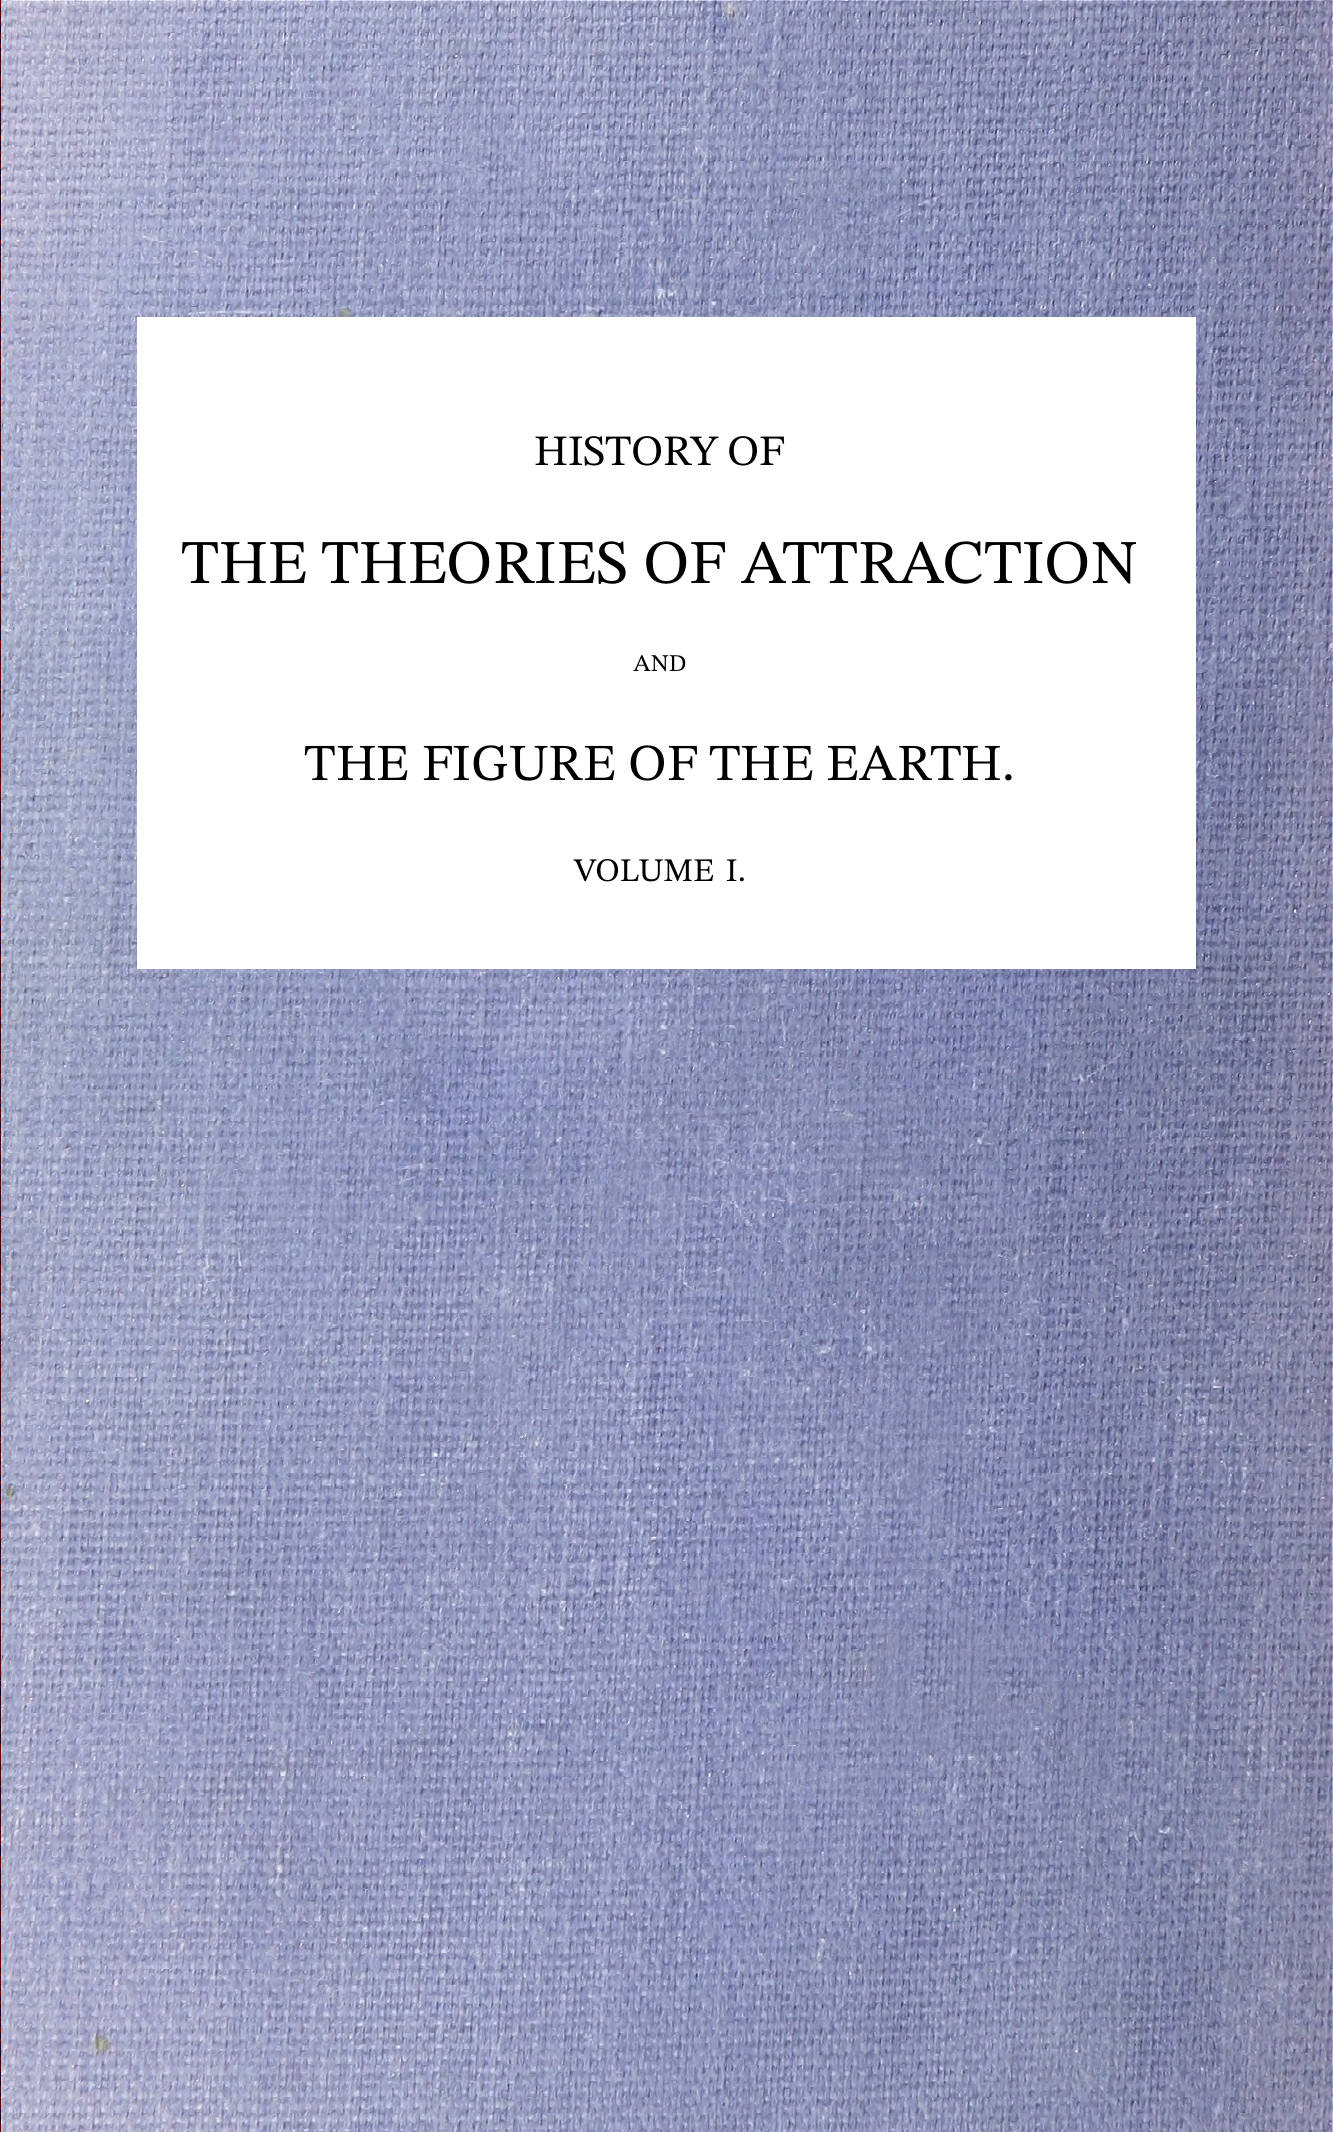
\includegraphics[width=0.999\textwidth,height=0.999\textheight,keepaspectratio]{cover.jpg}
\centering
\end{figure}
\restoregeometry

\newpage
\begin{PGtext}
\begin{center}
\large
\textbf{
The Project Gutenberg eBook of A history of the mathematical theories of attraction and the figure of the earth from the time of Newton to that of Laplace. Volume 1 by Isaac Todhunter
}
\end{center}
\InputIfFileExists{pgheader.tex}{}{}
\renewcommand*{\arraystretch}{1.5}
\begin{tabular}{p{2.5cm}>{\raggedright\arraybackslash}p{\dimexpr \linewidth-3.5cm}}
Title: &        A history of the mathematical theories of attraction and the figure of the earth from the time of Newton to that of Laplace. Volume 1\\
Author: &       Isaac Todhunter\\
Release Date: & January 21, 2023 [eBook \#69831]\\
Language: &     English\\
Credits: & The Online Distributed Proofreading Team at https://www.pgdp.net (This file was produced from images generously made available by The Internet Archive)\\
\end{tabular}
\vfill
\begin{center}
*** START OF THE PROJECT GUTENBERG EBOOK A history of the mathematical theories of attraction and the figure of the earth from the time of Newton to that of Laplace. Volume 1 ***
\end{center}
\end{PGtext}

\pagestyle{fancy}
\fancyhf{}
\fancyhead[R]{\thepage}

\frontmatter
\fontdimen2\font=0.75ex% inter word space
\textit{\fontdimen2\font=0.75ex}
{\small{\fontdimen2\font=0.75ex}}
%%-----File: 001.png-----%%
\thispagestyle{empty}
\hspace{0pt}
\vfill
\begin{center}
\large
HISTORY OF\\[0.5cm]
\LARGE
THE THEORIES OF ATTRACTION\\[0.7cm]
\scriptsize
AND\\[0.5cm]
\Large
THE FIGURE OF THE EARTH.\\[0.7cm]
\small
VOLUME I.
\vfill
\end{center}
%%-----File: 002.png-----%%
\newpage
\thispagestyle{empty}
\hspace{0pt}
\vfill
\small
Cet admirable Ouvrage [Newton's \textit{Principia}] contient les germes de
toutes les grandes découvertes qui ont été faites depuis sur le système du
monde: l'histoire de leur développement par les successeurs de ce grand
géomètre serait à la fois le plus utile commentaire de son Ouvrage, et
le meilleur guide pour arriver à de nouvelles découvertes.

\hspace*{\fill}
\textsc{Laplace.} \textit{Connaissance des Tems pour l'an} 1823.
\hspace{1cm}
\vfill
%%-----File: 003.png-----%%
\newpage
\thispagestyle{empty}
\begin{center}
\large
\textls[200]{A HISTORY}\\ [0.6cm]
\scriptsize
OF THE\\[0.5cm]
\LARGE
\scalebox{.8}[1.0]{MATHEMATICAL THEORIES OF ATTRACTION}\\ [0.7cm]
\scriptsize
AND\\ [0.5cm]
\Large
THE FIGURE OF THE EARTH,\\ [1cm]
\normalsize
\textit{FROM THE TIME OF NEWTON TO THAT\\
OF LAPLACE.}\\ [2cm]
\scriptsize
BY\\ [0.4cm]
\large
I. TODHUNTER, M.A., F.R.S.\\ [1.2cm]
\normalsize
\textit{IN TWO VOLUMES.}\\[0.4cm]
VOLUME I.\\ [1.3cm]
{\large\gfont{London:}}\\[0.2cm]
\textls[150]{MACMILLAN AND CO}.\\[0.2cm]
1873.\\[0.4cm]
{[}\textit{All Rights reserved.}{]}
\end{center}
%%-----File: 004.png-----%%
\newpage
\thispagestyle{empty}
\hspace{0pt}
\vfill
\begin{center}
{\large\gfont{Cambridge:}}\\[0.2cm]
\scriptsize
PRINTED BY C. J. CLAY, M.A.\\[0.2cm]
AT THE UNIVERSITY PRESS.
\end{center}
\vfill
%%-----File: 005.png-----%%
\Chapter{PREFACE.}
\Runhead{\textsc{preface.}}
\normalsize

\setlength\parskip{0pt plus1pt}
\textsc{In} the volumes now offered to students I have written the
history of an important branch of science in the manner in which
I formerly treated the Calculus of Variations and the mathematical
theory of Probability; and in the present work, as in
those, I undertake a task hitherto unattempted. For although
much has been published on the History of Astronomy, yet the
progress of the mathematical development of the principle of
Attraction has been left almost untouched. The last of the six
volumes which constitute the great work of Delambre is devoted
to the Astronomy of the eighteenth century; but the Astronomy
discussed is almost entirely that of observation, and the investigations
of the eminent mathematicians who contributed to fill up
the outline traced by Newton are scarcely noticed. There are
indeed interesting and valuable works in which the results
obtained by theory are stated in popular language for the benefit
of general readers; such is the well-known history by Bailly in
French, with its continuation by Voiron; and in English we
have various excellent productions of the same kind, especially
Narrien's \textit{Historical Account of the Origin and Progress of Astronomy},
and Grant's \textit{History of Physical Astronomy}. But the object
of these works is quite distinct from that which I have kept in
view in my contributions to scientific history. I desire not merely
to record the results which may have been obtained but to trace
the analysis which led to those results, to estimate its value, and
to discriminate between its failure and its success, its error and its
truth. So far as I know the only example of a mathematical
treatise bearing on the history of Physical Astronomy is Gautier's
\textit{Essai Historique sur le problême des trois corps}: but as this treats
of the Lunar and Planetary Theories, omitting the Figure of the
Bodies, it has nothing in common with the present work.

In the fifth volume of the \textit{Mécanique Céleste} Laplace arranges
the whole subject of Physical Astronomy in six divisions, and
gives brief sketches of the progress of the theory of all: in every
case sound knowledge practically begins with Newton. Laplace's
first division is devoted to the Figure and Rotation of the Earth;
and this has suggested to me the subject of the present work. I
%%-----File: 006.png-----%%
undertake accordingly to trace the history of the Theories of
Attraction and of the Figure of the Earth from Newton to Laplace.
The two subjects are necessarily associated in origin, and have
been historically always united; they are discussed together by
Laplace in the second volume of his great work. I have confined
myself to a single division of the wide subject of Physical Astronomy,
for the extent and difficulty of the whole might deter even
a professional cultivator of the science; and the numerous unfinished
fragments of works intended to bear on the \textit{Mécanique
Céleste} furnish an impressive warning against the rashness of any
extravagant design.

I will now give an outline of the plan of my work. The first
Chapter is necessarily occupied with Newton, the founder of Physical
Astronomy. The power revealed in all his efforts is nowhere
more conspicuous than in his treatment of our two subjects.

In the theory of attraction, among other important results, he
shewed that the attraction of a spherical shell on an external
particle is the same as if the shell were collected at its centre, and
that the attraction on an internal particle is zero. These two propositions
constitute a complete theory of the attraction of a sphere
in which the density varies as the distance from the centre. Moreover
the result with respect to an internal particle was extended
by Newton to the case in which the bounding surfaces of the shell
are similar, similarly situated, and concentric ellipsoids of revolution.

Newton originated the idea of investigating the Figure of the
Earth on the supposition that it might be treated as a homogeneous
fluid rotating with uniform angular velocity. He assumed as a
postulate that there could be relative equilibrium in such a case
if the form were that of an oblate ellipsoid of revolution; and he
determined the ratio of the axes and the law of variation of
gravity at the surface. The investigation, though not free from
imperfection, is a rare example of success in the first discussion of
a most difficult problem, and constitutes an enduring monument
to the surpassing ability of its author.

The second Chapter is devoted to Huygens. To him we owe
the important condition of fluid equilibrium, that the resultant
force at any point of the free surface must be normal to
the surface at that point; and this has indirectly promoted the
knowledge of our subject. But Huygens never accepted the great
principle of the mutual attraction of particles of matter; and thus
he contributed explicitly only the solution of a theoretical problem,
namely the investigation of the form of the surface of rotating
fluid under the action of a force always directed to a fixed point.
%%-----File: 007.png-----%%

The third Chapter treats of various miscellaneous investigations
connected with the subject in the course of one generation
after the publication of the \textit{Principia}. No real addition was
made to Newton's theoretical results, while the measurements
of arcs of the meridian in France led the Cassinis to adopt the
hypothesis that the form of the Earth was not oblate but oblong.

The fourth Chapter relates to Maupertuis. He wrote various
memoirs, among which were two in the form of commentaries on
Newton's theories of Attraction and the Figure of the Earth.
These theories were rendered more accessible by the translation
from their original geometrical expression into the familiar analytical
language of the epoch. By adhering to Newton's conclusions
Maupertuis must have contributed much to maintain the
truth among his countrymen, in opposition to the errors recommended
by the authority of Des Cartes and the Cassinis.

The important postulate assumed by Newton was first considered
by Stirling, a mathematician of great power: the fifth
Chapter shews that he obtained, at least implicitly, an approximate
demonstration of the required result.

In the sixth Chapter an account is given of various memoirs
by Clairaut which preceded the publication of his important work
on the Figure of the Earth. Clairaut explicitly demonstrated the
truth of Newton's postulate approximately. He also gave the
theorem, called Clairaut's theorem, which establishes a connection
between the ellipticity of the earth and the coefficient of the term
expressing the increase of gravity in passing from the equator to
the pole.

The seventh Chapter narrates briefly the circumstances of the
measurement of an arc of the meridian in Lapland. I have
undertaken to develop the progress of the Mathematical Theories
of Attraction and of the Figure of the Earth; but I do not profess
to include the practical operations conducive to our knowledge of
the exact dimensions of the Earth. These consist mainly of observations
of pendulums, and measurements of arcs; and an account
of them drawn from the original sources would form an interesting
and instructive work. But the more difficult matters to
which I have devoted the present volumes have furnished ample
employment without any serious divergence into the department
of practical application. I have therefore limited myself to short
notices of the earlier pendulum experiments, and of the two great
measurements in Lapland and Peru; these measurements deserve
some attention on account of their historical interest and their
decisive testimony to the oblate form of the Earth.

The eighth Chapter treats of various miscellaneous investigations
between 1721 and 1740. Desaguliers maintained, with
%%-----File: 008.png-----%%
a zeal not uniformly discreet, the oblate form against the Cassinian
hypothesis; on the other hand, the measurements in France were
still held to be in favour of that hypothesis. Towards the end
of the period the Academy of Paris proposed the Tides as the
subject of a Prize Essay; and this led to the important researches
of Maclaurin.

The ninth Chapter is devoted to Maclaurin. He completely
solved the problem of the attraction of an ellipsoid of revolution
on an internal or superficial particle; and his method
and results admitted of obvious extension to the case of an
ellipsoid not of revolution. The extent to which he proceeded
for the case of an external particle requires to be stated with
accuracy, in order to correct errors of opposite kinds which are
current. The most general result yet attained may be stated
thus: the potentials of two confocal ellipsoids at a given point external
to both are as their masses. This theorem was first established
by Laplace, but Maclaurin demonstrated it for the particular
case in which the external point is on the prolongation
of an axis of the ellipsoids. In the theory of the Figure of the
Earth, Maclaurin's main achievement was an exact demonstration
of Newton's postulate, of which hitherto only approximate
investigations had been given.

In the tenth Chapter the contributions of Thomas Simpson
are noticed. This eminent mathematician explicitly shewed that
if the angular velocity of rotation exceeds a certain value, the
oblatum is not a possible form of relative equilibrium for a fluid
mass; and it followed implicitly from his results that for any
value of the angular velocity less than the limit, more than one
figure for relative equilibrium would exist. Simpson also gave
a remarkable investigation of the attraction at the surface of a
very extensive class of nearly spherical bodies.

The eleventh Chapter consists of an analysis of the celebrated
work by Clairaut. The first part of the work treats on the
principles of fluid equilibrium; here Clairaut far surpassed his
predecessors in extent and accuracy, and left the theory in the
form which it still retains, with the single exception of the improvement
effected by Euler, who introduced the notion of the
pressure at any point of the fluid, together with the appropriate
symbol by which it is denoted. The second part of the work
treats on the Figure of the Earth. For the case of a homogeneous
fluid Clairaut closely followed Maclaurin. The case of a heterogeneous
fluid had been hitherto practically untouched, and Clairaut
invented for it a beautiful process which has remained substantially
unchanged to the present time; the chief result is a certain
equation connecting the ellipticity of the strata with their density,
%%-----File: 009.png-----%%
which appears in two forms: these I have called respectively
Clairaut's primary equation, and Clairaut's derived equation.

The twelfth Chapter narrates briefly the circumstances of the
measurement of an arc of the meridian in Peru. I have carefully
examined the extensive literature, much of which is controversial,
arising from this memorable expedition; and by means
of exact references I have afforded assistance to any student who
wishes to render himself familiar with all the circumstances.

The thirteenth Chapter is devoted to the earlier half of the
writings of D'Alembert which bear on our subjects. They are
extensive in amount, and may have served indirectly to diffuse
the interest in such investigations which the writer must have
felt himself; but on account of errors in principle and inaccuracy
of detail their direct value is small. In various attempts which
D'Alembert made to criticise the work of Clairaut he was I believe
almost uniformly wrong, so far as regards the Figure of the Earth,
and barely right on some unimportant points of Hydrostatics. It
is stated in the life of D'Alembert published in the \textit{Biographical
Dictionary of the Society for the Diffusion of Useful Knowledge}
that ``He and Clairaut were rivals, and no work of either appeared
without finding a severe critic in the other; but D'Alembert, the
more cautious and profound of the two, was generally on the right
side of the question:\dots'' The judgment is pronounced by a most
eminent authority to which I usually bow with reverence; but so
far as the subjects of the present work extend, I should venture to
reverse it.

The fourteenth Chapter is devoted principally to Boscovich,
whose writings furnish elementary accounts of the most important
results which had been obtained up to their date. I have also
given a brief notice of the poem by Stay, for which Boscovich
supplied notes and supplementary dissertations.

The fifteenth Chapter treats of various miscellaneous investigations
between the years 1741 and 1760. It includes a brief
notice of a Prize Essay on the Figure of the Earth, published by
Clairaut, some years after his treatise.

The sixteenth Chapter is occupied with the later half of the
writings of D'Alembert. The general character is the same as of
the earlier half; the investigations themselves are disfigured by
serious errors, but they serve to suggest interesting and important
matter.

The works of Frisi are noticed in the seventeenth Chapter:
they resemble those of Boscovich in the fact that they served to
teach the subject rather than to promote its progress.

The eighteenth Chapter treats of various miscellaneous investigations
between the years 1761 and 1780. The first three
%%-----File: 010.png-----%%
of Laplace's memoirs belong to this period, but for convenience the
consideration of them is postponed. The Chapter includes an account
of a memoir by Lagrange in which he proceeded by analysis
to the point Maclaurin had reached by geometry. The operations
carried on at Schehallien for ascertaining the density of the Earth
are noticed, and references are supplied to the subsequent labours
on the same subject. Here the first volume ends, which contains
the history of our subjects during the century which followed the
publication of Newton's \textit{Principia}.

The nineteenth Chapter takes the first three memoirs of
Laplace. The principal object of these memoirs may be said to
be the solution of a problem which is an extension of Newton's
postulate. Newton assumed that an oblatum was a possible form
of relative equilibrium for rotating fluid; the present problem is
to shew that an oblatum is the \textit{only} possible form, at least under
certain restrictions. I call the problem Legendre's, because he
was the first who solved it with tolerable success. D'Alembert
attempted the investigation, but failed. Laplace did not solve
the problem completely; but he shewed that for a very large
class of nearly spherical figures, the relative equilibrium was impossible.
He also obtained the expression for the law of gravity
which would hold universally.

The twentieth Chapter is devoted to a memoir which is conspicuous
in the history of the Theory of Attraction, namely the
earliest of Legendre's. The limit reached by Maclaurin is now for
the first time left behind; Legendre shews that the theorem with
respect to confocal ellipsoids is true for \textit{any position} of the external
point when the ellipsoids are solids of revolution. Legendre
introduces here the memorable expressions, hitherto unknown,
which are now usually called \textit{Laplace's coefficients}; and also, at the
suggestion of Laplace, the function now called the Potential function
takes its place in the subject.

The twenty-first Chapter brings before us a scarce treatise by
Laplace, and gives an analysis of that half of it which relates to
Attraction and the Figure of the Earth. Here was published for the
first time, the demonstration of the theorem relating to the action
of confocal ellipsoids at an external point which I call by Laplace's
name. The subjects of the Attraction of Ellipsoids and of the
homogeneous Figure of the Earth appear in this treatise in nearly
the same form as in the \textit{Mécanique Céleste}.

The twenty-second Chapter relates to Legendre's second memoir.
Here Legendre solves the problem which I call by his
name. He assumes that the fluid is in the form of a figure of
revolution, and that it does not deviate widely from the spherical
form.
%%-----File: 011.png-----%%

The twenty-third Chapter notices Laplace's fourth, fifth, and
sixth memoirs. The fourth and fifth memoirs contain the theory
of the attraction of spheroids, and the theory of Laplace's functions,
in the form they assume in the \textit{Mécanique Céleste}. The sixth
memoir relates to Saturn's ring.

The twenty-fourth Chapter is devoted to Legendre's third
memoir. The object of this memoir is to demonstrate Laplace's
theorem respecting confocal ellipsoids by a more direct process
than Laplace himself had employed. Legendre does demonstrate
the theorem, without expanding his expressions in series, but the
process is excessively long and complicated.

The twenty-fifth Chapter analyses Legendre's fourth memoir.
Here we have a great development of Clairaut's process for the
case of heterogeneous fluid. A general equation is obtained
analogous to Clairaut's primary equation; and from this it is
shewn that the strata must be ellipsoidal.

The twenty-sixth Chapter is devoted to Laplace's seventh memoir.
This contains some numerical discussion of the lengths of
degrees, and of the lengths of the seconds pendulum; there is also
a theory of the heterogeneous figure of the Earth, which substantially
agrees with that in Legendre's fourth memoir.

The twenty-seventh Chapter treats of miscellaneous investigations
between the years 1781 and 1800. Among other matters we
have here to notice Cousin's Introduction to the study of Physical
Astronomy, a memoir by Lagrange, and a memoir by Trembley;
the last is of the same unsatisfactory character as various memoirs
by the same writer which I have examined in my \textit{History of the
Mathematical Theory of Probability}.

The twenty-eighth Chapter gives an account of the first two
volumes of the \textit{Mécanique Céleste}, so far as they relate to our
subjects. Laplace in effect reproduced with small change the last
four of his seven memoirs; and the result is a treatise not yet
superseded.

The twenty-ninth Chapter traces the history of investigation
with respect to Laplace's Theorem. Ivory, Legendre, Gauss and
Rodrigues all gave complete discussions of the attraction of ellipsoids;
while Biot and Plana also commented on parts of the theory.
The method of Ivory is the simplest of all, and has obtained a
permanent position in our elementary works; insomuch that it is
usual to speak of \textit{Ivory's theorem}, although the more correct phrase
would be \textit{Ivory's demonstration of Laplace's theorem}.

The thirtieth Chapter treats on an equation which Laplace
seems to have regarded with peculiar favour, and which occurs
often in his writings. The equation however did not satisfy Ivory,
and he criticised it with severity. The result of the discussion
%%-----File: 012.png-----%%
may be said to have established the accuracy of Laplace's equation
when used, as he himself used it, with due caution. But at the
same time the objects which Laplace sought by the aid of his
equation are now generally obtained without it; so that practically
the equation is at present rarely employed.

The thirty-first Chapter elucidates the partial differential
equation for the symbol which denotes the potential function.
Laplace had originally assumed that a certain equation held both
for an external particle, and for a component particle of the body
considered; but Poisson shewed that the two cases required
different forms of the equation.

The thirty-second Chapter discusses a method which Laplace
gave for solving Legendre's problem, with the objection brought
against it by Liouville, and the treatment which Poisson substituted
in place of Laplace's.

The thirty-third Chapter passes in review various memoirs which
Laplace published during the first quarter of the present century.

The thirty-fourth Chapter is devoted to that part of the fifth
volume of the \textit{Mécanique Céleste} which relates to our subjects; it
consists chiefly of a republication of the memoirs noticed in the
thirty-third Chapter.

Strictly speaking the period of history which I proposed to
describe closes here; but it seemed convenient to include within
my range all the writings of three mathematicians who had
already been prominent in my work, and who may be naturally
associated with their predecessors, especially with Laplace. These
writers are Poisson, Ivory and Plana.

The thirty-fifth Chapter contains an account of all Poisson's
contributions which had not been previously examined. The most
important of these are an elaborate memoir on the Attraction of
Spheroids, and a memoir giving a new investigation of Laplace's
theorem respecting confocal ellipsoids.

The thirty-sixth Chapter gives a brief sketch of the numerous
articles and memoirs which Ivory produced, mainly in support of
opinions of his own which were both peculiar and erroneous. The
great promise which his early success held out was not followed by
any corresponding merit in the essays of his later years.

The thirty-seventh Chapter is devoted to Plana, who wrote
several papers chiefly in the form of comments on Lagrange,
Legendre and Laplace.

The last Chapter treats of various miscellaneous investigations
during the first quarter of the present century. It is by accident
the history finishes with a paragraph relating to Bowditch; but
on account of his moral and intellectual eminence, and of his
unselfish devotion to science, the name of one of the most distinguished
%%-----File: 013.png-----%%
mathematicians beyond the Atlantic may justly close a
roll which commences with that of Newton.

The period of time which I have traversed will be found to
correspond with some accuracy to a distinct boundary line in the
subject. The labours of more recent date present to us many indications
of what may be more appropriately called new methods
rather than mere developments of those already discussed. Among
them we may mention the investigations respecting the Potential
by Green and Gauss, and the numerous researches on the attraction
of Ellipsoids by Chasles; all these writers will occupy
conspicuous places in any future record of the subjects. Sir John
Herschel spoke of my \textit{History of Probability} as embracing the series
of the \textit{Pleiocene analysts} in distinction from the Post-Pleiocene;
and the illustration might be similarly applied in the present case.

Such then is the outline of the history which the present
volumes contain. The principles on which I have executed my
task are the same as those adopted in my former works; and
I may refer especially to the preface to my \textit{History of Probability}
for an account of them. I will only state here that I have not
thought it necessary to preserve the exact notation of the original
authors; that notation frequently varies much in various places,
and it is really advantageous for the sake of brevity and clearness
to use the same symbols throughout. For example the ratio of
the centrifugal force at the equator to the gravity there is denoted
in some English books by the letter \(m\); Clairaut uses \(\phi\);
D'Alembert in the sixth volume of his \textit{Opuscules Mathématiques}
uses \(\omega\); Laplace in the \textit{Mécanique Céleste}, Vol.\ \textsc{v}.\ page 7, uses \(\phi\),
and in Vol.\ \textsc{v}.\ page 23 he uses \(\alpha\phi\). For the ratio of the centrifugal
force at the equator to the attraction there, which is very
approximately the same thing as the preceding ratio, the letter \(j\)
is used throughout the present work.

I have been very sparing in the introduction of new terms,
for this practice seems carried to an embarrassing extent in some
modern mathematical works. I have however found it necessary
to have short designations for two things which occur perpetually
in these investigations. The body formed by the revolution of an
ellipse round its minor axis I call an \textit{oblatum}, and the body formed
by the revolution of an ellipse round its major axis I call an \textit{oblongum}.
In English books the former has usually been called an
\textit{oblate spheroid}; and the latter a \textit{prolate spheroid}. Something is
gained in conciseness by using one word instead of two for a name
which is frequently required; but the chief reason of the change
arises from the fact that the word \textit{spheroid} has been much used
in a different sense, namely to denote a body which differs but
little from a sphere. It would be very convenient if this sense
%%-----File: 014.png-----%%
of the word \textit{spheroid} could be so established as to render superfluous
the formal enunciation of the condition of resemblance to a sphere.
Perhaps the use of a word to express a form only approximately
determined is felt to be somewhat unlike the ordinary precision
of mathematical language; and this may account for the frequent
repetition of the condition even after it has been explicitly adopted.
Moreover the great French writers have often employed the word
\textit{spheroid} in a sense so wide as to render it practically equivalent
to \textit{body}; an example will be found in the title of a memoir by
Poisson on page 388 of the second volume.

I have found it convenient to give a name to a certain ratio
which is of importance in our subject, namely the ratio of the
difference of gravity at the equator and at the pole to gravity at
the equator. This ratio is one of the elements connected by
Clairaut's theorem, and I have accordingly called it \textit{Clairaut's
fraction}.

There is one term, perhaps the most objectionable of all that
have become permanent in mixed mathematics, which is used
throughout the work, namely \textit{centrifugal force}. It is with great
reluctance that I have felt myself constrained to yield to universal
authority and to employ language which experience shews
to be most perplexing and misleading. The well-trained student
will however have learned that the so-called centrifugal force is a
fiction; the simple fact is that a dynamical problem relating to
a body which is rotating uniformly, can be reduced to a statical
problem by supposing the rotation to cease and a certain force
to be introduced.

This History assumes on the part of the reader some elementary
acquaintance with the subjects on which it treats. For the Theory
of Attractions the Chapter in my work on \textit{Statics}, to which I
have occasionally referred, will be sufficient. For the Figure of
the Earth the student may consult three well-known English
treatises, namely one in Airy's \textit{Mathematical Tracts}, one in
O'Brien's \textit{Mathematical Tracts}, and Pratt's Chapter on the subject
in his \textit{Mechanical Philosophy}, afterwards enlarged and published
separately in a Treatise on \textit{Attractions, Laplace's Functions and
the Figure of the Earth}: Pratt's Treatise is the most comprehensive
of these English treatises, and the easiest to procure. An
interesting work was published at Paris in 1865, entitled \textit{Traité
Elémentaire de Mécanique Céleste. Par H. Resal}. About a third
of this volume is devoted to our subjects; and it gives a very
instructive account of them: but the extreme inaccuracy of the
printing is a serious diminution of the value of the work.

The mathematical expressions which are called \textit{Laplace's
coefficients} and \textit{Laplace's functions} play a very important part in
%%-----File: 015.png-----%%
the higher investigations of our subjects. The treatises of O'Brien,
Pratt, and Resal, which have just been cited contain a sufficient
account of these expressions for elementary purposes. The
student who wishes to become intimately acquainted with them
will have recourse to the work by Heine which is named on
page 24 of the second volume; this is an admirable volume
enriched with numerous references to the original authorities.

It may be naturally expected that a person who has devoted
much time to the study of the history of science will feel disposed
to attribute considerable value to the pursuit. The interest which
attaches to the struggle of the human mind with serious difficulties,
to its gradual progress and final triumph, may be at least as
great as that which is excited by an account of the vicissitudes of
civil history. An acquaintance with the origin and the course of
any science will often give great assistance in the comprehension of
its present state, and may even point out the most promising direction
for future efforts. Moreover a familiarity with what has been
already accomplished or attempted in any subject is conducive to
a wise economy of labour; for it may often prevent a writer from
investigating afresh what has been already settled, or it may
warn him by the failure of his predecessors, that he should not
too lightly undertake a labour of well-recognised difficulty. The
opinions of Laplace and Arago, which are quoted in my title-pages,
are justly entitled to great weight on these points.

That the subjects here treated historically are of no common
importance and influence may be easily seen. A knowledge of the
figure and dimensions of the Earth is the basis of all the numerical
results of Astronomy, and therefore of the greatest practical value.
Moreover the researches into the theories of Attraction and of the
Figure of the Earth have been fertile in yielding new resources
for mathematicians; it will be sufficient to point to the Transformation
of Multiple Integrals, the theory of the Potential, and the
elaborate doctrine of Laplace's functions, which have all sprung up
in the cultivation of this field of Physical Astronomy. Humboldt
has drawn attention to this circumstance in his \textit{Cosmos}; the following
passage occurs on pages 156 and 157 of the fifth edition
of Sabine's translation of the first Volume: ``Except the investigations
concerning the parallax of the fixed stars, which led to
the discovery of aberration and nutation, the history of science
presents no problem in which the object obtained,--the knowledge
of the mean compression of the Earth, and the certainty that its
figure is not a regular one,--is so far surpassed in importance by
the incidental gain which, in the course of its long and arduous
pursuit, has accrued in the general cultivation and advancement
of mathematical and astronomical knowledge.''
%%-----File: 016.png-----%%

It may appear that some apology is due for the extent to
which the work has grown; this must be found in the extent and
intricacy of the materials which had to be analysed. Indeed
Ivory, who devoted much attention to the subject of the Figure of
the Earth, asserts that it has been attended with greater difficulty
and has occasioned a greater number of memoirs than any other
branch of the system of the world. I have had some trouble in
keeping within the limits of two volumes, and have been compelled
to omit many developments which I should gladly have
printed. I have also published separately various papers which
have grown out of my historical studies; to these I refer in the
appropriate places, but it may be convenient to give a list of them
here. They are the following:

\Section
On Jacobi's Theorem respecting the relative equilibrium of a
revolving ellipsoid of fluid, and on Ivory's discussion of the
Theorem. \textit{Proceedings of the Royal Society}, Vol.\ \textsc{xix}.

Note relating to the Attraction of Spheroids. \textit{Proceedings of
the Royal Society}, Vol.\ \textsc{xx}.

Note on an erroneous extension of Jacobi's Theorem. \textit{Proceedings
of the Royal Society}, Vol.\ \textsc{xxi}.

On the Arc of the Meridian measured in Lapland. \textit{Transactions
of the Cambridge Philosophical Society}, Vol.\ \textsc{xii}.

On the equation which determines the form of the strata in
Legendre's and Laplace's theory of the Figure of the Earth.
\textit{Transactions of the Cambridge Philosophical Society}, Vol.\ \textsc{xii}.

On the Proposition 38 of the Third Book of Newton's \textit{Principia}.
\textit{Monthly Notices of the Royal Astronomical Society}, Vol.\ \textsc{xxxii}.

On the Arc of the Meridian measured in South Africa.
\textit{Monthly Notices of the Royal Astronomical Society}, Vol.\ \textsc{xxxiii}.

\Section
The account which is given of the memoirs and treatises
will be found ample enough in most cases to supply all that a
student will ever want to read of them; but this does not apply to
the \textit{Mécanique Céleste}, which I desire to illustrate not to supersede.
In other words all that I say relative to that great work is
intended as a commentary for the use of those who are consulting
the original. I have usually cited it by \textit{sections}, but in some
cases, which occur almost exclusively in the fifth volume, I have
for greater distinctness cited it by \textit{pages}. The pages meant are
those of Laplace's own edition; but the student who uses the
national edition will be able to adjust the references by observing
that in the fifth volume the 85 pages with which we are concerned
correspond to 103 pages in the national edition.

It is well known that Laplace does not give any specific
%%-----File: 017.png-----%%
references to the labours of his predecessors and contemporaries;
in his great treatises on Physical Astronomy and Probability he
embodied with his own results much that he derived from others,
and as these treatises have become the standards of authority for
the subjects to which they relate, it has followed that with uncritical
readers Laplace has not unfrequently obtained credit for
what was not distinctively his own production. A student of the
course of science will often discover that important investigations
which first came under his notice in the works of Laplace, are
really due to other mathematicians; and by a natural reaction
the conjecture will arise that further research will lead to the
restitution of much more to the rightful owners; and thus there
may be a recoil from an undue admiration to a suspicious depreciation.
But a complete evolution of the history will restore the
reputation of Laplace to its just eminence. The advance of
mathematical science is on the whole remarkably gradual, for
with the single exception of Newton there is very little exhibition
of great and sudden developments; but the possessions of one
generation are received, augmented, and transmitted by the next.
It may be confidently maintained that no single person has
contributed more to the general stock than Laplace.

In the life of Laplace in the \textit{English Cyclopædia}, which we
may safely attribute to the late Professor De Morgan, there are
some valuable remarks suggested by the want of specific information
in the writings of Laplace as to what was done by himself
and what was done by others; and it is stated that no one has
yet supplied the deficiency. With respect to Laplace it is said:
``Had he consulted his own glory, he would have taken care
always to note exactly that part of his own work in which he had
a forerunner; and it is not until this shall have been well and
precisely done, that his labours will receive their proper appreciation.''
In the present history and in that of Probability I have
gone over a third part of the collected mathematical works of
Laplace; and to that extent the evidence of his great power and
achievements is I hope fully and fairly manifested.

I have not hesitated to criticise all that has come before me;
and there is scarcely any memoir or treatise of importance left
without the suggestion of corrections or additions. I cannot
venture to hope that I have uniformly escaped without any
obscurity or error. My readers will I trust excuse such blemishes,
arising partly from the nature of the task and partly from the
circumstance that only such leisure could be found for it as
remained amidst continuous occupation in elementary teaching
and writing. The work has thus furnished ample employment
for seven years of labour, with the exception of a necessary digression
%%-----File: 018.png-----%%
in order to explain and illustrate some peculiarities in the
Calculus of Variations. It was perhaps rash for a mere volunteer
to undertake so extensive a task; but in spite of the imperfections
with which it may have been accomplished, I am willing to
hope that the result will be a permanent addition to the literature
of Physical Astronomy.

It is not from any desire to challenge comparisons with illustrious
men, but merely to justify my estimate of the labour
involved, that I venture to quote the following opinion expressed
by the late Professor James Forbes in his \textit{Review of the Progress
of Mathematical and Physical Science}, and to extend its application
from pure to mixed mathematics: ``Specimens of what a
history of pure mathematics would be, and must be, are to be
found in the able `Reports' of Dr Peacock and Mr Leslie Ellis,
in the Transactions of the British Association for 1833, and 1846.
A glance at these profound and very technical essays will shew
the impossibility of a popular mode of treatment, while the difficulty
and labour of producing such summaries may be argued
from their exceeding rarity in this or any other language.''

I have to record my great obligations to the Rev. J. Sephton,
Head Master of the Liverpool Institute, formerly Fellow of St
Johns College, for his most valuable assistance in conducting the
work through the Press. To the Syndics of the University Press
I am indebted for their liberality in defraying the expenses of the
printing.

\setlength\parskip{5pt plus1pt}
\hspace*{\fill}
I. TODHUNTER.
\hspace{1cm}

\vspace{1cm}
\footnotesize
\hangindent=1.5cm
\textsc{St John's College, Cambridge,}\\
\textit{July}, 1873.
\normalsize

%%-----File: 019.png-----%%
\Chapter{CONTENTS.}
\Runhead{\textsc{contents.}}
\Lsubhead{VOLUME I.}
\tocentry{Chapter I\@. Newton}{
Publication of the Principia, 1. Attractions, 2. Spherical shell on an internal
particle, 3. Spherical shell on an external particle, 4. Lemma, 6.
Zone of an indefinitely thin spherical shell, 7. Sphere on an external
particle, 8. Sphere on an internal particle, 10. Solid of revolution on
a particle at any point of the axis, 13. Infinite plane lamina, 15.
Jesuits' edition, 16. Density of the Earth, 17. Figure of the Earth, 18.
Polar and equatorial canals of fluid, 19. Approximate estimate of attractions,
20. Oblatum and oblongum, 21. Remarks on the approximate
estimate, 22. Equilibrium of the canals, 23. Attraction, gravity, weight, 25.
Newton's value of the ellipticity, 26. Jupiter's figure, 29. Influence of
the Sun's heat, 30. Measured lengths of degrees, 32. Weight resolved
along the radius, 33. Increment of gravity, 34. Pendulums, 36.
Newton's error, 37. Table of the lengths of a degree, 39. Pendulums, 40.
The Cassinian hypothesis untrue, 43. Summary of results, 44. Laplace's
opinion, 45. Halley's opinion, 46.}

\tocentry{Chapter II\@. Huygens}{
Publication of the Discourse, 47. Date of composition, 49. Vortex, 50.
Air pump, and weight in a mine, 51. Pendulum at Cayenne, 52.
Principle in Hydrostatics, 53. Value of the ellipticity, 54. Equation, 55.
Result extended, 56. Remarks on the Principia, 59. The Sun's distance
from the Earth, 61. Resisting medium, 62. Huygens's problem, 64.
Mistake as to priority, 65.}

\tocentry{Chapter III\@. Miscellaneous Investigations up to
the year 1720}{
Norwood, 68. Pendulums, 69. The Arabian measure, 70. Norwood, 71.
Halley, 72. Burnet, Whiston, and Keill, 73. Incidental mistakes, 75.
%%-----File: 020.png-----%%
Keill's error, 76. Keill and Halley, 77. Keill and Bentley, 78. Keill
and Whiston, 79. Pendulums, 80. D. Cassini adopts Keill's error, 81.
Snell, 82. De La Hire, 83. D. Gregory, 84. Keill, 85. Quotations from
Keill and Arago, 87. Numerical result, 89. Pendulums, 90. Freind, 91.
J. Cassini, 92. Hermann, 93. Hermann's problem, 95. Quotations
from Hermann and Boscovich, 97. J. Cassini, 99. French arc, 100.
Mairan, 109. Invents a law of attraction, 113. Summary of results, 115.}

\tocentry{Chapter IV\@. Maupertuis}{
Saturn's ring, 117. First problem, 118. Second problem, 119. Figure des
Astres, 122. A difficulty, 124; see 725. Variable stars and nebulæ, 127.
On the laws of attraction, 128. Incidental statements, 130. Figure de la
Terre, 131. Figures des Corps Célestes, 132. Hydrostatical principles
of Newton and Huygens, 133. Mistake, 137. View of an obscure
passage in Newton, 138. Figure de la Terre, 140, 141, 142. Examen
désintéressé, 143.}

\tocentry{Chapter V. Stirling}{
Newton's postulate, 151. Sir J. Lubbock, 152. Resultant action at the surface
of an oblatum, 153. Pendulum, 155. Remarks on the merits of
Clairaut and Stirling, 156. Theory compared with fact, 157. Estimates
of Stirling, 158.}

\tocentry{Chapter VI\@. Clairaut}{
Geodesic curve, 160. Proposition in solid Geometry, 161. Arcs of meridian, 162.
Newton's postulate, 163. Approximate attraction of an oblatum
at the pole, 165. Fluid with variable density, 167. Unsatisfactory
with respect to Hydrostatics, 170. Clairaut's Fraction, and Clairaut's
Theorem, 171. Huygens's problem, 173. Hydrostatical principles, 174.
Geodesic curve, 177.}

\tocentry{Chapter VII\@. Arc of the Meridian Measured in Lapland}{
Peruvian company, 178. Lapland company, 179. Maupertuis's book, 181.
Outhier's book, 182. Selection of places, 184. Difference of latitude, 185.
Measurement of the base, 186. Difference of latitude redetermined, 189.
Hardships, 192. Incidental matters, 194. Ellipticity, 196. Svanberg, 197.
Celsius, 198. Reference for further information, 199.}

\tocentry{Chapter VIII\@. Miscellaneous Investigations Between
the years 1721 and 1740}{
Desaguliers, 200. Criticises the conclusions of J. Cassini, 201. Admits Keill's
error, 202. Criticises Mairan's memoir, 203. Considers the French arc, 204.
%%-----File: 021.png-----%%
An experiment, 205. Incidental matters, 206. Poleni, 209. De la
Croyere, 210. J. Cassini, 211. Godin, 213. La Condamine, 214. J.
Cassini, 215. Pendulum, 217. Manfredi, 218. Bouguer on Hydrostatics,
219. J. Cassini, 220. Prize Essay by John Bernoulli, 221.
Modes of determining the form of the Earth, 222, 223. Cassini de
Thury, 224. Pendulums, 225. Cassini de Thury, 226. Bouguer, 227.
Delisle, 228. Euler, 229. D. Bernoulli's Hydrodynamica, 230. Cassini
de Thury, 231. The Tides, 232. D. Bernoulli's Essay, 233. Euler's
Essay, 234. Arc between Paris and Amiens, 235. French arc, 236.
Remark on the error in Picard's base, 238. Jesuits' edition of the
Principia, 239. Winsheim, 240.}

\tocentry{Chapter IX\@. Maclaurin}{
Treatise of Fluxions, 241. Attractions, 242. Ellipsoid of revolution, 244.
Newton's Postulate, 245. Extends Newton's Hydrostatical principle, 246.
Value of gravity, 247. Level surfaces, 248. Newton's Postulate, 249.
Attraction of a sphere, 251. Of an ellipsoid of revolution at the equator
and pole, 252. Reference to Newton, Cotes, and Stirling, 253. Attraction
of confocal ellipsoids, 254. Maclaurin's demonstration, 255. Confocal
shells, 256. External particle in the plane of the equator, 257.
Maclaurin's results, 259. His investigations under-estimated, 260. Attraction
of an oblatum, 261. Application to rotating fluid, 262. Variable
density, 264. Attraction of oblatum of varying density, 266. Application
of Newton's Hydrostatical principle, 267. Objections, 269. Polar
and equatorial columns, 270. Jupiter, 272. Essay on the Tides, 275.
Maclaurin's death, 276.}

\tocentry{Chapter X\@. Thomas Simpson}{
Mathematical Dissertations, 277. Reference to Maclaurin, 278. Attraction of
an oblatum, 279. Value of a definite integral, 280. Values of two definite
integrals, 281. Relation between excentricity and the angular velocity, 283.
Limit of angular velocity, 284. Two solutions, 285. Conservation of
Areas, 286. Oblatum not homogeneous, 289. Attraction of Spheroids, 290.
Length of a Degree, 292. Fluxions, 293. Simpson's eminence as a
mathematician, 294.}

\tocentry{Chapter XI\@. Clairaut}{
Figure de la Terre, 295. Fluid equilibrium, 296. Cartesians and Newtonians,
297. Principle of Canals and Principle of Level Surfaces, 298.
Points of interest in the Introduction, 299. Clairaut's first part, 300.
Comparison between Clairaut and others, 301. Principle of Canals, 302.
%%-----File: 022.png-----%%
General reasoning, 303. Cases where equilibrium is impossible, 304.
Principles of Newton and Huygens, 305. Rotating fluid, 306. Complete
differential, 307. Principle of Level Surfaces, 308. Examples of fluid
equilibrium, 309. Bouguer's problem, 310. Polar Coordinates, 312.
Space of three dimensions, 313. Capillary attraction, 314. Heterogeneous
fluid, 315. Law of attraction, 316. Clairaut's second part, 317.
Homogeneous Figure of the Earth, 318. Jupiter, 319. Attraction of a
circular lamina, 320. Attraction of an oblatum, 321. Ellipticity, 322.
Fluid about a solid nucleus, 323. Particular cases, 324. Criticisms on
Newton, 325. Oblongum may be a possible form, 326. Case in which
the thickness of fluid is small, 327. Objection by D'Alembert and
Cousin, 328. The ellipticity is in general less when the fluid is heterogeneous
than when it is homogeneous, 329. Variation of gravity, 330. Attraction
of a circular lamina, 331. Of an oval lamina, 332. Proposition as to
the attraction of an ellipsoid of revolution, 333. Particle on the prolongation
of the axis of revolution, 334. Analytical verification of a result
obtained by Clairaut, 335. Gravity at the surface of the Earth: Clairaut's
Theorem, 336. Inaccurate statements which have been made, 337.
Applications of Clairaut's theorem, 338. Strata of varying density, 339.
Attraction of a shell, 340. Primary Equation, 341. Derived Equation,
343. Another form of the derived equation, 344. Example of a
particular law of density, 345. Clairaut's derived equation, 346. Case
in which the mass consists of fluid of two densities, 347. Limits for the
ellipticity of a planet, 348. Comparison of theory with observation, 349.
Laplace's opinion, 350.}

\tocentry{Chapter XII\@. Arc of the Meridian measured in
Peru}{
The Peruvian expedition started before the Lapland, 351. Literature of the
subject, 352. Course of the operations, 353. Difficulties encountered, 354.
Base of verification, 355. The astronomical part, 356. Discordance of
the observations, 357. Final result, 358. The Spanish operations, 359.
Return to Paris, 360. Miscellaneous points, 361. The Spanish account,
362. Bouguer's Figure de la Terre, 363. Summary, 364.}

\tocentry{Chapter XIII\@. D'Alembert}{
Treatise on Fluids, 365. Historical sketch, 366. Comparison between theory
and actual measurement, 367. Second edition, 368. Matters of interest,
369. Treatise on the Winds, 370. Two sentences quoted, 371.
Companion to Huygens's problem, 372. Attraction of a homogeneous
oblatum at its surface, 373. Spherical nucleus, 374. Results which
D'Alembert considers strange, 375. Oblate nucleus, 376. Particular
case of a formula given by Clairaut, 377. Criticism on Clairaut, 378.
%%-----File: 023.png-----%%
Incorrect statement, 379. Attraction at the surface of an ellipsoid, 380.
Error, 381. Contradiction and error, 382. Ellipsoidal nucleus, 383.
Precession of the Equinoxes, 384. Important numerical relation, 385.
Combination of D'Alembert's result with Clairaut's, 386. Example in the
Integral Calculus, 387. Hypothesis as to the structure of the Earth, 390.
Inequality, 391. Treatise on the Resistance of Fluids, 392. His hydrostatical
principle, 394. Failure in attempt at generalization, 397. Surfaces
of equal density not necessarily level surfaces, 400. Failure in
attempt to generalize Clairaut's theory, 404. Researches on the System
of the World, 409. Criticism on Euler, 411. Difference between theory
and observation, 416. Results of integration, 423. General formula
for the attraction of a spheroid, 424. Spherical nucleus, 426. Oblate
nucleus, 429. Criticism on Clairaut, 431. Attraction of spherical
shell, 434. Results of integration, 436. Attraction of a spheroid of
revolution, 437. Three general equations, 444. General estimate of his
researches, 452.}

\tocentry{Chapter XIV\@. Boscovich and Stay}{
The work by Boscovich and Le Maire, 454. Boscovich's dissertations, 457.
Follows Maclaurin's solution, 461. Criticises Hermann, 466. Criticises
D. Bernoulli, 469. Pendulums, 472. Suggestion, 476. Measures of a
degree of the meridian, 481. Criticises Euler, 483. Abstract of the
treatise, 489. Stay's poem, 490. Dugald Stewart's opinion, 491.
Specimens of Stay's verses, 493. Supplementary dissertations, 494.
Newton's error, 499. D. Bernoulli's opinion of Newton, 501. Measures
of arcs, 508. Criticises Maupertuis, 510. Method for discordant observations,
511. French translation, 513.}

\tocentry{Chapter XV\@. Miscellaneous Investigations between
the years 1741 and 1760}{
Pendulums, 515. Murdoch, 516. Bremond's translation, 521. Addition by
Murdoch, 522. Mairan, 526. Cassini de Thury, 527. Clairaut and
Buffon, 528. E. Zanottus, 529. La Condamine, 530. Silvabelle, 531.
Frisi and Short, 532. Defence of Newton, 534. Clairaut's reply to
Frisi, 535. Bouguer, 538. La Caille's voyage, 539. La Caille's arc, 541.
Maclear's arc, 542. La Lande, 543. Euler, 545. La Caille's reply
to Euler, 546. Hollmannus, 547. Euler, 548. La Caille, 549. La
Condamine, 550. Picard's base, 551. Walmesley, 552. La Caille, 553.
D'Arcy, 554. Clairaut's Prize Essay, 555. Edition of the Principia,
by Madame du Chastellet, 558. Lagrange on D'Alembert's paradox, 561.}

\tocentry{Chapter XVI\@. D'Alembert}{
Articles in the Encyclopédie, 564. Reply to Boscovich, 567. Paradox, 569.
Corrects former errors, 571. Fluid equilibrium, 574. Attempts to solve
%%-----File: 024.png-----%%
Legendre's problem, 575. Failure, 576. Sixth volume of the Opuscules
Mathématiques, 579. Two solutions of the problem of rotating fluid, 580.
The case of a very small angular velocity, 584. Only two solutions, 586.
Replies to the translator of Boscovich, 590. Attraction of mountains, 592.
Discussion of a problem, 596. An oblongum not an admissible form, 601.
Two analytical matters, 611. Generalisation of a former problem, 613.
Correction of a recent error, 618. Attraction of an ellipsoid, 625. Extension
of former problem, 629. Error, 630. Criticises Clairaut, 634.
Considers Maclaurin's theorem, 636. Atmosphere, 637. Equation to the
surface, 639. Letters to Lagrange, 643. Demonstrates Maclaurin's
theorem, 645. Rejects an important formula, 651. Investigates a theorem
given by Laplace, 652. Fluid equilibrium, 654. Unsound demonstration,
657. Summary of his contributions, 658.}

\tocentry{Chapter XVII\@. Frisi}{
De Gravitate, 660. Measurements hitherto made, 661. Extends a result of
Newton's, 662. Criticism on Newton, 663. Newton's error, 664. Cosmographia,
668. Suggestion as to La Caille's arc, 671. Mistake
corrected, 673. Newton's error, 676. Stability of equilibrium, 678.
Fontana, 679. Opera, 680. Silvabelle's problem, 682.}

\tocentry{Chapter XVIII\@. Miscellaneous Investigations
between the years 1761 and 1780}{
Frisi, 686. Krafft, 687. Error, 689. Sum of a series, 694. Osterwald, 696.
Michell, 697. Canterzanus, 698. E. Zanottus, 699. J. A. Euler, 700.
Lambert, 701. Liesganig, 702. Mason and Dixon, Maskelyne, 703.
Liesganig, 704. Cavendish, 705. La Condamine, 706. Lagrange, 707.
Transformation of variables, 710. Ellipsoid, 712. Beccaria, 717.
Cassini de Thury, 718. Lagrange, 720. Demonstrates Maclaurin's
theorem, 721. Cassini de Thury, 723. Schehallien experiment, 724.
Statement by Newton, 725. Dionis du Séjour, 728. Whitehurst, 729.
Hutton's calculations for Schehallien, 730. Playfair's survey of the
mountain, 731. Hutton, 732. Density of the Earth, 733. Cousin, 734.
Euler, 735. Hutton, 736. Titles of works, 738. Additional remarks, 740.}
%%-----File: 025.png-----%%

\newpage
\Lsubhead{VOLUME II.}
\tocentry{Chapter XIX\@. Laplace's First Three Memoirs}{
Five divisions in Laplace's writings, 741. First Memoir, 742. Legendre's
problem, 744. Second memoir, 751. Law of variation of gravity, 753.
Laplace's equation, 755. Third memoir, 764. Mistake, 769. Laplace's
equation, 771. Order of the writings of Laplace and Legendre, 778.}

\tocentry{Chapter XX\@. Legendre's First Memoir}{
Treatment of Maclaurin's theorem, 781. Extension of it, 782. Laplace's coefficients, 783.
Heine's work, 784. General expression for a coefficient, 786.
Potential, 789. Green and Gauss, 790. Legendre's theorem, 791. Criticism
on the demonstration, 792. Extension of Maclaurin's theorem, 793.
Character of the memoir, 794.}

\tocentry{Chapter XXI\@. Laplace's Treatise}{
Its scarcity, 796. Publication, 797. Number of sections, 800. Equation to
an ellipsoid, 801. Potential, 802. Polar coordinates, 803. Laplace's
theorem, 804. Attraction of an ellipsoid, 805. History of the problem, 806.
Rotating fluid mass, 807. Treatment of D'Alembert's problem, 808.
Case of the Moon, 809. Case of the Earth, 810. Two and only two
solutions, 811. Conservation of areas, 813. Laplace's equation, 814.
General problem of the form of fluid, 815. Law of gravity at the surface
of a fluid mass, 816. Spherical shell attracting external particle, 817.}

\tocentry{Chapter XXII\@. Legendre's Second Memoir}{
Object of the memoir to solve Legendre's problem, 820. Conditions of the
demonstration, 821. Seven theorems as to Laplace's coefficients, 822.
Equation to be solved, 831. Mode of treatment, 837. Remarks on the
demonstration, 842. Legendre's own opinion respecting it, 844. Quotation
from Laplace, 845. Quotation from Ivory, 846. Quotation from
Jacobi, 847.}

\tocentry{Chapter XXIII\@. Laplace's Fourth, Fifth, and
Sixth Memoirs}{
Fourth memoir, 848. Laplace's theorem, 850. Partial Differential Equation
for the Potential, 851. Laplace's Equation, 852. Error, 854. Property of
Laplace's functions, 857. Fifth memoir, 859. Degrees and Pendulums, 860.
Numerical example, 862. Oversight, 863. Sixth memoir, 864. Saturn's
ring, 865. Partial Differential Equation for the Potential, 866. Division
of Saturn's ring, 867. Form of the ring, 868. Plana's criticisms on
Laplace, 871. Instability of a ring, 872.}
%%-----File: 026.png-----%%

\tocentry{Chapter XXIV\@. Legendre's Third Memoir}{
Object of the memoir to demonstrate Laplace's Theorem, 875. Transformation
of multiple integrals, 877. Case in which the attracted particle is in a
principal plane of the ellipsoid, 880. General problem, 881. Point of the
Integral Calculus, 882. Legendre's theorem, 883. Limitation in Legendre's
process, 886. Opinions of the method, 887.}

\tocentry{Chapter XXV\@. Legendre's Fourth Memoir}{
Object of the memoir, 892. Error, 896. Laplace's coefficients, 897. First
hypothesis, 902. Result of first approximation, 909. Second approximation,
912. Ellipticity, 917. Length of degree, 918. General theorem, 920.
Force of gravity, 921. Clairaut's theorem, 923. Second hypothesis, 925.
Clairaut's equation generalised, 929. Vanishing of terms, 933. Examples
of laws of density, 939. First example; density constant, 940.
Second example, 941. Third example, 942. Second approximation, 943.
Third hypothesis, 944. Numerical values, 945. Case in which the figure
is not assumed to be one of revolution, 948. Laplace's functions, 949.
Correction of an oversight in Laplace, 953. The form of a planet must
be an oblatum, 955. General estimate, 957.}

\tocentry{Chapter XXVI\@. Laplace's Seventh Memoir}{
Mode of treating measured lengths of degrees, 960. Another method due to
Boscovich, 962. Lengths of seconds pendulum, 964. Two methods of
treatment, 966. Clairaut's Theorem, 967.}

\tocentry{Chapter XXVII\@. Miscellaneous Investigations
between the years 1781 AND 1800}{
Euler, 970. Krafft, 971. Error of B. St Pierre, 972. Cousin's Elementary
Treatise, 973. Error, 976. Approximate formulæ, 978. Attempts to
generalise Clairaut's theory, 980. Error, 982. Roy, 984. La Lande, 985.
Roy, 986. Embarrassed by an error of Bouguer's, 987. Williams, 988.
La Lande on Fernel's measure, 989. Legendre's Theorem in Spherical
Trigonometry, 990. Monge, 991. Borda and others, 992. Coulomb's
theorem, 993. Lagrange's Mécanique Analytique, 994. Waring, 995.
Triesnecker, 996. Pictet, 997. Waring, 998. Dalby, 999. Cassini IV.
and others, 1000. Cagnoli and Baily, 1001. Topping, 1002. La Lande's
Astronomie, 1003. Lagrange, 1004. Partially investigates Laplace's
theorem, 1008. Rumovsky, 1012. Prony, 1014. Cavendish, 1015.
Result as to the mean density of the Earth, 1018. Trembley, 1019.
Algebraical identity, 1024. Error, 1027. Legendre's coefficients, 1028.
Laplace's equation, 1030. Fontana, 1034. Van-Swinden, 1035. Survey
of England and Wales, 1036. General Roy's rule, 1037.}
%%-----File: 027.png-----%%

\tocentry{Chapter XXVIII\@. Laplace, Mécanique Céleste,
First and Second Volumes}{
First volume, 1041. Potential, 1042. Case of a spherical shell, 1043.
Objection, 1044. Spherical shell and external particle, 1045. Laplace's
enunciation extended, 1046. Spherical shell and internal particle, 1047.
Cylinder, 1048. Cylindrical shell, 1050. Second volume, 1052. First
Chapter, Spheroid, 1053. Attraction of an ellipsoid, 1054. Laplace's
theorem, 1060. Professor Cayley's paper, 1061. Second Chapter, Laplace's
functions, 1064. Various names for them, 1066. Any function may be
expanded in a series of them, 1067. Form of the expansion, 1069.
Legendre's theorem extended, 1076. Third Chapter, Oblatum, 1078.
His results, 1079. Sources of them, 1080. Oblongum inadmissible, 1082.
One oblatum for given moment of rotation, 1085. Fourth Chapter, 1088.
Bouguer's hypothesis rejected, 1094. Approximation extended, 1098.
Fifth Chapter, 1100. Misprints, 1102. Fifth Chapter, 1103. First
method of calculation, 1104. Second method, 1105. Jupiter, 1109.
Lapland arc, 1111. Arc perpendicular to the meridian, 1112. Sixth
Chapter, Saturn's ring, 1116. Attraction of an elliptic cylinder, 1119.
The resultant constant at the surface, 1123. Seventh Chapter, Atmosphere,
1126. Summary of results, 1127.}

\tocentry{Chapter XXIX\@. Laplace's Theorem}{
History of the Theorem, 1129. Biot's investigation, 1130. General theorem, 1133.
Particular case, 1136. Biot's historical statement questioned, 1138.
Ivory, 1140. His enunciation, 1143. Opinions of his merit, 1146.
Plana, 1147. Biot's appendix, 1148. Legendre, 1149. History of the
theorem, 1150. Expressions for the attraction of an ellipsoid, 1152.
Approximation for a nearly spherical body, 1155. Elliptic integrals, 1156.
Algebraical relation, 1157. Another relation, 1158. Poisson extends
Ivory's theorem, 1160. This does not apply to Laplace's theorem, 1161.
Gauss, 1162. His fifth theorem, 1169. His fourth theorem, 1170. His
third theorem, 1171. His sixth theorem, 1172. Application to the ellipsoid,
1173. Gauss's reference to Ivory, 1175. Rodrigues, 1176. Relative
Potential, 1179. Symmetrical expression for the Potential of an
ellipsoid, 1184. Formula for Legendre's coefficient, 1187. General property
of the coefficients, 1189. Summary of results, 1194.}

\tocentry{Chapter XXX\@. Laplace's Equation}{
Particular form, 1196. Lagrange, 1197. The difficulty which he explains, 1200.
Ivory's objections, 1203. History of the equation, 1204. The point of difficulty,
1207. Expansion in a series of Laplace's functions, 1213. General
form of the equation, 1214. Ivory's objections, 1215. Ivory's notice of
Lagrange's memoir, 1216. Second memoir by Ivory, 1219. Laplace's
later investigation, 1220. Poisson, 1223. Ivory returns to the subject,
%%-----File: 028.png-----%%
1224. Laplace's opinion of Ivory, 1226. Airy, 1227. His treatment
of the equation, 1228. Expansion in a series of Laplace's functions,
1230. Mc Cullagh, 1233. Plana, 1235.}

\tocentry{Chapter XXXI\@. Partial Differential Equation
for \(V\)}{
Laplace's equation, 1236. Poisson's correction, 1237. Applications, 1239.
Rodrigues, 1240. Poisson's later method, 1241. The three cases, 1244.
Objection, 1245. Ostrogradsky, 1247. Extends the unsatisfactory case
given by Poisson, 1248. Sturm, 1251. Bowditch, 1252. Gauss's criticism,
1253.}

\tocentry{Chapter XXXII\@. Laplace's Second Method of
treating Legendre's Problem}{
History of the problem, 1254. Liouville, 1255. Laplace's process, 1256. Limits
of the integration, 1261. Liouville's objection to Laplace's process, 1263.
Poisson's process, 1265. Remarks on it, 1267. Laplace's supplementary
investigation, 1270. Wantzel, 1272. Transformation of a double
integral, 1273.}

\tocentry{Chapter XXXIII\@. Laplace's Memoirs}{
Saturn's ring, 1275. Rotation of the Earth, 1276. Figure of the Earth, 1277.
Rotation of the Earth, 1278. Theorem as to a principal axis, 1281. Law
of gravity, 1283. Figure of the Earth, 1284. Cooling of the Earth, 1287.
Increase of temperature with increase of depth, 1290. Mean density of
the Earth, 1291. Extracts on Hutton, Cavendish and Newton; 1292.}

\tocentry{Chapter XXXIV\@. Fifth Volume of the Mécanique
Céleste}{
Eleventh Book, 1294. First Chapter, Historical sketch, 1295. Elephant
preserved in the ice, 1296. Second Chapter, Results obtained by Analysis,
1301. Value of gravity, 1305. Expression for the depth of the
sea, 1310. Value of gravity, 1313. Approximate values of Legendre's
functions, 1314. Variations of the lengths of degrees and of the value
of gravity, 1316. Expression for gravity at the surface of a supposed atmosphere,
1318. Comparison of the analysis with observations, 1320. Lunar
Theory, 1322. Measures of degrees, 1323. Precession and Nutation, 1324.
Hypothetical law connecting the pressure and the density, 1325.
Legendre's law of density, 1326. Numerical results, 1328. Young and
D. Bernoulli, 1330. Attraction of a mountain, 1332. Third Chapter, 1336.
Theorem as to the three principal axes, 1338. Transformation of angular
coordinates, 1340. Fourth Chapter, 1343. Fourier and Poisson, 1346.
Analytical results, 1350. Correction, 1351. General summary, 1354.}
%%-----File: 029.png-----%%

\tocentry{Chapter XXXV\@. Poisson}{
List of his writings, 1356. Memoir on electricity, 1357. Attraction of spheroids,
1358. Laplace's functions, 1360. Value of the potential, 1363.
Accurate distinction of cases, 1364. Partial differential equation for the
potential, 1365. Spheroids which differ little from spheres, 1367. A
point hitherto neglected now examined, 1368. Investigation carried to a
certain order, 1369. May be extended, 1371. Two forms coincide at the
surface, 1372. A transformation, 1373. Laplace's equation extended, 1374.
Application to rotating fluid, 1375. Novelties in the process, 1376. Approximation
to the second order, 1378. Coulomb's theorem, 1380. Heterogeneous
fluid, 1381. Partial differential equation for the potential, 1382.
Ivory's criticism, 1384. Addition to the memoir, 1385. Double integral,
1386. Argument against Ivory, 1388. Convergence of series, 1389.
Poisson's Mechanics, 1390. Attraction of ellipsoids, 1391. Remarkable
result, 1394. New forms for the component attractions, 1395.
Elliptic integrals, 1398. Note on a result given by Jacobi, 1401. Controversy
between Poisson and Poinsot, 1404. Poisson's remarks on
Poinsot's report, 1405. Poinsot's reply, 1408. Poisson's Addition, 1410.
Poinsot's reply, 1411. Remarks on the controversy, 1412. Note on the
general formulæ of attractions, 1413. Liouville's process of investigation,
1414. General summary, 1415.}

\tocentry{Chapter XXXVI\@. Ivory}{
List of his writings, 1416. Attraction of an extensive class of spheroids, 1417.
Expansion in a series, 1420. Equilibrium of a fluid, 1421. New principle assumed,
1422. Theorem on the Potential, 1424. Inconclusive reasoning, 1425.
True proposition, 1426. Proposition which is not necessarily true, 1427.
Error, 1428. Converse of a known result, 1429. Supposed solution of
Legendre's problem, 1430. Good treatment of a standard equation, 1432.
Unsupported assertion, 1433. Unintelligible reason, 1434. Article on
Attraction, 1435. Figure of the Earth, 1436. Fluid attracted to a fixt
centre, 1441. Proposed second approximation, 1442. Opinion on the
Theory of the Figure of the Earth, 1444. Criticisms on Professor Airy
and Poisson, 1445. Pronounces a certain theorem inaccurate, 1448.
Demonstrates the theorem, 1449. Criticises a remark made by Biot, 1453.
Erroneous statements, 1456. Ivory's assumed principle, 1459. Discusses
erroneously Jacobi's theorem, 1460. Remarks on Poisson, 1461. General
summary, 1464.}

\tocentry{Chapter XXXVII\@. Plana}{
List of his writings, 1465. Commentary on Lagrange, 1466. Problems in
Attraction, 1468. Erroneous result, 1472. Solution of a problem, 1474.
Neglect of the principle of dimensions, 1476. Saturn's ring, 1479.
Solution of a problem, 1480. Two definite integrals, 1484. Law of
%%-----File: 030.png-----%%
density and pressure, 1486. Formula given by Gauss, 1489. Law of
density, 1491. Attraction of ellipsoid, 1492. Opinion of Legendre's process,
1495. Criticises Legendre and Pontécoulant, 1498. Remark on Rodrigues,
1502. Unsupported statement, 1503. Remark on Legendre, 1505.
Refers to the example of Euler, 1507. Poisson and Legendre, 1508.
The potential of an ellipsoid, 1509. Appendix to the memoir on the
attraction of an ellipsoid, 1513. Notes on Newton, 1515. Opinion on
Newton's method, 1519. Density of the superficial stratum, 1520. Difficulties,
1524. Density of a mountain, 1527. Force of gravity, 1528.
Hypothesis of Huygens, 1529. Criticises Laplace, 1530. Attributes an
error to Newton, 1534. Criticises Calandrini, 1535. Approximate solution,
1538. Oblongum is not an admissible figure, 1539. Jacobi's
Theorem, 1540. Potential of an ellipsoid, 1543. Criticises Poisson, 1544.
Hypothesis of uniformly increasing density, 1546. Formula of the Integral
Calculus, 1550. Gravity at the surface of the sea, 1551. Laplace's
equation, 1553. Remark on D'Alembert, 1556. Tides, 1558. Remark
on Newton, 1559. General summary, 1560.}

\tocentry{Chapter XXXVIII Miscellaneous Investigations
Between the Years 1801 and 1825}{
Clay, 1562. Benzenberg, 1563. Burckhardt's translation of Laplace, 1564.
Other works of the same nature, 1565. Playfair, 1566. Length of arc of the
meridian, 1568. The Survey of England, 1572. Svanberg, 1575. Von
Zach, 1576. Base du Système Métrique, 1577. Dr Young, 1578. De
Zach, 1579. Lagrange, 1580. Example of Fluid equilibrium, 1581.
Error, 1582. Playfair, 1583. Silvabelle's problem, 1584. Error, 1587.
General result, 1589. Knight, 1593. Attraction of a right-angled
triangle, 1595. Extension of Silvabelle's problem, 1599. Modification of
the problem, 1601. Formula of the Integral Calculus, 1603. Solution of
an example, 1604. De Zach on the Attraction of mountains, 1605.
Quotations, 1607. Tadino, 1608. Cauchy, 1609. Dissertation on pendulums,
1610. Luckcock, 1611. Adrain, 1612. Lambton's Indian arc, 1614.
Nobili, 1615. Dr Young, 1616. The mean density of the Earth, 1617.
Dr Young's Rule, 1618. Ellipticity calculated, 1619. Erroneous solution
of a problem, 1621. General remarks, 1623. Wronski, 1624. Airy, 1625.
Saturn's ring, 1627. Different numerical calculations, 1628. Form of
Saturn, 1630. Beccaria's arc, 1631. Bowditch, 1632.}
%%-----File: 031.png-----%%

\newcommand{\andots}{\;\dotfill&\!\dotfill\;}
\Chapter{CHRONOLOGICAL LIST OF AUTHORS.}
\Subhead{\textit{The figures refer to the Articles of the Volumes.}}
\Runhead{\textsc{chronological list of authors.}}
\footnotesize
\begin{longtable}{l l @{} r}
& & \scriptsize{ART.}\\
\endhead
1637 & \textsc{Norwood}\andots 68, 71\\
1669 & \textsc{Picard}\andots 70, 102\\
&\textsc{Richer}\andots 69\\
&\textsc{Varin}\andots 69\\
&\textsc{Des Hayes}\andots 69\\
&\textsc{Du Glos}\andots 69\\
1686 & \textsc{Halley}\andots 72\\
1687 &\textsc{Newton}\andots 1\\
1690 &\textsc{Huygens}\andots 47\\
1691 &\textsc{Eisenschmidt}\andots 76\\
1698 &\textsc{Keill}\andots 73\\
1699 &\textsc{Keill}\andots 79\\
1700 &\textsc{Couplet}\andots 80\\
1701 &\textsc{Des Hayes}\andots 81\\
1701 &\textsc{D. Cassini}\andots 81\\
1702 &\textsc{J. Cassini}\andots 82\\
1702 &\textsc{D. Gregory}\andots 84\\
1703 &\textsc{De la Hire}\andots 83\\
1708 &\textsc{Krill}\andots 85\\
1708 &\textsc{Feuillée}\andots 90\\
1711 &\textsc{Freind}\andots 91\\
1713 &\textsc{Newton}\andots 1\\
1713 &\textsc{J. Cassini}\andots 92\\
1716 &\textsc{Hermann}\andots 93\\
1718 &\textsc{J. Cassini}\andots 99\\
1720 &\textsc{J. Cassini}\andots 100\\
1720 &\textsc{Mairan}\andots 109\\
1725 &\textsc{Desaguliers}\andots 200\\
1726 &\textsc{Newton}\andots 1\\
1728 &\textsc{Poleni}\andots 209\\
1729 &\textsc{De la Croyere}\andots 210\\
1732 &\textsc{Maupertuis}\andots 117, 122, 128\\
1732 &\textsc{J. Cassini}\andots 211\\
1733 &\textsc{Maupertuis}\andots 131\\
1733 &\textsc{Godin}\andots 213\\
1733 &\textsc{La Condamine}\andots 214\\
1733 &\textsc{J. Cassini}\andots 215\\
1733 &\textsc{Clairaut}\andots 160\\
1734 &\textsc{Maupertuis}\andots 132\\
1734 &\textsc{Bradley}\andots 217\\
1734 &\textsc{Manfredi}\andots 218\\
1734 &\textsc{Bouguer}\andots 219\\
1734 &\textsc{J. Cassini}\andots 220\\
1734 &\textsc{John Bernoulli}\andots 221\\
1735 &\textsc{Maupertuis}\andots 140\\
1735 &\textsc{Stirling}\andots 151\\
1735 &\textsc{Clairaut}\andots 161\\
1735 &\textsc{J. Cassini}\andots 222, 223\\
1735 &\textsc{Cassini de Thury}\andots 224\\
1735 &\textsc{Mairan}\andots 225\\
1735 &\textsc{Godin}\andots 225\\
1735 &\textsc{Bouguer}\andots 225\\
1735 &\textsc{La Condamine}\andots 225\\
1736 &\textsc{Maupertuis}\andots 141\\
1736 &\textsc{Clairaut}\andots 162\\
1736 &\textsc{Cassini de Thury}\andots 226\\
1736 &\textsc{Bouguer}\andots 227\\
1737 &\textsc{Maupertuis}\andots 142\\
1737 &\textsc{Clairaut}\andots 163\\
1737 &\textsc{Delisle}\andots 228\\
1738 &\textsc{Maupertuis}\andots 146, 150, 181\\
1738 &\textsc{Clairaut}\andots 167\\
1738 &\textsc{Celsius}\andots 181, 198\\
1738 &\textsc{Euler}\andots 229\\
1738 &\textsc{D. Bernoulli}\andots 230\\
1739 &\textsc{Clairaut}\andots 177\\
%%-----File: 032.png-----%%
1739 &\textsc{Cassini de Thury}\andots 231\\
1740 &\textsc{D. Bernoulli}\andots 233\\
1740 &\textsc{Euler}\andots 234\\
1740 &\textsc{Maupertuis}\andots 235\\
1740 &\textsc{Cassini de Thury}\andots 236\\
1740 &\textsc{Winsheim}\andots 240\\
1740 &\textsc{Maclaurin}\andots 275\\
1741 &\textsc{Murdoch}\andots 515\\
1742 &\textsc{Zeller}\andots 181\\
1742 &\textsc{Le Seur}\andots 239\\
1742 &\textsc{Jacquier}\andots 239\\
1742 &\textsc{Calandrinus}\andots 239\\
1742 &\textsc{Maclaurin}\andots 241\\
1742 &\textsc{Bremond}\andots 521\\
1742 &\textsc{Mairan}\andots 526\\
1743 &\textsc{Simpson}\andots 277\\
1743 &\textsc{Clairaut}\andots 295\\
1744 &\textsc{Outhier}\andots 182\\
1744 &\textsc{Bouguer}\andots 352\\
1744 &\textsc{D'Alembert}\andots 365\\
1744 &\textsc{Cassini de Thury}\andots 527\\
1745 &\textsc{La Condamine}\andots 352\\
1745 &\textsc{Buffon}\andots 528\\
1745 &\textsc{Clairaut}\andots 528\\
1746 &\textsc{Bouguer}\andots 352\\
1746 &\textsc{La Condamine}\andots 352\\
1746 &\textsc{Zanottus, E.}\andots 529\\
1747 &\textsc{D'Alembert}\andots 370\\
1747 &\textsc{La Condamine}\andots 530\\
1748 &\textsc{Juan}\andots 352\\
1748 &\textsc{Ulloa}\andots 352\\
1748 &\textsc{Cassini de Thury}\andots 530\\
1749 &\textsc{Bouguer}\andots 352\\
1749 &\textsc{D'Alembert}\andots 384\\
1749 &\textsc{Euler }\andots 411\\
1750 &\textsc{Simpson}\andots 293\\
1750 &\textsc{Silvabelle}\andots 531\\
1751 &\textsc{La Condamine}\andots 352\\
1751 &\textsc{Bouguer}\andots 538\\
1751 &\textsc{La Caille}\andots 539\\
1752 &\textsc{Bouguer}\andots 352\\
1752 &\textsc{La Condamine}\andots 352\\
1752 &\textsc{D'Alembert}\andots 392\\
1752 &\textsc{La Caille}\andots 539\\
1752 &\textsc{La Lande}\andots 543\\
1753 &\textsc{Frisi}\andots 532\\
1753 &\textsc{Short}\andots 532\\
1753 &\textsc{Clairaut}\andots 535\\
1753 &\textsc{La Lande}\andots 544\\
1753 &\textsc{Euler}\andots 545\\
1754 &\textsc{Bouguer}\andots 352\\
1754 &\textsc{La Condamine}\andots 352\\
1754 &\textsc{D'Alembert}\andots 410\\
1754 &\textsc{La Caille}\andots 546\\
1754 &\textsc{Hollmannus}\andots 547\\
1754 &\textsc{Bouguer} and others\andots 551\\
1755 &\textsc{Boscovich}\andots 454\\
1755 &\textsc{Euler}\andots 548\\
1755 &\textsc{La Caille}\andots 549\\
1756 &\textsc{D'Alembert}\andots 415, 564\\
1756 &\textsc{La Condamine}\andots 550\\
1757 &\textsc{Boscovich}\andots 489\\
1757 &\textsc{D'Alembert}\andots 565\\
1758 &\textsc{Walmesley}\andots 552\\
1758 &\textsc{La Caille}\andots 553\\
1758 &\textsc{D'Arcy}\andots 554\\
1759 &\textsc{Clairaut}\andots 555\\
1759 &\textsc{Chastellet}\andots 558\\
1759 &\textsc{Lagrange}\andots 561\\
1760 &\textsc{Boscovich}\andots 490\\
1760 &\textsc{Stay}\andots 490\\
1760 &\textsc{Lagrange}\andots 562\\
1761 &\textsc{D'Alembert}\andots 566\\
1761 &\textsc{Frisi}\andots 686\\
1763 &\textsc{La Caille}\andots 540\\
1764 &\textsc{Krafft}\andots 687\\
1764 &\textsc{Osterwald }\andots 696\\
1766 &\textsc{Michell}\andots 697\\
1767 &\textsc{Canterzanus}\andots 698\\
1767 &\textsc{E. Zanottus}\andots 699\\
1767 &\textsc{Lambert}\andots 701\\
1768 &\textsc{D'Alembert}\andots 570\\
1768 &\textsc{Frisi}\andots 660\\
1768 &\textsc{J. A. Euler}\andots 700\\
1768 &\textsc{Liesganig}\andots 702\\
1768 &\textsc{Mason}\andots 703\\
1768 &\textsc{Dixon}\andots 703\\
1768 &\textsc{Maskelyne}\andots 703\\
1770 &\textsc{D'Alembert}\andots 368\\
1770 &\textsc{Liesganig}\andots 704\\
1772 &\textsc{Cavendish}\andots 705\\
1772 &\textsc{La Condamine}\andots 706\\
1772 &\textsc{Laplace}\andots 751\\
1773 &\textsc{D'Alembert}\andots 579\\
%%-----File: 033.png-----%%
1773 &\textsc{Lagrange}\andots 707\\
1773 &\textsc{Laplace}\andots 742\\
1774 &\textsc{D'Alembert}\andots 643\\
1774 &\textsc{Beccaria}\andots 717\\
1775 &\textsc{Frisi}\andots 668\\
1775 &\textsc{Lagrange}\andots 720\\
1775 &\textsc{Cassini de Thury}\andots 723\\
1775 &\textsc{Maskelyne}\andots 724\\
1775 &\textsc{Laplace}\andots 764\\
1776 &\textsc{Cassini de Thury}\andots 718\\
1778 &\textsc{La Condamine}\andots 352\\
1778 &\textsc{Whitehurst}\andots 729\\
1778 &\textsc{Hutton}\andots 730\\
1778 &\textsc{Cousin}\andots 734\\
1779 &\textsc{Euler}\andots 735\\
1780 &\textsc{D'Alembert}\andots 644, 654\\
1780 &\textsc{Hutton}\andots 736\\
1782 &\textsc{Laplace}\andots 848\\
1783 &\textsc{Laplace}\andots 859\\
1784 &\textsc{Euler}\andots 970\\
1784 &\textsc{Krafft}\andots 971\\
1784 &\textsc{St Pierre}\andots 972\\
1784 &\textsc{Laplace}\andots 795\\
1784 &\textsc{Legendre}\andots 819\\
1785 &\textsc{Frisi}\andots 680\\
1785 &\textsc{Roy}\andots 984\\
1785 &\textsc{La Lande}\andots 985\\
1785 &\textsc{Legendre}\andots 779\\
1786 &\textsc{Williams}\andots 988\\
1787 &\textsc{Cousin}\andots 973\\
1787 &\textsc{Roy}\andots 986\\
1787 &\textsc{La Lande}\andots 989\\
1787 &\textsc{Legendre}\andots 990\\
1787 &\textsc{Monge}\andots 991\\
1787 &\textsc{Laplace}\andots 864\\
1788 &\textsc{Legendre}\andots 874\\
1788 &\textsc{Williams}\andots 988\\
1788 &\textsc{Borda} and others\andots 992\\
1788 &\textsc{Cassini IV.}\andots 992\\
1788 &\textsc{Brisson}\andots 992\\
1788 &\textsc{Legendre}\andots 992\\
1788 &\textsc{Coulomb}\andots 993\\
1788 &\textsc{Lagrange}\andots 994\\
1789 &\textsc{Legendre}\andots 891\\
1789 &\textsc{Laplace}\andots 958\\
1789 &\textsc{Waring}\andots 995\\
1791 &\textsc{Triesnecker}\andots 996\\
1791 &\textsc{Pictet}\andots 997\\
1791 &\textsc{Waring}\andots 998\\
1791 &\textsc{Dalby}\andots 999\\
1791 &\textsc{Cassini IV.}\andots 1000\\
1791 &\textsc{Méchain}\andots 1000\\
1791 &\textsc{Legendre}\andots 1000\\
1792 &\textsc{Cagnoli}\andots 1001\\
1792 &\textsc{Topping}\andots 1002\\
1792 &\textsc{La Lande}\andots 1003\\
1792 &\textsc{Lagrange}\andots 1004\\
1796 &\textsc{Rumovsky}\andots 1012\\
1797 &\textsc{Prony}\andots 1014\\
1798 &\textsc{Cavendish}\andots 1015\\
1799 &\textsc{Trembley}\andots 1019\\
1799 &\textsc{Fontana}\andots 1034\\
1799 &\textsc{Van Swinden}\andots 1035\\
1799 &\textsc{Laplace}\andots 1040\\
1802 &\textsc{Clay}\andots 1562\\
1802 &\textsc{Burckhardt}\andots 1564\\
1804 &\textsc{Benzenberg}\andots 1563\\
1805 &\textsc{Playfair}\andots 1566\\
1805 &\textsc{Svanberg}\andots 1575\\
1806 &\textsc{Biot}\andots 1130\\
1806 &\textsc{A. von Zach}\andots 1576\\
1806 &\textsc{Delambre}\andots 1577\\
1807 &\textsc{Laplace}\andots 1275\\
1808 &\textsc{Young}\andots 1578\\
1809 &\textsc{Ivory}\andots 1140\\
1809 &\textsc{Lagrange}\andots 1197\\
1810 &\textsc{Legendre}\andots 1149\\
1810 &\textsc{De Zach}\andots 1579\\
1811 &\textsc{De Zach}\andots 717\\
1811 &\textsc{Playfair}\andots 731\\
1811 &\textsc{Plana}\andots 1147\\
1811 &\textsc{Poisson}\andots 1357\\
1811 &\textsc{Lagrange}\andots 1580\\
1812 &\textsc{Biot}\andots 1148\\
1812 &\textsc{Poisson}\andots 1160\\
1812 &\textsc{Ivory}\andots 1203, 1219, 1417\\
1812 &\textsc{Plana}\andots 1466\\
1812 &\textsc{Playfair}\andots 1583\\
1812 &\textsc{Knight}\andots 1593\\
1813 &\textsc{Gauss}\andots 1162\\
1813 &\textsc{Poisson}\andots 1237\\
1814 &\textsc{De Zach}\andots 1605\\
1814 &\textsc{Tadino}\andots 1608\\
1815 &\textsc{Cauchy}\andots 1609\\
%%-----File: 034.png-----%%
1815 &\textsc{Tengstrom} and \textsc{Bonsdorff}\andots 1610\\
1816 &\textsc{Rodrigues}\andots 1176, 1240\\
1817 &\textsc{Laplace}\andots 1220, 1286\\
1817 &\textsc{Luckcock}\andots 1611\\
1818 &\textsc{Plana}\andots 867\\
1818 &\textsc{Laplace}\andots 1276, 1277, 1286\\
1818 &\textsc{Adrain}\andots 1612, 1613\\
1818 &\textsc{Lambton}\andots 1614\\
1818 &\textsc{Nobili}\andots 1615\\
1819 &\textsc{Baily}\andots 1001\\
1819 &\textsc{Laplace}\andots 1284\\
1819 &\textsc{Young}\andots 1616\\
1820 &\textsc{Laplace}\andots 1287, 1288\\
1820 &\textsc{Plana}\andots 1468\\
1820 &\textsc{Young}\andots 1619\\
1820 &\textsc{Wronski}\andots 1624\\
1821 &\textsc{Hutton}\andots 733\\
1821 &\textsc{Laplace}\andots 1278, 1283\\
1821 &\textsc{Plana}\andots 1486\\
1821 &\textsc{Biot} and \textsc{Arago}\andots 1577\\
1822 &\textsc{Ivory}\andots 1224, 1419\\
1822 &\textsc{Laplace}\andots 1285\\
1823 &\textsc{Poisson}\andots 1223, 1241\\
1823 &\textsc{Laplace}\andots 1289, 1291\\
1824 &\textsc{Carlini}\andots 733\\
1824 &\textsc{Ivory}\andots 1421, 1435, 1436\\
1824 &\textsc{Poisson}\andots 1422\\
1825 &\textsc{Laplace}\andots 1293\\
1825 &\textsc{Ivory}\andots 1437, 1438, 1439\\
1825 &\textsc{Bowditch}\andots 1632\\
1826 &\textsc{Ivory}\andots 1439 to 1442\\
1826 &\textsc{Young}\andots 1621\\
1827 &\textsc{Airy}\andots 1227, 1625\\
1827 &\textsc{Poisson}\andots 1384\\
1827 &\textsc{Biot}\andots 1577\\
1827 &\textsc{Ivory}\andots 1443 to 1445\\
1828 &\textsc{Ivory}\andots 1446 to 1448\\
1829 &\textsc{Pontécoulant}\andots 1231\\
1829 &\textsc{Poisson}\andots 1246, 1358\\
1829 &\textsc{Ivory}\andots 1449 to 1451\\
1830 &\textsc{Schmidt}\andots 733\\
1830 &\textsc{Sturm}\andots 1251\\
1830 &\textsc{Ivory}\andots 1452 to 1454\\
1831 &\textsc{Ostrogradsky}\andots 1247\\
1831 &\textsc{Poisson}\andots 1385\\
1831 &\textsc{Ivory}\andots 1455\\
1832 &\textsc{Bowditch}\andots 1232\\
1833 &\textsc{Poisson}\andots 1390\\
1835 &\textsc{Poisson}\andots 1391\\
1837 &\textsc{Maccullagh}\andots 1233\\
1837 &\textsc{Liouville}\andots 1255\\
1837 &\textsc{Poisson}\andots 1265, 1400\\
1838 &\textsc{Reich}\andots 733\\
1838 &\textsc{Poisson}\andots 1404, 1413\\
1838 &\textsc{Poinsot}\andots 1404\\
1838 &\textsc{Liouville}\andots 1414\\
1838 &\textsc{Ivory}\andots 1460, 1461\\
1839 &\textsc{Wantzel}\andots 1272\\
1839 &\textsc{Ivory}\andots 1460, 1462\\
1840 &\textsc{Menabrea}\andots 733\\
1840 &\textsc{Giulio}\andots 733\\
1840 &\textsc{Gauss}\andots 1253\\
1840 &\textsc{Plana}\andots 1492, 1509\\
1841 &\textsc{R. L. Ellis}\andots 1422\\
1843 &\textsc{Baily}\andots 733\\
1843 &\textsc{Plana}\andots 1513\\
1843 &\textsc{Biot}\andots 1577\\
1845 &\textsc{Plana}\andots 1357\\
1845 &\textsc{Benzenberg}\andots 1563\\
1847 &\textsc{Hearn}\andots 733\\
1849 &\textsc{Cayley}\andots 890\\
1851 &\textsc{Plana}\andots 1515\\
1852 &\textsc{Reich}\andots 733\\
1852 &\textsc{Plana}\andots 1520, 1529\\
1853 &\textsc{Plana}\andots 1533, 1546\\
1854 &\textsc{Plana}\andots 1551\\
1855 &\textsc{Young}\andots 1622\\
1856 &\textsc{Airy}\andots 733\\
1856 &\textsc{Haughton}\andots 733\\
1857 &\textsc{Cayley}\andots 1060, 1163\\
1858 &\textsc{Cayley}\andots 1178\\
1861 &\textsc{Heine}\andots 784\\
1866 &\textsc{Maclear}\andots 542\\
1869 &\textsc{Schell}\andots 733\\
\end{longtable}
%%-----File: 035.png-----%%
\normalsize

\newpage
\Runhead{}
\hangpara{
\textsc{The} following Table gives the \textsc{Dates of Birth and Death}
of the principal writers on \textsc{Attraction} and the \textsc{Figure
of the Earth}:}
\footnotesize
\begin{center}
\begin{tabular}{l @{\;\dotfill\;} l @{\;.\,.\,.\;}l}
\textsc{Biot}& 1777& 1862\\
\textsc{Boscovich}& 1711& 1787\\
\textsc{Bouguer}& 1698& 1758\\
\textsc{Bowditch}& 1773& 1838\\
\textsc{Cassini, J. D.}& 1625& 1712\\
\textsc{Cassini, J.}& 1677& 1756\\
\textsc{Cassini de Thury}& 1714& 1784\\
\textsc{Cassini IV.}& 1748& 1845\\
\textsc{Cavendish}& 1731& 1810\\
\textsc{Clairaut}& 1713& 1765\\
\textsc{Coulomb}& 1736& 1806\\
\textsc{Cousin}& 1739& 1800\\
\textsc{D'Alembert}& 1717& 1783\\
\textsc{Delambre}& 1749& 1822\\
\textsc{Euler}& 1707& 1783\\
\textsc{Frisi}& 1728& 1784\\
\textsc{Gauss}& 1777& 1855\\
\textsc{Huygens}& 1629& 1695\\
\textsc{Ivory}& 1765& 1842\\
\textsc{La Caille}& 1713& 1762\\
\textsc{La Condamine}& 1701& 1774\\
\textsc{Lagrange}& 1736& 1813\\
\textsc{La Lande}& 1732& 1807\\
\textsc{Laplace}& 1749& 1827\\
\textsc{Legendre}& 1752& 1833\\
\textsc{Maclaurin}& 1698& 1746\\
\textsc{Mairan}& 1678& 1771\\
\textsc{Maskelyne}& 1732& 1811\\
\textsc{Maupertuis}& 1698& 1759\\
\textsc{Newton}& 1642& 1727\\
\textsc{Plana}& 1781& 1864\\
\textsc{Playfair}& 1748& 1819\\
\textsc{Poisson}& 1781& 1840\\
\textsc{Simpson}& 1710& 1761\\
\end{tabular}
\end{center}
\normalsize
%%-----File: 036.png-----%%
\newpage
\hangpara{
\textsc{The} following Table gives references to the principal numerical
discussions of the Figure and Dimensions of the Earth in
chronological order.}

\vspace{0.5cm}
\footnotesize
\begin{tabular}{lp{10.5cm}}
1755 &\textsc{Boscovich}. \textit{De Litteraria Expeditione}.\\
1760 &\textsc{Boscovich}. Stay's \textit{Philosophiæ Recentioris}.\\
1768 &\textsc{Frisi}. \textit{De Gravitate}.\\
1770 &French translation of Boscovich's work.\\
1783 &\textsc{Laplace's} fifth Memoir.\\
1789 &\textsc{Laplace's} seventh Memoir.\\
1799 &\textsc{Laplace}. \textit{Mécanique Céleste}, Vol.\ II.\\
1826 &\textsc{Airy}. \textit{Philosophical Transactions}.\\
1828 &\textsc{Ivory}. \textit{Philosophical Magazine}.\\
1830 &\textsc{Airy}. \textit{Encyclopædia Metropolitana}.\\
1832 &\textsc{Bowditch}. Translation of the second volume of the \textit{Mécanique Céleste}, pages 450 to 455.\\
1837 &\textsc{Bessel}. \textit{Astronomische Nachrichten}, Vol.\ XIV.\\
1842 &\textsc{Bessel}. \textit{Astronomische Nachrichten}, Vol.\ XIX.\\
1844 &\textsc{Biot}. \textit{Traité Elémentaire d'Astronomic Physique}, Vol.\ XIV.\\
1859 &\textsc{Schubert}. \textit{Petersburg Mémoires}, seventh series, Vol.\ I.\\
1861 &\textsc{Clarke}. \textit{Memoirs of the Royal Astronomical Society}, Vol.\ XXIX.\\
1866 &\textsc{Herschel}. \textit{Familiar Lectures on Scientific Subjects}.\\
\end{tabular}

\normalsize
%%-----File: 037.png-----%%
\mainmatter
\Chapter{CHAPTER I.}
\Subhead{NEWTON.}
\Runhead{\textsc{newton.}}

\Section
1. \textsc{Nearly} two centuries have passed away since the publication
of the greatest work known in the history of science.
Newton's \textit{Philosophiæ Naturalis Principia Mathematica} appeared
in 1687. The volume is in quarto; it contains a title-leaf, a
dedication to the Royal Society on another leaf, a preface on two
pages, some Latin verses by Halley on two pages, then the text
consisting apparently of 510 pages, followed by errata on one
leaf. I say the text consists apparently of 510 pages; there are,
however, no pages numbered from 384 to 399 inclusive: the
third Book begins on page 401, and so perhaps some of this was
struck off before the second Book was finished, and a gap was left
in the number of pages which proved too large.

The second edition of the \textit{Principia} appeared in 1713, edited
by Cotes; the third in 1726, edited by Pemberton. Newton was
born in 1642, and died in 1727.

\Section
2. Newton's researches on Attractions form Sections \textsc{xii.}\
and \textsc{xiii.}\ of the first Book of the \textit{Principia}. Section \textsc{xii}.\ contains
Propositions 70\dots 84; it relates to the attraction of spherical
bodies. Section \textsc{xiii.}\ contains Propositions 85\dots 93; it
relates to the attraction of bodies which are not spherical. These
Sections remain unchanged in the other two editions of the
\textit{Principia}.

\Section
3. In his Proposition 70, Newton shews that a particle will
be in equilibrium if placed at any point of the hollow part of
an indefinitely thin spherical shell, which attracts according to
%%-----File: 038.png-----%%
the law of the inverse square of the distance. Newton's demonstration
is remarkable for its simplicity. Let any indefinitely
small double cone be described with the position of the attracted
particle as vertex; the areas of the indefinitely small surfaces
which the cone intercepts on the shell are ultimately as the
squares of the distances of the elements from the vertex: thus
the elements exert equal attractions in opposite directions. Therefore
the entire shell exerts no action in any direction.

We assume here and in the other propositions that the attracting
body is homogeneous unless the contrary is stated.

\Section
4. In his Proposition 71, Newton shews that an indefinitely
thin spherical shell attracts an external particle towards the
centre of the shell, with a force which varies inversely as the
square of the distance of the particle from the centre of the shell.
Newton's demonstration is geometrical; it can, however, be easily
translated into an analytical form.

Let \(a\) be the radius of the shell, \(c\) the distance of the particle
from the centre of the shell, \(ds\) an element of the length of the
circle which by revolution round the straight line joining the
particle to the centre generates the surface of the shell, \(r\) the
distance of this element from the particle, \(y\) its distance from
the axis of revolution. Then the element of surface generated
by the revolution of \(ds\) is \(2\pi yds\); and the attraction of this
element along the axis is \(\xp\dfrac{2\pi k\rho yds}{r^2} \cos \theta\); where \(k\) is the thickness
of the shell, \(\rho\) is the density, and \(\theta\) is the angle between the
direction of \(r\) and the axis. Let \(p\) denote the perpendicular from
the centre of the shell on the direction of \(r\). We have
\[
p = c \sin \theta, \quad r^2 - 2rc \cos \theta + c^2 = a^2;
\]
hence
\[
\frac{dr}{d\theta} = -\frac{rc\sin\theta}{r-c \cos\theta},\quad \frac{ds}{d\theta} = \frac{ar}{r - c \cos\theta}\text{.}
\]
Thus
\begin{gather*}
\frac{2\pi k\rho yds}{r^2} \cos\theta = \frac{2\pi k\rho y \cos \theta}{r^2} \ldot \frac{ard\theta}{r - c \cos\theta}\\
= \frac{2\pi k\rho yadp}{cr(r - c \cos\theta)} = \frac{2\pi k\rho apdp}{c^2 \xsurd(a^2 - p^2)}.
\end{gather*}
%%-----File: 039.png-----%%

Hence the resultant attraction of the shell will be found by
integrating this expression between appropriate limits. If we take
\(0\) and \(a\) as the limits of \(p\), we obtain the attraction of either of
the two parts into which the shell is divided by the curve of
contact of straight lines drawn from the particle to \textit{touch} the
shell; hence these two parts exert equal attractions, and the
attraction of the whole shell is
\[
2 \times\frac{2\pi k\rho a}{c^2}\int_0^a\frac{p\,dp}{\xsurd(a^2-p^2)},
\]
which varies inversely as \(c^2\).

The value of the definite integral is \(a\); and thus the attraction
of the whole shell is \(\xp\dfrac{4\pi k\rho a^2}{c^2}\).

We see from this investigation that if any right cone be taken
having its vertex at the position of the particle, and its axis coincident
with the straight line drawn from the particle to the centre
of the shell, we can determine the attraction which is exerted by
the portion of the shell cut off by the cone: we have only to give
an appropriate value to the upper limit of \(p\) in the integration.
We may observe too that if any indefinitely small cone be taken
having its vertex at the position of the particle, the two distinct
portions of the shell which it intercepts exert equal attractions.

We may observe that Proposition 71 has been very well
treated by Professor Thomson: see \textit{Cambridge and Dublin Mathematical
Journal}, Vol.\ \textsc{iii.}\ page 146.

\Section
5. Propositions 72\dots 76 extend the conclusions obtained respecting
indefinitely thin spherical shells to spheres.

It appears that Newton arrived at his theorems respecting the
attraction of spheres in 1685. See the \textit{Mécanique Céleste}, Vol.\ \textsc{v.},
page 87; Rigaud's \textit{Historical Essay on the first publication of
the Principia}, page 27 of the Appendix.

\Section
6. Newton's Propositions 77 and 78 relate to the case in which
the law of attraction is that of the direct distance.

Between Propositions 78 and 79 a Lemma occurs.
%%-----File: 040.png-----%%

Let \(x\) and \(y\) be the co-ordinates of a point on a circle; \(r\) the
distance of the point from any fixed origin. We have
\begin{gather*}
r^2 = x^2 + y^2;\\
\shortintertext{therefore}
r dr = x dx + y dy = ( x - c ) dx + ydy + cdx.
\end{gather*}

Let \(c\) be the distance of the centre of the circle from the
origin, the centre being on the axis of \(x\). Then \((x - c ) dx + ydy = 0\);
therefore \({r dr = c dx}\). This result constitutes the Lemma; it is of
course demonstrated geometrically by Newton. Throughout this
Chapter we shall translate Newton's geometrical processes into
modern mathematical language.

\Section
7. In his Proposition 79, Newton finds the attraction of a
zone of an indefinitely thin spherical shell on a particle at the
centre of the shell.

Take the axis of the zone for that of \(x\), and a line at right
angles to this through the centre of the shell for the axis of \(y\);
let \(a\) be the radius of the sphere. Then \(2 \pi a dx\) represents an
element of the zone; and the attraction of this element will be
\(kf \ldot 2 \pi a \ldot \xp\dfrac{x}{a} dx\), where \(k\) denotes the thickness of the shell, and
\(f\) is a constant which denotes the attraction of a unit of matter,
condensed at a point, on a particle at the distance \(a\). Hence the
attraction of the zone \(= kf \ldot 2 \pi \xxp\displaystyle\int xdx\), the integral being taken
between proper limits. If the zone be the segment cut off by
the plane \(x = x_1\), we have to integrate between the limits \(x_1\) and
\(a\). Thus we obtain \(kf \pi ( a^2 - {x_1}^{2})\), that is \(kf \pi {y_1}^{2}\), where \(y_1\) is
the radius of the base of the segment.

\Section
8. Newton's Proposition 80 investigates the attraction of a
sphere on an external particle, the law of attraction being expressed
by any function of the distance.

Divide the sphere into elements by describing spherical surfaces
indefinitely close to each other from the external particle as
centre. Let \(r\) be the radius of one of the surfaces of one of the
segments of shells thus obtained, and \(y\) the radius of the base of
the segment; let \(\phi(r)\) denote the law of attraction. Then by Art.\ 7
%%-----File: 041.png-----%%
we have \(\pi dr \phi (r) y^2\) for the attraction of the segment. Let \(c\) be the
distance of the external particle from the centre of the sphere;
then by Art.\ 6 we have \(dr = \xp\dfrac{cdx}{r}\); thus the attraction becomes
\(\xp\dfrac{c \pi}{r} \phi (r) y^2 dx\). Hence the resultant attraction of the sphere is
\(c \pi \displaystyle\int_{c-a}^{c+a} \xp\dfrac{\phi (r)}{r} y^2 dx\), where \(a\) is the radius of the sphere.

\Section
9. Newton's Proposition 81 amounts to a transformation of
the integral obtained in Art.\ 8.

We have \(y^2 = a^2 - ( c - x )^2\), and also \(y^2 = r^2 - x^2\);
therefore
\[r^2 = a^2 - c^2 + 2cx\text{.}\]

Put \(\xp\dfrac{c^2 - a^2}{2c} = b\), and \(x - b = x'\); thus
\[r^2 = 2c ( x - b ) = 2cx', y^2 = - 2bc + 2cx - x^2 = 2cx' - ( x' + b )^2\text{.}\]

Hence the resultant attraction
\[= c \pi \int \frac{2 ( c - b ) x' - x'^2 - b^2}{r} \phi (r) dx'\text{,}\]
the limits of \(x'\) being \(c - a - b\) and \(c + a - b\).

As soon as \(\phi (r)\) is known we can substitute for \(r\) in terms of
\(x'\), and effect the integration. Newton gives three examples:
\[
\text{(1)}\quad\phi (r) = \frac{\mu}{r}\text{,}\quad\text{(2)}\quad\phi (r) = \frac{\mu}{r^3}\text{,}\quad\text{(3)}\quad\phi (r) = \frac{\mu}{r^4}\text{,}
\]
where \(\mu\) in each case is a constant.

\Section
10. Newton's Proposition 82 shews that the calculation of
the attraction of a sphere on an internal particle may be made
to depend on the calculation of the attraction on an external
particle.

We have found in Art.\ 8 for the attraction of an element of
the sphere \(\pi dr \phi (r) y^2\), where \(r\) is the distance of the particle from
every point of the element. In the same manner \(\pi dr' \phi (r') y^2\) will
express the attraction of the corresponding element on another
particle which is at the distance \(r'\) from every point of the
element. The two particles and the centre of the sphere are
%%-----File: 042.png-----%%
of course on the same straight line. Suppose the second particle
within the sphere; let \(c\) be the distance of the first particle from
the centre of the sphere, \(c'\) that of the second, \(a\) the radius of
the sphere. Let \(c\) and \(c'\) be taken so that \(cc' = a^2\).

In the diagram let
\[
SP = c,\quad SI = c',\quad EP = r,\quad EI = r'\text{.}
\]
\begin{figure}[ht!]
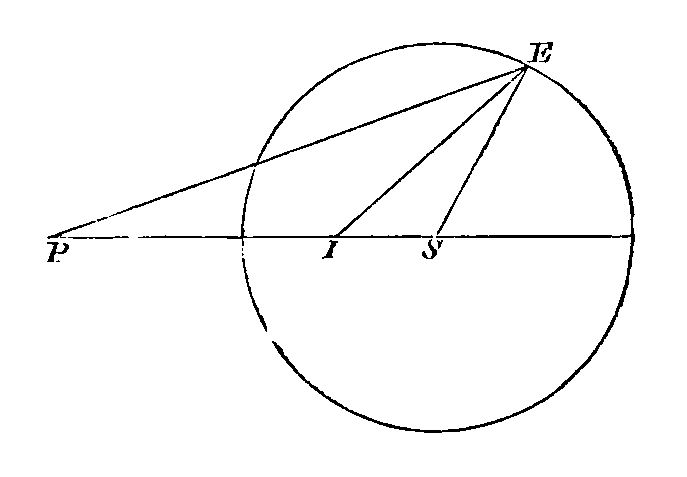
\includegraphics[width=0.6\textwidth]{042.png}
\centering
\end{figure}

As \(cc' = a^2\) the triangles \(PSE\) and \(ESI\) are similar; thus we have
\[
\frac{r'}{r} = \frac{c'}{a}\text{.}
\]

In finding the attraction on the internal particle, we may if
we please suppose the matter to be removed which forms a sphere
having its centre at the internal particle and radius equal to \(a - c'\):
thus the limits of integration become \(r' = a - c'\) and \(r' = a + c'\).

Suppose \(\phi(r) = \xp\dfrac{\mu}{r^n}\); the attraction on the internal particle
\[
= \pi \int y^2 \phi(r') dr' = \pi \mu \int \frac{y^2}{r'^n} dr';
\]
the limits being \(a - c'\) and \(a + c'\). Now put \(\xp\dfrac{rc'}{a}\) for \(r'\); thus we get
\(\pi \mu \xp\left(\dfrac{a}{c'}\right)^{n - 1} \displaystyle\int \xp\dfrac{y^2}{r^n} dr\), and the limits of \(r\) are \(\xp\dfrac{a^2}{c'} - a\) and \(\xp\dfrac{a^2}{c'} + a\), that
is, \(c - a\) and \(c + a\).

Hence the attraction on the internal particle at the distance \(c'\)
from the centre is equal to the product of \(\xp\left(\dfrac{a}{c'}\right)^{n-1}\) into the attraction
on the external particle at the distance \(c\) from the centre.
%%-----File: 043.png-----%%

And
\[
\left(\frac{a}{c'}\right)^{n - 1}=\frac{(cc')^{\tfrac{n - 1}{2}}}{c'^{n - 1}}= \left(\frac{c'}{c} \right)^{\tfrac{1}{2}} \left( \frac{c}{c'}\right)^{\tfrac{n}{2}}\text{.}
\]

This is the result which Newton intended to give. He says
that the attraction on the particle at \(I\) is to the attraction on the
particle at \(P\), in ratione composita ex subduplicatâ ratione
distantiarum a centro \(IS\) et \(PS\), et subduplicatâ ratione virium
centripetarum, in locis illis \(P\) et \(I\), ad centrum tendentium. It
seems to me that instead of \(P\) et \(I\) we ought to read \(I\) et \(P\).

\Section
11. Newton's Propositions 83 and 84 shew briefly that there
would be no difficulty in calculating the attraction of a homogeneous
segment of a sphere on a particle situated on the axis of
the segment.

\Section
12. Newton's Propositions 85, 86, and 87 involve simple
general statements, which need not be repeated here.

Propositions 88 and 89 shew that if the law of attraction is
that of the direct distance, the resultant attraction exerted by a
body or a system of bodies is the same as if the body or system
were collected at its centre of gravity.

\Section
13. Proposition 90 finds the attraction of a circular lamina on
a particle which is situated on the straight line drawn through the
centre of the lamina at right angles to its plane. Then Proposition
91 shews how from this we can deduce the attraction of a
solid of revolution on a particle situated at any point of the axis.
Newton makes this depend on the problem of finding the area of
a certain curve; that is, in modern language, he leaves only a
single integration to be effected. He takes the case of a right
cylinder for an example; and he also states the result for the case
of an ellipsoid of revolution, which he calls a spheroid. He shews
by a special investigation that a shell bounded by two concentric
similar and similarly situated ellipsoidal surfaces of revolution
exerts no attraction on a particle placed at any point within the
hollow part; the demonstration is very striking and well known:
see \textit{Statics}, Chapter \textsc{xiii}. Of course this result includes Newton's
Proposition 70 as a particular case; but the demonstrations differ
and should be carefully compared.
%%-----File: 044.png-----%%

Hence follows the important result that along the same radius
vector from the centre the attraction of an ellipsoid of revolution
on an internal particle varies as the distance from the centre.

Newton contented himself with considering ellipsoids of revolution;
but the processes and results of Proposition 91, as we
now know, may be easily extended to ellipsoids which are not
solids of revolution.

\Section
14. Proposition 92 shews how we may find experimentally the
law of attraction of given matter. Form the given matter into
such a shape that the resultant attraction can be obtained when
the law of attraction is assumed; for example, the shape of a
sphere. Then ascertain by experiment what the resultant attraction
really is at various distances; and thus we shall be guided in
assuming a law of attraction and verifying the assumption.

\Section
15. Proposition 93 treats of the attraction of an infinite plane
lamina, deducing it from Proposition 90. A scholium to this
Proposition gives some interesting remarks relating to the motion
of a particle acted on by a force the direction of which is always
parallel to a fixed straight line.

\Section
16. Newton's Propositions on Attractions are illustrated by a
good commentary in the edition of the \textit{Principia} which is known
as the Jesuits' edition. They had been previously discussed by
Maupertuis, as we shall see in another Chapter. Notes by Plana
on some of the Propositions will be found in the \textit{Memorie della
Reale Accademia \dots\ di Torino}, second series, Vol.\ \textsc{xi.}, 1851.

\Section
17. We pass now to the investigations made by Newton with
respect to the Figure of the Earth; they are contained in Propositions
XVIII., XIX., and XX. of the third Book of the \textit{Principia}:
these Propositions remain substantially the same in the second
and third editions as in the first, but modifications occur arising
from additional information as to the facts involved.

Before we consider these Propositions we ought to advert to
Newton's remarkable conjecture which is contained in Proposition
X. Newton here suggests that the mean density of the Earth may
%%-----File: 045.png-----%%
be five or six times that of water: \dots\ verisimile est quod copia
materiæ totius in Terrâ quasi quintuplo vel sextuplo major sit
quàm si tota ex aqua constaret. We may now consider it certain
that the mean density is between five and six times that of water.
Laplace draws attention to Newton's remarkable conjecture in the
\textit{Connaissance des Tems} for 1823, page 328.

It will be convenient to give the enunciations of Newton's
Propositions XVIII., XIX. and XX.

\begin{squote}
XVIII\@. Axes Planetarum quæ ad eosdem axes normaliter ducuntur
minores esse.

XIX\@. Invenire proportionem axis Planetæ ad diametros eidem
perpendiculares.

XX\@. Invenire et inter se comparare pondera corporum in Terræ
hujus regionibus diversis.
\end{squote}

\Section
18. Proposition XVIII. contains a general statement that the
planets are not accurately spherical. In the first edition Cassini
and Flamsteed are quoted as authorities for this statement with
respect to Jupiter; in the second edition instead of these names
we are referred to astronomers in general.

\Section
19. Proposition XIX. undertakes to determine the ratio of
the axes of a planet. This important process consists of various
steps. In the first edition Newton begins by saying briefly he
finds from calculation that the centrifugal force at the equator is
to the force of attraction there as \(1\) to \(290 \frac{4}{5}\). In the second
edition the details of the calculation are supplied, and the ratio
obtained is that of \(1\) to \(289\): this ratio is that which is now
usually given in our elementary books, and it will be convenient
to adopt it as we proceed with an account of Newton's investigation.

Suppose two slender canals of homogeneous fluid, one along the
polar radius of the earth, and the other along an equatorial
radius. The resultant attraction on the equatorial canal must be
greater than that on the polar canal in the ratio of \(289\) to \(288\) in
order that there may be relative equilibrium. For in proceeding
along any given radius inside the earth the attraction varies as
%%-----File: 046.png-----%%
the distance, and the centrifugal force varies as the distance;
hence the ratio of the latter to the former is constant along the
equatorial radius; so that the effect of the centrifugal force may
be considered equivalent to removing \(\xp\dfrac{1}{289}\) of the force of attraction.

\Section
20. Newton's next step is to compare the attraction of an
oblate ellipsoid of revolution on a particle at its pole with the
attraction of the same body on a particle at its equator, the ellipticity
being supposed very small. He states his results without
giving his process at full. It will be remembered that he had
found an expression for the attraction of an ellipsoid of revolution
at any point of its axis: see Art.\ 13.

I\@. Suppose an oblate ellipsoid of revolution formed from an
ellipse, such that the major semi-axis \(\mathit{CA}\) is to the minor semi-axis
\(CQ\) as \(101\) is to \(100\). The reader can easily draw the diagram
for himself. Newton says that the attraction at \(Q\) would be to the
attraction of a sphere having \(C\) for centre and \(\mathit{CQ}\) for radius, as
\(126\) is to \(125\). If \(\epsilon\) denote the ellipticity we know from our
modern works that this ratio is that of \(1 + \xp\dfrac{4 \epsilon}{5}\) to \(1\); see \textit{Statics},
Chapter \textsc{xiii.}; this agrees closely with Newton's numerical example.

II\@. Suppose a prolate ellipsoid of revolution formed from the
same ellipse. Newton says that the attraction at \(A\) would be to
the attraction of a sphere having \(C\) for centre and \(\mathit{CA}\) for radius,
as \(125\) is to \(126\). If \(\epsilon\) denote the ellipticity we know from our
modern works that this ratio is that of \(1 -\xp\dfrac{4\epsilon}{5}\) to \(1\); see \textit{Statics},
Chapter \textsc{xiii.}: this agrees with Newton's numerical example.

In the first edition Newton put the fraction \(\xp\dfrac{2}{15}\) after \(126\) and
\(125\) in I. and II\@. The fraction was removed by Cotes: see the
\textit{Correspondence of Newton and Cotes}, page 69.

III\@. Now return to the oblate ellipsoid of revolution. Suppose
a particle at \(A\): Newton says that the attraction on it will be a
mean proportional between the attractions of the sphere and of the
%%-----File: 047.png-----%%
prolate ellipsoid of revolution in II\@. We will develop his argument.
Begin with the sphere having \(\mathit{CA}\) for radius; if we change
the radius which lies along \(\mathit{CQ}\) into \(\mathit{CQ}\) we deduce the oblate
ellipsoid of revolution; if in this we change the radius which is at
right angles to \(\mathit{CA}\) and \(\mathit{CQ}\) into a radius equal to \(\mathit{CQ}\), we deduce
the prolate ellipsoid of revolution. Now each of these changes
may be assumed to have affected the attraction to the same
amount; and so the attraction of the oblate ellipsoid of revolution
is approximately an arithmetical mean between the attractions of
the sphere and of the prolate ellipsoid of revolution. Moreover
the arithmetical mean between two nearly equal quantities is
practically equivalent to the geometrical mean. Hence, finally, the
attraction of the sphere with centre \(C\) and radius \(\mathit{CA}\) is to the
attraction of the oblate ellipsoid of revolution on the particle at \(A\)
as \(126\) is to \(125\frac{1}{2}\).

IV\@. Thus we have

Attraction of oblate ellipsoid of revolution at the pole\\
\(=\xxp\dfrac{126}{125}\,\times\) attraction of sphere of radius 100 at its surface;\\
attraction of sphere of radius 101 at its surface\\
\(= \xxp\dfrac{126}{125 \frac{1}{2}}\,\times\) attraction of oblate ellipsoid of revolution at its equator;\\
attraction of sphere of radius 100 at its surface\\
\(= \xxp\dfrac{100}{101}\,\times\) attraction of sphere of radius 101 at its surface.

Hence we find by multiplication that the ratio of the attraction
of the oblate spheroid of revolution at the pole to the attraction at
the equator is expressed by \(\xp\dfrac{126}{125}\times\xp\dfrac{126}{125 \frac{1}{2}}\times\xp\dfrac{100}{101}\), that is, by \(\xp\dfrac{501}{500}\)
nearly.

\Section
21. In future I shall use the single word \textit{oblatum} instead of
oblate ellipsoid of revolution, and the single word \textit{oblongum} instead
of prolate ellipsoid of revolution.

\Section
22. I shall now make some remarks on the statement by
Newton which forms the paragraph III. of Art.\ 20.
%%-----File: 048.png-----%%

If we cut the three solids by two adjacent planes at right
angles to \(AC\) we obtain slices, two of which are circular and the
other elliptical. It is not difficult to believe that in passing from
the larger circular slice to the elliptical slice we diminish the
attraction by the same amount as we do in passing from the
elliptical slice to the smaller circular slice. In fact, the decrement
of mass is about the same in the two cases, and the mass lost is at
about the same situation with respect to the attracted particle in
the two cases.

It is easy to test the statement by the aid of the modern
formula; see \textit{Statics}, Chapter \textsc{xiii}.

First take an oblatum of density unity; let \(r\) be its greatest
radius and \(r \xsurd (1 - e^2)\) its least radius. The attraction at the
equator
\[\begin{aligned}
&= 2 \pi r (1 - e^2) \int_{0}^{\tfrac{\pi}{2}} \sin^3 \theta (1 - e^2 \sin^2 \theta)^{-1} \,d\theta\\
&= \frac{4 \pi r (1 - e^2)}{3}\left\{ 1 + \frac{4}{5} e^2 + \frac{4\ldot6}{5\ldot7} e^4 + \ldots\right\}\text{.}
\end{aligned}\]

Next take an oblongum; let \(r\) be its greatest radius and
\(r \xsurd (1 - e^2)\) its least radius. The attraction at the pole
\[\begin{aligned}
&= 4 \pi r (1 - e^2) \int_{0}^{\tfrac{\pi}{2}} \sin \theta \cos^2 \theta (1 - e^2 \cos^2 \theta)^{-1} \,d\theta\\
&= \frac{4 \pi r (1 - e^2)}{3}\left\{ 1 + \frac{3e^2}{5} + \frac{3e^4}{7} + \ldots \right\}\text{.}
\end{aligned}\]

The attraction of a sphere of radius \(r\) at its surface \(=\xp\dfrac{4 \pi r}{3}\).

Suppose \(e\) so small that we may reject \(e^4\) and higher powers
of \(e\); then the first of these attractions reduces to \(\xxp\dfrac{4 \pi r}{3}\left(1 - \dfrac{e^2}{5}\right)\),
and the second to \(\xxp\dfrac{4 \pi r}{3}\left(1 - \dfrac{2e^2}{5}\right)\), so that the first is an arithmetical
mean between the second and the third. But this statement does
not hold if we carry our approximations as far as \(e^4\) inclusive; it
will be found then that the first of the attractions is rather better
represented by the mean proportional between the second and the
third than by their arithmetical mean.
%%-----File: 049.png-----%%

It will be convenient to quote Newton's own words, premising
that in his diagram \(PCQ\) is the polar diameter and \(ACB\) an
equatorial diameter.

\begin{squote}
Est autem gravitas in loco \(A\) in Terram, media proportionalis inter
gravitates in dictam Sphæroidem et Sphæram, propterea quod Sphæra,
diminuendo diametrum \(PQ\) in ratione \(101\) ad \(100\), vertitur in figuram
Terræ; et hæc figura diminuendo in eadem ratione diametrum tertiam,
quæ diametris duabus \(AB\), \(PQ\) perpendicularis est, vertitur in dictam
Sphæroidem, et gravitas in \(A\), in casu utroque, diminuitur in eadem
ratione quam proximè.
\end{squote}

The words \textit{in eadem ratione}, which occur at the end of this
extract, seem to have been formerly misunderstood; it was supposed
Newton intended to affirm that the attractions of the three
bodies were in the same ratio as their volumes. But this is not
the case. The volume of the oblatum is \(\xp\dfrac{4\pi r^3}{3}\xsurd(1-e^2)\); the
volume of the oblongum is \(\xp\dfrac{4\pi r^3}{3}(1-e^2)\); and the volume of the
sphere is \(\xp\dfrac{4\pi r^3}{3}\): these volumes are not in the ratio of the attractions
exactly nor approximately to the order of \(e^2\). Hence the
following passage, which occurs in a note in the Jesuits' edition of
the \textit{Principia}, is erroneous: ``\dots\ attractiones sphæræ, sphæroidis
compressæ, et sphæroidis oblongatæ, sunt respectivè ut quantitates
materiæ in illis corporibus contentæ quam proximè.''

The words \textit{in eadem ratione}, which occur at the end of the
extract from Newton, must be understood to mean only \textit{to the
same amount}; and must not be taken in exactly the same sense
as in the middle of the passage.

It is obvious, however, that it would have been simpler and
more natural to say, that the attraction of the oblatum is an
\textit{arithmetical mean} between those of the sphere and the oblongum,
than to say that it is a \textit{mean proportional} between them, to the
order of accuracy which Newton adopts.

\Section
23. Newton now compares the resultant attraction on the
fluid in a slender canal having \(AC\) for its axis, with that on the
fluid in a slender canal having \(QC\) for its axis. He finds that
%%-----File: 050.png-----%%
these resultants are in a ratio compounded of the ratios of the
lengths and of the ratios of the attractions at the extremities
\(A\) and \(Q\): see Art.\ 33. Thus the resultant attraction on the fluid
in the canal \(AC\) is to that on the fluid in the canal \(QC\), as
\(101 \times 500\) is to \(100 \times 501\), that is, as \(505\) is to \(501\). Hence
Newton infers, that if the centrifugal force at any point of \(AC\) is
to the attraction at that point as \(4\) is to \(505\), the weights of the
fluids in the two canals will be equal, and the canals in relative
equilibrium.

\Section
24. The last step in the preceding Article is more obvious to
us, who have the modern theory of the equilibrium of fluids, than
it would have been before that theory was constructed. We see
that in the state of relative equilibrium the pressure at \(C\) must be
the same in every direction round \(C\): the pressure on a given
area at right angles to \(AC\) will be measured by the weight of a
column of fluid having that area for its section; and similarly for
the pressure on an area at right angles to \(QC\).

The canals of fluid which Newton considered were rectilinear,
meeting at the centre. Other writers, especially Clairaut, considered
canals of various forms, curvilinear as well as rectilinear,
meeting at any point of the body. The more simple case to
which Newton restricted himself may be conveniently described
as that of \textit{central columns}; so that the word \textit{canal} may be in
future used in Clairaut's more general sense.

\Section
25. It is now necessary to explain carefully the sense in
which the words \textit{attraction}, \textit{gravity} and \textit{weight} will be used in this
history.

By the \textit{attraction} of the Earth at any point, I understand that
force which the Earth would exert, supposing it did not rotate on
its axis. By \textit{gravity} I denote the force which arises from the combination
of the attraction and the so-called \textit{centrifugal force}; and
\textit{weight} may be considered as an effect produced by gravity as the
cause. As we may measure the cause by the effect, it will be
found that it is often indifferent whether we use the word \textit{gravity}
or the word \textit{weight}: but it is convenient to have both words at
our service. The word \textit{weight} is thus left in its ordinary sense
%%-----File: 051.png-----%%
as denoting an effect which is actually produced in the existing
constitution of things, and actually observed.

It would be convenient if we had a word for the effect which
corresponds to \textit{attraction} as a cause; but such a word is not very
often required, because practically we are not concerned with an
Earth at rest, but with one which rotates. For want of such a
word I employ the phrase \textit{resultant attraction} in Arts.\ 19 and 23.

The distinctions which we have here drawn actually exist,
and various modes have been adopted for preventing confusion.
Some writers, indeed, leave us to gather from the context the
sense in which they use their terms. This is the case with
Newton himself. Thus, for instance, in the passage quoted in
Art.\ 22, he uses \textit{gravitas} for what I call \textit{attraction}. In his Proposition
XX. he uses \textit{gravitas} for what I call \textit{gravity}. In his Proposition
XIX. he uses \textit{pondus} sometimes to express the effect produced
by what I call \textit{attraction}, and sometimes in the sense I give
to \textit{weight}. To secure accuracy I have used not his words but
my own.

Maupertuis used \textit{gravité} for my \textit{attraction}, and \textit{pesanteur} for
my \textit{gravity}; and Clairaut followed Maupertuis. See Maupertuis's
\textit{Figure de la Terre}, page 158, and Clairaut's \textit{Figure de la
Terre}, page xiii. In the \textit{Mécanique Céleste}, Vol.\ \textsc{v.}\ page 2, we have
the same use of \textit{gravité}.

Maupertuis had previously used \textit{pesanteur réduite} for my
\textit{gravity}: see the Paris \textit{Mémoires} for 1734, page 97.

Bouguer used \textit{pesanteur primitive} for my \textit{attraction}, and \textit{pesanteur
actuelle} for my \textit{gravity}: see the Paris \textit{Mémoires} for 1734,
page 22, and Bouguer's \textit{Figure de la Terre}, page 169.

Maclaurin used \textit{gravitation} as Maupertuis used \textit{pesanteur},
and \textit{gravity} as Maupertuis used \textit{gravité}: so also did Thomas
Simpson. See Maclaurin's \textit{Fluxions}, page 551, and Simpson's
\textit{Mathematical Dissertations}, page 22. The word \textit{gravitation} has
been employed by some eminent modern writers in about the
same sense as my \textit{attraction}; as, for example, in Airy's article
on \textit{Gravitation} in the \textit{Penny Cyclopædia}, and by Thomson and
Tait in their \textit{Natural Philosophy}, Vol.\ \textsc{i.}\ page 167.
%%-----File: 052.png-----%%

Boscovich used \textit{gravitas primitiva} for my \textit{attraction}, and
\textit{gravitas residua} for my gravity: see his \textit{De Litteraria Expeditione},
page 403. But in the Bologna \textit{Commentarii}, Vol.\ \textsc{iv.}\ page
382, he uses \textit{tota gravitas} for the \textit{gravitas residua} of his book.

In the French translation of Boscovich's book, we have \textit{gravité
primitive} for his \textit{gravitas primitiva}, and \textit{gravité absolue} for his
\textit{gravitas residua}; see the pages 8 and 384 of the translation.

The word \textit{pesanteur} is used by Bailly in his \textit{Histoire de l'Astronomie
Moderne}, Vol.\ \textsc{iii.}\ page 4, as equivalent to my \textit{attraction};
but in general the sense assigned by Maupertuis and Clairaut to
\textit{pesanteur} has been adopted by their successors. In French the
word \textit{poids} is almost equivalent to my \textit{weight}; see Maupertuis's
\textit{Figure de la Terre}, page 155.

\Section
26. We now return to Art.\ 23. The result there obtained is,
that if the ellipticity be \(\xp\dfrac{1}{101}\), then for relative equilibrium the
centrifugal force at the equator must be \(\xp\dfrac{4}{505}\) of the attraction
there. Newton now forms a proportion. He says:

\begin{squote}
Verum vis centrifuga partis cujusque est ad pondus ejusdem ut
1 et 289, hoc est, vis centrifuga, quæ deberet esse ponderis pars
\(\xp\dfrac{4}{505}\), est tantum pars \(\xp\dfrac{1}{289}\). Et propterea dico, secundum Regulam
auream, quod si vis centrifuga \(\xp\dfrac{4}{505}\) faciat ut altitudo aquæ in crure \(ACca\)
superet altitudinem aquæ in crure \(QCcq\) parte centesimâ totius altitudinis:
vis centrifuga \(\xp\dfrac{1}{289}\) faciet ut excessus altitudinis in crure \(ACca\) sit altitudinis
in crure altero \(QCcq\) pars tantum \(\xp\dfrac{1}{229}\).
\end{squote}

These are the numbers of the second and third editions; in
the first edition Newton has \(\xp\dfrac{1}{290}\) instead of \(\xp\dfrac{1}{289}\), and \(\xp\dfrac{3}{689}\) instead
of \(\xp\dfrac{1}{229}\). In his diagram \(ca\) is parallel and adjacent to
\(CA\) and \(cq\) is parallel and adjacent to \(CQ\).
%%-----File: 053.png-----%%

\Section
27. If we put Newton's investigation into a modern form it
will stand thus. Let \(\epsilon\) be the ellipticity, supposed very small;
then the attraction of an oblatum at its pole is to the attraction
of the oblatum at its equator as \(1 + \xp\dfrac{\epsilon}{5}\) is to \(1\); see \textit{Statics}, Chapter
\textsc{xiii}. Hence, as in Art.\ 23, the ratio of the resultant attraction
on the fluid in \(AC\) to the resultant attraction on the fluid in \(QC\)
is expressed by \(\xp\dfrac{1 + \epsilon}{1 + \mystrut(2.6,1.8)\dfrac{\epsilon}{5}}\), that is, by \(1 + \xp\dfrac{4\epsilon}{5}\) approximately. Therefore
for relative equilibrium we must have the centrifugal force
at any point in \(AC\) equal to \(\xp\dfrac{4\epsilon}{5}\) of the attraction at that point.

Newton, in fact, sees that the fraction which we have found
to be \(\xp\dfrac{4\epsilon}{5}\) must be proportional to \(\epsilon\); hence it may be denoted
by \(k\epsilon\), where \(k\) is some constant. Then, when \(\epsilon = \xp\dfrac{1}{101}\), he finds
that \(k \epsilon = \xp\dfrac{4}{505}\), so that \(k = \xp\dfrac{404}{505} = \dfrac{4}{5}\).

\Section
28. The result obtained by Newton then is that if the Earth
is homogeneous and its shape the same as if it were entirely fluid,
the ellipticity must be \(\xp\dfrac{1}{230}\), supposing it to be very small; that is,
the ellipticity must be \(\xp\dfrac{5}{4}\) of the ratio of the centrifugal force to the
attraction at the equator. The result is very important in the
theory of the subject; but we know now that the ellipticity is about
\(\xp\dfrac{1}{300}\), and we are confident that the Earth is not homogeneous.

\Section
29. Newton proceeds to some remarks on the oblateness of
Jupiter.

Let \(j\) denote the ratio of the centrifugal force to the attraction
at the equator, and \(\epsilon\) the ellipticity; then we have shewn that
\(j = \xp\dfrac{4\epsilon}{5}\).
%%-----File: 054.png-----%%

In his first edition Newton erroneously asserts that \(j\) is independent
of the density. He says:

\begin{squote}
Si Planeta vel major sit vel densior, minorve aut rarior quàm Terra,
manente tempore periodico revolutionis diurnæ, manebit proportio vis
centrifugæ ad gravitatem, et propterea manebit etiam proportio diametri
inter polos ad diametrum secundum æquatorem.
\end{squote}

Accordingly he considers \(j\) to vary inversely as the square of
the time of rotation; so that the value of \(j\) for Jupiter becomes
\(\xp\dfrac{29}{5}\) times its value for the Earth: and hence Jupiter's ellipticity
is taken to be \(\xp\dfrac{29}{5}\) times that of the Earth, so that the ratio of the
difference of the axes to the minor axis is about \(\xp\dfrac{1}{39\frac{3}{5}}\).

In the second edition Newton corrects his error. He says:

\begin{squote}
Si Planeta major sit vel minor quàm Terra manente ejus densitate
ac tempore periodico revolutionis diurnæ, manebit proportio vis centrifugæ
ad gravitatem\dots.
\end{squote}

Accordingly he now rightly considers \(j\) to vary inversely as
the density as well as inversely as the square of the time of
rotation; so that, taking the density of Jupiter to be \(\xp\dfrac{1}{5}\) of the
density of the Earth, the ratio of the difference of the axes to the
minor axis becomes \(\xp\dfrac{29}{5} \times \xp\dfrac{5}{1} \times\xp\dfrac{1}{229}\), that is, about \(\xp\dfrac{1}{8}\).

In the third edition, the density of Jupiter is taken as \(\xp\dfrac{94\frac{1}{2}}{400}\) of
the density of the Earth; and the ratio of the difference of the
axes to the minor axis becomes about \(\xp\dfrac{1}{9\frac{ 1}{5}}\).

\Section
30. In the first and second editions these words occur at the
end of Proposition XIX.:

\begin{squote}
Hæc ita se habent ex Hypothesi quod uniformis sit Planetarum
materia. Nam si materia densior sit ad centrum quàm ad circumferentiam,
diameter, quæ ab oriente in occidentem ducitur, erit adhuc major.
\end{squote}
%%-----File: 055.png-----%%

Thus Newton considered that if the Earth, instead of being
of uniform density, were denser towards the centre than towards
the surface, the ellipticity would be increased; see also Art.\ 37.
But Newton was wrong. Assuming the original fluidity of the
Earth, the ellipticity is diminished by increasing the density of
the central part, supposed spherical, and making it solid. This
was shewn by Clairaut, who pointed out Newton's error: see
Clairaut's \textit{Figure de la Terre}, pages 157, 223, 224, 253\dots 256.
Clairaut, however, ought to have remarked that Newton omitted
the passage in his third edition.

In his third edition, as I have just said, Newton omitted the
above passage. He says instead:

\begin{squote}
Hoc ita se habet ex hypothesi quod corpus Jovis sit uniformiter
densum. At si corpus ejus sit densius versùs planum æquatoris quàm
versùs polos, diametri ejus possunt esse ad invicem ut 12 ad 11, vel 13
ad 12, vel forte 14 ad 13.
\end{squote}

Then, after stating some observations as to the ratio of the
axes of Jupiter, Newton says:

\begin{squote}
Congruit igitur theoria cum phænomenis. Nam planetæ magis incalescunt
ad lucem Solis versùs æquatores suos, et propterea paulo magis
ibi decoquuntur quàm versùs polos.
\end{squote}

It might then appear that in his third edition Newton had
recognised his error; but we shall find, when we discuss Proposition
XX., that a distinct trace of the error still remains: see
Arts.\ 38 and 41.

\Section
31. I do not feel certain as to the meaning of the sentence
``congruit \dots\ polos,'' which I have quoted in the preceding Article.
Since heat expands bodies it would appear that the equatorial
parts ought by the Sun's action to be rendered \textit{less} dense than
the polar parts. The same difficulty presented itself to Boscovich:
see page 475 of his \textit{De Litteraria Expeditione}, and pages
89 and 380 of Stay's \textit{Philosophiæ Recentioris}, Vol.\ \textsc{ii.}\ Clairaut
says in his \textit{Figure de la Terre}, pages 223, 224:

\begin{squote}
De la même manière, on voit combien il était inutile à M. Newton,
lorsque sa théorie lui donnait pour Jupiter, une ellipticité moindre que
%%-----File: 056.png-----%%
celle qui résulte des observations, d'aller imaginer que l'équateur de
cette planète étant continuellement exposé aux ardeurs du soleil, était
plus dense que le reste de la planète. Il n'avait qu'à supposer simplement
que le noyau était plus dense que le reste de la planète\dots.
\end{squote}

The word \textit{moindre} in this passage is wrong; for Newton's
theoretical value of Jupiter's ellipticity in the third edition is
\textit{greater} than the value in the observations he quotes.

\Section
32. I will now briefly indicate the changes which Newton's
Proposition XIX. underwent in the later editions with respect to
the facts which it involves.

In the first edition, Newton takes the mean semi-diameter of
the Earth to be 19615800 Paris feet, \textit{juxta nuperam Gallorum mensuram:}
this alludes to Picard's measurement of the length of an
arc of the meridian in France.

In the second edition, Newton refers to the measurements
made by Picard, by Norwood, and by Cassini; according to
Cassini's measurement, the semi-diameter is 19695539 Paris feet,
supposing the Earth spherical. This Cassini is the first of the distinguished
family; his name was Jean Dominique Cassini, but he
is often called simply Dominique Cassini.

In the third edition, Newton refers also to the measurement
made by the son of Dominique Cassini, who is known as Jacques
Cassini. Picard had obtained 57060 toises for the length of a
degree; the arc measured by D. and J. Cassini gave 57061
toises for the mean length of a degree. We shall see as we proceed
with the history that these measurements were subsequently
re-examined and corrected.

\Section
33. We now come to Newton's Proposition XX., the object of
which is to compare the weights of a given body at different
places on the Earth's surface.

Newton begins with an important result, which is deduced
from his principle of balancing columns: see Art.\ 23. At any
point of the Earth's surface, let \(f\) denote the force of gravity,
\textit{resolved along the radius}; let \(r\) be the distance of this point from
%%-----File: 057.png-----%%
the centre; let \(x\) be the distance from the centre of any point on
the same radius: then the force of gravity at this point \textit{resolved
along the radius} will be \(\xp\dfrac{fx}{r}\), because along the same radius within
the Earth both the resolved attraction and the resolved centrifugal
force vary as the distance. Hence the resolved weight
of a column of fluid extending from the surface to the centre, is
measured by \(f \displaystyle\int_0^r \xp\dfrac{ x }{ r} dx\), that is, by \(\xp\dfrac{1}{2} fr\). And as the resolved
weight of every column must be the same, for relative equilibrium,
we must have \(fr\) constant, and so \(f\) must vary inversely as \(r\).

This is equivalent to an expansion of Newton's brief outline:
it becomes more obvious to modern readers by the aid of the
theory of the equilibrium of fluids. It is clear that the final
result would be true if the resolved force within the Earth varied
as \textit{any} direct power of the distance instead of as the \textit{first} power.

Thus we may say that the weight of a given body at any point
of the Earth's surface \textit{when resolved along the radius} varies inversely
as the radius. Newton, however, omits the words which I have
printed in Italics. Since the Earth is very nearly a sphere, the
omission will be of no consequence practically, but theoretically it
is important to be accurate.

\Section
34. Newton proceeds thus:

\begin{squote}
Unde tale confit Theorema, quod incrementum ponderis, pergendo
ab Æquatore ad Polos, sit quam proximè ut Sinus versus
latitudinis duplicatæ, vel quod perinde est ut quadratum Sinus recti
Latitudinis.
\end{squote}

The result here stated may be thus investigated. Let \(g\) denote
the weight of a given body at any point of the Earth's surface;
let \(r\) denote the radius at that point, and \(\phi\) the angle which the
normal at that point makes with the radius. Then, \textit{assuming that
the direction of gravity coincides with the normal}, the resolved part
of the weight along the radius will be \(g \cos \phi\). Therefore, by
Art.\ 33, we have \(g \cos \phi =\xp\dfrac{ \lambda}{ r}\), where \(\lambda\) is some constant, so that
%%-----File: 058.png-----%%
\(g = \xp\dfrac{\lambda}{r \cos \phi}\). Let \(G\) denote the weight of the given body at the
equator, \(a\) the radius of the equator; then
\[
g - G = \lambda \left( \frac{1}{r \cos \phi} - \frac{1}{a} \right)\text{.}
\]

By neglecting powers of the ellipticity beyond the first, it is
found that \(\xp\dfrac{1}{r \cos \phi} - \xp\dfrac{1}{a}\) varies as the square of the sine of the
latitude.

The words printed in Italics in the above investigation involve
a principle which is familiar to us in the modern theory of fluids;
as we shall see hereafter, this principle was used by Huygens.
Newton, however, tacitly assumes that the direction of gravity
coincides with the radius. It is true, that to the order of approximation
which we adopt \(\cos \phi\) may be put equal to unity, and so
there is no practical error involved in Newton's assumption: but
theoretically his investigation of the very important proposition
now before us is thus rendered obscure and imperfect.

\Section
35. In Newton's second and third editions, we have after the
passage last quoted these words: ``Et in eadem circiter ratione
augentur arcus graduum Latitudinis in Meridiano.'' This is a fact
in the theory of the Conic Sections with which we are now
familiar. Let \(p\) denote the perpendicular from the centre of
an ellipse on the tangent at any point; then the radius of curvature
varies as \(\xp\dfrac{1}{p^3}\). Thus the increase of the radius of curvature
in proceeding from the equator towards the pole varies as \(\xp\dfrac{1}{p^3} - \xp\dfrac{1}{a^3}\);
and by neglecting powers of the ellipticity beyond the first it is
found that this varies as the square of the sine of the latitude.

\Section
36. In the first edition Newton calculated the relative weights
of a given body at Paris, Goree, Cayenne, and the Equator.
As observations of the length of a seconds pendulum had been
made at Paris, Goree, and Cayenne, the relative weights of a body
at those places were known, and thus a test of the accuracy of the
theory was furnished.
%%-----File: 059.png-----%%

\Section
37. The following sentences occur in the first edition; they
are repeated substantially in the second edition, but are omitted
in the third edition.

\begin{squote}
Hæc omnia ita se habebunt, ex Hypothesi quod Terra ex uniformi
materia constat. Nam si materia ad centrum paulò densior sit quàm
ad superficiem, excessus illi erunt paulò majores; propterea quod, si
materia ad centrum redundans, qua densitas ibi major redditur, subducatur
et seorsim spectetur, gravitas in Terram reliquam uniformiter
densam erit reciprocè ut distantia ponderis à centro; in materiam verò
redundantem reciprocè ut quadratum distantiæ à materia illa quam
proximè. Gravitas igitur sub æquatore minor erit in materiam illam
redundantem quàm pro computo superiore, et propterea Terra ibi
propter defectum gravitatis paulò altius ascendet quàm in precedentibus
definitum est.
\end{squote}

The preceding sentences contain a portion of truth. Suppose
that a mass of rotatory homogeneous fluid has taken the form
which Newton assigns for relative equilibrium. Then gravity
at the pole is to gravity at the equator, inversely as the corresponding
distances from the centre; and if we suppose the oblatum
to become solid, this ratio is not changed. Next suppose
that the central part is made denser than the rest, this central
part being spherical in shape. Thus the gravity is increased both
at the pole and at the equator; but the additional gravity at the
pole is to that at the equator inversely as the squares of the
corresponding distances. Therefore the whole gravity at the
equator bears to the whole gravity at the pole a \textit{less} ratio than
for the case of the homogeneous body.

But now Newton in some way returns, as it were, to the supposition
of fluidity. It is not obvious whether the whole mass
is supposed to be fluid, or whether the central spherical part is
still left solid. In either case a new investigation would have to
be supplied, in order to determine the figure of the fluid part
for relative equilibrium; and no use could be made of a result
obtained from the balancing at the centre of \textit{homogeneous} columns.
As we have said in Art.\ 30, the investigations of Clairaut bring
out the ellipticity \textit{less} than for the homogeneous case, and not
\textit{greater} as Newton stated.
%%-----File: 060.png-----%%

According to Clairaut, Newton's error lay in thinking that
gravity at the ends of the columns must be inversely proportional
to the lengths of the columns for relative equilibrium, whether
the fluid is homogeneous or not. See Clairaut's \textit{Figure de la
Terre}, pages 224 and 256, and Stay's \textit{Philosophiæ Recentioris},
Vol.\ \textsc{ii.}\ page 370.

\Section
38. In the first edition, as we have stated, Newton referred
to pendulum observations at only three places, Paris, Goree, and
Cayenne. These observations indicated a rather greater variation
in the length of the seconds pendulum than the theory
suggested. So Newton says:

\begin{squote}
\dots\ et propterea (si crassis hisce Observationibus satìs confidendum
sit) Terra aliquanto altior erit sub æquatore quàm pro superiore
calculo, et densior ad centrum quàm in fodinis prope superficiem.
\end{squote}

He then points out the advantage which would be derived
from a set of experiments for determining the relative weights
of a given body at various places on the Earth's surface.

\Section
39. In the second edition Newton gave a table of the lengths
of a degree of the meridian and of the lengths of the seconds
pendulum in different latitudes. This table was computed by
the aid of his theory, taking from observation the length of a
degree of the meridian in the latitude of Paris, and also the
length of the seconds pendulum there. The table is repeated
in the third edition; but the lengths of the degrees are not
the same as in the second edition. The lengths are expressed
in toises; at the equator, at \(45°\), and at the pole, the lengths are
respectively \(56909\), \(57283\), and \(57657\) in the second edition;
while in the third edition they are \(56637\), \(57010\), and \(57382\):
the difference is, of course, owing to the adoption of a fresh result
from the measurement in France. After the table in the second
edition we have these words:

\begin{squote}
Constat autem per hanc Tabulam, quod graduum inæqualitas tam
parva sit, ut in rebus Geographicis figura Terræ pro Sphærica haberi
possit, quodque inæqualitas diametrorum Terræ facilius et certius per
%%-----File: 061.png-----%%
experimenta pendulorum deprehendi possit vel etiam per Eclipses Lunæ,
quam per arcus Geographice mensuratos in Meridiano.
\end{squote}

I cannot understand how the ratio of the axes could be found
by pendulum experiments or by eclipses better than by measured
arcs. In the third edition the words which follow ``haberi possit''
are omitted, and instead of them we have ``præsertim si Terra
paulò densior sit versùs planum æquatoris quàm versùs polos.''

\Section
40. In the second and third editions Newton referred to many
more pendulum observations than in the first edition. We see
from pages 69\dots 89 of the \textit{Correspondence of Newton and Cotes},
that the arrangement of this part of the work for the second
edition was a matter of some trouble. The figures in the final
draft of Newton were corrected by Cotes: compare pages 85 and
92 of the \textit{Correspondence} with the second edition of the \textit{Principia}.
The facts are stated nearly in the same terms in the
second and third editions.

\Section
41. The more numerous observations to which Newton could
now appeal, concurred with the smaller number before used, in
giving a greater variation to the length of the seconds pendulum
than theory suggested. Accordingly, the sentence which we
quoted in Art.\ 38, appears in the second and third editions,
omitting the words \textit{si crassis \dots\ sit}. Newton adds, however, ``nisi
forte calores in Zona torrida longitudinem Pendulorum aliquantulum
auxerint.''

The supposition that the pendulum observations required a
greater ellipticity than \(\xp\dfrac{1}{230}\) was shewn to be untenable by Clairaut:
see his \textit{Figure de la Terre}, page 252.

\Section
42. In the second edition Newton seems to come to the
conclusion that we should correct the theory by observation, and
thus take \(31 \frac{7}{12}\) miles as the excess of the equatorial semi-diameter
over the polar semi-diameter. In the third edition, however, he
seems to consider that we may hold to the value, \(17\) miles, furnished
by theory.

\Section
43. In the second edition Proposition XX. ends with a paragraph
in which Newton adverts to the hypothesis, founded on
%%-----File: 062.png-----%%
some measurements by Cassini, that the Earth is an oblongum:
Newton deduces results from this hypothesis which are contrary
to observations. The paragraph does not appear in the third
edition, although the oblong form continued to find advocates for
some years after the death of Newton.

\Section
44. Newton's investigations in the theories of Attraction and
of the Figure of the Earth may justly be considered worthy of his
great name. The propositions on Attraction are numerous,
exact, and beautiful; they reveal his ample mathematical power.
The treatment of the Figure of the Earth is, however, still more
striking; inasmuch as the successful solution of a difficult problem
in natural philosophy is much rarer than profound researches in
abstract mathematics. Newton's solution was not perfect; but it
was a bold outline, in the main correct, which succeeding investigators
have filled up but have not cancelled. Newton did not
demonstrate that an oblatum is a possible form of relative equilibrium;
but, assuming it to be such, he calculated the ratio of
the axes. This assumption may be called Newton's \textit{postulate}
with respect to the Figure of the Earth: the defect thus existing
in his process was supplied about fifty years later by Stirling
and Clairaut. The difficulty arose from the imperfect state of the
theory of fluid equilibrium, which undoubtedly must have produced
many obstacles for the earliest investigators in mixed
mathematics. Clairaut subsequently gave methods which are
sound and satisfactory to a reader who can translate them into
modern language; but even these may have appeared obscure to
Clairaut's contemporaries. Euler, in the Berlin \textit{Mémoires} for
1755, first rendered Hydrostatics easily intelligible by introducing
a symbol \(p\) to measure the pressure at any point of a fluid.

\Section
45. Besides the defect in Newton's theory which we have
pointed out, Laplace finds another, saying in the \textit{Mécanique
Céleste}, Vol.\ \textsc{v.}\ page 5, ``Il suppose encore, sans démonstration,
que la pesanteur à la surface, augmente de l'équateur aux pôles,
comme le carré du sinus de la latitude.'' But Laplace is not
right. Newton did not absolutely assume the proposition; he
gave a demonstration though it was imperfect; see Art.\ 34.
%%-----File: 063.png-----%%
Laplace's language is inaccurate moreover; it is \textit{not gravity} that
increases as the square of the sine of the latitude, but the \textit{variation
in gravity}. Laplace proceeds to observe that Newton regarded
the Earth as homogeneous, while observations prove
incontestably that the densities of the strata increase from the
surface to the centre. Laplace's language could scarcely be
stronger if borings had actually been executed from the surface
to the centre, and had thus rendered the strata open to inspection.
He means, of course, that by combining observations made
at various places on the surface of the Earth with the suggestions
of theory, we are led to infer that the density increases from
the surface to the centre. See the \textit{Mécanique Céleste}, Vol.\ \textsc{v.}\ page 12.

Laplace truly says that, notwithstanding the imperfections,
the first step thus made by Newton in the theory must appear
immense.

\Section
46. A notice of the \textit{Principia} was given in the \textit{Philosophical
Transactions}, Vol.\ \textsc{xvi.}\ 1687, I presume by Halley, who was then
Secretary of the Society; the simple but expressive words we find
on page 297 are still as applicable as they were then:

\begin{squote}
\dots\ and it may be justly said, that so many and so Valuable
Philosophical Truths, as are herein discovered and put past dispute,
were never yet owing to the Capacity and Industry of any one Man.
\end{squote}
%%-----File: 064.png-----%%
\Chapter{CHAPTER II.}
\Subhead{HUYGENS.}
\Runhead{\textsc{huygens.}}

\Section
47. \textsc{We} have now to examine an essay by Huygens entitled
\textit{Discours de la Cause de la Pesanteur.}

A small quarto volume was published at Leyden, in 1690,
entitled \textit{Traité de la Lumiere \dots\ Par C.H.D.Z. Avec un Discours
de la Cause de la Pesanteur.} The letters C.H.D.Z. stand for
Christian Huygens de Zulichem.

The volume consists of two parts. Pages 1\dots 124 relate to
Light; they are preceded by a Preface, and a Table of Contents,
on 6 pages, which belong to this part of the volume. After page
124 is a Title-leaf for the part relating to Weight; then a preface
on pages 125\dots 128; then a leaf containing a Table of Contents;
and then the text on pages 129\dots 180.

\Section
48. We of course pass over the part relating to Light, merely
remarking that it is memorable as laying the foundation of the
Undulatory Theory.

The part relating to Weight is said to appear in a Latin version
in the \textit{Opera Reliqua} of Huygens: hence it is sometimes cited
by a Latin title, \textit{De causa gravitatis}, or \textit{De vi gravitatis}. My
references will all be made to the original edition in French, published
during the author's lifetime.

\Section
49. The last paragraph of the Preface gives information as
to the date of composition:

\begin{squote}
La plus grande partie de ce Discours a esté écrite du temps que je
demeurois à Paris, et elle est dans les Registres de l'Academie Royale
%%-----File: 065.png-----%%
des Sciences, jusques à l'endroit où il est parlé de l'alteration des Pendules
par le mouvement de la Terre. Le reste a esté adjouté plusieurs
années apres: et en suite encore l'Addition, à l'occasion qu'on y trouvera
indiquée au commencement.
\end{squote}

The former part of the Discourse, which we are here told had
been written many years since, is of no value.

\Section
50. The theory of Huygens to account for Weight is expounded
on pages 129\dots 144 of the work; we may say briefly
that this theory is utterly worthless. Huygens assumes the existence
of a very rare medium moving about the Earth with
great velocity, not always in the same direction. This rare matter
is surrounded by other bodies, and so prevented from escaping;
and it pushes towards the Earth any bodies which it meets. This
vortex has passed away, as well as those similar but more famous
delusions with which the name of Des Cartes is connected.

\Section
51. Two incidental matters of some interest may be noticed.

On his page 138, Huygens says that there is an invisible ponderable
matter present even in the space from which air has been
exhausted: so that it would appear he took the partial exhaustion
produced by an air-pump for complete exhaustion.

On his page 141, he starts a difficulty which we now know has
been removed by experiments:

\begin{squote}
\dots\ De plus, en portant un corps pesant au fond d'un puits, ou dans
quelque carriere ou mine profonde, il y devroit perdre beaucoup de sa
pesanteur. Mais on n'a pas trouvé, que je scache, par experience qu'il
en perde quoy que ce soit.
\end{squote}

\Section
52. The really valuable part of the Discourse commences on
page 145. Huygens says that at Cayenne the seconds pendulum
had been found to be shorter than at Paris. As soon as he heard
this, he attributed it to the rotation of the Earth. Accordingly
he gives a very good explanation; assuming that there is at the
surface of the Earth a force of constant magnitude directed towards
the centre, and that there is also a centrifugal force. He
shews by calculation, that the centrifugal force at the equator
%%-----File: 066.png-----%%
is about \(\xp\dfrac{1}{289}\) of the central force. He calculates that the seconds
pendulum at Cayenne should be \(\xp\dfrac{5}{6}\) of a line shorter than at Paris;
Richer made it \(1 \frac{1}{4}\) lines shorter by observation.

Huygens calculates that the plumb-line at Paris deviates
nearly \(6\) minutes from the position it would take if there were no
centrifugal force.

\Section
53. On his page 152, Huygens states a principle which has
since generally been called by his name; he says the surface of
the sea is such that at every point the \textit{direction of the plumb-line
is perpendicular to the surface}. The principle may be stated more
generally thus: the direction of the resultant force at any point
of the free surface of a fluid in equilibrium must be normal to the
surface at that point.

\Section
54. On page 152, we arrive at the \textit{Addition} to which
Huygens referred in his preface: see Art.\ 49. His attention was
turned to the subject again by examining an account of some
more pendulum experiments, and by reading Newton's \textit{Principia}.
Huygens first calculates the ratio of the axes of the Earth. He
adopts Newton's principle of the balancing of the polar and equatorial
columns; but retains his own hypothesis, that the attractive
force is central and constant at all distances. Thus he makes the
ratio of the axes to be that of \(577\) to \(578\).

\Section
55. Huygens next finds the equation to the generating curve
of the Earth's surface. He considers it difficult to use his own
principle of the plumb-line, stated in Art.\ 53; and so he uses the
principle of balancing columns. He extends this principle beyond
the application which Newton made of it: see Art.\ 24. Huygens
contemplates canals of various forms, not necessarily passing through
the centre. He says on his page 156: ``et mesme, cela doit arriver
de quelque maniere qu'on conçoive que le canal soit fait, pourvû
qu'il aboutisse de part et d'autre à la surface.''

Let the constant force be denoted by \(\lambda\), the angular velocity
by \(\omega\), and the equatorial radius by \(a\); take the axis of \(x\) to coincide
%%-----File: 067.png-----%%
with the polar diameter, and the axis of \(y\) with an equatorial
diameter. Then, by modern methods, we find for the equation
to the curve which by revolution generates the surface of the
Earth
\[
\lambda\xsurd \left(x^2 + y^2\right) - \frac{\omega^2 y^2}{2} = \lambda a - \frac{\omega^2 a^2}{2} \tag{1}\text{.}
\]
This coincides with Huygens's result.

We may deduce the ratio of the axes from (1); we shall thus
get the same value as Huygens obtained before he investigated
the equation to the curve.

Put \(y = 0\) in (1), thus: \(x = a \xp\left(1 - \dfrac{\omega^2 a}{2\lambda}\right)\); therefore the ratio of
the axes is that of \(1 - \xp\dfrac{1}{2 \times 289}\) to \(1\), that is, the ratio of \(577\) to \(578\).

If \(\epsilon\) and \(j\) have the same meaning as in Art.\ 29, we see that
Huygens's result may be expressed thus: \(\epsilon = \xp\dfrac{j}{2}\).

\Section
56. Huygens says on his page 159, that even if we do not
suppose the central force to be constant, his result remains almost
unchanged. It is important to demonstrate this: and we shall
accordingly shew that the result is approximately true, whatever
may be the law of the force, which is assumed to be central.

Let \(\phi (r)\) denote the force at the distance \(r\) from the centre.
Then, by modern methods, we find for the equation to the generating
curve
\[
\int\phi (r)dr - \frac{\omega^2 y^2}{2} = \text{constant.}
\]

Let \(a\) denote the equatorial radius, and \(b\) the polar. By
putting \(y = 0\), we determine the value of the constant, and the
equation becomes
\[
\int_{0}^{r} \phi (r)dr - \frac{\omega^2 y^2}{2} = \int_{0}^{b} \phi (r)dr\text{.}
\]

Now put \(y = a\); thus
\[
\int_{0}^{a} \phi (r)dr - \frac{\omega^2 a^2}{2} = \int_{0}^{b} \phi (r)dr\text{:}
\]
%%-----File: 068.png-----%%
this is an analytical expression of Newton's principle of the
balancing of central columns. We may put the expression in the
form
\[\int_b^a \phi(r)dr = \frac{\omega^2 a^2}{2}.\]

If \(a - b\) is very small this gives approximately
\begin{gather*}
(a - b)\phi(a) = \frac{\omega^2 a^2}{2},\\
\shortintertext{thus}
\frac{a - b}{a} = \frac{1}{2} \frac{a\omega^2}{\phi(a)},\\
\shortintertext{that is}
\epsilon = \frac{j}{2}\text{.}
\end{gather*}

Moreover, we can shew that the diminution of the radius
in passing from the equator to the pole will vary approximately
as the square of the sine of the latitude. For we have
\begin{gather*}
\int^r_0 \phi (r)dr - \frac{\omega^2 y^2}{2} = \int^b_0 \phi (r)dr,\\
\shortintertext{that is}
\int^r_0 \phi (r)dr - \frac{\omega^2 y^2}{2} = \int^a_0 \phi (r)dr - \frac{\omega^2 a^2}{2},\\
\shortintertext{therefore}
\int^a_r \phi (r)dr = \frac{\omega^2}{2} (a^2 - y^2)\text{.}
\end{gather*}

Hence if \(a - r\) be small, we have approximately
\[
(a - r)\phi(a) = \frac{\omega^2}{2} (a^2 - y^2)\text{.}
\]

Thus \(a - r\) varies as \(1 - \xp\dfrac{y^2}{a^2}\), that is, approximately as the
square of the sine of the latitude.

\Section
57. The particular case in which the central force varies
inversely as the square of the distance deserves to be noticed
%%-----File: 069.png-----%%
specially. In this case instead of equation (1) of Art.\ 55 we
obtain
\[\frac{\mu}{\xsurd(x^2+y^2)} +\frac{ \omega^2 y^2}{2} =\frac{ \mu}{a} +\frac{ \omega^2 a^2}{ 2} \tag{2},\]
where \(\xp\dfrac{\mu}{r^2}\) represents the central force.

Put \(y = 0\), then \(x =\xp\dfrac{ a}{ 1 +\mystrut(3.4, 0)\dfrac{ \omega^2 a^3}{2\mu}}\).

Thus the ratio of the axes is that of 1 to \(1 +\xp\dfrac{ \omega^2 a^3}{2\mu}\), and, taking
\(\xp\dfrac{1}{289}\) for \(a\omega^2 \div \xp\dfrac{\mu}{a^2}\), this ratio becomes that of 578 to 579, which is
almost identical with that obtained in Art.\ 54.

\Section
58. If \({\omega^2 a = \lambda}\), the equation (1) of Art.\ 55 is equivalent to
\({y^2 - a^2 = \pm 2ax}\), giving two parabolas, as Huygens observes. He
seems in consequence to accept without hesitation, for relative
equilibrium, a figure of revolution in which the two parts meet so
as to produce an abrupt change of direction: see his page 157.

\Section
59. In his pages 159\dots 168 Huygens makes some interesting
remarks on various points in Newton's \textit{Principia}. Huygens does
not admit that all particles of matter attract each other, but he
does admit a resultant force exerted by the Sun or by a Planet,
and varying inversely as the square of the distance from the centre
of the body. He states that he himself had not extended the
action of \textit{pesanteur} so far as from the Sun to the Planets, nor had
he thought of the law of the inverse square: he fully recognises
Newton's merits as to these points.

\Section
60. We must notice the value he obtained for the increase of
gravity in proceeding from the equator to the pole. He adopts
the ratio of the axes which he had found for the case of a constant
force, and assumes that it will hold when the central force varies
inversely as the square of the distance. Hence since the polar
radius is \(\xp\dfrac{1}{578}\) part shorter than the equatorial radius, gravity
%%-----File: 070.png-----%%
increases by \(\xp\dfrac{1}{289}\) part in passing from the equator to the pole.
And by reason of the absence of centrifugal force at the pole there
is another increase of \(\xp\dfrac{1}{289}\) part. Thus on the whole there is an
increase of \(\xp\dfrac{2}{289}\). He thinks that observation does not confirm this
large increase.

We know now that the increase is not so large as Huygens
made it. His error arises from his assuming that the Earth's
attraction is a single central force varying inversely as the square
of the distance from the centre, instead of calculating the value of
it from the form of the Earth.

\Section
61. Huygens expresses himself as much pleased with Newton's
method of comparing the attraction at the surfaces of the Earth,
the Sun, Jupiter and Mars: see his page 167. Huygens alludes
to the very different estimates which had been made of the Sun's
distance from the Earth: Newton took this to be 5000 times the
Earth's diameter, Cassini to be 10000 times; Huygens himself had
taken it to be 12000 times.

\Section
62. Huygens also refers with pleasure to the researches of
Newton respecting the motion of projectiles in a resisting medium.
Huygens says he had himself formerly investigated this subject,
assuming the resistance to vary as the velocity; after he had
finished his investigations he learned from the experiments made
by the Academy of Sciences at Paris that the resistance in air and
in water varied as the square of the velocity.

He here gives the results of his original investigations without
the demonstrations: see his pages 170\dots 172. It will furnish a
good exercise for students to verify these results, which must have
been obtained with some difficulty in the early days of the
Integral Calculus. The results will be found to be all correct,
except that on the middle of page 171 we ought to read \textit{terminal
velocity} instead of \textit{velocity with which the ground is reached}. The
phrase \textit{terminal velocity} is due to Huygens; see his page 170.
Huygens makes a few remarks on motion in a medium where the
%%-----File: 071.png-----%%
resistance varies as the square of the velocity; but he considers
only a particular case of vertical motion, and a particular case of
oblique motion. The general problem, he truly says, is very
difficult if not impossible.

\Section
63. Huygens finishes with a statement of properties of the
exponential or logarithmic curve; he does not give demonstrations,
but they can be easily supplied.

\Section
64. On the whole we may say that the chief contribution of
Huygens to our subject is the important principle of fluid equilibrium,
which we have noticed in Art.\ 53. He also first solved a
problem in which the form of the surface of a fluid in relative
equilibrium under a given force was accurately determined; see
Art.\ 55. The result has become permanently connected with our
history for a reason which we will now explain.

The assumption that the attraction of the Earth varies inversely
as the square of the distance from a fixed point is equivalent to the
hypothesis that the density of the Earth is infinite towards the
centre. This remark is in fact due to Clairaut; see the \textit{Philosophical
Transactions}, Vol.\ \textsc{xl}.\ page 297. It is sometimes ascribed
to Huygens himself; as in Barlow's \textit{Mathematical Dictionary},
article \textit{Earth}. But, as we have seen, Huygens preferred to consider
the attractive force as \textit{constant}; and this is very different from the
notion involved in Clairaut's remark. Laplace is not quite accurate
in the \textit{Mécanique Céleste}, Vol.\ \textsc{v}.\ page 5, where he omits all notice
of the constant force, and says that Huygens supposed the force to
vary inversely as the square of the distance from a point.

\Section
65. An important error has been sometimes made by representing
the researches of Huygens on the Figure of the Earth as
preceding those of Newton in the order of time: for example, this
is asserted in Barlow's article just cited. Svanberg also has completely
misrepresented the relative positions of Newton and Huygens:
see his \textit{Exposition des opérations faites en Lapponie} \dots\ pages
iii\dots v. The truth is that before the \textit{Addition} to Huygens's \textit{Discourse}
the only remark on the subject is the suggestion on page 152, that
the Figure of the Earth is that of a sphere flattened at the poles;
%%-----File: 072.png-----%%
and even this occurs in the part which treats on pendulums,
written, as Huygens himself states, long after the greater part of
the \textit{Discourse}. The researches on the Figure of the Earth are
really contained in the \textit{Addition}, which as Huygens himself states
was written after reading the \textit{Principia}.

There are two causes which might have led to this error in
dates. In the first place, as Huygens was senior to Newton, it was
natural in histories of science to give an account of the life and
works of Huygens before those of Newton; this, for example, is
the course adopted by Bailly in his \textit{Histoire de l'Astronomie
Moderne}. Then a hasty glance at his Vol.\ \textsc{iii}.\ page 9 might mislead
an incautious reader. In the second place, it was natural to notice
the partial and imperfect attempts of Huygens before proceeding
to Newton's nearly complete solution; this, for example, is the
course adopted by Clairaut in the \textit{Introduction} to his \textit{Figure de la
Terre}.
%%-----File: 073.png-----%%
\Chapter{CHAPTER III.}
\Subhead{MISCELLANEOUS INVESTIGATIONS UP TO THE
YEAR 1720.}
\Runhead{\textsc{miscellaneous investigations to 1720.}}

\Section
66. \textsc{The} present Chapter will contain an account of various
miscellaneous investigations up to the year 1720.

It is my design to write the history of the \textit{Theories} of Attraction
and of the Figure of the Earth; and I have endeavoured
to include all the memoirs and works which relate to these
subjects. I do not profess to discuss the measurements of arcs
and the observations of pendulums; but I shall briefly notice
the more important of these operations in their proper places.

\Section
67. There are many writers to whom the student may be
referred for accounts of the attempts made in ancient times,
and in the early days of modern science, to ascertain the figure
and dimensions of the Earth. Thus, for example, we may mention
Cassini's \textit{De la Grandeur et de la Figure de la Terre}, and Stay's
\textit{Philosophiæ Recentioris} Vol.\ \textsc{ii.}\ with the notes by Boscovich.
More recent works are the article by Professor Airy on the \textit{Figure
of the Earth} in the \textit{Encyclopædia Metropolitana}, and the article
by the late T. Galloway on \textit{Trigonometrical Survey} in the \textit{Penny
Cyclopædia}.

\Section
68. Some interest attaches to the operations of Richard
Norwood, which he has recorded in his \textit{Seaman's Practice}, published
in 1637. He says on his page 4:

\begin{squote}
Upon the \textit{11th} of \textit{June}, 1635, I made an Observation near the
middle of the City of \textit{York}, of the Meridian Altitude of the Sun, by
%%-----File: 074.png-----%%
an Arch of a \textit{Sextant} of more than \(5\) Foot Semidiameter, and found
the apparent Altitude of the Sun that Day at Noon to be \(59\) deg.\
\(33\) min.

I had also formerly upon the \textit{11th} of \textit{June}, \textit{Anno} 1633, observed
in the City of \textit{London}, near the Tower, the apparent Meridian Altitude
of the Sun, and found the same to be \(62\) deg.\ \(1\) min.

And seeing the Sun's Declination upon the \textit{11th} day of \textit{June}, 1635,
and upon the \textit{11th} day of \textit{June}, 1633, was one and the same, without
any sensible difference; and because these Altitudes differ but little,
we shall not need to make any alteration or allowance, in respect of
Declination, Refraction, or Parallax: Wherefore subtracting the lesser
apparent Altitude, namely \(59\) deg.\ \(33\) min.\ from the greater \(62\) deg.\
\(1\) min.\ there remains \(2\) deg.\ \(28\) min.\ which is the difference of Latitude
of these two Cities, namely, of \textit{London} and \textit{York}.
\end{squote}

It will be seen that Norwood does not expressly say with what
instrument he observed the Sun's altitude at London; he lays
stress on the fact that the observations at London and at York
were made on the same day of the month. He determined the
distance between York and London in the manner which he
explains on his page 6:

\begin{squote}
\dots\ Yet having made Observation at \textit{York}, as aforesaid, I measured
(for the most part) the Way from thence to \textit{London}; and where
I measured not, I paced, (wherein through Custom I usually come
very near the Truth) observing all the way as I came with a Circumferentor
all the principal Angels of Position, or Windings of the Way,
(with convenient allowance for other lesser Windings, Ascents and
Descents)\dots; so that I may affirm the Experiment to be near the
Truth.
\end{squote}

Norwood made the distance between York and London \(9149\)
chains, each of \(99\) feet. He deduced for the length of a degree of
the meridian \(367196\) feet. This is nearer to the truth than
might have been expected from the rough mode of measurement:
the modern result would be somewhat less than \(365000\) feet.

It has been supposed that Norwood's work had been forgotten
before Newton's time; but Rigaud is strongly against this supposition:
see his \textit{Historical Essay} \dots\ page 4. Newton does not
refer in his first edition to Norwood's value of a degree; but he
%%-----File: 075.png-----%%
does in the second edition. Newton quotes the 367196 feet,
which he says is 57300 Paris toises. The number of toises obtained
will, of course, depend on the proportion of the English
foot to the French foot. Cassini made the English foot to be
\(\frac{15}{16}\) of the French foot; see the \textit{De la Grandeur et de la Figure de
la Terre}, pages 154, 251, and 282: this would give 57374 toises.
Bailly in his \textit{Histoire de l'Astronomie Moderne}, Vol.\ \textsc{ii}.\ page 342,
gives 57442 toises, and draws attention in a note to Newton's
smaller value. The comparison of English and French standards
of length has, of course, been carried to minute accuracy in modern
times. See, for example, Airy, \textit{Figure of the Earth}, page 217.

\Section
69. Richer made observations of the length of the seconds
pendulum at Cayenne in 1672: Varin, Des Hayes, and Du Glos
made similar observations at Goree and at Guadaloupe in 1682.
These observations are given in the \textit{Recueil d'Observations faites
en Plusieurs Voyages} \dots\ Folio, Paris, 1693. Newton states the results
in the third edition of the \textit{Principia}, omitting the name of
Du Glos. It would seem from Newton's words that the same
length was obtained at Martinique as at Guadaloupe: but the
original account does not mention pendulum observations at
Martinique.

These observations had, however, been published before 1693;
see Lalande's \textit{Bibliographie Astronomique}, page 327: thus they
were accessible to Newton for his first edition, as we have mentioned
in Art.\ 36.

Richer's observations are also given in Vol.\ \textsc{vii}.\ of the ancient
\textit{Mémoires} of the Paris Academy.

\Section
70. In Number 112 of the \textit{Philosophical Transactions}, which
is dated March 25, 1675, there is an account of Picard's survey
of an arc of the meridian; the Number forms part of Volume \textsc{x}.\
of the \textit{Transactions}; the account occupies pages 261\dots 272 of the
volume; it begins thus:

\begin{squote}
\textit{A Breviate of Monsieur} Picarts \textit{Account of the Measure of the
Earth.}

This Account hath been printed about two years since, in \textit{French};
but very few Copies of it being come abroad, (for what reasons is hard to
%%-----File: 076.png-----%%
divine;) it will be no wonder, that all this while we have been silent of
it. Having at length met with an Extract thereof, and been often
desired to impart it to the Curious; we shall no longer resist those
desires, but faithfully communicate in this Tract what we have received
upon this Argument from a good hand.
\end{squote}

The account notices an attempt made by the Arabians to
measure an arc of the meridian:

\begin{squote}
\dots\ a Station being chosen, and thence Troups of Horsemen let
out, that went in a straight line, till one of them had raised a degree
of \textit{Latitude}, and the other had deprest it; at the end of both their
marches, they who raised it, counted \(56 \frac{2}{3}\) miles, and they who deprest it,
reckon'd \(56\) miles just.
\end{squote}

This is not quite faithful to a description given by Picard,
from which it may have been derived, which can be seen in
Bailly's \textit{Histoire de l'Astronomie Moderne}, Vol.\ \textsc{i.}\ page 581.
Picard does not mention \textit{Horsemen}; and he does not explicitly
say which of the two parties obtained the longer measure.

\Section
71. In Number 126 of the \textit{Philosophical Transactions}, which
is dated June 20, 1676, and forms part of Volume \textsc{xi.}, we have
a notice of what Norwood effected. The following is the beginning
of the notice:

\begin{squote}
\textit{Advertisement concerning the Quantity of a} Degree \textit{of a Great
Circle, in} English \textit{measures.}

Some while since an account was given concerning the \textit{Quantity
of a Degree of a great Circle}, according to the tenour of a printed
\textit{French} Discourse, entituled \textit{De la Mesure de la Terre}. The Publisher
not then knowing what had been done of that nature here in
\textit{England}, but having been since directed to the perusal of a Book, composed
and published by that known Mathematician \textit{Richard Norwood}
in the year 1636, entituled \textit{The Seaman's Practice}, wherein, among
other particulars, the compass of the \textit{Terraqueous Globe}, and the \textit{Quantity
of a Degree} in \textit{English} measures are deliver'd, approaching very
near to that, which hath been lately observ'd in \textit{France}; he thought, it
would much conduce to mutual confirmation, in a summary Narrative to
take publick notice here of the method used by the said \textit{English} Mathematician,
and of the result of the same; which, in short, is as follows:
\end{squote}

The ``Publisher'' here means H. Oldenburg who was Secretary
to the Royal Society.
%%-----File: 077.png-----%%

An English translation of Picard's account of his survey of an
arc of the meridian was published in 1687. The bulk of the
volume in which it was included seems to have consisted of a
translation of Memoirs on the Natural History of Animals.
The Natural History was translated by Alexander Pitfield, and
Picard's account by Richard Waller. See \textit{Philosophical Transactions},
Number 189, page 371.

\Section
72. \textit{A Discourse concerning Gravity, and its Properties, wherein
the Descent of Heavy Bodies, and the Motion of Projects is briefly,
but fully handled: Together with the Solution of a Problem of
great Use in Gunnery. By E. Halley.}

This memoir is published in Number 179 of the \textit{Philosophical
Transactions}; the Number is for January and February, 1686,
and forms part of Volume \textsc{xvi}.: the memoir occupies pages 3\dots 21
of the number.

I notice this memoir for the sake of a fact to which Newton
refers in the second edition of the \textit{Principia}, Book \textsc{iii}.\ Prop.\ XX\@.
Halley says:

\begin{squote}
\dots\ 'Tis true at S. \textit{Helena} in the \textit{Latitude} of 16 Degrees \textit{South},
I found that the \textit{Pendulum} of my Clock which vibrated \textit{seconds}, needed
to be made shorter than it had been in \textit{England} by a very sensible
space, (but which at that time I neglected to observe accurately) before
it would keep time; and since the like Observations has been made by
the \textit{French Observers} near the \textit{Equinoctial}: Yet I dare not affirm that
in mine it proceeded from any other Cause, than the great height of my
place of Observation above the \textit{Surface} of the \textit{Sea}, whereby the \textit{Gravity}
being diminished, the length of the \textit{Pendulum} vibrating \textit{seconds}, is proportionably
shortned.
\end{squote}

The ``Problem of great use in Gunnery,'' which Halley solves,
is one which we now enunciate thus: To determine the direction
in which a body must be projected from a given point with a
given velocity, so as to hit a given point. Halley considers his
solution superior to those which had been previously given; he
says the problem was ``first Solved by Mr \textit{Anderson}, in his Book
of the Genuine use and effects of the \textit{Gunn}, Printed in the year
1674.''
%%-----File: 078.png-----%%

Halley observes, that for a given horizontal range the velocity
is least when the angle of projection is \(45°\). He says:

\begin{squote}
This Rule may be of good use to all \textit{Bombardiers} and \textit{Gunners}, not
only that they may use no more Powder than is necessary, to cast their
\textit{Bombs} into the place assigned, but that they may shoot with much
more certainty, for that a small Error committed in the \textit{Elevation} of the
\textit{Piece}, will produce no sensible difference in the fall of the Shot: For
which Reasons the \textit{French} Engineers in their late Sieges have used
Morter-pieces inclined constantly to the \textit{Elevation} of \(45\), proportioning
their Charge of Powder according to the distance of the \textit{Object} they
intend to strike on the \textit{Horizon}.
\end{squote}

According to theory the horizontal ranges should be equal
for two different angles of projection, one as much below \(45°\)
as the other is above \(45°\); and Halley states that experiments
shew there is little difference in the ranges, especially for large
shot: see his page 20.

\Section
73. Thomas Burnet, master of the Charter-house, published
towards the end of the seventeenth century his \textit{Sacred Theory of
the Earth}, first in Latin and afterwards in English. The work
related to geology and the Mosaic cosmogony, and naturally gave
rise to much controversy. I shall, however, not attempt to follow
the details of this controversy, as it is but slightly connected with
our subject; but content myself with noticing the contributions
of one writer, Keill, whose name is not unknown in the history of
mathematical science.

The work of Keill now to be considered is entitled \textit{An Examination
of Dr Burnet's Theory of the Earth. Together with some
remarks on Mr.\ Whiston's New Theory of the Earth.} By Jo. Keill,
A.M. Coll. Ball. Ox.\ 1698. The book contains 224 pages in
octavo, besides the title-page and the dedication ``to the Reverend
Dr Mander, the worthy master of Balliol College in Oxford.''

\Section
74. The part of the work which most concerns us is Chapter
\textsc{vi.}, \textit{Of the Figure of the Earth}, which occupies pages 101\dots 143.

Burnet maintained that the Earth was not oblate but oblong.
Keill says on his page 107:
%%-----File: 079.png-----%%

\begin{squote}
I come now to examin the Theorists reasons by which he proves
the Earth to be of an Oblong Spheroidical figure. He tells us that the
fluid under the æquator being much more agitated than that which is
towards the Poles which describes in its diurnal motions lesser arches,
and because it cannot get quite off and fly away by reason of the Air
which every way presses upon it, it could no other wayes free it self
than by flowing towards the sides, and consequently form the Earth into
an Oval figure.
\end{squote}

Keill maintains, on the contrary, the oblateness of the Earth;
he gives substantially the two investigations of the ratios of the
axes which were then known, namely, that of Huygens, which
assumed the resultant attraction to be constant, and that of
Newton, which assumed the attraction between particles to vary
inversely as the square of the distance. Keill also gives, after
Huygens, a very clear account of the effect of centrifugal force
on the position of a pendulum, and on the weight of a body.
Keill does not refer to the work of Huygens, from which he
must have obtained a large part of his Chapter \textsc{vi}., namely, the
\textit{Discours \dots\ de la Pesanteur}; but other works by Huygens are
cited.

\Section
75. There is nothing new on our subject in Keill's work;
he merely reproduces what had been given by Newton and by
Huygens. There are, however, some incidental mistakes which
we should scarcely have expected from a distinguished member
of a distinguished college.

On his page 41 he says, ``by calculation it will follow that a
body would run down four thousand miles in the space of twenty-three
seconds, abstracting from the resistance of the air.'' He
must mean twenty-three \textit{minutes}.

On his page 150 he says, ``for the ninty ninth power of 2 is a
number which if written at length would consist of a hundred
Figures.'' We know that \(2^{99}\) consists of 30 figures.

On his page 156 he has an angle of which the tangent is \(\xp\dfrac{1}{50}\);
he makes the sine \(·19594\), which is ten times too great: by correcting
the error his own argument is much strengthened.
%%-----File: 080.png-----%%

On his pages 160 and 161 he has some calculations, which he
begins by stating that a perch is \(10\) feet, and which he continues
on the supposition that a perch is \(20\) feet.

\Section
76. Keill's most serious mistake is one which it is very
natural to make; but, unfortunately, he is extremely incautious
in drawing attention to it. He says on his pages 138 and 139:

\begin{squote}
Now tho' I have already determined the Earths Figure from other
Principles; Yet to comply with the Theorist in this point, I will give
him an account of a Book whose extract I have seen in the \textit{Acta Eruditorum
Lipsiæ publicata} for the year 1691.\ written by one \textit{Joh.\ Casp.\
Eisenschmidt, a German} who calls himself Doctor of Philosophy and
Physick. The Title of the Book is, \textit{Diatribe de Figura Telluris Elliptico-Sphæroide}.
And it is Printed at \textit{Strasburg} in the year 1691\dots.
\end{squote}

Keill then proceeds to give some account of the book. According
to Eisenschmidt, the measurements hitherto made of the
length of a degree of the meridian in various latitudes shewed
that the length decreased as the latitude increased; granting
this to be the case, Eisenschmidt inferred quite correctly
that the Earth was of an oblong form. But Keill says on his
pages 140 and 141:

\begin{squote}
None but a man of prodigious stupidity and carelessness could
reason at this rate! If he had asserted that the Earth was of an Oval
Figure because Grass grows or Houses stand upon it, it had been
something excusable; for that Argument tho it did not infer the conclusion,
yet it could never have proved the contradictory to be true.
But to bring an Argument which does evidently prove that the Earth
has a Figure directly contrary to that which he would prove it has,
is an intolerable and an unpardonable blunder\dots.
\end{squote}

Keill's error consisted of course in misunderstanding what
was meant by a degree of the meridian. Keill supposed that
the difference of latitude of two places on the same meridian is
the angle between straight lines drawn from these points to the
centre of the Earth; whereas in this subject, the difference of
latitude means the angle between the vertical directions at the
two places.
%%-----File: 081.png-----%%

\Section
77. Keill's Chapter \textsc{iv.}\ is entitled, \textit{Of the Perpendicular
position of the Axis of the Earth to the plane of the Ecliptick}. This
Chapter contains some interesting matter; though it is not connected
with our subject.

Burnet held that in the primitive Earth, the axis of the Earth's
rotation was perpendicular to the plane of the ecliptic. Keill is
thus led to consider the advantages resulting from the inclined
position which we know the axis actually has. He infers by
calculation, that places whose latitude exceeds \(45°\) receive more
heat from the Sun than they would do if the axis of the Earth's
rotation were perpendicular to the ecliptic; while other places
receive less heat. Keill derives his method, and some of his
results, from a paper by Halley in the \textit{Philosophical Transactions},
Number 203.

On Keill's page 75, the first and second entries with respect
to the Sun in Cancer ought to change places; Halley is correct.

\Section
78. Keill on his page 70 charges Dr.\ Bentley with error for
saying that ``tho the \textit{axis} had been perpendicular, yet take
the whole year about we should have had the same measure of
heat we have now.'' But it is obvious that Bentley is right in
a certain sense; namely, that the whole heat received by the
Earth is the same in the two cases. I am sorry to see that Keill
goes on to shew that Bentley is to be numbered among the advocates
of an error which has at all times been popular; according
to Keill, page 70,

\begin{squote}
\dots\ in the same Lecture, he confidently saies, that \textit{'tis matter of fact
and experience that the Moon alwaies shews the same Face to us, not
once wheeling about her own Centre}, whereas 'tis evident to any one
who thinks, that the Moon shews the same face to us for this very
reason, because she does turn once, in the time of her period, about her
own Centre.
\end{squote}

The Lecture to which Keill alludes is the ``last Lecture for the
\textit{Confutation of Atheism}.''

\Section
79. Keill published another work on the same subject as the
former; it is entitled \textit{An Examination of the Reflections on the
Theory of the Earth. Together with a Defence of the Remarks
on Mr Whiston's New Theory.} The book contains 208 pages in
%%-----File: 082.png-----%%
octavo, besides the title-page. It furnishes nothing connected
with our subject except another reference to Dr Eisenschmidt.
Keill seems determined to remain unconvinced of his error; he
says on his page 100:

\begin{squote}
Our \textit{Defender} tells us, that Dr.\ \textit{Eisenschmidt} supposes the Vertical
Lines or Lines of Gravity, to be drawn at right Angles to the Tangent
of each respective Horizon. What Dr.\ \textit{Eisenschmidt} does really suppose
I know not, but I am sure he cannot suppose a thing more absurd than
what our Author makes him suppose in this place. For that the Line
of direction of heavy Bodies is at right Angles with the Tangent of
the Horizon, is to me such an incomprehensible supposition, that I shall
excuse my self from considering of it, till the \textit{Defender} (who I suppose
would have us think he understands it) is at leisure to explain it.
\end{squote}

Keill was subsequently appointed Savilian Professor of Astronomy
at Oxford: let us hope that before that time he understood
this simple matter which had perplexed him.

\Section
80. In the Paris \textit{Mémoires} for 1700, published in 1703, we
have two articles bearing on our subject: both occur in the
historical portion of the volume.

On pages 114\dots 116, there is a notice of some observations of
the length of the seconds pendulum made by Couplet in 1697
at Lisbon, and in 1698 at Parayba in Brazil.

On pages 120\dots 124, there is a brief account of the operations
up to the current date connected with the French arc of the
meridian.

\Section
81. In the Paris \textit{Mémoires} for 1701, published in 1704, we
have on page 111 of the historical portion of the volume some
pendulum observations made by Des Hayes in 1699 and 1700:
Newton states the results in the third edition of the \textit{Principia}.

In the same volume, there is a memoir entitled \textit{De la Meridienne
de l'Observatoire Royal prolongée jusqu'aux Pyrenées.
Par M. Cassini.} The memoir occupies pages 169\dots 182 of the
volume.

After noticing what had been done by the ancients as to the
measurement of the Earth, the memoir gives an account of the
%%-----File: 083.png-----%%
operations in France. The substance of the memoir is reproduced
in the first eighteen pages of the work \textit{De la Grandeur et de la
Figure de la Terre}.

There is an account of the memoir in pages 96 and 97 of the
historical portion of the volume. Here we have the error which
Keill adopted, as we saw in Art.\ 76:

\begin{squote}
Mais en supposant, comme il est fort vraisemblable, que cette
diminution de la valeur terrestre d'un degré, continue toûjours de l'Equateur
vers le Pole, et en conservant d'ailleurs les hypotheses communes,
on voit d'abord qu'un Meridien doit être plus petit que l'Equateur, et
par consequent que la Terre est un Globe aplati vers les Poles.
\end{squote}

The passage was changed in another edition: see La Lande's
\textit{Astronomie}, third edition, Vol.\ \textsc{iii}.\ page 24.

\Section
82. In the Paris \textit{Mémoires} for 1702, published in 1704, we
have a memoir entitled \textit{Reflexions sur la mesure de la Terre,
rapportée par Snellius dans son Livre intitulé, Eratosthenes Batavus.
Par M. Cassini le fils}. The memoir occupies pages 61\dots 66 of
the volume: see also page 82 of the historical portion of the
volume. Cassini shews that Snell's result was quite unsatisfactory.
The memoir is substantially reproduced with additions
in pages 287\dots 296 of the work \textit{De la Grandeur et de la Figure
de la Terre}.

\Section
83. In the Paris \textit{Mémoires} for 1703, published in 1705, we have
a memoir entitled \textit{Remarques sur les Inégalités du Mouvement des
Horloges à Pendule. Par M. De La Hire.} The memoir occupies
pages 285\dots 299 of the volume: there is an account of it on pages
130\dots 135 of the historical portion of the volume.

\Section
84. David Gregory, Savilian Professor of Astronomy at
Oxford, published there in 1702 his \textit{Astronomiæ Physicæ et
Geometricæ Elementa}: it is a folio volume containing 494 pages,
besides the Title, Dedication, Preface, and Index. The work was
reprinted in two quarto volumes at Geneva in 1726, with some
additions by an editor who signs himself C. Huart, M. and P. S.

A section of the work is devoted to the Figure of the Sun and
the Planets: this section occurs on pages 268\dots 272 of the original
edition, and on pages 408\dots 414 of the reprint.
%%-----File: 084.png-----%%

David Gregory contributes nothing new to our subject. He
repeats two mistakes from Newton, with rather increased emphasis.
One mistake is the assertion that \textit{gravity} at the surface varies
inversely as the radius, instead of \textit{gravity resolved along the radius}:
see Art.\ 33. The other mistake is the assertion that if instead of
being homogeneous, the central portion is denser than the rest,
then the ellipticity is increased: see Art.\ 30, and Clairaut's \textit{Figure
de la Terre}, page 254.

On the hypotheses that the figure is an oblatum, and that
gravity varies inversely as the radius; David Gregory gives a good
geometrical demonstration of the theorem, that the increase of
gravity in proceeding from the equator to the pole varies as the
square of the sine of the latitude.

On page 37 of his own edition, David Gregory stated the
oblateness of the Earth as a fact. This is the only point at which
the editor of the reprint ventures to correct the original author;
and on page 51 of the reprint we have this unfortunate note:

\begin{squote}
Constat ex celeberrimorum Geometrarum observationibus, experimentis
et argumentis, Terram quidem Sphæroidem esse, sed oblongam
non verò depressam versus Polos, contra quod affirmat Autor noster.
Verùm circa hanc quæstionem consulantur Historia et Commentarii
Regiæ Scientiarum Academiæ anni præsertim 1720.
\end{squote}

Keill very naturally praised the work of his predecessor in the
Savilian chair; though with some extravagance of language. The
following words occur in the \textit{Ricerche sopra diversi punti} \dots\ of
Gregory Fontana, Pavia, 1793, pages 93 and 94:

\begin{squote}
Il famoso \textit{David Gregori} nella sua elegantissima opera intitolata
\textit{Astronomiæ Physicæ et Geometricæ Elementa}, che dal celebre Giovanni
Keil nella Prefazione della sua Introduzione alla vera Fisica ed Astronomia
viene caratterizzata col pomposo elogio di \textit{opus cum sole et luna
duraturum}\dots.
\end{squote}

\Section
85. A memoir by Keill is given on pages 97\dots 110 of Number
315 of the \textit{Philosophical Transactions}. The Number is for the
months of May and June, 1708; it forms part of Volume \textsc{xxvi}.\
which is for the years 1708 and 1709, and is dated 1710.
%%-----File: 085.png-----%%

The memoir is entitled \textit{Joannis Keill ex Æde Christi Oxon.\
A.M.\ Epistola ad Cl.\ virum Gulielmum Cockburn, Medicinæ Doctorem.
In qua Leges Attractionis aliaque Physices Principia
traduntur.}

The memoir is reprinted at the end of the edition of Keill's
\textit{Introductiones ad veram Physicam} \dots\ published at Leyden in 1739.

\Section
86. The memoir consists of thirty theorems; many of them
are merely enunciated; others are supported by a short commentary.

They are but little connected with our subject, being experimental
rather than mathematical, and bearing on what we should
call molecular attraction.

\Section
87. Keill speaks of Newton as

\begin{squote}
Vir ingenio pene supra humanam sortem admirabili, dignusque
cujus fama per omnes terras pervagata, cœli quos descripsit meatibus
permaneat coæva.
\end{squote}

The immensity of space and of time with which Astronomy is
concerned may cause but can scarcely justify the exorbitant
language in which the achievements of those who cultivate the
science are sometimes described. The expressions of Keill with
respect to Newton may be compared with those which Arago uses
when noticing Poisson's famous memoir on the permanence of the
solar system:

\begin{squote}
Il aura établi qu'à ce point de vue, le seul dont Newton et Euler
se fussent préoccupés, les géomètres, ses successeurs, liront encore son
beau Mémoire dans plusieurs millions d'années. \textit{Œuvres complétes de
François Arago}, vol.\ \textsc{ii}.\ page 654.

S'il en était besoin, le magnifique Mémoire sur l'invariabilité des
grands axes, prouverait que Poisson avait un intérêt personnel à porter
ses regards, ses pensées, sur des siècles si éloignés. \textit{The same volume},
page 696.
\end{squote}

\Section
88. Keill says that he had thought about applying a principle
similar to Newton's attraction for the explanation of terrestrial
phenomena; and had tested the notion by experiments.
He adds:
%%-----File: 086.png-----%%

\begin{squote}
Meaque hac de re cogitata, abhinc quinquennio, Domino Newtono
indicavi; ex eo autem intellexi, eadem fere, quæ ipse investigaveram,
sibi diu ante animadversa fuisse.
\end{squote}

\Section
89. Almost the only passage in the memoir which directly
concerns us presents a difficulty. Keill's Theorem XV. asserts
that the attractive forces of perfectly solid particles depend much
on their figures. He proceeds thus:

\begin{squote}
Nam si parva aliqua materiæ particula in laminam circularem indefinite
exiguæ crassitudinis formetur, et corpusculum in rectâ per centrum
transeunte et ad planum circuli Normali locetur; sitque distantia
corpusculi æqualis decimæ parti semidiametri circuli: vis qua urgetur
corpusculum tricesies minor erit, quam si materia attrahens coalesceret
in Sphæram, et virtus totius particulæ ex uno quasi puncto Physico
diffunderetur.
\end{squote}

Let \(M\) denote the mass of the particle, \(c\) the distance from the
centre of the lamina of the attracted corpuscle, \(b\) the radius of the
lamina. Then by the ordinary formula we have the attraction
\[=\frac{ 2M}{b^2}\left\{1 - \frac{c}{\xsurd{(c^2 + b^2)}}\right\}.\]

In the case of the sphere the attraction \(=\xp\dfrac{ M}{c^2}\).

The ratio of the former to the latter is
\[\frac{2c^2}{b^2}\left\{1 - \frac{c}{\xsurd{(c^2 + b^2)}}\right\}.\]

Since \(b = 10c\), this ratio \(= \xp\dfrac{1}{50}\left(1 -\dfrac{ 1}{\sqrt{101}}\right)\)
\[=\frac{ 2}{101 + \sqrt{101}} =\frac{ 1}{55} \text{ very nearly.}\]

I presume \textit{tricesies} is intended for \textit{thirty times}, though it is not
contained in the dictionaries. Hence Keill has \(\xp\dfrac{1}{30}\) instead of \(\xp\dfrac{1}{55}\).

The formulæ for the attraction of a circular lamina and of a
sphere are implicitly given by Newton; so that there is no reason
for the error.
%%-----File: 087.png-----%%

\Section
90. The Paris \textit{Mémoires} for 1708, published in 1709, contain
observations of the length of the seconds pendulum made by
Feuillée in 1704 at Porto Bello and somewhat later at Martinique:
see pages 8 and 16 of the volume. The anomalous results obtained
were noticed by Newton in the second and third editions
of the \textit{Principia}.

\Section
91. We have next to advert to a paper published in pages
330\dots 342 of Number 331 of the \textit{Philosophical Transactions}, which
is for the months of July, August, and September, 1711. The
number forms part of Volume \textsc{xxvii.}\ which is for the years
1710\dots 1712, and is dated 1712.

The title of the paper is \textit{Johannis Freind, M.D. Oxon. Prælectionum
Chymicarum Vindiciæ, in quibus Objectiones, in Actis
Lipsiensibus Anno 1710. Mense Septembri, contra Vim materiæ
Attractricem allatæ, diluuntur}.

The paper is not mathematical. Freind had published a work
on Chemistry, and the editors of the Leipsic \textit{Acta} found fault with
the use he made of the principle of Attraction, In this paper
Freind maintains the truth and the importance of the principle.

\Section
92. In the Paris \textit{Mémoires} for 1713, published in 1716, there
is a memoir entitled \textit{De la Figure de la Terre. Par M. Cassini}.
The memoir occupies pages 188\dots 200 of the volume.

The arc of the meridian measured from Paris to the south of
France, compared with the arc measured northwards, seemed to
indicate that the length of a degree of the meridian decreased
from the equator to the pole. This result suggested that the
Earth is an oblongum. Accordingly Cassini so considers it; and
assuming that the excentricity of the generating ellipse is about
\(\xp\dfrac{1}{11}\) he calculates a table of the length of a degree of the meridian
for every degree of latitude. The memoir is substantially reproduced
in pages 237\dots 245 of the work \textit{De la Grandeur et de la
Figure de la Terre}; but the table is there calculated for the
excentricity \(\xp\dfrac{1}{7}\).
%%-----File: 088.png-----%%

Some introductory matter given in the memoir is not reproduced
in the work just cited. This matter contains short accounts
of the opinions of Newton and of Huygens in favour of the oblate
form of the earth. Then a contrary opinion is noticed at greater
length, beginning thus: Tout au contraire, M. Einsenschmid
célebre Mathématicien de Strasbourg\dots. We have already learned
the nature of this opinion: see Art.\ 76.

There is an account of the memoir on pages 62\dots 66 of the
historical portion of the volume. It is there remarked that supposing
the length of a degree of the meridian to decrease from the
equator to the pole, it would not follow, as had been erroneously
suggested in the historical portion of the \textit{Mémoires} for 1701, that
the Earth is flattened at the poles: see Art.\ 81.

\Section
93. James Hermann published at Amsterdam in 1716 a
quarto volume, entitled \textit{Phoronomia, sive de Viribus et Motibus
corporum et fluidorum libri duo}.

We are concerned only with pages 361\dots 371 of the work.

\Section
94. Hermann solves Huygens's problem of the relative equilibrium
of rotating fluid under the action of a constant force
directed to a point on the axis of rotation. Hermann gives two
solutions; one on Newton's principle of columns balancing at
the centre, the other on Huygens's principle of the plumb-line.

\Section
95. Hermann also solves by both principles the problem in
which the central force, instead of being constant, varies as the
distance; in this case he shews that the figure is an oblatum.
This is the first appearance of the problem and its solution. For
the case of the Earth the ratio of the axes would be nearly as
\(\xsurd 288\) is to \(\xsurd 289\), that is, approximately as \(577\) is to \(578\).

Hermann's investigations of both problems are correct and
satisfactory. There is, however, a curious circumstance connected
with his second problem. He notices that the result differs very
much from that which Newton had obtained for the ratio of
the axes of the Earth; he does not expressly say that Newton
was wrong, but he seems to imply that his own was the correct
%%-----File: 089.png-----%%
result. He observes that neither Newton nor David Gregory had
determined what the figure must be for equilibrium; and this is
certainly true. See, however, Boscovich, \textit{De Litteraria Expeditione},
pages 442\dots 446.

\Section
96. In Newton's fluid mass, assumed to be an oblatum, \textit{so
long as we keep to the same radius vector}, the attraction varies as
the distance from the centre, and so also does the gravity. And
at the surface the gravity \textit{resolved along the radius vector} varies inversely
as the length of the radius vector. Now Hermann notices
these results; though he seems to pay no attention to the limiting
clauses which I have printed in Italics. Both results hold for
Hermann's own fluid mass. Moreover, Hermann demonstrates a
proposition which we may enunciate thus: Suppose a fluid mass
in relative equilibrium under a centrifugal force and a central
force to some point of the axis of rotation; then if at the surface
the gravity resolved along the radius vector varies inversely
as the length of the radius vector, the attraction at the surface
varies as the distance from the centre.

Perhaps, from seeing that his fluid mass and Newton's had
similar properties, Hermann inferred that Newton's figure and
his own ought to be identical. But it is sufficient to observe that
Newton's problem and Hermann's are essentially different. Newton
does not assume attraction to a fixed centre varying as the
distance; he assumes that every particle attracts every other
according to the law of the inverse square of the distance. It
should have been a caution to Hermann that his own problem
and Huygens's led to approximately the same result for the ratio
of the axes, though the laws of force were very different; thus
from partial agreement he ought not to have expected universal
agreement.

\Section
97. Hermann seems to have been much surprised at the
proposition which, as we have said in the preceding Article, he
demonstrates. He observes on his page 369:

\begin{squote}
Hac verò proprietate posita, quod scilicet solicitationes gravitatis
acceleratrices \dots\ distantiis à centro \dots\ reciproce proportionales sunt, quis
%%-----File: 090.png-----%%
crediderit gravitates absolutas corporum in iisdem punctis \dots\ eorum distantiis \dots\
directe proportionales esse?
\end{squote}

Boscovich, nearly forty years later, expressed his surprise at
the same result: see his \textit{De Litteraria Expeditione} \dots\ page 403,
where he says:

\begin{squote}
\dots\ gravitates residuæ erunt accuratè in superficie ejus solidi in
ratione reciproca distantiarum a centro, quod sane mirum videri possit,
cum gravitates primitivæ ibidem sint in ratione directa distantiarum
earundem.
\end{squote}

It will be observed that what I call \textit{attraction} Hermann calls
\textit{gravitas absoluta}, and Boscovich \textit{gravitas primitiva}; what I call
\textit{gravity} Hermann calls \textit{solicitatio gravitatis acceleratrix}, and Boscovich
\textit{gravitas residua}. See Art.\ 25.

\Section
98. On his page 372, Hermann discusses a problem about
rotating fluid, which does not concern our subject. Here he
falls into an error, which was pointed out by Clairaut in page 55
of his \textit{Figure de la Terre}.

\Section
99. In the Paris \textit{Mémoires} for 1718, published in 1719, we
have a memoir entitled \textit{De la Grandeur de la Terre et de sa
Figure. Par M. Cassini}. It occupies pages 189\dots 196 of the
volume; there is an account of it on pages 64\dots 66 of the historical
portion of the volume.

The memoir contains a notice of the labours of the ancients on
the subject, and of the recent operations in France. It is substantially
reproduced in the work \textit{De la Grandeur et de la Figure
de la Terre}, pages 12\dots 18 and 189\dots 196.

\Section
100. We have now to consider the account of the measurement
of an arc of the meridian through France, which is contained
in the work \textit{De la Grandeur et de la Figure de la Terre};
the work has also the title \textit{Suite des Mémoires de l'Academie
Royale des Sciences, Année 1718}. The date of publication is
1720.

The volume is in quarto. It contains Title, Half-title and
Table of Contents on 6 pages, and 306 pages of text. There is
%%-----File: 091.png-----%%
a small map of France, and 4 large maps shewing the meridian
line of Paris traced through the kingdom; there are also 15
plates. A list of the misprints in the work is given in the Paris
\textit{Mémoires} for 1732, pages 512 and 513.

\Section
101. The volume is divided into two parts; in the first part
the operations are described which relate to the arc extending
from Paris southwards to the Pyrenees, and in the second part
the operations are described which relate to the arc extending
from Paris northwards to Dunkirk. The author's name is not
given explicitly; but we learn incidentally that it was J. Cassini:
see pages 5, 10, 193, 302, 303, 304, 305.

The operations which the volume records are the most accurate
and important which had as yet been performed in connection
with the Figure of the Earth; and the account given of them
is interesting and satisfactory. The instruments and the methods
of using them are fully and clearly described, and the calculations
exhibited in such a manner that they can be easily tested.

\Section
102. The determination of an arc of the meridian we are now
considering is a continuation of the work commenced by Picard in
1669. Picard measured a base of \(5663\) toises near Paris; then
by a series of triangles he found the distance between the parallels
of Malvoisine and Amiens to be \(78850\) toises, corresponding to
a difference of \(1°\, 22'\, 55''\) in latitude: hence he adopted \(57060\) as
the number of toises in a degree. See pages 273, 256, 281.

It was afterwards proposed to extend Picard's arc through
France; and the work was committed to D. Cassini and others:
but it was interrupted in 1683. The work was resumed by
D. Cassini, J. Cassini, and others in 1700, and the arc was extended
southwards to the Pyrenees. In 1718 the extension of
the arc northwards to Dunkirk was commenced. See pages 4,
5, 191. In this extension many of Picard's triangles were employed:
see pages 191, 255.

\Section
103. All the triangles were calculated in succession from
Picard's original base, which was not re-measured. Two bases of
verification were measured, one near the Pyrenees, and the other
%%-----File: 092.png-----%%
near Dunkirk. The difference between the measured and the
calculated length was three toises in the former case; but this was
reduced by some necessary corrections of the angles: the difference
in the latter case was about a toise. See pages 104 and 221.
Both bases of verification were measured by wooden rods. In the
former case four rods each of two toises in length were joined
together, two and two, so as to make two rods each of four toises
in length; in the latter case three rods each of three toises in
length were used: the lengths of the wooden rods were determined
in both cases by the aid of the \textit{same} iron rule, four feet long. See
pages 99 and 219.

Picard's original base had been measured by four rods each of
two toises in length, which were joined together two and two, so
as to make two rods each of four toises in length. See page 255.

\Section
104. The general result obtained is the following: from the
southern arc which extended over nearly \(6°\,19'\), the length of a
degree was found to be \(57097\) toises; from the northern arc which
extended over rather more than \(2°\,12'\), the length of a degree was
found to be \(56960\) toises. This was considered to make it sufficiently
evident that the length of a degree of the meridian must
diminish from the equator to the pole. Assuming then that the
earth is an oblongum, the ellipticity is found to be \(\xp\dfrac{1}{95}\). See
pages 148, 237, 243. A table is given of the length of a degree
of the meridian in different latitudes on the Cassinian hypothesis:
see Arts.\ 39 and 92.

It is now well known that the length of a degree of the
meridian \textit{increases} from the equator to the pole; the contrary
opinion however, maintained by J. Cassini, found advocates for
some years after the publication of the work we are now considering.
As we shall see, the erroneous determination deduced
from the French arc was finally corrected by fresh operations.

\Section
105. Pages 255\dots 287 of the volume are devoted to the
subject of Picard's measure of the Earth. As Picard's book was
scarce, large extracts are given from it; a few remarks are made
which do not substantially affect Picard's accuracy.
%%-----File: 093.png-----%%

Pages 287\dots 306 of the volume are devoted to the measure
by Snell and the measure by Riccioli; the value of both is quite
demolished: see Art.\ 82.

\Section
106. A few remarks may be made on some incidental points.

I offer with hesitation an opinion as to instruments; but from
the descriptions given it seems to me very unlikely that either the
geodetical or the astronomical angles could have been observed
accurately to \textit{seconds} as is professed. The astronomical instruments
used at the north and south extremities of the arc were different;
the former had an error of \(3\) seconds in a degree from false
centering. See pages 142, 223, 233.

On pages 225\dots 230 we have an account and an explanation of
a fact stated to be then observed for the first time, which gave
much trouble until it was understood. The fact is this in modern
language: any star which is not an equatorial star does not
strictly run along the horizontal wire of a transit instrument as it
crosses the meridian of the observer; thus in determining the
zenith distance from observations of the star when it is not accurately
on the meridian, it is necessary to allow for the curvature of
the path.

Speaking of the distinction of the regions of the Earth into
East, West, North and South, our author gives a paragraph which
I quote for the sake of its last example; see his pages 20, 21.

\begin{squote}
Cette même distinction des régions fut observée dans la construction
du Temple de Jérusalem. Nous voyons aussi qu'elle a été imitée dans
la construction des premiers Temples Chrétiens, quand on l'a pû faire
commodément, et même dans la situation de la Maison de Notre-Dame
de Lorette, comme nous l'avons observé nous-mêmes après plusieurs
autres Mathématiciens.
\end{squote}

Much importance was attached to the precaution of taking the
observations of stars at the same season of the year: see pages
144 and 231. It seems to have been made out even then that
the altitudes of the stars varied at different seasons. We know
now that the Aberration of Light would certainly cause such
variations.
%%-----File: 094.png-----%%

Speaking of the largest Egyptian pyramid our author says on
his page 154:

\begin{squote}
Il y a lieu de s'étonner, que M. Graves Mathématicien Anglois,
dans sa Pyramidographie, ait trouvé la base de cette Pyramide, mesurée
par les Triangles, de \(693\) pieds de Londres\dots.
\end{squote}

The error is certainly large; for according to trustworthy
statements the base was originally \(764\) feet, and is now \(746\) feet:
see Herschel's \textit{Familiar Lectures on Scientific subjects}, page 427.
The inaccurate measurer was John Greaves, Savilian Professor of
Astronomy at Oxford.

\Section
107. We may state here, though a little out of chronological
order, that a German translation of the \textit{De la Grandeur et de la
Figure de la Terre} was published in 1741 at Arnstadt and Leipzig.
This is entitled \textit{Mathematische und genaue Abhandlung von der
Figur und Grösse der Erden}. There is a preface by J. A. Klimmen,
from which we learn that the translator, whose name is not stated,
did not live beyond the commencement of the printing.

The translation is in a small octavo form; there are no maps,
but the other plates of the original are copied, on a diminished
scale. The misprints pointed out in the Paris \textit{Mémoires} for 1732
are corrected.

It seems strange that a translation should have been published
when the original work was just about to be superseded. In 1739
astronomical observations had been made by Maupertuis, Clairaut,
Camus and Le Monnier, in order to determine anew the length of a
degree between Paris and Amiens; and in 1740 Picard's base was
remeasured: in 1744 the work entitled \textit{La Meridienne de Paris
verifiée} appeared.

\Section
108. An account of the work \textit{De la Grandeur et de la Figure
de la Terre} is given in the Paris \textit{Mémoires} for 1721, published in
1723. The account is on pages 66\dots 77 of the historical portion of
the volume: it furnishes references to preceding volumes of the
\textit{Mémoires} in which the subject had been noticed. There is nothing
of importance in the account.
%%-----File: 095.png-----%%

The following sentence, so far as it is intelligible, suggests a
proceeding which may very naturally have been adopted; but I
do not know what authority there is for the statement.

\begin{squote}
En tirant d'un Lieu une perpendiculaire sur la Méridienne, pour
avoir la distance de ce Lieu par rapport à elle, on a considéré s'il en étoit
proche, ou s'il ne l'étoit pas. Dans le premier cas la perpendiculaire
étoit la distance asses juste, mais dans le second, cette perpendiculaire
representoit un petit arc de Cercle, et l'on avoit égard à la différence de
l'arc et de la Corde, qui étoit la distance cherchée.
\end{squote}

Page 146 of the work seems to approach nearest to the latter
part of the above statement.

\Section
109. We have now to consider a memoir by Mairan, entitled
\textit{Recherches Géométriques sur la diminution des Degrés terrestres, en
allant de l'Equateur vers les Poles: Où l'on examine les conséquences
qui en résultent, tant à l'égard de la figure de la Terre, que de la
pesanteur des corps, et de l'accourcissement du Pendule.}

This is contained in the Paris \textit{Mémoires} for 1720, published
in 1722. The memoir occupies pages 231\dots 277 of the volume.

The memoir may be described generally as consisting of misapplied
mathematics. Mairan was a Cartesian and a Cassinian;
so that he upheld the system of vortices, and the oblong form of
the Earth. There is an account of the memoir in pages 65\dots 79
of the historical portion of the volume; this is I presume by
Fontenelle, who was then Secretary of the Paris Academy of
Sciences: Mairan's opinions seem here to be accepted without
hesitation.

\Section
110. Mairan shews that if the length of a degree of the
meridian decreases from the equator to the pole, the polar diameter
must be the longest. He compares the effect produced by
centrifugal force at a place in the same latitude on the surface
of a sphere, an oblong body, and an oblate body; the latitude being
determined in each case by the angle between the normal to the
surface and the plane of the equator. Part of his page 244 is
unsatisfactory, but it can be easily corrected.
%%-----File: 096.png-----%%

\Section
111. Mairan supposes that the Earth was originally of an
elongated form, and that the amount of elongation was diminished
by the centrifugal force, but not entirely destroyed. See Bailly's
\textit{Histoire de l'Astronomie Moderne}, Vol.\ \textsc{ii}., page 641.

Mairan's Proposition VIII. on page 253 is a striking example
of the vagueness of the mechanical language of the period. He
speaks about the centre of the Earth sustaining a part of the effort
of gravity: it is difficult to attach any meaning to such an expression.

\Section
112. Mairan has a long discussion on the direction of gravity
at different points of the interior of the Earth. Suppose that
through any point of the interior a surface is drawn, similar,
similarly situated, and concentric with the external surface; Mairan
takes the normal to this surface at the point for the direction
of gravity. Then, to determine the lines of direction of gravity,
he solves what we call a problem of orthogonal trajectories; the
curves which are cut at right angles being ellipses, similar,
similarly situated, and concentric. Thus his result coincides
with what we should obtain in seeking the \textit{lines of force} inside a
homogeneous mass of rotating fluid, supposing it in relative equilibrium.
Mairan seems to attach great importance to the matter;
he thinks his lines of direction may extend beyond the Earth to
the boundary of the terrestrial vortex; he admits however that
there is little prospect of verifying his result by observation: see
his page 263.

\Section
113. But the most extraordinary part of the memoir is that
which treats of the variation of gravity at the surface of the Earth.
Newtonians and Cassinians agreed in admitting, as a result of observation,
the diminution of gravity in passing from the pole to the
equator. Huygens's notion that the resultant attraction is constant
at all distances from the Earth's centre would not reconcile this fact
with an oblong form of the Earth. Newton's law of attraction
according to the inverse square of the distance directly contradicted
the oblong form. Accordingly, Mairan had to invent a
law; he suggests and rejects various other absurdities before he
produces that which he adopts: we will describe this in modern
language.
%%-----File: 097.png-----%%

Mairan holds that at every point of the surface of a body
of revolution the force of attraction would vary inversely as the
product of the two principal radii of curvature at the point.
His reason for this assumption depends on the fact that adjacent
normals to the surface, taken in the plane of the meridian, intersect
at one centre of curvature, while adjacent normals to the
surface, taken in the plane at right angles to the meridian, intersect
at the other centre of curvature.

With this arbitrary law, Mairan triumphantly shews that the
oblong form makes gravity decrease from the pole to the equator,
which agrees with observation; while the oblate form makes
gravity increase from the pole to the equator. He prudently
abstains from numerical calculation which would test the extent
of his agreement with observation. If we take an oblongum, we
find that Mairan's law makes the attraction at the pole bear to the
attraction at the equator the ratio of the fourth power of the polar
diameter to the fourth power of the equatorial diameter; thus,
assuming with J. Cassini and Mairan, the ellipticity to be about
\(\xp\dfrac{1}{95}\), the diminution of gravity in passing from the pole to the
equator would be about \(\xp\dfrac{1}{24}\) of the gravity at the pole, besides
that caused by the centrifugal force: this is extravagantly greater
than observation suggested.

It would be difficult to find a more striking example of misplaced
ingenuity than the pages 264\dots 276 of the memoir, which
are devoted to Mairan's arbitrary law.

\Section
114. With respect to the equation which Huygens obtained,
as we stated in Art.\ 55, Mairan says on his page 253:

\begin{squote}
M. \textit{Huguens} a donné l'Equation algébrique de la courbe génératrice
du sphéroide applati, par rapport à la Terre supposée primitivement
sphérique; et M. \textit{Hermann}, qui avoit trouvé la même courbe par le
calcul intégral, dans sa réponse à M. \textit{Nieuwentiit}, l'a encore donnée
par synthèse, et avec la construction, dans sa \textit{Phoronomie}.
\end{squote}

I have not seen the first production of Hermann, to which
Mairan refers: I have noticed the second in Arts.\ 93\dots 98.
%%-----File: 098.png-----%%

\Section
115. The writers who have appeared before us in the present
Chapter added nothing to Newton's investigations on Attraction
and on the Figure of the Earth; while under the powerful influence
of D. Cassini and J. Cassini doubts had arisen as to the
real shape of the Earth. But the true theory ultimately gained
the support of decisive researches and measurements.

The next three Chapters will be devoted to three eminent
mathematicians who all contributed essentially to the advancement
of our subject. Maupertuis adopted and explained Newton's
propositions on Attraction and on the Figure of the Earth;
and he conducted an expedition to Lapland, for the measurement
of an arc of the meridian, the result of which was fatal to the
Cassinian hypothesis. James Stirling enunciated without demonstration
approximate propositions respecting the magnitude and
the direction of the attraction of a homogeneous oblatum at its
surface; and he implicitly established Newton's \textit{postulate}: see
Art.\ 44. Clairaut produced several valuable memoirs; in particular,
during his stay in Lapland, he found leisure to compose one on the
same subject as Stirling's: another memoir led the way to the
investigations of the Figure of the Earth, supposed heterogeneous.
These two memoirs were subsequently embodied by
Clairaut in a work of enduring interest and importance.
%%-----File: 099.png-----%%

\Chapter{CHAPTER IV.}
\Subhead{MAUPERTUIS.}
\Runhead{\textsc{maupertuis.}}

\Section
116. \textsc{We} shall notice in this Chapter the various memoirs
which Maupertuis contributed to our subject.

\Section
117. A memoir is given on pages 240\dots 256 of Number 422
of the \textit{Philosophical Transactions}. The Number is for the months
of January, February, and March, 1732; it forms part of Volume
\textsc{xxxvii}.\ which is for the years 1731 and 1732, and is dated 1733.

The memoir is entitled \textit{De Figuris quas Fluida rotata induere
possunt, Problemata duo; cum conjectura de Stellis quæ aliquando
prodeunt vel deficiunt; et de Annulo Saturni. Authore Petro
Ludovico De Maupertuis, Regiæ Societatis Londinensis, et Academiæ
Scientiarum Parisiensis Socio.}

\Section
118. In the first problem, fluid is supposed to rotate with
uniform angular velocity round a fixed axis, and to be attracted
to a fixed point in the axis by a force which varies as any power
of the distance. Maupertuis uses Newton's principle of balancing
columns, and investigates the equation which determines the
form of the surface for relative equilibrium. He restricts himself,
as we should say, to \textit{space of two dimensions}; but a modern reader
will have no difficulty in solving the problem generally, and the
result will coincide with that of Maupertuis.

\Section
119. The second problem is enunciated thus:

\begin{squote}
Posito quod materia fluens circa axem extra fluentum sumtum,
attrahatur versus centrum in hoc axe positum vi alicui distantiæ a
%%-----File: 100.png-----%%
centro dignitati proportionali; dum interea propter fluenti partium
attractionem mutuam, sit altera attractio versus aliud centrum intra
fluentum sumtum, quæ in quavis sectione fluenti revolutionis perpendiculariter
per centrum exterius facta, sit alicui distantiæ a centro
interiori dignitati proportionalis: invenire figuram quam fluentum
induet.
\end{squote}

In the solution of this problem also, Maupertuis restricts
himself to space of two dimensions; but it may be shewn by a
more general process that his result is correct.

Take the axis of \(z\) for that of rotation; let \(\omega\) be the angular
velocity; and \((x, y, z)\) any point of the fluid. Then in the usual
way, we may suppose the system reduced to rest, if we impress
forces \(\omega^2 x\) and \(\omega^2 y\) parallel to the axes of \(x\) and \(y\) respectively.

Let there be a force directed to the origin, denoted by \(\lambda r^m\),
where \({r = \xsurd(x^2 + y^2 + z^2)}\). Besides this there is to be a force of
a certain kind, arising from the attraction of the mass itself.
This mass is supposed to form a symmetrical ring-shaped body.
Hence it is obvious that its action at any point \((x, y, z)\) will lie
in the plane which passes through this point and the axis of \(z\).
It is \textit{assumed} that while we keep to the same plane, this action
will pass through a fixed point; so that, denoting the co-ordinates
of this point by \(\xi,\eta,0\), we have
\[\frac{\xi}{x} = \frac{\eta}{y} = \frac{c}{r_1};\]
where \(c\) is a constant quantity, and equal to \(\xsurd(\xi^2 + \eta^2)\), and \(r_1\)
stands for \(\xsurd(x^2 + y^2)\).

Put \(s\) for \(\xsurd\{(x - \xi)^2 + (y - \eta)^2 + z^2\}\), and denote the action of
the mass by \(\mu s^n\).

Then, with the usual notation,
\[X=\omega^2x-\frac{x}{r}\lambda r^m-\frac{x-\xi}{s}\mu s^n;\]
and \(Y\) and \(Z\) can be similarly expressed.
%%-----File: 101.png-----%%

Now
\begin{gather*}
\frac{x - \xi}{s} \mu s^n = \mu \left(x - \frac{cx}{r_{1}}\right) s^{n-1}\\
= \mu \left(x - \frac{cx}{r_{1}}\right) \{(r_{1} - c)^2 + z^2\}^{\tfrac{n-1}{ 2}} = \mu \left(x - \frac{cx}{r_{1}}\right) \{r^2 - 2r_{1}c + c^2\}^{\tfrac{n-1}{ 2}};
\end{gather*}
and
\[\left(x - \frac{cx}{r_{1}}\right)dx + \left(y - \frac{cy}{r_{1}}\right)dy + z dz = r dr - c dr_{1}.\]

Thus, finally, the equation to the surface of relative equilibrium
is
\[\frac{\omega^2}{2} (x^2 + y^2) - \frac{\lambda r^{m+1}}{m+1} - \frac{\mu (r^2 - 2r_{1}c + c^2)^{\tfrac{n+1}{ 2}}} {n+1} = \text{constant},\]
that is,
\[\frac{\omega^2}{2} (x^2 + y^2) - \frac{\lambda r^{m+1}}{m+1} - \frac{\mu s^{n+1}}{n+1} = \text{constant}.\]

\Section
120. Maupertuis himself gives two investigations, one for
the part of the mass which is between the axis of rotation
and the point \((\xi, \eta, 0)\), and the other for the part which is beyond
this point; but this is unnecessary: a single investigation with
proper generality in the symbols applies to the whole mass.

The second problem includes the first as a particular case;
we have only to suppose \(\mu = 0\). Maupertuis himself makes this
remark: see his page 253.

Maupertuis suggests, that the constants may happen to be
so adjusted, that what we may call the generating curve of the
ring will consist of \textit{two} ovals; so that, in fact, there will be two
rings. This is conceivable, but he is wrong in implying that
it is possible when \(m = 1\), and \(n = 1\); for then the generating
curve must consist of only a single ellipse.

\Section
121. The solutions here given by Maupertuis are reproduced
by him in his \textit{Figure des Astres}; and also, though with less
detail, in his memoir, which is published in the Paris \textit{Mémoires}
for 1734. The problems, though rather theoretical than practical,
were doubtless a valuable contribution to the science of Hydrostatics
of the period.

As to the popular part of the memoir, we shall say a word
hereafter: see Art.\ 127.
%%-----File: 102.png-----%%

\Section
122. We have next to consider the work published by
Maupertuis, under the title of \textit{Discours sur les différentes figures des
Astres} \dots\ Paris, 1732. I have seen only the copy in the library
of the Royal Society, which is marked \textit{Ex dono Auctoris}. The
volume is in octavo, and contains 83 pages, besides the Title and
Table of Contents, on four pages.

The mathematical part of the volume consists of the same
problems in French as were given in Latin in the \textit{Philosophical
Transactions}, and which we have already noticed. Besides this,
we have Chapters of a popular character, which contain general
reflexions on the figure of the Earth, a metaphysical discussion on
attraction, and explanations of the motions of the planets on the
system of vortices, and on the system of gravitation.

\Section
123. In his first Chapter, Maupertuis adverts to the researches
of Huygens on the figure of the Earth, and afterwards
to those of Newton. By taking this order, a reader might be led
to suppose that Huygens preceded Newton in this subject; but, as
we have already pointed out, Newton was the first: see Art.\ 65.

\Section
124. There is a note on page 44 which presents a difficulty.
Suppose a sphere, the radius of which is one foot, and its density
the mean density of the Earth. The attraction which this sphere
would exert on a particle at its surface, is a very small fraction
of the attraction which the Earth would exert on a particle at the
surface of the Earth; the numerator of the fraction would be
unity, and the denominator the number of feet in the Earth's
radius. This substantially agrees with Maupertuis. Then he
proceeds thus: ``Deux Spheres semblables, placées à la distance d'un
quart de pouce dans le vuide, employeroient un mois à se joindre.''
I suppose the spheres to be such as have been just mentioned,
namely, each of a foot radius and of the mean density of the
Earth; and that they are to be placed so that their surfaces may
be a quarter of an inch apart. But then instead of a month the
spheres would require only a few minutes to arrive at contact.
Thus I am quite at a loss as to his meaning.

\Section
125. A second edition of the \textit{Figure des Astres} was published,
which I have not seen. Clairaut refers to it on pages 19 and 59
%%-----File: 103.png-----%%
of his \textit{Figure de la Terre}; see also D'Alembert's \textit{Opuscules Mathématiques},
Vol.\ \textsc{vi}.\ page 358. The work seems to have been
translated into English.

\Section
126. There is an account of Maupertuis's \textit{Figure des Astres}
on pages 85\dots 93 of the historical portion of the volume of the
Paris \textit{Mémoires} for 1732. Centrifugal Force has puzzled the
writer of the account; he says on page 86, ``\dots\ les directions de
la Force centrifuge sont à chaque instant les Tangentes de chaque
point\dots.'' Of course instead of \textit{tangents} we ought to read \textit{normals}.

\Section
127. The popular part of the \textit{Figure des Astres} is reproduced
in the collected edition of the works of Maupertuis, published in
four volumes at Lyons in 1756; it occupies pages 81\dots 170 of the
first volume. The mathematical investigations are not reproduced.

Maupertuis suggests that the variable brightness of certain
stars may be explained by supposing that these stars are very
much flattened, and that, owing to different positions assumed
by their axes of rotation, we sometimes have a much larger
disc turned towards us than at other times. He considers that
the nebulæ are really suns or planets, of figures more or less
deviating from spheres.

He suggests that the ring of Saturn may have been formed
out of the tail of a comet which Saturn by the aid of his attraction
has appropriated.

\Section
128. A memoir by Maupertuis, entitled \textit{Sur les loix de
l'Attraction}, is contained in the volume for 1732 of the Paris
\textit{Mémoires}, published in 1735. The memoir occupies pages 343\dots 362
of the volume. There is an account of the memoir on pages
112\dots 117 of the historical portion of the volume; this account,
like many other attempts to give a translation of mathematical
processes into ordinary language, is scarcely intelligible.

The memoir, according to Bailly, is the first example of the
adoption of the principle of attraction by French mathematicians:
see \textit{Histoire de l'Astronomie Moderne}, Vol.\ \textsc{iii}.\ page 7.

The memoir may be described as an analytical investigation
of most of the results contained in Newton's two sections on
Attraction; adding, however, nothing of importance to them.
The methods employed are simple and interesting.
%%-----File: 104.png-----%%

\Section
129. We will notice the method by which Maupertuis finds
the attraction of a spherical shell. Suppose the law of attraction
that of the inverse \(n^\mathrm{th}\) power of the distance. Proceeding as in
Art.\ 4 we obtain for the attraction of an element of the shell
\(\xp\dfrac{2 \pi k \rho y ds}{r^n}\cos \theta\). Now it will be found that \(\xp\dfrac{ds}{dr} = \xp\dfrac{a}{c \sin \theta}\), and
\(y = r \sin \theta\). Thus the expression becomes \(\xp\dfrac{2 \pi k \rho a dr }{c r^{n-1}} \cos \theta\); and
\(\cos \theta = \xp\dfrac{r^2 + c^2 - a^2 }{2cr}\), so that finally we have \(\xp\dfrac{2 \pi k \rho a dr }{ r^n}\xp\dfrac{r^2 + c^2 - a^2 }{2c^2}\);
which is immediately integrable.

This is substantially the method of Maupertuis; the chief
part of it consists in making \(r\) the independent variable. The
method is, in fact, that which Laplace adopted for finding the
attraction of a spherical shell; and it has passed into the elementary
text-books on the subject: see \textit{Statics}, Chapter \textsc{xiii}.

It will be noticed that in this process Maupertuis made the
easy extension which arises from taking the inverse \(n^\mathrm{th}\) power of
the distance; while Newton, in the corresponding place, used only
the inverse square of the distance.

\Section
130. Some incidental statements made in the memoir may
be noticed.

Maupertuis says on page 343, that a homogeneous fluid mass
which has no motion of rotation, but is left to the influence of its
own attraction, will necessarily assume a spherical form: ``car il
est facile de voir qu'il n'y a que cette figure dans laquelle toutes
les parties puissent demeurer en équilibre.'' The belief here expressed
was doubtless held by many of the earlier writers on the
subject; but the belief was not founded on evidence. It is observed
by Poisson that it has not been demonstrated that the
sphere is the only figure which can be taken by a fluid at rest
under the mutual attractions of its particles, however natural
that may appear. \textit{Traité de Mécanique}, Vol.\ \textsc{ii}.\ page 543. See
also Résal, \textit{Traité élémentaire de Mécanique Céleste}, page 198.

Maupertuis says on page 346, that if a homogeneous fluid
rotates round an axis, and its particles are attracted towards a
%%-----File: 105.png-----%%
centre by a force which varies as the distance, the form assumed
is such that the meridians are ellipses: this we know to be true,
with the condition, however, that the centre of force must be at
some point of the axis of rotation. He adds with respect to the
fluid mass: ``Et si elle circule autour d'un axe pris au dehors
d'elle, elle forme un anneau dont les sections sont encore des
ellipses.'' This passage taken alone would not be intelligible,
but from another memoir we know all that Maupertuis can have
intended to say; namely, that relative equilibrium will subsist
under a certain peculiar assumption: see Art.\ 119.

Maupertuis offers some remarks on his pages 347 and 348,
commencing with the following sentence: ``Supposé que Dieu eût
voulu établir dans la matiére quelque loi d'Attraction, toutes ces
loix ne devoient pas lui paroître égales.'' Maupertuis holds that
the ordinary law has, as it were, a reason for preference, because
it leads to the result that a sphere will attract as if it were a
particle collected in its own centre. To this Stay alludes in his
\textit{Philosophiæ Recentioris}, Lib.\ \textsc{iv}.\ v.\ 1582\dots 1584:
\begin{sverse}
Scrutantes quidam; quid Mundi illexerit ipsum\\
Artificem, legem ut voluisset materiai\\
Ponere, quam doceo;\dots
\end{sverse}

Boscovich in his note dissents from Maupertuis. See also
Bailly, \textit{Histoire de l'Astronomie Moderne}, Vol.\ \textsc{iii}.\ page 7.

Maupertuis refers on page 361 to thirty propositions relating
to attractions, given at the end of Keill's works; and on page 362
he says that Keill and many English philosophers believed precipitations,
coagulations, crystallizations, and a multitude of other
phenomena to arise from an attraction very powerful at contact,
but insensible at great distances. He adds: ``Enfin M. Friend a
donné une Chimie, toute déduite de ce principe.''

\Section
131. In the Paris \textit{Mémoires} for 1733, published in 1735, we
have a memoir by Maupertuis, entitled \textit{Sur la Figure de la Terre,
et sur les moyens que l'Astronomie et la Géographie fournissent pour
la déterminer}. The memoir occupies pages 153\dots 164 of the volume.

Maupertuis gives analytical investigations of the length of
a degree of longitude and of a degree of meridian on the Earth,
supposed to be an ellipsoid of revolution; and he shews how the
%%-----File: 106.png-----%%
axes of the ellipsoid may be deduced from lengths of degrees
determined by measurement.

Maupertuis refers to Huygens, Newton, Cassini, Mairan, and
M. des Aiguiliers; the last is usually written Desaguliers.

Maupertuis also quotes a passage from a letter written by
Poleni: we shall notice the letter in Chapter VIII.

\Section
132. In the Paris \textit{Mémoires} for 1734, published in 1736, we
have a memoir by Maupertuis, entitled \textit{Sur les Figures des Corps
Célestes}. The memoir occupies pages 55\dots 109 of the volume;
there is an account of it on pages 88\dots 94 of the historical portion
of the volume.

The memoir may be regarded as a development of the \textit{Figure
des Astres}; for Maupertuis says on page 56:

\begin{squote}
Je reviens à examiner les figures que les loix de la Statique et de
l'Hydrostatique doivent donner aux Corps célestes, et j'entrerai sur
cette matiére dans un plus grand détail que je n'ai fait dans le Discours
sur la figure des Astres.
\end{squote}

The memoir is divided into four parts.

\Section
133. The first part of the memoir treats on a subject which
Bouguer discussed in the same volume; and adds nothing fresh.
Maupertuis shews, as Bouguer did, that if the force on a fluid is
always directed to a fixed point, the principles of Newton and
of Huygens lead to the same form for equilibrium, provided the
force be a function of the distance from the fixed point; but they
do not lead to the same form if the expression for the force be
the product of a function of the distance into a function of the
angle which determines the position of the distance.

\Section
134. Maupertuis gives an extract of a letter sent to Fermat
by Pascal and Roberval, in order to shew that the idea of attraction
had occurred to the writers before Newton proposed it. But
we have here only a vague idea, not any suggestion of the law of
the inverse square; and of course no pretence at demonstration.

\Section
135. In the second part of the memoir we have the problems
already given in the \textit{Philosophical Transactions}; though they are
here treated with less detail: see Art.\ 121.
%%-----File: 107.png-----%%

For a particular case of the second problem, Maupertuis supposes
that the force which is directed to a fixed point in the axis
of rotation varies inversely as the square of the distance, and that
the other force vanishes. His result then, expressed in modern
notation, becomes \({\xp\dfrac{\mu}{r} + \xp\dfrac{\omega^{2}}{2} r^2 \cos^2 \theta = }\) constant.

This is in fact the equation which is now obtained in investigating
the form of the atmosphere. Maupertuis does not discuss
the equation; but he implies that it would give him an oval curve
about some point not coinciding with the pole from which \(r\) is
measured. This, however, is not the case; that is to say, the
equation does not correspond to the diagram he supplies, and has
no application to such an object as Saturn's ring, which he has in
view.

\Section
136. In the third part of the memoir, Maupertuis refers to
certain celestial phænomena which he considers support his theory;
such as nebulæ and variable stars.

\Section
137. The fourth part of the memoir relates to the figure of the
Earth supposed fluid, and taking the ordinary law of attraction.

This may be described as a commentary on Newton's theory
of the Figure of the Earth. Newton's process is developed clearly
and correctly; with the exception of one slight mistake. In
Art.\ 20, we have stated that the attraction of a certain oblatum
is approximately a mean proportional between the attractions
of a certain sphere and a certain oblongum. Maupertuis
incautiously says that the attractions of these bodies \textit{are as
their masses}, and therefore the result which Newton affirms is true.
We have already drawn attention to this mistake: see Art.\ 22.

\Section
138. Maupertuis obtains, as Newton did, the value \(\xp\dfrac{1}{9\frac{ 1}{5}}\) for the
ratio of the difference of the axes to the minor axis in the case
of Jupiter; see Art.\ 29. Then Maupertuis says on his page 96:

\begin{squote}
Comme cette différence est beaucoup plus grande que celle qui
résulte des observations de M. Cassini, et que celle qui résulte des
observations de M. Pound, M. Newton conjecture que Jupiter est plus
dense vers le plan de son équateur que vers les poles. Cet excès de
%%-----File: 108.png-----%%
densité feroit que la colomne qui est dans le plan de l'équateur, pour
être en équilibre avec celle qui repond au pole, doit être plus courte
que cette Théorie ne la détermine, et par conséquent le diametre de
l'équateur différeroit moins de l'axe, et son rapport à l'axe approcheroit
plus du rapport observé.
\end{squote}

This extract shews in what sense Maupertuis understood a
rather obscure passage in Newton; but of course the explanation
is not very satisfactory. If the fluid is not homogeneous, the
whole investigation must be revised; and it will not be sufficient
to consider merely the equilibrium of the polar and the equatorial
columns.

This passage in Newton seems to have been considered rather
important by Maupertuis, for he had previously noticed it, namely,
on his page 73. But this reference was not very appropriate;
because Maupertuis is there using, not the law of attraction of
nature, but the hypothesis of a force directed to a fixed point.

\Section
139. On the whole, it does not seem to me that this long
memoir by Maupertuis added anything to the current knowledge
of the subject; the commentary on Newton was perhaps the most
valuable part.

\Section
140. In the Paris \textit{Mémoires} for 1735, published in 1738, we
have a memoir by Maupertuis, entitled \textit{Sur la Figure de la Terre}.
The memoir occupies pages 98\dots 105 of the volume.

Maupertuis investigates the expression for the radius of curvature
of an ellipse in terms of the inclination to the major axis;
namely, in modern notation, \(\xp\dfrac{a(1-e^2)}{(1-e^2 \sin^2\lambda)^{\frac{3}{2}}}\). This furnishes a
very approximate expression for the length of a degree of the
meridian: see his page 99.

Maupertuis also solves a problem which we may thus enunciate:
find at what point the change in the length of a degree of
the meridian is most rapid.

Let \(\sigma\) be the measured length of a degree in the latitude \(\phi\),
and let \(\rho\) be the radius of curvature; then we take \(\xp\dfrac{\sigma}{\rho} = \xp\dfrac{\pi}{180}\), so
%%-----File: 109.png-----%%
that \(\sigma = \xp\dfrac{\pi}{180} \rho\). Therefore \(\xp\dfrac{d\sigma}{d\phi} = \xp\dfrac{\pi}{180} \xp\dfrac{d\rho}{d\phi}\). Hence \(\xp\dfrac{d\rho}{d\phi}\) measures
the rate of increase of the length of a degree; and so we have
to make \(\xp\dfrac{d\rho}{d\phi}\) a maximum. This is substantially the process of
Maupertuis; see his page 105. The result is that \(\phi\) must be
found from the equation \(3e^{2} \sin^{4} \phi - (4e^{2}-2) \sin^{2}\phi - 1 = 0\).

If \(e\) is very small, we have approximately \(\phi = \xp\dfrac{\pi}{4}\).

Maupertuis makes some simple remarks on the important
subject of comparing the measured lengths of degrees of the
meridian in the most advantageous manner, so as to render the
gradual change in the length decidedly obvious in spite of the
unavoidable errors of observations. See his pages 101\dots 104.

\Section
141. In the Paris \textit{Mémoires} for 1736, published in 1739, we
have a memoir by Maupertuis, entitled \textit{Sur la Figure de la Terre};
the memoir occupies pages 302\dots 312 of the volume.

Maupertuis suggests the following operation. Take two stars
which have about the same right ascension and a difference of one
degree in declination. Find two places \(A\) and \(B\) on the Earth's
surface, such that one of these stars passes over the zenith at \(A\),
and the other over the zenith at \(B\). Then determine by measurement
the place \(C\) on the Earth's surface, which is on the arc \(AB\),
and equally distant from \(A\) and \(B\); and observe at \(C\) the zenith
distances of the two stars. If the Earth is a sphere these zenith
distances ought to be equal; if the zenith distances are not found
to be equal, we have evidence that the form is not spherical, and
we have information as to whether it is oblate or oblong.

Maupertuis also considers an important point in connexion
with a trigonometrical survey; namely, the ultimate effect of a
constant cause of error by which each side of the triangles employed
in succession to produce the required result is rendered
greater than it should be. Then, combining this with the error
which may be expected to arise from the astronomical observations
for finding the amplitude of the arc, he determines what he
considers to be the most advantageous number of triangles to be
employed.
%%-----File: 110.png-----%%

Maupertuis refers to this memoir in his account of the operations
in Lapland; for there the conditions which, according to the
memoir, are most advantageous were reasonably satisfied. See
his work \textit{La Figure de la Terre déterminée}, page 35.

\Section
142. The Paris \textit{Mémoires} for 1737, published in 1740,
contain on pages 389\dots 466 a memoir by Maupertuis, entitled
\textit{La Figure de la Terre déterminée}\dots; the memoir describes the
operations in Lapland which established the oblate form. There
is an account of the memoir on pages 90\dots 96 of the historical
portion of the volume.

The memoir is embodied in the book which Maupertuis published
in 1738 under the same title: we shall notice this hereafter.

\Section
143. A book was published in 1738, entitled \textit{Examen désintéressé
des différens ouvrages qui ont été faits pour déterminer la
figure de la terre}. See La Lande's \textit{Bibliographie Astronomique},
page 406.

La Lande says that this book is marked \textit{Oldenbourg}, but was
printed at \textit{Paris}: he adds, that owing to the censorship of the
press a book was often marked with the name of some supposed
place where the press was free, as London or Amsterdam.

I have not seen this edition.

La Lande on his next page gives the title of another work published
in 1738 and also marked Oldenbourg, namely, \textit{Examen des
trois dissertations que M. Desaguliers a publiées sur la figure de la
terre, dans les Transactions Philosophiques, Nos.\ 386, 387 et 388.}

I have not seen this edition.

\Section
144. The two works appear together in one volume which is
dated 1741, and marked Amsterdam; this volume I will now
describe.

The volume is in octavo; there are forty-six unnumbered pages,
followed by 160 which are numbered. The \textit{Examen désintéressé}
extends to page 104, and the rest of the volume is devoted to the
\textit{Examen des trois dissertations}.

\Section
145. I begin with the \textit{Examen désintéressé}. The title-page
says that it is the second edition, augmented by the history of
the book. The title-page has the motto, ``Et mundum tradidit
disputationi eorum. Eccles.\ cap.\ \textsc{iii}.\ v.\ 11.''
%%-----File: 111.png-----%%

\Section
146. The work is anonymous; but La Lande says that it was
written by Maupertuis. This is also clear from other sources.
See Bouguer's \textit{Figure de la Terre}, pages 174 and 175, and his
\textit{Lettre \dots\ Astronomique Pratique}, pages 6, 7, 9, and 10; also La
Condamine's \textit{Réponse} \dots\ page 5. It affects to be very impartial,
and is certainly very clever and amusing; but it contributes
nothing new to the knowledge of the subject. The work seems
to have attracted great attention at the time; and, as we learn
from the Introduction, it was attributed to Mairan and to Fontenelle,
although they were opposed to the opinion of Maupertuis. In
fact, as La Lande remarks, the smart bantering tone of the work
might easily deceive a reader and leave him doubtful whether
the author was in favour of the oblate or oblong form.

\Section
147. Thirty-six of the unnumbered pages are devoted to the
\textit{Histoire du Livre}; these pages constitute an outline of the contents
of the work. But one matter here considered is not included
in the work; it had, I presume, happened since the publication
of the first edition. A distinguished Danish astronomer,
named P. Horrebow, had written a work on the Theory of the
Earth, and well-feigned surprise is expressed at his rashness in
declaring for the oblate form. See Petri Horrebowii \textit{Opera}, 1740,
Vol.\ \textsc{i}.\ page 381.

\Section
148. In the first part of the work the writer speaks of the
important measurements which had been made, namely, that at
the polar circle which favoured the oblate form, and five operations
by Cassini which favoured the oblong form. The measurement
at the polar circle will be discussed in Chapter VII.

In noticing the operations at the polar circle the writer puts
the amplitude of the arc at \(57'\ 25''\), omitting the correction for
Aberration which he says is not yet allowed by all the world. By
omitting the Aberration the two determinations of the amplitude,
by two different stars, agree to a second. The length of the
degree is first stated as 57437 toises; but this is the length which
Maupertuis really obtained by allowing for Aberration, and is, I
presume, a misprint. Afterwards, the number is given as 57497;
and this is what it should be if we neglect Aberration.
%%-----File: 112.png-----%%

The five operations by Cassini are those which are described
in the Paris \textit{Mémoires} for 1701, 1713, 1718, 1733 and 1734. The
writer says in his usual jesting manner that since all these operations
were in favour of the oblong form he is astonished that any
more should be sought; and he often recalled the saying of an
ancient, that if ignorance is the punishment of too little study,
uncertainty is often the reward of too much.

\Section
149. In the second part of the work, we have notices of the
authors who had discussed the theory of the Figure of the Earth.
For the oblate form Huygens, Newton, David Gregory, and
Hermann are brought forward. For the oblong form the far less
eminent names of Childrey, Burnet, Eisenschmidt and Mairan are
brought forward. Childrey seems to have been the author of a
description of England; the others we have already mentioned.

\Section
150. Let us now turn to that part of the volume which is
devoted to the consideration of the dissertations published by
Desaguliers.

The title-page has the motto:
\begin{sverse}
\hspace{3cm}Magnus sine viribus ignis\\
Incassum furit.
\end{sverse}
\attrib{\textsc{Virg}.\ \textit{Georg}.\ Lib.\ \textsc{iii}.\ v.\ 99, 100.}

There is no statement that this is a second edition; it is dated
1741.

After the title, we have a notice by the bookseller; he ascribes
the work to a learned friend to whom he had shewn the former
work. La Lande does not say by whom it was written, but I
presume that the whole volume is really by the same author, that
is, by Maupertuis.

The work shews that some of the objections which Desaguliers
had brought against Cassini were really unfounded; especially
those in the first of the three dissertations. It will be made clear
hereafter, that Desaguliers was not judicious in his criticisms:
see Chapter VIII.
%%-----File: 113.png-----%%
\Chapter{CHAPTER V.}
\Subhead{STIRLING.}
\Runhead{\textsc{stirling.}}

\Section
151. \textsc{Stirling} was the first person who turned his attention
to the important point which had been assumed by Newton in his
theory of the Figure of the Earth; see Art.\ 44. The memoir
which we shall now notice is entitled, \textit{Of the Figure of the Earth,
and the Variation of Gravity on the Surface. By Mr.\ James
Stirling, F.R.S.}

The memoir occupies pages 98\dots 105 of Number 438 of the
\textit{Philosophical Transactions}, which is for the months July, August
and September, 1735. The Number forms part of Vol.\ \textsc{xxxix}.\
which is for the years 1735, 1736, and is dated 1738.

\Section
152. Stirling begins thus:

\begin{squote}
The Centrifugal Force, arising from the Diurnal Rotation of the
Earth, depresseth it at the Poles, and renders it protuberant at the
Equator; as has been lately advanced by Sir \textit{Isaac Newton}, and long
ago by \textit{Polybius}, according to \textit{Strabo} in the Second Book of his \textit{Geography}.
But although it be of an oblate spheriodical Shape, yet the
kind of that Spheroid is not yet discovered; and therefore I shall
suppose it to be the common Spheroid generated by the Rotation
of an Ellipsis about its lesser Axis; although I find by Computation,
that it is only nearly, and not accurately such. I shall also suppose the
Density to be every where the same, from the Center to the Surface,
and the mutual Gravitation of the Particles towards one another to
decrease in the duplicate Ratio of their Distances.
\end{squote}

The late Sir J. W. Lubbock says in the Preface to his \textit{Account of
the ``Traité sur le Flux et Réflux de la Mer'' of Daniel Bernoulli}:

\begin{squote}
I have searched in Strabo in vain for the remarkable passage alluded
to by Stirling; but at all events the glory of the discovery of the true
figure of the Earth belongs to Newton.
\end{squote}
%%-----File: 114.png-----%%

Perhaps Sir J. W. Lubbock expected too much. Strabo
certainly says that Polybius supposed the equatorial regions to
be elevated. See page 97, near the bottom, of Casaubon's edition
of Strabo, the paging of which is given in the margins of other
editions. See also a note on page 254 of Vol.\ \textsc{i.}\ of the French
translation of Strabo by De la Porte du Theil and Coray.

\Section
153. Stirling states without demonstration approximate results
respecting a homogeneous oblatum. He gives the direction
and the magnitude of the action which the oblatum exerts on a
particle at its surface, both when the oblatum does not revolve,
and when it does. The approximations are true to the order of
the square of the excentricity of the generating ellipse.

Let \(P\) denote any point on the generating ellipse; let \(CA\) and
\(CB\) be the semi-axes. Let \(PG\) be the normal at \(P\), meeting the
greater axis at \(G\). Take \(CH = \xp\dfrac{3}{5} CG\).

\begin{figure}[!ht]
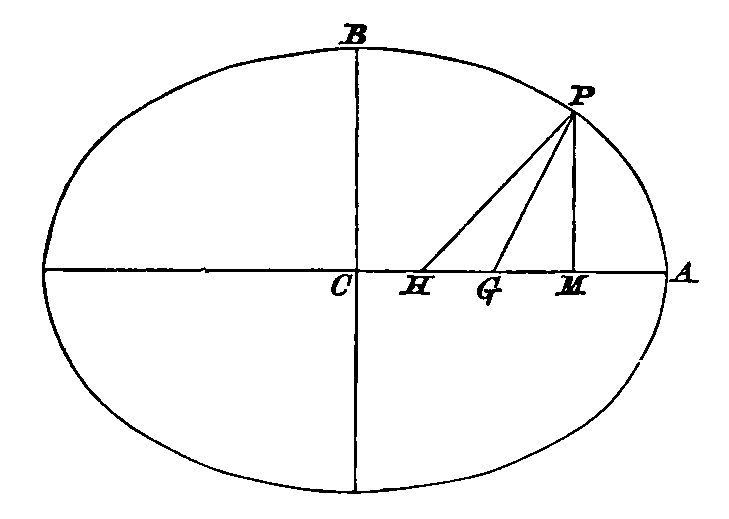
\includegraphics[width=0.6\textwidth]{114.png}
\centering
\end{figure}

Then Stirling says, when there is no rotation \(PH\) is the
direction of gravity and proportional to the value of it.

Draw \(PM\) perpendicular to \(CA\); let \(CM = x\), and \(PM = y\); let
\(X\) and \(Y\) denote the attractions at \(P\) parallel to \(CA\) and \(CB\)
respectively. Then if \(\rho\) denote the density, and \(e\) the excentricity,
we have by the modern theory
\[
X = 2\pi\rho (1 - e^2) x \int_0^{\tfrac{\pi}{2}} \sin^3 \theta (1 - e^2 \sin^2 \theta)^{-1} d\theta,
\]
%%-----File: 115.png-----%%
\[Y = 4 \pi \rho y \int_0^{\tfrac{\pi}{2}} \cos^2 \theta \sin \theta (1 - e^2 \sin^2 \theta)^{-1} d\theta;\]
see \textit{Statics}, Chapter \textsc{xiii}.

If we neglect \(e^4\) and higher powers of \(e\) we shall obtain
\[X =\frac{ 4 \pi \rho}{3} x \left(1 - \frac{e^2}{5}\right),\quad Y = \frac{4 \pi \rho }{ 3} y \left(1 + \frac{2 e^2}{ 5}\right);\]
thus
\[\frac{Y}{X} = \frac{y \left(1 + \dfrac{2 e^2}{5}\right)}{x\left(1 - \dfrac{e^2}{ 5}\right)} = \frac{ y}{ x \left(1 - \dfrac{3 e^2} { 5}\right)}\]
approximately.

But by the nature of the ellipse \(CG = e^2 x\), so that
\[CH = \frac{3 e^2 x}{5}\text{, and } HM = x \left(1 - \frac{3 e^2}{5}\right).\]

Thus the component attractions may be represented by \(PM\)
and \(MH\) in magnitude and direction; and therefore the resultant
may be represented by \(PH\) in magnitude and direction.

When there is rotation and relative equilibrium \(PG\) represents
the resultant action in magnitude and direction. Stirling does
not make any distinction in language corresponding to the fact
that this statement is \textit{exact} while the former is \textit{approximate}. We
know that for the equilibrium of a fluid, the resultant action must
be normal to the surface, so that \(PG\) is exactly the direction of
this action. Now take the expressions given for \(X\) and \(Y\), and
introduce the centrifugal force; then the actions at \(P\) parallel
to the axis of \(y\) and \(x\) respectively will be \(\mu y\) and \(\lambda x\), where \(\mu\)
and \(\lambda\) are constants: so that these actions are proportional to \(y\)
and \(\xp\dfrac{\lambda}{\mu} x\) respectively. But as we know that \(PG\) is the direction
of the resultant, the components must be proportional to \(PM\) and
\(MG\), respectively; hence \(MG\) must be equal to \(\xp\dfrac{\lambda }{\mu} x\), and \(PG\) will
represent the resultant in magnitude and direction.

This simple process does not occur very often in works on the
subject: it is given on page 113 of Laplace's \textit{Théorie \dots\ de la
Figure elliptique des Planetes}, at least substantially.
%%-----File: 116.png-----%%

\Section
154. Let \(\lambda\) denote the latitude of \(P\), that is, the angle \(PGM\):
this will of course be very nearly equal to the angle \(PCM\). We
can express \(PH\) and \(PG\) in terms of \(\lambda\) and the elements of the
ellipse; thus we obtain the following approximate results which
in effect Stirling gives: first suppose no rotation, then if \(F\) denote
the attraction at the pole, the attraction at \(P\) is \(F \xp\left(1 - \dfrac{e^2}{ 10} \cos^2 \lambda\right)\);
next suppose rotation, then if \(G\) denote the gravity at the pole,
the gravity at \(P\) is \(G \xp\left(1 - \dfrac{e^2}{2} \cos^2 \lambda\right)\).

In the diagram of Art.\ 153, the attraction at \(P\) is denoted by
\(PH\), and the gravity at \(P\) by \(PG\): thus, as Stirling remarks, \(HG\)
represents the centrifugal force at \(P\).

It is easy to give \textit{exact} statements of the nature of Stirling's
\textit{approximations}; this, as we shall see hereafter, was done by
Thomas Simpson.

\Section
155. Stirling applies the expression for the value of gravity
at any point of the surface to some observations respecting the
relative number of vibrations of the seconds pendulum at London
and at Jamaica; he deduces from these observations \(\xp\dfrac{1}{191}\) as the
ellipticity: but he goes on to shew that this value is inadmissible.

Stirling makes the following remark respecting pendulum
observations:

\begin{squote}
From all the Experiments made with Pendulums, it appears that the
Theory makes them longer in Islands, than they are found in fact\dots. This
Defect of Gravity in Islands is very probably occasioned by the Vicinity
of a great Quantity of Water, which being specifically lighter than Land,
attracts less in Proportion to its Bulk.
\end{squote}

Modern writers however appear to suggest that gravity may
be \textit{greater} on islands than on continents: see Airy's \textit{Figure of
the Earth} in the \textit{Encyclopædia Metropolitana}, page 230, and
Stokes's \textit{Variation of Gravity at the Surface of the Earth} in the
\textit{Cambridge Philosophical Transactions}, Vol.\ \textsc{viii}.

\Section
156. We have seen in Art.\ 44, that Newton assumed without
demonstration an oblatum as a possible form of relative equilibrium
for a mass of revolving fluid. Laplace asserts that the
%%-----File: 117.png-----%%
defect was first supplied by Clairaut in the \textit{Philosophical Transactions}
for 1737; see the \textit{Mécanique Céleste}, Vol.\ \textsc{v}.\ page 6. But
perhaps we may consider that Stirling had already obtained this
result. The main thing to be proved was that the resultant
action at any point of the surface would be normal to the surface,
when a proper relation was established between the ellipticity
and the ratio of the centrifugal force to the attraction. The relation,
in the notation we have used, is that \(\xp\dfrac{\lambda}{\mu} = \xp\dfrac{GM}{CM}\); that is,
\(\xp\dfrac{\lambda}{\mu} = 1 - e^2\). I do not say that Stirling gives this relation \textit{explicitly};
but it seems to me \textit{implied} in his remarks. Such too appears to
have been the opinion formed at the time; as we may infer from
a passage in the \textit{Philosophical Transactions}, Vol.\ \textsc{xl}.\ page 278,
which will be quoted in Art.\ 168. See also Lubbock, \textit{Account of
the Traité}\dots, page vi. However, Stirling's results were given without
demonstration; moreover, we find from the passage in the
\textit{Philosophical Transactions}, to which reference has just been made,
that they could not have been known to Clairaut when he wrote
his first paper on the subject; so that Clairaut's merits remain
undiminished.

\Section
157. I find it difficult to ascertain what opinion Stirling held
as to the agreement of the theory with facts. He says, as we
have seen, in his commencement referring to the Earth's elliptic
figure, ``that it is only nearly, and not accurately such.'' But
further on he says very positively:

\begin{squote}
And whereas the Earth could not be of an oblate spheroidical Figure,
unless it turned round its Axis; nor could it turn round its Axis,
without putting on that Figure\dots.
\end{squote}

Moreover he compares his theory with observation in the
case of Jupiter, and finds them to agree nicely; then he says:

\begin{squote}
And if this Theory agrees so well with Observations in \textit{Jupiter},
there is no doubt but it will be more exact in the Earth, whose Diameters
are much nearer to Equality.
\end{squote}

After he has made the suggestions respecting pendulum observations
on islands, which we have quoted, he gives the following
statements:

\begin{squote}
And I find by Computation, that the Odds in the Pendulums betwixt
%%-----File: 118.png-----%%
Theory and Practice is not greater than what may be accounted
for on that Supposition. I shall also observe, that although the Matter
of the Earth were entirely uniform, yet the Hypothesis of its being a
true Spheroid is not near enough the Truth to give the Number of Vibrations
which a Pendulum makes in twenty-four Hours.
\end{squote}

He concludes thus:

\begin{squote}
But after the \textit{French} Gentlemen who are now about measuring
a Degree, and making Experiments with Pendulums in the North and
South, shall have finished their Design, we may expect new Light in
this Matter.
\end{squote}

\Section
158. Stirling's mathematical powers were highly esteemed
by his contemporaries. Clairaut calls him ``one of the greatest
Geometricians I know in Europe.'' \textit{Philosophical Transactions},
Vol.\ \textsc{xl}.\ page 278. See also Maclaurin's \textit{Fluxions}, page 691;
Todhunter's \textit{History of the Theory of Probability}, pages 188, 190.

Stirling's name seems to be omitted in the ordinary biographical
dictionaries. The \textit{Abridgement of the Philosophical Transactions}
by Hutton, Shaw, and Pearson, contains some notices
entitled \textit{Biography; or, Account of Authors.} All that is there
recorded of Stirling is in Vol.\ \textsc{vi}.\ page 428, where we read: ``This
very respectable mathematician was agent for the Scotch Mine
Company, Leadhills. He died the 5th of December, 1770.'' Sir
John Leslie gives an interesting notice of Stirling in the \textit{Dissertation
on the Progress of Mathematical and Physical Science}, which
forms part of the \textit{Encyclopædia Britannica}: see page 711 in the
eighth edition of the \textit{Encyclopædia}.
%%-----File: 119.png-----%%
\Chapter{CHAPTER VI.}
\Subhead{CLAIRAUT.}
\Runhead{\textsc{clairaut.}}

\Section
159. \textsc{In} this Chapter we shall give an account of certain
memoirs by Clairaut; these exhibit the high mathematical power
of their author, and form the origin of the researches afterwards
embodied by him in his great work entitled \textit{Théorie de la Figure
de la Terre}.

\Section
160. In the Paris \textit{Mémoires} for 1733, published in 1735, we
have a memoir by Clairaut, entitled \textit{Détermination géométrique de
la Perpendiculaire à la Méridienne tracée par M. Cassini; avec
plusieurs Méthodes d'en tirer la grandeur et la figure de la Terre.}
The memoir occupies pages 406\dots 416 of the volume.

Clairaut shews that by such a process as Cassini adopted, the
curve of minimum length between its extreme points on the
surface of the Earth is obtained; and this curve is not in general
a plane curve, unless the Earth is a sphere.

Clairaut then proceeds to investigations respecting curves of
minimum length. For a surface of revolution he obtains the
property, now well known, that the sine of the angle made by the
curve at any point with the meridian varies inversely as the
length of the perpendicular from the point on the axis of revolution.
He gives special attention to the case in which the surface
is an ellipsoid of revolution.

A mistake occurs on page 414, which also influences page 416.
Clairaut says that if \(m\) is greater than unity \(u^2 - 1 + \xp\dfrac{u^2}{p^2}\) is obviously
%%-----File: 120.png-----%%
greater than \(\xp\dfrac{u^2-1} {m^2} + \xp\dfrac{u^2}{p^2}\); but \(u^2-1\) is a negative quantity, and so
his statement is wrong.

\Section
161. In the Paris \textit{Mémoires} for 1735, published in 1738, we
have a memoir by Clairaut entitled \textit{Sur la nouvelle Méthode de
M. Cassini, pour connoître la Figure de la Terre}. The memoir
occupies pages 117\dots 122 of the volume.

This memoir consists of simple and interesting investigations
of the geometrical theorems involved in the application of Cassini's
method.

An important proposition in solid geometry occurs here, perhaps
for the first time. At any point, \(M\), of a surface of revolution,
let a normal section be made at right angles to the plane
of the meridian; then the radius of curvature of this section at \(M\)
is the length of the normal between \(M\) and the axis of revolution.
Clairaut's demonstration is sound; but he leaves to his readers
the trouble of constructing a diagram without any directions.

\Section
162. In the Paris \textit{Mémoires} for 1736, published in 1739, we
have a memoir by Clairaut, entitled \textit{Sur la Mesure de la Terre par
plusieurs Arcs de Méridien pris à différentes Latitudes}. The
memoir occupies pages 111\dots 120 of the volume.

Let \(x\) be the abscissa and \(y\) the ordinate of any point on a
curve; and suppose that the radius of curvature is equal to
\(a + bA + cA^2 + \ldots\), where \(A\) is the angle whose tangent is \(\xp\dfrac{dx}{dy}\), and
\(a\), \(b\), \(c\), \dots\ are constants. Then Clairaut shews how we may express
\(x\) and \(y\) in terms of \(z\), which denotes the sine of \(A\).

He practically confines himself to the case in which the above
series contains only the three terms explicitly given; and for this
case he calculates some numerical results which might be useful
for application to the arcs about to be measured in Lapland and
Peru, compared with that measured in France.

Let \(m\) denote the excess of the radius of curvature at the
equator above that at latitude \(45°\), and let \(p\) denote the excess of
%%-----File: 121.png-----%%
the radius of curvature at latitude \(45^{\circ}\) above that at \(67^{\circ}\); then
Clairaut finds \({a - \xp\dfrac{2551m+2904p}{3283}}\) for the equatorial semi-diameter,
and \(a + \xp\dfrac{200m-2263p}{3283}\) for the polar semi-diameter. I have corrected
a sign in the former value. On the Cassinian hypothesis
\(m\) and \(p\) will both be positive, on the Newtonian hypothesis they
will both be negative.

\Section
163. We have next to consider a memoir by Clairaut entitled
\textit{Investigationes aliquot, ex quibus probetur Terræ figuram secundum
Leges attractionis in ratione inversâ quadrati distantiarum maximè
ad Ellipsin accedere debere, per Dn.\ Alexin Clairaut}, \textit{Reg.\ Societ.\
Lond.\ et Reg.\ Scient.\ Acad.\ Paris.\ Soc.}

This memoir occupies pages 19\dots 25 of Number 445 of the
\textit{Philosophical Transactions}; which is for the months January\dots\,June,
1737. The Number forms part of Vol.\ \textsc{xl.}\ which is for the
years 1737, 1738, and is dated 1741.

The object of the memoir is to demonstrate Newton's postulate;
see Art.\ 44. Clairaut obtains an approximate expression for the
attraction of an oblatum at any point of its surface; and thus
shews, that with a suitable value of the ellipticity the resultant of
the attraction and centrifugal force at any point of the surface
will be normal to the surface at that point.

\Section
164. In Clairaut's work on the \textit{Figure of the Earth} he did not
reproduce this approximate solution of the problem of the \textit{homogeneous}
oblatum; for Maclaurin had in the meantime given an
exact determination of the attraction of such a body, and so
Clairaut followed him and exhibited an exact solution: see
Clairaut's \textit{Figure de la Terre}, page 157. But the method used
in this memoir for the homogeneous oblatum is used in the
work for the heterogeneous oblatum: pages 233\dots 243 of the
work reproduce the essence of this very ingenious method.

\Section
165. In this memoir we have for the first time the approximate
method of determining the attraction of an oblatum on a
%%-----File: 122.png-----%%
particle at its pole, which still retains a place in elementary works:
see \textit{Statics}, Art.\ 217. The method occurs in the \textit{Figure de la
Terre}, pages 239\dots 243, where it is used for a particle situated at
any point of the polar axis produced.

\Section
166. We may observe that Clairaut's memoir begins rather
inauspiciously by apparently adopting the error we have noticed
in Newton and David Gregory: see Arts.\ 33 and 84. However, as
we proceed we find that Clairaut really understood the theorem
correctly: see especially page 24 of the memoir, and also pages
188\dots 190 of the \textit{Figure de la Terre}.

\Section
167. The next memoir is entitled, \textit{An Inquiry concerning the
Figure of such Planets as revolve about an Axis, supposing the
Density continually to vary, from the Centre towards the Surface;
by Mr.\ Alexis Clairaut}, F.R.S. \textit{and Member of the Royal Academy
of Sciences at Paris. Translated from the French by the Rev.
John Colson, Lucas.\ Prof.\ Math.\ Cantab.\ and F.R.S.}

This memoir occupies pages 277\dots 306 of Number 449 of the
\textit{Philosophical Transactions}, which is for the months August and
September, 1738. The Number forms part of Vol.\ \textsc{xl.}

\Section
168. Clairaut begins by adverting to Newton's researches on
the Figure of the Earth, and especially to his important postulate;
see Art.\ 44. Clairaut says:

\begin{squote}
What at first seem'd to me worth examining, when I apply'd myself
to this Subject, was to know why Sir \textit{Isaac} assumed the Conical
Ellipsis for the Figure of the Earth, when he was to determine its
Axis\dots.

I began then with convincing myself by Calculation, that the Meridian
of the Earth, and of the other Planets, is a Curve very nearly
approaching to an Ellipsis; so that no sensible Error could ensue by
supposing it really such. I had the Honour of communicating my
Demonstration of this to the \textsc{Royal Society}, at the Beginning of the
last Year; and I have since been inform'd, that Mr \textit{Stirling}, one of the
greatest Geometricians I know in \textit{Europe}, had inserted a Discourse in
the \textit{Philosophical Transactions}, No.\ 438.\ wherein he had found the same
thing before me, but without giving his Demonstration. When I sent
%%-----File: 123.png-----%%
that Paper to \textit{London}, I was in \textit{Lapland}, within the frigid \textit{Zone}, where
I could have no Recourse to Mr \textit{Stirling}'s Discourse, so that I could not
take any Notice of it.
\end{squote}

Of course Clairaut did not demonstrate, as he says, that the
meridian \textit{is} nearly an ellipse, but only that an ellipse is \textit{an} approximate
solution. As we have stated in Art.\ 130, the earlier
writers often \textit{assumed} that a fluid mass, if acted on by no external
force, would \textit{necessarily} assume a spherical form. In like manner,
when Newton's postulate had been established, it was often assumed,
as here implicitly by Clairaut, that a fluid mass rotating
with uniform angular velocity, and in relative equilibrium, would
\textit{necessarily} assume the form of an oblatum.

\Section
169. The first part of the present memoir determines the
attraction at any point of an ellipsoid of revolution, supposing it
to be composed of similar strata varying in density. The investigations
are only approximate, extending to the first power of
the ellipticity.

All that this part of the memoir contains is included in
Clairaut's \textit{Figure de la Terre}; but in the work there is a gain both
as to simplicity and to generality. Problem I. of the memoir corresponds
to Section 45 on pages 239\dots 243 of the work. Problem
II. and Problem III. of the memoir are included in Section
46 on pages 243\dots 247 of the work. The Theorem on page 282
of the memoir corresponds to Section 44 on pages 236\dots 239 of
the work. Problem IV. of the memoir corresponds to Sections
24 and 25 on pages 200\dots 202 of the work. Problem V. of the
memoir corresponds to Section 26 on pages 203\dots 208 of the
work; the investigation is given at full in the work, but only the
result in the memoir. Problem VI. and Problem VII. of the memoir
are included in Section 29 on pages 209\dots 218 of the work.

The work is more general than the memoir. In the memoir
it is assumed that the strata are similar, so that the ellipticity is
the same for all the strata; in the work this is not assumed. In
the work the formulæ contain a general symbol to represent the
density; in the memoir a law of density is assumed, the density
being denoted by \(fr^p + gr^q\), where \(f\), \(g\), \(p\), \(q\) are constants, and \(r\) is
%%-----File: 124.png-----%%
the variable polar semi-axis of the strata: the integrations are
effected in the memoir, but the formulæ are thus rendered less
simple in appearance than they are in the work.

\Section
170. The second part of the memoir contains the application
of the first part, to find the figure of a nearly spherical fluid mass
which rotates about an axis.

This part is unsatisfactory, because the only condition of equilibrium
which Clairaut regards is, that the resultant action at
every point of the free surface shall be normal to the surface at
the point. This is not \textit{sufficient} for the equilibrium of a heterogeneous
fluid mass. Clairaut discovered his error, and acknowledged
it; see page 155 of his \textit{Figure de la Terre}: here he allows
that his investigations in the memoir are untenable, except on the
supposition that the interior parts of the Earth had been originally
solid. In the Sections 37 and 39, on pages 225, 226, 228, and
229 of the work, we have an equivalent for pages 288\dots 294 of the
memoir, but expressed more accurately.

\Section
171. On page 294 of the memoir, we have the first appearance
of the theorem which is now known as \textit{Clairaut's Theorem}:
see Section 49, on pages 249, 250 of the \textit{Figure de la Terre}. We
will state the theorem. From the value of gravity at the pole
subtract the value of gravity at the equator, and divide the remainder
by the value of gravity at the equator; this fraction we
shall call \textit{Clairaut's fraction}. Then Clairaut's Theorem asserts
that \textit{the sum of the ellipticity of the surface and Clairaut's fraction
is equal to twice the ellipticity of the Earth considered as a homogeneous
fluid}. We shall defer the demonstration of the theorem
until we give an account of Clairaut's \textit{Figure de la Terre}.

\Section
172. Clairaut deduces from his theorem a result contrary to a
statement made by Newton; see Art.\ 30.

Clairaut, speaking of Newton, says:

\begin{squote}
He affirms, that the Earth is denser towards the Centre than at the
Superficies, and more depress'd than his Spheroid requires. But by the
foregoing Theory we may easily perceive, that if the Density of the
Earth diminishes from the Centre towards the Superficies, the Diminution
%%-----File: 125.png-----%%
of Gravity from the Pole towards the Equator will be greater than
according to Sir \textit{Isaac's} Table; but at the same time the Earth will not
be so much depress'd as his Spheroid requires, instead of being more so,
as he affirms.
\end{squote}

The two statements made by Clairaut are connected by his
Theorem, so that one will follow from the other. In the Section
38, on pages 226, 227 of his work, he shews that if the density diminishes
from the centre to the surface, the ellipticity is \textit{in general}
less than for the homogeneous body: the condition which prevents
the statement from being universally true is there given.

Clairaut proceeds to say:

\begin{squote}
Yet I would not by any means be understood to decide against Sir
\textit{Isaac}'s Determination, because I cannot be assured of his Meaning,
when he tells us, that the Density of the Earth diminishes from the
Centre towards the Circumference. He does not explain this, and
perhaps instead of the Earth's being compos'd of parallel Beds or \textit{Strata},
its Parts may be conceived to be otherwise arranged and disposed, so as
that the Proposition of Sir \textit{Isaac} shall be agreeable to the Truth.
\end{squote}

In his \textit{Figure de la Terre}, however, Clairaut does not hesitate
to decide against Newton: see Art.\ 30.

\Section
173. As an example, Clairaut takes the following case:

\begin{squote}
Setting aside all Attraction of the Parts of Matter, if the Action of
Gravity is directed towards a Centre, and is in the reciprocal Ratio of
the Squares of the Distances, the Ratio of the Axes of the Spheroid will
then be that of 576 to 577: And the Gravity at the Pole is greater
than at the Equator by \(\xp\dfrac{1}{144}\)th Part, or thereabouts. Which may be a
Confirmation of what is here advanced, especially to such as will not be
at the Pains of going through the foregoing Calculations. For we may
consider the Spheroid now mention'd, in which Gravity acts in a
reciprocal Ratio of the Squares of the Distances, as composed of Matter
of such Rarity, in respect of that at the Centre, that the Gravity is
produced only by the Attraction of the Centre or Nucleus.
\end{squote}

This is the first appearance of a problem which may be described
as a companion to that discussed by Huygens; and which
has sometimes been erroneously ascribed to Huygens: see Art.\ 64.
%%-----File: 126.png-----%%

\Section
174. Clairaut makes some remarks on the two principles which
were then in use for determining the form of a fluid in equilibrium,
namely, Newton's principle of balancing columns and
Huygens's principle of the plumb-line: he states the reasons which
induced him to adopt the latter principle. He proceeds to examine
whether the solution which he has obtained does make the
polar and equatorial columns balance; he finds that, in order to
secure this, a certain relation must hold among the constants
which enter into the expression for the density. In fact, as we
have already stated, Clairaut's solution in the memoir did not
satisfy all the necessary conditions: see Art.\ 170.

\Section
175. Clairaut demonstrates a result on pages 302\dots 304 of
the memoir, which though quite obvious on the modern theory
of fluid equilibrium must have appeared remarkable at the time.
We will state the general proposition of which his result is a
particular case. Suppose a solid, not necessarily homogeneous,
covered with a stratum of homogeneous fluid which is in equilibrium;
then if a fine channel be made in the body from one
point of the fluid to another, and be filled with the fluid, the
fluid in the channel will remain in equilibrium. In fact, the
pressure \(p\) at any point of the channel of fluid can theoretically
be found so as to satisfy the necessary conditions.

\Section
176. The memoir closes with some reference to the results
obtained by observations. Clairaut admits that those furnished
by the expedition to Lapland do not agree well with the theory;
for, according to these, each of the two fractions which occurs in
\textit{Clairaut's Theorem} is greater than \(\xp\dfrac{1}{230}\). However he will wait
for the observations made in Peru.

\Section
177. In the Paris \textit{Mémoires} for 1739, published in 1741,
there is a memoir by Clairaut, entitled \textit{Suite d'un Mémoire donné
en 1733, qui a pour titre: Détermination Géométrique de la Perpendiculaire
à la Méridienne, \&c.} The memoir occupies pages
83\dots 96 of the volume.

In modern language we should say that this memoir relates
to geodesic curves on the surface of an ellipsoid of revolution.
%%-----File: 127.png-----%%
The investigations are approximate, extending to the first power
of the ellipticity.

It may be interesting to give a specimen of Clairaut's investigations.

Let the polar semi-diameter be taken for unity, and let \(\xp\dfrac{1}{m}\)
denote the equatorial semi-diameter. Let \(x\) denote the longitude
of any point in a geodesic curve, measured from the meridian
which the geodesic curve crosses at right angles; let \(t\) denote
the cotangent of the latitude of this point; let \(p\) denote the
value of \(t\) when \(x=0\); then
\[
\frac{dx}{dt} = \frac{pm\xsurd(1+t^2)} {t\xsurd(t^2+m^2)\xsurd(t^2-p^2)}\text{.}
\]

Clairaut established this formula in his memoir of 1733; and it
may be easily obtained from well-known works on solid geometry.

Now put \(m=1-\alpha\), and suppose \(\alpha\) so small that its square
may be neglected; thus we get
\[
\frac{dx}{dt} = \frac{p} {t\xsurd(t^2-p^2)} - \frac{\alpha pt} {(1+t^2)\xsurd(t^2-p^2)} \text{:}
\]
hence
\[
x = \sin^{-1} \frac{\xsurd(t^2-p^2)} {t} - \frac{\alpha p} {\xsurd(1+p^2)} \sin^{-1} \frac{\xsurd(t^2-p^2)} {\xsurd(1+t^2)}. \tag{1}
\]

Clairaut does not use the symbol \(\sin^{-1}\); but he proposes the
symbol \(As\) to denote what we denote by \(\sin^{-1}s\).

The equation (1) determines \(x\) when \(t\) is known. Now
Clairaut proceeds to determine \(t\) from it when \(x\) is known; and
for this he employs a special process, which we will now explain.

Suppose that \(t=\tau+\Delta\tau\), where \(\tau\) is the value of \(t\) which
would correspond to the known value of \(x\) when \(\alpha\) is zero, and so
\(\Delta\tau\) is very small. Hence from (1) we get
\begin{multline}
x = \sin^{-1} \frac{\xsurd(\tau^2-p^2)}{\tau} + \frac{p}{\tau\xsurd(\tau^2-p^2)} \Delta\tau - \frac{\alpha p}{\xsurd(1+p^2)} \sin^{-1} \frac{\xsurd(\tau^2-p^2)}{\xsurd(1+\tau^2)}\\
- \frac{\alpha p\tau\Delta\tau}{(1+\tau^2)\xsurd(\tau^2-p^2)}. \tag{2}
\end{multline}
%%-----File: 128.png-----%%
But by supposition \(x = \sin^{-1} \xp\dfrac{\sqrt{(\tau^2 - p^2)}}{\tau}\).

Hence, neglecting the term which involves the product of
\(\alpha\) and \(\Delta\tau\), we have from (2)
\[\frac{p}{\tau\xsurd{(\tau^2 - p^2)}} \Delta\tau = \frac{\alpha p}{\xsurd(1 + p^2)} \sin^{-1}\frac{ \xsurd(\tau^2 - p^2) }{ \xsurd(1 + \tau^2)}.\]

This furnishes the correction \(\Delta\tau\), which will be required in the
cotangent of the latitude when calculated for a sphere, in order
to obtain the value for the ellipsoid of revolution.

Clairaut himself uses \(t\) for our \(\tau\), and \(dt\) for our \(\Delta\tau\).

Clairaut's memoir consists of the solution of four problems;
the other three resemble that which we have taken as a specimen.
They are illustrated by numerical application to an oblatum in
which \(\alpha = \xp\dfrac{1}{100}\); this value Clairaut says does not differ much
from that obtained by means of the degree of the meridian measured
at the polar circle.

This memoir is the last of the series of Clairaut's contributions
to our subject before the publication of his work entitled \textit{Théorie
de la Figure de la Terre}, which we shall examine in Chapter XI.:
we now proceed to give an account of the measurement in Lapland,
to which allusion has just been made.
%%-----File: 129.png-----%%
\Chapter{CHAPTER VII.}
\Subhead{ARC OF THE MERIDIAN MEASURED IN LAPLAND.}
\Runhead{\textsc{arc of the meridian measured in lapland.}}

\Section
178. \textsc{The} Academy of Sciences at Paris seems to have selected
the problem of the Figure of the Earth as peculiarly its own.
But the success hitherto attained scarcely corresponded to the
labour which had been expended; partly perhaps owing to the
fact that the able observers, trained by the astronomers who bore
the justly celebrated name of Cassini, had adopted the oblong
form and maintained it firmly.

In order to settle the question in dispute between the Cassinians
and the Newtonians, the scheme was seriously proposed in 1733 of
measuring an arc of the meridian near the equator, in order to
compare the corresponding length of a degree with that which had
been obtained from the French arc by Picard and by J. Cassini.
The task was entrusted to three members of the Academy,
Bouguer, La Condamine, and Godin, who started in May, 1735.
Two Spanish naval officers, Juan and Ulloa, assisted in the work.

\Section
179. After this expedition had started for Peru it was resolved
to measure also an arc as near as possible to the pole: see
La Condamine, \textit{Journal du Voyage} \dots\ page 1. This task was
entrusted to four members of the Academy, Maupertuis, Clairaut,
Camus, and Le Monnier; moreover l'Abbé Outhier, who was a
correspondent of the Academy, and Celsius, who was professor of
Astronomy at Upsal, were associated with the Academicians.

\Section
180. The Arctic expedition seems to me to have been stronger
than the Equatorial. The genius of Clairaut outshone that of the
%%-----File: 130.png-----%%
whole Academy, which was not yet adorned by the rising splendour
of D'Alembert. But even if we leave out of consideration
this transcendant name the superiority remains, I think, still
with the Arctic party. I should place Maupertuis, Camus, and
Le Monnier, above Bouguer, La Condamine, and Godin; while
the priest and the professor who accompanied the former are
at least equal to the two sailors who assisted the latter.

The two operations were conducted on different principles.
The members of the Arctic expedition worked in harmony under
the general direction of Maupertuis. La Condamine calls
Maupertuis, the senior (\textit{l'ancien}) of the party, \textit{Journal du Voyage} \dots\
page iii.; and Maupertuis is called \textit{Chef de l'entreprise du Nord}
in the \textit{Histoire de l'Académie} \dots\ for 1737, page 96. There was but
little cordiality in the Equatorial party; and the three Academicians
performed much of their work separately. Thus in the
former case we find friendship and subordination; and in the
latter case isolation and independence. On a purely scientific
estimate it may be maintained that there are advantages in each
course which the other does not secure.

We are here concerned only with the Arctic party which left
Paris on the 20th of April, 1736. Two narratives of the proceedings
were printed; we will now describe these works.

\Section
181. Maupertuis published \textit{La Figure de la Terre déterminée
par les observations \dots\ au cercle polaire}. Paris, 1738. This is an
octavo volume; the Title, Preface, and Table of Contents, occupy
xxviii.\ pages; the text occupies 184 pages; there are 9 plates
besides a map.

In the historical portion of the Paris \textit{Mémoires} for 1737, pages
90\dots 96 relate to the Arctic expedition: the date of publication is
1740. Moreover, in this volume, pages 1\dots 130 of Maupertuis's
work are reprinted; they occupy pages 389\dots 465 of the volume.
Maupertuis here says there have been too many editions of his
book in various languages to render it necessary to repeat the
other observations made in the North: he contents himself with
referring to the observations on the force of gravity, and reproduces
the Table which occurs on page 181 of his book.
%%-----File: 131.png-----%%

It is stated by La Condamine that Maupertuis's work was
translated into all the languages of Europe: \textit{Journal du Voyage} \dots\
page iii. I have seen a German translation and a Latin translation.
The German translation was published at Zurich in 1741;
it contains also a dedication to Frederic III. of Prussia, by Samuel
König, an introduction by the translator, and a memoir by Celsius
on Cassini's work \textit{De la Grandeur et de la Figure de la Terre}. The
Latin translation was published at Leipsic in 1742; it contains
also an introduction by the translator, Alaricus Zeller: he says
on the third page of his introduction that he has preserved the
paging of the Amsterdam edition in his margin. This translator's
introduction contains some criticisms which are not devoid of
interest; they do not however practically affect the determination
of the length of the degree of the meridian, but relate to incidental
matters, such as refraction. There are also a few notes to
the translation, which supply corrections of slight misprints or
mistakes.

There is an English translation which I have not seen.

\Section
182. Outhier published \textit{Journal d'un Voyage au Nord}\dots, Paris,
1744. This is a quarto volume; the Half-title, Title, Dedication,
and Preface, are on eight pages; the text occupies 238 pages,
followed by two pages which contain an \textit{Extrait des Registres de
l'Académie}\dots, and the \textit{Privilege du Roi}. According to the \textit{Table
des Figures} on page 238, there ought to be 18 plates. But in the
single copy which I have seen there are only 16 plates. The plate
which is marked 15 in the list does not occur; there is only one
plate corresponding to the two which are marked 9, 10 on the
list; and there are only two plates corresponding to the three
which are marked 6, 7, 8 on the list. On the other hand, there is
a \textit{Veüe de la Montagne de Niemi, du côté du Midy}, which is not
named in the list.

Outhier's work seems never to have attracted much attention
and to be now scarce.

\Section
183. The calculations and the theoretical deductions are given
most fully by Maupertuis; the details of the daily occupations of
the party, and the peculiarities of the country and of the inhabitants,
%%-----File: 132.png-----%%
are given most fully by Outhier. I shall refer to the pages
of Maupertuis in the original French edition, and distinguish them
by the letter M. I shall refer to Outhier's work by the letter O.

\Section
184. Maupertuis was for a long time in doubt whether he
should go to Iceland, to Norway, or to the Gulf of Bothnia; he
decided for the last, intending to carry on his operations among
the islands along the shores of the Gulf. O. 3. But on examination
these islands were found to be too low, and too near the shore,
to form advantageous stations; and after some consideration
Maupertuis resolved to proceed to the mountains north of Tornea,
which is at the head of the Gulf. M. 11; O. 52.

Finally Tornea was taken as the most Southern station, and
Kittis as the most Northern; both are on the river Tornea, and
nearly on the same meridian. The other stations were mountains
not far from the river. The base which was to be measured was
chosen about midway between Tornea and Kittis, and the extremities
denoted by signals. M. 29; O. 86.

All the geodetical angles were observed in the space of about
two months, between the beginning of July and the beginning of
September, 1736. The observations were made with a quadrant
of two feet radius. M. 33, 79; O. 204\dots 219.

\Section
185. The next step was to determine the difference of latitude
of the extreme points of the arc. The star \(\delta\) Draconis was selected
which passed the meridian very near to the zenith; observations
of this star were made at Kittis on the 4th, 5th, 6th, 8th, and 10th
of October; and at Tornea on the first five days of November.
The difference of zenith-distance was found to be \(57'\ 25''.\,55\).
M. 104.

The instrument used for determining this difference of zenith-distance
was a zenith-sector made by Graham at London; the
instrument resembled that used by Bradley in the observations
which established the aberration of light. M. 38. A copper
telescope-tube of nine feet long formed one radius of the sector;
the extent of the arc of the sector was \(5°\frac{1}{2}\), graduated at every \(7'\frac{1}{2}\).
At the focus of the telescope were fixed two wires at right angles.
%%-----File: 133.png-----%%
The telescope and the arc formed one instrument. A large
pyramid of wood 12 feet high served as the support of the instrument.
M. 38, 94. The instrument could turn freely round a horizontal
axis; it was moved by a micrometer screw acting in opposition
to a weight. A plumb-line was suspended from the centre
of motion, and marked on the graduated arc the angle through
which the instrument had been turned. The absolute zenith-distance
of a star at a given place was not determined by the
French observers, but only the \textit{difference} of zenith-distance at
two given places.

\Section
186. The base was measured on the frozen surface of the river
Tornea, very nearly in the direction of the stream; the extremities
of the base were on the land. The measurement was begun on
December 21st, and occupied a week. Eight rods of fir were
employed, each five toises long; the correct length of these rods
was determined by the aid of an iron toise which had been carefully
adjusted to the length of the standard toise at Paris. O. 137.
This iron toise is known henceforth in the history of the subject as
the \textit{Toise du Nord}. A similar iron toise had been taken by the
Equatorial expedition, which is known as the \textit{Toise du Pérou}.
Neither Maupertuis nor Outhier records the fact that these two
toises were made at the same time and by the same artist,
Langlois; this we learn from La Condamine: see the Paris
\textit{Mémoires} for 1772, Part \textsc{ii}.\ pages 482\dots 501.

\Section
187. The measurers of the base divided themselves into two
bands; each band had four of the fir rods, and measured independently:
the length of the base was found to be 7406 toises 5 feet
4 inches by one band, and 7406 toises 5 feet by the other band.
After the measurement was finished three of the party verified
that no error could have arisen in counting the hundreds, by using
a cord 50 toises long over the whole base. O. 144.

The sun scarcely rose above the horizon, but the twilight, the
white snow, and the Aurora Borealis supplied enough light for
four or five hours work daily. M. 51.

\Section
188. It followed from the length of the base that the length
of the arc of the meridian intercepted between the parallels of
%%-----File: 134.png-----%%
Tornea and Kittis was \(55023\frac{1}{2}\) toises; and that the length of a
degree of the meridian at the Arctic circle was nearly \(1000\) toises
greater than the length calculated according to the Cassinian theory
in the book \textit{De la Grandeur et de la Figure de la Terre}. M. 58.

The party then went to Tornea and remained shut up in their
chambers in a kind of inaction until March. The difference
between their result and that of the Cassinian theory was so great
that it astonished them; and although they considered their
operations to be incontestable, yet they resolved to execute some
rigorous verifications. M. 63. We read in the Paris \textit{Mémoires} for
1737, page 94 of the historical portion:

\begin{squote}
On la tint fort secrette, tant pour se donner le loisir de la réflexion
sur une chose peu attendue, que pour avoir le plaisir d'en apporter à
Paris la premiére nouvelle.
\end{squote}

\Section
189. The angles of the triangles were supposed to admit of
no doubt; these angles had been observed many times by various
persons; and the three angles of every triangle had been observed.
The calculations were verified by combining the triangles in a
different series; and also by assuming that errors had arisen in
measuring the angles, which all tended to make the length greater
than it should have been. But the length of the arc of the
meridian still remained without any very decided diminution.
M. 63\dots 65.

The measurement of the base was considered to be also above
suspicion; thus there remained only the very important point of
the difference in latitude of the extreme stations; and accordingly
this was redetermined. The star \(\alpha\) Draconis was now selected;
observations of this star on the meridian were made with the
zenith-sector at Tornea on the 17th, 18th, and 19th of March,
1737, and at Kittis on the 4th, 5th, and 6th of April: the difference
of zenith-distance was found to be \(57'\ 25''.\,85\). M. 115.

The reason given in the Paris \textit{Mémoires} for 1737, on page 95
of the historical portion, for going over the astronomical part of
the work again is that it could be done much more easily than the
other parts.

\Section
190. The observations for determining the difference of latitude
required corrections for aberration, for precession, and for
%%-----File: 135.png-----%%
a third inequality which had been recently discovered by Bradley,
and which is called nutation. No correction was applied for
refraction. M. 125. See Bouguer's \textit{Figure de la Terre}, page 290.

Thus, finally, the amplitude of the arc of the meridian was
\(57'\ 26''.\,93\) by the star \(\delta\) Draconis, and \(57'\ 30''.\,42\) by the star
\(\alpha\) Draconis; the difference is \(3''.\,49\). Maupertuis considered that
\(0''.\,95\) of this difference was owing to an inequality in the graduation
of the sector, which was discovered by careful scrutiny.
M. 124.

Maupertuis took the mean of the two results, \(57'\ 28''.\,67\) for
the amplitude; and from this he deduced that the length of the
degree of the meridian which is bisected by the Arctic circle is
57437.9 toises.

\Section
191. Important pendulum experiments were made at Pello,
which is close to Kittis. The result is that a pendulum which
oscillates in a second at Paris will make 59 more oscillations in
24 hours at Pello than at Paris. M. 172.

\Section
192. The Academicians endured great hardships during their
operations. The severe cold of the winter months must have been
anticipated; and the precautions which the natives had learned
from experience would afford some mitigation of this evil. But
the most painful period of the survey seems to have been that
which was spent among the mountains in observing the geodetical
angles: in one instance they remained for ten days on a mountain.
M. 21. The exposure to extremes of heat and of cold, the excessive
rains, and the want of proper food, all contributed to the
sufferings of the party. But the worst torment seems to have
been that inflicted by insects. Maupertuis calls them flies, and
says they were of different kinds. M. 14, 16, 22. Outhier calls
them by various names; flies, gnats, midges: thus \textit{cousins} 55, 57,
58, 59, 63, 64, 74, 82; \textit{moucherons} 64, 65, 75, 79, 82; \textit{mouches}
57, 58, 64. Le Monnier fell very ill. M. 24; O. 75, 79, 81. According
to Hutton's \textit{Mathematical Dictionary} the health of Maupertuis
was permanently impaired by the hardships he underwent.

The Academicians left Tornea in June, 1737, and reached Paris
in August.
%%-----File: 136.png-----%%

\Section
193. The measurement of the arc of the meridian by the
French in Lapland is historically the most important of all such
operations. The question as to the oblate or oblong form of the
Earth was decisively settled.

Two generations of the best astronomical observers formed in
the school of the Cassinis had struggled in vain against the
authority and the reasoning of Newton.

\Section
194. Some incidental matters may now be noticed which
present themselves in studying the narratives.

Maupertuis says on his page xii.:

\begin{squote}
Sur des routes de 100 degrés en Longitude, on commettroit des
erreurs de plus de 2 degrés, si naviguant sur le Sphéroïde de M. Newton,
on se croyoit sur celui du Livre de la Grandeur et Figure de la Terre.
\end{squote}

I cannot understand this. Nothing is said about the \textit{latitude};
but the amount of error in a course of 100 degrees of longitude
will depend mainly on the latitude.

In the life of Maupertuis in the \textit{Biographie Universelle}, which
is partly by Delambre, reference is made to the exaggerations of
Maupertuis on this point.

Clairaut is the mode of spelling which the bearer of this distinguished
name himself adopted: Outhier, however, generally
uses Clairaux; once he has Clairault. O. 25.

Maupertuis, in returning to France, was shipwrecked in the
Gulf of Bothnia; he merely alludes to this misfortune himself:
but we find from Outhier that the instruments were immersed,
and were cleaned rather more than a month after the accident.
M. 78; O. 169, 189.

\Section
195. The success of the Arctic expedition may be fairly
ascribed in great measure to the skill and energy of Maupertuis:
and his fame was widely celebrated. The engravings of the period
represent him in the costume of a Lapland Hercules, having a
fur cap over his eyes; with one hand he holds a club, and with
the other he compresses a terrestrial globe. Voltaire, then his friend,
congratulated him warmly for having ``aplati les pôles et les
Cassini.'' See articles entitled \textit{Histoire des Sciences} in the \textit{Revue
%%-----File: 137.png-----%%
des deux Mondes}, Jan.\ and Nov., 1869. Readers of Carlyle's
\textit{History of Frederick the Great} will remember the allusions to
the Earth-flattener.

\Section
196. Although the measurement of the Lapland arc settled
the question as to the oblate or oblong form of the Earth, yet it
introduced a great difficulty; for by comparing the result with
that obtained from the French arc the ellipticity of the Earth
appeared to be about \(\xp\dfrac{1}{178}\). This was greater than had been expected,
and greater than subsequent operations, such as that in
Peru, furnished. From our present knowledge it is certain that
this value of the ellipticity is far too large.

We have seen indeed, in Art.\ 177, that Clairaut assigned \(\xp\dfrac{1}{100}\)
as the ellipticity furnished by the Lapland arc; this must have
been obtained by using for the French arc a certain value obtained
by Maupertuis in his \textit{Figure de la Terre}, page 126; but this value
of the French arc was soon afterwards found to be too small.

\Section
197. According to La Lande, Maupertuis himself was not
satisfied with his operations. We read in the \textit{Bibliographie
Astronomique}:

\begin{squote}
\dots\ je sais que Maupertuis n'en était pas lui-même très-content.
Page 407.

\dots\ Au reste, on m'écrit de Suède que Maupertuis s'était proposé de
recommencer la mesure à ses dépens; ce qui prouve qu'il n'en était pas
très-content. Page 811.
\end{squote}

It is well known that the Lapland arc was remeasured at the
beginning of the present century by Svanberg and others under
the direction of the Stockholm Academy of Sciences. La Lande
alludes to the early stages of this operation; see the \textit{Bibliographie
Astronomique}, pages 811, 837, 857. Svanberg obtained a decidedly
shorter length for a degree of the meridian than that of
Maupertuis, namely, 57196.159 toises instead of 57437.9 toises;
but the middle points of the two degrees are not quite identical.

\Section
198. We may just notice the memoir by Celsius, which is
contained in the German translation of Maupertuis's \textit{Figure de la
%%-----File: 138.png-----%%
Terre}: see Art.\ 181. This is probably a translation of one which
was originally published at Upsal in 1738 under the title of \textit{De
observationibus pro figurâ telluris determinandâ in Galliâ habitis
disquisitio}, according to La Lande's \textit{Bibliographie Astronomique},
page 406.

In the translation Celsius first defends the astronomical operations
in Lapland from an objection which had been urged against
them by J. Cassini before the Paris Academy, because the sector
had not been reversed at each place of observation. Celsius maintains
that this was unnecessary for the purpose of the observers,
especially considering the excellence of Graham's sector. Then
Celsius proceeds to criticise the French operations recorded in the
work \textit{De la Grandeur et de la Figure de la Terre}; and he considers
that he shews both the astronomical and geodetical parts to be
untrustworthy. These operations indeed were just about to be
given up and replaced by the more accurate determinations recorded
in the work \textit{La Meridienne de Paris verifiée}.

\Section
199. For further information respecting the Lapland arc of
the meridian, I may refer to my memoir on the subject published
in the \textit{Cambridge Philosophical Transactions}, Vol.\ \textsc{xii}.; I have
there corrected the numerous and serious errors which have been
made by distinguished astronomers in their account of this remarkable
measurement.
%%-----File: 139.png-----%%
\Chapter{CHAPTER VIII.}
\Subhead{MISCELLANEOUS INVESTIGATIONS BETWEEN THE
YEARS 1721 AND 1740.}
\Runhead{\textsc{miscellaneous investigations from 1721 to 1740.}}

\Section
200. \textsc{We} have first to consider a production to which allusion
has been made in Arts.\ 143 and 150. It is entitled \textit{A Dissertation
concerning the Figure of the Earth, by the Reverend John
Theophilus Desaguliers,} L.L.D. F.R.S. This is contained in
Vol.\ \textsc{xxxiii}.\ of the \textit{Philosophical Transactions}: the volume is
for 1724, 1725; and is dated 1726.

The dissertation consists of four parts.

\Section
201. The first part occupies pages 201\dots 222 of the volume.
This part criticises the conclusions at which J. Cassini had arrived
as to the form of the Earth in his \textit{De la Grandeur et de la Figure
de la Terre}, of which we have given an account in Arts.\ 100\dots 108.

Desaguliers endeavours to shew that the Cassinian figure is
impossible, because it would lead to a deviation of the plumb-line,
from the direction which is at right angles to the surface of water,
to the amount of five minutes: but the process is unsound. We
know now that under certain hypotheses as to the form of
the solid nucleus, the outer surface of the fluid might be an oblongum:
see Clairaut's \textit{Figure de la Terre}, page 224.

Desaguliers maintains that the latitudes in the French survey
of the meridian cannot be relied on as sufficiently accurate to
establish the oblong figure of the Earth; and he is not satisfied
that the heights of the mountains were properly determined.
Desagulier's criticisms have perhaps some foundation; but like
many controversialists he seems disposed to be unfair. For instance,
%%-----File: 140.png-----%%
he considers that the height of one mountain was over-estimated,
and the height of another under-estimated; and thus,
he says, we must add 20 toises to the length of the 44th degree
of latitude, and take away 30 toises from the length of the 45th
degree of latitude. But even admitting these corrections to be
necessary, they tend to balance each other; and they produce
no perceptible effect on the definite result obtained by Cassini,
namely, that the whole southern arc from Paris to the Pyrenees
gives a longer average length of a degree than the whole northern
arc from Paris to Dunkirk.

Strictly speaking, what Desaguliers calls the 44th degree of
latitude should be the 45th; and what he calls the 45th should
be the 46th.

Desaguliers assigns one reason which may have induced Cassini
to make the Earth oblong, in these words: ``especially because
in this Hypothesis, the Degrees differ most in Length from
one another about the 45th Degree.'' But this is quite unsatisfactory.
For if we suppose the Earth to be nearly spherical, then
whether it be oblate or oblong the degrees will differ most in
length at about the 45th degree: see Art.\ 140.

\Section
202. The second part of the dissertation occupies pages
239\dots 255 of the volume. The object of this part is to shew
``How the Figure of the Earth is deduc'd from the Laws of
Gravity and Centrifugal Force.'' Instead of giving anything of
his own, Desaguliers transcribes a long extract from Keill's book
against Burnet; the extract consists of that matter which Keill
took substantially from Huygens: see Art.\ 74.

Desaguliers says:

\begin{squote}
I own indeed that he has made a Mistake in that Book concerning
the Measure of the Degrees of an Ellipse; but I find that all that
relates to the oblate Spheroidical Figure of the Earth is right\dots.
\end{squote}

The mistake of course is that which we have noticed in
Art.\ 76. Desaguliers would probably have thought it unnecessary
to warrant the accuracy of the matter which he transcribed, if he
had known that it was substantially all due to Huygens.
%%-----File: 141.png-----%%

\Section
203. The third part of the dissertation occupies pages
277\dots 304 of the volume. This part is chiefly a criticism of the memoir
by Mairan which we have examined in Arts.\ 109\dots 114. Much
of what Desaguliers says, though quite true, would have failed to
produce any effect on Mairan. For instance, according to Mairan,
Paris is more distant from the centre of the Earth than a place at
the equator is; \textit{hence the attraction at Paris will be less than} it is
at the equator; hence, although the centrifugal force at the equator
is greater than at Paris, we may have gravity at Paris less than
gravity at the equator: and this is contrary to observation. But
Mairan would have declined to admit the statement in Italics;
he had invented a law of attraction for himself which made the
attraction greater at Paris than at the equator.

Of course the assailable part of Mairan's memoir was the
arbitrary law of attraction which he had invented; and against
this Desaguliers directs a decisive argument. He finds that, taking
Mairan's law, and allowing for centrifugal force, the Paris seconds
pendulum would have to be shortened at the equator nearly an
inch. He says: ``But this being about five Times more than
agrees with Observation; what proves too much, proves nothing
at all.'' See Art.\ 52.

Desaguliers finds, that on Mairan's law the polar and equatorial
columns of fluid would not balance; but Mairan might
have replied that the Earth was solid, and for this reason he
might have declined to admit the principle of balancing columns.

\Section
204. Desaguliers in the third part of his dissertation returns
to the subject of the French arc. He arranges a table which
gives the observed latitudes of successive stations on the meridian,
and also the distance from Paris in toises. He shews that
there is not a constant decrease in the length of a degree in
passing from the southern extremity of the arc to the northern.
But the objection is of no value; because the French observers
did not require, and did not attempt to find, the latitudes of
intermediate stations with the same accuracy as the latitudes of
Paris and of the two extremities of the arc.

Desaguliers says on page 303:
%%-----File: 142.png-----%%

\begin{squote}
To conclude, I will propose a Method of observing the Figure of the
Shadow of the Earth in Lunar Eclipses, whereby the Difference between
the Diameters in the oblong spheroidical Figure, if there be such
an one as Mons.\ \textit{Cassini} affirms (\textit{viz}.\ of 96 to 95), may be discover'd.
\end{squote}

But the method has, I believe, no practical value.

\Section
205. The fourth part of the dissertation occupies pages
344, 345 of the volume. It consists of an account of an experiment
to ``illustrate'' what had been said in the preceding parts. The
essence of the experiment may be thus described. Take a hoop
of thin elastic steel; let it revolve round a diameter as axis, the
axis passing freely through the steel: then the greater the angular
velocity the more will the hoop bulge out into an oblate
form. The toy with which Desaguliers amused himself of course
proved nothing to the point; however, he boldly asserts that
from this experiment, compared with what had been said, ``it
will appear that the Earth cannot preserve its Figure, unless it
be an oblate Spheroid.''

\Section
206. There are some incidental matters of interest in the
dissertation which may be noticed.

Desaguliers suggests on page 209, that

\begin{squote}
\dots\ a Degree of Latitude shou'd be measur'd at the Æquator, and
a Degree of Longitude likewise measur'd there; and a Degree very
northerly, as for Example, a whole Degree might be actually measur'd
upon the \textit{Baltick} Sea, when frozen, in the Latitude of sixty Degrees.
\end{squote}

We read on pages 219, 220:

\begin{squote}
\dots\ when once an Hypothesis is set on Foot, we are too apt to
draw in Circumstances to confirm it; tho', perhaps, when examin'd impartially,
they may rather weaken, than strengthen our Hypothesis;
otherwise, the Author of the History of the \textit{Royal Academy}, for the
Year 1713, wou'd not have alledg'd, that \textit{the late Mons}.\ Cassini \textit{observ'd}
Jupiter \textit{to be oval}, as a Proof of young Mons.\ \textit{Cassini's} Hypothesis; because
\textit{Jupiter} is oval the other Way, that is, an oblate Spheroid flatted
at the Poles\dots.
\end{squote}

But I cannot find anything in the volume which justifies
this remark by Desaguliers.
%%-----File: 143.png-----%%

The only reference to Jupiter occurs after a notice of the
fact that the Earth deviates but little from a sphere; then we
read:

\begin{squote}
Si Jupiter est ovale, comme il l'a paru quelquefois à feu M.\ Cassini,
il faut qu'il le soit bien davantage pour le parôitre de si loin.
\end{squote}

It is obvious that these words do not bear any such meaning
as Desaguliers suggests.

Desaguliers refers to the opinion of Dr Burnet, which we have
noticed in Art.\ 74. Desaguliers says on his page 221: ``But Dr.\
\textit{Burnet}, afterwards, alter'd his Opinion, as I am credibly inform'd.''

Desaguliers asserts ``That a fluid Substance, of any Figure,
will by the Gravity of its Parts become spherical,\dots'' He gives
what he calls a demonstration of this on his pages 278, 279;
but, as might be expected, his demonstration is quite inconclusive.
See Art.\ 130.

Desaguliers adopts on his page 280 the erroneous notion that
by increasing the density of the central part of the Earth, the
ellipticity is also increased; see Arts.\ 30, 84 and 172. Newton
and David Gregory do not state whether they suppose the central
part still to remain fluid or to become solid. Desaguliers, however,
says distinctly, ``Then if, when the Central Parts are fix'd,
and the superficial \textit{Strata} are still fluid,\dots''

To shew that Desaguliers is wrong, we have only to put \(\alpha = 0\)
on page 219 of Clairaut's \textit{Figure de la Terre}; then we find that
\(\delta\) is less than \(\xp\dfrac{5 \phi }{4}\). Or see Simpson's \textit{Mathematical Dissertations},
page 30.

A paragraph which occurs on pages 280 and 281 is to be
cancelled, according to an Advertisement by Desaguliers at the
end of Number 399 of the \textit{Philosophical Transactions}.

\Section
207. Desaguliers, on his page 285, deviates from accuracy in
saying that ``on different Parts of the Surface of the Earth (in
the Condition it is now) the Gravity on Bodies is reciprocally as
their Distance from the Centre of the Earth.'' I have already
stated that this proposition should be enunciated thus: Gravity
%%-----File: 144.png-----%%
\textit{resolved along the radius-vector} varies inversely as the radius; see
Art.\ 33. Desaguliers omits the resolution along the radius-vector.
Moreover, I think from his context, and from a calculation on his
page 287, that he made another mistake, and supposed that the
\textit{attraction} along the radius-vector varied inversely as the radius;
that is, I think, he neglected the distinction between \textit{attraction}
and \textit{gravity}. On his pages 286 and 287 he assumes that for an
oblongum the gravity will vary inversely as the radius-vector;
and by gravity he means here \textit{attraction} alone, for he proceeds to
allow separately for the centrifugal force. The assumption is
unjustifiable, and seems to have arisen from the confusion of
gravity with attraction in the case of the oblatum.

\Section
208. Desaguliers obtained from a friend a ``Philosophical
Argument'' against Mairan; it is thus stated on his page 298:

\begin{squote}
If the Earth was of an oblong spheroidical Figure, higher at the
Poles than the Æquator; the Axis of its Revolution, wou'd either go
thro' one of its short Diameters, or be continually changing unless the
said Axis did exactly coincide with the Axis of the Figure.
\end{squote}

These words themselves are true; they are, however, applicable
to the oblatum if we change \textit{short} into \textit{long}. The so-called
\textit{demonstration} which follows shews that Desaguliers and his friend
were wrong in their notions on the subject. In modern language
these notions amount to considering that the rotation of an
oblongum round its axis of figure is \textit{unstable}. The mechanical
knowledge of the period was inadequate to the discussion of a
difficult problem in Rigid Dynamics.

\Section
209. A work was published at Padua in 1728, entitled
\textit{Joannis Poleni \dots\ Epistolarum Mathematicarum Fasciculus.} The
work is in quarto; the pages are not numbered.

One of the letters relates to the Figure of the Earth; it is
addressed ``Viro celeberrimo Abbati Gui.\ Grando.'' This letter
occupies eleven pages; it is of little importance.

Since some persons maintained that the Earth was oblate, and
others that it was oblong, Poleni considers it safer to adopt the
spherical form as a compromise between the two extremes. He
%%-----File: 145.png-----%%
suggests, however, that by measuring an arc of longitude, say in
latitude 48°, a test might be obtained as to the two extreme
hypotheses. For, assuming the same perimeter of the meridian in
the two cases, the arc of longitude would be much shorter if the
figure be an oblongum than if it be an oblatum. Poleni states
that for an arc of one degree of longitude, the difference would be
about 777 toises. See Art.\ 215.

He considers that the spherical form may be reconciled with
the existence of centrifugal force, by supposing the Earth not to be
homogeneous.

\Section
210. Some pendulum observations were made at Archangel
in 1728 by L. Delisle de la Croyere. They are recorded in the
\textit{Commentarii Academiæ \dots\ Petropolitanæ}, Vol.\ \textsc{iv}.\ which is for 1729,
and was published in 1735: see pages 322\dots 328 of the volume.

\Section
211. In the Paris \textit{Mémoires} for 1732, published in 1735, there
is a memoir entitled \textit{Réponse aux Remarques qui ont été faites dans
le Journal Historique de la République des Lettres sur le Traité De
la Grandeur et de la Figure de la Terre. Par M. Cassini.} The
memoir occupies pages 497\dots 513 of the volume.

In the \textit{Journal Historique de la République des Lettres} for
January and February, 1733, some extracts were given from
several printed letters of the Marquis Poleni; among these letters
one related to the Figure of the Earth: see Art.\ 209. The editor
of the Journal added some remarks impugning the accuracy of the
observations and the soundness of the results given in the work
\textit{De la Grandeur et de la Figure de la Terre}. J. Cassini replies to
the remarks.

The chief point urged in the remarks seems to be that \textit{some} of
the observations of latitudes recorded in the work differ considerably
from the latitudes finally adopted; the chief point urged
in the reply seems to be that observations made with less care
and with small instruments were rejected in favour of observations
made with more care and with larger instruments.

The reply seems to me temperate and able.

There is on pages 512, 513 a list of the misprints which had
been detected in the work \textit{De la Grandeur et de la Figure de la
Terre.}
%%-----File: 146.png-----%%

The following succinct account of the French survey of the
meridian is given on page 498:

\begin{squote}
Cet ouvrage fut proposé par mon Pere, et prolongé en 1684 jusqu'au
delà de Bourges vers le Midi, pendant que M. de la Hire y travailloit
du côté du Nord. Je l'ai continué avec mon Pere et M. Maraldi,
depuis Bourges jusqu' à Collioure en 1700 et 1701, et après l'avoir
achevé entierement en 1718 avec M\textsuperscript{rs}.\ de la Hire le fils et Maraldi, en
le prolongeant jusqu'à l'extrémité septentrionale du Royaume, j'en ai
donné le résultat au Public; ainsi c'est à moi à en prendre la défense.
\end{squote}

\Section
212. In the Paris \textit{Mémoires} for 1733, published in 1735,
there are five memoirs which are connected more or less closely
with our subject. A connected account of them is given in pages
46\dots 63 of the historical portion of the volume.

The first memoir is by Maupertuis; we have noticed it in Art.\ 131.

\Section
213. The next memoir is entitled \textit{Méthode pratique de tracer
sur Terre un Parallele par un degré de latitude donné; et du
rapport du même Parallele dans le Sphéroïde oblong, et dans le
Sphéroïde applati. Par M. Godin.} The memoir occupies pages
223\dots 232 of the volume.

The memoir shews that for various reasons the accurate determination
of the latitude of a place is not an easy problem in
practical astronomy. Nevertheless it is maintained that an arc of
longitude may be traced without much difficulty; and the best
way of conducting the operation is explained.

Some numerical results are given as to the length of a degree
of longitude; and remarks are made on the letter of Poleni which
we have noticed in Art.\ 209.

Godin finishes with determining the arcs common to an
oblatum and an oblongum which have the same centre, and their
axes in the same straight line. The matter is very simple, but
the account which is given of it in page 53 of the historical
portion of the volume is not altogether intelligible.

\Section
214. The next of these memoirs is entitled \textit{Description d'un
Instrument qui peut servir à déterminer, sur la surface de la Terre,
tous les points d'un Cercle parallele à l'Equateur. Par M. De La
Condamine.} The memoir occupies pages 294\dots 301 of the volume.
%%-----File: 147.png-----%%

The instrument is intended to facilitate the operation described
in Godin's memoir; but it does not seem to me that it would be
of any practical value.

An extract of a letter written from Quito by La Condamine is
given in the volume of \textit{Mémoires} for 1734, which shews that he
had himself discovered grave faults in the memoir, and requested
that it might not be printed.

\Section
215. The next of these memoirs is entitled \textit{De la Carte de la
France, et de la Perpendiculaire à la Méridienne de Paris.} \textit{Par
M. Cassini.} The memoir occupies pages 389\dots 405 of the volume.

The memoir gives an interesting account of the operations in
tracing a line perpendicular to the meridian of Paris westwards to
the coast of Normandy.

Cassini finds that the length of a degree of longitude in the
parallel of St Malo is 36670 toises; and he says that on the
supposition of the spherical form of the Earth it should be 37707
toises. Hence he infers that the Earth must be of an oblong form.
It will be observed that the discrepancy here is very wide; and a
less extravagant result was obtained by Cassini in the \textit{Mémoires}
for 1734: see Art.\ 220. Results much more moderate than this
were obtained by Cassini de Thury in the \textit{Mémoires} for 1735 and
1736: see Arts.\ 224 and 226.

It will be convenient to place here the formulæ relating to this
matter.

Let \(\lambda\) denote the latitude, \(\rho\) the corresponding radius of curvature
of the meridian, \(r\) the radius of the section parallel to the
equator. If the earth were spherical, we should have \(r = \rho \cos\lambda\).

If the earth is an oblatum, \(a\) denoting the semi-axis major, and
\(e\) the excentricity of the generating ellipse, we have
\[\rho = \frac{a(1-e^2)}{(1-e^2\sin^2\lambda)^{\frac{3}{2}}}\]
and
\[r = \frac{a \cos\lambda}{(1-e^2\sin^2\lambda)^{\frac{1}{2}}}.\]

Thus it is obvious that \(r\) is now greater than \(\rho \cos\lambda\).
%%-----File: 148.png-----%%

If therefore it appeared by observation and measurement that
\(r\) is less than \(\rho \cos \lambda\), it would follow that the Earth could not be
an oblatum.

The values of \(\rho\) and \(r\) in the case of the oblatum are often
required in our subject.

\Section
216. It was found that the distances between places determined
by the trigonometrical operations in France were in many
cases less than had been previously supposed; and Cassini makes
the following obvious remark:

\begin{squote}
\dots\ ce qui vient apparemment des grands détours que l'on est obligé
de faire pour chercher des routes praticables, joint à ce que les mauvais
chemins paroissent toûjours plus longs qu'ils ne le sont réellement.
\end{squote}

The operations terminated at Bayeux; Cassini says, after
speaking of St Malo:

\begin{squote}
Nous allâmes de-là à Bayeux où nous fîmes diverses observations de
hauteurs du Soleil, d'Etoiles fixes, et principalement de l'Etoile polaire,
dans le Palais épiscopal qui joint à la Cathédrale, et où M. l'Evêque de
Bayeux a fait tracer dans sa bibliotheque une grande Méridienne, avec
des lignes qui marquent les heures avant et après midi, de cinq en cinq
minutes, par M. l'Abbé Outhier qui a travaillé avec nous à la description
de la Perpendiculaire depuis Caen jusqu'à St Malo.
\end{squote}

The last of the five memoirs is by Clairaut; we have noticed
it in Art.\ 160.

\Section
217. We have a memoir on pendulum observations in pages
302\dots 314 of Number 432 of the \textit{Philosophical Transactions}. The
Number is for the months of April, May, and June, 1734, and
forms part of Vol.\ \textsc{xxxviii}.\ which is for the years 1733, 1734,
and is dated 1735. The memoir is entitled \textit{An Account of some
Observations made in London, by Mr.\ George Graham, F.R.S. and
at Black-River in Jamaica, by Colin Campbell, Esq.; F.R.S. concerning
the Going of a Clock; in order to determine the Difference
between the Lengths of Isochronal Pendulums in those Places.
Communicated by J. Bradley, M.A. Astr. Prof Savill. Oxon. F.R.S.}

The observations were made during 10 days in England, and
during 26 days in Jamaica. Bradley deduced from them that
the seconds pendulum of London lost 1 minute 58 seconds in a
%%-----File: 149.png-----%%
day at Jamaica; and from this he obtained for the ellipticity of
the Earth the value \(\xp\dfrac{1}{190}\).

Bradley gives the reasons which led him to ``esteem Mr.\
\textit{Campbell}'s Experiment to be the most accurate of all that have
hitherto been made\dots.''

This memoir is referred to by Stirling in the \textit{Philosophical
Transactions}, Vol.\ \textsc{xxxix}.\ page 103; by Clairaut in the \textit{Philosophical
Transactions}, Vol.\ \textsc{xl}.\ page 291; and by Maclaurin in
his \textit{Fluxions}, Art.\ 664.

\Section
218. In the Paris \textit{Mémoires} for 1734, published in 1736, there
are four memoirs which are connected more or less closely with
our subject.

The first of these memoirs is entitled \textit{Méthode de vérifier la
Figure de la Terre par Parallaxes de la Lune. Par M. Manfredi.}
The memoir occupies pages 1\dots 20 of the volume; there is an
account of it on pages 59\dots 63 of the historical portion of the
volume.

Supposing the Earth not to be spherical, the parallax of
the Moon will be different at different places on the Earth's
surface, even when all other circumstances are alike. Manfredi
suggests that observations of the Moon taken at two distant
places, nearly on the same meridian, would therefore supply information
as to the figure of the Earth. In spite of the errors
to which such observations might be liable, he maintains that
it would be possible to decide in this way the question as to
the oblate or oblong form of the Earth.

\Section
219. The next of these memoirs is entitled \textit{Comparaison des
deux Loix que la Terre et les autres Planetes doivent observer dans
la figure que la pesanteur leur fait prendre. Par M. Bouguer.} The
memoir occupies pages 21\dots 40 of the volume; there is an account
of it on pages 83\dots 87 of the historical portion of the volume.

This memoir is important in the history of Hydrostatics. The
two principles to which it refers, are Newton's principle of balancing
columns and Huygens's principle of the plumb-line. Bouguer's
%%-----File: 150.png-----%%
object is to shew that under certain conceivable laws of force either
principle might be satisfied, while the other was not; and then
there could not be equilibrium. The whole matter is now well
understood; and it is admitted that for equilibrium the forces
acting must satisfy a certain condition, namely, in ordinary notation,
supposing the fluid homogeneous, \(Xdx + Ydy + Zdz\) must be
a perfect differential; and it is known that this condition is satisfied
for such forces as occur in nature.

Bouguer says on his first page:

\begin{squote}
\dots\ Entre plusieurs Mathématiciens d'un grand nom qui ont tourné
leur vûë vers cette matiére, M. Huguens et M. Herman sont les seuls
qui ont appliqué en même temps les deux loix; ils ont trouvé qu'elles
s'accordoient à donner à la Terre une même figure dans les suppositions
particuliéres d'une pesanteur originairement constante, et d'une pesanteur
proportionnelle aux distances au centre.
\end{squote}

This statement is correct with respect to Hermann; but there
seems no authority for it with respect to Huygens. Hermann did
consider both principles and both the laws of attraction: see
Arts.\ 94 and 95. Huygens confined himself to the use of Newton's
principle, and to the supposition of a constant attraction: see
Arts.\ 54 and 55.

In his investigations, Bouguer, as we should now say, considered
only forces in one plane. He supposes the direction of the force to
be always perpendicular to a given curve. This hypothesis was
afterwards discussed by Clairaut in pages 63\dots 77 of his \textit{Figure de
la Terre}. Clairaut shews that, in order to render this hypothesis
reasonable, we must suppose a solid nucleus to the fluid: see his
pages 64 and 74.

Although Bouguer's own examples are not of great value,
because they depend on laws of force which can hardly be considered
natural, yet the memoir must have been very useful at
the time, as it called attention to an important subject, and probably
suggested to Clairaut the occasion of his own investigations.

\Section
220. The next of these memoirs is by Maupertuis; we have
noticed it in Arts.\ 132\dots 139.

The last of these memoirs is entitled \textit{De la Perpendiculaire à
la Méridienne de Paris, prolongée vers l'Orient. Par M. Cassini.}
%%-----File: 151.png-----%%
It occupies pages 434\dots 452 of the volume; there is an account
of it on pages 74\dots 77 of the historical portion of the volume.

This memoir contains an account of the operations in tracing
a line perpendicular to the meridian of Paris, eastwards to Strasbourg;
the operations and the memoir are in continuation of those
which we have already noticed: see Art.\ 215.

Cassini finds that the length of a degree of longitude in the
latitude of Strasbourg is 37066 toises; and he says that on the
supposition of the spherical form of the Earth the length would be
37745 toises. Hence he infers, as before, that the form of the
Earth must be oblong. The result differs very considerably from
that given in the \textit{Mémoires} for 1733: see Art.\ 215. The present
result depends of course on the longitude of Strasbourg; and this
is determined by the aid of observations formerly made by
Eisenschmidt. Cassini assumes credit to himself for taking a
mean between three determinations, though less favourable to his
theory of an oblong form than the value which Eisenschmidt himself
adopted. Thus we read at the close of the account in the
historical portion of the volume, with respect to these observations:

\begin{squote}
\dots\ mais enfin ces observations se sont trouvées si favorables au
Sphéroïde allongé, que M. Cassini a eu la modération de n'en pas vouloir
tirer tout l'avantage qu'il eût pû à la rigueur, et de s'en retrancher
une partie.
\end{squote}

\Section
221. A double prize was offered by the Paris Academy for
the year 1734; the subject related to the inclination of the planes
of the orbits of the planets to the plane of the Sun's equator. The
prize was divided between John Bernoulli and his son Daniel.
The essay by Daniel Bernoulli is memorable in the history of the
Mathematical Theory of Probability: see my \textit{History}, page 223.

The essay by John Bernoulli is reprinted in his \textit{Opera Omnia},
Vol.\ \textsc{iii}.\ pages 261\dots 364, under the title \textit{Essai d'une nouvelle
Physique Céleste\dots.} Pages 345\dots 355 relate to the Figure of the
Earth; but it would be a waste of time to discuss them. The
essay uses a system of vortices; and as those who invented such
visionary machinery were guided by no principle and restrained
by no law, they could easily arrive at any result they pleased.
%%-----File: 152.png-----%%
John Bernoulli disliked and depreciated Newton, and he was
now competing for a prize from the Paris Academy; he had,
therefore, a double reason for taking the side of error. This he
does much to his own satisfaction, and concludes thus in the language
of premature triumph:

\begin{squote}
Après cette heureuse conformité de nôtre théorie, avec les observations
célestes, peut-on plus long-temps refuser à la Terre la figure de
sphéroïde oblong, fondé d'ailleurs sur la dimension des degrés de la
méridienne, entreprise et exécutée par le même M. Cassini, avec une
exactitude inconcevable?
\end{squote}

\Section
222. In the Paris \textit{Mémoires} for 1735, published in 1738, we
have some memoirs which bear, though slightly, on our subject.
An account of them is given on pages 47\dots 65 of the historical
portion of the volume; but the last six pages of this account refer
to some memoir attributed to Clairaut, which does not seem to
have been published. According to this account, an arc of longitude,
if measured in a very high latitude, might be expected to
yield as good a result as an arc of meridian. Bouguer, however,
in an able memoir published in the volume for 1736, shewed that
this expectation was quite unfounded.

The first memoir is entitled \textit{Méthode de déterminer si la Terre
est Sphérique ou non, et le rapport de ses degrés entr'eux, tant sur
les Méridiens que sur l'Equateur et ses Paralleles. Par M. Cassini.}
The memoir occupies pages 71\dots 86.

The idea of the memoir can be easily stated. Select a
mountain, from which the sea is visible in various directions, and
observe the dip of the horizon. If the Earth is spherical, the dip
will be the same in all directions. If the Earth is not spherical,
the dip will be different in different directions. By observing the
dip in the directions of the meridian and of the prime vertical,
Cassini shews that a sensible difference ought to be obtained on
the two current hypotheses as to the form of the Earth; and that
thus the question between the two hypotheses might be settled.

I presume, however, that the method has never been found of
any use in practice.
%%-----File: 153.png-----%%

The next memoir is by Maupertuis; we have noticed it in
Art.\ 140. The next to this is by Clairaut; we have noticed it in
Art.\ 161.

\Section
223. The next memoir is entitled \textit{Seconde Méthode de déterminer
si la Terre est Sphérique ou non, indépendamment des Observations
Astronomiques. Par M. Cassini.} The memoir occupies
pages 255\dots 261 of the volume.

The idea of the memoir can be easily stated. Take two
points \(A\) and \(B\) on the same meridian; say the summits of two
mountains. At \(A\) observe the angle which \(AB\) makes with the
vertical at \(A\); at \(B\) observe the angle which \(BA\) makes with the
vertical at \(B\). Let the verticals at \(A\) and \(B\), when produced,
meet at \(O\). Let the distance \(AB\) be measured. Then by solving
the triangle \(ABO\) we can find \(AO\), which may be considered as
the radius of curvature at \(A\) of the arc \(AB\). Take a third point
\(C\), which is due East or due West of \(A\). Then in the same way
we may determine the radius of curvature at \(A\) of the arc \(AC\). If
the Earth is a sphere, we ought to obtain the same value of the
radius of curvature in the two cases; if the values obtained are
different, we have information which may serve to settle whether
the form is oblate or oblong.

The method is substantially the same as was used by Riccioli
in attempting to find the size of the Earth towards the middle of
the seventeenth century. See \textit{De la Grandeur et de la Figure \dots}
pages 296\dots 306. I believe the method is of no practical value.

\Section
224. The next memoir is entitled \textit{De la Perpendiculaire à la
Méridienne de Paris, décrite à la distance de 60000 Toises de
l'Observatoire vers le Midi. Par M. De Thury.} The memoir
occupies pages 403\dots 413 of the volume.

M. De Thury was a son of Jacques Cassini, and is usually
called Cassini de Thury. The perpendicular was traced from the
meridian of Paris to the western coast of France. Cassini de
Thury finds that the length of a degree of longitude in the
parallel of Brest is nearly 300 toises shorter than it should be on
the supposition of the spherical form of the Earth. Hence he
infers that the Earth must be oblong.
%%-----File: 154.png-----%%

It must however be observed that for Nantes, which has nearly
the same latitude, Cassini de Thury obtained a difference of
781 toises. It is surprising that such discordant results were
considered to be worth preserving. It is plain that the observations
were not good enough to furnish trustworthy inferences.

Cassini de Thury assigns \(47°\,13'\,8''\) for the latitude of Nantes,
which agrees with the modern value. But he assigns \(47°\,13'\,2''\) for
the latitude of Brest; and the modern value is \(48°\,23'\,22''\). See
the table published in the \textit{Connaissance des Temps}. There must
of course be some error in his figures.

\Section
225. The volume for 1735 contains also some important
memoirs on the length of the seconds pendulum.

A memoir by Mairan on pages 153\dots 220 relates to the length
at Paris; there is an account of this on pages 81\dots 92 of the
historical portion of the volume.

A memoir by Godin relates to the lengths at Paris and at St
Domingo.

A memoir by Bouguer relates to the length at St Domingo.

A memoir by La Condamine relates to the length at St
Domingo.

These three memoirs will be found on pages 505\dots 544 of the
volume.

There is some notice of the memoirs by Godin, Bouguer, and
La Condamine on pages 115\dots 117 of the historical portion of the
volume for 1736. We are told that these investigators did not
arrive in Peru so soon as they had hoped; and it is added: ``Mais
quoiqu'ils ne pussent pas encore s'occuper du principal objet de
leur Voyage, la Nature est par-tout, et ils trouvoient par-tout
à observer.''

\Section
226. In the Paris \textit{Mémoires} for 1736, published in 1739, we
have four memoirs bearing on our subject.

The first memoir is by Clairaut; we have noticed it in
Art.\ 162. The next memoir is by Maupertuis; we have noticed
it in Art.\ 141.

The third memoir is entitled \textit{Sur la Perpendiculaire à la
Méridienne de l'Observatoire à la distance de 60000 toises vers le
%%-----File: 155.png-----%%
Nord. Par M. Cassini De Thury.} The memoir occupies pages
329\dots 341 of the volume. There is an account of the memoir in
pages 103 and 104 of the historical portion of the volume.

The perpendicular was traced from the meridian of Paris to
the western coast of France. According to these operations the
length of a degree of longitude in the parallel of Brest is 310 toises
shorter than it should have been on the supposition of the spherical
form of the Earth. Hence, as before, it is inferred that the Earth
must be oblong.

It seems, from what is stated on pages 332 and 333, that in
the operations before the present, the angle subtended between
two objects had not been distinguished from the projection of the
angle on the plane of the horizon.

It was sometimes found necessary to construct scaffolds on the
tops of lofty trees; one tree so used was above 100 feet high.
Then we read on page 104 of the historical portion of the volume:
``Ces édifices hardis demandoient que ceux qui s'en servoient, le
fussent aussi.''

\Section
227. The last memoir is entitled \textit{De la maniere de déterminer
la Figure de la Terre par la mesure des degrés de Latitude et de
Longitude. Par M. Bouguer.} The memoir occupies pages
443\dots 468 of the volume.

Bouguer obtains expressions for the length of a degree of the
meridian and for the length of a degree of longitude, assuming the
Earth to be an ellipsoid of revolution. Then from the lengths of
two different degrees he deduces the ratio of the axes of the
Earth. By the aid of the Differential Calculus he finds the change
in this ratio produced by a given small change in one of the
elements on which it depends.

Bouguer makes some interesting remarks on what he calls ``la
différente délicatesse de la vûë des Observateurs,'' or as we now call
it the \textit{personal equation} of observers, see his page 457. He says
that if two astronomers have observed several times together and
know what we call their personal equation, yet this may be
altered by the fatigues of a voyage, by the changes in the body, or
by a greater or less density of the atmosphere.
%%-----File: 156.png-----%%

Bouguer's main conclusion is that attention should be given
almost exclusively to the measurement of arcs of meridian, since
practically arcs of longitude could not be determined with sufficient
accuracy to settle the question of the Earth's form.

\Section
228. We have next to notice \textit{A Proposal for the Measurement
of the Earth in Russia, read at a Meeting of the Academy of
Sciences of St Petersbourg, Jan.\ 21.\ 1737.\ by Mr Jos. Nic.\ de L'isle,
first Professor of Astronomy, and F.R.S. Translated from the
French printed at St Petersbourg, 1737.\ 4to. By T. S. M.D. F.R.S.}

This paper occupies pages 27\dots 49 of Number 449 of the
\textit{Philosophical Transactions}. The Number is for the months
January\dots\,June, 1737, and forms part of Vol.\ \textsc{xl}.\ which is for the
years 1737, 1738, and is dated 1738.

The paper is very interesting; it gives an account of the
history of opinion on the Figure of the Earth. The work of
Eisenschmidt is cited, and its full title reproduced, which agrees
with that in La Lande's \textit{Bibliographie Astronomique}, page 324:
but here it is added \textit{pag}.\ 54.\ \textit{cum fig.}

The paper was written after the French expeditions had gone
to Peru and to Lapland, but before the results of their measurements
were known; however, some pendulum observations reported
by both expeditions favoured the oblate form.

An \textit{Extract of a Letter} from Delisle is given on pages 50, 51 of
Vol.\ \textsc{xl}.\ of the \textit{Philosophical Transactions}; from this it appears
that he measured on the ice a base of 74250 English feet, as the
commencement of the proposed operations in Russia.

In the work by F. G. W. Struve, entitled \textit{Arc du Méridien de
\(25°\, 20'\) entre le Danube et la Mer Glaciale \dots} there is a slight notice
of Delisle's project: see Vol.\ \textsc{i}.\ page viii. The title of the original
document is given thus; \textit{Projet de la mesure de la Terre en Russie.
Saint-Pétersbourg}, 1737, 4to. It is stated that Delisle himself
published no account of the measurement of the base or the angles.
His manuscripts were preserved in the Observatory of Paris, and
examined in 1844 by M. O. Struve.

Delisle was brother to the person who made the pendulum
observations at Archangel in 1728: see Art.\ 210.
%%-----File: 157.png-----%%

\Section
229. We have next to consider a memoir by Euler, entitled
\textit{De attractione corporum sphaeroidico-ellipticorum.}

This memoir is contained in the \textit{Commentarii Academiæ \dots\
Petropolitanæ}, Vol.\ \textsc{x}.\ which is for 1738; the date of publication
is 1747. The memoir occupies pages 102\dots 115 of the volume.

The memoir finds expressions in the form of infinite series for
the attraction of an oblatum on a particle at the pole, and on a
particle at the equator. In the former case the series is not complicated,
and converges rapidly; as Euler says \textit{vehementer convergit}.
In the latter case the series is very complicated, and this case of
the problem cannot be considered to be really solved.

We are not told at what date the memoir was read to the
Academy; so that there may have been merit and value in it at
the time; but before the volume was published the solution of the
problem by Maclaurin and by Simpson had appeared, in which the
results were expressed in exact finite forms, so that Euler's memoir
was completely superseded.

I have not verified all the work in this memoir. I will give
some indication of Euler's method.

Required the attraction of an elliptic lamina on a point directly
over the centre of the lamina.

Let \(c\) denote the distance of the point, \(\delta c\) the thickness of the
lamina. Then the attraction is
\[\delta c \iint{\frac{ c\,dx\,dy }{(c^2 + x^2 + y^2)^{\frac{3}{2}}}},\]
where the integration is to extend over the whole area of the
ellipse
\[\frac{x^2}{a^2} + \frac{y^2}{b^2} = 1.\]

Integrate first for \(y\); thus we find that the attraction is equal to
\[4bc\delta c \int_0^a {\frac{(a^2 - x^2)^{\frac{1}{2}} dx}{(c^2 + x^2)\{a^2(b^2 + c^2) + x^2(a^2 - b^2)\}^{\frac{1}{2}}}}.\]

By expanding, this becomes
\[\frac{4bc \delta c}{a(b^2 + c^2)^{\frac{1}{2}}} \int_0^a {\frac{(a^2 - x^2)^{\frac{1}{2}}}{c^2 + x^2} \left\{1- \frac{1}{2} z^2 + \frac{1\ldot3}{2\ldot4} z^4 - \frac{1\ldot3\ldot5}{2\ldot4\ldot6} z^6 + \ldots\right\}} dx,\]
where \(z^2\) stands for \(\xp\dfrac{x^2(a^2 - b^2)}{a^2(b^2 + c^2)}\).
%%-----File: 158.png-----%%

This expansion will not give a convergent series throughout
the range of integration unless \(a^2-b^2\) is less than \(b^2+c^2\). Euler,
however, does not pay any attention to this point. Moreover, he
also expands \(\xp\dfrac{1}{c^2+x^2}\) in ascending powers of \(x^2\) before the integration,
so that this expansion is really not permissible if \(a\) is greater
than \(c\).

However, Euler evaluates in this way the expression
\[
\int_{0}^{a} \frac{(a^2-x^2)^{\frac{1}{2}}} {c^2+x^2} dx,
\]
namely, by expanding the denominator, integrating each term
separately, and then summing the infinite series which arises.
We should now of course avoid the expansion. By putting \(a \sin \theta\)
for \(x\), the expression becomes
\[
\int_{0}^{\tfrac{\pi}{2}} \frac{a^2 \cos^2 \theta d\theta} {c^2+a^2 \sin^2 \theta}, \ \text{that is} \ \int_{0}^{\tfrac{\pi}{2}} \frac{c^2+a^2}{c^2 + a^2 \sin^2 \theta} d\theta - \int_{0}^{\tfrac{\pi}{2}} \frac{c^2 + a^2 \sin^2 \theta}{c^2 + a^2 \sin^2 \theta} d\theta,
\]
that is
\[
\frac{\pi}{2}\left\{\frac{\xsurd(a^2+c^2)}{c} - 1\right\}\text{.}
\]

Hence in the required attraction we have the terms
\[
\frac{2\pi b \xsurd(a^2+c^2)}{a \xsurd(b^2+c^2)} \delta c - \frac{2\pi bc}{a \xsurd(b^2+c^2)} \delta c\text{.}
\]

Next consider the term which arises from \(z^2\). We may proceed
thus without expansion:
\[
\int \frac{(a^2 - x^2)^\frac{1}{2} x^2 dx}{c^2 + x^2} = \int\left\{ \frac{c^2+x^2}{c^2+x^2} - \frac{c^2}{c^2+x^2}\right\} (a^2-x^2)^\frac{1}{2}dx\text{.}
\]

Then taking the integrals between the limits \(0\) and \(a\), we obtain
\[
\frac{\pi a^2}{4} - \frac{\pi c^2}{2} \left\{\frac{\xsurd(a^2+c^2)}{c} - 1\right\}\text{.}
\]

Hence in the required attraction we have the terms
\[
- \frac{1}{2} \frac{a^2-b^2}{a^2(b^2+c^2)} \frac{4bc\delta c}{a\xsurd(b^2+c^2)} \left\{\frac{\pi a^2}{4} - \frac{\pi c^2}{2} \left(\frac{\xsurd(a^2+c^2)}{c} -1\right)\right\},
\]
%%-----File: 159.png-----%%
or
\[
\frac{\pi b c^2 (a^2 - b^2) \xsurd(a^2 + c^2)\delta c}{a^3 (b^2 + c^2)^\frac{3}{2}} - \frac{\pi b c^3 (a^2 - b^2) \delta c}{a^3 (b^2 + c^2)^\frac{3}{2}} - \frac{\pi b c (a^2 - b^2) \delta c}{2a (b^2 + c^2)^\frac{3}{2}}\text{.}
\]

Similarly we might proceed with the term which arises from \(z^4\),
which will introduce \((a^2 - b^2)^2\); and so on.

The result of course will be very complicated. Euler seems
to me to increase the complication by putting
\[
\xsurd(a^2 + c^2) = \xsurd(b^2 + c^2 + a^2 - b^2),
\]
and expanding the latter in powers of \(a^2 - b^2\). He offers a reason
for this which I do not quite comprehend. ``Vel cum ad applicationem
ad computum expediat ipsas series retinere, quo singulorum
terminorum integralia algebraice exhiberi queant\dots.''

Euler's approximate values for the attraction at the pole
and at the equator are respectively \(4 \pi b\xp\left(\dfrac{1}{3} + \dfrac{4 \epsilon}{15} - \dfrac{2 \epsilon^2}{21}\right)\), and
\(4 \pi b\xp\left(\dfrac{1}{3} + \dfrac{\epsilon}{5} - \dfrac{3 \epsilon^2}{35}\right)\), where \(b\) is the polar semi-axis, and \(b (1 + \epsilon)\)
is the equatorial semi-axis. It will be found on examination
that these are correct: see Art.\ 153.

Euler applies his results to determine the ratio of the axes in
order that a rotating fluid oblatum may be in relative equilibrium;
he obtains a value for the ellipticity, which is sensibly the same
as Newton's in the case of the Earth.

\Section
230. A few words may be given to the treatise published by
Daniel Bernoulli at Strasbourg in 1738 under the title of \textit{Hydrodynamica},
although it is rather beyond our subject.

On pages 244 and 245 Daniel Bernoulli solves the problem of
determining the form for relative equilibrium of the free surface
when fluid in a cylinder rotates round a vertical axis; the angular
velocity is not assumed to be the same throughout the mass. The
solution is correct, and is recognised as such by Clairaut in his
\textit{Figure de la Terre}, page 55.

Daniel Bernoulli however proceeds on page 246 to make some
unsatisfactory remarks on vortices. He begins by saying that he
thinks the fluid cannot continue permanently in its state if the
centrifugal force \textit{increases} from the axis to the circumference: the
context seems to shew that instead of \textit{increases} he meant \textit{decreases}.
%%-----File: 160.png-----%%
But it is plain from his remarks that the subject was not
understood at the time.

Daniel Bernoulli criticises implicitly Propositions 51 and 52
of Book \textsc{ii.}\ of the \textit{Principia}, which he considers do not both
correspond to possible cases.

\Section
231. The volume of the Paris \textit{Mémoires} for 1739 was published
in 1741. On page 30 of the historical portion there is a
short notice of a memoir communicated to the Academy by
D'Alembert. The memoir does not bear on our subject, but it is
interesting to observe the early appearance of a writer with whom
we shall be much occupied hereafter. We are told that: ``On a
trouvé dans M. d'Alembert beaucoup de capacité et d'exactitude.''
The later writings of D'Alembert do not in general seem to me to
deserve the praise of \textit{exactness}.

A memoir by Clairaut occurs in the volume; of this we have
given an account in Art.\ 177.

There is a memoir entitled \textit{Sur les Opérations Géométriques
faites en France dans les années 1737 et 1738. Par M. Cassini De
Thury}. The memoir occupies pages 119\dots 134 of the volume.

The operations were chiefly directed to surveying parts of the
coast of France, with the view of rectifying the maps. Some
observations as to the velocity of sound are recorded.

\Section
232. The Academy of Sciences at Paris proposed \textit{The Tides} as
the subject for a prize essay in 1740. Four essays were published
in consequence at Paris. One essay was by a Jesuit named Cavallieri;
this adopted the Cartesian system of vortices. The other
essays were by Daniel Bernoulli, Maclaurin, and Euler; these are
reprinted in the Jesuits' edition of the \textit{Principia}, and it is stated
that many errors in the original impression have been corrected.
I have used the reprint in consulting these Essays.

It will be convenient to postpone an account of Maclaurin's
essay until we have examined the part of his \textit{Treatise of Fluxions}
which relates to our subject; for this contains all that was in the
essay with great additions and improvements.

\Section
233. The second chapter of Daniel Bernoulli's essay contains
some lemmas relating to the Attraction of Bodies. The result
%%-----File: 161.png-----%%
may be summed up thus: he determines the attraction at any
superficial or internal point of an ellipsoid of revolution which is
nearly spherical, neglecting powers of the ellipticity beyond the
first. The method used consists in finding accurately the attraction
of a sphere, and then approximately the attraction of the
difference between the sphere and the ellipsoid on a particle at
the pole or at the equator; as we have stated in Art.\ 165 this
method had been previously used by Clairaut. But Daniel Bernoulli
seems to claim the method as his own; he says at the end
of his second Chapter:

\begin{squote}
Ceux qui voudront employer l'analyse pure pour la solution de nos
deux derniers Problêmes, se plongeront dans des calculs extrêmement
pénibles, et verront par là l'avantage de notre méthode.
\end{squote}

Although Daniel Bernoulli employed attraction for the purpose
of his essay, yet he seems to have had but a weak faith in the
principle: see his Chap.\ \textsc{i.}, Art.\ 6, and his Chap.\ \textsc{ii.}, Art.\ 1.

Daniel Bernoulli added nothing to our subject; all his results
respecting Attraction are included in the formulæ given by Clairaut
in 1737. But his theory of the Tides is very important in the
history of that subject, though it would be out of place for us to
discuss it here.

An account of Daniel Bernoulli's essay was published in 1830
by the late Sir J. W. Lubbock; it is in octavo, entitled \textit{Account of
the ``Traité sur le Flux et Réflux de la Mer'' of Daniel Bernoulli;
and a Treatise on the Attraction of Ellipsoids}, pages vii.\ + 47.

\Section
234. Euler's essay on the Tides contains scarcely anything
that concerns us. He finds the attraction of a spherical shell on
an internal particle in his Art.\ 20. The results in his Art.\ 30 are
interesting as examples: we will state them. The attraction of
the Sun, or of the Moon, at the surface of the Earth, is of course
not strictly the same as the attraction at the centre; hence arises
a \textit{disturbing attraction} as it may be called, which at a given place
will depend on the zenith-distance of the attracting body. Euler
finds that the number of oscillations made by a pendulum when
the Sun and the Moon are together in the zenith is to the number
made in the same time by the same pendulum when the Sun
%%-----File: 162.png-----%%
and the Moon are together in the horizon as \(4666666\) is to
\(4666667\). Also if the Sun and the Moon are together at \(45°\)
from the zenith, first on one side and then on the other side,
in the same great circle, the plumb-line on the whole experiences
a deviation of less than \(\xp\dfrac{1}{12}\) of a second. These results are obtained
of course by using the values then adopted for the masses and the
distances of the Sun and the Moon.

The following passage occurs at the beginning of Euler's
Article 12:

\begin{squote}
Explosis hoc saltem tempore qualitatibus occultis missâque Anglorum
quorumdam renovatâ attractione\dots.
\end{squote}

At first sight this looks as if Euler intended to reject the
principle of attraction; but we find on examination that he practically
adopts the principle, after assuming the existence of a
subtle fluid in order to account for it to his own satisfaction.

\Section
235. A work entitled \textit{Degré du Méridien entre Paris et
Amiens \dots} was published in 1740. I have not seen the original
but only a German translation published at Zurich in 1742: I
must assume therefore that the translation corresponds to the
original. Maupertuis and his companions in the polar expedition
were charged with the business of verifying the length of a
degree of the meridian assigned by Picard. They assumed the
accuracy of Picard's terrestrial measurement, but determined the
amplitude of the arc afresh. The observations were made in the
latter half of the year 1739; the instrument employed was the
same zenith-sector as had been employed in Lapland.

The book contains a description of the sector and an account
of the observations made with it. More than half the volume
however is a reprint of Picard's account of his own operations.
Some observations are also given relating to Aberration.

\Section
236. In the Paris \textit{Mémoires} for 1740, published in 1742, we
have a Memoir entitled \textit{De la Méridienne de Paris, prolongée vers
le Nord, et des Observations qui ont été faites pour décrire les
frontieres du Royaume. Par M. Cassini De Thury}. The memoir
%%-----File: 163.png-----%%
occupies pages 276\dots 292 of the volume. There is an account of it
on pages 69\dots 75 of the historical portion of the volume. The
memoir is very important in the history of the subject. Hitherto
the accuracy of Picard's base had not been questioned; but now it
was resolved to examine this point. A base not quite coincident
with Picard's, but very near to it, was measured five times; by
the aid of a certain length deduced from this it was found that
Picard had ascribed to his base a length nearly 6 toises greater
than it should have had. In order to leave no doubt on the point,
the last measurement was made in the presence of Commissioners
from the Academy, at the request of Cassini de Thury himself.
These Commissioners were Clairaut, Camus, and Le Monnier.
See \textit{La Meridienne de Paris verifiée}, page 36.

Bailly implies that Picard's actual base was remeasured, which
as we see was not the case. Moreover, he erroneously states that
\textit{all the five} measurements were made in the presence of the Commissioners
from the Academy. \textit{Histoire de l'Astronomie Moderne},
Vol.\ \textsc{iii}.\ page 35.

It will be convenient to bring together the various lengths
assigned to the degree of the meridian between Paris and Amiens.

Picard himself in 1671 adopted 57060 toises; see \textit{De la
Grandeur et de la Figure de la Terre}, page 281.

Maupertuis in 1738 by correcting Picard's observations for
aberration arrived at 56926 toises. \textit{Figure de la Terre}, page 126.

Maupertuis and his companions in 1740 by new astronomical
observations obtained 57183 toises. \textit{Degré du Méridien \dots} First
Part, Chapter \textsc{viii}.

Cassini de Thury, after the remeasurement of Picard's base,
using the amplitude determined by Maupertuis and his companions,
gave 57074 toises. Paris \textit{Mémoires} for 1740, page 289.
The errors made by Picard in his astronomical and geodetical
work had by accident almost balanced each other. The subject
is discussed by La Condamine in his \textit{Mesure des trois premiers
degrés}, pages 239\dots 258.

\Section
237. We return to the memoir by Cassini de Thury. The
memoir is remarkable for being, I presume, the first since the
%%-----File: 164.png-----%%
discussion had arisen as to the form of the Earth in which a
member of the family of Cassini recognised the oblateness. We
learn from page 288 of the memoir that at the north of France
the length of a degree of the meridian was found to be 57081\(\frac{1}{2}\)
toises, and at the south of France 57048 toises.

Then Cassini de Thury adds:

\begin{squote}
\dots\ ainsi, suivant ces observations, les degrés vont en diminuant en
s'approchant de l'Equateur, ce qui est favorable à l'hypothese de l'applatissement
de la Terre vers les Poles.
\end{squote}

It may be interesting to compare results given in the present
memoir with some given in the earlier work.

According to the \textit{De la Grandeur et de la Figure de la Terre},
page 148, the distance between the parallels of Paris and Collioure
is 360614 toises, the amplitude \(6°\,18'\,57''\), and the mean length
of a degree 57097 toises. According to the present memoir, the
distance between the parallels of Paris and Perpignan is 350142
toises, the amplitude \(6°\, 8'\,17''\), and the mean length of a degree
57045 toises.

Again, according to the \textit{De la Grandeur et de la Figure de
la Terre}, page 236, the distance between the parallels of Paris
and Dunkirk is 125454 toises, the amplitude \(2°\,12'\,9''.5\), and the
mean length of a degree 56960 toises. According to the present
memoir, for the same arc the corresponding numbers are 125508
toises, \(2°\,11'\,55''.5\), and 57081.5 toises.

\Section
238. It must be observed that the error in Picard's base does
not account for the apparent diminution in the length of a degree
of the meridian in passing from the equator to the pole which the
school of Cassini had deduced and maintained. For in the \textit{De la
Grandeur et de la Figure de la Terre}, which was the main support
of this hypothesis, the lengths are all deduced from that of Picard's
base; and so the proportions would not be affected by any error
in the base. This remark is necessary because the contrary has
been asserted, or obviously implied. Thus Bailly says, ``l'erreur de
cette mesure étoit le nœud de la difficulté:'' \textit{Histoire de l'Astronomie
Moderne}, Vol.\ \textsc{iii}.\ page 38. And on page 169 of the article
\textit{Figure of the Earth} in the \textit{Encyclopædia Metropolitana} we read
%%-----File: 165.png-----%%
``On measuring new bases and making new observations of every
kind, \textit{the cause of the original difficulty was soon discovered.} The
measure of Picard's base was erroneous by about \(\xp\dfrac{1}{1000}\)th part of
the whole, and \textit{this error had affected one part only of the arc.}''
The statements which I have here put in Italics do not seem to
me supported by the evidence. It is true that in 1739 and 1740
anomalies were revealed which cast suspicion on Picard's measurement,
and which were explained when that measurement was
corrected; but these were quite distinct from the original difficulty.
See \textit{La Meridienne de Paris verifiée}, page 19.

We perceive from this memoir that in 1740 the oblate form of
the Earth was fully established and admitted.

\Section
239. An edition of Newton's \textit{Principia} appeared at Geneva in
1739\dots 1742, edited by Thomas Le Seur and Francis Jacquier.
The editors are usually styled Jesuits, and the edition is called the
Jesuits' edition. I have already referred to this edition: see
Arts.\ 16, 22, and 232.

The commentary on Propositions XVIII., XIX. and XX. of
Newton's third Book does not seem to me very successful; there
are some serious mistakes in it, which occur chiefly in notes
marked with an asterisk. It appears from the \textit{Monitum} and the
\textit{Editoris monitum}, prefixed to the third Book, that these are due
to J. L. Calandrinus, to whom Le Seur and Jacquier acknowledge
great obligations.

I will point out these mistakes.

A curious note is given on the words which I have quoted in
Art.\ 26: ``Et propterea dico\dots.'' The note in effect states that Newton
must have had better reason than appears at once obvious for
applying the rule of proportion. The note then proceeds to justify
the proportion which Newton uses; but the investigation is
unsatisfactory for the reason which often applies to approximations,
namely, that the calculations are not carried to the same degree of
accuracy throughout. Using the letters as in Art.\ 20 the note
asserts that the ratio of the attraction at \(Q\) to the attraction of a
sphere having \(C\) for centre and \(CQ\) for radius, is equal to
%%-----File: 166.png-----%%
\(\xp\dfrac{3\ldot CA - 2\ldot CQ}{CA}\); if the ellipticity \(\epsilon\) be very small, this reduces to
\(3 - 2 (1 - \epsilon)\), that is, to \(1 + 2\epsilon\): but, as we have stated in Art.\ 20,
the true value is \(1 +\xp\dfrac{4\epsilon}{5}\).

A long note is given on Newton's Proposition XIX., which
involves some singular errors; indeed it seems to me quite extraordinary
that such a note should have been printed towards the
middle of the eighteenth century. The note proposes to investigate
the resultant attraction of a homogeneous solid of revolution at
the surface; and it begins correctly by observing that if we take
a pyramid with an \textit{infinitesimal solid angle}, the attraction exerted
by a segment of the pyramid on a particle at the vertex varies as
the height of the pyramid.

\begin{figure}[!ht]
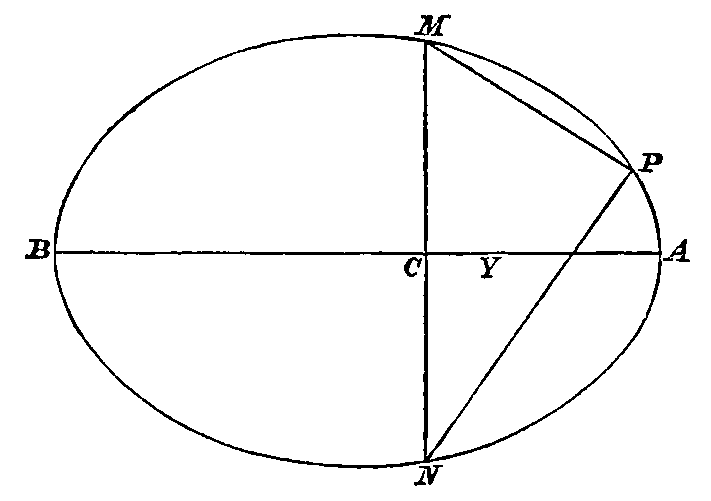
\includegraphics[width=0.6\textwidth]{166.png}
\centering
\end{figure}

Let \(AB\) be the axis of the solid of revolution, \(P\) any point
at its surface, \(MCN\) any double ordinate at right angles to \(AB\).
The note supposes \(P\) to be the vertex of a system of infinitesimal
pyramids, the axes of the pyramids all passing through the
circle generated by the revolution of \(CM\) round \(CA\). The note
concludes that the resultant attraction of these pyramids will be
in the direction \(PC\): this conclusion is obtained by taking the
pyramids in pairs, so that the bases of a pair may be at the opposite
ends of a diameter of the circle; for example, the pyramid
which has \(PM\) for its axis is combined with that which has \(PN\)
for its axis. Now it is quite true that such a pair of pyramids
will exert a resultant attraction along \(PC\), \textit{provided the two pyramids
have equal infinitesimal solid angles:} but this important
%%-----File: 167.png-----%%
condition is practically forgotten in the note. A laborious calculation
is given for determining the resultant attraction of all the
pyramids which have their axes passing through the circle formed
by the revolution of \(CM\) round \(CA\); but this is of no use, because
the bases of all these pyramids will not form a strip of the surface
contained between this circle and an adjacent circle in a parallel
plane, though the note implicitly assumes that they will.

Again, the language of the note seems to suggest that we
are to obtain the attractions exerted on \(P\) by all the circular
elements like that considered, and \textit{add} them together. This would
however be useless; for as these attractions are not all in the
same direction they would have to be resolved according to fixed
directions, and the resolved parts in the \textit{same direction} added.

Again, we are in effect told to obtain the direction of the
resultant attraction of the solid in the following manner: Suppose
\(Y\) a point in \(AB\) such that the attractions on \(P\) of the two segments
into which the solid is divided by a plane through \(Y\) at
right angles to \(AB\) are equal; then \(PY\) is the direction of the
resultant. This statement is certainly untrue. For instance, if
the solid is a sphere, the resultant attraction passes through the
centre; but the two halves formed by cutting the sphere by a
plane do not in general exert equal attractions on a particle at the
surface.

It is incidentally stated, that in the triangle \(PMN\) we have
\({(PM+PN)\,PN}\) greater than \(MN^2\); but this is not necessarily true.

The following extraordinary principle is offered for obtaining
the condition of equilibrium of a mass of fluid in the form of a
solid of revolution. Let \(t\) denote the distance at any point \(P\)
between the bounding surface and a similar surface indefinitely
near, \(f\) the attraction at \(P\), \(y\) the distance of \(P\) from the axis, \(ds\) an
element of the generating curve at \(P\); then \(t\!f\!yds\) is to be constant.
It is sufficient to observe that in the simplest possible case, that
of a sphere, this condition does not hold; for then \(t\) and \(f\) are
constant, but \(yds\) is not constant, except by an arbitrary hypothesis.

The commentators notice the inaccuracy of Newton, on which
I have remarked in Art.\ 33; they assert that gravity at different
%%-----File: 168.png-----%%
places varies inversely as the radius of curvature: ``\dots\ gravitates
in singulis punctis forent reciproce ut radii osculatores curvæ.''
This is untrue; it would make the gravity greatest at the equator
and least at the poles. The fact is that gravity would vary as the
length of the normal between the point and the major-axis.

The commentators having obtained an expression substantially
equivalent to the \(\xp\dfrac{a^3-p^3}{a^3p^3}\), which I have given in Art.\ 35, immediately
proceed to take \(a^3 - r^3\) for the numerator; but this approximation
is not exact to the order which has been retained. I should
add, however, that in their next note there is a correct analytical
investigation of the matter.

\Section
240. We may next advert to a memoir entitled \textit{Determinatio
exactior Graduum Parallelorum Æquatoris et Meridiani \dots\ Auctore
C. N. de Winsheim.} This is contained in the \textit{Commentarii
Academiæ \dots\ Petropolitanæ}, Vol.\ \textsc{xii}.\ which is for 1740; the date
of publication is 1750. The memoir occupies pages 222\dots 240 of
the volume. Here we have Tables giving the lengths of a degree
of the meridian and of a degree of longitude in various latitudes,
for a sphere, and for an oblatum in which the ellipticity is \(\xp\dfrac{1}{183}\).
This ellipticity is found from the Lapland degree of 57438 toises,
and Picard's taken at 57183 toises: see Art.\ 236. Winsheim
ascribes to Euler the rule which he uses for calculating the Tables
with respect to the oblatum.
%%-----File: 169.png-----%%
\Chapter{CHAPTER IX.}
\Subhead{MACLAURIN.}
\Runhead{\textsc{maclaurin.}}

\Section
241. \textsc{Maclaurin's} researches on Attractions first appeared in
his Essay on the subject of the Tides, which gained a prize from
the French Academy in 1740; see Art.\ 232. These researches are
reproduced in an enlarged and improved form, in Maclaurin's work
entitled \textit{A Treatise of Fluxions}, Edinburgh, 1742. The work is
in two quarto volumes; it contains Title Pages, a Dedication to
His Grace the Duke of Argyle and Greenwich on two pages, a
Preface on six pages; then the text on 763 pages, and a page of
Errata: there are \textsc{xl} Plates.

The \textit{Treatise of Fluxions} embodies much of the analysis and
mechanics of the period. Maclaurin touches on the equilibrium
of fluids in his pages 409, 410. We may infer that he had a correct
idea of what we now call the differential equation to the
surface of a homogeneous fluid in equilibrium under given forces.

\Section
242. The part of the \textit{Treatise of Fluxions} with which we are
concerned, occupies pages 522\dots 566, which are in the second
volume.

Maclaurin shews that the attraction of a homogeneous cone
with a given infinitesimal solid angle on a particle at the vertex
varies as the length of the cone; and that the same result holds
for a frustum of the cone; the particle being still supposed at
the vertex of the cone. See his Article 628. Then his Article
629 draws an important inference, which Newton had given in the
first corollary to his Proposition 87. Maclaurin says:

\begin{squote}
The forces with which particles similarly situated with respect to
similar homogeneous solids gravitate towards these solids are as their
Distances from any points similarly situated in the solids, or as any of
%%-----File: 170.png-----%%
their homologous sides. For such solids may be conceived to be resolved
into similar cones, or frustums of cones, that have always their
vertex in the particles, and the gravitation towards these cones, or
frustums, will be always in the same ratio.
\end{squote}

In future, if nothing is said about the density of the attracting
body it is to be understood to be a \textit{homogeneous} body.

\Section
243. Maclaurin shews in his Article 630, that a particle will
be in equilibrium if it is placed at any point within the hollow
part of a shell, the surfaces of which are concentric, similar, and
similarly situated ellipsoids of revolution; the demonstration is
the same as Newton's: see Art.\ 13.

\Section
244. Let the attraction of an ellipsoid of revolution on any
constituent particle be resolved into two components, one perpendicular
to the axis, and the other parallel to the axis; then the
former component varies as the distance of the particle from the
axis, and the latter component varies as the distance from the
plane of the equator. Maclaurin demonstrates these theorems,
first formally stated by himself, by a beautiful geometrical process:
see his Articles 631\dots 634.

Clairaut preserves the essence of Maclaurin's demonstration:
he says, ``Cette méthode m'a paru si belle et si savante\dots'': see
\textit{Figure de la Terre}, pages 157\dots 170.

Suppose that \(\lambda\) denotes the constant coefficient for the component
attraction parallel to the axis, and \(\mu\) the constant coefficient
for the component perpendicular to the axis; then, by some general
reasoning, Maclaurin arrives at the result that the product of \(\lambda\)
into the square of the polar axis is less or greater than the product
of \(\mu\) into the square of the equatorial axis according as the ellipsoid
of revolution is oblate or oblong: see his Article 635.

\Section
245. Let there be an ellipsoid of revolution; let \(2a\) be the
equatorial diameter, and \(2b\) the polar diameter. Suppose the
ellipsoid to be fluid; and besides the mutual attractions let there
be at every point any other force perpendicular to the axis varying
as the distance from the axis, and any other force parallel to the
axis varying as the distance from the plane of the equator:
%%-----File: 171.png-----%%
the necessary and sufficient condition for equilibrium is that \(a\)
must be to \(b\), as the resultant force at the pole is to the resultant
force at the equator. This theorem can be demonstrated immediately
by the aid of the well-known equations for the equilibrium
of a fluid. Maclaurin, however, was not in possession of these
equations; so that he adopted a different method. He says in his
Article 636:

\begin{squote}
To demonstrate this proposition fully, we shall shew, 1. That the
force which results from the attraction of the spheroid and those extraneous
powers compounded together acts always in a right line perpendicular
to the surface of the spheroid.\ 2. That the columns of the
fluid sustain or ballance each other at the center of the spheroid. And
3. That any particle in the spheroid is impelled equally in all directions.
\end{squote}

He gives his demonstrations in his Articles 637, 638, 639.

Maclaurin then was in this position: there was as yet no theory
of fluid equilibrium which indicated what conditions were \textit{sufficient},
so he shews that all the conditions which had then been recognised
as \textit{necessary} for equilibrium would be satisfied in the case
supposed. He easily demonstrates the first condition, which,
as we know, was given by Huygens: see Art.\ 53. Maclaurin's
second condition is a particular case of his third, and was given
by Newton: see Art.\ 23. The meaning which Maclaurin attaches
to his third condition is the following: Take any definite point
within the mass; draw from this point a straight line to the surface
\textit{in any direction}; let this straight line be the axis of a column
of given infinitesimal section: then the attraction on the column
resolved along the column, is independent of the direction.
Maclaurin, however, only demonstrates this for the case in which
the direction is in the \textit{meridian plane} of the definite point; he
says that ``in like manner, it is shewn'' that the result is true for
columns not in the meridian plane: but it is not obvious how
he would have proceeded. The result can be obtained very easily
by modern methods.

Maclaurin's third condition is thus an extension of Newton's
principle of balancing columns, \textit{any point} being taken instead of
the centre, at which the balancing is to hold. Huygens had briefly
alluded to this extension: see Art.\ 55.
%%-----File: 172.png-----%%

\Section
246. This extension of Newton's principle of balancing columns
seems to have been considered important at the time. D'Alembert
says on page 14 of his \textit{Essai \dots\ de la Résistance des Fluides}:

\begin{squote}
Quoique le Principe de l'équilibre des Canaux rectilignes, soit comme
l'on voit, une conséquence très-naturelle de la pression des Fluides en
tout sens; cependant je dois reconnoître ici, que feu \textit{M. Maclaurin} est
le premier qui ait fait usage de ce Principe, et qui l'ait appliqué à la
recherche importante de la Figure de la Terre. Voyez son \textit{Traité des
Fluxions}, art.\ 639, et son Traité \textit{de Causa Fluxûs et Refluxûs maris},
Paris, 1740.
\end{squote}

See also D'Alembert's \textit{Traité \dots\ des Fluides}, second edition,
page 49.

\Section
247. In Maclaurin's Article 637, we have the important result
which we have noticed in our account of Stirling; namely, that
when rotating fluid in the form of an oblatum is in relative
equilibrium the gravity at any point of the surface varies \textit{exactly}
as the length of the normal between the point and the plane of
the equator; see Art.\ 153. This result had however been communicated
to the Royal Society by Simpson, in 1741, before the
publication of Maclaurin's \textit{Fluxions}: see the preface to Simpson's
\textit{Mathematical Dissertations}. Simpson seems to claim priority for
himself; but he overlooks the fact that Maclaurin had previously
given the result in his prize essay on the Tides: it is the \textit{Theorema
Fundamentale} of the essay.

It follows immediately from conic sections that instead of the
gravity varying as the length of the normal between the point and
the plane of the equator, we may take the length of the normal
between the point and the axis of revolution.

\Section
248. Maclaurin, in his Article 640, states the conclusions
which he had thus demonstrated respecting the problem of Art.\ 245.
Among them we may observe that he says, surfaces similar, similarly
situated, and concentric with the bounding surface ``will be
level surfaces at all depths.''

This is the first mention I find of \textit{level} surfaces; the essential
property of a level surface is that the resultant force at any point
of the surface is in the direction of the normal to the surface at
that point.
%%-----File: 173.png-----%%

D'Alembert in his \textit{Essai \dots\ de la Résistance des Fluides}, page 202,
says:

\dots\ \textit{M. Maclaurin}, le premier qui ait parlé de ces couches \dots\ auxquelles
la pesanteur est perpendiculaire, et qu'il appelle \textit{surfaces de
niveau}\dots.

\Section
249. Maclaurin now applies the results obtained for the
general problem of Art.\ 245 to the particular case of the relative
equilibrium of a revolving fluid.

He says in his Article 641:

\begin{squote}
It appears therefore that if the earth, or any other planet, was
fluid and of an uniform density, the figure which it would assume in
consequence of its diurnal rotation, would be accurately that of an
oblate spheroid generated by an ellipsis revolving about its second axis,
as Sir \textsc{Isaac Newton} supposed.
\end{squote}

Here, Maclaurin says more than he was justified in saying;
he had not proved that the planet \textit{would} assume the form of an
oblatum, but only that this form is \textit{a} form of relative equilibrium.
See Art.\ 168.

The proposition really investigated was first established \textit{exactly}
by Maclaurin; as we have stated, Stirling and Clairaut had given
approximate investigations of it: see Arts.\ 156 and 163.

\Section
250. Maclaurin now proposes to calculate the attraction of an
ellipsoid of revolution at the pole or at the equator. He begins
with a lemma which forms his Article 642. Let a slice of an
attracting body be formed by two planes, both containing the
attracted particle, and inclined to each other at an infinitesimal
angle: then the lemma shews how to calculate the attraction of
the slice resolved along a given direction in one of the planes.

\Section
251. Before discussing the attraction of an ellipsoid of revolution,
Maclaurin considers that of a sphere in his Article 643.
The following general result is obtained: Let \(C\) be the centre of
a circle, \(P\) any external point in the plane of the circle. From \(P\)
draw any straight line cutting the circumference of the circle at
\(L\) and \(M\); and let a solid be formed by the revolution round \(PC\)
of the smaller segment of the circle cut off by \(LM\). Then the
attraction of this solid on a particle at \(P\) varies as \(\xp\dfrac{(LM)^3}{(PC)^2}\).
%%-----File: 174.png-----%%

This may be easily verified by the aid of the general expression
given in Art.\ 4. The formula is very remarkable; it does not
involve the radius of the sphere; that is, if \(LM\) is constant,
we get the attraction constant whatever may be the value of the
radius. The result was generalised by Legendre, as we shall see,
in his third memoir.

\Section
252. Maclaurin then in his Articles 644\dots 647 investigates
accurate expressions for the attraction of any ellipsoid of revolution
on a particle at the pole or at the equator. The investigations
are conducted in the manner of the time by representing the
attractions by the areas of certain curves, and finding the areas by
the method of fluents. The results agree with those obtained by
analysis, and presented in modern works on Statics. Maclaurin's
processes are remarkable specimens of ingenuity, considering the
date of their publication; but they will not be very interesting
to a modern reader.

\Section
253. Maclaurin says in his Article 647:

\begin{squote}
\dots\ What has been shown concerning the gravity at the pole \dots\ agrees
with what was advanced long ago by Sir \textsc{Isaac Newton} and Mr.\ \textsc{Cotes},
who contented themselves with an approximation in determining the
gravity at the equator, which is exact enough when the spheroid differs
very little from a sphere. The approximations proposed lately for this
purpose, \textit{Phil.\ Trans.}\ N. 438 and 445, are more accurate; and Mr.\
\textsc{Stirling} after determining the gravity at the equator by a converging
series, since found that the sum of the series could be assigned from the
quadrature of the circle.
\end{squote}

I do not know what is intended by the reference to Mr Cotes.
Of course Cotes, as editor of the \textit{Principia}, may be supposed to
have accepted some of the responsibility which would otherwise
have fallen on Newton alone: but Maclaurin's words seem to imply
that Cotes had made some investigations of his own. The paper
in the \textit{Philosophical Transactions}, Number 438, is that by Stirling,
of which we gave an account in Chapter V.; and the paper in the
\textit{Philosophical Transactions}, Number 445, is that by Clairaut, of
which we gave an account in Arts.\ 163\dots 166. I do not know
what Maclaurin means by the words ``and Mr Stirling \dots\ circle.''

This passage from Maclaurin was quoted, and the difficulty
%%-----File: 175.png-----%%
as to its meaning noticed, by the late Sir J. W. Lubbock: see
page 24 of his work cited in Art.\ 233.

I do not know whether the conjecture may be considered
plausible that Maclaurin wrote \textit{Stirling} by mistake for \textit{Simpson}.
It appears from the preface to Simpson's \textit{Mathematical Dissertations}
that his researches on the Figure of the Earth were read to
the Royal Society in March or April, 1741; and what Maclaurin
says with respect to Mr Stirling is not unsuitable to the investigation
we find in Simpson's work, except that Simpson does not
restrict himself to a point at the equator, but takes any point on
the surface.

\Section
254. Maclaurin proceeds in his Articles 648\dots 652 to one of
the most important of his investigations, remarkable as forming
a large part of the theorem which now usually bears the name of
Ivory, though it was substantially first demonstrated by Laplace.
Maclaurin's theorem is as follows in modern language: Let
there be two confocal ellipses, and let them both revolve round
their major-axes, or round their minor-axes, so as to generate
two ellipsoids of revolution: then the attractions of the two
ellipsoids on the same particle external to both will be as the
volumes, provided the particle be on the prolongation of the axis
of revolution, or in the plane of the equator. Two such ellipsoids
may be called confocal ellipsoids of revolution. Legendre shewed
that the theorem was true for any position of the external particle.

The general theorem demonstrated by Laplace is as follows:
If there be two confocal ellipsoids, that is, ellipsoids which have
the same foci for their principal sections, their attractions on any
particle external to both will be as their volumes, that is, will be
the same in direction, and in amount will be as their volumes. The
simplest statement in modern language is this: The potentials of
confocal ellipsoids on a given external particle are as their volumes.

Maclaurin in a later Article, namely 653, gave so much of
this general theorem as consists with the limitation that the
particle must be on the prolongation of an axis of the ellipsoids.
Ivory merely supplied an improved form of demonstration to
Laplace's theorem; and combined it with the fact that inside
an ellipsoid, along any radius-vector, the attraction varies as the
distance from the centre.
%%-----File: 176.png-----%%

Maclaurin's Articles 648 and 649 contain his demonstration for
the case in which the external particle is on the prolongation of
the axis of revolution. These Articles may be read without difficulty,
apart from Maclaurin's other investigations, by those who
are desirous of seeing a specimen of his own processes.

\Section
255. It is easy to translate into modern language the essence
of Maclaurin's demonstration.

Let \(2a\) and \(2b\) be the axes of an ellipse; let the ellipse revolve
about the axis of length \(2a\), and thus generate an ellipsoid of revolution:
required the attraction of the ellipsoid on a particle which
is on the prolongation of the axis of revolution at a distance \(c\) from
the centre.

Let \(r\) be the distance of the attracted particle from any point
of the ellipsoid; let \(\theta\) be the angle between \(r\) and the axis of
revolution. We see in the usual way that the attraction is found
by integrating with respect to \(r\) and \(\theta\) the expression
\[
\frac{2\pi r dr\,r\sin \theta \cos \theta d\theta} {r^2}\text{.}
\]

Integrate with respect to \(r\) and we obtain
\[
2\pi(r_{2}-r_{1}) \sin \theta \cos \theta\,d\theta,
\]
where \(r_{2}\) and \(r_{1}\) are respectively the greatest and the least values
of the radius-vector drawn from the attracted particle to the ellipsoid
at the inclination \(\theta\) to the axis of revolution.

Hence \(r_{2}\) and \(r_{1}\) are the roots of the quadratic equation
\[
\frac{(r \cos \theta - c)^2}{a^2} + \frac{r^2 \sin^2 \theta}{b^2} = 1,
\]
and thus we shall find that
\[
\begin{aligned}
r_{2} - r_{1} &= \frac{2ab \xsurd(b^2 \cos^2 \theta + a^2 \sin^2 \theta - c^2 \sin^2 \theta)} {b^2 \cos^2 \theta + a^2 \sin^2 \theta}\\
&=\frac{2ab \xsurd\{b^2 + (a^2 - b^2 - c^2) \sin^2 \theta\}}{b^2 + (a^2 - b^2) \sin^2 \theta}\text{.}
\end{aligned}
\]

Now let there be a second ellipsoid of revolution, having the
foci of its generating ellipse in the same position as before; and
%%-----File: 177.png-----%%
let accented letters be used to denote the analogous quantities;
so that
\[
{r_2}' - {r_1}' = \frac{2a'b' \xsurd\{b'^2 + (a'^2 - b'^2 - c^2) \sin^2 \theta'\}} {b'^2 + (a'^2 - b'^2) \sin^2 \theta'}\text{.}
\]

Since the foci of the generating ellipses are coincident, we
have \({a^2 - b^2 = a'^2 - b'^2}\), whether the ellipsoids are oblate or oblong.
Assume \(\sin \theta' = \xp\dfrac{b'}{b} \sin \theta\); then we see that
\[
\frac{{r_2}'-{r_1}'} {r_{2}-r_{1}} = \frac{a'}{a};
\]
and therefore
\[
\frac{({r_2}'-{r_1}') \sin \theta' \cos \theta' d\theta'} {(r_{2}-r_{1}) \sin \theta \cos \theta d\theta} = \frac{a'b'^2} {ab^2}\text{.}
\]

Thus the attractions of the corresponding elements of the two
ellipsoids resolved along the direction of the axis of revolution are
in the same proportion as the volumes of the ellipsoids; and so
the resultant attractions of the whole ellipsoids will be in that
proportion.

It will be observed that on our assumption \({r_2}'-{r_1}'\) and \(r_{2}-r_{1}\)
\textit{vanish together}; so that our elements \textit{always} correspond. If the
density of one ellipsoid is not the same as the density of the
other, then the attractions will of course be in the ratio of the
\textit{masses} instead of the ratio of the \textit{volumes}. This remark will be
obviously applicable in some subsequent Articles.

Maclaurin's own investigation in his Art.\ 648 applies to his
figure 292, which is drawn for an oblatum; but the figure may be
drawn for an oblongum, and it will be found that the investigation
is equally applicable. In Maclaurin's investigation the point
\(P\) is \textit{on} the larger ellipsoid; but still this involves the result in as
general a form as we have stated it.

\Section
256. Maclaurin's Article 650 consists of three sentences; it
would have been advantageous, for the sake of clearness, if they
had been printed as three distinct paragraphs: the last sentence
most certainly should have been separated from the others.

In the first sentence Maclaurin gives an expression for the
attraction of an oblatum on an external particle which is situated
%%-----File: 178.png-----%%
on the axis of revolution: this follows from his former results,
which we have noticed in Arts.\ 252 and 255.

In the second sentence Maclaurin gives the corresponding expression
for the attraction of an oblongum.

The third sentence is very remarkable. It has been shewn
that the attraction of a homogeneous ellipsoid of revolution on
an external particle which is situated on the axis of revolution,
varies as the mass, so long as the generating ellipse keeps its foci
fixed; now suppose an ellipsoid of revolution, not homogeneous,
but made up of shells, each shell being bounded by confocal
ellipsoids of revolution, and the density being uniform throughout
each shell, but varying in any manner from shell to shell: then
the attraction of this heterogeneous ellipsoid on an external
particle situated on the axis of revolution is to the attraction of a
homogeneous ellipsoid of the same size as the mass of the former
is to the mass of the latter. This is the first appearance of these
\textit{confocal} shells, which play an important part in modern works on
Attraction.

\Section
257. Maclaurin now proceeds in his Articles 651, 652 to the
case in which the attracted external particle is in the plane of the
equator of the attracting ellipsoid of revolution. He uses a most
ingenious artifice by which this case is made to depend on that
already considered, in which the attracted particle is on the
prolongation of the axis of revolution. We will translate his
process into modern language.

Let the equation to one ellipsoid of revolution be \(\xp\dfrac{x^2}{a^2} + \xp\dfrac{y^2+z^2}{c^2} = 1\),
and the equation to another \(\xp\dfrac{x^2}{a'^2} + \xp\dfrac{y^2+z^2}{c'^2} = 1\). Suppose the generating
ellipses to have the same foci; then, whether the ellipsoids
are oblate or oblong, \(a^2 - c^2 = a'^2 - c'^2\).

Suppose the second ellipsoid to be the larger. We propose to
compare the attractions of these ellipsoids on a particle which is
\textit{on} the equator of the larger ellipsoid; the co-ordinates of the
particle may be taken to be \(0\), \(0\), \(c'\). We shall shew that the
attractions of the ellipsoids are as their volumes.
%%-----File: 179.png-----%%

Let \(C\) denote the centre of the ellipsoids, and \(P\) the position of
the attracted particle.

Let two planes pass through \(CP\), and make with the axis of \(y\)
the angles \(\theta\) and \(\theta + \delta\theta\), respectively: we will call these planes the
\textit{first pair of planes}. Let two other planes pass through \(CP\), and
make with the axis of \(y\) the angles \(\theta'\) and \(\theta' + \delta\theta'\) respectively: we
will call these planes the \textit{second pair of planes}. The volume
comprised between the first pair of planes and the first ellipsoid
we will call the \textit{element of the first ellipsoid}; the volume comprised
between the second pair of planes and the second ellipsoid we will
call the \textit{element of the second ellipsoid}: each element then consists
of \textit{two} wedge-shaped slices. We shall shew that when a suitable
relation is made to hold between \(\theta\) and \(\theta'\), the attractions of these
elements on the particle at \(P\) are as their volumes.

The relation between \(\theta\) and \(\theta'\) is found by assuming that the
ellipses which form the boundaries of the elements shall be \textit{confocal}.
Thus we have \(r^2-c^2 = r'^2-c'^2\),
where
\[
r^2 = \frac{a^2c^2}{a^2 \cos^2 \theta + c^2 \sin^2 \theta}\text{, and }r'^2 = \frac{a'^2c'^2}{a'^2 \cos^2 \theta' + c'^2 \sin^2 \theta'}\text{.}
\]

Since \(a^2 - c^2 = a'^2 - c'^2\), we obtain
\hypertarget{257:1}{\[
\frac{c^2 \sin^2 \theta}{a^2 \cos^2 \theta + c^2 \sin^2 \theta} = \frac{c'^2 \sin^2 \theta'}{a^2 \cos^2 \theta' + c'^2 \sin^2 \theta'}\text{:}
\]}
this is the relation between \(\theta\) and \(\theta'\). It is obvious that to the
limits \(0\) and \(\xp\dfrac{\pi}{2}\) for \(\theta\) correspond the same limits for \(\theta'\).

Suppose now that a solid were formed by the revolution round
\(CP\) of an ellipse having \(C\) for centre, \(2c\) for the axis of revolution,
and \(2r\) for the other axis. Let \(F\) denote the attraction of this
solid on the particle at \(P\). Then it is obvious that ultimately the
attraction of the \textit{element of the first ellipsoid} on the particle is
\(\xp\dfrac{\delta\theta}{\pi} F\).

Also suppose that a solid were formed by the revolution round
\(CP\) of an ellipse having \(C\) for centre, \(2c'\) for the axis of revolution,
and \(2r'\) for the other axis. Let \(F'\) denote the attraction of
this solid on the particle at \(P\). Then it is obvious that ultimately
%%-----File: 180.png-----%%
the attraction of the \textit{element of the second ellipsoid} on the particle
is \(\xp\dfrac{\delta\theta'}{\pi} F'\).

Therefore if \(f\) and \(f'\) denote the attractions of the elements, we
have
\[\frac{f}{f'} = \frac{F\ldot\delta\theta}{F'\ldot\delta\theta'}.\]

Now, as we have seen in Art.\ 255, Maclaurin had shewn that
\[\dfrac{F}{F'} = \frac{r^2 c }{ r'^2 c'};\]
therefore
\[\frac{f}{ f'} = \frac{r^2 c \delta\theta }{r'^2 c' \delta\theta'}.\]
But \(r^2\delta\theta\) represents the area intercepted by the first pair of planes
from the ellipse \(\xp\dfrac{x^2}{a^2} + \xp\dfrac{y^2}{c^2} = 1\); and \(r'^2\delta\theta'\) represents the area intercepted
by the second pair of planes from the ellipse \(\xp\dfrac{x^2}{a'^2} + \xp\dfrac{y^2}{c'^2} = 1\).
Thus we see that \(f\) is to \(f'\) as the volume of the element of the
first ellipsoid is to the volume of the element of the second ellipsoid.
And as this proportion holds for every corresponding pair
of elements it holds for the entire ellipsoids; which is what we
had to demonstrate.

\Section
258. The process may be easily extended to the case in which
the ellipsoids are not of revolution, as Maclaurin himself indicates
in his Article 653.

Let the equations to the ellipsoids be
\[\frac{x^2}{a^2} + \frac{y^2}{b^2} + \frac{z^2}{c^2} = 1,\quad \frac{x^2}{a'^2} + \frac{y^2}{b'^2} + \frac{z^2}{c'^2} = 1;\]
and let the principal sections of the ellipsoids be confocal, so that
\[c^2 - a^2 = c'^2 - a'^2\text{, and }c^2 - b^2 = c'^2 - b'^2.\]

The relation between \(\theta\) and \(\theta'\) will then be found from the
condition
\[r^2 - c^2 = r'^2 - c'^2,\]
where
\[r^2 = \frac{a^2 b^2}{ a^2 \cos^2\theta + b^2 \sin^2\theta}\text{, and }r'^2 = \frac{a'^2 b'^2}{ a'^2 \cos^2\theta' + b'^2 \sin^2\theta'}.\]

As before, we shall find that to the limits 0 and \(\xp\dfrac{\pi}{2}\) for \(\theta\) correspond
%%-----File: 181.png-----%%
the same limits for \(\theta'\). Then the investigation and the result
will be as in the preceding Article.

\Section
259. Thus in the attraction of homogeneous ellipsoids
Maclaurin's position was as follows: he solved completely the
problem of the attraction of an ellipsoid of revolution on any
internal particle; and with respect to an external particle, he
obtained for ellipsoids, not necessarily of revolution, the theorem
of Laplace, so far as relates to a particle on the prolongation of \textit{an
axis} of the ellipsoids. All this was \textit{exactly} demonstrated.

Maclaurin states also something more as approximately true in
his Article 654. The statement amounts to this, that the theorem
of Art.\ 254 is true ``either accurately or nearly when the spheroids
differ little from spheres,'' when the attracted particle has \textit{any}
position. He gives no detail as to the investigation of this result;
but merely says it may be deduced from his Article 653. We
know now that the theorem is exact and not merely an approximation;
and, as we have stated, the demonstration was first
given by Legendre, and the theorem is a part of Laplace's general
theorem.

\Section
260. The extent to which Maclaurin carried his investigations
was underestimated by many of the succeeding writers. He was
supposed to have merely \textit{enunciated} the result which we have
noticed in Art.\ 258, whereas he really \textit{demonstrates} it: he says
``it will appear in the same manner\dots'' and it is clear from an
examination of his context that this is the case. The erroneous
account will be found in the following places: D'Alembert,
\textit{Opuscules Mathématiques}, Vol.\ \textsc{vi}.\ 1773, page 243; Lagrange,
Berlin \textit{Mémoires} for 1775, page 279; Laplace, \textit{Théorie \dots\ de la
Figure elliptique des Planetes}, 1784, page 96; Legendre, \textit{Mémoires
\dots\ par divers Savans}, Vol.\ \textsc{x}.\ 1785, page 412. Laplace, \textit{Mécanique
Céleste}, Vol.\ \textsc{v}.\ page 9. Plana in Crelle's \textit{Journal für \dots\ Mathematik},
Vol.\ \textsc{xx}.\ page 190. According to the catalogues of booksellers,
it appears that Maclaurin's \textit{Fluxions} was translated into
French, so that there is less excuse for the error. I suppose that
D'Alembert went astray, and the others followed in succession
without examination. Chasles is correct; he says that Maclaurin
%%-----File: 182.png-----%%
did demonstrate his theorem, and he points out the error in this
matter made by D'Alembert, Lagrange, Legendre, and others:
see the \textit{Mémoires \dots\ par divers Savants}, Vol.\ \textsc{ix}.\ 1846, page 632.
The error is also noticed by Dr F. Grube in a paper in the
\textit{Zeitschrift für Mathematik und Physik}, Vol.\ \textsc{xiv}.\ Leipsic, 1869,
page 272.

On the other hand, some recent English writers have gone to
the opposite extreme, and given to Maclaurin more than his due,
by ascribing to him in effect the entire theorem called Ivory's, but
more strictly Laplace's; see \textit{Natural Philosophy}, by Thomson and
Tait, Vol.\ \textsc{i}.\ page 392, and Routh's \textit{Rigid Dynamics}, 2nd edition,
page 421.

\Section
261. It will be convenient to give the results obtained by
Maclaurin as to the attraction of an oblatum on an external particle
which is in the plane of the equator, or on the prolongation
of the axis of revolution.

\begin{figure}[!ht]
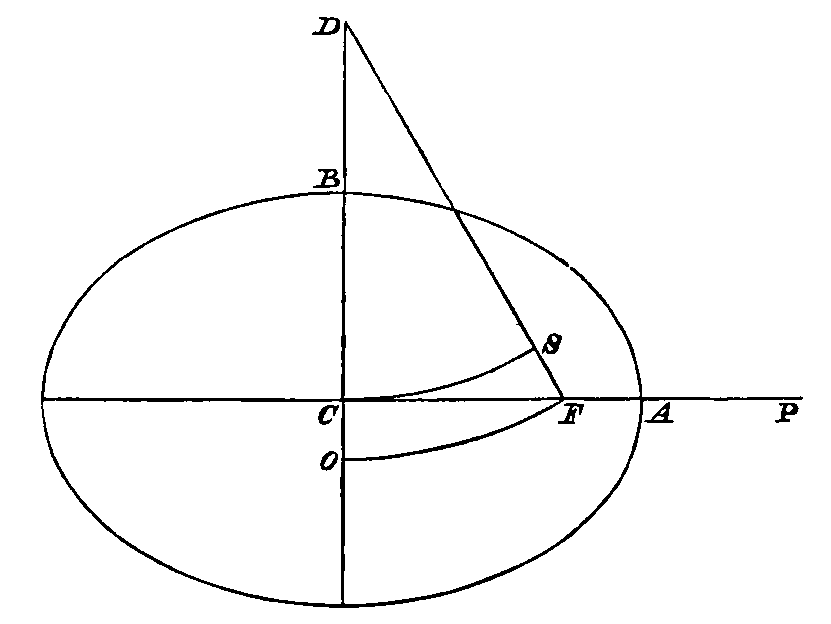
\includegraphics[width=0.65\textwidth]{182.png}
\centering
\end{figure}

Let \(P\) be the position of an external particle which is in the
plane of the equator. Let \(F\) be the focus of the section of the
oblatum made by the plane which contains \(P\) and the axis of
revolution. Let \(C\) be the centre, \(CA\) and \(CB\) the semi-axes of
the section. With \(F\) as centre, and a radius equal to \(CP\),
describe a circle cutting \(CB\) produced at \(D\). With \(D\) as centre,
and \(DF\) as radius, describe the arc \(FO\), and with \(D\) as centre and
\(DC\) as radius, describe the arc \(CS\).
%%-----File: 183.png-----%%

Then Maclaurin obtains for the attraction on a particle at \(P\)
the expression
\[\frac{2\ldot CB\ldot CA^2 }{CF^3} \times \frac{\text{area } FCO}{CP}.\]

And for the attraction on a particle at the point \(D\) on the
prolongation of the axis of revolution, he obtains the expression
\[\frac{2\ldot CB\ldot CA^2}{CF^3} \times (CF - CS).\]

If we multiply these expressions by \(2\pi\rho\), where \(\rho\) denotes the
density, they will be found to agree with those given in modern
works on Statics when we suppose \(P\) to be on the surface; and
the case where \(P\) is not on the surface may be deduced from that
where \(P\) is on the surface, by Maclaurin's theorem of Art.\ 254.
The presence or absence of such a factor as \(2\pi\) merely depends
on the choice we have made of the unit of attraction.

Put \(a\) for \(CA\), and \(ae\) for \(CF\); also put \(r\) for \(CP\) in the first
expression, and \(r\) for \(CD\) in the second; then, introducing the
factor \(2\pi\rho\), our expressions become:
\[\frac{2\pi\rho\xsurd(1-e^2)}{e^3}\left\{ r \sin^{-1} \frac{ea}{r} - \frac{ae \xsurd(r^2 - e^2a^2)}{ r} \right\}\tag{1},\]
and
\[\frac{4\pi\rho \xsurd(1-e^2)}{e^3}\left\{ ea - r \tan^{-1} \frac{ea}{r}\right\} \tag{2},\]
so that (1) applies to the particle in the plane of the equator,
and (2) to the particle on the prolongation of the axis of
revolution.

It will be useful for us to collect here some obvious deductions
from (1) and (2).

The attraction at the equator is obtained by putting \(a\) for \(r\)
in (1); and the attraction at the pole is obtained by putting
\(a \xsurd(1-e^2)\) for \(r\) in (2).

Let \(x\) and \(y\) be the co-ordinates of any point \textit{on the surface} of
the oblatum, measured from the origin \(C\) parallel to \(CA\) and \(CB\)
respectively. Then, by Art.\ 244, combined with the values of the
attraction at the equator and at the pole, to which we have just
alluded, we obtain for the attractions at the point \((x,y)\), resolved
parallel to \(CA\) and \(CB\) respectively,
%%-----File: 184.png-----%%
\[\frac{2\pi\rho \xsurd(1-e^2)}{ e^3} \left\{ \sin^{-1}e - e\xsurd(1-e^2) \right\} x,\]
and
\[\frac{4\pi\rho}{e^3} \left\{ e - \xsurd(1-e^2) \sin^{-1}e \right\} y.\]

If we expand these and neglect \(e^4\) and higher powers of \(e\) we
obtain respectively
\[\frac{4\pi\rho}{3} \left(1 - \frac{e^2}{5}\right)x\quad\text{and}\quad \frac{4\pi\rho}{3} \left(1 + \frac{2e^2}{5}\right)y.\]

By expanding their second factors in powers of \(e\), the expressions
(1) and (2) become respectively
\[\frac{4\pi\rho}{3} \xsurd(1-e^2)\left\{\frac{ a^3}{r^2} + \frac{3e^2}{10} \frac{a^5}{r^4} + \frac{9e^4}{56} \frac{a^7}{r^6} + \ldots \right\},\]
and
\[\frac{4\pi\rho}{3} \xsurd(1-e^2) \left\{ \frac{a^3}{r^2} - \frac{3e^2}{5}\frac{ a^5}{r^4} + \frac{3e^4}{7}\frac{ a^7}{r^6} + \ldots \right\}.\]

In the expressions (1) and (2) change \(a\) into \(a + \delta a\), and subtract
the original values; thus we obtain the attraction of a shell
bounded by similar, similarly situated, and concentric oblata, on
an external particle in the plane of the equator or on the prolongation
of the axis: supposing \(\delta a\) so small that all powers beyond
the first may be neglected, the results are respectively
\[\frac{4\pi\rho \xsurd(1-e^2)}{e^3} \frac{e^2 a^2}{r \xsurd(r^2-e^2 a^2)} e \delta a,\]
and
\[\frac{4\pi\rho \xsurd(1-e^2)}{e^3} \frac{e^2 a^2}{ r^2 + e^2 a^2} e \delta a.\]

Maclaurin, subsequently, in his Articles 668 and 669, gives
without demonstration, in a geometrical form, results which are
equivalent to these.

\Section
262. Maclaurin, in his Article 655, applies his results to find
the condition for the relative equilibrium of an oblatum of fluid
rotating round the minor axis. Let \(a\) be the semi-axis major, and
\(e\) the excentricity. Let \(X\) denote the attraction at the equator,
and \(Y\) the attraction at the pole. Then we obtain \(X\) by putting
\(a\) for \(r\) in the expression (1) of Art.\ 261, and we obtain \(Y\) by
putting \(a\xsurd(1-e^2)\) for \(r\) in the expression (2). Thus we find
%%-----File: 185.png-----%%
\[\frac{Y}{X} = \frac{2\{e - \xsurd(1-e^2) \sin^{-1}e\}} {\sin^{-1}e - e\xsurd(1-e^2)}.\]

Suppose that \(jX\) denotes the value of the centrifugal force at
the equator; then for relative equilibrium we must have, by
Art.\ 245,
\[\frac{X-jX}{Y} = \xsurd(1-e^2);\]
therefore
\[j =\frac{ X - Y\xsurd(1-e^2)}{X}.\]

Put for \(\xp\dfrac{Y}{X}\) its value, and this becomes
\[j = \frac{3\{ \sin^{-1}e - e\xsurd(1-e^2)\} - 2e^2 \sin^{-1}e}{ \sin^{-1}e - e\xsurd(1-e^2)}.\]

These expressions are exact. By approximation we obtain
\[\frac{Y}{X} = \frac{1 + \dfrac{2}{5} e^2 + \dfrac{8}{35} e^4 + \dfrac{16}{105} e^6 + \ldots}{1 + \dfrac{3}{10} e^2 + \dfrac{9}{56} e^4 + \dfrac{5}{48} e^6 + \ldots },\]
\[j =\frac{\dfrac{2}{5} e^2 + \dfrac{9}{35} e^4 + \dfrac{5}{28} e^6 + \ldots}{1 + \dfrac{3}{10} e^2 + \dfrac{9}{56} e^4 + \dfrac{5}{48} e^6 + \ldots }.\]

Maclaurin gives these approximations as far as \(e^4\) inclusive.

By reversion of series we obtain
\[e^2 = \frac{5j}{2} - \frac{15j^2}{7} + \ldots\text{;}\]
so that when the oblatum differs very little from a sphere we
may take
\[e^2 = \frac{\dfrac{5j}{2}}{1 + \dfrac{6j}{7}}.\]

Maclaurin then says, ``in this case the excess of the semi-diameter
of the equator above the semiaxis is to the mean semi-diameter
nearly as'' \(5j\) is to \(4 - \xp\dfrac{11j}{7}\). By the \textit{mean semi-diameter}
%%-----File: 186.png-----%%
he intends half the sum of the polar and equatorial radii. Taking
1 for the equatorial radius, we have \(\xsurd(1-e^2)\) for the polar
radius; then the ratio of the difference to the half-sum is
expressed exactly by \(\xp\dfrac{2\,\{1 - \xsurd(1-e^2)\}}{1 + \xsurd(1-e^2)}\).

If we wish to be correct only to the first power of \(e^2\) this
becomes \(\xp\dfrac{e^2}{2}\).

If we wish to be correct to the second power of \(e^2\) this becomes
\(\xp\dfrac{e^2\left(1+\dfrac{e^2}{4}\right)}{2-\dfrac{e^2}{2}}\). We might use other forms which would coincide
with this as far as the second power of \(e^2\). For instance, we have
the ratio exactly equal to \(\xp\dfrac{2e^2}{\{1+\xsurd(1-e^2)\}^2}\), and thus to the order
of \(e^4\) we get \(\xp\dfrac{2e^2}{4-2e^2}\); and then we may put this to the same
order in the form \(\xp\dfrac{e^2}{2}\left(1+\dfrac{e^2}{2}\right)\).

Taking the form \(\xp\dfrac{2e^2}{4-2e^2}\) and putting \(\xp\dfrac{\dfrac{5j}{2}}{1+\dfrac{6j}{7}}\) for \(e^2\), we obtain
with Maclaurin \(\xp\dfrac{5j}{4-\dfrac{11j}{7}}\).

\Section
263. Maclaurin shews how the value of \(e^2\) for the Earth,
supposed homogeneous, may be deduced from the measured
length of a degree of the meridian in any latitude, and the
measured length of the pendulum which vibrates in a given time
in that latitude: see his Articles 656\dots 658. He shews in his
Article 657 that the radius of curvature in the ellipse varies as
the cube of the length of the normal terminated by the major
axis; he was, probably, the first to demonstrate this: see the \textit{Mécanique
Céleste}, Vol.\ \textsc{v}.\ page 6.

Maclaurin also shews how the value of \(e^2\) may be deduced
from the distance and the periodic time of a satellite revolving
in the plane of the equator: see his Articles 659 and 660.
%%-----File: 187.png-----%%

Maclaurin in his Articles 661\dots 665 obtains numerical results
with respect to the Earth, supposed homogeneous. He does not
determine strictly the value of the quantity we denote by \(j\); but he
finds \(\xp\dfrac{1}{289.3}\) as the value of the ratio of the centrifugal force at
the equator to the force of gravity at Paris, and \(\xp\dfrac{1}{287.8}\) as the
value of the ratio of the centrifugal force at the equator to the force
of gravity at the Polar circle. For the ratio of the axes of the
Earth he obtains a result practically equivalent to Newton's value
of 230 to 229.

Maclaurin shews, however, that this result is not consistent
with that obtained by means of the observations of pendulums in
various latitudes; nor with that obtained from the measured
lengths of a degree of the meridian in France and in Lapland:
both these methods gave for the ellipticity a larger value than \(\xp\dfrac{1}{230}\).
We have now more accurate observations and measurements
than those accessible to Maclaurin; and we know that the true
value of the ellipticity is about \(\xp\dfrac{1}{300}\).

\Section
264. Maclaurin then proposes to treat the Earth as not uniform
in density. In his Article 666 he supposes that there is
\textit{more} matter at the centre than is consistent with the hypothesis
of uniform density; and in his Article 667 he supposes that there
is \textit{less} matter at the centre. He concludes that both these suppositions
are inadmissible, as not agreeing with facts; for, relying
on the French and Lapland arcs, he considered that the ellipticity
must be greater than \(\xp\dfrac{1}{229}\).

In his investigations he does not shew that there will be
relative equilibrium in the supposed fluid mass; but he shews
that if there be relative equilibrium, certain relations will exist
between the lengths of the polar and the equatorial diameters.

Maclaurin's investigations do not appear quite satisfactory;
let us take his Article 667. With the notation of Art.\ 262 we
%%-----File: 188.png-----%%
have \(X-jX\) for the gravity at the equator, and \(Y\) for the gravity
at the pole. The ratio of the difference to the half-sum is
\[2\,\frac{ Y-X+jX}{Y+X-jX}.\]

Now for relative equilibrium we must have
\[Y\xsurd(1-e^2) = X(1-j);\]
substitute, and we find that the above ratio becomes
\[\frac{2\{1-\xsurd(1-e^2)\}}{1+\xsurd(1-e^2)}.\]

As we have seen in Art.\ 262, this result can be put in various
\textit{approximate} forms.

Now Maclaurin supposes that matter is removed from the
centre of the oblatum, so as to diminish the attraction at the
equator by a certain fraction of the mean attraction; we shall
denote this fraction by \(\lambda\), and the mean attraction by \(G\). The
attraction at the pole will be diminished by \(\xp\dfrac{\lambda G}{1-e^2}\). The ratio of
the centrifugal force to the attraction at the equator is supposed to
remained unchanged.

Thus the gravity at the equator is \((X-\lambda G)(1-j)\), and at the
pole is \(Y- \xp\dfrac{1}{1-e^2} \lambda G\). The ratio of the difference to the half-sum
is
\[2\,\frac{ Y-X(1-j)-\lambda G\left\{\dfrac{1}{1-e^2} - (1-j)\right\} }{Y+X(1-j)-\lambda G\left\{\dfrac{1}{1-e^2} + 1-j\right\}}.\]

Maclaurin considers that this is approximately equal to \(\xp\dfrac{5j-14j\lambda}{4-4\lambda+2j\lambda}\);
and this is less than \(\xp\dfrac{5j}{4}\) which he takes for the approximate value
of the ratio before the matter was removed from the centre.

But these statements are liable to the objection which is fatal
to so many approximate calculations; the investigation is not true
to the order of the small quantities which are retained. Put
\(\xp\dfrac{1}{2}(Y+X)\) for \(G\); and observe that \(Y\xsurd(1-e^2) = X(1-j)\). Then
the ratio after the matter is removed from the centre is accurately
%%-----File: 189.png-----%%
\[\frac{\dfrac{2}{\xsurd(1-e^2)} - 2 - \lambda \left\{\dfrac{1}{\xsurd(1-e^2)}+\dfrac{1}{1-j}\right\} \left\{\dfrac{1}{1-e^2}-(1-j)\right\}}
 {\dfrac{1}{\xsurd(1-e^2)} + 1 - \dfrac{\lambda}{2} \left\{\dfrac{1}{\xsurd(1-e^2)}+\dfrac{1}{1-j}\right\} \left\{\dfrac{1}{1-e^2}+ 1-j \right\}}.\]

If we neglect powers of \(e^2\) and \(j\) above the first the numerator
of this fraction becomes \(e^2-2\lambda(e^2+j)\); and the denominator becomes
\({2+\xp\dfrac{e^2}{2}-\xp\dfrac{\lambda}{2}\left(2+\dfrac{e^2}{2}+j\right)(2+e^2-j)}\), that is, to our order of
approximation \(2+\xp\dfrac{e^2}{2}-\lambda\left(2+\dfrac{3e^2}{2}\right)\). If we now put \(\xp\dfrac{5j}{2}\) for \(e^2\), we
obtain for the ratio \(\xp\dfrac{5j-14j\lambda}{4+\dfrac{5j}{2}-4\lambda-\mystrut(3.0,1.8)\dfrac{15}{2}j\lambda}\).

Thus we see that Maclaurin is wrong in his denominator.

There is, however, a very serious objection to the process just
given. If Maclaurin retained the term in \(j\lambda\) in the denominator,
he ought to have carried on the approximations in the numerator
to a higher order; for instance, \(e^4\) ought to have been retained:
and then when the value of \(e^2\) in terms of \(j\) is substituted in the
numerator the square of \(j\) must be retained. But, in order to
determine in a satisfactory manner how far the approximations are
to be carried, we must make some hypothesis as to the value of \(\lambda\).
Suppose, for instance, that \(\lambda\) is \(\xp\dfrac{1}{3}\) or \(\xp\dfrac{1}{4}\); then \(j\lambda\) will be of the same
order as \(j\); and in the numerator of the ratio we shall have to
retain the squares of \(e^2\) and \(j\), and the product \(e^2j\). But if we
suppose that \(\lambda\) is of the same order as \(j\), and retain the term \(j\lambda\) in
the denominator, then we must make our numerator accurate to
the \textit{third} order of small quantities, and our denominator accurate
to the \textit{second} order, considering \(e^2\) or \(j\) as of the first order.

I have taken \(G = \xp\dfrac{1}{2}(Y+X)\) as Maclaurin's words certainly
imply. I do not retain his notation nor his language; but use
what I find most convenient. Maclaurin himself, in his Art.\ 666,
explains that in what follows he uses \textit{gravitation} for the excess of
gravity above centrifugal force: so that his gravity corresponds to
my attraction, and his gravitation to my gravity.
%%-----File: 190.png-----%%

It is possible however that, with Maclaurin, \(G = \dfrac{1}{2}(Y+X-jX)\).

This meaning of \(G\) makes \(Y-X(1-j) = 2G \xp\dfrac{1-\xsurd(1-e^2)}{1+\xsurd(1-e^2)}\);
and the ratio of the difference of the polar gravity and the equatorial
gravity to the half-sum becomes accurately
\[\frac{2\,\dfrac{ 1-\xsurd(1-e^2)}{1+\xsurd(1-e^2)} - \lambda \left\{\dfrac{1}{1-e^2} - (1-j)\right\}}{ 1 - \dfrac{1}{2}\lambda \left\{\dfrac{1}{1-e^2} +1-j\right\}}.\]

Instead of the expression \(4+\xp\dfrac{5j}{2}-4\lambda-\xp\dfrac{15}{2} j\lambda\), which we obtained
before for the denominator by approximation we should now have
\(4-4\lambda-3j\lambda\), which is still different from Maclaurin's result.

However, though Maclaurin's process is very unsatisfactory,
his conclusion is true that the ratio of the difference to the half-sum
of the gravities is diminished by removing matter from the
centre. The best way of shewing this, is to start from the algebraical
fact that \(\xp\dfrac{p-p'}{q-q'}\) is less than \(\xp\dfrac{p}{q}\) if \(\xp\dfrac{p'}{q'}\) is greater than \(\xp\dfrac{p}{q}\). Accordingly
we have only to shew that \(\xp\dfrac{\dfrac{1}{1-e^2} -(1-j)}{\dfrac{1}{1-e^2} +1-j}\) is greater than
\(\xp\dfrac{1-\xsurd(1-e^2)}{1+\xsurd(1-e^2)}\); this reduces to shewing that \(1-j\) is less than
\(\xp\dfrac{1}{\xsurd(1-e^2)}\), which is obviously true.

There would, however, be little interest in ascertaining that
the ratio is diminished without any estimate of the amount of
diminution; but, in order to form such an estimate, it would be
necessary to make an hypothesis as to the value of \(\lambda\), and then to
approximate to a suitable degree of accuracy.

Hitherto in this Article we have not paid any regard to the
supposition that the oblatum is \textit{fluid}; but let us now adopt that
supposition. Maclaurin finds by Newton's method of balancing
columns that when matter is removed from the centre, the polar
%%-----File: 191.png-----%%
diameter will be diminished, and the equatorial diameter increased,
and so the excentricity increased. The process is not satisfactory;
for Maclaurin does not shew that the fluid can remain in equilibrium
when matter is removed from the centre: and in fact we
now know that it will be necessary to make some fresh hypothesis.
We may suppose that there is a solid spherical nucleus, surrounded
by a fluid of greater density. In this case it will be found that
relative equilibrium will subsist, when the bounding surface is an
oblatum of certain excentricity; and this excentricity is greater
than when the body is entirely fluid and homogeneous. But the
value of \(\lambda\) cannot be taken quite arbitrarily: it must fall below \(\xp\dfrac{2}{5}\).
The problem in fact was solved by Clairaut in the more general
form of a central nucleus which is not a sphere but an ellipsoid
of revolution, having for its axis of revolution the axis of rotation.
See his \textit{Figure de la Terre}, page 219.

We will briefly solve the problem, when the nucleus is spherical,
in the modern way. Let \(M\) denote the mass of the body,
supposed entirely fluid and homogeneous; then \(\lambda M\) is the mass
which is supposed to be removed, so as to make the central nucleus
less dense than the fluid. We may consider that the attraction at
any point of the fluid is produced by the action of the whole oblatum
of fluid, diminished by the action of the sphere of mass \(\lambda M\).

Take the axis of \(z\) for that of revolution. Let \(\omega\) be the angular
velocity. The attraction of the oblatum at the point (\(x\), \(y\), \(z\))
parallel to the axes will be \(Ax\), \(Ay\), \(Cz\), respectively, where \(A\) and
\(C\) are constants. The attraction of the sphere will be \(\xp\dfrac{\lambda xM}{r^3}\), \(\xp\dfrac{\lambda yM}{r^3}\),
and \(\xp\dfrac{\lambda zM}{r^3}\) respectively, where \(r^2 = x^2 + y^2 + z^2\).

Hence the equation to the surface of the fluid must be
\[\frac{A(x^2+y^2)}{2}-\frac{\omega^2(x^2+y^2)}{2}+\frac{Cz^2}{2}+\frac{\lambda M}{r}=\text{constant.}\]

Suppose \(2a\) and \(2c\), the equatorial and polar diameters; then
we get
\[\frac{Aa^2}{2} - \frac{\omega^2a^2}{2} + \frac{\lambda M}{a} = \text{constant,}\]
%%-----File: 192.png-----%%
and
\[\frac{Cc^2}{2} + \frac{\lambda M}{c} = \text{constant;}\]
therefore by subtraction
\[Aa^2 - Cc^2 - \omega^2 a^2 + 2\lambda M\left(\frac{1}{a} - \frac{1}{c}\right) = 0\text{.}\]

Now by hypothesis we have
\[a \omega^2 = j \left(Aa - \frac{\lambda M}{a^2}\right)\text{,}\]
so that
\[Aa^2 - Cc^2 - j\left(Aa^2 - \frac{\lambda M}{a}\right) + 2\lambda M\left(\frac{1}{a} - \frac{1}{c}\right) = 0\text{.}\]

If we suppose that \(e\) is very small, we find by Article 262 that
approximately
\[Aa^2 = \frac{M}{a}\left(1+ \frac{3}{10} e^2\right)\text{,}\quad Cc^2 = \frac{M}{a}\left(1- \frac{1}{10} e^2\right)\text{;}\]
and
\[\frac{1}{a} - \frac{1}{c} = - \frac{e^2}{2a}\text{;}\]
so that
\[e^2 = \frac{j(1-\lambda)}{\dfrac{2}{5}-\lambda} = \frac{\dfrac{5j}{2}(1-\lambda)}{1-\dfrac{5\lambda}{2}}\text{.}\]

It is obvious that if we suppose \(e^2\) and \(j\) to be of the same
order of magnitude, this process is not satisfactory for every value
of \(\lambda\): for instance, \(\lambda\) must not be nearly equal to \(\xp\dfrac{2}{5}\). And if \(\lambda\) is
itself of the same order as \(e^2\) and \(j\), the result is not admissible, for
then we ought to have retained \(e^4\) and \(e^2 j\) as well as \(j\lambda\) and \(e^2\lambda\).

We may accept the investigation as sufficiently accurate for
such cases as \(\lambda = \xp\dfrac{1}{5}\), or \(\lambda = \xp\dfrac{1}{10}\); and we see that the excentricity
is greater than for the case of the oblatum entirely fluid
and homogeneous: so far then we agree with Maclaurin.

Maclaurin, however, asserts, that in consequence of this increase
of the excentricity, the ratio of the difference of the gravities
to their half-sum is rendered still less than it was before we
%%-----File: 193.png-----%%
adopted the supposition of fluidity. This is a mere assertion
unsupported by evidence. So far as the influence of the removal
of central matter is concerned, we may admit that the increase of
the excentricity tends to bring the polar gravity and the equatorial
\textit{nearer} to equality; but, on the other hand, considering all
the other matter as forming a homogeneous oblatum, we see that
the increase of the excentricity tends to bring the polar gravity
and the equatorial \textit{further} from equality. Thus, to obtain the
actual result, we must strike a balance between opposing influences;
and this Maclaurin has not done.

We can easily submit the question to calculation. Before the
hypothesis of fluidity was adopted, taking \(\lambda\) less than \(\xp\dfrac{2}{5}\) but not so
small as \(j\), we have for the approximate value of this ratio
\(\xp\dfrac{\dfrac{5j}{4}\left(1 - \dfrac{14\lambda}{5}\right)}{1 - \lambda}\) to the order of accuracy necessary: to this order,
in fact, Maclaurin's result agrees with that which we obtained.

Now with the hypothesis of fluidity we may find the ratio by
the aid of Clairaut's theorem; for the ratio of the difference of
the gravities to the half-sum is the same as the ratio of the difference
of the gravities to the equatorial gravity, to our order of
accuracy. Thus, by Art.\ 171, the ratio is
\[\frac{5j}{2}-\frac{e^2}{2}\text{,}\quad\text{that is}\quad\frac{5j}{2}-\frac{\dfrac{5j}{4}(1-\lambda)}{1 - \dfrac{5\lambda}{2}}\text{,}\quad\text{that is}\quad \frac{\dfrac{5j}{4}(1-4\lambda)}{1-\dfrac{5}{2}\lambda}\text{.}\]
Now this is not necessarily \textit{less} than the former value; it is in
fact \textit{greater} if \(\lambda\) is less than \(\xp\dfrac{1}{10}\).

\Section
265. Maclaurin considers in his Articles 668\dots 671 the attraction
of an ellipsoid of revolution made up of similar and concentric
shells of varying density. He shews theoretically how to determine
the attraction on a particle on the axis, or in the plane of
the equator, either external or internal. In modern language we
should say that he reduces the general problem to depend on a
single integration: see Art.\ 261. Maclaurin then takes special
%%-----File: 194.png-----%%
cases; he treats briefly the case in which the density varies
inversely as the diameter of the shell, and the case in which it
varies inversely as the square of the diameter; and more fully the
case in which it varies as the diameter.

Jacobi has made an important remark on the subject of
the similar concentric shells when the ellipsoid is not of revolution:
see Poggendorff's \textit{Annalen}, Vol.\ \textsc{xxxiii}.\ 1834, page 233.
Pontécoulant, \textit{Théorie Analytique, Supplément au Livre} \textsc{v}.\ page 22.

\Section
266. It will be interesting to discuss analytically some cases
of similar concentric shells with varying density.

\Section
I\@. Suppose the density to vary inversely as the diameter.
Put \(x\) for \(ea\); then the density varies inversely as \(x\); say that
the density \(= \xp\dfrac{\mu}{x}\). Take the formulæ of Art.\ 261, omitting the
common factor \(\xp\dfrac{4\pi\mu\xsurd(1 - e^2)}{e^3}\); thus we find that the attractions
for an external particle in the plane of the equator and on the axis
respectively are
\[\int \frac{xdx}{r\xsurd(r^2 - x^2)}\quad\text{and}\quad \int\frac{xdx}{r^2 + x^2}\text{,}\]
\(r\) being the distance of the particle from the common centre of the
shells. The limits of integration are \(0\) and \(ce\), where \(c\) is the
semi-axis major of the bounding shell of the solid. Thus we
obtain respectively
\[\frac{r - \xsurd(r^2 - c^2e^2)}{r}\text{,}\quad\text{and}\quad\tfrac{1}{2}\log\frac{r^2 + c^2e^2}{r^2}\text{.}\]

Suppose now that we take the external particle to be \textit{on} the
surface of the oblatum; then in the former expression we put
\(r = c\), and in the latter we put \(r^2 = c^2 (1 - e^2)\). In both cases we
obtain a result independent of \(c\). Thus the attractions at the
equator and at the pole are independent of the size of the oblatum.
Maclaurin gives this result so far as relates to the attraction
at the equator.

It is also true that for a particle situated at \textit{any} point of the
surface, the attraction will be independent of \(c\); this may be
shewn by reasoning of the kind given in Art.\ 242.
%%-----File: 195.png-----%%

\Section
II\@. Suppose the density to vary inversely as the square of
the diameter.

In this case we find, omitting the same common factor as
before, that the attractions for a particle in the plane of the
equator and on the axis are respectively
\[\int\frac{dx}{r\xsurd(r^2-x^2)}\quad\text{and}\quad\int\frac{dx}{r^2+x^2}\text{,}\]
that is,
\[\frac{1}{r}\sin^{-1}\frac{ce}{r}\quad\text{and}\quad\frac{1}{r}\tan^{-1}\frac{ce}{r}\text{.}\]

Suppose now we take the external particle to be \textit{on} the surface
of the oblatum; then in the former expression we put \(r = c\),
and in the latter \(r = c \xsurd (1 - e^2)\). Hence we see, that for oblata
similar in form but different in size, each result varies inversely
as \(c\). Maclaurin gives this result so far as relates to the attraction
at the equator.

It is also true that for a particle situated at any point of the
surface the attraction will vary inversely as \(c\); this may be shewn
by reasoning of the kind given in Art.\ 242.

Also, since \(\sin^{-1}e = \tan^{-1}\xp\dfrac{e}{\xsurd(1 - e^2)}\), we see that for the \textit{same}
ellipsoid, the equatorial and polar attractions for a particle on the
surface are inversely as the equatorial and polar diameters.
Maclaurin does not mention this. I add, that the law of density
under consideration is the only law which gives the result just
obtained; the density being assumed to be a function of the
diameter of the shell. To prove this: assume the law of density
to be represented by \(\xp\dfrac{\phi(x)}{x^2}\). Then we require that \(\displaystyle\int_0^{ce} \xp\dfrac{\phi(x)dx}{c\xsurd(c^2 - x^2)}\)
should be to \(\displaystyle\int_0^{ce} \xp\dfrac{\phi(x)dx}{c^2 - c^2e^2 + x^2}\) as \(c\xsurd(1 - e^2)\) is to \(c\).

Assume in the first integral \({x = c\sin\theta}\), and in the second
\({x = c\xsurd(1 - e^2)\tan\theta}\): then we arrive at
\[\int_0^{\sin^{-1}e} [\phi(c\sin\theta) - \phi \{c\xsurd(1 - e^2)\tan\theta\}] d\theta = 0\text{.}\]
%%-----File: 196.png-----%%

Differentiate with respect to \(c\) and to \(e\); thus
\[0= \int_0^{\sin^{-1} e} [\sin \theta \phi' (c \sin \theta) - \xsurd(1-e^2) \tan \theta \phi' \{c \xsurd(1-e^2) \tan \theta\}] d\theta\text{,}\]
and
\[0= \int_0^{\sin^{-1} e} \frac{ce}{\xsurd(1-e^2)} \tan \theta\phi' \{c \xsurd(1-e^2) \tan \theta\} d\theta\text{.}\]

Multiply the latter by \(\xp\dfrac{1-e^2}{ce}\), and add to the former; thus
we obtain
\[\int_0^{\sin^{-1} e} \sin \theta \phi' (c \sin \theta) d\theta = 0\text{;}\]
and by differentiating with respect to \(e\) we see that \(\phi' (ce) = 0\).
This shews that \(\phi (x)\) must be a constant.

\Section
III\@. Suppose the density to vary as the diameter.

In this case, omitting the same common factor as before, the
attractions for a particle in the plane of the equator and on
the axis are respectively
\[\int \frac{x^3 dx}{r \xsurd(r^2-x^2)}\quad\text{and}\quad \int \frac{x^3 dx}{r^2+x^2}\text{.}\]

Thus we shall obtain when the external particle is \textit{on} the
surface
\[\frac{c^2}{3} \{2-3\xsurd(1-e^2) + (1-e^2)^{\frac{3}{2}} \}\quad\text{and}\quad\frac{c^2}{2}\{e^2+(1-e^2)\log(1-e^2)\}\text{.}\]

Each varies directly as the square of \(c\). And, as before, for
a particle situated at any point of the surface the attraction will
vary as the square of \(c\). In this case the ratio of the equatorial
attraction to the polar is
\[\frac{2}{3}\ \frac{2-3\xsurd(1-e^2) + (1-e^2)^{\frac{3}{2}}}{e^2 + (1-e^2) \log(1-e^2)}\text{.}\]

Expanding in powers of \(e^2\) we shall find that this becomes
\[\frac{1+\dfrac{e^2}{3} + \dfrac{3e^4}{16} +\ldots}{1 + \dfrac{e^2}{3} + \dfrac{e^4}{6} +\ldots}\text{,}\]
%%-----File: 197.png-----%%
thus if we neglect the square and higher powers of \(e^2\), the two
attractions are equal. This agrees with a statement in Maclaurin's
Article 673.

\Section
IV\@. Suppose the density to vary as the cube of the diameter.

In this case, omitting the same common factor as before, the
attractions for a particle in the plane of the equator and on
the axis are respectively
\[\int \frac{x^5dx}{r\xsurd(r^2-x^2)}\quad\text{and}\quad \int \frac{x^5dx}{r^2+x^2}\text{.}\]

Thus we obtain when the external particle is \textit{on} the surface
\[\frac{c^4}{15} \{8 - 15(1-e^2)^{\frac{1}{2}} + 10(1-e^2)^{\frac{3}{2}} - 3(1-e^2)^{\frac{5}{2}}\}\text{,}\]
and
\[\frac{c^4}{4} \{e^4 - 2e^2(1-e^2) - 2(1-e^2)^2 \log(1-e^2)\}\text{.}\]
Each varies as the fourth power of \(c\). And, as before, the same
result will hold for a particle situated at any point of the surface.

The ratio of the former to the latter when we neglect the
square and higher powers of \(e^2\) is \(\xp\dfrac{1+\mystrut(3.4, 1.8)\dfrac{3e^2}{8}}{1+\mystrut(3.4, 1.8)\dfrac{e^2}{4}}\).

\Section
267. Maclaurin in his Articles 672 and 673 supposes that his
shells are fluid, and that the density varies as the diameter. He
comes to the conclusion that the ellipticity is rather greater than
it is for the case of uniform density; but that the increase of
gravity in passing from the equator to the pole is less than for the
case of uniform density. He also briefly states the results for the
case in which the density varies as the cube of the diameter.

The results are of no value, for Maclaurin merely assumes
Newton's principle of columns of fluid balancing at the centre,
and does not shew that the whole fluid will be in equilibrium.
In fact it is known that the whole fluid will not be in equilibrium.
If the density of the shells varies the excentricity can not be
constant. The objection to Maclaurin's investigations was noticed
by Clairaut: see his \textit{Figure de la Terre}, pages 229\dots 232.
%%-----File: 198.png-----%%

For an example we will give the investigation, on Maclaurin's
principles, of the case in which the density varies as the cube of
the diameter.

Denote the attraction for a particle \textit{on} the surface at the
equator by \(E\), and at the pole by \(P\), the density at the surface
by \(\rho\), and the centrifugal force at the equator by \(V\): let \(2a\) and
\(2b\) be the equatorial and polar diameters.

For the equatorial column, at a distance \(x\) from the centre,
the attraction is \(E\xp\dfrac{ x^4}{ a^4}\), the centrifugal force is \(V\xp\dfrac{ x}{a}\), and the density
is \(\rho\xp\dfrac{ x^3 }{ a^3}\): hence the weight of the column
\[= \int_0^a {\left(E\frac{ x^4}{a^4} - V\frac{ x}{a}\right)\rho \frac{x^3}{a^3}} dx = \left(\frac{E}{8} - \frac{V}{5}\right) \rho a.\]

Similarly the weight of the polar column \(= \xp\dfrac{P}{8} \rho b\).

Therefore
\[\left(\frac{E}{8} - \frac{V}{5}\right) \rho a = \frac{P}{8} \rho b.\]
We take from observation
\[\frac{V}{E} = \frac{1}{289}\text{, so that } Pb = E \left(1-\frac{8}{5\times289}\right)a.\]
Therefore
\[\frac{E}{P} = \frac{\xsurd(1-e^2)}{1-\dfrac{8}{5\times289} }= \dfrac{1-\dfrac{e^2}{2}}{ 1-\dfrac{8}{5\times289}}\text{ approximately.}\]

But we saw in Art.\ 266 that \(\dfrac{E}{P} = 1 + \dfrac{e^2}{ 8}\) nearly;
therefore
\[1-\frac{e^2}{2} = \left(1-\frac{8}{5\times289}\right)\left(1+\frac{e^2}{8}\right);\]
so that
\[\frac{e^2}{2} = \frac{4}{5} \times \frac{8}{5} \times\frac{1}{289} = \frac{1}{226}.\]

The ratio of the polar gravity to the equatorial
\[
=\frac{P}{E-V} = \frac{1}{\left(1+\dfrac{e^2}{8}\right)\left(1-\dfrac{1}{289}\right)} = 1 + \frac{1}{289} - \frac{e^2}{8} = 1 + \frac{13}{25}\times\frac{1}{289} \text{ nearly.}
\]
%%-----File: 199.png-----%%

Thus we obtain an excentricity slightly greater than for the
case of uniform density, where \(\xp\dfrac{e^2}{2} = \xp\dfrac{1}{230}\); but the increase of
gravity in passing from the equator to the pole is much less than
for the case of uniform density, where it is \(\xp\dfrac{1}{230}\) of the whole.

\Section
268. Maclaurin devotes his Articles 674\dots 678 to the discussion
of the case in which the density involves two terms, one constant,
and the other varying as the diameter of the shells. Let
\(x\) represent the diameter of any shell, \(a\) the diameter of the outside
shell; then he takes the density to vary as \(\xp\dfrac{na}{n-1} - x\). This
obviously amounts to supposing the density to vary as the distance
from some point \textit{beyond} the outside shell. Maclaurin's discussion
of the attractions at the equator and at the pole is very clear and
satisfactory.

Assuming as before that the body is fluid, and using Newton's
principle of columns balancing at the centre, Maclaurin arrives at
the following results:

If \(e\) and \(j\) have their usual meanings
\[\frac{e^2}{4} = \frac{5j(n+2)(n+3)}{17n^2+34n+45} = \frac{5j}{8}\left\{1-\frac{3(3n+1)(n-1)}{17n^2+34n+45}\right\}.\]

The ratio of the difference of polar and equatorial gravities to
their half-sum is
\[\frac{5j}{4}\left\{1+\frac{3(n+3)(n-1)}{17n^2+34n+45}\right\}.\]

Maclaurin says in his Art.\ 678,

\begin{squote}
\dots\ no supposition of this kind can account for a greater variation
from the spherical figure, and at the same time for a greater increase of
gravitation from the equator to the poles\dots.
\end{squote}

If we put \(n = 0\) in the above value of \(e^2\) we get \(e^2 = \xp\dfrac{8 j}{ 3}\); the
density now varies as the diameter: the result coincides with that
obtained by Maclaurin in his Art.\ 673.

Maclaurin in his Article 679 states the results obtained by
substituting for \(n\) in the above general formulæ the values \(2, 3\)
and infinity.
%%-----File: 200.png-----%%

\Section
269. Problems of the kind considered by Maclaurin in his
Articles 672\dots 679 had previously engaged the attention of
Clairaut: see Chapter VI\@. Both Clairaut and Maclaurin however
failed, from not knowing that the equilibrium of the whole
fluid was impossible on their hypotheses. Considered merely
with respect to \textit{attractions} both supplied interesting results:
Clairaut gave \textit{approximate} values of the attraction at any point
of the surface, and Maclaurin gave \textit{exact} values of the polar and
equatorial attractions. The failure as regards the hydrostatical
part of the problems was recognised by Clairaut himself: see
his \textit{Figure de la Terre}, pages 155 and 259.

\Section
270. Maclaurin in his Article 680 takes the case of an oblatum
which is composed of shells of finite thickness; each shell is of
uniform density, but the density varies from shell to shell, increasing
towards the centre: the bounding surfaces of the shells
are supposed to be all similar and concentric. He gives, in fact,
an approximate expression for the excentricity in the case of one
shell surrounding a central portion, from which it appears that
the excentricity is less than for the case of a homogeneous fluid;
and he states that a similar result will hold when there are more
shells.

Let us investigate the general result which is briefly indicated
in Maclaurin's Article 680.

First, let there be one shell surrounding a central part. Denote
the density of the shell by \(1\), and that of the central part by \(1 + \sigma\).
Let the equatorial diameter of the central part be \(\xp\dfrac{2a}{ n}\), where \(2a\) is
the outer equatorial diameter of the shell.

We proceed with Maclaurin to equate the weights of the
equatorial and polar columns.

We begin with finding the weight of the equatorial column.
Let \(x\) denote a distance from the centre, \(\gamma\) the density at this
point, \(\phi (x)\) the attraction at this point. Then the weight of the
column will be denoted by \(\xp\displaystyle\int_0^a{ \gamma \phi(x)} dx\); and we must observe that
\(\gamma\) and \(\phi (x)\) have different forms at different points.
%%-----File: 201.png-----%%

Put \(k\) for \(\xp\dfrac{4\pi}{3}\xsurd(1-e^2)\). Then, from \(x=0\) to \(x=\dfrac{a}{n}\) we have
\(\gamma=1+\sigma\), and \(\phi(x)=k(1+\sigma)\xp\left(1+\dfrac{3e^2}{10}\right)x\); and from \(x=\xp\dfrac{a}{n}\) to
\(x=a\) we have \(\gamma=1\), and \(\phi(x)=k\xp\left(1+\dfrac{3e^2}{10}\right)x+k\sigma\xp\left(\dfrac{a^3}{n^3x^2 }+ \dfrac{3a^5e^2}{10n^5x^4}\right)\).
Here we only retain the first power of \(\xp e^2\); and this we shall do
throughout the investigation. See Art.\ 261.

Hence we shall find that \(\displaystyle\int_{0}^{a} {\gamma\phi(x)}dx\) becomes
\begin{multline*}
k(1+\sigma)^2\left(1+\frac{3e^2}{10}\right)\frac{a^2}{2n^2} + k\left(1+\frac{3e^2}{10}\right)\left(1-\frac{1}{n^2}\right)\frac{a^2}{2}\\
+ k\sigma\left\{\frac{n-1}{n^3}+ \frac{e^2(n^3-1)}{10n^5}\right\}a^2\text{.}
\end{multline*}

If \(V\) denote the centrifugal force at the equator, the effect of the
centrifugal force on the column is \(V\xp\left(1+\dfrac{\sigma}{n^2}\right)\dfrac{a}{2}\). We put as usual
\(\xp\dfrac{V}{\xp\left(k+\dfrac{k\sigma}{n^3}\right)a} = j\); for the denominator on the left-hand side expresses
the attraction at the equator to the order which we are
here considering. Thus the effect of the centrifugal force on the
column is \(jk\xp\left(1+\dfrac{\sigma}{n^2}\right)\left(1+\dfrac{\sigma}{n^3}\right)\xp\dfrac{a^2}{2}\).

In a similar manner we find that if \(2b\) be the outer polar
diameter of the shell the weight of the polar column is denoted by
\begin{multline*}
k(1+\sigma)^2\left(1-\frac{e^2}{10}\right)\frac{a^2}{2n^2} + k\left(1-\frac{e^2}{10}\right)\left(1-\frac{1}{n^2}\right)\frac{a^2}{2}\\
+ k\sigma\left\{\frac{n-1}{n^3}\ldot\frac{a}{b} - \frac{e^2(n^3-1)}{5n^5}\ldot\frac{a^3}{b^3}\right\}a^2\text{.}
\end{multline*}

The factor \(\xp\left(1-\dfrac{e^2}{10}\right)\dfrac{a^2}{2}\) may be obtained thus: the attraction at
the pole of an oblatum of density unity is \(\xp k\left(\dfrac{a^3}{b^2} - \dfrac{3e^2}{5}\ldot\dfrac{a^5}{b^4}\right)\), that is,
%%-----File: 202.png-----%%
\(\xp kb\left(1+\dfrac{9e^2}{10}\right)\) nearly; thus the weight of the polar column, if the
density were unity throughout, would be \(\xp k\dfrac{b^2}{2}\left(1+\dfrac{9e^2}{10}\right)\), that is,
\(\xp k\left(1-\dfrac{e^2}{10}\right)\dfrac{a^2}{2}\).

Equate the weights of the columns; thus we get
\begin{multline*}
(1+\sigma)^2\frac{ 2e^2}{5n^2} + \frac{2e^2}{5}\left(1-\frac{1}{n^2}\right) - \sigma e^2 \frac{n-1}{n^3 }+ \frac{3\sigma e^2}{5}\frac{ n^3-1}{n^5}\\
= j\left(1+\frac{\sigma}{n^2}\right)\left(1+\frac{\sigma}{n^3}\right);
\end{multline*}
therefore
\[e^2 = \frac{\dfrac{5j}{2}\left(n^2+\sigma\right)\left(n^3+\sigma\right)}{n^5+n^3\sigma^2+n^3\sigma+n^2\sigma+\dfrac{3}{2}\left(n^2-1\right)\sigma}\text{:}\]
this is less than \(\dfrac{5j}{2}\), since \(\sigma\) is positive and \(n\) greater than
unity. Maclaurin gives this result.

Let us now suppose that there are three portions of fluid, an
outer shell of density \(1\), a second shell of density \(1+\rho\), and an
inner part of density \(1+\rho+\sigma\). Let the equatorial diameter of
the inner part be \(\xp\dfrac{2a}{n}\); and let the outer equatorial diameter of the
second shell be \(\xp\dfrac{2a}{m}\). It is easy to see that the value of \(e^2\) will
now be determined by an equation of the form
\[e^2 = \frac{\dfrac{5j}{2}\left(1+\dfrac{\rho}{m^2}+\dfrac{\sigma}{n^2}\right)\left(1+\dfrac{\rho}{m^3}+\dfrac{\sigma}{n^3}\right)}{ 1 + \text{terms of the first and second degree in }\rho\text{ and }\sigma}.\]

Now with respect to the denominator on the right-hand side,
we know that if \(\rho=0\) it reduces to
\[1 + \frac{\sigma^2}{n^2} + \left(\frac{1}{n^2}+\frac{1}{n^3}\right)\sigma + \frac{3}{2} \frac{n^2-1}{n^5 }\sigma;\]
and if \(\sigma=0\) it will reduce to a similar expression in \(\rho\) and \(m\).
%%-----File: 203.png-----%%
Hence, in fact, we have only the term in \(\rho\sigma\) to find. Proceed
as before: we see that in estimating the weight of the equatorial
column we have a term
\[2k\rho\sigma\left(1+\frac{3e^2}{10}\right)\frac{a^2}{2n^2} + k\rho\sigma\left\{\frac{n-m}{n^3} + \frac{e^2(n^3-m^3)}{10n^5}\right\}a^2,\]
and in estimating the weight of the polar column we have a term
\[2k\rho\sigma\left(1-\frac{e^2}{10}\right)\frac{a^2}{2n^2} + k\rho\sigma\left\{\frac{n-m}{n^3}\ldot\frac{a}{b} - \frac{e^2(n^3-m^3)}{5n^5}\ldot\frac{a^3}{b^3}\right\}a^2.\]

This shews that the term we are seeking is
\begin{gather*}
\rho\sigma\left(\frac{2}{n^2} - \frac{5}{2}\ldot\frac{n-m}{n^3} + \frac{3}{2}\ldot\frac{n^3-m^3}{n^5}\right)\text{,}\\
\shortintertext{that is}
\rho\sigma\left\{\frac{1}{n^2} + \frac{m}{n^3} + \frac{3m(n^2-m^2)}{2n^5}\right\}\text{.}
\end{gather*}

The term which involves \(\rho\sigma\) in the numerator is \(\xp\dfrac{1}{m^3n^2} + \xp\dfrac{1}{m^2n^3}\),
which is certainly \textit{less} than the term which involves \(\rho\sigma\) in the
denominator.

There will be no difficulty in extending this. Suppose that there
are four portions of fluid, and that their densities are \(1\), \(1+\varpi\),
\(1+\varpi+\rho\), \(1+\varpi+\rho+\sigma\); and the corresponding equatorial semi-diameters
\(a\), \(\xp\dfrac{a}{l}\), \(\xp\dfrac{a}{m}\), \(\xp\dfrac{a}{n}\). Then the numerator of \(e^2\) will now be
\[\frac{5j}{2}\left(1 + \frac{\varpi}{l^2} + \frac{\rho}{m^2} + \frac{\sigma}{n^2}\right)\left(1 + \frac{\varpi}{l^3} + \frac{\rho}{m^3} + \frac{\sigma}{n^3}\right).\]

The terms in the denominator can easily be written down;
that in \(\rho\sigma\) is the same as before; that in \(\varpi\rho\) will in like manner
be \(\xp\varpi\rho\left\{\dfrac{1}{m^2} + \dfrac{l}{m^3} + \dfrac{3l(m^2-l^2)}{2m^5}\right\}\); and that in \(\varpi\sigma\) will be
\(\xp\varpi\sigma\left\{\dfrac{1}{n^2} + \dfrac{l}{n^3} + \dfrac{3l(n^2-l^2)}{2n^5}\right\}\).

The problem is of no importance; for, as we have said, the
whole fluid mass will not be in equilibrium: but still there is
something curious in the simplicity of the solution when considered
with regard to the complexity of the hypothesis.

\Section
271. Maclaurin in his Article 681 takes the following hypothesis:
let there be a shell of fluid, the bounding surfaces of
which are concentric and similar oblata; and within the inner
surface let there be a solid concentric sphere. He again equates the
%%-----File: 204.png-----%%
weights of the equatorial and polar columns of fluid. It is obvious
that the hypothesis is not consistent with the known conditions
for fluid equilibrium, unless he supposes the inner surface of the
fluid to become rigid; and if this is supposed, the weights of
the columns will not be equal. Clairaut pointed out that the
hypothesis is untenable: see his \textit{Figure de la Terre}, page 256.

We will state the results which will be obtained on Maclaurin's
principles. Take the density of the solid and of the fluid to be
the same, and uniform; let \(2a\) and \(\xp\dfrac{2a}{n}\) be the external and internal
equatorial diameters of the shell. Suppose the volume of the
sphere to be \(\xp\dfrac{1}{N}\) of the volume of the oblatum if complete; then
we shall obtain
\[e^2 = \frac{\dfrac{5j}{2}\left(n+1\right)\left(n^3-1+\dfrac{n^3}{N}\right) }{ n^4+n^3+n^2-\dfrac{3n+3}{2}-\dfrac{5n^5}{2N}}.\]

Maclaurin's result agrees with this; but he uses the word \textit{area} for
\textit{volume}.

The ratio of the difference of the polar and equatorial gravity
to the semi-sum will be found to be
\[j + \frac{j(n+1)(n^5-10n^2+9)+\dfrac{10jn^3}{N} }{ 2n^2\left(2n^4+2n^3+2n^2-3n-3-\dfrac{5n^5}{N}\right)}.\]

Maclaurin has \(n^5N\) where we have \(\xp\dfrac{n^5}{N}\), and he has \(-30n^2\)
where we have \(-10n^2\). We may verify by putting \(N\) infinite and
\(n=1\); then we have only an indefinitely thin shell, and we get
\(e^2=2j\): and the excess of polar over equatorial gravity becomes
zero by our formula, as it should. If we put \(n=2\), we find that
Maclaurin's result would in general be negative, supposing we
make the correction for \(N\).

Maclaurin next supposes that the central part instead of being
a sphere is an ellipsoid of revolution; he gives the correct result on
his principles, supposing the ellipticity of the central part \textit{to be
%%-----File: 205.png-----%%
small}: he has not formally stated this condition, though he has
certainly used it. The following is his result: let the distance
from the centre to a focus of the inner part be \(\xp\dfrac{a}{r}\); then the rest
of the notation being as before,
\[e^2 =\frac{ \dfrac{5j}{2}\left(n+1\right)\left(n^3-1+\dfrac{n^3}{N}\right)-\dfrac{3n^5}{2r^2N}\left(n^2+n+1\right) }{ n^4+n^3+n^2-\dfrac{3n+3}{2}-\dfrac{5n^5}{2N}}.\]

Suppose, for example, that the surface of the solid part coincides
with the inner surface of the fluid, so that \(\xp\dfrac{1}{r}=\xp\dfrac{e}{n}\), and \(N=n^3\):
then we obtain \(e^2=\xp\dfrac{5j}{2}\), as it should be.

Maclaurin goes on to say that other suppositions might be
made, but implies that it is not desirable to dwell on them.
He makes the following very judicious remark:

\begin{squote}
When more degrees shall be measured accurately on the meridian,
and the increase of gravitation from the equator towards the poles determined
by a series of many exact observations, the various \textit{hypotheses},
that may be imagined concerning the internal constitution of the earth,
may be examined with more certainty.
\end{squote}

\Section
272. Maclaurin gives in his Articles 682\dots 685 some remarks
on the shape of the planet Jupiter.

Suppose a satellite to describe round its primary in the plane
of the primary's equator, a circle of radius \(r\) in time \(T\); let the
primary revolve on its axis in time \(t\); let \(a\) and \(a\xsurd(1-e^2)\) be the
semi-axes of the primary. Maclaurin puts \(N\) for \(\xp\dfrac{r^3}{a^3}\times\xp\dfrac{t^2}{T^2}\).

To connect \(N\) with \(j\) and \(e\) we have the following equations:
see Art.\ 261:
\[j = \frac{\left(\dfrac{2\pi}{t}\right)^2}{\dfrac{4\pi\rho}{3}\xsurd(1-e^2)\left\{1 + \dfrac{3e^2}{10} + \dfrac{9e^4}{56} + \ldots \right\}},\]
\[r\left(\frac{2\pi}{T}\right)^2 = \frac{4\pi\rho\xsurd(1-e^2)}{3}\left\{\frac{a^3}{r^2} + \frac{3e^2}{10} \frac{a^5}{r^4} + \frac{9e^4}{56} \frac{a^7}{r^6} + \ldots\right\};\]
%%-----File: 206.png-----%%
therefore
\[Nj =\frac{ 1 + \dfrac{3e^2}{10M^2} + \dfrac{9e^4}{56M^4} + \ldots }{ 1 + \dfrac{3e^2}{10} + \dfrac{9e^4}{56} + \ldots} ,\]
where \(M\) stands for \(\xp\dfrac{r}{a}\).

Put for \(j\) its value from Art.\ 262; thus
\[N\left(\frac{2}{5}e^2 + \frac{9}{35}e^4 + \frac{5}{28}e^6 + \ldots \right) = 1 + \frac{3e^2}{10M^2} + \frac{9e^4}{56M^4} + \ldots\]

Now Maclaurin says in his Article 660, that ``the excess of the
semidiameter of the equator above the semiaxis is to the mean
semidiameter as \(5\) to \(4N + \xp\dfrac{10}{7} - \xp\dfrac{3}{MM}\) nearly;'' and in his Article
682 he says, ``By continuing the series in art.\ 660 one
step further, the excess of the semidiameter of the equator
above the semiaxis is to the mean semidiameter as \(5\) is to
\(4N + \xp\dfrac{10}{7} - \xp\dfrac{3}{MM} + \xp\dfrac{4825}{336N}\), \dots'' Let us examine the last statement.

We have just seen that
\[e^2 = \frac{\dfrac{5}{2N}\left(1 + \dfrac{3e^2}{10M^2} + \dfrac{9e^4}{56M^4} + \ldots \right) }{1 + \dfrac{9e^2}{14} + \dfrac{25}{56}e^4 + \ldots }. \tag{1}\]

We can infer from Maclaurin's result that he rejects the
squares of \(\xp\dfrac{e^2}{M^2}\); and, indeed, if we look at his numerical values,
it will appear that to the order he considers, he might have
rejected \(\xp\dfrac{e^2}{M^2}\) also. However, retaining \(\xp\dfrac{e^2}{M^2}\), we have from (1),
\[e^2 =\frac{\dfrac{ 5}{2N}}{ 1 + \left(\dfrac{9}{14} - \dfrac{3}{10M^2}\right)e^2 + \dfrac{25}{56}e^4 +\ldots}\tag{2}.\]
%%-----File: 207.png-----%%

For a first approximation we have from (2)
\[e^2 = \frac{5}{2N}.\]

Substitute this value in the denominator of (2), neglecting \(e^4\),
then for a second approximation
\[e^2 = \frac{\dfrac{5}{2N}}{ 1+\left(\dfrac{9}{14}-\dfrac{3}{10M^2}\right)\dfrac{5}{2N}} = \frac{\dfrac{5}{2N}} { 1+\dfrac{45}{28N}-\dfrac{3}{4NM^2}}\text{:}\]
this agrees with what Maclaurin gives at the beginning of his
Article 660.

For a third approximation we substitute for \(e^2\) in the denominator
of (2) the value \(\xp\dfrac{5}{2N}\left(1-\dfrac{45}{28N}\right)\); and so we get
\[
\begin{aligned}
e^2 &= \frac{\dfrac{5}{2N} }{ 1 + \dfrac{45}{28N} - \dfrac{3}{4NM^2} + \left(\dfrac{5}{2N}\right)^2\left(\dfrac{25}{56}-\dfrac{81}{196}\right)}\\
&= \frac{\dfrac{5}{2N}}{1 + \dfrac{45}{28N} - \dfrac{3}{4NM^2} + \dfrac{25\times13}{8\times196N^2}}\text{.}
\end{aligned}
\]

Now we require the value of \(\dfrac{\dfrac{e^2}{2}}{ 1-\dfrac{e^2}{2}}\); and this is
\[\frac{\dfrac{5}{4N}}{1 + \dfrac{45}{28N} - \dfrac{3}{4NM^2} + \dfrac{25\times13}{8\times196N^2} - \dfrac{5}{4N}},\]
that is,
\[\frac{5}{4N + \dfrac{10}{7} - \dfrac{3}{M^2} + \dfrac{25\times13}{2\times196N}}.\]
Thus instead of Maclaurin's large coefficient \(\xp\dfrac{4825}{336}\) we get only \(\xp\dfrac{325}{392}\).
%%-----File: 208.png-----%%

\Section
273. Maclaurin finds that his calculation brings out too great
an ellipticity for Jupiter, making the longer diameter to be the
shorter, about as \(10·3\) to \(9·3\); whereas, according to Cassini, the
difference of the diameters was about \(\xp\dfrac{1}{15}\) of the longer diameter,
and according to Pound between \(\xp\dfrac{1}{12}\) and \(\xp\dfrac{1}{15}\). Maclaurin then
makes the supposition which we have noticed in Art.\ 268, that
the density varies as \(\xp\dfrac{na}{n-1}-x\); he gives the general result, and
putting \(n=4\) in this, he finds a tolerable agreement with observation.

But I am unable to verify his general result. By the aid of
the expression given in Art.\ 261 for the attraction of a shell on a
particle in the plane of the equator, I obtain with the notation of
Art.\ 272,
\[\frac{1}{Nj} = \frac{n+3+\dfrac{e^2}{5}(n+5)}{n+3+\dfrac{e^2(n+5)}{5M^2}}.\]

Maclaurin's result in this notation is
\[\frac{1}{Nj} = \frac{n+3+\dfrac{7ne^2}{10}+\dfrac{5e^2}{2}}{\left(1+\dfrac{e^2}{2}\right)(n+3)+\dfrac{6ne^2}{5M^2}};\]
if we multiply both numerator and denominator of the last fraction
by \(1-\xp\dfrac{e^2}{2}\), and neglect \(e^4\), we get
\[\frac{n+3+\dfrac{e^2}{5}(n+5)}{n+3+\dfrac{6ne^4}{5M^2}}.\]

Maclaurin cannot be correct; for it is certain that if \(M=1\) we
ought to have \(Nj=1\).

\Section
274. Some other investigations respecting attractions are
contained in Articles 900\dots 905 of Maclaurin's Fluxions.
%%-----File: 209.png-----%%

Here he supposes the law of attraction to be that of the \(n\)th
power of the distance; he says that \(n\) is to be less than 3: it
will be found on examination that he means \(n\) to be \textit{algebraically}
less than 3, and does not assume \(n\) to be necessarily an integer,
so that in fact \(3 - n\) must be positive. Maclaurin considers the
attraction of an ellipsoid of revolution on a particle at the
equator or at the pole; as we should say in modern language
he reduces the problem to a single integration. He says in his
Article 904 as his general conclusion, ``Hence, therefore, the
gravity at the equator, as well as the gravity at the poles, is
measured by circular arks or logarithms when \(n\) is any integer
number less than \(+3\).''

Maclaurin refers in his Article 905 to ``a late ingenious essay,
\textit{Phil.\ Trans.}\ N. 449.\ by Mr Clairaut:'' see Art.\ 167.

\Section
275. We will now notice the bearing on our subject of
Maclaurin's Prize Essay on the Tides, which was mentioned in
Art.\ 232.

Maclaurin in Lemma III. of his \textit{Essay} gives matter equivalent
to Articles 628\dots 630 of the \textit{Fluxions}: see Arts.\ 242 and 243.
In Lemma IV. he gives matter equivalent to Articles 631\dots 634 of
the \textit{Fluxions}: see Art.\ 244. The Propositio I. Theorema Fundamentale
of the \textit{Essay} contains the important results enunciated
in Article 636 and demonstrated in the following three Articles
of the \textit{Fluxions}; see Art.\ 245. Maclaurin briefly indicates the
application of this fundamental theorem to the Figure of the
Earth, supposing that the Earth is a fluid of uniform density;
the theorem gives the ratio of the axes, and the direction of
gravity at any point. He says: ``Hæc omnia accuratè demonstrantur
ex hac Propositione; quæ quamvis in disquisitione
de figura Terræ eximii usûs sint, hic obiter tantum monere convenit.''

Lemma V. of the \textit{Essay} corresponds to Article 642 of the
\textit{Fluxions}; though it is rather less general: see Art.\ 250. By
means of this Lemma the calculation of the attraction of a solid
of revolution on a particle at its pole is made to depend on finding
the area of a certain curve.
%%-----File: 210.png-----%%

Propositio II. of the Essay determines the attraction of an
oblongum on a particle at its pole; the method is substantially
the same as that in Article 647 of the Fluxions, but in the Essay
the notation is that of the Differential and Integral Calculus,
not that of Fluxions and Fluents: see Art.\ 252. At the end
of the proposition Maclaurin briefly indicates the result for the
case of an oblatum; this case is worked out in Article 646 of the
\textit{Fluxions}. For the subject of the Tides the \textit{oblongum} is the
important figure, while for the subject of the Figure of the Earth
the \textit{oblatum} is the important figure.

In Lemma VI. and Proposition III. of the Essay, Maclaurin
estimates the attraction of an oblongum on a particle at the
equator, and briefly indicates the result for an oblatum; the
method is substantially the same as in Articles 646 and 647 of
the Fluxions.

Thus we see that at the date of the \textit{Essay on the Tides}
Maclaurin had completely solved the problem of the attraction
of a homogeneous ellipsoid of revolution on an \textit{internal} particle.
The \textit{Treatise of Fluxions} contains in addition the theorem respecting
the attraction on an \textit{external} particle which we have noticed
in Art.\ 259; and also the propositions respecting ellipsoids of
revolution, not homogeneous, which we have noticed in Arts.\ 256,
264 and 265.

\Section
276. Maclaurin died in 1746, so that he survived the publication
of Clairaut's \textit{Figure de la Terre}. It does not however
appear that he published anything on our subject after his
\textit{Fluxions}. In the last year of his life he was obliged to leave
his home in consequence of the rebellion in favour of the Stuarts;
and the hardships he thus encountered seem to have laid the
foundation of his mortal illness: in the premature death of the
most famous of her sons Scotland paid a heavy price for the
temporary success of the Pretender's enterprise.

The importance of Maclaurin's investigations may be seen
by observing how great has been his influence on succeeding
writers. Clairaut, D'Alembert, Lagrange, Legendre, Laplace,
Gauss, Ivory and Chasles shew by reference explicit or implicit
%%-----File: 211.png-----%%
their obligations to the creator of the theory of the attraction
of ellipsoids. Maclaurin well deserves the memorable association
of his name with that of the great master in the inscription which
records that he was appointed professor of mathematics at Edinburgh,
\textit{ipso Newtono suadente}.

In the application of the theory of Attraction to the Figure
of the Earth Maclaurin was impeded by the imperfect state at
that time of the knowledge of the conditions of fluid equilibrium,
and also by the want of accurate measurements; the latter circumstance
led him to suppose that the ellipticity was greater
than it really is. Nevertheless he was the first to demonstrate
exactly the possibility of the relative equilibrium of an oblatum of
rotating fluid. See Art.\ 249.
%%-----File: 212.png-----%%
\Chapter{CHAPTER X.}
\Subhead{THOMAS SIMPSON.}
\Runhead{\textsc{thomas simpson.}}

\Section
277. \textsc{Thomas Simpson} published in 1743 a volume entitled
\textit{Mathematical Dissertations on a variety of Physical and Analytical
Subjects.} The volume is in quarto; the Title, Dedication, and
Preface occupy viii pages, and the text occupies 168 pages.

\Section
278. The first essay extends over 30 pages; it is entitled
\textit{A Mathematical Dissertation on the Figure of the Earth.} In the
preface Simpson speaks of this as ``one of the most considerable
Papers in the whole Work,\dots''; and after referring to the contents
of the essay he says:

\begin{squote}
\dots\ I must own that, since my first drawing up this Paper, the
World has been obliged with something very curious on this Head,
by that celebrated Mathematician Mr.\ Mac-Laurin, in which many of
the same Things are demonstrated. But what I here offer was read
before the Royal Society, and the greater Part of this Work printed off,
many Months before the Publication of that Gentleman's Book; for
which Reason I shall think myself secure from any Imputations of
Plagiarism, especially as there is not the least Likeness between our
two Methods.
\end{squote}

In a foot-note he says

\begin{squote}
It was read before the Royal-Society in \textit{March} or \textit{April}, 1741, and
had been printed in the Philosophical Transactions, had not I desired
the contrary.
\end{squote}

The preceding extract might seem to establish for Simpson
the priority over Maclaurin in the first enunciation of some of the
most important results in our subjects; but Simpson makes no
%%-----File: 213.png-----%%
reference to Maclaurin's prize Essay on the Tides which belongs
to an earlier date than March, 1741, and contains the essence of
much that was expanded in the \textit{Treatise of Fluxions}: see
Art.\ 275. Thus Maclaurin's claims remain indisputable; but as
we shall shew there are some very important points in which
Simpson had no predecessor.

Simpson's essay is very remarkable, as we shall see by an
analysis of its contents.

\Section
279. The first fourteen pages bring out exact expressions for
the attraction of an oblatum on a particle at the surface;
Maclaurin as we have seen had previously effected as much. The
following is the essential part of Simpson's method: suppose an
ellipse to revolve round a tangent at one end of an axis, through
an indefinitely small angle; a wedge-shaped element is thus
produced, and Simpson calculates the attraction which this element
exerts on a particle placed at the point of tangency. The
whole oblatum is cut up into such wedge-shaped elements, and so
the resultant attraction is determined. Instead of the elegant
geometry of Maclaurin, Simpson employs analysis, the style of
which for its rude strength reminds the reader of that of Laplace.

\Section
280. In the course of his investigation on his page 3, Simpson
has in effect to determine the value of \(\xp\dfrac{1}{\xsurd(1+g)}\displaystyle\int_0^1{\dfrac{\xsurd xdx}{ \xsurd(1+gx)}}\), in
the form of a series proceeding according to ascending powers of \(g\).
He expands the expression under the integral sign in powers of \(g\),
and effects the integration; then he multiplies this by the expansion
of \(\xp\dfrac{1}{\xsurd(1+g)}\), and arranges the product. He does not however
\textit{demonstrate} the form of the general term, but seems to assume it
from observation of a few simple cases. As all his subsequent
investigations rest on this, it seems strange that he did not proceed
here with rigid exactness.

We may of course obtain the required result easily in another
way. Assume \(x =\xp\dfrac{ \sin^2\theta }{ 1+g \cos^2\theta}\); thus we find that the integral is
transformed into \(2\displaystyle\int_0^{\tfrac{1}{2}\pi}\xp\dfrac{\sin^2\theta \cos\theta d\theta}{ (1+g \cos^2\theta)^2}\).
%%-----File: 214.png-----%%

Then, expanding in powers of \(g\), we see that the general term
\begin{align*}
&= 2 (n+1) (-1)^n g^n\int_0^{\frac{1}{2} \pi}{ (1 - \cos^2 \theta) \cos^{2n+1} \theta} d \theta\\
&= 2 (n+1) (-1)^n g^n\left(1 - \frac{2n + 2}{2n + 3}\right)\int_{0}^{\tfrac{1}{2} \pi} {\cos^{2n + 1} \theta} d \theta\\
&= (-1)^n g^n \frac{2\ldot4\ldot6\ldots(2n + 2)}{3\ldot5\ldot7\ldots(2n + 3)}\text{.}
\end{align*}

This agrees with Simpson's result.

\Section
281. The preceding Article furnishes the only instance of an
imperfect investigation which I have noticed in Simpson's essay:
there are however, as might be expected, cases in which his
processes may be simplified. Perhaps the most important part of
his analysis consists of the evaluation, on his page 10, of the
following definite integrals:
\[\int_0^{\tfrac{1}{2} \pi}{\left\{(a \cos \theta + A \sin \theta)^{2n} - (a \cos \theta - A \sin \theta)^{2n}\right\} \sin \theta \cos \theta }d \theta,\]
and
\[\int_0^{\tfrac{1}{2} \pi}{\left\{(a \cos \theta + A \sin \theta)^{2n} + (a \cos \theta - A \sin \theta)^{2n}\right\} \sin^2 \theta} d \theta.\]

We will consider the second of these; our remarks will be
easily applicable to the first.

Simpson expands \((a \cos \theta + A \sin \theta)^{2n}\) and \((a \cos \theta - A \sin \theta)^{2n}\),
and then integrates each term separately; the following is a
simpler method.

It is obvious that if we were to expand, our final expression
would involve only \textit{even} powers of \(\sin \theta\) and \(\cos \theta\); and thus we
may use \(0\) and \(2 \pi\) as the limits of integration, and take one fourth
of the result.

Assume \(a = k \cos \beta\), and \(A = k \sin \beta\); so that \(k^2 = a^2 + A^2\);
then the definite integral becomes
\[\frac{1}{4} (a^2 + A^2)^n \int_0^{2 \pi} {\left\{\cos^{2n} (\theta - \beta) + \cos^{2n} (\theta + \beta)\right\} \sin^2 \theta} d \theta.\]

Consider \(\displaystyle\int_0^{2 \pi} {\cos^{2n} (\theta - \beta) \sin^2 \theta} d \theta\).
%%-----File: 215.png-----%%

Put \(\sin\theta = \sin(\beta+\theta-\beta) = \sin\beta \cos(\theta-\beta) + \cos\beta \sin(\theta-\beta)\).

Thus we get
\[\int_0^{2\pi} {\cos^{2n}(\theta-\beta)\left\{ \sin\beta \cos(\theta-\beta) + \cos\beta \sin(\theta-\beta)\right\}^2}d\theta.\]

Put \(\phi\) for \(\theta-\beta\); then the limits of the integration for \(\phi\) are
\(-\beta\) and \(2\pi-\beta\). The integral \(\displaystyle\int{\cos^{2n+1}\phi \sin\phi} d\phi\) is zero between
these limits; so that we are left with
\[\int_{-\beta}^{2\pi-\beta}{(\sin^2\beta \cos^{2n+2}\phi + \cos^2\beta \sin^2\phi \cos^{2n}\phi)} d\phi.\]

The limits may be changed to \(0\) and \(2\pi\), because the expression
to be integrated has the same value when \(\phi = 2\pi-\alpha\) as when
\(\phi = -\alpha\).

Transform \(\displaystyle\int_0^{2\pi}{ \cos^{2n}(\theta+\beta) \sin^2\theta d\theta}\) in a similar manner.

Thus finally we obtain
\[\int_0^{2\pi} {\left\{ \cos^{2n}(\theta-\beta) + \cos^{2n}(\theta+\beta)\right\} \sin^2\theta} d\theta\]
\[= 2 \cos^2 \beta \int_0^{2\pi} {\cos^{2n}\phi }d\phi + 2(\sin^2\beta - \cos^2\beta) \int_0^{2\pi} {\cos^{2n+2}\phi} d\phi;\]
we have now a well-known definite integral form.

\Section
282. It should however be observed that Simpson's series are
not always convergent. For example, on his page 13 he has the
series which results from expanding \(\tan^{-1}\xsurd B\) in powers of \(\xsurd B\),
and \(B\) is not necessarily less than unity.

\Section
283. Having obtained accurate expressions for the attraction
of an oblatum on a particle at the surface, Simpson considers the
relative equilibrium of a mass of rotating fluid. He says on his
page 16, ``the Form which that Fluid must be under, to preserve
this Equilibrium of its Parts, is that of an oblate Spheroid.'' It
is almost needless to remark that Simpson does not demonstrate
this; he demonstrates that the figure which he assigns is a possible
%%-----File: 216.png-----%%
figure of relative equilibrium, and not that it is the \textit{only} figure:
see Art.\ 168.

Simpson contents himself with shewing that Huygens's condition
for fluid equilibrium is satisfied.

Laplace gives, in the \textit{Mécanique Céleste}, Livre \textsc{iii}.\ § 20, the
following equation which connects the excentricity of the oblatum,
supposed small, with the angular velocity
\[\lambda^2 = \frac{5}{2} q + \frac{75}{14} q^2 + \ldots\]

Simpson gives this on his page 19 in his own notation, and
supplies the third term of the series, namely \(\xp\dfrac{125\times37}{8\times49} q^3\) in
Laplace's notation: Simpson remarks that this is very nearly the
same as
\[\lambda^2 = \frac{35q}{14-30q};\]
and the approximation will be found extremely close as far as \(q^3\).

Simpson on his pages 15 and 20 demonstrates the truth of
some approximations given by Stirling; see Chapter V.

\Section
284. We now arrive at the most important part of the Essay.
Simpson shews, to use modern language, that if the angular
velocity of rotation exceeds a certain limit, the oblatum is no
longer a possible form of equilibrium. This proposition has since
been incorporated in the \textit{Mécanique Céleste}, without any reference
to Simpson: see Livre \textsc{iii}.\ § 20.

Laplace uses \(\xsurd(1+\lambda^2)\) to express the ratio of the major axis
to the minor axis in the oblatum, and Simpson uses \(\xsurd(1+x^2)\);
for the extreme case in which equilibrium is possible, Simpson
gives \(x = 2·5293\), while Laplace gives \(\lambda = 2·5292\).

Pontécoulant agrees with Laplace; see his \textit{Théorie Analytique\dots},
Vol.\ \textsc{ii}.\ page 399. Poisson agrees with Simpson; see his \textit{Mécanique},
Vol.\ \textsc{ii}.\ page 542: so also does Résal; see his \textit{Traité Elémentaire
de Mécanique Céleste}, page 196.

Simpson's investigation, though less elaborate than Laplace's, is
adequate and satisfactory.
%%-----File: 217.png-----%%

\Section
285. For any angular velocity less than the limit to which we
have alluded in the preceding Article, there are two and only two
possible oblata; this has been shewn by Laplace in the section
already cited. According to Laplace, D'Alembert first observed
that more than one figure of equilibrium might correspond to the
same angular velocity without however determining the number of
such figures: see Laplace's \textit{Figure des Planetes}, page 124, and the
\textit{Mécanique Céleste}, Livre \textsc{xi}.\ § 1. Ivory makes a similar remark in
the \textit{Philosophical Transactions}, 1834, page 513. But it should be
observed that although D'Alembert may have first explicitly published
the statement, yet Simpson gives a Table which distinctly
implies the fact.

The Table in substance is the following:
\vspace{1em}
\begin{center}
\setlength{\tabcolsep}{1.5em}
\begin{tabular}{|p{5em}|p{5em}|p{5em}|}
\hline
& &\\ [-8pt]
1 to 1·01 & 11·236 & ·08925\\
1 to 1·05 & \intspace5·137 & ·1978\\
1 to 1·5 & \intspace2·056 & ·5568\\
1 to 2 & \intspace1·814 & ·6944\\
1 to 2·7198 & \intspace1·7226 & ·8105\\
1 to 4 & \intspace1·810 & ·8774\\
1 to 7·57 & \intspace2·118 & ·92705\\
1 to 10 & \intspace2·338 & ·9216\\
1 to 20 & \intspace3·110 & ·8728\\
1 to 40 & \intspace4·275 & ·8000\\
1 to 100 & \intspace6·600 & ·7033\\
1 to 1000 & 20·640 & ·4845\\ [8pt]
\hline
\end{tabular}
\end{center}
\vspace{1em}

This Table is given on Simpson's page 24, with the exception
of two lines which I have supplied from other parts of the essay.
The first column expresses the ratio of the minor axis to the
major axis of the revolving oblatum; in Laplace's notation it is
\(\xp\dfrac{1}{\xsurd (1 + \lambda^2)}\). The second column is Laplace's \(\xp\dfrac{1}{ \xsurd q}\); thus it is inversely
proportional to the angular velocity, and so directly proportional
to the time of rotation; it may be considered to express
the time of rotation if we take a certain unit of time, the unit
being the time in which a satellite would revolve round a sphere
equal in volume and density to the oblatum, moving close to the
%%-----File: 218.png-----%%
surface: this is Simpson's own interpretation. The third column
we will speak of presently.

An inspection of this Table shews that in the second column
the figures decrease down to some minimum, and then increase
again: thus it is obvious that corresponding to an assigned angular
velocity there are in general two values of \(\xsurd (1 + \lambda^2)\).

\Section
286. Let us now explain the third column of the Table.

Simpson uses the term \textit{momentum of rotation} for the sum of
the products of the mass of every particle into its velocity. Let \(\omega\)
be the angular velocity, \(2a\) the major axis, \(2b\) the minor axis, \(\rho\) the
density; then it is easy to shew that the \textit{momentum of rotation} of
the oblatum is \(\xp\dfrac{\pi^2}{4} \rho\omega a^3b\). Now suppose a sphere, equal in density
and volume to the oblatum, rotating in the unit of time specified
in Art.\ 285. The \textit{momentum of rotation} for the sphere would be
\(\xp\dfrac{\pi^2}{4} \rho\omega_{1}R^4\), where \(R^3 = a^2b\); so that it would be \(\xp\dfrac{\pi^2}{4} \rho\omega_{1}(a^2b)^\frac{4}{3}\). The
ratio of the former value to the latter is therefore \(\xp\dfrac{\omega}{\omega_{1}}\left(\dfrac{a}{b}\right)^{\frac{1}{3}}\), that is
\(\xp\left(\dfrac{q}{q_{1}}\right)^{\frac{1}{2}} (1 + \lambda^2)^{\frac{1}{6}}\). But Simpson has taken the unit of time so that
\(q_{1} = 1\); hence the ratio becomes \(q^{\frac{1}{2}} (1 + \lambda^2)^{\frac{1}{6}}\). Thus the third column
can be obtained from the first and the second; we must divide
the cube root of \((1 + \lambda^2) ^{\frac{1}{2}}\) which is given in the first column
by \(\xp\dfrac{1}{\sqrt{q}}\) which is given in the second column.

Simpson's third column has not any physical interpretation,
though he himself by mistake supposed that it had. For he uses
the term \textit{quantity of motion} on his page 21 in the same sense as
angular momentum; and he erroneously says that it ``will be no
ways affected by the Action of the Particles upon one another
while the Figure of the Fluid is changing.'' Then on his page 22
he gives a discussion as to the greatest possible value of the
quantity of motion for a given mass.

What he must have intended to employ is the principle which
in modern language we call the \textit{Conservation of Areas}. This is
%%-----File: 219.png-----%%
plain from what he says in a note on page 135 of his \textit{Miscellaneous
Tracts}, 1757; here he admits the mistake in the present work.
Instead of the sum of the products of the mass of every particle
into its velocity, he should have considered the sum of the products
of the mass of every particle into what we may call its \textit{areal}
velocity. Laplace uses this sum in the \textit{Mécanique Céleste}, Livre \textsc{iii}.\
§ 21. He there has an equation \(\phi = 0\), which agrees substantially
with one given by Simpson on page 136 of his \textit{Miscellaneous
Tracts}. Simpson however does not discuss the equation; Laplace
shews that it has only one solution.

\Section
287. In the Table of Art.\ 285, the fifth line and the seventh
line are not inserted by Simpson, though he has supplied the
materials for them in the course of his essay.

In the fifth line the entry in the second column gives the
minimum value of that column; it really occurs in page 20 of
Simpson's essay in the form \(\xp\dfrac{1}{·58053}\), so that \(·58053\) is the value
of \(\sqrt{q}\) which corresponds to Laplace's value of \(·337007\) for \(q\). The
corresponding number in the third column by Art.\ 286 is therefore
\((2·7198)^{\frac{1}{3}} \times ·58053\).

In the seventh line the entry in the third column gives the
maximum value of that column; Simpson finds on his page 22
that for this case \(\lambda = 7·5\) nearly. The corresponding number in
the second column by Art.\ 286 is therefore \((7·57)^{\frac{1}{3}} \div ·92705\).

\Section
288. Simpson shews on his page 22 that the gravity at any
point of the surface of the oblatum varies as the length of the
normal between the point and the axis of revolution. See
Arts.\ 153 and 247.

\Section
289. Simpson having thus discussed the case of a homogeneous
oblatum, proceeds to the case in which the oblatum is not
homogeneous. He supposes that the oblatum consists of a central
portion which is spherical and denser than the rest, and of an
outer portion; each portion is supposed homogeneous.
%%-----File: 220.png-----%%

If we change the sign of \(\lambda\) in a result which was obtained in
Art.\ 264, page 156, we have
\hypertarget{289:1}{\[e^2 = \frac{\dfrac{5j'}{2} (1 + \lambda)}{1 + \dfrac{5\lambda}{2}}\text{;} \]}
and Simpson's result agrees with this.

Simpson does not shew that his fluid mass will remain in
equilibrium; he contents himself with making the resultant force
at the surface normal to the surface: if we suppose his central
portion to be solid, the conditions of equilibrium will be satisfied.
With the exception of this defect, Simpson's investigation of the
value of the ellipticity and of the variation of gravity along the
surface is quite satisfactory. In finding a definite value for the
ellipticity, Simpson gives a better treatment of the problem than
Maclaurin did in his Articles 666 and 667.

Simpson briefly applies his result to the case of the planet
Jupiter. He concludes thus:

\begin{squote}
\dots\ but as no Hypothesis, for the Law of Variation of Density, can
(from the Nature of the Thing) be verified either by Experiments, made
on Pendulums in different Latitudes, or an actual Mensuration of the
Degrees of the Meridian, I shall insist no further on this Matter, but
content myself with having proved in general, that the greater the
Density is towards the Centre, the less will the Planet differ from
a Sphere, and the greater will be the Variation of Gravitation at its
Surface.
\end{squote}

\Section
290. The second essay in Simpson's \textit{Mathematical Dissertations}
is contained in pages 31\dots 37; it is entitled \textit{A General
Investigation of the Attraction at the Surfaces of Bodies nearly
spherical}.

The essay begins with investigating the attraction of a wedge-shaped
element like that in Art.\ 279 on a particle in a certain
position; the boundary however is now not an ellipse but any
curve which is nearly circular. Take for the equation to this
boundary
\[y^2 = cx - x^2 + b_{2}x^2 + b_{3}x^3 + b_{4}x^4 +\ldots \tag{1}\]
%%-----File: 221.png-----%%
where \(b_{2}\), \(b_{3}\), \(b_{4}\), \dots\ are supposed to be so small that their squares
and products may be neglected; the boundary passes through the
origin: suppose that it cuts the axis of \(x\) again at the point for
which \(x = a\). Let the figure revolve round the axis of \(y\) through
an infinitesimal angle \(\delta\phi\); then the attraction of the element
generated by the revolution of the area \(2y\delta x\) on a particle at the
origin, resolved along the axis of \(x\) is \(x\delta\phi \xp\dfrac{2y\delta x}{x\xsurd(x^2+y^2)}\). Hence the
attraction of the whole wedge-shaped element is \(2\delta\phi \displaystyle\int_0^a \xp\dfrac{ydx}{\xsurd(x^2+y^2)}\).

As in Art.\ 280, Simpson gives the correct value of this
integral; but he does not strictly \textit{demonstrate} his result.

We will supply the demonstration
\[\int_0^a \frac{ydx}{\xsurd(x^2+y^2)} = \int_0^a \frac{\xsurd(cx - x^2 + b_{2}x^2 + b_{3}x^3 + b_{4}x^4 +\ldots)}{\xsurd(cx + b_{2}x^2 + b_{3}x^3 + b_{4}x^4 +\ldots)} dx\text{.}\]

Now by supposition \(c = a - b_{2}a - b_{3}a^2 - b_{4}a^3 -\ldots\); substitute
this value of \(c\) in the expression under the integral sign, divide
both numerator and denominator by \(\xsurd x\), and expand. Hence we
find that the above integral becomes
\[
\int_0^a \hspace{-.5em} \bigsurd\frac{a-x}{a}\left\{1 - \ldots - \frac{b_{n}}{2(a-x)}(a^{n-1}-x^{n-1}) + \frac{b_{n}}{2a}(a^{n-1}-x^{n-1}) - \ldots\right\}dx\text{,}
\]
where \(n\) is to have all positive integral values beginning with 2.

To effect the integration put \(x = a\sin^2\theta\); thus we get
\begin{multline*}
2a \int_0^{\tfrac{1}{2}\pi}\sin\theta\cos^2\theta\,\bigg\{1 - \ldots\\
  - \frac{b_{n}a^{n-2}}{2\cos^2\theta} (1-\sin^{2n-2}\theta) + \frac{b_{n}a^{n-2}}{2} (1-\sin^{2n-2}\theta) - \ldots \bigg\}\,d\theta\text{,}
\end{multline*}
that is,
\[\int_0^{\tfrac{1}{2}\pi} \sin\theta \,\{2a \cos^2\theta - \ldots - b_{n}a^{n-1}(1-\sin^{2n-2}\theta)\sin^2\theta - \ldots\}\,d\theta\text{.}\]

Thus finally we obtain for the attraction required
\begin{gather*}
\int_0^{\tfrac{1}{2}\pi} \sin\theta \,\{ 2a \cos^2\theta - (b_{2}a + b_{3}a^2 + b_{4}a^3 + \ldots)\sin^2\theta \}\, d\theta\\
+ \text{ a series whose general term is }\int_0^{\tfrac{1}{2}\pi} b_{n}a^{n-1}\sin^{2n+1}\theta d\theta\text{.}
\end{gather*}

%%-----File: 222.png-----%%

Then making use of the value of \(c\), we find that this becomes
\[\frac{2}{3}\,c +\text{ a series whose general term is }b_{n}a^{n-1}\frac{2\ldot4\ldots2n}{3\ldot5\ldots(2n+1)}\text{.}\]

In the small terms we may put \(c\) for \(a\), so that our result is
\[\frac{2}{3}\,c +\frac{2\ldot4}{3\ldot5}\,b_{2}c + \frac{2\ldot4\ldot6}{3\ldot5\ldot7}\,b_{3}c^2 + \frac{2\ldot4\ldot6\ldot8}{3\ldot5\ldot7\ldot9}\,b_{4}c^3 + \ldots\]

This agrees with Simpson's result.

\Section
291. Having thus obtained the attraction of the wedge-shaped
element, Simpson proceeds to the attraction of any solid of
revolution which is nearly spherical: his final result on his page 37
gives the expressions for the resolved attractions, along the normal
and along the meridian tangent, which such a body produces on a
particle at its surface.

\Section
292. The pages 41\dots 45 of Simpson's \textit{Mathematical Dissertations}
contain an essay entitled \textit{To determine the Length of a
Degree of the Meridian, and the meridional Parts answering to any
given Latitude, according to the true spherodical Figure of the Earth.}

This essay gives an approximate expression for the length of a
degree of the meridian, on the hypothesis that the earth is an
oblatum; a small Table is supplied of the length of a degree of
the meridian in various latitudes, calculated on the hypothesis
that the ratio of the axes of the earth is that of 231 to 230.

\Section
293. The subject of attraction is discussed by Simpson in his
work, entitled, \textit{The Doctrine and Application of Fluxions.} I have
not seen the first edition of this work, which appears to have been
published in 1750. The second edition is dated 1776, which is
subsequent to the author's death: I presume that this is a reprint
of the first edition. This contains 576 octavo pages, besides the
Title, Dedication, and Preface on xi pages in the first volume,
and the Title of the second volume.

Section \textsc{ix}.\ on pages 445\dots 479 is entitled, \textit{The Use of Fluxions
in determining the Attraction of Bodies under different Forms.}

We have investigations, on the ordinary law, of the attractions
of a straight line, of a circular lamina on an external particle
which is perpendicularly over the centre, of a cone on a particle
%%-----File: 223.png-----%%
at the vertex, of a cylinder on a particle on the axis, and of a
sphere on an external particle. With respect to the circular lamina
and the sphere, the investigation is also given for the case in
which the attraction varies as the \(n^\mathrm{th}\) power of the distance. The
processes are all satisfactory, though some of them are rather
artificial.

The attraction of an oblatum on a particle at the surface is
determined in essentially the same manner as in the \textit{Mathematical
Dissertations}; but the analysis is a little simplified in some parts.
In the \textit{Dissertations} Simpson resolves the attraction in the directions
of the tangent and the normal; in the \textit{Fluxions} he resolves
it parallel to the axes of the generating ellipse.

Simpson remarks on his page 455 that the integral which we
have considered in Art.\ 280 might be expressed in finite terms
instead of an infinite series; and this is obviously true.

On his page 463 Simpson demonstrates exact results corresponding
to the approximate results enunciated by Stirling:
see the diagram to Art.\ 153. Simpson shews that if \(PH\) be the
direction of the attraction at \(P\), then \(H\) divides \(CG\) in a constant
ratio, and the attraction varies as \(PH\). These results may
be established immediately by the aid of the modern formulæ
which are given in Art.\ 261.

On his page 466 Simpson determines the attraction of an
oblatum on any internal particle. This enables him to give a
more elaborate investigation than that in his \textit{Dissertations} of
Newton's postulate.

On his page 474 Simpson gives 2 hours 26 minutes as the
least time in which the Earth, supposed a homogeneous fluid,
could rotate: this however might have been stated in the \textit{Dissertations},
as the necessary elements for the result are there
supplied. It corresponds to Laplace's \(·1009\) of a day: see the
\textit{Mécanique Céleste}, Livre \textsc{iii}.\ § 20.

The Table which we have given, from the \textit{Dissertations}, in
Art.\ 285 is not reproduced in the \textit{Fluxions}.

\Section
294. Thus we see that the contributions of Thomas Simpson
to our subject are of eminent importance. In the homogeneous
%%-----File: 224.png-----%%
Figure of the Earth he first determined the existence of a limiting
angular velocity, for which the relative equilibrium is possible;
and he implicitly shewed that different oblata might correspond
to the same angular velocity. In Attraction he gave an accurate
investigation for the case of an oblatum when the attracted particle
is at the surface; and also an approximate investigation for
the case of any nearly spherical body of revolution, and the
analysis which he employed would not have been unworthy of
Laplace himself.

Thomas Simpson was a mathematician of the highest order;
and his merit is increased by reason of the great difficulties which
impeded him. He has been pronounced ``an analyst of first-rate
genius,'' by one who like himself had risen to distinction in spite
of adverse circumstances, and whose life like his closed prematurely
in gloom and trouble. He has been placed at the head of
the non-academical body of English mathematicians by a member
of that body, whose ability and learning well qualified him for
forming an opinion. It may be doubted whether the eighteenth
century, after the death of Newton, supplies any mathematician
in England more illustrious than the weaver whose genius raised
him to the professorship of mathematics at Woolwich.

See the life prefixed to Hutton's edition of Simpson's \textit{Select
Exercises}; Murphy's \textit{Theory of Equations}, page 54; \textit{Philosophical
Magazine}, September, 1850, page 209.
%%-----File: 225.png-----%%
\Chapter{CHAPTER XI.}
\Subhead{CLAIRAUT.}
\Runhead{\textsc{clairaut.}}

\Section
295. \textsc{We} now arrive at the great work of Clairaut, which is
entitled \textit{Théorie de la Figure de la Terre, tirée des Principes de
l'Hydrostatique; par Clairaut, de l'Académie royale des Sciences,
et de la Société royale de Londres.}

The work was published in 1743, and was reprinted in 1808.
A note to the reprint states that the subject has been much considered
by mathematicians, and that the actual state of the theory
will be found in the third book of the \textit{Mécanique Céleste}; but on
account of its historical interest the treatise of Clairaut may be
studied with advantage, and so it has been reproduced without
change or addition: the reprint in fact corresponds nearly page
for page with the original. It is stated that nothing has been
neglected in order to remove the old errors of the press, and to
avoid fresh errors: there is however an adequate supply of errors
in the reprint.

A reason for adding no notes is assigned in these words: ``Elles
auraient dénaturé un ouvrage original, sans le rendre plus utile au
public.'' The principle involved in these words is known to have
been held by Laplace; and the conjecture has occurred to me that
the reprint of Clairaut's work might have been suggested or
encouraged by Laplace. The reprint is said to have been edited
by Poisson: see the \textit{Catalogue des ouvrages \dots\ de Siméon-Denis
Poisson}, 1851.

I proceed to give an account of Clairaut's work; I use the
edition of 1808: both editions are in octavo. The preliminary
%%-----File: 226.png-----%%
note to which I have just referred is of course peculiar to the
edition of 1808; it occupies two pages; a Dedication to the Comte
de Maurepas occupies two pages; then an Introduction follows
on pages vii\dots xl; and the text, including a Table of Chapters,
occupies pages 1\dots 308.

\Section
296. The introduction gives a general notion of the subject
of the work. Let us briefly consider what was the state of knowledge
in 1743. With respect to fluid equilibrium Newton's principle
of columns balancing at the centre, and Huygens's principle
of the plumb-line were allowed to be \textit{necessary}, but it was not
known what principles were \textit{sufficient}. Maclaurin had advanced far
in the theory of the attractions of ellipsoids of revolution; and
had well discussed the homogeneous figure of the Earth; and from
the fact that his researches appeared originally in Latin they
obtained a currency which the important additions made to the
theory by Thomas Simpson, published only in English, probably
never enjoyed. The measurement of a degree of the meridian in
Lapland had been made, and from a comparison of this with the
measurements made in France, it had been inferred that the ratio
of the axes of the earth was that of 177 to 178; but the return of
the expedition which had been sent to Peru was anxiously expected,
in order to obtain more information on this point: see
Clairaut's pages 299, 304. The diminution of gravity in proceeding
from the equator to the pole was well established; and it was
plain that the whole diminution of gravity must be greater than
\(\xp\dfrac{1}{230}\) of the gravity at the pole: see Clairaut's page 297.

\Section
297. The Cartesians, according to Clairaut, enlightened by
Newton held that all bodies were attracted to the \textit{centre} of the
Earth by a force which varied inversely as the square of the distance;
from this Clairaut infers that the ratio of the axes of the
Earth would be that of 576 to 577; see Clairaut's pages xiv, xvii,
143: in fact Clairaut shews on his page 143 that this is true
whatever be the law of attraction provided the direction always
passes through the centre: see also Art.\ 56.

But if we admit with Newton that every particle of matter
attracts every other particle with a force varying inversely as the
%%-----File: 227.png-----%%
square of the distance, bodies will no longer necessarily be
attracted exactly towards the centre of the earth; the direction of
the resultant attraction on any particle will depend on the form
of the earth, and on the position of the particle. Clairaut states
the result which is demonstrated in the work, that considering
the earth a homogeneous fluid in relative equilibrium the ratio
of the axes will be that of 230 to 231: see Clairaut's pages xxiii
and 195.

Clairaut remarks that the Newtonians may consistently with
their fundamental principle obtain other results besides that just
given; for they have only to suppose that the earth is not homogeneous.
Clairaut considers that the result already given is
that which the Cartesians ought to hold as following from their
principles; but he suggests for them various expedients by which
they might escape from the conclusion: see Clairaut's pages
xxiv, xxv.

\Section
298. Clairaut draws attention to his own methods for discussing
the equilibrium of fluids. He says Bouguer first remarked
that there are hypotheses as to the nature of attraction
under which a fluid could not be in equilibrium: see Clairaut's
page xxxi, and our Art.\ 219. Clairaut says on his page xxxiii:

\begin{squote}
J'ai bientôt reconnu qu'il était vrai, ainsi que je l'avais soupçonné,
que l'accord des deux principes ordinaires, c'est-à-dire l'équilibre des
colonnes et de la tendance perpendiculaire à la surface, n'assurait pas
l'équilibre d'une masse fluide; car j'ai trouvé qu'il y avait une infinité
d'hypothèses de pesanteur où ces deux principes donneraient la même
courbe, sans que pour cela les efforts de toutes les parties du fluide se
contrebalançassent mutuellement. J'ai trouvé ensuite deux méthodes
générales et sûres, pour reconnaître les hypothèses de pesanteur dans
lesquelles les fluides peuvent être en équilibre, et pour déterminer la
figure que les planètes doivent avoir dans ces hypothèses.
\end{squote}

The two general and sure methods to which Clairaut alludes
in the preceding extract may be called the \textit{Principle of Canals},
and the \textit{Principle of Level Surfaces}: we shall give an account of
them in our analysis of the work. It would appear from Clairaut's
words on his page xxxiv, that he intended to furnish some explanation
%%-----File: 228.png-----%%
of these methods in his Introduction; but the intention
is not carried out, and the Introduction terminates somewhat
abruptly.

\Section
299. The following points of interest in the Introduction
may be noticed.

On page xiii.\ Clairaut says in a note:

\begin{squote}
Je fais ici la même distinction que M. de Maupertuis (la Figure de
la Terre déterminée, etc.) entre la pesanteur et la gravité; j'entends par
pesanteur, la force naturelle avec laquelle tout corps tombe, et j'appelle
gravité la force avec laquelle ce corps tomberait, si la rotation de la
Terre n'altérait pas son effort et sa direction.
\end{squote}

I have already drawn attention to the distinction here explained:
see Art.\ 25. It must however be observed that Clairaut
does not adhere strictly to the language which he here professes
to adopt. Thus on his page 28 he uses \textit{pesanteur}, and on his page
30 he uses \textit{gravité}, meaning the same thing in both cases, namely
my \textit{attraction}; and on his page 144 he uses \textit{gravité} where he
ought to use \textit{pesanteur}.

On his page xxix.\ he enunciates the theorem which we call
\textit{Clairaut's Theorem}: see Art.\ 171.

On his page xxxviii.\ Clairaut is treating of rotation. He has
supposed that an atom has described in an infinitesimal time a
straight line \(Mm\), so that if left to itself it would describe in the
next equal infinitesimal time a straight line \(mn\) in the prolongation
of \(Mm\) and equal to \(Mm\). Then he says: \dots\ au lieu de la force qu'il
aurait pour parcourir \(mn\), on peut lui en substituer deux autres\dots.
Thus he uses the word \textit{force} where we should now use \textit{velocity}.
In reading Clairaut's work, we are struck with the fact that
although his conclusions are correct, his language is sometimes
extremely inaccurate according to our modern notions.

\Section
300. Clairaut's work is divided into two parts. The first part
treats of the general principles of fluid equilibrium; the second
part treats of the Figure of the Earth and the other planets,
assuming the ordinary law of attraction. The first part consists of
twelve Chapters, and occupies pages 1\dots 151; the second part
consists of five Chapters, and occupies pages 152\dots 304.
%%-----File: 229.png-----%%

\Section
301. Clairaut's treatment of the theory of fluid equilibrium
is a great advance beyond what his predecessors had given; but it
is not free from obscurity. Clairaut never uses, as we now do, a
symbol \(p\) to denote the pressure at any point of the fluid; this
important step was first taken by Euler in the Berlin \textit{Mémoires}
for 1755. I am little likely to undervalue any improvement in
the \textit{Calculus of Variations}, but I attach less importance to the
well-known introduction of the symbol \(\delta\) into that subject by
Lagrange, than to the introduction of the symbol \(p\) into Hydrostatics
by Euler. Before Euler thus illustrated the subject, there
had been \textit{demonstrations} in Hydrostatics, but I cannot consider
that these demonstrations were altogether intelligible.

\Section
302. Clairaut's first Chapter occupies pages 1\dots 16; it expounds
what may be called the \textit{Principle of Canals}. Let there be a mass
of fluid in equilibrium; we may imagine any portion of it to
become solid, and the remainder will still be in equilibrium.
Thus we may solidify all the fluid except that contained in an
infinitesimal canal; and so the fluid in such a canal will remain
in equilibrium. This canal may be of any form, straight or
curved; it may pass completely through the mass, or it may be
altogether within the mass returning to itself.

The principle of canals had already in effect been used by
Newton, Huygens, and Maclaurin; though in general straight
canals, which for distinction I call \textit{columns}, had sufficed for their
purposes; see Arts.\ 24, 55, and 245.

Although the \textit{Principle of Canals} as stated in the preceding
Article will be admitted to be obvious, yet Clairaut's method in
applying the principle is not always clear. Thus, for example, on
his page 2, he has a canal \(ORS\) passing entirely through a mass
of fluid, which is in equilibrium; he says: ``or cela ne peut arriver
que les efforts de \(OR\) pour sortir vers \(S\), ne soient égaux à ceux
de \(SR\) pour sortir vers \(O\).'' But how are we to measure the efforts
which \(OR\) makes to escape towards \(S\); or in fact what distinct
idea can we form of these efforts?

Again take an example from his page 12. He has two canals
of fluid \(HI\) and \(KL\) under certain circumstances; and he says that
%%-----File: 230.png-----%%
the weights of these two canals will be the same. But it is not
immediately obvious how these \textit{weights} are to be measured: the
fact in modern language is that the pressure at \(H\) is equal to the
pressure at \(K\), and the pressure at \(I\) is equal to the pressure at \(L\).

\Section
303. Clairaut's second Chapter occupies pages 16\dots 28; it
consists of general reasoning to shew that under certain attractive
forces a fluid mass will remain in equilibrium. The Chapter
seems superfluous, for in the sixth Chapter we have substantially
a more satisfactory treatment of the subject. In reading the
second Chapter it may assist the understanding if we conceive the
fluid to be all enclosed within a rigid envelope; and then the
sixth Chapter will in fact shew that we may dispense with this
envelope.

\Section
304. Clairaut's third Chapter occupies pages 28\dots 33; it
considers a law of attraction under which a fluid mass could not be
in equilibrium. The law is that in which the attraction towards a
fixed centre is not a function of the \textit{length} of the radius vector
alone, but also of the \textit{position} of the radius vector. The following
is the demonstration, translated into modern language, of the
impossibility of fluid equilibrium under such a law of force. Let
\(MN\) be an arc of a circle having the centre of force \(C\) for centre;
let \(PQ\) be an arc of a concentric circle, such that \(MPC\) is a straight
line, and also \(NQC\) a straight line. Conceive the fluid in an
infinitesimal canal \(MN\) to become solid; take the moments round
\(C\) of the forces which act on it: thus we see that for equilibrium
the pressure at \(M\) must be equal to the pressure at \(N\). Similarly
the pressure at \(P\) must be equal to the pressure at \(Q\). But since
the attraction along \(PM\) is not the same at equal distances from \(C\)
as the attraction along \(QN\), the change of pressure in passing
from \(P\) to \(M\) is \textit{not} equal to the change of pressure in passing
from \(Q\) to \(N\). This contradicts the former result.

\Section
305. Clairaut infers that there are innumerable cases in which
a fluid mass will not be in equilibrium even although the conditions
of Newton and Huygens are both satisfied. Clairaut is
brief; we may expand his remarks. Let there be a curve \(r = \phi(\theta)\)
which revolves round the initial line; suppose we want to have a
%%-----File: 231.png-----%%
mass of fluid in relative equilibrium when rotating with a given
angular velocity round the initial line under an attractive force to
the pole, and taking the form of the solid of revolution just
generated. Since the angular velocity is given, the centrifugal
force is known at every point of the boundary; hence the amount
of the attractive force can be determined which must act at any
point of the boundary, along the radius vector, so as to satisfy
Huygens's principle of the plumb line: let \(\psi(\theta)\) denote the
amount of this attractive force at the point for which \(\theta\) is the
angular coordinate. Assume for the formula of attractive force
\(f(\theta) \{\phi(\theta) - r\}^n + \psi(\theta)\), a function of \(r\) and \(\theta\), in which \(f(\theta)\) is at
present undetermined; then it is obvious that Huygens's principle
is satisfied. To satisfy Newton's principle we require that the
expression \(\xp\displaystyle\int_0^{\phi(\theta)} [f(\theta)\{\phi(\theta)-r\}^n + \psi(\theta)] dr\), which measures the
weight of a column, should be constant, the integration being
taken with respect to \(r\). This gives \(\xp\dfrac{f(\theta)\{\phi(\theta)\}^{n+1}}{n+1} + \phi(\theta)\psi(\theta)\)
equal to a constant; and so \(f(\theta)\) is determined. Thus Newton's
principle is also satisfied. But by Art.\ 304 the fluid cannot be in
equilibrium under the law of force which we have assigned.

\Section
306. Clairaut's fourth Chapter occupies pages 33\dots 39; it
determines the form of a mass of fluid in relative equilibrium
acted on by certain forces. Suppose fluid to rotate round the axis
of \(x\), with angular velocity \(\omega\), under forces of which the acceleration
parallel to the axis of \(x\) is \(X\), that parallel to the axis of \(y\) is \(\xp\dfrac{Ry}{r}\), and
that parallel to the axis of \(z\) is \(\xp\dfrac{Rz}{r}\); where \(r^2 = y^2 + z^2\): then the
equation to the free surface when there is relative equilibrium is
\[\int(Xdx+Rdr) + \frac{\omega^2 r^2}{2} = \text{constant,}\]
and the condition \(\xp\dfrac{dX}{dr} = \xp\dfrac{dR}{dx}\) must hold.

This is not quite Clairaut's notation, but the difference is
unimportant.
%%-----File: 232.png-----%%

The demonstration of these results will be found in our
ordinary treatises on Hydrostatics. I do not regard Clairaut's
process as quite satisfactory until it is translated into our modern
language.

Clairaut, after giving the equation of condition which we express
as \(\xp\dfrac{dX}{dr} = \xp\dfrac{dR}{dx}\), says briefly and authoritatively: ``Toutes les fois que
cette équation aura lieu, on sera sûr qu'il y aura équilibre dans le
fluide.'' To me there appears some difficulty at this point in the
theory of the equilibrium of fluids. We can shew clearly that
certain conditions must hold for equilibrium; but it is not quite
obvious that if these conditions are satisfied there will be equilibrium.
Our modern writers seem to shrink from making the positive
assertion of Clairaut, though perhaps sometimes it is implicitly
adopted. But it is obvious that Clairaut asserts too much. Suppose
for simplicity we restrict ourselves to one plane, and put
\(X\) and \(Y\) as usual for the forces: it is \textit{not sufficient} for equilibrium
that \(\xp\dfrac{dX}{dy} = \xp\dfrac{dY}{dx}\). For example take \(X = \xp\dfrac{y}{x^2 + y^2}\), and \(Y = -\xp\dfrac{x}{x^2 + y^2}\);
let \(p\) denote the pressure, and \(\rho\) the density as usual. Then we
get \(dp = \rho\xp\dfrac{y dx - x dy}{x^2 + y^2}\); and therefore \(p = - \rho \tan^{-1} \xp\dfrac{y}{x} +\text{constant}\).
But this value of \(p\) is not admissible, for it would involve discontinuity,
that is more than one value of \(p\) at the same point. See
D'Alembert's \textit{Opuscules Mathématiques}, Vol.\ \textsc{v}.\ page 10. In fact
Clairaut's own pages 83\dots 90 are sufficient to shew that his language
is too positive.

\Section
307. The condition \(\xp\dfrac{dX}{dr} = \xp\dfrac{dR}{dx}\) ensures that \(X dx + R dr\) is a
\textit{complete differential}. The notion of a complete differential, and
the appropriate condition, seem to have been first introduced by
Clairaut himself: he refers to his memoir on the Integral Calculus
in the Paris \textit{Mémoires} for 1740.

Clairaut explains thus, in a note on his page 38, one of the
symbols which he uses: ``On entend par \(\xp\dfrac{dP}{dx}\) la différentielle de la
fonction \(P\), prise en supposant \(x\) seulement variable, et dont on a
%%-----File: 233.png-----%%
ôté les \(dx\).'' It seems more natural to take the \textit{differential coefficient}
as the prior and simpler conception, and not the \textit{differential}, as
Clairaut here does.

\Section
308. Clairaut's fifth Chapter occupies pages 40\dots 52; it
introduces the use of \textit{Level Surfaces}; these were first considered
by Maclaurin; see Art.\ 248. Clairaut calls a level surface a
\textit{surface courbe de niveau}; and the space comprised between two
level surfaces he calls a \textit{couche de niveau}.

Clairaut gives the following proposition: suppose a mass of
fluid divided into an infinite number of infinitesimal shells; if at
any point of every shell the thickness of the shell is inversely
proportional to the resultant accelerating force, the fluid will be in
equilibrium. I cannot say that Clairaut's reasoning satisfies me.
Indeed even with the modern methods, although it is easy to shew
that when fluid is in equilibrium the thickness of the infinitesimal
shells must follow the law assigned, yet to shew decisively that
when this law of thickness holds the fluid must be in equilibrium
seems far from easy: see Art.\ 306. Some remarks on Clairaut's
reasoning will be found in the \textit{Cambridge Mathematical Journal},
Vol.\ \textsc{ii}.\ pages 18\dots 22.

However, granting the proposition, Clairaut very ingeniously
deduces the same equation as before for the free surface of a mass
of fluid in relative equilibrium; and also the same condition as
before connecting the forces: see Art.\ 306.

Another example of the strange mode of expression which we
find in the book occurs on Clairaut's page 51. If we take an
infinitesimal canal within an infinitesimal level shell we say in
modern language that the \textit{pressure is constant} throughout the
canal; Clairaut speaks of \textit{la liqueur \dots, ne pesant point}.

\Section
309. Clairaut's sixth Chapter occupies pages 52\dots 63; it
supplies examples in which the equation to the free surface of
fluid in relative equilibrium is found when given forces act. In
one example fluid is supposed to rotate round a vertical axis, the
velocity of rotation being a function of the distance from the axis.
Clairaut refers to two solutions which had already been proposed
for this problem; namely, a correct solution by Daniel Bernoulli
%%-----File: 234.png-----%%
on pages 244, 245 of his \textit{Hydrodynamica}, and an incorrect solution
by Hermann on page 372 of his \textit{Phoronomia}: see Arts.\ 98
and 230.

In another example Clairaut supposes the fluid to be attracted
to any number of fixed centres.

In another example Clairaut supposes the particles of fluid to
attract each other with a force varying as the distance; and the
fluid to rotate round an axis: in this case the free surface is that
of an oblatum. Clairaut uses the known theorem that under such
a law of attraction the resultant attraction varies as the distance
from the centre of gravity of the whole attracting body: see
Art.\ 12.

\Section
310. Clairaut's seventh Chapter occupies pages 63\dots 77; it
discusses a problem in fluid equilibrium proposed by Bouguer.
We will give an account of the substance of the problem by the
modern method.

Let \(x, y, z\) be the coordinates of any point of a fluid; let the
shortest straight line be drawn from this point to a given surface;
let \(r\) be the length of this straight line, and \(x', y', z'\) the coordinates
of the point where it meets the given surface. Let the force
acting on the fluid at \((x, y, z)\) be along the line of \(r\), and be
denoted by \(f\). It is required to determine the pressure at any
point, and the form of the free surface.

In modern notation we have
\[\frac{1}{\rho}\frac{ dp}{dx} = \frac{x'-x }{ r} f,\quad\frac{ 1}{\rho}\frac{ dp}{dy} = \frac{y'-y}{ r} f,\quad \frac{1}{\rho}\frac{ dp}{dz} = \frac{z'-z}{ r} f.\]

Now
\[rdr = (x' - x) (dx' - dx) + (y' - y) (dy' - dy) + (z' - z) (dz' - dz);\]
and
\[(x' - x) dx' + (y' - y) dy' + (z' - z) dz' = 0,\]
because \(r\) is the shortest distance between \((x, y, z)\) and the given
surface; hence
\[rdr = -(x' - x) dx - (y' - y) dy - (z' - z) dz;\]
therefore
\[\frac{1}{\rho} dp = -fdr.\]
%%-----File: 235.png-----%%

Hence \(f\) must be a constant, or a function of \(r\); say \(f = \phi (r)\),
and
\[\frac{p}{\rho} = - \psi (r) + \text{constant},\]
where \(\psi (r)\) is the integral of \(\phi (r)\).

Thus the pressure at any point of the fluid mass is determined,
and the form of the free surface is found by making the pressure
constant.

Of course this is not Clairaut's method, as we have already
remarked that he does not use a symbol for the pressure. He
restricts himself to the case in which the given surface is a surface
of revolution.

Clairaut considers that in order to render the hypothesis
natural we must suppose there to be a \textit{central solid mass}; for
otherwise we should have some particles of fluid indefinitely close
to each other, and yet acted on by forces the directions of which
include a finite angle, \textit{ce qui est choquant}.

\Section
311. Clairaut gives a second solution of the problem by a
kind of general reasoning; see his page 69. He restricts himself
to the case in which the given surface is a surface of revolution;
and so, instead of considering normals to a surface as we did in
the preceding Article, he considers normals to a given curve.
Take a second curve, the points of which have a constant shortest
distance from the given curve; that is, take a second curve which
has the same \textit{evolute} as the given curve: then it follows from the
preceding Article that the pressure is constant throughout the
second curve. Clairaut arrives, in his own way, at a result which
corresponds to this; he expresses it, however, by saying that
\textit{le poids de \(OT\) doit être nul}; where \(OT\) denotes an infinitesimal
canal in the form of our second curve.

\Section
312. Clairaut's eighth Chapter occupies pages 78\dots 93; in
modern language, we may say, that it is a modification of the
sixth Chapter, by using polar coordinates instead of rectangular:
thus confining ourselves to one plane, instead of \(X dx + Y dy\) we
now get \(R dr + T r d\theta\).

The most interesting part of the Chapter is what Clairaut
%%-----File: 236.png-----%%
calls the explanation of a species of paradox. The general equation
to the free surface of the fluid is \({\xp\displaystyle\int Rdr + \xp\displaystyle\int Trd\theta = \text{constant}}\);
the paradox consists in this, that Newton's principle of balancing
columns gives \({\xp\displaystyle\int_0^r Rdr = \text{constant}}\) for the equation to the free surface,
which may in some cases differ from the former result.

We will omit all reference to the rotation of the fluid. Suppose,
for example, that \(R = r\theta^2\), and \(T=r\theta\); then the two results
agree: so also they agree if \({R = \xp\dfrac{\theta}{\xsurd(a^2+r\theta)}}\), and \({T=\xp\dfrac{1}{\xsurd(a^2+r\theta)}}\).
But suppose that \({R = \xp\dfrac{r}{\xsurd(r^2+\theta^2)}}\), and \(T=\xp\dfrac{\theta}{r\xsurd(r^2+\theta^2)}\); then according
to Newton's principle of balancing columns we get
\(\xsurd(r^2+\theta^2) - \theta = \text{constant}\); while the other result is \(\xsurd(r^2+\theta^2) = \text{constant}\).

Clairaut's explanation consists of reasoning to shew that the
latter result is correct; but it does not appear to me that he is
happy in his explanation. Such a force as \(\xp\dfrac{\theta}{r\xsurd(r^2+\theta^2)}\) is inconceivable
when \(r = 0\); and thus to render his problem reasonable,
a portion of the fluid round the origin must be supposed to
become solid; and then Newton's principle of columns balancing
at the centre is no longer applicable. D'Alembert objects, with
justice, to Clairaut's explanation: see the \textit{Opuscules Mathématiques},
Vol.\ \textsc{v}.\ pages 11 and 15.

Similar remarks to those in Art.\ 306 are applicable here. It
is \textit{not sufficient} for equilibrium that \(Rdr + Trd\theta\) should be a
perfect differential. Suppose, for instance, that this is the differential
of a function \(f(r, \theta)\); then if, when \(r = 0\), the value of
\(f(r, \theta)\) still involves \(\theta\), the pressure is not the same in all directions
round the origin.

Not one of Clairaut's three examples could correspond to the
equilibrium of a free surface. Suppose, for instance, that \(T=r\theta\);
then when \(\theta\) increases by \(2\pi\), we get a different value of \(T\) at the
same point. But there might be equilibrium in a portion of the
fluid confined, when necessary, by fixed planes.
%%-----File: 237.png-----%%

\Section
313. Clairaut's ninth Chapter occupies pages 94\dots 105; in
this Chapter the results are extended to space of three dimensions,
which in the previous Chapters had practically been applied
only to space of two dimensions. Thus with the modern usual
notation Clairaut finds that the free surface of the fluid in equilibrium
must be such as to make the integral of \(Xdx + Ydy + Zdz\)
a constant; and, moreover, the following conditions must hold:
\[\frac{dX}{dy} = \frac{dY}{dx},\quad \frac{dX}{dz} = \frac{dZ}{dx},\quad \frac{dY}{dz} = \frac{dZ}{ dy}.\]

These conditions are satisfied for such forces as occur in nature;
so that Clairaut arrives substantially at this result: a mass of
homogeneous fluid, under the influence of such forces as occur in
nature, will be in equilibrium if Huygens's principle of the plumb-line
holds at the free surface.

\Section
314. Clairaut's tenth Chapter occupies pages 105\dots 128; it is
on capillary attraction. Clairaut gives only extreme generalities.
He may be said to shew that it is not impossible, and even not
improbable, that the phenomena may be explained by supposing
particles of fluid and particles of a solid tube to attract an adjacent
particle of fluid with forces which are sensible only at
a very small distance. But the Chapter is too remote from my
subject to warrant me in examining it closely. Laplace devotes
a paragraph to Clairaut's theory of capillary attraction in the
\textit{Mécanique Céleste}, Livre \textsc{xi}.\ §1; Laplace's opinion is not favourable,
he says: ``cette théorie me paraît insignifiante\dots.''

\Section
315. Clairaut's eleventh Chapter occupies pages 128\dots 138; it
treats of the equilibrium of fluid which is not homogeneous.
In modern language, Clairaut undertakes to shew that level surfaces
must be surfaces of equal density: we now know that this
proposition is not necessarily true, unless \(Xdx + Ydy + Zdz\) is a
perfect differential. To this D'Alembert seems to refer in his
\textit{Traité \dots\ des Fluides}, second edition, page 50.

When a mass of fluid, like a planet, is not homogeneous, but
yet is in equilibrium, Clairaut considers that the denser shells
must be below the rarer; see his pages 134, 138, 280, 292. He
%%-----File: 238.png-----%%
does not demonstrate this condition, which is theoretically not
necessary for equilibrium, though it may be essential for \textit{stable}
equilibrium.

\Section
316. Clairaut's twelfth Chapter occupies pages 139\dots 151; it
shews how we may determine the law of attraction at the surface
of the Earth, from the results given by observation. By pendulum
experiments we determine the force of gravity at any point on the
Earth's surface; by measuring various lengths of degrees of the
meridian we ascertain the form of the Earth's surface, and thus
we can deduce the effect of the centrifugal force at any point:
then knowing the values of gravity and of centrifugal force at any
point, we can obtain the attraction at that point. But this does
not determine the law of attraction within the surface of the
Earth; so that on this point we must endeavour to make some
natural hypothesis by the aid of the theory of fluid equilibrium.

Assuming that the Earth is a homogeneous fluid, and that the
direction of attraction always passes through the centre, Clairaut
gives a simple proof that the ratio of the axes must be very
approximately that of 576 to 577, \textit{whatever be the law of attraction};
see Art.\ 56. Hence, assuming that the ratio of the axes as
determined by the French and Lapland arcs is really that of
177 to 178, it follows that the direction of attraction cannot always
pass through the centre.

As an example Clairaut takes the ratio of the axes of the
Earth to be that of 177 to 178; and he assumes that the diminution
of gravity in passing from the pole to the equator varies as
the square of the cosine of the latitude, the total diminution being
\(\xp\dfrac{10}{2025}\) of the polar gravity: these facts depend on observations in
France and Lapland. Then he shews that these data are consistent
with an hypothesis of the law of force belonging to
Bouguer's class: see Art.\ 310. This example is worked out in
detail by Clairaut; but though not destitute of interest theoretically,
it is of no practical value.

\Section
317. We now arrive at Clairaut's second part, which is that
with which we are specially concerned. It consists of some introductory
%%-----File: 239.png-----%%
observations, followed by five Chapters. The introductory
observations occupy pages 152\dots 158.

Clairaut refers to his own former memoirs in the \textit{Philosophical
Transactions}, which we have noticed in our Chapter VI\@. Clairaut's
researches on the figure of the Earth, considered homogeneous,
arose from his desire to demonstrate Newton's postulate: see
Art.\ 44. Clairaut's researches on the figure of the Earth, considered
heterogeneous, arose from his desire to test and correct
a remark made by Newton, namely, that the Earth if denser
towards the centre would be more flattened than if it were homogeneous:
see Art.\ 30.

Although the case of the homogeneous figure of the Earth
could be deduced by a single substitution from the formulæ given
by Clairaut for the heterogeneous figure, yet he judged it convenient
to treat separately the homogeneous figure; and for this
purpose to abandon his own method and follow that given in
Maclaurin's \textit{Fluxions}.

\Section
318. Clairaut's first Chapter occupies pages 158\dots 198; it
contains the theory of the homogeneous figure of the Earth or a
planet. This is essentially the same theory as Maclaurin gave;
but it is more easy to follow by being broken up into short sections,
and printed in a more pleasing manner.

The exact values of the components of the attraction of an
oblatum on a particle at its surface are given; the components
being estimated parallel and perpendicular to the axis of revolution.

Clairaut holds that a rotating mass of fluid in relative equilibrium
must assume the form of an oblatum; see his page 171.
We have already observed that Maclaurin and Thomas Simpson in
like manner asserted more than they were able to demonstrate:
see Articles 249 and 283.

On his pages 188\dots 190 Clairaut shews that the gravity varies
as \(PG\), to use our notation in Art.\ 153; but instead of the simple
method which we adopt there, Clairaut first demonstrates the
proposition of Art.\ 33, and then deduces the required result.
%%-----File: 240.png-----%%

The relation which connects the ellipticity of the Earth with the
value of the ratio of the centrifugal force to the attraction can be
expressed exactly, or approximately in various forms, according
to the notation adopted: see Arts.\ 262 and 283.

The following is the approximate result in Clairaut's notation:
he takes the ratio of the equatorial axis to the polar axis to be
that of \(1 + \delta\) to \(1\); and he uses \(\phi\) to express the ratio of the
centrifugal force at the equator to the \textit{gravity} there, not to the
\textit{attraction}: then
\[\phi = \frac{4}{5} \delta - \frac{2}{175} \delta^2 - \frac{8}{875} \delta^3 \ldots\]
from which
\[\delta = \frac{5}{4} \phi + \frac{5}{224} \phi^2 + \frac{135}{6272} \phi^3 \ldots\]

His \(\delta\) is our \(\xp\dfrac{1}{\xsurd(1 - e^2)} - 1\); and his \(\phi\) is our \(\xp\dfrac{j}{ (1 - j)}\).

He finds \(\xp\dfrac{100}{28752}\) for the value of \(\phi\); see his page 194, from
which he gets \(\delta = \xp\dfrac{1000}{230002}\).

\Section
319. On his pages 195\dots 198, Clairaut applies his formula to
determine the ellipticity of Jupiter; he arrives at the conclusion
that the ratio of the axes is that of \(100\frac{ 1}{2}\) to \(90\frac{1}{2}\). This differs very
little from Newton's final value: see Art.\ 29.

Modern observation gives a much smaller value to Jupiter's
ellipticity than that which Newton and Clairaut derived from
theory. Sir J. Herschel in his \textit{Outlines of Astronomy}, 1849,
Art.\ 512, states the ratio of the axes as that of 107 to 100;
he adds:

\begin{squote}
And to confirm, in the strongest manner, the truth of those principles
on which our former conclusions have been founded, and fully to
authorize their extension to this remote system, it appears, on calculation,
that this is really the degree of oblateness which corresponds, on
those principles, to the dimensions of Jupiter, and to the time of his
rotation.
\end{squote}

In the edition of 1869 the ratio is changed to that of 106 to
100; but the passage just quoted remains unchanged. It is
%%-----File: 241.png-----%%
obvious that the remark cannot be accepted. For in the first
place, if we consider Jupiter to be homogeneous, theory and
observation are by no means in correspondence; secondly, if we
suppose Jupiter not to be homogeneous, we shall be compelled to
make some arbitrary hypothesis respecting the internal constitution
of the planet, and cannot therefore appeal to the result as confirming
in the strongest manner the truth of our principles; and
thirdly, if a calculation once gave \(\xp\dfrac{7}{100}\) as the ratio of the difference
of the axes to the minor axis, we cannot afterwards assert that the
calculation gives \(\xp\dfrac{6}{100}\) as the ratio.

\Section
320. Clairaut's second Chapter occupies pages 198\dots 232; it
treats of the relative equilibrium of rotating homogeneous fluid
which surrounds a spheroid composed of strata of varying density.

We have first a theorem respecting the attraction of a circular
lamina on an external particle which is so situated that its
projection on the lamina is very near the centre. Take the centre
of the circle as the origin; let the axis of \(x\) pass through the
projection of the attracted particle, and let \(h\) denote the distance
of this projection from the centre, and \(k\) the distance of the
particle from its projection; let \(r\) denote the radius of the circle,
\(\tau\) the thickness of the lamina, and \(\rho\) the density.

Then the attraction resolved parallel to the axis of \(x\), estimated
\textit{towards} the origin,
\[= -\rho \tau \iint{\frac{ (x-h) dx dy}{\left\{(x-h)^2 + y^2 +k^2\right\}^{\frac{3}{2}}}},\]
the integration being taken over the area of the circle.

Integrate first with respect to \(x\); the limits may be denoted
by \(-\xi\) and \(\xi\): thus we get
\[\rho \tau \int dy\left[\frac{1}{\left\{y^{2}+k^{2}+(\xi -h)^{2}\right\}^{\frac{1}{2}}}-\frac{1}{\left\{y^{2}+k^{2}+(\xi +h)^{2}\right\}^{\frac{1}{2}}}\right].\]

The process is \textit{exact} up to this point. If we suppose \(h\) very
small, we may expand the expression under the integral sign in
%%-----File: 242.png-----%%
powers of \(h\); and thus we get \(2\rho \tau h \displaystyle\int{\xp\dfrac{ \xi dy}{(y^2+k^2+\xi^2)^{\frac{3}{2}}}}\), that is
\(\xp\dfrac{2\rho \tau h}{(r^2+k^2)^{\frac{3}{2}}}\displaystyle\int{\xi} dy\). But \(2 \displaystyle\int \xi dy\) is equal to the area of the circle;
thus we obtain finally
\[\frac{\rho \tau h}{(r^2+k^2)^{\frac{3}{2}}} \times \text{the area of the circle.}\]

The investigation would apply to a lamina which is nearly
though not exactly circular, and leads to the same result.

Clairaut's own process is given in a geometrical form, but it is
substantially equivalent to ours. We proceed to make use of the
result.

\Section
321. Clairaut requires the approximate value of the attraction
of a nearly spherical oblatum on an external particle. Let \(C\)
denote the centre of the oblatum, and \(M\) the external particle.
The attraction may be resolved into components along \(MC\), and at
right angles to \(MC\). It is sufficient for Clairaut's purpose to
consider the attraction along \(MC\) to be the same as if the mass
of the oblatum were collected at \(C\). To find the attraction at
right angles to \(MC\), he calculates the aggregate effect by the aid
of the result in Art.\ 320.

Let the diagram represent the ellipse which is obtained by a
meridian section of the oblatum passing through \(M\). Through any
point \(H\) in \(CM\) draw a chord at right angles to \(CM\); the middle
points of all such chords will be on a diameter. Let \(CK\) be the
direction of this diameter, so that \(HK\) is the \(h\) of Art.\ 320, the
chord itself being the intersection of a lamina at right angles
to \(CH\) with the meridian plane.

Let \(CH = x\), and the angle \(HCK = \beta\), so that \(h = x \tan \beta\).
Let \(CN = c\), and \(CM= \gamma\). Now \(h\) is very small, because \(\tan \beta\) is
very small; and thus, without introducing any error to the order
of accuracy which we adopt, we can use certain approximate values
of the \(r^2 + k^2\), and the \textit{area}, which occur in Art.\ 320. We take
\(\pi (c^2 - x^2)\) for the \textit{area}, and \((\gamma - x)^2 +c^2-x^2\) for the \(r^2 + k^2\). These
%%-----File: 243.png-----%%
approximations amount to neglecting the ellipticity of the oblatum;
and as we have the common factor \(\tan \beta\), our error is of the order
of the product of \(\tan \beta\) into the ellipticity.

\begin{figure}[!ht]
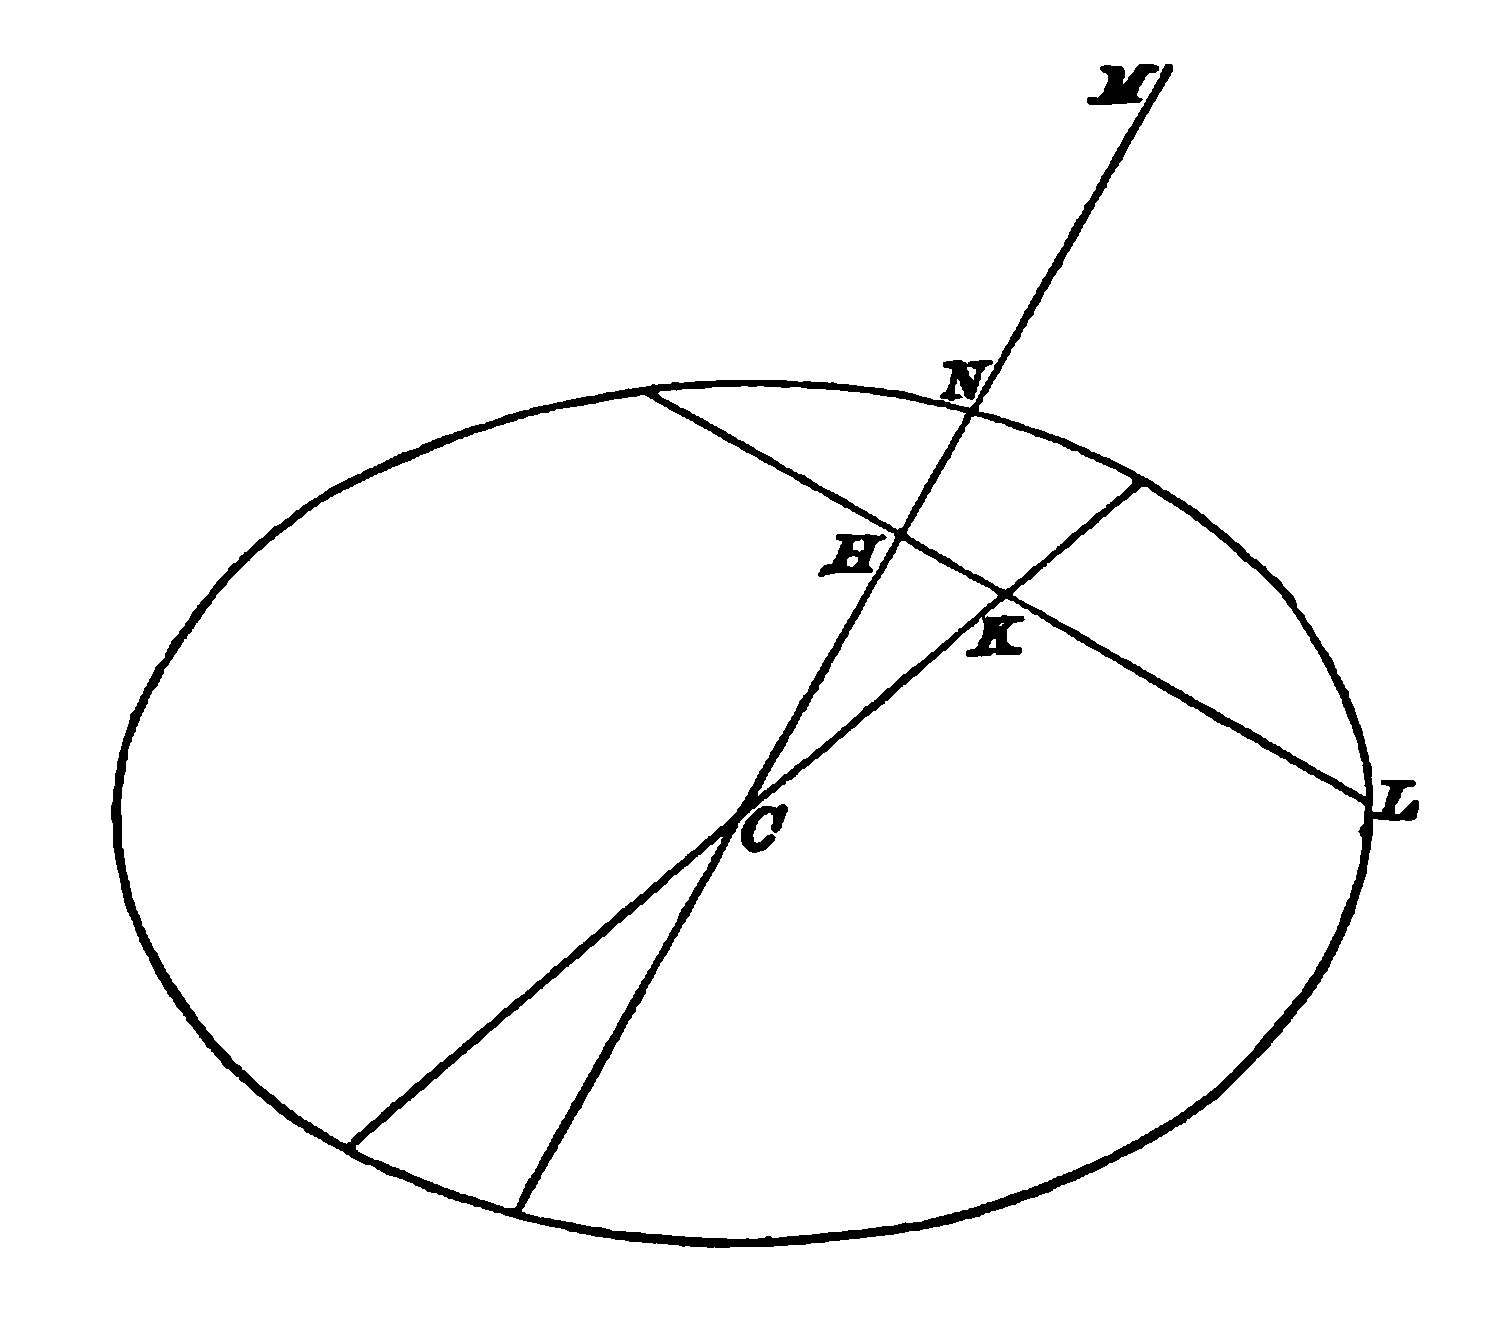
\includegraphics[width=0.6\textwidth]{243.png}
\centering
\end{figure}

Hence by Art.\ 320 we have for the attraction of the whole
oblatum at \(M\) in the direction at right angles to \(MC\) and towards
\(CK\),
\[\pi \rho \tan \beta \int_{-c}^c {\frac{x(c^2-x^2)dx}{\left\{(\gamma-x)^2+c^2-x^2\right\}^{\frac{3}{2}}}}.\]

The value of the definite integral which occurs here is \(\xp\dfrac{4c^5}{5\gamma^4}\);
Clairaut himself obtains it by a peculiar artifice. By modern
methods we may proceed thus:

Put \(\gamma^2+c^2-2\gamma x = z^2\), and let \(a=\gamma-c\), and \(b=\gamma+c\); then
we find that
\[\int_{-c}^c \frac{x(c^2-x^2)dx}{(\gamma^2+c^2-2\gamma x)^{\frac{3}{2}}} = -\frac{1}{8\gamma^4}\int_a^b (\gamma^2+c^2-z^2)(b^2-z^2)(a^2-z^2)\frac{dz}{z^2}\]
\[=\frac{ 1}{8\gamma^4}\int_a^b{\left(1- \frac{a^2+b^2}{2z^2}\right)(b^2-z^2)(a^2-z^2)}dz.\]

Integrate by parts, observing that
\[\int {\left(1- \frac{a^2+b^2}{2z^2}\right)}dz=z+ \frac{a^2+b^2}{2z};\]
%%-----File: 244.png-----%%
thus we find that the integral
\begin{align*}
&=\frac{1}{8\gamma^4}\int_a^b\left(z+\frac{a^2+b^2}{2z}\right)(a^2+b^2-2z^2)2z\,dz\\
&=\frac{1}{8\gamma^4}\int_a^b\left\{(a^2 + b^2)^2 - 4z^2\right\}\,dz\\
&=\frac{1}{8\gamma^4}\left\{(b-a)(a^2 + b^2)^2 - \frac{4}{5} (b^5 - a^5)\right\}\\
&=\frac{c}{\gamma^4}\left\{ (\gamma^2 + c^2)^2 - \frac{1}{5} (5 \gamma^4 + 10 \gamma^2 c^2 + c^4) \right\}\\
&=\frac{4c^5}{5\gamma^4}\text{.}
\end{align*}

Thus the required attraction is \(\xp\dfrac{4 \pi \rho \tan \beta c^5}{5 \gamma^4}\). The angle \(\beta\) is
exactly the same as the angle between the diameter \(CK\) and the
normal at its extremity, and is therefore very approximately equal
to the angle between \(CN\) and the normal at \(N\).

\Section
322. Clairaut introduces and defines the term \textit{ellipticity} of a
\textit{spheroid} on his page 209; with him it denotes the ratio of the
difference of the equatorial and polar diameters to the polar
diameter: so that taking \(2a\) for the equatorial diameter and \(2b\) for
the polar diameter the ellipticity is \(\xp\dfrac{a-b}{b}\). To the order however
which is sufficient for our subject we might also define the ellipticity
as \(\xp\dfrac{a-b}{a}\), and this is the sense in which we prefer to use
the term.

\Section
323. We can now give an outline of Clairaut's investigations;
we shall however change his notation for a more modern one.

Suppose the central part of the Earth solid, consisting of strata
nearly spherical; and outside this let there be homogeneous fluid.
Let \(r\) denote strictly the polar semiaxis of a stratum, but with
sufficient approximation in many cases the radius drawn from the
centre in any direction to the stratum. Let \(\rho\) denote the density
and \(\epsilon\) the ellipticity of this stratum; let \(\epsilon'\) denote the ellipticity
%%-----File: 245.png-----%%
of the stratum which forms the boundary of the solid part. Let
\(\rho_1\) denote the density of the fluid, and \(\epsilon_1\) the ellipticity of the surface
of the fluid. Let \(r'\) be the value of \(r\) at the boundary of the
solid part, and \(r_1\) the value of \(r\) at the surface of the fluid. Let \(\phi_1\)
be the angle at the point corresponding to \(r_1\) between the normal
to the stratum and \(r_1\). Thus the subscript \(1\) always indicates a
value relative to the surface of the fluid.

Since the fluid is homogeneous Huygens's principle furnishes
us with the necessary and sufficient condition for equilibrium. At
any point of the surface of the fluid we have a central force which
we will call \(F\), and a force in the meridian plane at right angles
to the radius vector towards the equator which we will call \(T\);
there is also the centrifugal force which at the equator would be
\(jF\) in our usual notation, and which will be \(jF \sin \lambda\) at the place
considered, if \(\lambda\) denote the angle between the radius vector and
the polar semiaxis. Hence resolving all the forces along the tangent
to the meridian we have as the condition of equilibrium
\[F \sin \phi_1 - T - jF \sin \lambda \cos \lambda = 0. \tag{1}\]

We must now develope this equation. With regard to \(F\) it
will be sufficient to consider the whole mass as made up of spherical
strata of varying density; and thus
\[F = \frac{4 \pi}{{r_1}^2} \int_0^{r_1} \rho r^2 dr.\]

Next consider \(T\). If there were a \textit{homogeneous} oblatum of
density \(\rho\) this force, by Art.\ 321, would be \(\xp\dfrac{4 \pi \rho \tan \beta r^5}{ 5{r_1}^4}\), where \(r\)
denotes the radius vector of the oblatum in the direction of \(r_1\).
For such an oblatum in which the radius vector is \(r + dr\) the force
would be \(\xxp\dfrac{4\pi\rho}{5{r_1}^4}\left\{ \tan \beta r^5 +\dfrac{ d}{dr} (\tan \beta r^5) dr \right\}\). Hence the force arising
from a shell of which \(\rho\) is the density and \(dr\) the thickness in the
direction of \(r_1\) is \(\xp\dfrac{4\pi\rho}{5{r_1}^4}\dfrac{d}{dr} ( \tan \beta r^5 ) dr\).

Thus we obtain
\[T = \frac{4\pi}{5{r_1}^4} \int_0^{r_1}\rho \frac{d}{dr} (\tan \beta r^5 ) dr,\]
%%-----File: 246.png-----%%
where \(\rho\), now supposed variable, indicates the density of the stratum
corresponding to \(r\).

This method of treating strata of varying density occurs very
frequently in our subject and should be carefully noticed.

Now by the nature of an ellipse it follows that to the order of
approximation which we here retain \(\tan \beta\) or \(\sin \beta\) is equal to
\(2 \epsilon \sin \lambda \cos \lambda\); and to that order \(\phi_1\) has the same meaning as \(\beta_1\).
Hence by simplifying we get from (1)
\[(2 \epsilon_1 - j) \int_0^{r_1} \rho r^2dr = \frac{2}{5{r_1}^2} \int_0^{r_1} \rho \frac{d}{dr} (\epsilon r^5) dr\tag{2}.\]

The form of (2) may be modified by separating the integral
into two parts, one extending from 0 to \(r'\), and the other from \(r'\)
to \(r_1\); in the second interval the density is constant and is denoted
by \(\rho_1\). Thus
\[\int_0^{r_1} \rho r^2dr = \int_0^{r'} \rho r^2dr + \frac{\rho_1 ({r_1}^3 - r'^{3})}{3}\text{,}\]
\[\int_0^{r_1} \rho \frac{d}{dr} (\epsilon r^5) dr = \int_0^{r'} \rho \frac{d}{dr} (\epsilon r^5) dr + \rho_1 (\epsilon_1 {r_1}^{5} - \epsilon' r'^5)\text{.}\]

If we employ the second of these modifications, (2) becomes
\[2 \epsilon_1 \left\{ \int_0^{r_1} \rho r^2dr - \frac{\rho_1 {r_1}^{3}}{5}\right\} = j \int_0^{r_1} \rho r^2dr + \frac{2}{5{r_1}^{2}} \int_0^{r'} \rho \frac{d}{dr} (\epsilon r^5) dr - \frac{2\rho_1 \epsilon' r'^{5}}{5{r_1}^{2}}\text{.}\]

If we put \(A\) for \(\displaystyle\int_0^{r'} \rho r^2dr\), and \(D\) for \(\displaystyle\int_0^{r'} \rho \xp\dfrac{d}{dr} (\epsilon r^5) dr\) we get, by
employing also the first modification,
\[\epsilon_1 = \frac{\dfrac{1}{{r_1}^{2}} (6D - 6\rho_1 \epsilon' r'^{5}) + j(15A + 5\rho_1 {r_1}^{3} - 5\rho_1 r'^{3})}{30A + 4\rho_1 {r_1}^{3} - 10\rho_1 r'^{3}}\tag{3}.\]

This is a very important formula in our subject; it agrees
with that given by Clairaut on his page 217, allowing for a misprint
with him: the investigation is substantially like his though
in form rather different.

\Section
324. The general result (3) of the preceding Article is applied
by Clairaut on his pages 218\dots 222 to some special cases.
%%-----File: 247.png-----%%

I\@. Suppose the whole mass homogeneous; then
\[A=\frac{\rho_1r'^3}{3},\quad D=\rho_1\epsilon'r'^5;\]
and we obtain
\[\epsilon_1 = \frac{5j}{4}\text{:}\]
this as far as it goes agrees with Art.\ 318.

II\@. Suppose the solid part homogeneous as well as the fluid
part, but the densities of the two parts different. Let the density
of the solid part be denoted by \(\rho_1(1+\kappa)\); then
\[A= \frac{\rho_1r'^3}{3} (1+\kappa),\quad D=\rho_1\epsilon'r'^5(1+\kappa);\]
and we obtain
\[\epsilon_1=\frac{\dfrac{6\kappa\epsilon'r'^5}{{r_1}^2} + 5j(\kappa r'^3+{r_1}^3)}{10\kappa r'^3+4{r_1}^3}.\]
We shall find hereafter that this result reappears in the \textit{Mécanique
Céleste}, Vol.\ \textsc{v}.\ page 30.

Clairaut remarks that if we consider \(\epsilon_1\) to be known by observation,
this formula will guide us in making suitable hypotheses
as to the radius, the ellipticity, and the density of the assumed
solid central part. He warns us that if we suppose \(\kappa\) to be
negative we must remember that it is to be numerically \textit{less than
unity}; but the result shews us that this is an inadequate restriction:
for if \(\kappa\) be negative it must not be numerically nearly equal
to \(\xp\dfrac{4{r_1}^3}{10r'^3}\), and this might be much less than unity if \(r'\) were nearly
equal to \(r_1\). The truth is that if \(\kappa\) be \textit{positive} the above result
may be accepted without scruple; but if \(\kappa\) be negative we must
carefully examine whether the value of \(\epsilon_1\) obtained from the
formula is a small quantity.

If in the above formula for \(\epsilon_1\) we suppose \(\epsilon' = 0\), and \(\kappa\) negative,
and put \(\xp\dfrac{\kappa r'^3}{{r_1}^3}=-\lambda\), the result agrees with that obtained on page 156.

III\@. Suppose as a particular case of II. that the solid part is to
be \textit{similar} to the whole mass, and that we require the ellipticity
%%-----File: 248.png-----%%
to be greater than it is when the whole mass is homogeneous.
Then put \({\epsilon_1 = \epsilon' = \xp\dfrac{5 j}{4}(1+p)}\), where \(p\) is some positive quantity;
thus we deduce
\[\kappa = - \frac{p {r_1}^3}{\dfrac{3}{2}\left(r'^3 - \dfrac{r'^5}{{r_1}^2}\right) + p \left(\dfrac{5}{2} r'^3 - \dfrac{3}{2} \dfrac{r^5}{{r_1}^2}\right)},\]
so that \(\kappa\) is necessarily negative.

IV\@. In the preceding result, suppose that the difference
between \(r'\) and \(r_1\) is infinitesimal; put \(r' = r_1 (1 - \lambda)\), where \(\lambda\) is
infinitesimal: then
\[\kappa = -\frac{ p}{3 \lambda + p} ,\]
so that \(\kappa\) differs only infinitesimally from unity. Thus we have
the case of a film of fluid which surrounds a solid body of infinitesimal
density; the outer and inner surfaces of the film are
similar, similarly situated, and concentric oblata.

V. Instead of being a film as in IV. let us suppose the planet
to be a shell of finite thickness; and let the internal part, though
hard, be supposed of no density or of no attracting power: then we
must solve the equation
\[\frac{3}{2}\left(r'^3 - \frac{r'^5}{{r_1}^2}\right) + p \left(\frac{5}{2} r'^3 - \frac{3}{2} \frac{r'^5}{{r_1}^2}\right) = - p {r_1}^3,\]
and take for \(\xp\dfrac{r'}{r_1}\) a positive value less than unity, if such a value
should occur among the roots of the equation.

VI\@. Now return to the suppositions in II\@. If the density of
the central part is to be greater than the density of the fluid,
and \(\epsilon_1\) to be greater than \(\xp\dfrac{5j}{4}\), then \(\epsilon'\) must be greater than \(\xp\dfrac{{r_1}^2 \epsilon_1 }{ r'^2}\).

For put \(\epsilon' = (\epsilon_1 + \gamma) \xp\dfrac{{r_1}^2}{r'^2}\), and substitute in the result given in
II.; thus we get
\[\epsilon_1 = \frac{5j}{4} + \frac{3\gamma\kappa r'^3}{2 \kappa r'^3 + 2 {r_1}^3} ;\]
and the second term will not be positive unless \(\gamma\) is positive.
%%-----File: 249.png-----%%

\Section
325. Clairaut applies the last result of the preceding Article
to two criticisms on Newton.

In the case of the Earth, if we wish to have \(\epsilon_1\) greater than
\(\xp\dfrac{5j}{4}\), it is \textit{not sufficient} merely to suppose a solid nucleus of greater
density than the fluid; it is necessary to have the ellipticity of this
solid nucleus greater than \(\xp\dfrac{{r_1}^2 \epsilon_1}{r'^2}\): see Art.\ 37.

In the case of Jupiter, if we wish to have \(\epsilon_1\) less than \(\xp\dfrac{5j}{4}\), it is
\textit{not necessary} to suppose that the equatorial parts have been
scorched by the Sun into a greater density than the other parts;
it is sufficient to suppose that the solid nucleus is denser than the
fluid, and that it has an ellipticity less than \(\xp\dfrac{{r_1}^2 \epsilon_1 }{r'^2}\): see Art.\ 31.

\Section
326. Clairaut shews in his pages 224 and 225, that an
oblongum may be a form of relative equilibrium.

For in case II. of Art.\ 324, if \(\epsilon'\) is negative and numerically
greater than \(\xp\dfrac{5j(\kappa r'^3 + {r_1}^3) {r_1}^2 }{6\kappa r'^5}\), then \(\epsilon_1\) is negative.

But even if \(\epsilon'\) is positive, it will be possible to have \(\epsilon_1\) negative
if \(\kappa\) be negative; Clairaut does not make this remark, to which
D'Alembert seems to attach great importance; see the \textit{Opuscules
Mathématiques}, Vol.\ \textsc{vi}.\ page 77. The fact simply is that Clairaut's
general formula contains somewhat more than he himself verbally
drew from it.

\Section
327. Suppose the depth of the sea to be not greater than the
height of the mountains; then Clairaut considers that we may
without sensible error regard the earth as an oblatum covered
with a film of water; see his page 225. In this case he takes
\(\epsilon_1 = \epsilon'\), and \(r_1 = r'\); and so the equation (3) of Art.\ 323 becomes
\[10A \epsilon_1 -\frac{ 2D}{{r_1}^2} = 5Aj.\]
%%-----File: 250.png-----%%

\Section
328. It had been objected that Clairaut ought not to have
supposed \(\epsilon_1 = \epsilon'\): see D'Alembert's \textit{Opuscules Mathématiques} Vol \textsc{vi}.\
page 75, and Cousin's \textit{Astronomie Physique}, page 164. If then we
put \(r_1 = r'\), but do not put \(\epsilon_1 = \epsilon'\), the equation (3) of Art.\ 323
becomes
\[(10A - 2\rho_1 {r_1}^{3}) \epsilon_1 = \frac{2}{{r_1}^{2}} (D - \rho_1\epsilon'{r_1}^{5}) + 5Aj\text{.}\]

As before then we may say that Clairaut's general formula
contains more than he was contented to draw from it. But we
must observe that if we suppose the stratum of fluid to be very
thin, but do not take \(\epsilon_1 = \epsilon'\), the fluid will not necessarily \textit{cover} all
the solid: either the polar parts or the equatorial parts may be
left without fluid.

\Section
329. Clairaut applies his result which we have given in
Art.\ 327 to shew that if \(\epsilon = \epsilon_1 \xp\left(\dfrac{{r_1}^{2}}{r^2} - u\right)\), where \(u\) is positive, and
the density diminishes continually from the centre, the ellipticity
will be less than when the mass is homogeneous.

For, using this expression for \(\epsilon\), we have
\begin{gather*}
D = \int_{0}^{r_{1}} \rho \frac{d}{dr} (\epsilon r^5) dr = 3\epsilon_1 {r_1}^{2} \int_{0}^{r_{1}} \rho r^2 dr - \epsilon_1 \int_{0}^{r_{1}} \rho \frac{d}{dr} (r^5 u) dr\\
\begin{aligned}&= 3\epsilon_1 {r_1}^{2} A - \epsilon_1 (\rho r^5 u)_1 + \epsilon_1 \int_{0}^{r_{1}} r^5 u \frac{d\rho}{dr} dr\\
&= 3\epsilon_1 {r_1}^{2} A - \epsilon_1 G\text{ say,}
\end{aligned}
\end{gather*}
where \(G\) is some positive quantity, since by supposition \(\xp\dfrac{d\rho}{dr}\) is
negative.

Thus we obtain,
\[10A\epsilon_1 - 6A\epsilon_1 + \frac{2}{{r_1}^{2}} \epsilon_1 G = 5Aj\text{,}\]
so that
\[\epsilon_1 = \frac{5j}{4} \frac{1}{1 + \dfrac{G}{2{r_1}^{2} A}}\text{,}\]
which is less than \(\xp\dfrac{5j}{4}\).
%%-----File: 251.png-----%%

Clairaut expresses his result very awkwardly in words; he says
that the spheroid will be less flattened than in the homogeneous
case, unless the ellipticity of the strata diminishes from the centre
to the circumference, and in a \textit{greater ratio than the squares of the
distances}. The language would imply that the squares of the
distances diminish from the centre to the circumference. He
should have said, \textit{provided the product of the ellipticity into the
square of the distance is never greater than at the surface}.

Clairaut on his pages 228\dots 232 gives some special cases of the
general result in Art.\ 328, by assuming special laws of density;
his results are accurate, and he points out the objection to some
corresponding investigations of Maclaurin: see Art.\ 267.

\Section
330. Clairaut's third Chapter occupies pages 233\dots 262; it
discusses the law of the variation of gravity at the surface of a
spheroid of revolution composed of strata of varying density and
ellipticity. Clairaut shews that the diminution of gravity in
passing from the pole to the equator varies as the square of the
cosine of the latitude; and he establishes the theorem which we
now call \textit{Clairaut's Theorem}. We will proceed to give some details.

\Section
331. Suppose a particle placed outside a circular lamina;
when the projection of the particle on the lamina is very near the
centre of the circle, the resultant attraction on the particle is very
nearly the same as if the particle were at the same distance from
the centre of the circle, but had its projection coincident with the
centre: Clairaut shews this briefly by general reasoning. If we
proceed analytically as in Art.\ 320, we shall find that when the
particle is displaced so that its projection moves from the centre to
a distance \(h\) from the centre, the attraction \textit{perpendicular} to the
lamina is not changed to the order \(h\), while there is a \textit{transverse}
attraction produced of the order \(h\); so that the change in the
resultant attraction is of the order \(h^2\).

The result holds also for an ellipse or any other central curve.

\Section
332. If a circular lamina, and an oval lamina which is nearly
circular, have the same centre and the same plane and equal areas,
they exert approximately the same attraction on a particle, the
%%-----File: 252.png-----%%
projection of which would coincide with the common centre:
Clairaut shews this briefly by general reasoning.

\Section
333. The propositions of the two preceding Articles lead
Clairaut to the following general result.

Let \(C\) be the centre of an ellipsoid of revolution nearly
spherical, and \(M\) an external particle; let \(MC\) cut the solid at \(N\),
and let \(MC\) produced cut the solid at \(n\); the attraction of the solid
on a particle at \(M\) is approximately the same as that of an
ellipsoid of revolution of equal volume having \(Nn\) for its axis of
revolution.

The original solid may be an oblatum or an oblongum; whichever
it be the derived solid will be sometimes an oblatum and
sometimes an oblongum, according to the position of the straight
line \(CM\).

It must be observed that the approximation holds as far as
the first power of the ellipticity \textit{inclusive}; in fact the errors in
Arts.\ 331 and 332 are of the order of the \textit{square} of the ellipticity.

\Section
334. Clairaut then finds the attraction of an ellipsoid of
revolution which is nearly spherical on a particle which is on the
prolongation of the axis of revolution. I have already adverted to
the method which he uses: see Art.\ 165. The result is correct to
the first power of the ellipticity inclusive.

\Section
335. The pages 233\dots 243 of Clairaut's work which we have
just considered were, in substance, originally published in the
\textit{Philosophical Transactions}; see Art.\ 164: these pages well deserve
perusal as a good specimen of the ingenuity and simplicity of
Clairaut's investigations.

A modern student will probably like to verify by analysis the
important result in Art.\ 333. The simplest way perhaps is to find
the \textit{potential} of the original ellipsoid of revolution on the particle
at \(M\), and shew that it is equal to the potential of the derived
ellipsoid of revolution, so far as terms of the first order inclusive.

Take \(C\) for the origin, \(CN\) for the axis of \(z\); let the axis of \(y\) be
the diameter which is conjugate to \(Nn\) in the meridian plane of
%%-----File: 253.png-----%%
the given ellipsoid which contains \(CM\); let the axis of \(x\) be at right
angles to those of \(y\) and \(z\).

Let \(CM = \gamma\); let \(\chi\) denote the angle between the axes of \(y\)
and \(z\). Then the potential of the given ellipsoid is
\[\iiint \frac{\sin \chi dx dy dz}{\{x^2 + y^2 + 2y(z - \gamma) \cos \chi + (z - \gamma)^2\}^{\frac{1}{2}}}\text{;}\]
the limits of the integration are determined by the equation to the
given ellipsoid, which we may take as
\[\frac{x^2}{a^2} + \frac{y^2}{b^2} + \frac{z^2}{c^2} = 1\text{.}\]

Put \(r^2\) for \(x^2 +y^2 + (z - \gamma)^2\); then we may expand the term
under the integral signs in the form
\[\frac{1}{r} - \frac{y (z-\gamma) \cos \chi}{r^3} + \frac{3}{2} \frac{y^2 (z-\gamma)^2 \cos^2 \chi}{r^5} + \ldots\]

The second of these terms gives zero as the result when integrated,
because \(y\) is as often negative as positive. Thus if we
reject the \textit{squares} and the higher powers of the small quantity
\(\cos \chi\), the potential becomes
\[\sin \chi \iiint \frac{dx dy dz}{\{x^2 + y^2 + (z- \gamma)^2\}^{\frac{1}{2}}}\text{.}\]

Assume \(x = a \xi\), \(y = b \eta\), \(z = c \zeta\); then the potential can be
transformed to
\[V \iiint \frac{d\xi d\eta d\zeta}{\{a^2 \xi^2 + b^2 \eta^2 + (c \zeta - \gamma)^2\}^{\frac{1}{2}}}\tag{1},\]
where \(V\) stands for \(abc \sin \chi\), and the limits of integration are
determined by
\[\xi^2 + \eta^2 + \zeta^2 = 1\text{.}\]

Now when we form the potential of the derived ellipsoid we
obtain, if \(h\) denote the two equal semiaxes,
\[h^2 c \iiint \frac{d\xi d\eta d\zeta}{\{h^2 \xi^2 + h^2 \eta^2 + (c \zeta - \gamma)^2\}^{\frac{1}{2}}}\tag{2},\]
%%-----File: 254.png-----%%
the limits being the same as before. And by the condition of
equal volumes we have
\[abc \sin \chi = h^2 c\tag{3}.\]

Since the original ellipsoid is nearly spherical we have
\[a = c(1 + \lambda)\quad\text{and}\quad b = c(1 + \mu)\]
where \(\lambda\) and \(\mu\) are small, being of the order of the ellipticities.

Thus from (3) we have
\[h^2 = c^2(1 + \lambda + \mu) \sin \chi\text{,}\]
but \(\sin \chi\) being the sine of an angle, nearly a right angle, we shall
find that it differs from unity by a quantity which is of the order
of the \textit{squares} of the ellipticities. Thus to our order
\[h^2 = c^2 (1 + \lambda + \mu)\text{,}\]
and so we have to our order
\[h^2 = \frac{a^2 + b^2}{2}\text{.}\]

Hence since \(a^2 = \xp\dfrac{a^2 + b^2}{2} + \xp\dfrac{a^2 - b^2}{2}\), and \(b^2 = \xp\dfrac{a^2 + b^2}{2} - \xp\dfrac{a^2 - b^2}{2}\),
we see that to our order (1) becomes
\[V \iiint \frac{d\xi d\eta d\zeta}{\left\{h^2 \xi^2 + h^2 \eta^2 + \dfrac{a^2 - b^2}{2} (\xi^2 - \eta^2) + (c \zeta - \gamma)^2\right\}^{\frac{1}{2}}}\text{.}\]

Expand the denominator under the integral sign in powers of
\(\xp\dfrac{a^2 - b^2}{2} (\xi^2 - \eta^2)\); then the term under the integral sign which
involves the first power of this small quantity obviously vanishes
by symmetry: so if we neglect the square of \(a^2 - b^2\), the expression
(1) reduces to the form (2). This is the required result.

\Section
336. We are now prepared to find the value of gravity at any
point of the surface of our hypothetical Earth.

Suppose \(r\) the polar radius, \(r (1 + \epsilon)\) the equatorial radius of
an oblatum, where \(\epsilon\) is small; let \(\rho\) be the density. We shall
first determine the attraction on a particle at the distance \(R\) from
the centre, the direction of \(R\) making with the polar axis an angle
whose sine is \(s\).
%%-----File: 255.png-----%%

By Clairaut's proposition in Art.\ 333, we substitute instead of
the oblatum, a certain ellipsoid of revolution of equal mass. Let
\(c\) denote the polar semiaxis, and \(\lambda\) the ellipticity of this derived
ellipsoid. The attraction which it exerts
\[= \frac{\text{mass of oblatum}}{R^2} \left(1 - \frac{6\lambda c^2}{5R^2}\right)\text{:}\]
this may be deduced from Art.\ 261, supposing \(\lambda\) positive; or it
may be obtained in Clairaut's manner, to which we have referred
in Art.\ 334, and then it will be found to hold whether \(\lambda\) be positive
or negative.

Now to our order of approximation
\[c = r(1 + \epsilon s^2)\text{;}\]
and the condition of equal masses gives
\[r^3 (1 + 2 \epsilon) = c^3 (1 + 2 \lambda) = r^3 (1 + 3 \epsilon s^2)(1 + 2 \lambda)\text{;}\]
so that
\[\lambda = \left(1 - \frac{3s^2}{2}\right) \epsilon\text{.}\]

Also, supposing the attracted particle to be on a concentric and
similarly situated oblatum, the dimensions of which are given by
\(r_1\) and \(\epsilon_1\), we have
\[R = r_1 (1 + \epsilon_1 s^2)\text{.}\]

The mass of the oblatum \(= \xp\dfrac{4 \pi r^3}{3} (1 + 2 \epsilon) \rho\).

Hence the attraction of the oblatum
\begin{align*}
&= \frac{4 \pi r^3}{3{r_1}^{2}} (1 + 2 \epsilon)(1 - 2 \epsilon_1 s^2) \rho \left\{1 - \frac{6r^2}{5{r_1}^{2}} (1 - \frac{3}{2} s^2) \epsilon\right\}\\
&= \frac{4 \pi r^3 \rho}{3{r_1}^{2}} \left\{1 + 2 \epsilon - 2 \epsilon_1 s^2 - \frac{6 \epsilon r^2}{5{r_1}^{2}} + \frac{9 \epsilon s^2 r^2}{5{r_1}^{2}}\right\}\text{.}
\end{align*}

Let us denote this for a moment by \(\rho f(r)\); then for the
attraction of the shell of density \(\rho\), comprised between the surfaces
which correspond to \(r\) and \(r + dr\), we have \(\rho \xp\dfrac{df(r)}{dr} dr\).
%%-----File: 256.png-----%%

Hence, if we suppose the density of each shell to be uniform,
but the density to vary from shell to shell, we have for the whole
attraction
\[\int_{0}^{r_{1}} \rho \frac{df(r)}{dr} dr\text{.}\]

Let \(A = \displaystyle\int_{0}^{r_{1}} \rho r^2 dr\),\quad \(B = \displaystyle\int_{0}^{r_{1}} \rho \frac{d(r^3 \epsilon)}{dr} dr\),\quad \(D = \displaystyle\int_{0}^{r_{1}} \rho \frac{d(r^5 \epsilon)}{dr} dr\), then
the attraction is
\[\frac{4\pi}{{r_1}^{2}} (1 - 2\epsilon_1 s^2) A + \frac{8\pi B}{3{r_1}^{2}} - \frac{4\pi}{5{r_1}^{4}} (2 - 3s^2)D\text{.}\]

We must now introduce the centrifugal force. The centrifugal
force at the equator is approximately \(\xp\dfrac{4\pi jA}{{r_1}^{2}}\); and therefore
it is \(\xp\dfrac{4\pi sjA}{{r_1}^{2}}\) at the point under consideration: the resolved part
of this along the radius is \(\xp\dfrac{4\pi s^2 jA}{{r_1}^{2}}\), which must be subtracted from
the \textit{attraction} to obtain the \textit{gravity}.

Hence the gravity at the point under consideration
\[= \frac{4\pi}{{r_1}^{2}} (1 - 2\epsilon_1 s^2) A + \frac{8\pi B}{3{r_1}^{2}} - \frac{4\pi}{5{r_1}^{4}} (2 - 3s^2) D - \frac{4\pi s^2 jA}{{r_1}^{2}}\text{.}\]

Let \(P\) denote the gravity at the pole, \(g\) the gravity at the
point under consideration; then
\[P - g = \frac{4\pi}{{r_1}^{2}} \left\{(j + 2\epsilon_1) A - \frac{3D}{5{r_1}^{2}}\right\} s^2\text{.}\]

Thus \(P - g\) varies as \(s^2\); that is, the diminution of gravity in
passing from the pole to the equator varies as the square of the
cosine of the latitude.

Let \(E\) denote the gravity at the equator; then
\[P - E = \frac{4\pi}{{r_1}^{2}}\left\{(j + 2\epsilon_1) A - \frac{3D}{5{r_1}^{2}}\right\}\text{.}\]

Divide this by \(E\); then on the right-hand side it will be
sufficient to use \(\xp\dfrac{4\pi A}{{r_1}^{2}}\) for \(E\), so that
\[\frac{P - E}{E} = j + 2\epsilon_1 - \frac{3D}{5A{r_1}^{2}}\text{.}\]
%%-----File: 257.png-----%%

Substitute for \(\xp\dfrac{D}{A}\) from Art.\ 327, and we have
\[\frac{P - E}{E} = \frac{5}{2}j - \epsilon_1\text{.}\]

This remarkable result is called \textit{Clairaut's Theorem}. The fraction
\(\xp\dfrac{P - E}{E}\) we shall call \textit{Clairaut's fraction}, as in Art.\ 171, and
shall denote it by \(v\); so that we have
\[v + \epsilon_1 = \frac{5}{2}j\text{.}\]

We know by Art.\ 28 that \(\xp\dfrac{5}{2}j\) is twice the ellipticity of the
earth, supposed homogeneous; and this is the form in which
Clairaut himself expresses this term.

\Section
337. The assumptions on which Clairaut's demonstration of
his famous theorem rests should be carefully noticed. The strata
are supposed to be ellipsoidal, and of revolution round a common
axis, and nearly spherical. Each stratum is homogeneous, but
there is no limitation on the law by which the density varies from
stratum to stratum: the density may change discontinuously if
we please. It is not assumed that the strata were originally fluid;
but it is assumed that the \textit{superficial} stratum has the same form
as if it were fluid and in relative equilibrium when rotating with
uniform angular velocity. There is no limitation on the law by
which the ellipticity varies from stratum to stratum, except that
the ellipticity must be continuous, and at the surface must be
such as would correspond to the relative equilibrium of a film
of rotating fluid.

We shall find that D'Alembert in 1756 mistook the range of
Clairaut's demonstration: see the \textit{Recherches sur \dots\ Systême du
Monde}, Vol.\ \textsc{iii}.\ page 187.

In some modern works there has been a want of strict accuracy
as to the Theorem, owing perhaps to an undue regard to
brevity. Thus we read in one that Clairaut established his
Theorem on ``the hypothesis of the Earth being a fluid mass'';
and we read in another that Clairaut discovered his Theorem for
``the case of a rotating fluid mass, or solid with density distributed
as if fluid.''
%%-----File: 258.png-----%%

\Section
338. Clairaut on his pages 251\dots 259 uses his theorem to support
certain criticisms on Newton, David Gregory, and Maclaurin.
We have already noticed these criticisms: see Arts.\ 30, 84, and 271.

On his pages 260\dots 262 Clairaut in like manner uses his
theorem in relation to Cassini's hypothesis that the earth was an
oblongum with an ellipticity of \(\xp\dfrac{1}{93}\). In Art.\ 336 put \(\epsilon_{1} = -\xp\dfrac{1}{93}\),
and \(j = \xp\dfrac{1}{289}\); then we get approximately \(v = \xp\dfrac{1}{93} + \xp\dfrac{1}{115} = \xp\dfrac{1}{51}\).
But, as Clairaut observes, this is a far greater value of \(v\) than
pendulum observations warrant. Cassini's number however seems
to have been 95 not 93: see Art.\ 104.

\Section
339. Clairaut's fourth Chapter occupies pages 262\dots 296; it
considers the figure of the Earth, supposed to have been originally
fluid, and composed of strata of varying densities. In fact Clairaut
now proposes to investigate the connection between the density
and the ellipticity in order that strata of the kind considered in
the preceding Chapter may be in relative equilibrium if they are
fluid. A process like that of Art.\ 323 must now be applied to
\textit{each} stratum.

\Section
340. Suppose a shell of density \(\rho\) bounded by two concentric
and similarly situated oblata; let \(\zeta_{1}\) be the ellipticity of the inner
surface, and \(\zeta_{2}\) the ellipticity of the outer surface. Suppose a
particle situated on the inner surface of the shell; we shall determine
the attraction which the shell exerts on this particle in the
direction at right angles to the radius vector from the centre of
the shell to the particle. This problem is solved by Clairaut on
his pages 262\dots 265. Our solution is substantially the same.

The attraction of the shell is of course equal to the difference
of the attractions of the oblatum which is bounded by the outer
surface, and the oblatum which is bounded by the inner surface.
We will consider these bodies separately, beginning with the larger.

The larger oblatum produces the same effect as would be produced
by a similar, similarly situated, and concentric oblatum,
having the particle on its surface; for the difference of these two
similar, similarly situated, and concentric oblata produces no effect
by Art.\ 13.
%%-----File: 259.png-----%%

Hence the attraction of the larger oblatum in the assigned
direction is \(\xp\dfrac{4\pi\rho c \tan \beta}{5}\) in the notation of Art.\ 321; for now \(\gamma = c\).
And, as in Art.\ 323, we have \(\tan \beta = 2\zeta_{2} \sin \lambda \cos \lambda\), so that the
attraction becomes \(\xp\dfrac{8\pi\rho c\zeta_{2} \sin \lambda \cos \lambda}{5}\).

In like manner the attraction of the smaller oblatum in the
assigned direction is \(\xp\dfrac{8\pi\rho c\zeta_{1} \sin \lambda \cos \lambda}{5}\).

Thus it follows that the required attraction of the shell in the
assigned direction is \(\xp\dfrac{8\pi\rho c (\zeta_{2} - \zeta_{1}) \sin \lambda \cos \lambda}{5}\).

Now suppose that there is an infinitesimally thin shell of the
density \(\rho\); let \(r\) be the polar semiaxis of the inner surface, and \(\epsilon\)
the ellipticity of this surface; then \(\epsilon + \xp\dfrac{d\epsilon}{dr}dr\) will denote the ellipticity
of the outer surface. Therefore the attraction, in the direction
at right angles to the radius vector, of this shell on the inside
particle is \(\xp\dfrac{8\pi\rho}{5}c \sin \lambda \cos \lambda \xp\dfrac{d\epsilon}{dr}dr\); this is obvious from the preceding
investigation.

\Section
341. We now proceed to apply a process like that of Art.\ 323
to any stratum.

Let there be a particle of fluid in any stratum at the distance
\(r'\) from the centre; let \(\lambda\) be the angle between the radius vector
to the particle and the polar semiaxis.

The central attraction on the particle is \(\xp\dfrac{4\pi}{r'^{2}} \displaystyle\int_0^{r'} \rho r^2 dr\), approximately;
for the strata beyond the particle produce no central effect
to the order of accuracy which we have to consider. This central
attraction gives rise to a component in the meridian plane, at
right angles to the radius vector, towards the pole equal to
\(2\epsilon' \sin \lambda \cos \lambda \times \xp\dfrac{4\pi}{r'^{2}} \displaystyle\int_0^{r'} \rho r^2 dr\). We will call this a \textit{transverse} attraction.
%%-----File: 260.png-----%%

The transverse attraction on the particle from the strata below
the particle towards the equator, is \(\xp\dfrac{8\pi r' \sin \lambda \cos \lambda}{5r'^{5}} \displaystyle\int_0^{r'} \rho \frac{d}{dr} (r^5\epsilon)dr\),
by Art.\ 323.

The transverse attraction on the particle from the strata beyond
the particle towards the equator is \(\xp\dfrac{8\pi r' \sin \lambda \cos \lambda}{5} \displaystyle\int_{r'}^{r_1} \rho \frac{d\epsilon}{dr} dr\),
by Art 340.

Let \(\omega\) denote the angular velocity; then the transverse component
of the centrifugal force is \(\omega^2 r' \sin \lambda \cos \lambda\).

Hence, as in Art.\ 323, equating to zero the whole transverse
force, and dividing by \(4\pi \sin \lambda \cos \lambda\) we obtain
\[\frac{2\epsilon'}{r'^{2}} \int_0^{r'} \rho r^2dr - \frac{2}{5r^4} \int_0^{r'} \rho \frac{d}{dr} (\epsilon r^5) dr - \frac{2r'}{5} \int_{r'}^{r_1} \rho \frac{d\epsilon}{dr} dr - \frac{r' \omega^2}{4\pi} = 0\text{.}\]

If as usual we denote by \(j\) the ratio of the centrifugal force at
the equator at the surface of the fluid to the attraction there, we
have to the order of accuracy which we require
\[r_1 \omega^2 = j \frac{4\pi}{{r_1}^{2}} \int_0^{r_1} \rho r^2dr\text{.}\]
Substituting this value of \(\omega^2\) our equation becomes
\[\frac{2\epsilon'}{r'^{2}} \int_0^{r'} \rho r^2dr - \frac{2}{5r'^{4}}\int_0^{r'} \rho \frac{d}{dr} (\epsilon r^5) dr - \frac{2r'}{5}\int_{r'}^{r_1} \rho \frac{d\epsilon}{dr} dr - \frac{jr'}{{r_1}^{3}}\int_0^{r_1} \rho r^2dr = 0\text{.}\]

This important equation occurs for the first time in Clairaut's
page 273; it has ever since been permanently associated with the
subject: I shall call it \textit{Clairaut's primary equation}. Whether we
leave \(\omega^2\) in the equation, or substitute for it in the manner just
explained, is of no consequence.

\Section
342. If \(\epsilon\) and \(\rho\) are taken so as to satisfy Clairaut's primary
equation we have a \textit{possible} constitution for the earth. Clairaut
however asserts more than this on his page 265, namely that if \(j\)
be very small the strata \textit{will} be elliptical spheroids. Even Laplace
has scarcely arrived at this point; he has only shewn that if the
strata \textit{are assumed} to be nearly spherical they must be elliptical
spheroids.
%%-----File: 261.png-----%%

\Section
343. Clairaut transforms his primary equation. It will not
lead to any confusion if we now drop the accent from \(r'\) and from
\(\epsilon'\): we may then write the equation thus:
\[10 \epsilon r^2 \int_0^r \rho r^2dr - 2 \int_0^r \rho \frac{d}{dr} (\epsilon r^5) dr-2r^5 \int_r^{r_1} \rho \frac{d \epsilon}{dr} dr - \frac{5r^5 \omega^2}{4 \pi} = 0\text{.}\]

Differentiate with respect to \(r\); thus
\begin{multline*}
\left(20 \epsilon r + 10r^2 \frac{d\epsilon}{dr}\right) \int_0^r \rho r^2 dr + 10 \rho r^4 \epsilon - 2 \rho \frac{d}{dr} (\epsilon r^5)\\
-10r^4 \int_r^{r_1} \rho \frac{d\epsilon}{dr} dr + 2r^5 \rho \frac{d \epsilon}{dr} - \frac{25r^4 \omega^2}{4\pi} = 0\text{.}
\end{multline*}

Simplify, and divide by \(10r^4\); thus
\[\left(\frac{1}{r^2} \frac{d \epsilon}{dr} + \frac{2 \epsilon}{r^3}\right) \int_0^r \rho r^2dr = \int_r^{r_1} \rho \frac{d \epsilon}{dr} dr + \frac{5 \omega^2}{8 \pi}\text{.}\]

Differentiate again with respect to \(r\); thus
\[\left(\frac{1}{r^2} \frac{d^2 \epsilon}{dr^3} - \frac{6 \epsilon}{r^4}\right) \int_0^r \rho r^2 dr+ \rho\left(\frac{d \epsilon}{dr} + \frac{2 \epsilon}{r}\right) = - \rho \frac{d \epsilon}{dr}\text{,}\]
so that
\[\frac{d^2\epsilon}{dr^2} + \frac{2\rho r^2 \dfrac{d \epsilon}{dr}}{\displaystyle\int_0^r \rho r^2dr} = \left( \frac{6}{r^2} - \frac{2\rho r}{\displaystyle\int_0^r \rho r^2dr}\right) \epsilon\text{.}\]
This I shall call \textit{Clairaut's derived equation}.

\Section
344. Clairaut puts his derived equation in another form.

Let \(\xp\dfrac{1}{\epsilon} \xp\dfrac{d \epsilon}{dr}\) be denoted by \(u\); so that \(\xp\dfrac{d\epsilon}{dr} =\epsilon u\).

Then
\[\frac{d^2 \epsilon}{dr^2} = \epsilon u^2 + \epsilon \frac{du}{dr}\text{.}\]

Thus
\[\frac{du}{dr} + u^2 = - \frac{2u \rho r^2}{\displaystyle\int_0^r \rho r^2dr} + \frac{6}{r^2} - \frac{2 \rho r}{\displaystyle\int_0^r \rho r^2dr}\text{.}\]
%%-----File: 262.png-----%%

Put \(u + \xp\dfrac{ \rho r^2}{\displaystyle\int_0^r{ \rho r^2} dr} = t\); and then we obtain
\[\frac{dt}{dr} + t^2 =\frac{ r^2 \dfrac{d \rho}{dr}}{\displaystyle\int_0^r {\rho r^2} dr} + \frac{6}{r^2}.\]

Clairaut observes that this equation falls under the case of
\(dy + y^n dx = X dx\), where \(X\) is a function of \(x\); and that what we
now call the separation of the variables had not yet been effected
in general. Accordingly he does not propose to seek for the
ellipticities which correspond to a given law of density, except in
the case in which \(\rho\) varies as \(r^n\). See his page 276.

\Section
345. Suppose then that \(\rho\) varies as \(r^n\). We have by the
preceding Article
\[\frac{dt}{dr} + t^2 = \frac{n^2 + 3n + 6}{r^2}\text{.}\]

This becomes homogeneous and easily integrable by putting a
new variable instead of \(\dfrac{1}{r}\); and thus we obtain
\[t = \frac{\dfrac{1}{2} + q}{r} - \frac{2qar^{-2q-1}}{ar^{-2q} + 1},\]
where \(q = \bigsurd\left(n^2 + 3n + \dfrac{25}{4}\right)\), and \(a\) is an arbitrary constant.

With this value of \(t\) we find
\[\epsilon = bar^{-n-\frac{5}{2}-q} + br^{-n-\frac{5}{2}+q},\]
where \(b\) is another arbitrary constant.

This value of \(\epsilon\) then satisfies Clairaut's derived equation; we
must examine if it also satisfies the primary equation. Substitute
the value of \(\epsilon\), and we find after simplification that the primary
equation is satisfied provided the following relation holds between
the constants:
\[\left(q -\frac{ 1}{2} - n\right)b{r_1}^{\frac{1}{2} + q} - ba\left(q + \frac{1}{2} + n\right){r_1}^{\frac{1}{2}-q} = \frac{5j}{2} {r_1}^{n+3}.\]
%%-----File: 263.png-----%%

Thus there is only one relation between two constants, and so
it would appear that the solution is not determinate. Clairaut
offers an explanation on this point. It has been assumed throughout
that the ellipticity of the strata is small; moreover he considers
that \(n\) must be negative in order that the density may diminish
from the centre to the circumference, which he says the laws of
hydrostatics require: see Art.\ 315. Hence we must have \(a = 0\);
for otherwise \(\epsilon\) would be infinite at the centre.

Also even if \(n\) be considered positive we must have \(a = 0\); in
this case \(\epsilon\) would be finite at the centre, but \(r\epsilon\) would be infinitesimal:
see Clairaut's page 281.

For a particular case suppose \(n = 0\), then \(q = \xp\dfrac{5}{2}\); and after
putting \(a = 0\) we obtain \(b = \xp\dfrac{5j}{4}\): and then \(\epsilon = b = \xp\dfrac{5j}{4}\) as it should be.

\Section
346. Clairaut's derived equation may be put in the form
\[\frac{6\epsilon - r^2 \dfrac{d^2\epsilon}{dr^2}}{2r\epsilon + 2r^2 \dfrac{d\epsilon}{dr}} = \frac{\rho r^2}{\displaystyle\int_{0}^{r} \rho r^2dr}\text{.}\]

Then if \(\epsilon\) be given as a function of \(r\), the left-hand member of
the equation becomes a known function of \(r\); denote it by \(P\);
from this we deduce \(\rho r^2 = Pe^{\int Pdr}\) which gives \(\rho\). See Clairaut's
page 283.

\Section
347. The formulæ which have been investigated for the case
of an infinite number of indefinitely thin strata may be applied to
the case of a finite number of shells surrounding a central part,
the density changing abruptly from the central part to the
adjacent shell, and then from shell to shell. Clairaut considers
this on his pages 286\dots 293; taking the density constant throughout
the central part, and throughout each shell.

He shews that the ellipticities increase from the centre to the
surface, assuming that the densities diminish from the centre to
the surface: see his page 292.
%%-----File: 264.png-----%%

Clairaut takes for an example the case in which the whole
mass is supposed to consist of two parts throughout each of which
the density is constant. Let \(\rho_1\) be the density of the outer part,
\(\epsilon_1\) the ellipticity of the outer surface, \(r_1\) the polar semiaxis; let
\(\rho_2\), \(\epsilon_2\), and \(r_2\) be corresponding quantities for the inner part. Then
in the integrations which occur in Clairaut's primary equation we
have to make \(\rho = \rho_2\) from \(r = 0\) to \(r = r_2\), and \(\rho = \rho_1\) from \(r = r_2\) to
\(r = r_1\). Put \(\lambda\) for \(\xp\dfrac{r_2}{r_1}\), and suppose \(\rho_2 = \rho_1 + \sigma\). Then apply Clairaut's
primary equation first to the extreme stratum of the inner part,
and next to the extreme stratum of the outer part: thus we obtain
after reductions
\[\epsilon_2 (10\rho_1 + 4 \sigma) - 6 \epsilon_1 \rho_1 = 5j (\rho_1 + \sigma \lambda^3)\text{,}\]
\[\epsilon_1 (4 \rho_1 + 10 \sigma \lambda^3) - 6 \epsilon_2 \sigma \lambda^5 = 5j (\rho_1 + \sigma \lambda^3)\text{.}\]

From these equations we deduce
\[\epsilon_1 (\rho_1 + \sigma \lambda^3) = \epsilon_2 \left(\rho_1 + \frac{2}{5} \sigma + \frac{3}{5} \sigma \lambda^5\right)\text{,}\]
\[\epsilon_2 = \frac{25j(\rho_1 + \sigma \lambda^3)^2}{(10\rho_1+4\sigma)(2\rho_1+5\sigma \lambda^3)-18\rho_1 \sigma \lambda^5}\text{.}\]

\Section
348. In his pages 294 and 295, Clairaut points out two limits
for the ellipticity of a planet, assuming that the planet was originally
fluid, and that the denser strata are the nearer to the centre.
One limit is the ellipticity which corresponds to the case of a
homogeneous mass. The other limit is that in which the attraction
at any point is directed towards the centre, and varies inversely as
the square of the distance from the centre, for this may be regarded
as equivalent to having the density infinite at the centre: see
Arts.\ 64 and 173.

Clairaut states on his page 296 that the theorem which we
now call \textit{Clairaut's Theorem}, holds for the case in which the earth
is supposed to have been originally a fluid of the nature which he
has considered. This is obvious from the demonstration already
given: see Art.\ 336.
%%-----File: 265.png-----%%

\Section
349. Clairaut's fifth Chapter occupies pages 296\dots 304; it is
on the comparison of the theory with observation.

Clairaut considers that the observations of the diminution of
gravity in passing from the pole to the equator agree sufficiently
well with his theory. But the comparison of the French and
Lapland arcs gave the ellipticity apparently \textit{greater} than \(\xp\dfrac{1}{230}\),
whereas his theory required the ellipticity to be \textit{less} than \(\xp\dfrac{1}{230}\).
But, as he justly says, the comparison of these arcs was sufficient
to establish the oblateness of the earth, but not to determine
accurately the ratio of the axes; for the latter purpose the
measurement of more distant degrees was required. He alludes
to the operations in Peru, the result of which was now expected;
this became known soon after the publication of Clairaut's work.
The comparison of the French and Peruvian arcs would have given
a smaller ellipticity, and therefore more favourable to Clairaut's
Theory: see Boscovich \textit{De Litteraria Expeditione}, page 501.

Some years later Clairaut made an attempt to explain the
conflict between theory and observation as to the Figure of the
Earth in an Essay which received a prize from the Academy of
Toulouse; but this Essay seems never to have attracted any attention:
I shall give some notice of it in Chapter XV.

\Section
350. Clairaut's work is one of the most interesting and
remarkable in the literature of mixed mathematics. Laplace says
in the \textit{Mécanique Céleste}, Vol.\ \textsc{v}.\ page 7, after an analysis of the
work:

\begin{squote}
L'importance de tous ces résultats et l'élégance avec laquelle ils sont
présentés, placent cet ouvrage au rang des plus belles productions
mathématiques.
\end{squote}

In the Figure of the Earth no other person has accomplished
so much as Clairaut; and the subject remains at present substantially
as he left it, though the form is different. The splendid
analysis which Laplace supplied adorned, but did not really alter,
the theory which started from the creative hands of Clairaut.
%%-----File: 266.png-----%%

Physical astronomy began with Newton in England; the
memoirs which Maupertuis and Clairaut contributed to the \textit{Philosophical
Transactions} may be regarded as a graceful tribute to the
country which gave birth to the greatest of scientific men.
Newton, according to Bailly, reigned alone; but at his death,
his empire, like that of Alexander, was divided: and Clairaut,
D'Alembert and Euler succeeded. \textit{Histoire de l'Astronomie
Moderne}, Vol.\ \textsc{iii}.\ page 154. Perhaps the names of Maclaurin and
of Thomas Simpson ought to be recorded among the successors of
Newton, but I fear it cannot be denied that on the whole his
countrymen have left to foreigners the glory of continuing and
extending his empire. England has produced numerous patient
and able observers, but for the modern theory of physical astronomy
we must chiefly study the great French writers, including among
them two Italians, Lagrange and Plana, who in language have
associated themselves with Laplace.
%%-----File: 267.png-----%%
\Chapter{CHAPTER XII.}
\Subhead{ARC OF THE MERIDIAN MEASURED IN PERU.}
\Runhead{\textsc{arc of the meridian measured in peru.}}

\Section
351. \textsc{We} have seen in Chapter VII. that the expedition for
measuring an arc of the meridian in Lapland started from Paris
after that which went to Peru; nevertheless, the question as to
the oblate or oblong form of the Earth was settled by the Arctic
company before any result had been obtained at the Equator.
In accordance with the plan of the present work, we might,
therefore, leave the operations in Peru without further notice;
but their extent and importance will justify us in devoting some
space to a brief sketch of their course and conclusion.

\Section
352. It will be convenient to collect together the titles of the
original works, accompanied with an indication of the nature of
their contents. They will be arranged in the order of publication,
and distinguished by Roman numerals, for the sake of easy
reference.

\Subsection
I. La Condamine. \textit{Relation abrégée d'un Voyage fait dans
l'intérieur de l'Amérique Méridionale}.\ 8vo.\ Paris, 1745.

This gives an account of the voyage which La Condamine made
down the river Amazon on his return home; it is a very interesting
volume, but does not relate to our subject.

\Subsection
II\@. A Spanish translation of I., or of part of I., with some
additions, seems to have been published at Amsterdam in 1745:
see a note on page x.\ of XIII.; and also the life of La Condamine,
by Biot, in the \textit{Biographie Universelle}, republished in Biot's \textit{Mélanges
Scientifiques et Littéraires}, Vol.\ \textsc{iii}.
%%-----File: 268.png-----%%

\Subsection
III\@. La Condamine. \textit{Lettre \dots\ sur l'Emeute populaire excitée
en la Ville de Cuença\dots.}

This seems to have been published at Paris in 1746 in octavo.
It contains an account of a tumult at Cuença in 1739, which led
to the death of Seniergues the surgeon of the French expedition.
La Condamine encountered great trouble in carrying on the prosecution
of the guilty persons.

\Subsection
IV\@. An English translation of I. was published at London in
1747. According to Biot, cited under II., there was also a Dutch
translation.

\Subsection
V. Bouguer. In the Paris \textit{Mémoires} for 1744, published in
1748, there is a memoir entitled \textit{Relation abrégée du Voyage fait
au Pérou\dots.} The memoir occupies pages 249\dots 297 of the volume;
it was read on the 14th of November, 1744. There is an account
of the memoir on pages 35\dots 40 of the historical portion of the
volume.

The memoir consists of two parts. The first part relates to
the voyage; and this is an abridgement of the introductory portion
of IX\@. The second part is an outline of the operations
described at full in the body of IX.

Bouguer is rather rash on his page 296; he made some observations
with a common quadrant in 1738, and says: ``je vis assez
clairement que l'aplatissement alloit aussi loin que l'a prétendu ce
grand homme [Newton]''\dots. Thus he saw clearly what we now
know did not exist. The passage does not appear to be reproduced
in IX.

La Condamine was more cautious than Bouguer as to this
matter. XIII. 63, XVIII. 64.

\Subsection
VI\@. Juan and Ulloa. \textit{Relacion Historica del Viage a la
America Meridional} \dots\ 4 vols.\ 4to.\ Madrid, 1748. The first volume
contains pages 1\dots 404, besides Half-title, Frontispiece, Title,
Preface, and Table of Contents. The second volume contains
pages 405\dots 682, besides Half-title and Title. The third volume
contains pages 1\dots 379, besides Half-title, Frontispiece, Title,
Table of Contents, and Errata. The fourth volume contains
%%-----File: 269.png-----%%
pages 380\dots 603 and i\dots cxcv, besides Half-title and Title. In the
first and second volumes there are plates and maps, which are
numbered from i.\ to xxi.\ continuously. In the third and fourth
volumes there are plates and maps, which are numbered from
i.\ to xii.\ continuously; and also a sheet containing the portraits of
twenty-two emperors of Peru, beginning with Manco-Capac, the
fabled child of the sun, and ending with Ferdinand the Sixth of
Spain.

These four volumes give the account of the occupations of the
two Spanish officers, and a description of the countries of Peru and
Chili and of their inhabitants; they were drawn up by Ulloa.
They form an interesting work, which, however, is very slightly
connected with our subject.

\Subsection
VII\@. Juan and Ulloa. \textit{Observaciones Astronomicas, y Phisicas} \dots\
4to.\ Madrid, 1748. Pp.\ xxviii + 396, besides Half-title,
Frontispiece, Title, Preface, Table of Contents and Index. There
are plates numbered continuously from i.\ to viii.; besides a map
of the moon. This volume contains the detail of the geodetical and
astronomical work, drawn up by Juan; it is an essential adjunct
to VI., though copies of VI. are sometimes found without VII.

We will return to this volume: see Art.\ 362.

\Subsection
VIII\@. La Condamine. In the Paris \textit{Mémoires} for 1745, published
in 1749, there is a memoir entitled \textit{Relation abrégée d'un
voyage fait dans l'intérieur de l'Amérique Méridionale\dots.} The
memoir occupies pages 391\dots 492 of the volume: it was read on
the 28th of April, 1745. There is an account of the memoir on
pages 63\dots 73 of the historical portion of the volume.

This memoir agrees substantially with I.; but the two are not
identical. A few passages occur in the memoir which are not in
the book. Perhaps the book, which was published first, coincides
with the discourse actually read to the Academy; and then the
memoir received the slight additions before the volume for 1745
appeared. The memoir contains a plate which is not given in the
book. This consists of a chart and a view of a remarkable part of
the Amazon, where the river runs in a narrow channel between
high rocks.
%%-----File: 270.png-----%%

\Subsection
IX\@. Bouguer. \textit{La Figure de la Terre} \dots\ 4to.\ Paris, 1749.
Pp.\ cx + 394, besides Title, \textit{Avertissement}, Table, and Errata.

This is the most elaborate work for our purpose to which the
expedition gave rise; we will return to it: see Art.\ 363.

\Subsection
X. Bouguer. In the Paris \textit{Mémoires} for 1746, published in
1751, there is a memoir entitled \textit{Suite de la Relation abrégée,
donnée en} 1744,\dots\ The memoir occupies pages 569\dots 606 of the
volume: it was read on the 18th of February, 1750.

This contains the geodetical measurements and the astronomical
observations: it is an abridgement of the corresponding
part of IX. to which Bouguer refers for full information.

\Subsection
XI\@. La Condamine. In the Paris \textit{Mémoires} for 1746, published
in 1751, there is a memoir entitled \textit{Extrait des opérations
Trigonométriques, et des observations Astronomiques}\dots. The memoir
occupies pages 618\dots 688 of the volume: it was read on the
27th of May, 1750.

This is an abridgement of XII., which was just about to be
published. La Condamine says: ``J'ai usé du droit d'auteur en
faisant mon extrait, et on y trouvera quelques particularités omises
dans le livre même.'' These additions to XII., however, are small
and not important.

\Subsection
XII\@. La Condamine. \textit{Mesure des trois premiers degrés du
Méridien} \dots\ 4to.\ Paris, 1751. Pp.\ 266 + x, besides Title, \textit{Avertissement},
and Table.

This is La Condamine's account of the scientific operations.
It is divided into two parts; the first part relates to the geodetical
measurements, and the second to the astronomical observations.
The pages 239\dots 258 contain an important discussion of
Picard's operations.

\Subsection
XIII\@. La Condamine. \textit{Journal du Voyage fait par ordre du
Roi} \dots\ 4to.\ Paris, 1751. Pp.\ xxxvi + 280 + xv, besides Title.

This is La Condamine's account of the voyage and the residence
in Peru.

\Subsection
XIV\@. A French translation of VI. and VII. was published at
Amsterdam and Leipsic in 1752, 2 vols.\ 4to. The first volume
%%-----File: 271.png-----%%
contains Frontispiece, Title, Dedication, Publisher's Advertisement,
Preface, Table of Contents, and Errata, and then 554 pages of text.
The second volume contains Frontispiece, Title, and Table, and then
316 pages of text, with an index for the history of Peru. This
brings us to the end of the translation of VI.; and the remainder
of the volume is devoted to VII.: this consists of Title, Preface,
Table of Contents, 309 pages of text, and an Index. The translation
has the same plates and maps as the original, except the
sheet with the portraits of the emperors of Peru. The translation
has in addition plans of Cape François and of Louisbourg; and
also eight plates which are intended to illustrate the early history
of Peru.

We learn from the Publisher's Advertisement that this translation
was not allowed to be published at Paris.

The translation of VII. is very unsatisfactory; many passages
are here perverted into absolute nonsense, which are quite intelligible
in the Spanish original.

\Subsection
XV\@. There is an English translation of VI\@. I have not seen
any edition except the third, which is dated 1772, and was published
at London. This is in two octavo volumes. The first
contains xxiv + 479 pages; the second contains 419 pages, besides
the Title, Contents, and Index. There are plates and maps which
are numbered from i.\ to vii.\ continuously; these reproduce on a
small scale most of the illustrations of the original work.

The English translation omits the following portions of the
original: the explanation of the construction and use of the
sextant, Vol.\ \textsc{i}.\ pages 196\dots 213; the description of the map of the
western coast of South America, Vol.\ \textsc{iv}.\ pages 469\dots 485; and
the sketch of Peruvian history, Vol.\ \textsc{iv}.\ pages i\dots cxcv. Moreover,
Ulloa in returning to Spain was taken prisoner by the English;
and he complains of the barbarous treatment he received from
those who captured him, Vol.\ \textsc{iv}.\ pages 447 and 517: these complaints
are omitted in the English translation.

\Subsection
XVI\@. Bouguer. \textit{Justification de plusieurs faits \dots} 4to.\ Paris,
1752. Pp.\ viii + 54, besides a double Title, and a leaf containing
the \textit{Approbation, Privilége du Roi}, and Errata.
%%-----File: 272.png-----%%

This is an attack on La Condamine; it is of no scientific
value, for it does not bear on any of the results obtained by the
expedition, but only on trifling personal matters. For example,
Bouguer's first twenty-one pages are spent on maintaining that the
other Academicians were disposed to begin by measuring an arc
of the Equator, before the orders from France were received
which required them to confine themselves to an arc of the
meridian. Even if Bouguer established this point, which is not
certain, there cannot be any importance attached to it.

\Subsection
XVII\@. La Condamine. \textit{Supplément au Journal Historique \dots\
Première Partie}.\ 4to.\ Paris, 1752. Pp.\ viii + 52, besides the
Title and \textit{Approbation}.

\Subsection
XVIII\@. La Condamine. \textit{Supplément au Journal Historique \dots\
Seconde Partie}.\ 4to.\ Paris, 1754. Pp.\ 222 + xxviii, besides the
Title, \textit{Avertissement} and \textit{Approbation}. There are also two pages
containing supplements to the Errata for XII. and XIII.

In XVII. and XVIII. we have the reply of La Condamine
to XVI.

\Subsection
XIX Bouguer. \textit{Lettre \dots\ divers points d'Astronomie pratique \dots}
4to.\ Paris, 1754. Pp.\ 51 besides the Title and \textit{Approbation}.
This is a rejoinder to XVII. and XVIII.

\Subsection
XX. \textit{Réponse de Monsieur *** à la Lettre de M. Bouguer,
sur divers points\dots.} Pp.\ 11.

I have seen only one copy of this publication; and that had
no indication of date or place. It contains a page by an anonymous
writer, which introduces a letter from La Condamine, constituting
a rejoinder to XIX.

\Subsection
XXI\@. La Condamine. \textit{Relation abrégée \dots} 8vo.\ Maestricht,
1778. Pp.\ xvi + 379, besides Title and \textit{Approbation}.

This consists of a reprint of I. and II., augmented by two
letters. One letter is from La Condamine, and contains a sketch
of the fortunes of the members of the arctic and equatorial
expeditions up to about 1773. The other letter is from one of
the subordinate members of the equatorial expedition, Godin des
%%-----File: 273.png-----%%
Odonais; it gives an account of the calamities which befell his wife
on her return to Europe down the Amazon. In the \textit{Quarterly
Review}, Vol.\ 57, 1836, will be found a description of two modern
voyages down the Amazon by English explorers, and also some
notice of the sufferings of Madame Godin des Odonais.

\Subsection
XXII\@. There is a reprint of XVI. also in 4to.\ Paris, 1809.
This is in rather smaller type than the original, and contains
vi + 44 pages, besides the Title. I am at a loss to imagine what
could have been the motive for reprinting this controversial piece
so many years after all the persons concerned had passed away.

\Section
353. We will now give a brief account of the operations of the
expedition, and the results obtained; we shall cite the pages of
the original works from which our statements are derived.

The French expedition left Rochelle on the 16th of May, 1735,
and arrived at Carthagena on the 16th of November; the two
Spanish officers had already been waiting there for several months.
The party reached Panama on the 29th of December. XIII. 3, 5, 8.

A base was measured during October, 1736, near Quito; the
whole party was divided into two bands: one band measured
from the north end to the south, and the other from the south
end to the north. The difference between the two measurements
was less than three inches in 6273 toises. XII. 5.

The geodetical angles were observed with quadrants. La
Condamine's quadrant had a radius of three feet, Bouguer's about
two feet and a half, Godin's not quite two feet; the Spanish
officers, after their arrival in Peru, received from Paris a quadrant
intermediate in size between Godin's and Bouguer's. IX. 60,
XII. 13. There were two series of triangles; one was measured
by Godin and Juan; the other was measured by Bouguer and
Ulloa, and also by La Condamine. The two series had about half
their triangles common; differing only towards the extremities of
the arc. Thus three separate Trigonometrical measurements were
obtained, each of which may be considered complete and independent.
Every angle was observed; each person observing at
least two angles of every triangle. XII. 12\dots 15.
%%-----File: 274.png-----%%

\Section
354. The geodetical work was carried on with great difficulty
owing to the nature of the country. There was a narrow valley
running nearly in the direction of the meridian, between two lofty
chains of mountains. On the elevated points, which were chosen
for stations, the observers suffered much from the inclemency of
the weather; and they were often compelled to remain for several
days or even weeks, to obtain a glimpse of the points for which
they were looking, as these points were usually enveloped in mist.
XIII. 52. More than once a report was current that the observers
had perished. On the occasion of one very severe storm,
to which they were exposed, public prayers were offered for them;
or as La Condamine cautiously adds, ``du moins on nous l'assura.''
VI. first Vol.\ 314, XIII. 81. The Indians caused much trouble
by deserting in critical circumstances, and by incurable dishonesty.
XIII. 50, 52, 72. The upper classes, who were of course
Spaniards, at least by descent, seem to have received the expedition
in general with politeness and kindness. XIII. 65, 75. But on the
other hand we must place the tumult excited at Cuença, by
which the French surgeon lost his life. Moreover, a frivolous
charge of acting contrary to the orders of the king of Spain, was
on one occasion brought against La Condamine; and on another
occasion he was disturbed by a nocturnal visit of a police official.
XIII. 26\dots 30, 101. La Condamine seems to have had great
trouble and anxiety respecting matters which ought not to have
been thrown on a person fully occupied with his proper scientific
work. He had at the commencement of the operations to undertake
a voyage to Lima, in order to procure money for the
expenses. XIII. 19\dots 25. He had to engage in tedious proceedings
at law in order to prosecute the persons who had caused the
death of the surgeon. XIII. 86. He was also involved in a
vexatious business connected with the erection of two pyramids
to mark the extremities of the measured base, and with the
inscriptions to be placed on them: these pyramids were finally
destroyed by orders from Spain. La Condamine devotes a large
space to the history of the pyramids, prefixing the motto ``\textit{Etiam
periêre ruinæ}'' XIII. 219\dots 280. According to the \textit{Avertissement}
to XIV. Ulloa was about to issue a history of the transactions relative
to the pyramids: I do not know whether this ever appeared.
%%-----File: 275.png-----%%

\Section
355. Near the South end of the arc a base of verification was
measured. Bouguer and Ulloa measured it from South to North;
La Condamine and Verguin, the draughtsman to the expedition,
measured it from North to South. The two measures agreed
within two inches in 5259 toises. Part of this base was measured
across a shallow pool; the measuring rods floated on the surface.
The calculated length of the base of verification differed from the
measured length by about a toise. XII. 72, 85; XIII. 83. Godin
and Juan also measured a base of verification, near the South
end of the arc, but not the same as that just noticed. VII. 165;
XIII. 83.

\Section
356. The astronomical part of the operations was naturally
the most difficult and the most important: we must now for a time
fix our attention on Bouguer and La Condamine. Any sketch
will give but a faint idea of the obstacles which had to be overcome,
and of the assiduity of the observers; and, indeed, there is
danger lest a sketch should contain or suggest some erroneous
notions.

The star \(\epsilon\) of Orion was selected for observation at both ends
of the arc. At the North end this star crossed the meridian to
the South of the zenith, and at the South end it crossed the
meridian to the North of the zenith. Thus the two zenith
distances had to be found, and their sum gave the amplitude
of the arc.

A sector of 12 feet radius, with an arc of 30°, had been
brought from France; this was used in some observations for
determining the obliquity of the ecliptic at the early part of the
residence in Peru. But the arc was far longer than was necessary
for the zenith distance of the selected star; and so Bouguer
and La Condamine substituted a new arc. The most remarkable
circumstance connected with the new arc is, that it was \textit{not
graduated}. The zenith distance of the star was known approximately;
an arc was taken nearly equal to this known value,
and having its chord a certain submultiple of the radius: this
arc was set off on the limb of the instrument. Then the difference
between this arc and the actual zenith distance of the star was
determined by the aid of a micrometer. XII. 108. Some dispute
%%-----File: 276.png-----%%
arose afterwards as to the person to whom the credit of this contrivance
was due. XII. 120; XVI. 36; XVIII. 111.

\Section
357. Observations were made by Bouguer and La Condamine
at Tarqui, the southern station, in December, 1739, and January,
1740; and at Cotchesqui, the northern station, in February,
March, and April, 1740. They appear to have been at the time
contented with their results, and to have considered the object of
the expedition fulfilled. XII. 165.

I do not perceive any distinct statement of the causes which
led Bouguer and La Condamine to suspect the accuracy of the
astronomical observations of 1739 and 1740, and in consequence to
postpone their return to Europe. Perhaps La Condamine was
detained by the affairs of the death of the French surgeon, and of
the pyramids. They naturally wished before they left Peru to
compare their result with Godin's; and Godin had not yet arrived
at his conclusions. XIII. 105. However, Bouguer made
more observations at Tarqui; and towards the end of 1741 he
announced to La Condamine that the work which they had
imagined to have been finished more than a year since must still
be continued for several months: the old observations at Tarqui
were to be rejected because they differed so much from the more
recent observations. XIII. 128.

The untrustworthiness of the early observations seems to have
been due mainly to a want of rigidity in the whole instrument,
composed of radius, limb, and telescope. One unfortunate circumstance,
for example, was that the radius had been constructed in
two pieces for facility of transport from France; and when the
instrument was to be used, the screws could not be found which
were to fasten the two parts firmly together. XVIII. 42. The
necessary rigidity was finally secured by the aid of strengthening
bars and wire. But even after his return to France La Condamine
considered that the matter was not fully explained. XVIII. 73.

It is obvious also that the optical defects of the telescope gave
great trouble. The single object-glass could not bring all the
different coloured rays to the same focus; and thus in the use of
the micrometer there was an opening for serious error. Both
%%-----File: 277.png-----%%
Bouguer and La Condamine treat at length on this matter, but not
with perfect clearness. IX. 202\dots 214; XII. 196\dots 215.

\Section
358. Finally, simultaneous observations of the star were made
by La Condamine at Tarqui and by Bouguer at Cotchesqui,
towards the end of 1742 and the beginning of 1743. Those by
Bouguer were made with a new sector of 8 feet radius, constructed
under his own direction and inspection. Those by
La Condamine were made with the 12 feet sector, improved
successively by Bouguer and himself. XII. 185, 190. By taking
simultaneous observations, the corrections for precession, nutation,
and aberration, were rendered unnecessary. The aberration of
light was known, but not the laws of the correction which it
involved for observations of the stars. XII. 139, 220.

The amplitude of the arc was found to be about \(3°\,7'\,1''\).
La Condamine obtains 56749 toises for the length of the first
degree of the meridian reduced to the level of the sea. XII. 229.
Bouguer gives 56753 toises. IX. 275. Delambre recalculated the
astronomical work of Bouguer and La Condamine; and fixed the
amplitude at \(3°\,7'\,3''\). He took a mean between the lengths
assigned by Bouguer and La Condamine, and thus obtained, for
the length of the arc reduced to the level of the sea, 176877
toises. See \textit{Base du Système Métrique}, \dots\ Vol.\ \textsc{iii}.\ page 133. The
corresponding length of a degree is about 56737 toises.

\Section
359. We stated at the commencement of Article 356 that we
confined ourselves to the proceedings of Bouguer and La Condamine.
Let us now advert to the other members of the party.

Godin himself published no account of his operations; nor
have I ever seen any reference to manuscripts which he may have
left. Much of his work, however, was executed in association
with Juan; and there is good reason to conclude that his results
must have agreed substantially with those of Bouguer and
La Condamine. XII. 231; XIII. 140.

The arc on which the Spanish result depends fell rather short
of the arc of Bouguer and La Condamine at the southern end, but
went beyond it at the northern end. The extension of the arc
northwards introduced five new triangles; Juan and Ulloa were
%%-----File: 278.png-----%%
both concerned in this extension, and I presume that Godin also
was with them. VII. 167, 224; XII. 231. The details connected
with the triangles as observed and calculated both by Juan and
Ulloa are recorded. VII. 144, 214.

For the astronomical work Godin constructed a very large
sector; this is said in various places to have had a radius of
20 feet: but La Condamine correcting his former statements
put it ultimately at 18 feet. VII. 272; IX. 273; XIII. 85, 99;
XVI. 38; XVIII. 77.

Observations of three stars, \(\eta\) of Orion, \(\theta\) of Antinous, and \(\alpha\) of
Aquarius were made at Cuença, the southern station, in August
and September, 1740, by Godin, Juan, and Ulloa. The Spanish
observers were then withdrawn from their scientific occupations,
and employed in the naval service, to assist in defending
the country against the expected attacks of the English. Hence
the observations at Pueblo Viejo, the northern station, were not
made by them until April and May, 1744; Godin did not assist
at these. VII. 283. The amplitude of the arc was finally settled
at \(3°\,26'\,52\frac{3}{4}''\).

We do not see in the Spanish account anything corresponding
to the excessive trouble which Bouguer and La Condamine experienced
in their astronomical observations; we learn little more
than this, that the first large sector which was made was unsatisfactory,
and so another was made. VII. 271.

The Spanish result gave 56768 toises for the length of the
degree of the meridian. VII. 295; XII. 234.

\Section
360. Bouguer arrived in Paris towards the end of June, 1744,
about eight months before La Condamine. XIII. 215. A violent
controversy subsequently arose between them; and this leads us
to enquire on what terms the Academicians had been during their
operations. Godin separated himself from the other two in Peru.
XVIII. 43. Bouguer seems to have been displeased at this, but
La Condamine does not record any disapprobation. IX. 228;
XII. 106: see also XVIII. 6.

La Condamine asserts that he had been on good terms with
Bouguer during the ten years of the expedition, and for three
%%-----File: 279.png-----%%
years afterwards. XVII. iii: see also XVII. 28, 30; XVIII. 180,
203, 206. But on the other hand there are statements which
imply that there must have been a want of perfect cordiality
between these two, even in Peru. XVIII. 6, 62, 64, 143, 175, 182;
XIX. 18, 49. Each of them claims to have been on good terms with
Godin. XVI. 39; XVIII. 43; XIX. 38. The date of the public
explosion is November 1748; the cause was the charge made by
Bouguer, that his colleagues were inclined to measure a degree of
the equator, instead of a degree of the meridian, until arrested by
orders from France. XVIII. 67, 212. The strife extends over
the series of works XVI\dots\,XX.; but even these seem to have
formed but a small portion of the statements, verbal and written,
which were brought before the Paris Academy. There was
scarcely any exaggeration in La Condamine's complaint, that ten
years of labour in the new world were followed by as many of
controversy in the old. XVIII. iii, 190. The quarrel seems to
me remarkable, alike for its fierceness and for the triviality of the
matters in dispute. Thus, besides the measuring of an arc of the
equator, to which we have already alluded, there is much contention
as to the origin and value of certain suggestions in optics and
practical astronomy. A sketch of the history of the quarrel,
followed by a summary of the main points, is given in XVIII.
205\dots 221. My own sympathy is on the side of La Condamine,
although I consider Bouguer to have been by far the superior
as a mathematician and an astronomer.

\Section
361. We may give a cursory notice to some miscellaneous
points.

The equatorial expedition was suggested by Godin; see IX. iv,
and Bailly's \textit{Histoire de l'Astronomie Moderne}, Vol.\ \textsc{iii}.\ page 11,
note. Godin seems to have proposed it to the Paris Academy in
1734; but even in 1733 La Condamine had offered to measure
degrees near the equator at Cayenne. IX. iv; XVII. 28;
XVIII. 190. When La Condamine, on his return home, arrived
at Guyana, he came to the conclusion that the country was well
adapted for trigonometrical operations. XXI. 188; XIII. 194, 201.
And at a later period he bitterly regretted that his original
design had not been carried out, and then he would not have
%%-----File: 280.png-----%%
lost the ten most precious years of his life in preparing vexations
for ten more. XVIII. 190.

Spherical trigonometry was now employed, apparently for the
first time, in geodetical calculations; this improvement is claimed
by Bouguer. IX. 131; X. 584; VII. 255.

To Bouguer is also due the idea of making observations with
the view of determining the attraction of the mountain Chimborazo;
La Condamine contributed a valuable suggestion in the
practical operation. XVIII. 146.

We shall now give more details respecting the works VII.
and IX.

\Section
362. The Spanish volume of observations and experiments
begins with a Preliminary Discourse, which consists of a history
of opinions and investigations with respect to the Figure of
the Earth.

After having explained the views of Newton and Huygens,
which involved the hypothesis of the rotation of the Earth,
Juan says:

\begin{squote}
Assi discurrìan estos grandes ingenios en la Hypotesis del movimiento
diurno de la Tierra; pero aunque esta Hypothesis sea falsa,\dots
\end{squote}

The French translation supplies the following significant note:

\begin{squote}
On doit se souvenir que l'Auteur de cet Ouvrage, ne parle pas en
Mathématicien quand il suppose faux le sentiment de ceux qui affirment
que la Terre tourne, mais en Homme qui écrit en \textit{Espagne}, c'est-à-dire
dans un Pays où il y a une Inquisition.
\end{squote}

The volume is divided into nine books, which treat on the
following subjects: the obliquity of the ecliptic, observations of
latitude, observations of longitude, expansion and contraction of
metals, barometrical experiments, the velocity of sound, the
length of the degree of the meridian, pendulum experiments,
navigation on the surface of the oblatum.

Juan holds that the Earth is an oblatum, and that the anomalies
which seem to occur may fairly be attributed to errors of
observation.
%%-----File: 281.png-----%%

In order to obtain the ellipticity of the Earth, Juan assumes
that in passing from the Pole to the Equator the seconds pendulum
increases \(2·16\) lines. Hence by using Clairaut's theorem he
obtains \(\xp\dfrac{1}{265}\) for the ellipticity. See his page 334. The \(2·16\)
lines is, I presume, an arbitrary value; for although it would
appear from his page 344, that this is in exact conformity with
the observations of Maupertuis in Lapland, yet this must be a
misprint, as we see by page 331.

An investigation is given on pages 337\dots 345 for the rectification
of the ellipse. Two infinite series are obtained, one for
the length of an arc measured from the end of the minor axis,
and the other for the length of an arc measured from the end
of the major axis; the former is nearly correct, the latter very
much less so. The mathematical process is rather clumsy; for to
expand \(\xp\dfrac{1}{(1-x^2)^{\frac{1}{2}}}\) in powers of \(x\), Juan in effect expands \((1-x^2)^{\frac{1}{2}}\),
and then divides unity by the series; instead of simply expanding
\({(1-x^2)^{-\frac{1}{2}}}\). To ensure tolerably rapid convergency, Juan
proposes to calculate the arc from the end of the minor axis up to
a certain point by his first formula, and the arc from this point to
end of the major axis by his second formula. However he finally
in his numerical work retains only what we should call the square
of the excentricity, and it is easy to see that to this order of
accuracy he might have avoided infinite series altogether, and
expressed his required result in a simple finite form.

In treating on navigation Juan refers to a work by Murdoch,
of which we shall give some account hereafter. Juan supplies
tables of \textit{Meridional Parts}, like Murdoch's, but much more
copious, as they are calculated to every minute instead of to
every degree. Juan adopts in his Tables \(\xp\dfrac{1}{266}\) for the ellipticity.

\Section
363. Let us now turn to Bouguer's \textit{Figure de la Terre}.

The cx.\ preliminary pages give an account of the voyage and a
description of the physical peculiarities of Peru, and the character
of the inhabitants.
%%-----File: 282.png-----%%

The 394 pages of text are divided into seven sections.

The first section is mainly devoted to shewing that it was
advisable to determine the length of a degree of the meridian
rather than the length of a degree of the equator.

The second section gives an account of the triangles, including
the measurement of the base.

The third section treats of the reduction of the triangles to
the plane of the horizon, and the determination of the situation
of the sides with respect to the meridian.

The fourth section relates to the precautions taken with respect
to the astronomical observations.

The fifth section contains the astronomical observations. The
pages 227\dots 258, however, do not belong to our subject; they
relate to the observations for determining the obliquity of the
ecliptic which were made during the early part of the residence
in Peru.

The sixth section is thus entitled: \textit{Qui contient diverses recherches
sur la Figure de la Terre et sur les proprietés de cette
Figure.}

The investigations of this section are interesting, though
rather speculative than practical.

Bouguer considers the curve which represents the meridian
of the Earth as unknown; but from this curve he supposes
another deduced by the perpetual intersection of the normals,
and he calls the deduced curve the \textit{gravicentrique}: it is the
\textit{evolute} of the meridian curve in the language of modern mathematics.

Bouguer investigates properties of the \textit{gravicentrique} on the
supposition that the length of it measured from the equator
varies as the \(m^\mathrm{th}\) power of the sine of the latitude. He specially
considers the cases in which \(m = 2\), \(m = 3\), and \(m = 4\): see his
pages 284\dots 289. The law for the length of the \textit{gravicentrique}
is also the law for the increase of the radius of curvature of the
meridian in passing from the equator to the pole.

The results of observation which had to be satisfied were the
lengths of a degree of the meridian in Peru, France, and Lapland.
%%-----File: 283.png-----%%
Bouguer at first adopted the usual hypothesis of \(m = 2\),
and obtained \(\xp\dfrac{1}{223}\) for the ellipticity: see his page 297. But
after the French degree had been corrected, this hypothesis did
not seem to him to agree with the observations; accordingly he
supposed \(m = 4\), and obtained \(\xp\dfrac{1}{179}\) for the ellipticity; see his
page 303. Besides the three degrees of the meridian, he also
pays attention to the degree of longitude which had been measured
towards the South of France.

Bouguer's hypothesis of \(m = 4\) is quite arbitrary. It had,
however, sufficient vitality to experience the adverse criticism of
Laplace, who shews that it is inconsistent with pendulum observations.
\textit{Mécanique Céleste}, Livre \textsc{iii}.\ § 33.

Bouguer in his pages 319\dots 326 explains the nature of the
changes which must be made in certain tables constructed for
navigation, on the hypothesis that the Earth is spherical, in order
to adjust them to the actual fact.

Bouguer's seventh section is entitled \textit{Détail des Expériences
ou Observations sur la gravitation, avec des remarques sur les
causes de la Figure de la Terre.}

This section contains some very interesting matter, although
there is nothing as to what we usually understand by the theory
of the Figure of the Earth. Bouguer says on his page 327:

\begin{squote}
Nous n'entreprendrons point de nous élever jusqu'à une Théorie
complette de la Figure de la Terre; parce que nous ne voulons rien
donner s'il est possible à nos conjectures.
\end{squote}

Bouguer describes the way in which he made his pendulum
experiments; and then considers what reductions must be applied
to the immediate results. He allows for the diminution of the
weight of the pendulum caused by the air which it displaces; he
says that this correction is now made for the first time: see his
page 340. He adverts to the effect of the resistance of the air;
and he states as a result which could be obtained by investigation,
that the time occupied in the ascending part of an oscillation
will be diminished as much as the time occupied in the descending
part is increased. This we find established in the modern
%%-----File: 284.png-----%%
works on Dynamics: see Poisson's \textit{Traité de Mécanique}, Vol.\ \textsc{i}.\
pages 348\dots 361.

Bouguer treats on the diminution of attraction at different
heights above the level of the sea. He finds that on a mountain
at the height \(h\) above the level of the sea, the attraction is proportional
to \({(r - 2h)\Delta +\xp\dfrac{3}{2} h\delta}\), where \(r\) is the Earth's radius, \(\Delta\) the
Earth's mean density, and \(\delta\) the density of the mountain. This is
the first appearance of the formula, which has now passed into
elementary books; see \textit{Statics}, Art.\ 219.

On pages 364\dots 394 we have an account of the observations
made by Bouguer and La Condamine to determine the attraction
of the mountain Chimborazo. A deviation of about \(7\frac{1}{2}''\) in the
situation of the plumb-line seemed to be produced; but this was
much less than might have been expected. The mountain therefore
must contain great cavities, or be composed of materials of
comparatively small density. It is plain, however, from the
account that the observations were scarcely adequate to settle the
matter; nor does Bouguer himself appear to lay much stress on them.

The work of Bouguer exhibits some tendency towards unnecessary
speculative refinements, and will require careful attention
in order to master its complexity; but nevertheless, both
on practical and theoretical grounds, it may be justly considered
the most important of all which the Peruvian expedition occasioned,
and as that which should be selected by a student who
desires to confine himself to one of the original accounts.

\Section
364. If we consider the whole transaction we shall have
abundant reason to commend the patience and devotion which
the history of the expedition clearly manifests. Ten years of
exile from Paris, for a Frenchman and an Academician, formed a
costly sacrifice to science; and in this case the exile was aggravated
by incessant labour, anxiety, and suffering. The result
remains to this day one of the principal elements in the numerical
facts of the subject; and while we must be grateful to the two
who mainly obtained it, we may pardon them if by contests which
harassed only themselves they shewed how easy it is for human
infirmity to tarnish the noblest names and the brightest deeds.
%%-----File: 285.png-----%%
\Chapter{CHAPTER XIII.}
\Subhead{D'ALEMBERT.}
\Runhead{\textsc{d'alembert.}}

\Section
365. \textsc{The} subjects of Attraction and the Figure of the Earth
engaged much of the attention of D'Alembert: in the present
Chapter and a subsequent Chapter we shall consider his researches
in order.

We begin with his \textit{Traité de l'équilibre et du mouvement des
fluides.} The first edition was published in 1744; the second in
1770: both are in quarto. The first edition has a Preface which
occupies xxxii pages, including the Title-leaf; then a \textit{Table des
Titres}; then the text of 458 pages, followed by a page of Corrections.
The second edition has an \textit{Avertissement} which occupies
a page, followed by a reprint of the preface to the first edition,
and a \textit{Table des Titres}; then the text of 476 pages. The text of
the second edition is a reprint of that of the first, with some additions
which furnish references to researches made by D'Alembert
since the publication of the first edition of the work.

\Section
366. The only part of the edition of 1744 which directly
concerns us is a section on pages 47\dots 51, entitled \textit{De l'équilibre
des Fluides, dont la surface supérieure est Courbe.} D'Alembert
says that this matter is important on account of its connexion
with the question of the Figure of the Earth. Huygens had
taken for the principle of equilibrium the perpendicularity of
gravity at the surface. Newton used the principle of the equilibrium
of central columns. Bouguer and Maupertuis shewed
that both principles must hold for equilibrium. Clairaut had used
the principle of canals; and had also shewn that the thickness of
a level film must be inversely proportional to the resultant force
at the point.
%%-----File: 286.png-----%%

It will be seen that in this brief sketch D'Alembert names
Huygens \textit{before} Newton: see Art.\ 65.

\Section
367. After his brief sketch of the history of the theory of
fluid equilibrium D'Alembert says on his page 48:

\begin{squote}
Les différentes Loix d'équilibre, découvertes par les Savans Geométres
que nous venons de citer, paroissent être les seules auxquelles nous
devions nous arrêter pour le présent, jusqu'à ce que l'Expérience, ou une
connoissance plus parfaite de la nature des Fluides nous ait persuadé
qu'il n'y en a point d'autres, ou peut-être nous en fasse découvrir d'autres.
\end{squote}

It will be seen from this extract that D'Alembert knew that
certain conditions were \textit{necessary} for fluid equilibrium, but did
not know what conditions were \textit{sufficient}. He proceeds to offer
certain conjectures which we now know to be inadmissible. He
seems half inclined to believe that when fluid is in equilibrium
the bounding surface must be plane or spherical, and the resultant
force constant at all points of the surface.

D'Alembert says that one of the best methods of deciding the
question, at least in part, would be to shew that the Figure of the
Earth found by theory agrees with that found by actual measurement.
He adds on his page 51:

\begin{squote}
\dots\ Car on ne sauroit douter que la Terre ne soit applatie vers les
Pôles, après les opérations si exactes qui ont été faites au Nord, opérations
confirmées par celle qu'a faite M. \textit{Cassini de Thury} en 1740, et de
laquelle il a conclu l'applatissement de la Terre, sans égard pour plusieurs
mesures précedentes, d'où résultoit le contraire, et qu'apparemment il
n'a pas cru assez exactes.
\end{squote}

\Section
368. It will be convenient to notice here the additional remarks
on our subject which occur in the edition of 1770; although
we thus disturb the order of chronology.

On his page 36, D'Alembert objects to Clairaut's apparent
belief that the laws of Hydrostatics required the denser strata
of the Earth to be the nearer to the centre; D'Alembert refers
to page 280 of Clairaut's work, and he might also have referred
to other pages. See Art.\ 315.
%%-----File: 287.png-----%%

The section which we have cited in Art.\ 366 is enlarged in the
second edition. The names of Maclaurin and Daniel Bernoulli
are mentioned as having in effect before Clairaut given the principle,
that the fluid in any canal with its ends at the surface of
the fluid must be in equilibrium. But D'Alembert allows that
Clairaut was the first to develop the use of the principle.
D'Alembert adds, with reference to Clairaut, on his page 50:

\begin{squote}
Je crois au reste, que ce Savant s'est trompé, quand il a avancé que
dans un Fluide hétérogène, les couches de différente densité devoient
toutes être de niveau. Voyez à ce sujet l'art.\ 86 de mes \textit{Recherches sur la
cause des vents, et mon Essai sur la Résistance des Fluides}, art.\ 165, 166
et 167. Il est vrai que je me suis aussi trompé moi-même, en croyant
que dans le systême de l'Attraction, les couches de la Terre pourroient
n'être pas de niveau. C'est ce que le célèbre M. \textit{de la Grange} a remarqué
dans le second volume des Mémoires de la Société Royale des Sciences
de Turin, et ce que je prouverai moi-même ailleurs plus en détail.
Mais il n'en est pas moins vrai, que dans un grand nombre d'hypothèses,
un Fluide peut être en équilibre, sans que les particules d'une même
densité se trouvent nécessairement placées dans une couche de niveau.
Quoi qu'il en soit, il est constant, suivant le Principe général dont on
vient de parler [the principle of canals], que chaque couche de niveau
doit être également pressée en tous ses points; et qu'ainsi l'épaisseur en
chaque point doit être en raison inverse du produit de la densité par la
pesanteur.
\end{squote}

See Art.\ 315. D'Alembert in fact admitted his error in 1768:
see his \textit{Opuscules Mathématiques}, Vol.\ \textsc{v}.\ page 2. I have not
found where he returns to the subject after 1770, as we might
expect he would from his words above, ``je prouverai moi-même\dots.''
Perhaps it really refers to what he gave in the fifth volume of
the \textit{Opuscules Mathématiques}, and was written before, though
published after, that volume. There is another memoir on Fluids
in the eighth volume of the \textit{Opuscules Mathématiques}, but it does
not seem to bear on this point.

\Section
369. I will notice some matters of interest which have presented
themselves in reading the Articles 1\dots 58 of D'Alembert's
\textit{Traité \dots\ des Fluides}.

In his Article 2 he criticises, and I think justly, a demonstration
%%-----File: 288.png-----%%
given by Newton, namely, the second case of Proposition
19 in the second Book of the \textit{Principia}.

In his Article 13 there are some remarks to shew the insufficiency
of two common demonstrations of the proposition that the
resultant force at any point of the surface of a fluid in equilibrium
must be perpendicular to the surface at that point.

The first demonstration stands thus: if the force be not perpendicular
the tangential component will tend to move the particle
on which it acts, and the fluid will, as it were, descend an inclined
plane. D'Alembert objects that a set of equal balls might be
placed, one above the other, and be in equilibrium on an inclined
plane; so that if a fluid be composed of such particles it would
appear that the fluid might be in equilibrium with its upper
surface inclined to the horizon instead of being horizontal.

The second demonstration rests on the assumption that for
equilibrium the centre of gravity should be as low as possible.
D'Alembert brings forward two exceptions; in one the centre of
gravity is at a maximum height, and in the other some forces act
besides gravity. Thus in fact D'Alembert's objections hold against
the improper extension of a certain theorem, and not against the
proper enunciation of the theorem. See \textit{Statics}, Chapter \textsc{xiv}.

A remark made by D'Alembert in his Article 18 deserves,
I think, the attention of modern elementary writers. Suppose we
have a conical vessel and a cylindrical vessel with equal bases;
let them be filled with water to the same height: then the pressures
on the bases will be equal. A popular mode of establishing
this proposition amounts to taking the cylindrical vessel with its
water, and then supposing a certain part to become solid, so as to
leave a conical interior of fluid. D'Alembert says in substance
that we ought not to assume that the pressure is unaltered by
this solidification of part of the fluid: for suppose we solidify a
complete horizontal lamina of the fluid, we can thus in effect
remove from the base the pressure of all the fluid above this
lamina.

I observe some modern writers adopt the reverse order; they
begin with the conical vessel and afterwards dissolve the sides,
%%-----File: 289.png-----%%
instead of beginning with the cylindrical vessel and solidifying:
but it may be fairly doubted if the process is more satisfactory
in this way.

D'Alembert's Article 26 calls for some observations. We will
give an account of his investigation in modern language.

Let a mass of fluid be acted on by a force the \textit{direction} of
which is constant, but not necessarily the \textit{intensity}. Take the
axis of \(x\) parallel to this fixed direction; let \(X\) denote the force at
the distance \(x\) from the origin, \(p\) the pressure there, and \(\rho\) the
density. We have then, as is well known,
\[\frac{dp}{dx} = \rho X ;\]
therefore
\[p = \int\rho X dx = \psi (x)\;\text{say.}\]

Suppose the fluid to be enclosed in a vessel of any shape, the
ends being plane figures at right angles to the axis of \(x\). Take
\(\psi (x)\) such that it vanishes at one end. If \(\psi (x)\) is such that it
vanishes also at the other end, and is never negative, the ends
may be removed without destroying the equilibrium: this is
obvious. But if \(\psi (x)\) can become negative, equilibrium will not
hold when the ends are removed: this is also obvious. Suppose
then the ends to remain.

D'Alembert says that the pressure at the end for which \(\psi (x)\)
vanishes will be numerically equal to the greatest negative value
of \(\psi (x)\). This is inaccurate. The pressure cannot indeed be less
than this, but may be as much greater as we please. In fact we
may take \(p = C + \psi (x)\), where \(C\) is an arbitrary constant: and
provided \(C\) be large enough to ensure that \(p\) is always positive,
equilibrium will subsist.

The value of the pressure at the other end will then be determined
by ascribing the proper value to \(x\) in the expression
\(C + \psi (x)\): but D'Alembert seems to say that the pressure will
be \(\psi (x)\).

\Section
370. The next work by D'Alembert which we have to examine
is his \textit{Réflexions sur la Cause générale des Vents}. This work
%%-----File: 290.png-----%%
was published in 1747; it gained the prize proposed by the
Berlin Academy for 1746. The work is in quarto. There is a
Title-page, a Dedication, and an \textit{Avertissement}; an Introduction
of xxviii pages; then 194 pages which contain a French translation
of the original essay with some additions; and lastly,
138 pages which contain the original essay in Latin. In our
remarks we shall confine ourselves to the French translation.

\Section
371. The dedication is to Frederic, called the Great; and is
in the usual adulatory strain of these objectionable compositions.

The introduction gives a general account of the contents of the
essay, intended for the use of readers with little mathematical
knowledge. Two sentences are of sufficient interest to be reproduced.

One sentence offers a curious reason for referring the winds to
the action of the Sun and the Moon; it occurs on page ii. After
stating that the ebb and flow of the tide are admitted to be due
to this action, D'Alembert says:

\begin{squote}
\dots\ Quel que soit le principe de cette action, il est incontestable que
pour se transmettre jusqu'à l'Ocean, elle doit traverser auparavant la
masse d'air dont il est environné, et que par conséquent elle doit mouvoir
les parties qui composent cette masse.
\end{squote}

The other sentence relates to the difficulty which the Cartesians
found in admitting that the attraction of the Sun or of the Moon
could produce high water simultaneously on the meridian under
the attracting body, and on the opposite meridian. D'Alembert
says, with zeal amounting to anger, on his page x:

\begin{squote}
\dots\ La preuve simple et facile que je viens de donner du contraire,
sans figure et sans calcul, anéantira peut-être enfin pour toujours une
objection aussi frivole, qui est pourtant une des principales de cette Secte
contre la Théorie de la gravitation universelle.
\end{squote}

\Section
372. In the work itself we first notice pages 11\dots 17. These
contain an approximate solution of what we may call a companion
to Huygens's problem. D'Alembert enunciates it in the most
general form, namely, where the attractive force is any function of
the distance from a fixed point; but in his solution he finds it
%%-----File: 291.png-----%%
sufficient to take the force constant. See Arts.\ 55, 56, and 173.
Let \(\omega\) denote the angular velocity, \(f\) the constant central force,
\(c\) the radius of the sphere which the fluid would form if there
were no rotation; then assuming that \(\omega^2 c\) is small compared with
\(f\), the surface will be a spheroid, and the equation to the generating
curve will be
\[r = c - \frac{\omega^2 c^2}{3f} + \frac{\omega^2 c^2}{2f} \sin^2 \theta,\]
where \(r\) is the radius vector from the centre of force, and \(\theta\) is the
angle which \(r\) makes with the axis of revolution. This result may
be easily deduced from that given in Art.\ 55. D'Alembert himself
solves the problem by what we should now call a method of
Virtual Velocities.

D'Alembert finds the volume of the solid bounded by the spheroid,
the sphere of radius \(c\), and the double cone having its vertex
at the common centre, and having the semi-vertical angle \(\theta\): see
his page 15. The result in our notation is \(\xp\dfrac{2 \pi \omega^2 c^4 \cos \theta \sin^2 \theta }{3f}\); this
may be easily verified. In this expression some of the volume is
estimated negative if \(\theta\) be so great that we get beyond the value
for which the sphere and the spheroid intersect.

\Section
373. We have no concern with the discussions on the motion
of a fluid, to which D'Alembert now proceeds, so that we pass on
to pages 33\dots 45 of his work.

D'Alembert determines the form of relative equilibrium of a
thin layer of fluid spread over a solid spherical mass; taking the
action of the fluid itself into account, and supposing uniform
rotation.

D'Alembert requires the attraction of a homogeneous oblatum,
which is nearly spherical, on a particle situated at any point of
its surface. This he obtains by three steps.

(1) He quotes a theorem given by Maclaurin in his \textit{Essay on
the Tides}, by which the attraction on a particle at any point is
known, when it is known for a particle at the pole and for a
particle at the equator. See Art.\ 244.
%%-----File: 292.png-----%%

(2) He has an approximate investigation for finding the attraction
on a particle at the pole. This was originally given by
Clairaut, but D'Alembert does not refer to him. See Art.\ 233.

(3) He has an approximate investigation for finding the attraction
on a particle at the equator. He mentions Daniel
Bernoulli in connexion with this; but the principle is the same as
in the investigation for the particle at the pole, first given by
Clairaut.

\Section
374. We will now furnish in modern language, and in our
own notation, an equivalent to D'Alembert's process. Suppose \(s\)
the radius, and \(\sigma\) the density of the central sphere, and \(\rho\) the
density of the fluid. We may consider that there is an oblatum of
density \(\rho\), and also a sphere of density \(\sigma - \rho\).

Let the ellipticity of the oblatum be \(\epsilon\), which is supposed
small; let \(x\) and \(z\) be the coordinates of a point parallel respectively
to the major and minor axes of the generating ellipse; then
the attractions of the oblatum in these directions will be, by
Art 261, respectively
\[\frac{4 \pi \rho}{3}\left( 1 - \frac{2 \epsilon}{5}\right) x\quad\text{and}\quad\frac{4 \pi \rho}{3} \left( 1 + \frac{4 \epsilon}{5}\right) z.\]

Put the first in the form \(\xp\dfrac{4 \pi \rho}{3}\left(1 + \dfrac{4 \epsilon}{5}\right)x - \xp\dfrac{8 \pi \rho \epsilon}{5} x\). Then on
the whole we have a force \textit{towards} the centre, the value of which
is the product of the distance into \(\xp\dfrac{4 \pi \rho}{3}\left( 1 + \dfrac{4 \epsilon}{ 5} \right)\); together with
the force \(\xp\dfrac{8 \pi \rho \epsilon}{5} x\) parallel to the major axis outwards from the
minor axis.

Thus we see that we can avail ourselves of the solution of the
companion to Huygens's problem, provided we add \(\xp\dfrac{8 \pi \rho \epsilon}{5}\) to the \(\omega^2\),
and use the proper value of the central force. This central force
at the distance \(r\) will be \(\xp\dfrac{4 \pi \rho}{3}\left( 1 + \dfrac{4 \epsilon}{ 5} \right) r + \xp\dfrac{4 \pi}{ 3} ( \sigma - \rho ) \dfrac{s^3}{r^2}\).
%%-----File: 293.png-----%%

Hence, as by Art.\ 55 we have \(\epsilon = \xp\dfrac{j}{2}\), we now obtain
\[\epsilon = \frac{\dfrac{r}{2}\left(\dfrac{8\pi\rho\epsilon}{5} + \omega^2\right)}{\dfrac{4\pi\rho}{3}\left(1 + \dfrac{4\epsilon}{5}\right)r + \dfrac{4\pi}{3}\left(\sigma - \rho\right) \dfrac{s^3}{r^2}};\]
therefore
\[\epsilon = \frac{\dfrac{r\omega^2}{2}}{\dfrac{4\pi\rho}{3}\left(1 + \dfrac{4\epsilon}{5}\right)r + \dfrac{4\pi}{3}\left(\sigma - \rho\right) \dfrac{s^3}{r^2} - \dfrac{4\pi\rho r}{5}}.\]

For an approximation we reject \(\xp\dfrac{4\epsilon}{5}\) in comparison with unity in
the denominator; and indeed our investigation is not accurate
enough to justify us in retaining this term: thus
\[\epsilon = \frac{\dfrac{\omega^2}{2}}{\dfrac{8\pi}{15} \rho + \dfrac{4\pi}{3}(\sigma - \rho)\dfrac{s^3}{r^3}}.\]

D'Alembert's own process is ruder and he has \(\xp\dfrac{s}{r}\) instead of our
\(\xp\dfrac{s^3}{r^3}\) in our notation.

As yet we have not introduced the condition that the layer of
fluid is thin; suppose it so thin that \(s\) may be taken equal to \(r\) in
the denominator: thus
\[\epsilon = \frac{\dfrac{\omega^2}{2}}{\dfrac{4\pi\sigma}{3}\left(1 - \dfrac{3\rho}{5\sigma}\right)} = \dfrac{\eta}{1 - \dfrac{3\rho}{5\sigma}},\]
where \(\eta\) is what would be the ellipticity if the attraction of the
fluid itself were entirely neglected.

\Section
375. On his page 40 D'Alembert proceeds to some remarks
on the Figure of the Earth; for these he had prepared us on his
page 10, saying, ``\dots\ où je démontre plusieurs vérités fort paradoxes
sur cette matiere.'' The remarks amount in substance to
%%-----File: 294.png-----%%
the two obvious statements that the value just found for \(\epsilon\) is very
large if \(3\rho\) is nearly equal to \(5\sigma\), and will be negative if \(3\rho\) is
greater than \(5\sigma\). If \(\epsilon\) is not numerically small, our approximations
do not hold. If \(\epsilon\) is negative and numerically small our
supposed oblatum is really an oblongum.

D'Alembert seems to consider it rather singular that an oblongum
should be a possible form for the surface. See his page 41.

\Section
376. D'Alembert next considers the case in which the nucleus
is not a sphere but an oblatum; the process is less satisfactory
than that in Art.\ 374, because we have now to deal with the
attraction of an oblatum on an external particle. Suppose, however,
that the layer of fluid is very thin; let the ellipticity of the
solid oblatum be small, and denote it by \(\epsilon'\). Then we see that we
shall obtain an approximation to the required result by adding
\(\xp\dfrac{8\pi}{5}(\sigma - \rho)\epsilon'\) to \(\omega^2\); so that
\[\epsilon = \frac{\dfrac{\omega^2}{2} + \dfrac{4\pi}{5}(\sigma - \rho)\epsilon'}{\dfrac{4\pi\sigma}{3}\left(1 - \dfrac{3\rho}{5\sigma}\right)} = \frac{\eta + \dfrac{3}{5}\left(1 - \dfrac{\rho}{\sigma}\right)\epsilon'}{1 - \dfrac{3\rho}{5\sigma}}\text{.}\]

\Section
377. The result just obtained is one to which D'Alembert
seems to have attached great importance. It must be observed,
however, that it is only a particular case of a general formula
given by Clairaut. Take the final result of Art.\ 323: in the integrals
represented by \(A\) and \(D\) let the density be constant, and
denote it by \(\sigma\). Thus
\[A = \frac{\sigma r'^{3}}{3}\text{,}\quad D = \sigma\epsilon' r'^{5}\text{;}\]
therefore,
\[\epsilon_1(10\sigma r'^{3} + 4\rho_1 {r_1}^{3} - 10\rho_1 r'^{2}) = \frac{6}{{r_1}^{2}}(\sigma - \rho_1)\epsilon' r'^{5} + 5j(\sigma r'^{3} + \rho_1 {r_1}^{3} - \rho_1 r'^{3})\text{;}\]
this is in fact given in Case II. of Art.\ 324. We have here then
the more accurate form: if we now suppose that the difference
between \(r'\) and \(r_1\) may be neglected, we obtain
\[\epsilon_1(10\sigma - 6\rho_1) = 6\epsilon'(\sigma - \rho_1) + 5j\sigma\text{,}\]
%%-----File: 295.png-----%%
which agrees with D'Alembert's result; it is more simple but less
accurate than the immediately preceding form. D'Alembert himself
subsequently obtained the more accurate form: see his
\textit{Recherches \dots\ Systême du Monde}, Vol.\ \textsc{iii}.\ page 225. Clairaut was
content with somewhat less than he might have deduced from
his own formula; see Art.\ 328.

\Section
378. The value of \(\epsilon\) obtained in Art.\ 376 may be negative; it
will be negative if the numerator is positive and \(\xp\dfrac{3\rho}{5\sigma}\) is greater
than unity. D'Alembert says on his page 42,

\begin{squote}
\dots\ Donc si la Terre étoit un Sphéroide allongé, il ne seroit pas absolument
nécessaire d'avoir recours pour expliquer ce Phenoméne, à un
noyau intérieur allongé. Car il pourroit se faire que ce noyau fût
applati, et que la Terre fût allongée vers les Pôles.
\end{squote}

This remark is probably aimed at Clairaut; see Boscovich \textit{De
Litteraria Expeditione \dots} page 464: we have, however, shewn in
Art.\ 326, that Clairaut might have drawn the same inference if
he pleased. But Clairaut had a conviction of the propriety of
assuming the Earth to be densest at the centre; and thus he
would naturally neglect any hypothesis which was inconsistent
with this conviction.

With respect to the formula of Art.\ 376, D'Alembert remarks
that if \(5\sigma - 3\rho = 0\), and also \(\eta + \xp\dfrac{3}{5}\left(1-\dfrac{\rho}{\sigma}\right) \epsilon' = 0\), then \(\epsilon\) may
have any value we please, provided only it be small: he repeats
this remark in his \textit{Recherches \dots\ Systême du Monde}, Vol.\ \textsc{iii}.,
page 190.

\Section
379. D'Alembert makes a statement at the top of his page 44
which I do not verify. He proposes to estimate the force on the
fluid in the direction of a tangent at any point of the meridian of
the nucleus. Let \(f\) denote the force to the centre, \(\theta\) the angle
between the axis and the radius vector to the point, then the required
force is the product of \(\sin \theta \cos \theta\) into
\[r\left\{\omega^2 + \frac{8\pi\rho}{5} \epsilon + \frac{8\pi(\sigma-\rho)}{5} \epsilon'\right\} - 2f\epsilon'\text{,}\]
%%-----File: 296.png-----%%
that is
\[2 f(\epsilon - \epsilon') \sin \theta \cos \theta\text{,}\]
that is
\[2f \sin \theta \cos \theta \left\{\frac{\dfrac{r \omega^2}{2f} + \dfrac{3}{5} \left(1 - \dfrac{\rho}{\sigma}\right) \epsilon'}{1 - \dfrac{3 \rho}{5 \sigma}} - \epsilon'\right\}\text{,}\]
that is
\[\frac{\dfrac{r \omega^2}{2} - \dfrac{2f \epsilon'}{5}}{1 - \dfrac{3 \rho}{5 \sigma}} 2 \sin \theta \cos \theta\text{.}\]

D'Alembert omits the term \(\xp\dfrac{2f\epsilon'}{5}\). In fact the force along the
tangent must vanish if \(\epsilon' = \epsilon\); but D'Alembert's expression
would never allow it to vanish.

\Section
380. We proceed to pages 151\dots 158 of the \textit{Réflexions sur \dots\
Vents}, which contain some new and interesting matter relating to
attractions. D'Alembert obtains, in effect, formulæ for determining
the attraction at any point of the surface of an ellipsoid
which is nearly spherical. He first \textit{states} what the results are
for points at the ends of the three axes; he does not give his
investigation, which was probably of the kind which he attributed
to Daniel Bernoulli: see Art.\ 373. Let the three semi-axes
be \(r\), \(r - \beta\), \(r - \gamma\), where \(\beta\) and \(\gamma\) are small: it is easy to
shew by this method that the attraction at the end of the first
axis is \(\xp\dfrac{4 \pi r}{3} - \xp\dfrac{8 \pi}{15} (\beta + \gamma)\). If, for greater symmetry, we denote
the semi-axes by \(r - \alpha\), \(r - \beta\), \(r - \gamma\), where \(\alpha\), \(\beta\), \(\gamma\) are small, the
attraction at the end of the first axis is \(\xp\dfrac{4 \pi}{3} (r - \alpha) - \xp\dfrac{8 \pi}{15}(\beta - \alpha + \gamma - \alpha)\),
that is \(\xp\dfrac{4 \pi}{3} (r - \dfrac{\alpha + 2\beta + 2\gamma}{5})\). In order to express the attraction
at \textit{any point} of the surface, D'Alembert uses, in effect, the property
that the attraction perpendicular to a principal plane of the
ellipsoid varies as the distance from that plane. This, he says,
follows from the principles given in Maclaurin's \textit{Essay on the
Tides}. Maclaurin himself did not explicitly go beyond the case
of ellipsoids of revolution; but D'Alembert's extension was very
obvious.
%%-----File: 297.png-----%%

Let \(x\), \(y\), \(z\) be the coordinates of any point on the surface of
the ellipsoid referred to the axes as axes of coordinates; let
\(X\), \(Y\), \(Z\) be the attractions parallel to these axes: then
\[X = \frac{x}{r - \alpha} \frac{4 \pi}{3} \left(r - \frac{\alpha + 2 \beta + 2 \gamma}{5}\right) = \frac{4 \pi x}{3} \left(1 + \frac{4 \alpha - 2 \beta - 2 \gamma}{5r}\right)\text{,}\]
and similar expressions hold for \(Y\) and \(Z\).

\Section
381. Then D'Alembert shews that an ellipsoid of homogeneous
fluid, differing very little from a sphere, cannot be in
equilibrium under its own attraction; in fact, the resultant
force will not be at right angles to the free surface. D'Alembert's
demonstration is laborious, but sound, if we use the correction of
a mistake furnished by himself in his \textit{Opuscules Mathématiques},
Vol.\ \textsc{i}.\ page 252. The modern method would be to form the
condition which involves the direction cosines of the resultant
force and of the normal to the surface. This condition is
\[X \div \frac{x}{(r - \alpha)^2} = Y \div \frac{y}{(r - \beta)^2} = Z \div \frac{z}{(r - \gamma)^2}\text{,}\]
that is, approximately,
\[\frac{X}{x} \left(1 - \frac{2 \alpha}{r}\right) = \frac{Y}{y} \left(1 - \frac{2 \beta}{r}\right) = \frac{Z}{z} \left(1 - \frac{2 \gamma}{r}\right)\text{.}\]

This condition is not fulfilled.

D'Alembert some years later supposed that he had demonstrated
the relative equilibrium of a rotating ellipsoid of fluid
to be impossible; see his \textit{Recherches \dots\ Systême du Monde}, Vol.\ \textsc{iii}.\
page 256: but he forgot that the so-called centrifugal force must
also be considered. We know now by Jacobi's Theorem that such
relative equilibrium is possible.

Further, D'Alembert's demonstration shews that a fluid ellipsoid
\textit{which is nearly spherical} cannot be in equilibrium under its
own attraction; but it does not shew that this result holds for
\textit{every} ellipsoid. This is however the case; for in the demonstration
of Jacobi's Theorem we shall find that the angular velocity
has a value which cannot vanish.
%%-----File: 298.png-----%%

\Section
382. On his page 156, D'Alembert proceeds to the case in
which a solid homogeneous ellipsoid is surrounded by a thin
stratum of fluid of different density in equilibrium. The mistake
already referred to influences this investigation; and moreover
D'Alembert misinterprets his results, and infers that if the solid
part is a solid of revolution \textit{it must be a sphere}, and that the
density of the solid part must be \textit{exactly} \(\xp\dfrac{3}{5}\) of the density of the
fluid. This contradicts his own investigation in pages 40\dots 44 of
the work: see Art.\ 375. However, in his \textit{Opuscules Mathématiques},
Vol.\ \textsc{i}.\ pages 253\dots 255, he corrects his errors, and is more
successful.

Let \(\sigma\) be the density of the solid, \(\rho\) the density of the fluid;
let \(\epsilon_{1}\), and \(\epsilon_{2}\) be the ellipticities of the two principal sections of the
solid, \(\zeta_{1}\) and \(\zeta_{2}\) the corresponding ellipticities of the two sections of
the external fluid surface. D'Alembert obtains an approximate
result which we may thus express
\[\frac{\epsilon_{1}}{\zeta_{1}} = \frac{\epsilon_{2}}{\zeta_{2}} = \frac{\sigma - \rho}{\dfrac{5}{3} \sigma - \rho}\text{.}\]
So far he is correct, but he adds that the solid figure and the
external figure are \textit{semblables}, which is not admissible: to make
the figures \textit{like} we should require \(\xp\dfrac{\epsilon_{1}}{\zeta_{1}}\) and \(\xp\dfrac{\epsilon_{2}}{\zeta_{2}}\) both to be equal to
unity.

\Section
383. It will be instructive to notice the principle involved in
D'Alembert's treatment of this problem: I will give it in substance
though not in his form.

I use as before \(r - \alpha\), \(r - \beta\), \(r - \gamma\) for the semi-axes of the
external figure; and \(r -\alpha'\), \(r -\beta'\), \(r - \gamma'\) for those of the solid part.
We may then consider that we have a body with the former semi-axes,
of the density \(\rho\), and also a body with the latter semi-axes of
the density \(\sigma - \rho\).

For the former body we may take as before
\[X = \frac{4 \pi \rho x}{3} \left(1 + \frac{4 \alpha - 2 \beta - 2 \gamma}{5r}\right)\text{,}\]
and similar expressions for \(Y\) and \(Z\).
%%-----File: 299.png-----%%

For the latter body we take
\[\frac{4 \pi (\sigma - \rho) x}{3}\left(1 + \frac{4 \alpha' - 2 \beta' - 2 \gamma'}{5r}\right),\]
and two similar expressions. This amounts to supposing the
second body enlarged in size until it just passes through the
attracted point; that is in fact we introduce a thin ellipsoidal shell
of density \(\sigma - \rho\). But no sensible error is thus produced; for the
action of this shell is in \textit{amount} only of the first order; and is in
\textit{direction}, as we now know, accurately along the normal to its
outer surface. Hence the shell would supply a force along the
tangent plane to the fluid surface which would be only of
the second order; and so for our purpose may be neglected.
D'Alembert leaves his readers to think this point out for themselves,
but in a later work he supplied a hint: see his \textit{Opuscules
Mathématiques}, Vol.\ \textsc{vi}.\ page 226.

Thus we take for the whole attraction parallel to the axis of \(x\)
\[\frac{4 \pi x}{3} \left\{ \rho \left(1 + \frac{4 \alpha - 2 \beta - 2 \gamma}{5r}\right) + (\sigma - \rho) \left(1 + \frac{4 \alpha' - 2 \beta' - 2 \gamma'}{5r}\right)\right\}.\]

Call this \(X_{1}\); and let \(Y_{1}\) and \(Z_{1}\) have similar meanings.

We know that for equilibrium we must have
\[\frac{X_{1}}{x} \left(1 - \frac{2 \alpha}{r}\right) = \frac{Y_{1}}{y} \left(1 - \frac{2 \beta}{r}\right) = \frac{Z_{1}}{z} \left(1 - \frac{2 \gamma}{ r}\right).\]

This leads by easy reduction to
\[\frac{\alpha - \beta}{\alpha' - \beta'} = \frac{\alpha - \gamma}{\alpha' - \gamma'} = \frac{\sigma - \rho}{\dfrac{5}{3} \sigma - \rho}.\]

D'Alembert then shews that if the whole mass revolve round
one of the axes with uniform angular velocity relative equilibrium
may subsist.

Take the axis of \(x\) as that of revolution; let \(\omega\) be the angular
velocity: then we must put \(- \omega^2 y\) to what we called \(Y_{1}\), and
\(- \omega^2 z\) to what we called \(Z_{1}\). This will be found to lead to
\[(\alpha' - \beta') (\sigma - \rho) = \left(\frac{5}{3} \sigma - \rho\right) (\alpha - \beta) - \frac{5 \omega^2 }{ 8 \pi},\]
and
\[(\alpha' -\gamma') (\sigma - \rho) = \left(\frac{5}{3} \sigma - \rho\right) (\alpha - \gamma) -\frac{5 \omega^2}{ 8 \pi}.\]
%%-----File: 300.png-----%%

\Section
384. The next work by D'Alembert which we have to examine
is his \textit{Recherches sur la Précession des Equinoxes}\dots.

This work was published in 1749; it is in quarto. The Title,
Dedication and Introduction occupy xxxviii pages; then follows
a table of Contents, and then the text of 184 pages.

There is a German translation of this work in octavo, by
Dr G. K. Seuffert, published at Nürnberg, 1857.

\Section
385. We are concerned only with Chapter \textsc{ix}.\ of the work,
which is entitled \textit{Conséquences qui résultent de la Théorie précedente
par rapport à la figure de la Terre}; this occupies pages
95\dots 105.

By comparing his theory of Precession with observation,
D'Alembert obtained the following numerical relation
\[\frac{\displaystyle\int_0^1 {\rho \dfrac{d(r^5 \epsilon)}{dr}} dr}{\displaystyle\int_0^1 {\rho \dfrac{dr^5}{dr}} dr} = \frac{1}{324}.\]

The notation will be understood from what has been said
before: see Art.\ 323.

This very important result remains almost unchanged in the
modern theory; the fraction \(\xp\dfrac{1}{324}\) being replaced by \(·00326\), which
differs little from it: see Résal, \textit{Traité Elémentaire de Mécanique
Céleste}, page 226.

\Section
386. D'Alembert combines his own result with one given by
Clairaut on his page 226: it is that which occurs in our Art.\ 327;
denoting \(r_{1}\) by unity, we may write it thus:
\[10 \epsilon_{1} \int_0^1 {\rho \frac{dr^3}{dr}}dr - 6 \int_0^1 {\rho \frac{d(r^5 \epsilon)}{dr}} dr = 5j \int_0^1 {\rho \frac{dr^3}{dr}} dr \tag{1}.\]

Now D'Alembert, relying on the measures in Lapland and
Peru, takes \(\epsilon_{1} = \xp\dfrac{1}{174}\); and so the result in Art.\ 385 may be
written thus:
\[\int_0^1 {\rho \frac{d(r^5 \epsilon)}{dr}} dr = \epsilon_{1} \frac{174}{324} \int_0^1 {\rho \frac{dr^5}{dr}} dr \tag{2}.\]
%%-----File: 301.png-----%%

Assume
\[\int_0^1 {\rho \frac{dr^5}{dr}} dr = k \int_0^1 {\rho \frac{dr^3}{dr}} dr \tag{3}.\]

Then from (1), (2), and (3) we obtain \(\epsilon_1 = \xp\dfrac{5j}{10 - \dfrac{174 \times 6k}{324}}\).

Now we shall shew presently that \(k\) is less than \(\xp\dfrac{5}{3}\); so that \(\epsilon_1\)
is less than \(\xp\dfrac{5j}{10 - \dfrac{1740}{324}}\), that is less than \(\xp\dfrac{\dfrac{5}{289}}{ 10 - \dfrac{1740}{324}}\). This he says
makes \(\epsilon_1\) less than \(\xp\dfrac{1}{256}\), which is inconsistent with the value
\(\epsilon_1 = \xp\dfrac{1}{174}\), given by observation.

Instead of 256 we might put 267.

Thus D'Alembert infers that the Earth cannot be composed of
solid elliptic strata, which is the hypothesis on which the result
quoted from Clairaut was obtained. We know now that \(\epsilon_1\) cannot
be so great as \(\xp\dfrac{1}{174}\); and thus the contradiction which D'Alembert
points out no longer exists.

\Section
387. We shall now shew, as we have stated, that \(k\) is less
than \(\xp\dfrac{5}{3}\). We have to shew that
\[3 \int_0^1 {\rho \frac{dr^5}{dr}} dr\quad \text{is less than}\quad 5 \int_0^1 {\rho \frac{dr^3}{dr}} dr,\]
where the symbols denote positive quantities. D'Alembert spreads
the demonstration over six pages. He makes three cases; that
in which \(\rho\) always decreases as \(r\) increases from \(0\) to \(1\), that in
which \(\rho\) always increases, and that in which \(\rho\) sometimes decreases
and sometimes increases. But the required result can be obtained
instantaneously. We have to shew that
\[\int_0^1 {\rho r^4} dr\quad \text{is less than}\quad \int_0^1 {\rho r^2} dr,\]
or that
\[\int_0^1 {\rho r^2 (r^2 - 1)} dr\quad\text{is negative;}\]
and this is obvious, for every element of the last integral is negative.
%%-----File: 302.png-----%%

\Section
388. We may also shew that if \(\rho\) always decreases as \(r\) increases
from 0 to 1, then
\[\int_{0}^1 {\rho \frac{dr^5}{dr}} dr\quad\text{is less than}\quad\int_{0}^1 {\rho \frac{dr^3}{dr}} dr.\]

Integrate by parts: let \(\rho_{1}\) be the value of \(\rho\) at the surface.
Then we have to shew that
\[\rho_{1} - \int_{0}^1 {\frac{d\rho}{dr} r^5} dr\quad\text{is less than}\quad \rho_{1} - \int_{0}^1 {\frac{d\rho}{dr} r^3} dr,\]
or that
\[\int_{0}^1 {\frac{d\rho}{dr} r^3 (1 - r^2)} dr\quad\text{is negative};\]
and this is obvious, for \(\xp\dfrac{d\rho}{dr}\) is negative by supposition, so that every
element of the last integral is negative.

\Section
389. D'Alembert's page 101 is not intelligible to me. I
imagine he means to say that perhaps some person will be able to
shew that if \(\rho\) increases constantly from the centre \(\displaystyle\int_{0}^1 {\rho \xp\dfrac{dr^5}{dr}} dr\) is
less than \(\left(\dfrac{5}{3} - \beta\right) \displaystyle\int_{0}^1 {\rho \xp\dfrac{dr^3}{dr}} dr\), where \(\beta\) is some positive quantity.
This we have shewn in Art.\ 388, where \(\xp\dfrac{5}{3} - \beta\) is equal to unity,
so that \(\beta = \xp\dfrac{2}{3}\).

\Section
390. D'Alembert then considers on his pages 103\dots 105,
whether the facts and the theory will agree on the supposition
that the Earth consists of a solid elliptic mass covered with a
thin layer of fluid. We must observe that the layer here is to be
of finite thickness though thin; the case of an \textit{infinitesimal} layer
was in fact that which was dismissed as untenable in Art.\ 386.

D'Alembert assumes without any adequate investigation that
the action of the fluid on the solid will not affect the Precession.
See on this point Résal, \textit{Traité Elémentaire de Mécanique Céleste},
pages 353\dots 356.
%%-----File: 303.png-----%%

As in Art.\ 376, we have
\[\epsilon \left(1 - \frac{3 \rho}{5 \sigma}\right) = \eta + \frac{3}{5} \left(1 - \frac{\rho}{\sigma}\right) \epsilon'\text{;}\]
here \(\epsilon\) is the ellipticity of the exterior surface of the fluid, and
\(\epsilon'\) the ellipticity of the solid nucleus. Thus
\[\frac{1}{174} \left(1 - \frac{3 \rho}{5 \sigma}\right) = \frac{1}{578} + \frac{3}{5} \left(1 - \frac{\rho}{\sigma}\right) \epsilon'\text{;}\]
therefore
\[\frac{\rho}{\sigma} = \frac{\dfrac{5}{3} \left(\dfrac{1}{174} - \dfrac{1}{578} - \dfrac{3}{5} \epsilon'\right)}{\dfrac{1}{174} - \epsilon'}\text{.}\]

If we take \(\epsilon'\) less than \(\xp\dfrac{1}{256}\) we find \(\xp\dfrac{\rho}{\sigma}\) to be positive; the number
\(\xp\dfrac{1}{256}\) is that which presented itself in Art.\ 386; but it appears
to me quite arbitrary to introduce it here. D'Alembert, however,
has no misgiving: see his page 105.

\Section
391. D'Alembert gives the following inequality on his
page 99:

If \(x\) is a proper fraction, 2 is greater than \(x^3 (5 - 3x^2)\). He
establishes it easily by taking the differential coefficient of
\(x^3 (5 - 3x^2)\).

We can establish it by common Algebra. For
\begin{align*}
2 - x^3 (5 - 3x^2) &= 2 (1 - x^5) - 5x^3 (1 - x^2)\\
&= (1 - x) \{2 (1 + x + x^2 + x^3 + x^4)-5x^3(1 + x)\}\\
&= (1 - x) \{2 (1 + x) (1 - x^3) + x^2 (2 - x - x^2)\}\text{;}
\end{align*}
this is necessarily positive.

The last expression may be put also as
\[(1 - x)^2 \{2 (1 + x) (1 + x+ x^2) +x^2 (2 + x)\}\text{,}\]
that is as
\[(1 - x)^2 \{2 + 4x + 6x^2 + 3x^3\}\text{.}\]

\Section
392. The next work by D'Alembert which we have to examine
is his \textit{Essai d'une Nouvelle Théorie de la Résistance des
Fluides}.
%%-----File: 304.png-----%%

This work was published in 1752; it is in quarto. The Title,
Dedication, Introduction, and Title of Contents occupy xlvi pages;
the text occupies 212 pages.

The work was composed in competition for a prize proposed
by the Academy of Berlin. The Academy instead of awarding the
prize requested the candidates to give supplements shewing the
agreement of their theories with experiments. D'Alembert seems
to have been not quite satisfied with this proceeding; he resolved
to abstain from a new competition, and to publish his essay at
once. He adds, on his page xl:

\begin{squote}
Je souhaite par l'intérêt que je prends à l'avancement des Sciences,
que les Juges nommés par cette illustre Compagnie, et qui n'ont pas sans
doute proposé cette question sans s'assurer si la solution en étoit possible,
trouvent pleinement de quoi se satisfaire dans les Ouvrages qui leur
seront envoyés pour le concours.
\end{squote}

\Section
393. The second Chapter of the book is entitled \textit{Principes
généraux de l'équilibre des Fluides}; it occupies pages 13\dots 18.

D'Alembert first adverts to the \textit{principle of Canals}; he deduces
Clairaut's condition with respect to \textit{curved} canals from
Maclaurin's with respect to \textit{straight} canals. To a modern reader
the principle seems sufficiently evident without any remark.

\Section
394. D'Alembert establishes an important result which can be
best explained by the aid of the modern equations for fluid equilibrium.
Confining ourselves for simplicity to the case of forces
in one plane we have
\[\frac{dp}{dx} = \rho X\text{,}\quad \frac{dp}{dy} = \rho Y\text{;}\]
from these it follows that
\[\frac{d}{dx} (\rho Y) = \frac{d}{dy} (\rho X)\text{:}\]
D'Alembert demonstrates this condition; for the particular case in
which \(\rho\) is constant it was already known, as we have seen in
Art.\ 306. D'Alembert considers his own demonstration simpler
than any which had yet been given.
%%-----File: 305.png-----%%

D'Alembert himself does not use the symbol \(p\) or speak of the
pressure of the fluid. It will however be interesting and instructive
to give the essence of his investigation in modern language.

\begin{figure}[!ht]
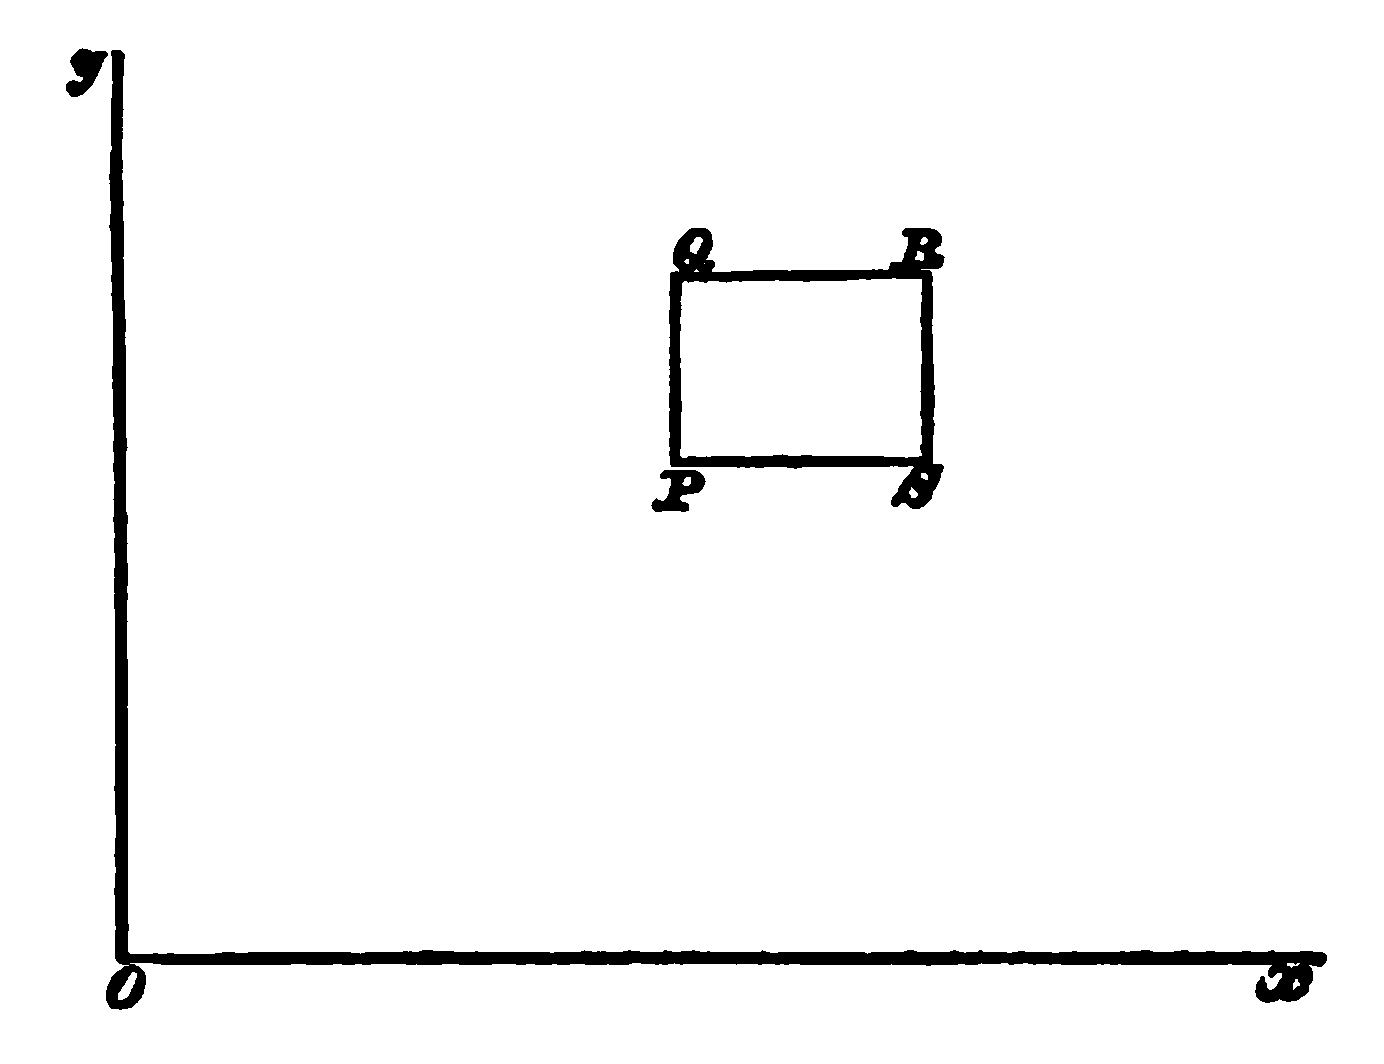
\includegraphics[width=0.6\textwidth]{305.png}
\centering
\end{figure}

Let the coordinates of any point \(P\) be \(x\) and \(y\); let the coordinates
of an adjacent point \(R\) be \(x + h\) and \(y + k\). Complete the
rectangle \(PQRS\), having its sides parallel to the axes.

Let \(\rho\) be the density at \(P\), let \(\rho_{1}\) be the mean density along \(PQ\),
and \(\rho_{2}\) the mean density along \(PS\).

Let \(p\) be the pressure at \(P\); then the pressure at \(Q\) will ultimately
be \(p + \rho_{1} Yk\), and the pressure at \(S\) will ultimately be
\(p + \rho_{2} Xh\). Now we may form two expressions for the pressure at
\(R\), one obtained by passing from \(Q\) to \(R\), and the other obtained
by passing from \(S\) to \(R\). The former expression is ultimately
\[p + \rho_{1} Yk + \rho_{2} Xh + \frac{d}{dy} (\rho_{2} Xh)k\text{,}\]
and the latter is
\[p + \rho_{2} Xh + \rho_{1} Yk + \frac{d}{dx} (\rho_{1} Yk)h\text{;}\]
equate these and we obtain ultimately
\[\frac{d}{dx}(\rho_{1} Y) = \frac{d}{dy}(\rho_{2} X)\text{,}\]
that is
\[\frac{d}{dx}(\rho Y) = \frac{d}{dy}(\rho X)\text{.}\]

This mode of giving as it were a physical interpretation to the
condition just obtained might be called D'Alembert's hydrostatical
%%-----File: 306.png-----%%
principle; though it is not very clearly put by himself. We may
say verbally that the principle amounts to this: the change of
pressure in passing from one given point of a fluid in equilibrium
to another is independent of the path by which we proceed.

\Section
395. An Appendix entitled \textit{Réflexions sur les loix de l'Equilibre
des Fluides} occupies pages 190\dots 212 of the work.

D'Alembert gives on his pages 190\dots 194 another demonstration
of the equation \(\xp\dfrac{d}{dx} (\rho Y) = \xp\dfrac{d}{dy} (\rho X)\); this demonstration is sound
but complex: he gives it, he says, because it will supply the opportunity
for some important remarks on the laws of the equilibrium
of fluids. The remarks do not seem to me of great importance;
but the reader can judge for himself from the account which will
now be given of them.

\Section
396. D'Alembert says on his page 195, in effect, that if with
previous writers on this subject we suppose the density to be constant
throughout every level surface we arrive at the equation
\(\xp\dfrac{dY}{dx} = \xp\dfrac{dX}{dy}\) instead of that in Art.\ 394: this appears to him to require
explanation. Along a surface of equal density we have
\(\xp\dfrac{d\rho}{dx} dx + \xp\dfrac{d\rho}{dy} dy = 0\); if this surface is also a level surface we have
\(Xdx + Ydy = 0\); hence \(Y \xp\dfrac{d\rho}{dx} = X \xp\dfrac{d\rho}{dy}\), and the equation of Art.\ 394
reduces to \(\xp\dfrac{dY}{dx} = \xp\dfrac{dX}{dy}\). So far he is right, but he adds a remark
which is quite erroneous; changing his notation to that which we
have used, his words are:

\begin{squote}
Mais il faut remarquer que l'équation \(\xp\dfrac{dX}{dy} = \xp\dfrac{dY}{dx}\) n'a lieu dans ce cas
que pour les couches \dots\ auxquelles la direction de la pesanteur est perpendiculaire,
au lieu que l'équation \(\xp\dfrac{d}{dx} (\rho Y) = \xp\dfrac{d}{dy} (\rho X)\) a lieu généralement
pour telle couche qu'on voudra\dots.
\end{squote}

This is a strange error: from the nature of the equation
\(\xp\dfrac{dY}{dx} = \xp\dfrac{dX}{dy}\) it is quite independent of direction.
%%-----File: 307.png-----%%

\Section
397. D'Alembert says on his page 197, that the equation of
Art.\ 394 supposes \(\rho\), \(X\), and \(Y\) to be functions of \(x\) and \(y\): but he
does not see why we should be restricted to this hypothesis. He
proceeds to something which he considers more general, but which
is really not so; in fact he supposes that \(X\) and \(Y\) are functions of
\(x\), \(y\), and \(\zeta\) where \(\zeta\) is itself a definite function of \(x\) and \(y\): but it
is obvious that this is practically identical with the usual hypothesis.
I found after I had written this that Lagrange had made an
equivalent remark in the \textit{Miscellanea Taurinensia}, Vol.\ \textsc{ii}.\ page 282.
D'Alembert himself also subsequently admitted that this introduction
of \(\zeta\) was superfluous: see his \textit{Opuscules Mathématiques},
Vol.\ \textsc{viii}.\ page 16.

\Section
398. D'Alembert makes an erroneous statement on his page 199,
namely, that if the pressure be equal at all points of the
bounding surface the force must be equal at all points: we know
that this is not necessarily the case. Indeed D'Alembert himself
says on his page 201:

\begin{squote}
\dots\ A l'égard du principe de l'égalité des forces, il est évident que s'il
étoit admis, toutes les Théories qu'on a données de la Figure de la Terre,
en la considérant comme un Fluide, et en ayant égard à l'attraction des
parties, et à la rotation de l'Axe, devroient être regardées comme fausses.
\end{squote}

\Section
399. D'Alembert returns to the matter which we noticed in
Art.\ 367; and seems still half persuaded of the truth of the absurd
opinion stated there. However he converts himself from his error
by the aid of an important principle which he had formerly given.
The following is the substance of his argument: it is obvious that
a fluid may be in motion without having its surface plane or
spherical; and it follows from what we now call \textit{D'Alembert's
Principle} that if any motion is known we know also the forces
which would maintain the system in equilibrium in the configuration
which it has at any instant; thus forces do exist which would
maintain a fluid in equilibrium and give to the surface a form
which is neither plane nor spherical.

\Section
400. D'Alembert seems to attach great importance to the
fact that if a fluid be in equilibrium the surfaces of equal density
%%-----File: 308.png-----%%
are not necessarily level surfaces. We know now, with the usual
notation, that if \({Xdx + Ydy + Zdz}\) is a perfect differential, the
surfaces of equal density will be level surfaces; moreover for such
forces as occur in nature this condition is satisfied: hence for such
cases as occur in nature it is true that the surfaces of equal density
are level surfaces. But D'Alembert's statement is correct, that
surfaces of equal density are not necessarily level surfaces. See
Arts.\ 315 and 368.

\Section
401. We will give briefly the example which D'Alembert
discusses, translating his process into modern language.

Suppose \(s\) the distance of a point from the origin, and \(\theta\) the
angle which \(s\) makes with a fixed straight line. Let \(S\) denote the
force along \(s\), and \(T\) that at right angles to \(s\); and let \(\sigma\) denote
the density.

Then the usual equations for the equilibrium of a fluid are
\[\frac{dp}{ds}=\sigma S,\qquad \frac{dp}{sd \theta} = \sigma T,\]
where \(p\) denotes the pressure. Therefore
\[\frac{d}{d\theta} (\sigma S) = \frac{d}{ds} (\sigma sT)\tag{1}.\]

This condition in fact agrees with what D'Alembert himself
deduces from the principle of canals.

Now let us assume that the fluid is arranged in strata of equal
density; let the curve of equal density be determined by the
equation
\[s = r + \alpha\rho Z\tag{2},\]
where \(r\) is a parameter which particularises the curve we consider,
\(\rho\) is a function of \(r\), and \(Z\) a function of \(\theta\); and \(\alpha\) is a very small
quantity, the square of which will be neglected.

Also suppose that
\[-S = \rho' + \alpha \rho'' Z',\quad\text{and}\quad T = \alpha \rho''' Z''\tag{3},\]
where \(\rho'\), \(\rho''\), and \(\rho'''\) are functions of \(r\); and \(Z'\) and \(Z''\) are
functions of \(\theta\). The notation is kept very close to D'Alembert's,
though not exactly the same.
%%-----File: 309.png-----%%

Now (1) may be written
\[S \frac{d\sigma}{d\theta} + \sigma \frac{dS}{d\theta} = \sigma T + sT \frac{d\sigma}{ ds} + \sigma s \frac{dT}{ds} \tag{4}.\]

The condition that \(\sigma\) is constant along the curves determined
by (2) gives
\[\frac{d\sigma}{d\theta} + \frac{d\sigma}{ds}\frac{ds}{d\theta} = 0,\]
that is,
\[\frac{d\sigma}{d\theta} + \alpha\rho \frac{dZ}{d\theta}\frac{ d\sigma}{ds} = 0.\]

Then (4) becomes
\[-\left(S\alpha\rho\frac{ dZ}{d\theta} + sT\right)\frac{d\sigma}{ds} = \sigma T - \sigma \frac{dS}{d\theta} + \sigma s \frac{dT}{ds}.\]

Substitute from (3), and neglect the square of \(\alpha\); thus
\[\alpha\left(\rho\rho' \frac{dZ}{d\theta} - s\rho''' Z''\right)\frac{d\sigma}{ds} = \alpha\sigma\rho''' Z'' - \sigma \frac{dS}{d\theta} + \alpha\sigma sZ'' \frac{d\rho'''}{dr} \tag{5}.\]

Here \(\xp\dfrac{dS}{d\theta}\) means the differential coefficient of \(S\) with respect
to \(\theta\), supposing \(s\) constant; and so it is found by combining
\begin{align*}
-\frac{dS}{d\theta} &= \left(\frac{d\rho'}{dr} + \alpha Z' \frac{d\rho''}{dr}\right)\frac{dr}{d\theta} + \alpha\rho'' \frac{dZ'}{d\theta},\\
\shortintertext{and}
0 = \frac{ds}{d\theta} &= \left(1 + \alpha Z \frac{d\rho}{dr}\right)\frac{dr}{d\theta} + \alpha\rho \frac{dZ}{d\theta}.
\end{align*}

Hence, neglecting the square of \(\alpha\),
\[-\frac{dS}{d\theta} = -\alpha\rho \frac{d\rho'}{dr}\frac{dZ}{d\theta} + \alpha\rho'' \frac{dZ'}{d\theta};\]
also if we neglect the square of \(\alpha\) we may put \(\xp\dfrac{d\sigma}{dr}\) for \(\xp\dfrac{d\sigma}{ds}\) in (5).
Then, dividing by \(\alpha\), we obtain
\[\left(\rho\rho' \frac{dZ}{d\theta} - r\rho''' Z''\right) \frac{d\sigma}{dr} = \sigma\rho''' Z'' - \sigma\rho \frac{d\rho'}{dr}\frac{ dZ}{d\theta}
+ \sigma\rho'' \frac{dZ'}{d\theta} + \sigma rZ'' \frac{d\rho'''}{dr}\tag{6}.\]
%%-----File: 310.png-----%%

\Section
402. We will make some remarks on the equation (6).
D'Alembert himself by transposition puts it in this form:
\[\frac{dZ}{d\theta}\frac{d}{dr} (\sigma \rho \rho') - Z'' \frac{d}{dr} (\sigma r \rho''') = \sigma \rho'' \frac{dZ'}{d\theta} + \sigma \rho' \frac{d\rho}{dr} \frac{dZ}{d\theta}.\]

D'Alembert obtains this result by the method which we have
exemplified in Art.\ 394. In modern language we may say that he
passes from one point of the fluid to another by two different
routes; and thus he obtains two expressions for the change of
pressure, which can be equated. But as he does not use the
word \textit{pressure}, or the symbol \(p\), his method is somewhat obscure.
In the diagram of Art.\ 394, we see that
\begin{gather*}
\text{the increase of pressure from \(P\) to \(Q\) + increase from \(Q\) to \(R\)}\\
= \text{increase from \(P\) to \(S\) + increase from \(S\) to \(R\).}
\end{gather*}

With D'Alembert the equivalent statement takes the less
natural form,
\begin{gather*}
\text{the increase of pressure from \(Q\) to \(R\) - increase from \(P\) to \(S\)}\\
= \text{increase from \(S\) to \(R\) - increase from \(P\) to \(Q\).}
\end{gather*}

Instead of the words \textit{increase of pressure from \(P\) to \(Q\)},
D'Alembert uses such words as \textit{force of the column \(PQ\) along \(PQ\)};
and these seem scarcely intelligible. D'Alembert attempts to
enunciate this case of his hydrostatical principle in words in his
\textit{Recherches \dots\ Systême du Monde}, Vol.\ \textsc{iii}.\ page 226, where he says:

\begin{squote}
\dots\ il faut supposer la différence de pesanteur de deux couches de
niveau infiniment proches, égale à la différence de pesanteur de deux
couches verticales infiniment proches,\dots
\end{squote}

An enunciation, partly in words and partly by symbols, is also
given by Lagrange; see the \textit{Miscellanea Taurinensia}, Vol.\ \textsc{ii}.\
page 285.

We may remark that D'Alembert's notation might be rendered
at once simpler and more general. Instead of \(\rho Z\), where \(\rho\) is a
function of \(r\) and \(Z\) a function of \(\theta\), put \(V\), where \(V\) is a function
of both \(r\) and \(\theta\); also put \(V'\) instead of \(\rho'' Z'\), and \(V''\) instead of
\(\rho''' Z''\). Then the equation at the beginning of this Article may
be written
\[\frac{dV}{d\theta}\frac{d}{dr} (\sigma \rho') - \frac{d}{dr} (\sigma r V'') = \sigma \frac{dV'}{d \theta}.\]
%%-----File: 311.png-----%%

In his \textit{Opuscules Mathématiques}, Vol.\ \textsc{v}.\ page 6, D'Alembert
returns to the example of Art.\ 401. There he takes \(\rho'\) to be a
function of \(s\) instead of \(r\); or, which comes to the same thing to
his order of approximation, he puts instead of the first of equations
(3)
\[- S = \rho' + \frac{d \rho'}{dr} \alpha \rho Z + \alpha \rho'' Z';\]
hence we have an additional term \(\alpha \xp\dfrac{d \rho'}{dr} \rho \xp\dfrac{dZ}{d\theta} \sigma\) on the right-hand
side of (5): and finally, instead of (6), we obtain
\[\rho \rho' \frac{dZ}{d \theta} \frac{ d \sigma}{dr} - Z'' \frac{d}{dr} (\sigma r \rho''') = \sigma \rho'' \frac{dZ'}{d \theta}.\]

\Section
403. I am not sure that I understand D'Alembert's continuation
after the point which we reached at the end of Art 401;
but I think that it is substantially equivalent to the following.

Assume that the surfaces of equal density are level surfaces;
then the force along the tangent to the curve considered must
vanish. Thus we obtain to our order of approximation
\[\frac{\rho \rho'}{r} \frac{dZ}{d \theta} = \rho''' Z''.\]

Now \(\rho'\) and \(\rho\) are functions of \(r\) only, and \(Z\) and \(Z'\) are functions
of \(\theta\) only; so we must have
\[\frac{\rho \rho'}{r} = C \rho''',\qquad Z'' = C \frac{dZ}{d \theta}\tag{7},\]
where \(C\) is some constant.

Substituting in (6) we obtain
\[\left\{ C \left(\rho''' + r \frac{d \rho'''}{dr}\right) - \rho \frac{d \rho'}{dr}\right\} \frac{dZ}{d \theta} + \rho'' \frac{dZ'}{d \theta} = 0;\]
which, as before, leads to
\[\frac{dZ'}{d \theta} = B \frac{dZ}{d \theta},\qquad C\left(\rho''' + r \frac{d \rho''' }{dr}\right) - \rho \frac{d \rho' }{ dr} = - B \rho'' \tag{8},\]
where \(B\) is some constant.

Thus we have the four equations (7) and (8) holding in place
of the single equation (4).
%%-----File: 312.png-----%%

From the first of (8) we have
\[Z' = BZ + B',\]
where \(B'\) is some constant.

From the first of (7) and the second of (8) we get
\[\frac{d(\rho' \rho)}{dr} - \rho \frac{d\rho'}{dr} = - B \rho'',\]
so that
\[-B \rho'' = \rho' \frac{d\rho }{dr}.\]

Thus, finally,
\[s = r + \alpha \rho Z,\quad -S = \rho' - \frac{\alpha}{B} \rho' \frac{d\rho}{dr} (BZ + B'),\quad T = \frac{\alpha \rho \rho' }{rC} C \frac{dZ}{d\theta},\]
that is,
\[s = r + \alpha \rho Z,\quad -S = \rho' - \alpha \rho'\frac{d\rho}{dr} (Z + B_1),\quad T =\frac{ \alpha \rho \rho' }{r} \frac{dZ}{d\theta},\]
where \(B_1\) is some constant.

These results are of course less general than the single equation
(4).

\Section
404. D'Alembert finishes the Appendix with some matter
which is very closely connected with our subject. He says on
his pages 208 and 209:

\begin{squote}
Je remarquerai à cette occasion, qu'il me semble qu'on n'a point
encore résolu d'une maniére assez générale le Problême de la figure de la
Terre, dans l'hypothese que l'attraction soit en raison inverse du quarré
des distances, et que la Terre soit composée d'un amas de Fluides de
différentes densités.
\end{squote}

Accordingly, D'Alembert proposes his more general solution of
the problem of the Figure of the Earth. It would not be advisable
to devote much space to shew that D'Alembert's additions
to Clairaut's investigations are worthless; but as we have already
given the principal formulæ which are necessary, we shall be able
with brevity to justify this opinion. D'Alembert himself refers, as
we shall do, to Clairaut, for some formulæ which are necessary.
%%-----File: 313.png-----%%

We adopt Clairaut's hypothesis that the Earth consists of
ellipsoidal fluid strata of varying density and ellipticity. Let
\(\rho\) denote the density; take the known equation of Art.\ 401,
\[\frac{d}{d\theta}[\rho S] = \frac{d}{ds} [\rho sT]\tag{1}.\]

Here the quantities are supposed to be expressed in terms
of \(\theta\) and \(s\); and we use the square brackets to indicate this.
But suppose that \(s\) is changed into \(r (1 + \epsilon \sin^2 \theta)\); then we have
to transform (1) suitably.
\[\frac{d}{d \theta} [\rho S] = \frac{d}{d\theta} (\rho S) + \frac{d}{dr} (\rho S) \frac{dr}{d\theta},\]
and \(\xp\dfrac{dr}{d \theta}\) is to be found on the supposition that \(s\) is constant, so that
to our order of approximation it is equal to \(-2r\epsilon \sin \theta \cos \theta\).

Thus rejecting the square of \(\epsilon\) we have from (1)
\[\frac{d}{d\theta} (\rho S) - \frac{d}{dr}(\rho S) 2r \epsilon \sin \theta \cos \theta = \frac{d}{dr} (\rho rT).\]

Let \(\phi\) denote the angle between the radius vector and the
tangent to the ellipse at the point considered; so that to our
order \(\cos \phi = 2 \epsilon \sin \theta \cos \theta\). Hence
\begin{multline*}
\frac{d}{d \theta} (\rho S) = \frac{d}{dr} (\rho rT) + r \cos \phi \frac{d}{dr} (\rho S)\\
= \frac{d}{dr} \rho (rT + r \cos \phi S) - 2 \sin \theta \cos \theta \rho S \frac{d(r \epsilon)}{dr}.
\end{multline*}

Thus
\[\frac{d}{d \theta} (\rho S) + 2 \rho \sin \theta \cos \theta S \frac{d(r \epsilon)}{dr} = \frac{d}{ dr} (\rho r Q),\]
where \(Q\) stands for \(T + \cos \phi S\), that is, for the whole force
along the tangent; and the first term may be written \(\rho \xp\dfrac{dS}{d \theta}\).
Hence finally
\[\rho \frac{dS}{d \theta} + 2 \rho \sin \theta \cos \theta S \frac{d(r \epsilon)}{dr} = \frac{d}{dr} (\rho rQ)\tag{2}.\]

This equation substantially coincides with that which D'Alembert
uses; but he does not sufficiently explain his process.
%%-----File: 314.png-----%%

\Section
405. We have now to give the values of \(Q\) and \(S\). I shall
use the following notation:
\begin{align*}
\Upsilon (r)\quad &\text{for}\quad \int_{0}^{r} {\rho r^2} dr,\\
\Omega_0 (r)\quad &\text{for}\quad \int_{0}^{r} {\rho \frac{d \epsilon}{dr}} dr,\\
\Omega_3 (r)\quad &\text{for}\quad \int_{0}^{r} {\rho \frac{d(r^3 \epsilon)}{dr}} dr,\\
\Omega_5 (r)\quad &\text{for}\quad \int_{0}^{r} {\rho \frac{d(r^5 \epsilon)}{dr}} dr\text{.}
\end{align*}

Let \(b\) be the extreme value of \(r\), that is the value of \(r\) at
the surface; and let \(\omega\) be the angular velocity. Then it will be
found that
\[
Q = \sin \theta \cos \theta \left\{- \frac{8 \pi \epsilon \Upsilon (r)}{r^2} + \frac{8 \pi \Omega_5 (r)}{5r^4} + \frac{8 \pi r}{5} [\Omega_0 (b) - \Omega_0 (r)] + \omega^2 r\right\}
\]
\begin{multline*}
-S = \frac{4 \pi (1-2 \epsilon \sin^2 \theta)}{r^2} \Upsilon (r) + \frac{8 \pi}{3r^2} \Omega_3 (r)\\
+ 4 \pi (3 \sin^2 \theta - 2) \left\{\frac{ \Omega_5 (r)}{5r^4} - \frac{\Omega_0 (b) - \Omega_0 (r)}{15} 2r \right\} - \omega^2 r \sin^2 \theta.
\end{multline*}

The value of \(Q\) is found as in Art.\ 341, or Clairaut's page 273.
The value of \(-S\) is found as in Art.\ 336, or Clairaut's page 247:
it is only necessary to add to what is there given the central
attraction which arises from the matter which may be said to
be external to the attracted point, and thus we obtain the term
which involves \(\Omega_0\) in the manner the term involving \(\Omega_5\) was
obtained.

Hence \(-\xp\dfrac{dS}{d \theta}\)
\[
= \sin \theta \cos \theta \left\{ - \xp\dfrac{16 \pi \epsilon \Upsilon (r)}{r^2} + \xp\dfrac{24 \pi \Omega_5 (r)}{5r^4} - \xp\dfrac{16 \pi r}{5} [\Omega_0 (b) - \Omega_0 (r)] - 2 \omega^2 r \right\}.
\]

Thus (2) becomes to our order of approximation
\begin{multline}
\rho \left\{\frac{\Upsilon (r)}{r^2}\frac{d(r \epsilon)}{dr} - \frac{2 \epsilon}{r^2} \Upsilon (r) + \frac{3 \Omega_5 (r)}{5r^4} -\frac{2r}{ 5} [\Omega_0 (b) -\Omega_0 (r)] - \frac{\omega^2 r}{4\pi}\right\}\\
=\frac{d}{dr} \rho \left\{\frac{\epsilon \Upsilon (r)}{r} - \frac{\Omega_5 (r)}{5r^3} - \frac{r^2}{5} [\Omega_0 (b) - \Omega_0 (r)]- \frac{\omega^2 r^2 }{8 \pi}\right\} \tag{3}.
\end{multline}
%%-----File: 315.png-----%%

Let \(K = \xp\dfrac{\epsilon}{r^2} \Upsilon(r) - \xp\dfrac{\Omega_5(r)}{5r^4} - \xp\dfrac{r}{5} [\Omega_0(b) - \Omega_0(r)] - \xp\dfrac{\omega^2 r }{ 8 \pi}\); then multiply
by \(r^4\) and differentiate; then divide by \(r^4\) and differentiate again.
Thus we obtain
\[\frac{d^2 \epsilon}{dr^2} + \frac{2 \rho r^2}{\Upsilon(r)}\frac{ d\epsilon}{dr} - \left\{\frac{6}{r^2} - \frac{2 \rho r}{ \Upsilon(r)}\right\} \epsilon = \frac{r^2}{\Upsilon(r)}\frac{ d}{dr} \left\{\frac{1}{r^4} \frac{d}{ dr} (Kr^4)\right\} \tag{4}.\]

Moreover (3) may be written
\[\frac{d}{dr} (K r \rho) = \rho \left\{\frac{d(r \epsilon)}{dr}\frac{\Upsilon(r)}{r^2} - \frac{4\epsilon\Upsilon(r)}{r^2} + \frac{\Omega_5(r)}{r^4} + 2K\right\};\]
multiply by \(\xp\dfrac{r^4}{\rho}\) and differentiate: then we obtain
\[
\frac{d^2\epsilon}{dr^2} + \frac{2 \rho r^2}{\Upsilon(r)} \frac{d\epsilon}{dr} - \left\{\frac{6}{r^2} - \frac{2 \rho r}{ \Upsilon(r)}\right\} \epsilon
= \frac{1}{r^3 \Upsilon(r)}\left[\frac{d}{dr}\left\{\frac{r^4}{\rho} \frac{d(K r \rho)}{dr} - 2Kr^4\right\}\right] \tag{5}.
\]

Comparing (4) and (5) we obtain \({\xp\dfrac{d}{dr}\left(\dfrac{Kr^5}{\rho} \dfrac{d\rho}{dr}\right) = 0}\); therefore
\(\xp\dfrac{Kr^5}{\rho}\dfrac{d\rho}{dr} = M\) a constant; and so the right-hand side of (4) becomes
\[\frac{r^2}{\Upsilon(r)}\frac{d}{dr}\left\{\frac{1}{r^4}\frac{d}{dr}\left(\frac{M \rho}{r} \frac{dr}{d\rho}\right)\right\}.\]

Thus D'Alembert considers he has found a more general result
than had hitherto been given; for we know that Clairaut's \textit{derived
equation} agrees with (4) when the right-hand side is changed
to zero: see Art.\ 343.

But D'Alembert himself admits, that at the external surface
there can be no tangential force, and so \(K\) must vanish there; see
the last line of his page 211. This would suggest \(M = 0\); but
D'Alembert wishes to avoid this, and so he says it will be sufficient
to have \(\xp\dfrac{d\rho}{dr}\) infinite at the external surface.

The error involved is very serious even for D'Alembert: such
a strange result should have led him to review his process. If we
develope the right-hand side of (3) we have one term involving
%%-----File: 316.png-----%%
\(\xp\dfrac{d\rho}{dr}\), and another involving \(\rho\); the latter term is exactly the same
as we have on the left-hand side of (3). Thus (3) becomes simply,
in D'Alembert's notation, \(K r \xp\dfrac{d\rho}{dr} = 0\); thus either \(K = 0\), or \(\xp\dfrac{d\rho}{dr} = 0\);
in the latter case the density is constant: in both cases the level
surfaces are surfaces of equal density.

In fact, as we stated in Art.\ 400, we know that for such forces
as occur in nature the level surfaces must be surfaces of equal
density; this was pointed out by Lagrange in some observations on
D'Alembert's misconception: see the \textit{Miscellanea Taurinensia},
Vol.\ \textsc{ii.}\ page 285.

\Section
406. D'Alembert himself briefly admitted and corrected his
error in his \textit{Opuscules}, Vol.\ \textsc{v.}\ page 4: my remarks were written
before I had arrived at this admission; and I have ventured to
retain them. It is curious to notice the complacent satisfaction
with which D'Alembert, up to the period of the admission of his
error, regarded his efforts to improve the important result which
I call Clairaut's derived equation: see the \textit{Recherches \dots\ Systême
du Monde}, Vol.\ \textsc{ii.}\ page 290, and Vol \textsc{iii.}\ pages xxxvi and xxxvii;
and also the article \textit{Figure de la Terre} in the original \textit{Encyclopédie}.

\Section
407. We might have deduced equation (3) of Art.\ 405 from
equation (6) of Art.\ 401. Return to the notation of Art.\ 401, using
\(\sigma\) for the density. We have
\[
\frac{dZ}{d\theta} = \frac{dZ'}{d\theta} = Z'' = 2 \sin\theta \cos\theta;
\]
and thus equation (6) becomes
\[
\frac{d}{dr} \sigma(\rho\rho' - r\rho''') = \sigma\rho'' + \sigma\rho'\frac{d\rho}{dr};
\]
and
\[
\alpha\rho = r\epsilon, \quad \rho' = 4\pi \left\{\frac{\Upsilon(r)}{r^2} + \text{small terms}\right\},
\]
\[
\alpha\rho'' = 4\pi \left\{- \frac{2\epsilon\Upsilon(r)}{r^2} + \frac{3\Omega_{5}(r)}{5r^4} - \frac{2r}{5}[\Omega_{0}(b) - \Omega_{0}(r)] - \frac{\omega^2 r}{4\pi} \right\},
\]
\[
\alpha\rho''' = 4\pi \left\{\frac{\Omega_{5}(r)}{5r^4} + \frac{r}{5}[\Omega_{0}(b) - \Omega_{0}(r)] + \frac{\omega^2 r}{8\pi} \right\}\text{.}
\]
%%-----File: 317.png-----%%

Substitute these values in the above equation, and it will be
found to agree with (3) of Art.\ 405.

\Section
408. In considering the writings of D'Alembert on our subject
up to the present point, we find but little of importance. Not
only do they fail to add anything to what Clairaut had given, but
they do not even reach the same level. It seems to me that
D'Alembert had not taken the trouble to study a work which far
surpassed all his own efforts in the same direction.

\Section
409. The next work by D'Alembert is entitled \textit{Recherches sur
différens points importans du Systême du Monde}. This work forms
three parts or volumes in quarto. The first and the second parts
were published in 1754; and the third part in 1756.

The first part contains the Title, Preliminary Essay, Table of
Contents, and Corrections in lxviii pages; then the text of
260 pages: there is one plate.

The second part contains the Title and Table of Contents in
vi pages; then the text of 290 pages: there are three plates.

The third part contains the Title, Preface, Table of Contents,
and the \textit{Privilege du Roi} in xlviii pages; then the text and Corrections
of 263 pages: there are two plates.

\Section
410. There is nothing in the first part with which we are
concerned.

In the second part we have on pages 201\dots 209, \textit{Remarques
sur la figure de la Terre, qui résulte de la Précession des Equinoxes};
and on pages 265\dots 290, we have a Chapter entitled \textit{De la Figure
de la Terre}.

\Section
411. D'Alembert, on his pages 201\dots 209, returns to the subject
of the information which the theory of the Precession of the Equinoxes
gives with respect to the theory of the Figure of the Earth.
He first substantially repeats the matter of which we have
given an account in Arts.\ 385 and 386. He then says, on his
page 204:

\begin{squote}
Je dois cependant avouer qu'un grand Geométre a cru pouvoir
concilier tout, en supposant que la Terre soit un solide Elliptique, dont
%%-----File: 318.png-----%%
la différence des Axes soit \(= \xp\dfrac{1}{200}\), et qui renferme au-dedans de lui un
noyau sphérique dont la densité soit à celle du Sphéroide comme \(10\) est
à \(1\), et dont le rayon soit au rayon de l'Equateur comme \(3\) à \(5\).
\end{squote}

D'Alembert here alludes to a memoir by Euler on the Precession
of the Equinoxes, published in the Berlin \textit{Mémoires} for
1749; see page 315 of the memoir: Euler does not support his
suggestion by any theory connected with our subject.

D'Alembert shews that the above supposition is inadmissible.
Take a formula obtained in Art.\ 374, namely
\[
\epsilon = \frac{ \dfrac{r\omega^2}{2}} {\dfrac{4\pi\rho r}{3} + \dfrac{4\pi (\sigma - \rho) s^3}{3r^2} - \dfrac{4\pi\rho r}{5}};
\]
let \(j\) denote, as usual, the ratio of the centrifugal force at the
equator to the attraction there, so that
\[
r\omega^2 = j \left\{ \frac{4\pi\rho r}{3} + \frac{4\pi(\sigma - \rho)s^3}{3r^2} \right\};
\]
therefore
\[
\epsilon = \frac{\dfrac{j}{2} \left\{\rho + (\sigma - \rho) \dfrac{s^3}{r^3}\right\} } {\rho + (\sigma - \rho) \dfrac{s^3}{r^3} - \dfrac{3\rho}{5}}\text{.}
\]

Now let us suppose \(\sigma = 10\rho\), and \(s = \xp\dfrac{3}{5} r\), so that \(\xp\dfrac{(\sigma - \rho)s^3}{\rho r^3} = 2\)
very nearly. Thus
\[
\epsilon = \frac{j}{2} \frac{1 + 2}{1 + 2 - \dfrac{3}{5}} = \frac{5j}{8};
\]
this value of \(\epsilon\) is smaller than observation will allow. It will be
observed that D'Alembert assumes that the ellipticity of the external
surface is the same as if the outer part were \textit{fluid}: it is
not obvious whether Euler contemplated this in his hypothesis
that the Earth consisted of two \textit{solid} parts.

\Section
412. We now pass to pages 265\dots 290 of the volume. On
pages 265\dots 274, D'Alembert considers how the figure of the Earth
%%-----File: 319.png-----%%
may be found by geographical operations. He suggests in fact
that we should assume for the radius vector a series with unknown
coefficients involving cosines of multiples of the colatitude. Then
by measuring the lengths of degrees of the meridian in various
latitudes we find the corresponding values of the radius of curvature:
and thus we obtain equations for determining the unknown
coefficients in the assumed expression for the radius vector.

\Section
413. D'Alembert also suggests that observations of the Moon's
parallax may be employed for information as to the figure of the
Earth: but he admits that practically this method would be of
little value.

\Section
414. In pages 275\dots 290, D'Alembert indicates a method for
calculating the attraction of a spheroid on a particle at the surface.
Suppose \(Q\) a point of the surface, \(C\) the point which may be
called the centre of the spheroid. D'Alembert proposes to consider
the spheroid as composed of two parts; one part being the
sphere on \(CQ\) as radius, and the other part the difference between
the sphere and the spheroid. He shews how the approximate
value of the attraction of the second part may be conveniently
calculated.

It is obvious that the principle of this method is the same as
that which has since been developed by Laplace. D'Alembert
gives only an outline of his method here; he works it out in
detail in the third volume of the \textit{Recherches \dots\ Systême du Monde}.
We shall recur to it in our Article 424.

\Section
415. We now arrive at the third volume of the \textit{Recherches \dots\ Systême
du Monde}. Here pages xix\dots xlii and 107\dots 260 are
devoted to the Figure of the Earth.

\Section
416. In pages xix\dots xlii D'Alembert gives some introductory
remarks on the subject, the purport of which is to shew the uncertainty
as to the actual facts. It was possible to doubt whether
the Earth was a figure of revolution; granting it to be such, it
was possible to doubt whether the northern and the southern
hemispheres were exactly alike; and granting that they were
%%-----File: 320.png-----%%
exactly alike, it was possible to doubt whether the figure was that
of an ellipsoid of revolution.

D'Alembert refers to six measured lengths which had to be
considered in testing any theory; five of these were arcs of
meridians, namely, those in Lapland, Peru, France, the Cape
of Good Hope, and Italy: one was an arc of longitude, in latitude
\(43°\,32'\). As to a degree of the meridian in France, three lengths
had been proposed; Picard gave \(57060\) toises; the Academicians
of the North corrected it to \(57183\) toises; and subsequently it
was put at \(57074\) toises: see Art.\ 236.

D'Alembert found it impossible to assign such a value of the
ellipticity as would harmonise the six measured lengths.

\Section
417. The following points of interest may be noticed in the
introductory remarks by D'Alembert.

On page xxxii he says that a hemispherical mountain a league
high ought to make a pendulum deviate more than \(1'\) from the
vertical; but the high mountains in Peru scarcely produced a
variation of \(7''\). It is easy to verify his calculation, supposing the
density of the mountain equal to the mean density of the Earth.
For the facts as to the mountains in Peru see Bouguer's \textit{Figure
de la Terre}, pages 364\dots 394.

D'Alembert in a note on his page xl suggests, that in such a
mountainous country as Italy, the direction of the plumb-line
may have been disturbed, and thus an error produced in the
measured length of a degree.

D'Alembert refers to the figure of Jupiter as suggesting by
analogy what the figure of the Earth may be; but I do not understand
all that is said on this matter. The following passage
occurs on pages xxxv and xxxvi.

\begin{squote}
Car les observations nous prouvent que la surface de Jupiter est
sujette à des altérations sans comparaison plus considérables et plus
fréquentes que celle de la Terre; or si ces altérations n'influoient en
rien sur la figure de l'équateur de Jupiter, pourquoi la figure de l'équateur
de la Terre seroit-elle altérée par des mouvemens beaucoup
moindres?
\end{squote}

I do not know what changes in Jupiter he refers to here.
%%-----File: 321.png-----%%

Again he suggests that we should determine by observation
whether the figure of Jupiter is precisely that which theory would
assign; but I cannot see any practical value in the method
which he proposes. He states it thus on his page xli:

\begin{squote}
Pour cela il suffiroit de mesurer le parallele à l'équateur de Jupiter,
qui en seroit éloigné de 60 degrés; si ce parallele se trouvoit sensiblement
égal ou inégal à la moitié de l'équateur, le méridien de Jupiter
seroit elliptique ou ne le seroit pas.
\end{squote}

It seems to me that supposing the observation could be made
with great accuracy it would afford but little information; if the
parallel were not exactly half of the equator, we should know
that the meridian could not be circular: but we could not in any
case pronounce what the figure must be from merely knowing
the value of this parallel.

\Section
418. We now proceed to the text on pages 107\dots 260.

A brief introduction commences the discussion. D'Alembert
proposes to examine the figure of the Earth, first astronomically,
so far as observations make it known, and then physically by
theory.

\Section
419. In the first three Chapters D'Alembert considers whether
we can by direct observations determine if certain hypotheses
which are usually made are strictly true. Thus, for example, we
usually assume that the plane which contains the axis of the
Earth and any given place will also contain the vertical line at
that place: this amounts practically to assuming that the Earth
is a figure of revolution. D'Alembert shews that, strictly speaking,
this hypothesis may be untrue; for observations made at any
given place would not enable us to decide that the vertical did or
did not lie exactly in the plane containing the place and the axis
of the Earth. Again, we define the vertical direction at any
place as that of falling bodies; and we know that this direction
is perpendicular to the surface of fluid at rest at the place: but
this direction will not be necessarily perpendicular to the surface
of the solid Earth at the place. Now D'Alembert shews that if
the angle between these two directions is very small we shall not
be able to detect it by observations.
%%-----File: 322.png-----%%

I do not give any detailed account of these Chapters, since the
propositions are of such a kind that they readily commend themselves
as reasonable. The processes of D'Alembert require attention
to understand them; but they will be found to present no
very serious difficulty.

\Section
420. D'Alembert's fourth Chapter is entitled \textit{De la Figure de
la Terre dans les hypothèses ordinaires}. This is of the same
character as the portion of the second volume of the \textit{Recherches}
which we described in Art.\ 412.

\Section
421. D'Alembert's fifth Chapter is entitled \textit{Des parallaxes en
tant qu'elles dépendent de la figure de la Terre}. The Earth
being not a sphere the parallax of the Moon will vary with the
place of observation; D'Alembert investigates formulæ for the
parallax: but these investigations belong rather to Plane Astronomy
than to Physical Astronomy.

\Section
422. We now pass to D'Alembert's second Section, which is
entitled \textit{De la figure de la Terre considérée physiquement}.

\Section
423. The first Chapter, on pages 166\dots 177, contains the investigation
of certain integrals which will be used in the sequel.

Thus, to take the first, required
\[
\int \frac{dt}{\xsurd(1-t^2)}.\frac{(1-t^2)^n}{(k^2+t^2-k^2t^2)^{n+1}},
\]
\(n\) being a positive integer.

D'Alembert assumes \(k^2+t^2-k^2t^2 = \xp\dfrac{1}{s+1}\); and then the integral
becomes
\[
- \frac{1}{2(1-k^2)^n} \int \frac{s^n ds}{\xsurd (s-k^2s-k^2s^2)}\text{.}
\]

D'Alembert requires the integral between the limits \(0\) and \(1\)
of \(t\); to these limits correspond \(\xp\dfrac{1-k^2}{k^2}\) and \(0\) for \(s\). He easily
obtains the required result by ordinary methods: we will verify by
%%-----File: 323.png-----%%
assuming \(\sin^2\theta = \xp\dfrac{k^2 s}{1 - k^2}\), which reduces the integral to
\[\frac{1}{k^{2n+1}}\int_0^{\tfrac{\pi}{2}} {\sin^{2n}\theta} d\theta,\]
and the value is
\[\frac{1}{k^{2n+1}}.\frac{(2n-1)(2n-3)\ldots1}{2n(2n-2)\ldots2}.\frac{\pi}{2}.\]
D'Alembert arrives at the same result on his page 170; he apparently
gives twice this value, but he has really taken the integral
twice over.

On his page 171, he professes, I think, to investigate the integral
\[\int\frac{dt}{\xsurd(1-t^2)}.\frac{(1-t^2)^{\tfrac{n}{2}}}{(k^2 + t^2 - k^2t^2)^{\tfrac{n}{2} + 1}},\]
where \(n\) is an odd positive integer; but his printing is not very
distinct. This integral transforms as before into
\[-\frac{1}{2(1-k^2)^{\tfrac{n}{2}}}\int \frac{s^{\tfrac{n}{2}}ds}{\xsurd(s - k^2 s - k^2 s^2)}.\]
It is unnecessary for his purpose to take any notice of the numerical
factor which is here outside the integral sign; and so he
omits it.

He gives three times, namely on his pages 174, 176, and 177,
the following result:
\[\int_0^{2r} {\frac{x(2rx-x^2)^2}{(2rx)^{\frac{3}{2}}}}dx = \frac{16\times8r^3}{5\times7\times9}.\]

\Section
424. D'Alembert's second Chapter, on pages 178\dots 199, is
entitled \textit{De l'attraction d'un sphéroïde sur les corpuscules placés
à sa surface; et de la figure qui en résulte pour ce sphéroïde.}

We begin with a general formula for the attraction of a spheroid
on a particle at the surface, resolved tangentially; we shall
follow D'Alembert as to principle, but we shall simplify the mere
analytical work.
%%-----File: 324.png-----%%

Let there be a point \(Q\) on the surface of a spheroid, let \(s\) be
the distance of \(Q\) from a fixed point which we may call the centre
of the spheroid; let \(\theta\) be the angular distance of \(Q\) from the pole.
It is required to find the attraction of the spheroid at \(Q\), resolved
tangentially.

We assume that the spheroid is a figure of revolution. We
may suppose that the spheroid consists of a sphere of radius \(s\), and
an additional shell: see Art.\ 414. We assume that the shell is
at every point so thin that it may be treated as if it were condensed
on the surface of the sphere of radius \(s\). It is obvious that
we need only consider the shell when we seek the tangential
attraction.

\begin{figure}[!ht]
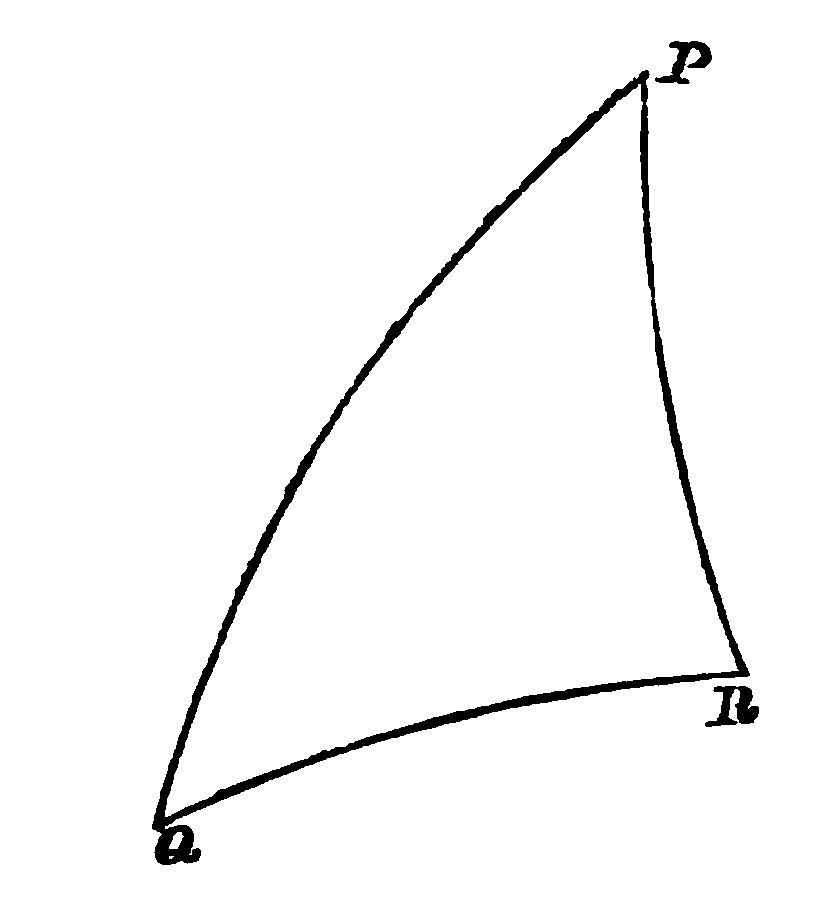
\includegraphics[width=0.35\textwidth]{324.png}
\centering
\end{figure}

Let \(R\) be any other point on the surface of the spheroid; and
let its polar co-ordinates be \(s'\) and \(\theta'\). Let \(P\) be the pole; put \(\mu\)
for the angle which \(QR\) subtends at the centre, and \(\psi\) for the
angle \(PQR\).

The element of spherical surface at \(R\) may be denoted by
\(s^2 \sin \mu\,d\mu\,d\psi\); and thus the element of mass of the shell may be
denoted by \((s'-s) s^2 \sin \mu\,d\mu\,d\psi\), taking the density as unity.
The distance from \(Q\) is \(2s \sin \xp\dfrac{\mu}{2}\). We first take the resolved part
of the attraction along the tangent to \(QR\) at \(Q\); and then we
resolve this along the tangent to \(QP\) at \(Q\).

Thus we obtain
\[(s'-s)s^2 \sin \mu\, d\mu\, d\psi \frac{\cos \dfrac{\mu}{2}}{\left(2s \sin \dfrac{\mu}{2}\right)^2} \cos \psi\text{,}\]
%%-----File: 325.png-----%%
that is
\[\frac{(s'-s) \cos^2 \dfrac{\mu}{2} \cos \psi}{2 \sin \dfrac{\mu}{2}} d\mu\,d\psi\text{.}\]

If we integrate this expression between the limits 0 and \(\pi\)
for \(\mu\), and 0 and \(2\pi\) for \(\psi\), we obtain the tangential attraction
at \(Q\) \textit{towards} the pole.

\Section
425. Now suppose, with D'Alembert, that
\[s' = r + r\alpha (A + B \cos \theta' + C \cos^2 \theta' + D \cos^3 \theta')\text{,}\]
where \(\alpha\) is a very small constant, and \(r\), \(A\), \(B\), \(C\), \(D\) are any constants:
we might suppose these constants connected by the relation
\(A + B + C + D = 0\), and then \(r\) would be the polar semi-axis
of the spheroid. However we will not use this supposition.
Substitute this value of \(s'\) in the expression of the preceding
Article: then we see that the tangential attraction reduces to
\[\frac{\alpha r}{2} \int_{0}^{\pi} \int_{0}^{2\pi} \frac{\cos^2 \dfrac{\mu}{2} \cos \psi}{\sin \dfrac{\mu}{2}} (B \cos \theta' + C \cos^2 \theta' + D \cos^3 \theta')\,d\mu\, d\psi\text{;}\]
and
\[\cos \theta' = \cos \theta \cos \mu + \sin \theta \sin \mu \cos \psi\text{.}\]

We shall determine separately the values of the three parts of
which the integral is composed.

The term involving \(B\) reduces to
\[\frac{\alpha rB}{2} \int_{0}^{\pi} \int_{0}^{2\pi} \frac{\cos^2 \dfrac{\mu}{2} \cos \psi}{\sin \dfrac{\mu}{2}} \sin \theta \sin \mu \cos \psi\,d\mu\,d\psi\text{;}\]
this
\[= \alpha r B \sin \theta\,\pi \int_{0}^{\pi} \cos^2 \frac{\mu}{2} d\mu = \frac{4\pi}{3} \alpha rB \sin \theta\text{.}\]

The term involving \(C\) reduces to
\[\alpha rC \int_{0}^{\pi} \int_{0}^{2\pi} \frac{\cos^2 \dfrac{\mu}{2} \cos \psi}{\sin \dfrac{\mu}{2}} \cos \theta \cos \mu \sin \theta \sin \mu \cos \psi\,d\mu\,d\psi\text{;}\]
this
\[= 2\alpha rC \sin \theta \cos \theta\,\pi \int_{0}^{\pi} \cos^3 \frac{\mu}{2} \cos \mu\, d\mu = \frac{8\pi}{5} \alpha rC \sin \theta \cos \theta\text{.}\]
%%-----File: 326.png-----%%

The term involving \(D\) reduces to
\begin{multline*}
\frac{\alpha rD}{2} \int_{0}^{\pi} \int_{0}^{2\pi} \frac{\cos^2 \dfrac{\mu}{2} \cos \psi}{\sin \dfrac{\mu}{2}} (3 \cos^2 \theta \cos^2 \mu \sin \theta \sin \mu \cos \psi\\
+ \sin^3 \theta \sin^3 \mu \cos^3 \psi)\,d\mu\,d\psi\text{;}
\end{multline*}
this
\[= \alpha rD \sin \theta \cos^2 \theta 3\pi \int_{0}^{\pi}\hspace{-.5em} \cos^3 \frac{\mu}{2} \cos^2 \mu\,d\mu + \alpha rD \sin^3 \theta \frac{3\pi}{4} \int_{0}^{\pi}\hspace{-.5em} \cos^3 \frac{\mu}{2} \sin^2 \mu\,d\mu\]
\[= \frac{76\pi}{35} \alpha rD \sin \theta \cos^3 \theta + \frac{16\pi}{35} \alpha rD \sin^3 \theta\text{.}\]

Thus the whole tangential attraction towards the pole is
\[4\pi\alpha r \left(\frac{B}{3} \sin \theta + \frac{2C}{5} \sin \theta \cos \theta + \frac{19D}{35} \sin \theta \cos^2 \theta + \frac{4D}{35} \sin^3 \theta\right)\text{.}\]

\Section
426. Let there be a solid sphere of radius \(r\) and density \(\sigma\),
surrounded by a thin fluid stratum of density \(\sigma'\); and let the
radius of the external surface of this stratum be the \(s'\) of Art.\ 425.
We propose to enquire if this fluid will remain in a state of relative
equilibrium when rotating with uniform angular velocity.

The attraction towards the centre may be taken as \(\xp\dfrac{4\pi r \sigma}{3}\); the
resolved part of this tangentially towards the pole is found to the
order we require by multiplying by \(\xp\dfrac{ds'}{s'd\theta'}\), using \(\theta\) instead of \(\theta'\) in
the result. Let \(j\) denote the ratio of the centrifugal force at the
equator to the attraction there; then \(\xp\dfrac{4\pi r\sigma}{3} j \sin \theta \cos \theta\) \textit{from} the
pole is the tangential action of the centrifugal force. Thus equating
to zero the whole tangential force we get
\begin{multline*}
4\pi\alpha r \left(\frac{B}{3} \sin \theta + \frac{2C}{5} \sin \theta \cos \theta + \frac{19D}{35} \sin \theta \cos^2 \theta + \frac{4D}{35} \sin^3 \theta\right) \sigma'\\
- \frac{4\pi r\sigma}{3} j \sin \theta \cos \theta - \frac{4\pi\alpha r}{3} (B \sin \theta + 2C \sin \theta \cos \theta + 3D \sin \theta \cos^2 \theta) \sigma = 0\text{.}
\end{multline*}
%%-----File: 327.png-----%%

Divide by \(\sin \theta\); then equate to zero the coefficients of the
various powers of \(\cos \theta\). Thus we obtain
\[\frac{B\sigma'}{3} + \frac{4D\sigma'}{35} - \frac{B\sigma}{3} = 0 \tag{1}.\]
\[\frac{2\alpha C\sigma'}{5} - \frac{j\sigma}{3} - \frac{2\alpha C\sigma}{3} = 0 \tag{2}. \label{426:2}\]
\[\frac{15D\sigma'}{35} - D\sigma = 0 \tag{3}.\]

From (3) we get \(\sigma = \xp\dfrac{3}{7} \sigma'\); then from (2) we get \(\alpha C = \xp\dfrac{5j}{4}\); and
then from (1) we get \(B = - \xp\dfrac{3D}{5}\).

D'Alembert has a wrong equation instead of (1), and so his
value of \(B\) is wrong; he corrects the error in his \textit{Opuscules Mathématiques},
Vol.\ \textsc{vi}.\ page 230.

It is remarkable, as D'Alembert says on his page 181, that the
value of \(C\) is independent of \(B\) and \(D\), and is numerically the
same as it would be if we made \(\sigma' = \sigma\), and therefore \(B\) and \(D\)
zero, but with the opposite sign.

\Section
427. D'Alembert shews that the equation \(s'=r+\alpha r (A+B \cos \theta')\)
represents a circle; supposing \(\alpha\) so small that its square may be
neglected. He states that on the same supposition the equation
\({s' = r + \alpha r (A + B \cos \theta' + C \cos^2 \theta'})\) represents an ellipse. See his
pages 181\dots 183. It is easy to verify these propositions.

\Section
428. D'Alembert proceeds to another case of relative equilibrium
on his page 183. He first states the value of the attraction
towards its centre, produced by an oblatum of small excentricity
on an external particle. Suppose the polar semiaxis to be \(r\), and
the equatorial semiaxis \(r (1 + \alpha)\) where \(\alpha\) is very small; let \(\delta\) be
the distance of the attracted particle from the centre of the
oblatum, \(\theta\) the angle between the polar semiaxis and the direction
of \(\delta\). Then he says that the value of the attraction towards
%%-----File: 328.png-----%%
the centre is
\[\frac{4\pi r^3}{3\delta^2} + \frac{8\pi r^3\alpha}{3\delta^2} + \frac{4\pi r^5 \alpha}{5\delta^4} - \frac{12\pi r^5\alpha \cos^2\theta}{5\delta^4};\]
he says that this can be obtained by methods given further on, or
by other means.

We may easily verify this statement. If if \(M\) be the mass of
an oblatum, \(R\) the polar semiaxis, \(e\) the excentricity; then the
attraction on a particle at the distance \(\delta\) from the centre on the
polar axis produced, is by Art.\ 261, approximately
\[\frac{M}{\delta^2}\left(1 - \frac{3e^2 R^2}{5\delta^2}\right).\]

Then use the theorem given by Clairaut, Art.\ 333; we have
consequently \(R = r (1 + \alpha \sin^2 \theta)\), and also \(R^3 ( 1 - e^2)^{-1} = r^3 (1 + \alpha)^2\);
so that \(e^2 = 2\alpha - 3\alpha \sin^2 \theta\). With these values of \(R\) and \(e\) we shall
verify D'Alembert's statement.

\Section
429. Now suppose the Earth to consist of a solid oblatum of
density \(\sigma\), surrounded by a thin layer of fluid of density \(\sigma'\); as an
equivalent supposition we may take two coexistent oblata, the
lesser of density \({\sigma - \sigma'}\), and the larger of density \(\sigma'\).

Let the polar and equatorial radii of the lesser oblatum be
\(r(1 - \beta)\) and \(r(1 - \beta)(1 + \alpha')\) respectively; and let those of the
larger be \(r\) and \(r (1 + \alpha)\): we suppose \(\alpha\), \(\alpha'\), and \(\beta\) so small that
squares and products may be neglected.

Let \(P\) denote the gravity of a particle at the pole, and \(\varpi\) the
gravity of a particle at the equator; the particle being supposed
to be on the outer surface. We shall find, by Art.\ 428, that
\begin{align*}
&P = \frac{4\pi r \sigma}{3} - 4\pi r \beta (\sigma - \sigma') + \frac{16\pi r (\alpha - \alpha')\sigma'}{15} + \frac{16 \pi r \alpha' \sigma}{15},\\
&\begin{multlined}
\varpi = \frac{4\pi r \sigma}{3} - 4\pi r \beta (\sigma - \sigma') - \frac{8\pi r\alpha \sigma}{3} + \frac{52\pi r(\alpha-\alpha')\sigma'}{15}\\
+ \frac{52\pi r\alpha'\sigma}{15} - \frac{4\pi r\sigma j}{3};
\end{multlined}
\end{align*}
therefore,
\[\frac{P-\varpi}{\varpi} = 2\alpha + j - \frac{9(\alpha-\alpha')\sigma'}{5\sigma} - \frac{9\alpha'}{5}\tag{1}.\]
%%-----File: 329.png-----%%

But, by Art.\ 376, we have
\[\alpha = \frac{6 \alpha' (\sigma - \sigma') + 5j \sigma}{10 \sigma - 6 \sigma'}\tag{2}.\]

Substitute in (1) the value of \(\alpha'\) found from (2): thus we get
\[\frac{P - \varpi}{\varpi} = \frac{5j}{2} - \alpha\tag{3}.\]

Substitute in (3) for \(\alpha\) from (2); thus
\[\frac{P - \varpi}{\varpi} = \frac{5j}{4} + \frac{3(\sigma - \sigma')(5j - 4 \alpha')}{2(10 \sigma - 6 \sigma')}\tag{4}.\]

These results agree with D'Alembert's on his page 186, but
the notation is different.

It is obvious from (4) that if \(\sigma - \sigma'\) and \(5j - 4 \alpha'\) are both
positive, then \(\xp\dfrac{P - \varpi}{\varpi}\) is greater than \(\xp\dfrac{5j}{4}\); also if \(\sigma - \sigma'\) and
\(5j - 4 \alpha'\) are both negative, and \(10 \sigma - 6 \sigma'\) is positive, then \(\xp\dfrac{P - \varpi}{\varpi}\)
is greater than \(\dfrac{5j}{4}\). Also if \(\sigma - \sigma'\) and \(5j - 4 \alpha'\) are of contrary
signs, and \(10 \sigma - 6 \sigma'\) is positive, then \(\xp\dfrac{P - \varpi}{\varpi}\) is less than \(\xp\dfrac{5j}{4}\).

\Section
430. It will be observed that the preceding investigation
depends on that which we have noticed in Art.\ 376, and which is
not altogether satisfactory, although D'Alembert seems to have
been very fond of it. We may also remark that if the layer of
fluid is to surround the body completely, there must be a certain
condition satisfied, namely, \(1 - \beta + \alpha'\) must be less than \(1 + \alpha\):
D'Alembert does not advert to this, but it is not of much importance.

\Section
431. D'Alembert on his pages 187 and 188 makes some remarks
on Clairaut. D'Alembert here admits that Clairaut had already
obtained the result (3) of Art.\ 429; but D'Alembert says that
Clairaut's demonstration was limited to the case in which \(\alpha\) is
greater than \(\xp\dfrac{5j}{4}\). D'Alembert also states that Clairaut supposed
the strata nearer to the centre to be the denser, and also supposed
%%-----File: 330.png-----%%
that \(\alpha\) and \(\alpha'\) could only differ by a quantity infinitesimal compared
with \(\alpha\) or \(\alpha'\).

But these remarks are quite inapplicable. Clairaut believed
the strata nearer to the centre to be the denser; but he did not
introduce this belief in such a manner as to restrict his investigations.
Clairaut does not limit himself to the case in which
\(\alpha\) is greater than \(\xp\dfrac{5j}{4}\): D'Alembert seems to have assumed that
the quantity denoted by \(D\) in Art.\ 327 is necessarily positive,
which it is not. Finally, Clairaut does not assume that the difference
between \(\alpha\) and \(\alpha'\) is infinitesimal compared with \(\alpha\) and \(\alpha'\),
when the fluid is of finite thickness, but only when this thickness
is infinitesimal: see Art.\ 328.

D'Alembert certainly added nothing to the investigations
given by Clairaut of the theorem which bears his name: in fact,
D'Alembert criticised these investigations before he had taken
the trouble to understand them.

\Section
432. It is curious to see D'Alembert devote a whole paragraph
on his pages 188 and 189 to a very elementary piece of Algebra.
If we have given that \(12 \alpha' (\Delta - 1)\) is greater than \(15N(\Delta - 1)\),
we must not infer that \(12 \alpha'\) is greater than \(15N\), unless we know
that \(\Delta - 1\) is positive.

D'Alembert repeats on his page 190 a remark which he had
made at an earlier date: see Art.\ 378.

\Section
433. D'Alembert investigates on his pages 191\dots 197 the
values of some definite integrals which are useful in the sequel,
namely, various cases of \(\displaystyle\int_{0}^{2r} \xxp\frac{x^p dx}{(n^2 + 2nx + 2rx)^{\frac{3}{2}}}\) and \(\displaystyle\int_{0}^{2r} \xxp\frac{x^p dx}{(n^2 - 2nx + 2rx)^{\frac{3}{2}}}\),
obtained by ascribing to \(p\) various positive integral values. For
example
\begin{align*}
\int_{0}^{2r} \frac{dx}{(n^2 + 2nx + 2rx)^{\frac{3}{2}}} &= \frac{2r}{n(r + n)(2r + n)},\\
\shortintertext{and}
\int_{0}^{2r} \frac{dx}{(n^2 - 2nx + 2rx)^{\frac{3}{2}}} &= \frac{2}{n(2r - n)}\text{.}
\end{align*}
%%-----File: 331.png-----%%

We suppose that \(2r\) is greater than \(n\). We observe that the
second of these two examples cannot be deduced from the first
by changing the sign of \(n\).

\Section
434. D'Alembert makes some remarks on his pages 198 and
199 on the attraction of a spherical shell. He takes \(r\) for the
radius of the shell, and \(\xp\dfrac{4\pi r^2}{\delta^{2}}\) for the attraction on a particle outside
the shell at a distance \(\delta\) from the centre: thus he does not
introduce any factor to represent the thickness of the shell. When
the particle is inside the shell the attraction is zero. He adds:

\begin{squote}
De-là il me semble qu'on peut conclure que l'attraction d'une surface
sphérique sur un point placé sur cette surface même, n'est pas \(4\pi\),
comme il paroît qu'on l'a crû jusqu' à présent, mais seulement \(2\pi\).
\end{squote}

If it be necessary to put the idea into words, it would be
better to say that the attraction of a spherical film on a particle
which forms part of the film is \(2\pi\).

D'Alembert recurs to the subject of the attraction of a spherical
film in the article \textit{Gravitation} of the original \textit{Encyclopédie}
and in the first volume of his \textit{Opuscules Mathématiques}.

\Section
435. D'Alembert illustrates his remarks on the attraction
of a spherical film by the following statement on his page 199:

\begin{squote}
Les Géometres ne sont pas tout-à-fait étrangers à ces sortes de paradoxes,
d'une quantité qui s'évanouit tout d'un coup sans disparoître par
degrés. Ainsi la courbe \(y = \sqrt{ax} + \sqrt[4]{a^3 (b + x)}\) qui est du \(8^\mathrm{e}\) degré tant
que \(b\) n'est pas \(= 0\), perd subitement plusieurs branches lorsque \(b = 0\),
parce que l'équation du \(8^\mathrm{e}\) degré se réduit alors au \(4^\mathrm{e}\). Voyez les \textit{Mémoires
de l'Académie de Berlin} 1749, page 146. Dans le premier cas, cette
courbe a un diametre; dans le cas de \(b = 0\), elle n'en a plus.
\end{squote}

This illustration does not seem to me very good: it may
justly be maintained that the above equation when properly
understood is of the 8th degree, even when \(b = 0\).

\Section
436. D'Alembert's third Chapter, on pages 200\dots 213 is
entitled \textit{Problêmes nécessaires pour généraliser les recherches
précédentes}. This Chapter consists of various definite integrals
which are required by D'Alembert in his process for calculating
the attraction of a spheroid. These definite integrals depend
%%-----File: 332.png-----%%
mainly on the values of \(\displaystyle\int_{r}^{-r} \xxp\frac{u^p du}{(\delta^2 + r^2 - 2\delta u)^{\frac{3}{2}}}\), when for \(p\) we put in
succession \(0\), \(1\), \(2\), \(3\), \(4\), \(5\), \(6\). Here \(\delta\) and \(r\) are constants: the
integrals present different values according as \(\delta\) is greater or less
than \(r\).

D'Alembert puzzles his readers by taking \(1\) and \(-1\) as the
limits of \(u\) on his pages 201, 202, and 208; but except on these
pages the limits are those which I have stated, namely \(r\) and \(-r\).
His results are correct, allowing for a few obvious misprints.

\Section
437. D'Alembert's fourth Chapter, on pages 214\dots 246 is
entitled \textit{Usages des Problêmes précédens, pour déterminer l'attraction
du sphéroïde sur un corpuscule quelconque}.

He determines the attraction which a certain spheroid of
revolution exerts on a particle, external or internal, at right angles
to the radius vector, and along the radius vector; these he calls
respectively the \textit{horizontal} and \textit{vertical} attractions.

He states the results, having previously given the values of
certain definite integrals which are required.

We will explain how these results may be verified; the method
we shall adopt is that which we have already used in Art.\ 424.

\begin{figure}[!ht]
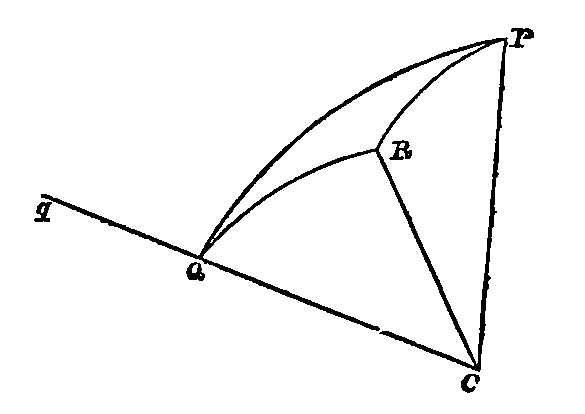
\includegraphics[width=0.5\textwidth]{332.png}
\centering
\end{figure}

Let \(C\) denote the centre of the spheroid, \(CP\) the semi-axis of
revolution, \(Q\) any point on the surface having for its polar coordinates
\(s\) and \(\theta\). Produce \(CQ\) to any point \(q\). It is required to
find the \textit{horizontal} attraction on a particle at \(q\). Let \(Cq = \delta\).
%%-----File: 333.png-----%%

Let \(R\) be any point on the surface having for its polar coordinates
\(s'\) and \(\theta'\). We suppose that the spheroid consists of a
sphere of radius \(s\) and an additional shell.

Let the angle \(PQR\) be denoted by \(\psi\), and the angle \(QCR\)
by \(\mu\).

The element of the shell at \(R = s^2 (s' - s) \sin \mu\,d\mu\,d\psi\).

The distance \(Rq = (s'^2 + \delta^2 - 2s'\delta \cos \mu)^{\frac{1}{2}}\).

The resolved attraction of the element in the plane \(RCq\) at
right angles to \(Cq\) is therefore
\[
\frac{s' \sin \mu s^2 (s' - s) \sin \mu\,d\mu\,d\psi}{(s'^2 + \delta^2 - 2s'\delta \cos\mu)^{\frac{3}{2}}}
\]
and resolving along the plane \(PCq\) we get
\[
\frac{s' \sin \mu \cos \psi s^2 (s' - s) \sin \mu\,d\mu\,d\psi}{(s'^2 + \delta^2 - 2s'\delta \cos \mu)^{\frac{3}{2}}}
\]

We have to integrate this between the limits \(0\) and \(\pi\) for \(\mu\),
and \(0\) and \(2\pi\) for \(\psi\); then we obtain the horizontal attraction
at \(q\) \textit{towards} \(P\).

We suppose with D'Alembert that \(s'\) has the value given in
Art.\ 425.

We shall obtain by effecting the integrations, neglecting the
square of \(\alpha\),
\[
\pi \alpha \sin \theta \left\{ \frac{4Br^4}{3\delta^3} + \frac{8Cr^5}{5\delta^4} \cos\theta + \frac{4Dr^4}{5\delta^3} - \frac{12Dr^6}{35\delta^5} + \frac{12Dr^6}{7\delta^5} \cos^2 \theta \right\}\text{.}
\]

In like manner if \(q\) be between \(C\) and \(Q\) instead of on \(CQ\)
produced, and \(Cq\) be called \(\delta\) as before, we obtain for the
horizontal attraction
\[
\pi \alpha \sin\theta \left\{ \frac{4Br^4}{3} + \frac{8C\delta}{5} \cos\theta + \frac{4Dr}{5} - \frac{12D\delta^2}{35r} + \frac{12D\delta^2}{7r} \cos^2 \theta \right\}\text{.}
\]

These expressions must be multiplied by a factor to represent
the density, if the density is not unity.

When \(\delta = r\) these expressions both coincide, as they should do,
with that given in Art.\ 425.
%%-----File: 334.png-----%%

\Section
438. The attraction at \(q\) in the direction at right angles to
the meridian plane of \(q\) will be zero, since the spheroid is supposed
a figure of revolution. D'Alembert himself makes the remark on
his page 216. He adds however that this can also be seen by
calculation; and he gives some calculations, which I do not find
to be intelligible.

\Section
439. In Art.\ 437 we have investigated expressions for the
horizontal attraction of the spheroid supposed homogeneous.
D'Alembert deduces on his page 218 the attraction of such a
spheroid on an included particle when the spheroid is composed of
indefinitely thin shells of varying density: the process is the same
as we have already found was used by Clairaut. See Arts.\ 323
and 336.

\Section
440. In order to obtain the whole action along the \textit{tangent} to
the meridian curve at any point, we must as in Art.\ 426 add to
the horizontal attraction the resolved part of the vertical attraction
along the tangent, and also the resolved part of the centrifugal
force.

\Section
441. Next we proceed to find the \textit{vertical} attraction on the
particle at \(q\).

Suppose the particle outside the spheroid. The vertical action
of the sphere of radius \(s\)
\[
= \frac{4\pi s^3}{3\delta^2} = \frac{4\pi r^3}{3\delta^2} (1+3\alpha A+3\alpha B\cos\theta+3\alpha C \cos^2\theta+3\alpha D \cos^3\theta)\text{.}
\]

We must now determine the vertical action of the shell. As
in Art.\ 437 we find that this is
\[
\int_{0}^{\pi} \int_{0}^{2\pi} \frac{(\delta-s' \cos\mu)s^2(s'-s)\sin\mu\,d\mu\,d\psi}{(s'^2+\delta^2 -2s' \delta \cos \mu)^{\frac{3}{2}}}\text{.}
\]

By effecting the integrations we obtain for the whole vertical
attraction
\begin{gather*}
\frac{4\pi r^3}{3\delta^2} (1+3\alpha A+\alpha C) - \frac{4\pi r^5\alpha C}{5\delta^4} +\pi\alpha \cos \theta \left\{\left(\frac{B}{3}+\frac{D}{5}\right)\frac{8r^4}{\delta^3} - \frac{48D r^6}{35\delta^5}\right\}\\
+ \pi\alpha \cos^2 \theta \frac{12Cr^5}{5\delta^4} + \pi\alpha \cos^3 \theta \frac{16Dr^6}{7\delta^5}\text{.}
\end{gather*}
%%-----File: 335.png-----%%

In like manner if the attracted particle be inside the spheroid,
the whole vertical attraction is
\begin{gather*}
\frac{4 \pi \delta}{3} + \frac{8 \pi \alpha C \delta}{15} + \pi \alpha \cos \theta \left\{- \frac{4Br}{3} - \frac{4Dr}{5} + \frac{36D \delta^2}{35r}\right\}\\
- \pi \alpha \cos^2 \theta \frac{8C \delta}{5} - \pi \alpha \cos^3 \theta \frac{12D\delta^2}{7r}\text{.}
\end{gather*}

For a point on the surface we must put in either of these
results \({\delta = r(1 + \alpha A + \alpha B \cos \theta + \alpha C \cos^2 \theta + \alpha D \cos^3 \theta)}\): it will be
found that each of them becomes then
\[
\frac{4 \pi r}{3} \left(1 + \alpha A + \frac{2 \alpha C}{5}\right) + \pi \alpha \cos \theta \frac{8Dr}{35} - \pi \alpha \cos^2 \theta \frac{4Cr}{15} - \pi \alpha \cos^3 \theta \frac{8Dr}{21}\text{.}
\]

These expressions must be multiplied by a factor to represent
the density, if the density is not unity. Then as in Art.\ 439 we
can obtain the vertical attraction for a spheroid composed of
indefinitely thin strata of varying density.

\Section
442. D'Alembert now discusses the relative equilibrium of
homogeneous fluid surrounding a solid nucleus composed of strata
of varying density: see his page 222. The problem is thus an
extension of that in Art.\ 426, and it is solved in the same manner.
There is no difficulty in the hydrostatical part of the problem; for
since the fluid is homogeneous it is sufficient for equilibrium that
the tangential action at every point of the surface should be zero.

If we equate to zero this tangential action, we obtain a result
of the form
\[
\sin \theta (M_{0} + M_{1} \cos \theta + M_{2} \cos^2 \theta) = 0,
\]
where \(M_{0}\), \(M_{1}\), and \(M_{2}\) are independent of \(\theta\). This leads, as in
Art.\ 426, to three equations
\[
M_{0} = 0, \quad M_{1} = 0, \quad M_{2} = 0\text{.}
\]

D'Alembert gives these three equations on his pages 222\dots 225.

\Section
443. We must be careful as to the notation, since many symbols
are required. D'Alembert leaves his notation to explain itself,
and it is not very inviting. I shall use the subscript \(1\) to denote
values relating to the external boundary of the fluid; and I shall
use \(\rho\) as a general symbol for the density. Then the three
%%-----File: 336.png-----%%
equations are
\begin{align*}
&\begin{multlined}
0 = \frac{4 \pi\alpha}{3 \delta^3} \int_{0}^{r_1} \rho \frac{d}{dr} (Br^4) dr + \frac{4 \pi \alpha}{35 \delta^5} \int_{0}^{r_1} \rho \frac{d}{dr} D(7r^4 \delta^2 - 3r^6) dr\\
- \frac{4 \pi \alpha B_1}{\delta^2} \int_{0}^{r_1} \rho r^2 dr,
\end{multlined}\\
&0 = \frac{8 \pi \alpha}{5 \delta^4} \int_{0}^{r_1} \rho \frac{d}{dr} (Cr^5) dr - \frac{8 \pi \alpha C_1}{\delta^2} \int_{0}^{r_1} \rho r^2 dr - \omega^2 r_1\\
&0 = \frac{12 \pi \alpha}{7 \delta^5} \int_{0}^{r_1} \rho \frac{d}{dr} (Dr^6) dr - \frac{12 \pi \alpha D_{1}}{\delta^2} \int_{0}^{r_1} \rho r^2 dr.
\end{align*}

These equations may be developed. I shall use the subscript \(0\)
to denote values relating to the internal boundary of the fluid.
Then between the limits \(r_0\) and \(r_1\) the density is constant, by
hypothesis; I shall denote it by \(\sigma\). Also for \(\delta\) we must put \(r_1\) to
the order which we wish to retain.

I will now express the second of the three equations in the
modified form which arises from the use of the notation just
explained; the other two equations may be similarly expressed.

In this equation \(\omega\) denotes the angular velocity; and I shall
put as usual \(j\) for \(\xp\dfrac{\omega^2 r_1}{\dfrac{4 \pi}{{r_1}^2} \displaystyle\int_{0}^{r_1} \rho r^2 dr}\). Thus we have
\begin{multline*}
\frac{2 \alpha \sigma}{ 5{r_1}^4} ({r_1}^5 C_1 - r_0^5 C_0) + \frac{2 \alpha}{5 {r_1}^4} \int_{0}^{r_0} \rho \frac{d}{dr} (Cr^5) dr\\
= \frac{2C_1 \alpha + j}{{r_1}^2} \left\{ \frac{\sigma}{3}({r_1}^3 - r_0^3) + \int_{0}^{r_1} \rho r^2 dr\right\}\text{.}
\end{multline*}

This equation corresponds with D'Alembert's on page 225;
he puts it so as to express \(\alpha\) in terms of the other quantities.
He takes \(r_1 = 1\) and \(C_1 = 1\), which he may do; but then by
mistake or misprint he \textit{also} takes \(C_0 = 1\), which he ought not
to do. This equation also exactly corresponds with equation (3) in
Art.\ 324; the \(\alpha C\) of the present Article is the \(- \epsilon\) of that Article.

\Section
444. D'Alembert passes on his page 225 to the problem in
which the entire spheroid is fluid, and is composed of indefinitely
thin strata of varying densities. He treats this problem according
%%-----File: 337.png-----%%
to his own peculiar views of hydrostatical principles. He arrives
at three general equations, each of which presents itself in a
\textit{primary} and in a \textit{derived} form, like Clairaut's equation of
Arts.\ 341 and 343.

D'Alembert's peculiar views lead him astray, and the consequence
is what we have already seen in Art.\ 405, namely, that
the results which he obtains are much more complicated than
they should have been.

For instance the third equation, with the notation of Art.\ 405,
is presented thus in its derived form by D'Alembert:
\[
\frac{d^2 D}{dr^2} + \frac{2\rho r^2}{\Upsilon(r)}\frac{dD}{dr} - \left\{\frac{12}{r^2} - \frac{2\rho r}{\Upsilon(r)}\right\}D = \frac{r^3 N}{\Upsilon(r)} \frac{d}{dr} \left\{\frac{1}{r^6} \frac{d}{dr} \left(\frac{\rho}{r} \frac{dr}{d\rho}\right)\right\},
\]
where \(N\) is a constant. But the correct form is that in which the
right-hand member is zero.

His second equation is precisely the same as (5) of Art.\ 405,
with \(C\) instead of \(\epsilon\); the error and the correction are the same as
we have already indicated in that Article.

In like manner the derived form of D'Alembert's first equation
is similarly embarrassed with a superfluous term. The \(K\) which
occurs on his page 231 should be zero. D'Alembert admitted his
errors in the fifth volume of his \textit{Opuscules Mathématiques}, page 5.

\Section
445. These differential equations for \(C\) and \(D\), when written
correctly with zero on the right-hand side, are cases of the general
equation, which Laplace's functions must satisfy, in Laplace's
Theory of the Figure of the Earth. This general equation is
\[
\frac{d^2Y_{i}}{dr^2} \frac{\Upsilon(r)}{r^i} + \frac{2\rho}{r^{i-2}} \frac{dY_{i}}{dr} + Y_{i} \left\{\frac{2\rho}{r^{i-1}} - \frac{i(i+1)\Upsilon(r)}{r^{i+2}}\right\} = 0\text{.}
\]

If we put \(2\) for \(i\) we arrive at the same differential equation for
\(Y_{2}\) as for D'Alembert's symbol \(C\); and if we put \(3\) for \(i\) we
arrive at the same differential equation for \(Y_{3}\) as for D'Alembert's
symbol \(D\).

Laplace shews that \(Y_{3}\) must be zero. If we put \(D = 0\) in the
differential equation for D'Alembert's symbol \(B\), we find that
this is the same as the above when \(1\) is put for \(i\).
%%-----File: 338.png-----%%

\Section
446. D'Alembert makes some remarks on the integration of
the differential equations which have been obtained; see his
pages 231\dots 234. By transformation he arrives at an equation
which he says is integrable in several cases; he gives three
cases: they are however unintelligible to me.

\Section
447. On his pages 234\dots 244 D'Alembert extends the calculation
of the horizontal and vertical attractions which we have
noticed in Arts.\ 437\dots 441: he introduces two new terms into the
expression for the radius vector of the attracting body, namely,
\(\alpha r (E \cos^4 \theta' + F \cos^5 \theta')\).

I have found on going over the calculation that there are
numerous misprints or errors in his results.

\Section
448. On his page 245 D'Alembert takes the case of a spheroid
composed of two fluids of different densities; he says that
the figures of the upper and lower strata must be determined by
the law of the perpendicularity of the action to each of the strata.
He adds:

\begin{squote}
Car dans le cas où les couches voisines different entr'elles sensiblement
par la densité, et ont une épaisseur finie, la pesanteur doit être
perpendiculaire à chacune. Voyez l'Appendice de mon \textit{Essai sur la résistance
des fluides.}
\end{squote}

The statement he makes here about the conditions of equilibrium
is true; but the reference to the \textit{Essai sur la résistance des
Fluides} is very remarkable: for the doctrine maintained in the
\textit{Essai} is precisely the reverse of that which is here affirmed in the
\textit{Recherches}. We read in the \textit{Essai} on page 206:

\begin{squote}
Supposons maintenant que le Fluide soit composé de plusieurs couches
différemment denses, et dont la différence de densités soit finie; je dis
que le Fluide pourra encore être en équilibre, quoique les surfaces qui
séparent ces différentes couches ne soient point de niveau\dots.
\end{squote}

Suppose \(p\) the pressure at any point of the surface bounding
fluids of different densities. Let \(S\) be the force, if any, resolved
along a tangent to the surface. Then proceeding along an element
of this tangent we should have in one fluid \(dp = \rho Sds\), and in the
other fluid \(dp = \rho'Sds\), where \(\rho\) and \(\rho'\) are unequal. But these
values of \(dp\) must be equal; therefore \(S\) must \(= 0\).
%%-----File: 339.png-----%%

This assumes that there is no discontinuity in the forces
acting at the common surface. In the remarks on page 206,
D'Alembert's \textit{Essai}, which follow and support the words we have
quoted, he allows a discontinuity to occur in the forces.

\Section
449. D'Alembert's fifth Chapter, on pages 247\dots 260 is entitled
\textit{De l'attraction d'un sphéroïde qui n'est pas un solide de
révolution.} This Chapter is not important; it merely indicates
how we ought to proceed, and shews that in some cases the integrations
could be effected.

\Section
450. On his page 256 he makes a mistake to which I have
drawn attention in Art.\ 381. He says:

\begin{squote}
J'ai fait voir, par exemple, dans mes \textit{Recherches sur la cause des vents}
art.\ 84.\ n\textsuperscript{o}.\ 10.\ qu'un sphéroïde elliptique, homogene et fluide, tournant
autour de son axe, ne pouvoit subsister, si les méridiens n'étoient pas
tous égaux et semblables;\dots
\end{squote}

\Section
451. On his page 258 he alludes to the case in which we
require the attraction, not of a whole spheroid, but of a segment
of a spheroid. Then on his page 259 he takes for special consideration
the case of a semi-spheroid; but his first paragraph is
unintelligible to me: in his second paragraph he asserts that the
attraction along the radius of a semi-spheroid is half the attraction
of the whole spheroid, which, however, is not necessarily true of
\textit{any} semi-spheroid, though it would be true if the whole spheroid
were cut \textit{symmetrically} into two halves.

\Section
452. Let us now appreciate the contributions to our subject
which D'Alembert made in his \textit{Recherches \dots\ Systême du Monde.}

The method of estimating the attraction of a spheroid by resolving
the body into a sphere and a thin additional shell, which is
here systematically employed, is very valuable.

Assuming that the radius vector of a spheroid is
\[r + \alpha r (A + B \cos \theta' + C \cos^2 \theta' + D \cos^3 \theta' + E \cos^4 \theta' + F \cos^5 \theta')\]
where \(\alpha\) is very small, he gives expressions for the resolved attractions
on any particle, external or internal, the spheroid being
either homogeneous or composed of indefinitely thin strata of
%%-----File: 340.png-----%%
varying density. The calculations are laborious; and though
D'Alembert's results are not free from error, yet they furnish
useful information.

Retaining the terms in the radius vector as far as \(D \cos^3 \theta'\)
inclusive, D'Alembert gave the equations which must be satisfied
by \(B\), \(C\), \(D\), supposed variable, to ensure the relative equilibrium
of a fluid mass. His equations are encumbered with terms which
are really non-existent; but still in their derived forms the remarkable
similarity between them to which we have drawn attention
in Art.\ 445 is made apparent. I consider it to be quite
possible that this similarity may have struck the attention of
Legendre and Laplace, and thus contributed to the construction
of the general equation.

As I have already hinted, D'Alembert himself over estimated
the value of the conclusions that he drew from his peculiar views
of Hydrostatics. In the preface to the third volume of these
\textit{Recherches \dots\ Systême du Monde}, page xxxvi, he states that
hitherto the Theory of the Figure of the Earth had been restricted
to verifying the agreement of the elliptic figure with the
laws of Hydrostatics; and then adds, ``j'ai trouvé de plus, et je le
démontre dans cet Ouvrage, qu'il y a une infinité d'autres figures
qui s'accordent avec ces loix, surtout si on ne suppose pas la Terre
entierement homogene.'' This, however, as we now know is
unsatisfactory. For instance, D'Alembert indeed arrives at an
equation which his symbol \(D\) must satisfy, as we saw in Art.\ 444;
but he does not solve the equation, and so shew that \(D\) is a real
quantity: on the contrary, Laplace, in fact, shews that \(D\) must
be zero.
%%-----File: 341.png-----%%
\Chapter{CHAPTER XIV.}
\Subhead{BOSCOVICH AND STAY.}
\Runhead{\textsc{boscovich.}}

\Section
453. \textsc{The} present Chapter will contain an account of the
contributions made by Boscovich to our subject, together with a
notice of the poem by Stay to which Boscovich added copious
explanations.

\Section
454. In 1750 two Jesuits, Maire and Boscovich, began to
measure an arc of the meridian in the Papal States. The account
of the survey appeared at Rome in 1755, under the title \textit{De
Litteraria Expeditione per Pontificiam Ditionem}. The volume is
in quarto; it consists of Title, Dedication, Preface, and Index in
xxii pages, and the text in 516 pages: there are three pages of
Errata, and four Plates. A French translation was published at
Paris in 1770.

The dedication is to Benedict XIV., by whose command the
survey was executed: behind the cloud of incense raised by the
authors, we may discern the figure of a sagacious and enlightened
Pontiff.

\Section
455. The book is divided into five parts. The first gives the
history of the proceedings, the second the calculations for the
determination of the length of a degree of the meridian, the third
the correction of the map of the district, the fourth an account of
the instruments employed, the fifth a treatise on the Figure of the
Earth. The second and third parts are by Maire; the others are
by Boscovich.

I shall not enter into any examination of the practical operations
recorded in the volume; they have been criticised by
%%-----File: 342.png-----%%
De Zach in his \textit{Correspondance Astronomique}, Vol.\ \textsc{vl}: see however,
Airy's Article on the \textit{Figure of the Earth}, in the \textit{Encyclopædia
Metropolitana}, page 207.

\Section
456. The fifth part of the book is that which we have to
examine, This occupies pages 385\dots 516, and is entitled \textit{De
Figura Telluris determinanda ex æquilibrio, et ex mensura graduum}.
After a few introductory sentences, the treatise is divided
into two Chapters: the first, extending to page 481, relates to the
Figure of the Earth, as deduced from the theory of fluid equilibrium;
the second relates to the Figure of the Earth as determined
by the measure of degrees.

\Section
457. It must be observed that before the publication of the
book, Boscovich had issued various dissertations, bearing more or
less on our subject: these seem to have been academical exercises
which he delivered in his character of professor at the
Roman College. I have not seen any of these dissertations.
Boscovich refers to them generally on pages xviii and 386 of
the book: from the latter page it appears that few copies of the
exercises were printed, and of these the larger part perished.
Probably the treatise reproduces all that was valuable with respect
to our subject in the previous publications. The dates
and titles of some of these dissertations are given in the pages of
the work which I have recorded after them:

1738. De Telluris figura, 23.

1739. De figura Telluris, 395, 399, 445, 447, 487. Perhaps
we may infer from the last three lines on page 445, that this was
reprinted in a subsequent year.

1741. De Inæqualitate Gravitatis, 23.

1742. De Observationibus Astronomicis, 23, 475.

1748. De Maris Æstu, 390.

De Lege virium in natura existentium, 416. The date is not
stated, but it is said \textit{exposui nuper}.

I give the titles as I find them: it is possible however, that
there may be only \textit{one} dissertation instead of the two which appear
dated 1738 and 1739.
%%-----File: 343.png-----%%

\Section
458. The work of Boscovich, to which we now proceed, may
be described in general as out of date, even when first published:
it is chiefly written in an antiquated geometrical fashion, which
one would have thought little likely to be adopted for this subject
after the appearance of Clairaut's treatise. The Latin seems to
me much more elaborate than is usual in the scientific literature
of the period: this might perhaps have been expected from
an Italian and a Jesuit.

\Section
459. Up to his page 417, Boscovich considers the case of homogeneous
fluid attracted to a fixed point by a force which is any
function of the distance, and rotating with uniform angular velocity
round an axis through the fixed point: the analytical solution
of this problem is very short and simple, as we have seen in
Art.\ 56. Boscovich gives correct but tedious geometrical constructions,
and devotes special attention to two cases, namely, that
in which the force is constant, and that in which it varies as the
distance: in this way he contrives to fill thirty pages.

Boscovich gives on his page 399 a good elementary investigation
like that on Clairaut's page 143: see Art.\ 297.

\Section
460. A strange mistake occurs on pages 411 and 412. Boscovich
has assumed a value for the radius of the equator, and has
found as usual that the ratio of the centrifugal force at the equator
to the attraction there, is that of 1 to 289. He adds:

\begin{squote}
\dots\ Si gradus æquatoris fuerit major, vel minor, in eadem ratione
duplicata major, vel minor erit sinus versus arcus similis, adeoque et vis
centrifuga, et proinde in eadem ratione duplicata minuendus erit
posterior proportionis numerus.
\end{squote}

But the word \textit{duplicata} ought to be omitted: moreover, corresponding
to the words \textit{vel minor}, the words \textit{vel augendus} should
be inserted after \textit{minuendus}.

\Section
461. On his page 417, Boscovich says that he will investigate
the Figure of the Earth on the Newtonian hypothesis of gravity,
and will illustrate in the first place Maclaurin's solution: Boscovich
refers to Maclaurin's \textit{Prize Essay on the Tides}, and not to the
more complete investigations contained in the \textit{Fluxions}.
%%-----File: 344.png-----%%

Thus from page 417 to page 448, Boscovich may be said to
reproduce in substance Maclaurin's discussion of the relative
equilibrium of a mass of homogeneous rotating fluid. We shall
only have to notice a few matters which present some novelty.

\Section
462. Boscovich begins with a demonstration of a theorem
in Conic Sections which forms the fourth Corollary to the first
Lemma in Maclaurin's Essay. Boscovich considers his own
demonstration, which is geometrical, more simple and more elegant
than an analytical demonstration, which he ascribes to
Calandrinus, printed in what we call the Jesuits' edition of the
\textit{Principia}. Boscovich does not remark that Clairaut had already
given a very good demonstration by the method of projections:
see Clairaut's page 159.

\Section
463. On his page 424, Boscovich enunciates the following
theorem:

\begin{squote}
Si in massa quadam fluida particulæ omnes ejusmodi viribus animatæ
sint, ut assumpto intra eam puncto quocumque, bini quicumque canales
rectilinei ducti inde ad superficiem extimam in æquilibrio sint, ea massa
erit in æquilibrio.
\end{squote}

In his demonstration he shews that if at every point rectilinear
columns are in equilibrium, so also are curvilinear canals of every
form, and that a particle at the surface has no tendency to move.
The part relating to curvilinear canals is the most interesting:
this, however, had already been formally treated by D'Alembert
in his \textit{Essai sur la Résistance des Fluides}, page 15.

On his page 432, Boscovich supplies in fact a demonstration of
what Maclaurin contented himself with affirming in the words ``in
like manner it is shewn'': see Art.\ 245.

\Section
464. Boscovich has to compare the attractions of an oblatum
on a particle at the pole and at the equator respectively. After
remarking on page 435, that Newton had shewn how to calculate
the attraction at the pole, Boscovich adds:

\begin{squote}
\dots\ sed pro puncto posito in æquatore rem nequaquam perfecit,
verum crassa quadam æstimatione invenit utcumque pro ellipsoide data,
%%-----File: 345.png-----%%
et parum abludente a sphæra. Mac-Lavrinus multo sane elegantius
accuratissime, et felicissime rem perfecit tam pro puncto posito in polo,
quam pro puncto posito in æquatore;\dots
\end{squote}

However, Boscovich says that he will himself adopt a method
which is nearly the same as Bernoulli's; it is the method, really
due to Clairaut, which we have noticed in Arts.\ 165 and 233.
Boscovich professes to use Geometry alone: but the Geometry
consists chiefly in denoting the length of every straight line by
two capital letters instead of a single small letter: this strange
notion of Geometry has survived to our own times in the University
of Cambridge.

\Section
465. Boscovich arrives at the usual result for the attraction
of the excess of an oblatum over the inscribed sphere, on a particle
at the pole; and with some enthusiasm he says on his page 438,
Et ea quidem est elegantissima, et simplicissima expressio ejus vis.

From this result he deduces very briefly and easily the attraction
of the excess of a sphere over the inscribed oblatum on a
particle at the equator: see his page 439.

Hence finally he arrives at the equation which we have frequently
given in our notation; namely \(\epsilon = \xp\dfrac{5j}{4}\): see his page 441.

\Section
466. A digression on pages 442\dots 447 is devoted by Boscovich
to Hermann. I have already noticed Hermann's \textit{Phoronomia}, and
I presume this is the work Boscovich has in view; but it does not
seem so obvious to me as to Boscovich, that Hermann held Newton
and David Gregory to be wrong: see Art.\ 95. Boscovich says
on his page 442:

\begin{squote}
Et quidem Hermannus censuit, hanc ipsam suam Ellipsim esse illam,
quæ in Newtoniana gravitatis theoria debeat obvenire, ac Gregorium, et
Newtonum ipsum culpandos existimavit, quod ii id ipsum non viderint,
et plusquam duplo majorem justo compressionem Telluri tribuerint,
quam ipsa illorum principia postularent. At Hermannus ipse in eo
erravit sane quamplurimum,\dots
\end{squote}

The \textit{ipsum} after \textit{Newtonum} marks Boscovich's opinion of Hermann's
audacity.
%%-----File: 346.png-----%%

The digression is interesting because Boscovich allows that he
was himself for a time to some extent misled by Hermann. Boscovich
in 1739 was thus induced to suspect that the oblatum,
which Newton had assumed without demonstration, was not a
possible form for relative equilibrium; but in the following year
Maclaurin's demonstration settled the matter, and then Boscovich
was led to investigate the cause of Hermann's error: accordingly
he points out what he considers to be the \textit{erroris primus fons}, and
the \textit{alter ejusdem erroris fons}.

It may be doubted whether Boscovich himself was quite clear
on the subject; he appears to fall into the mistake which has been
pointed out in Art.\ 33, for he does not introduce the important
condition involved in the words \textit{resolved along the radius}: see his
page 443. But in his commentary on Stay's poem, at a rather
later date, he is quite correct: see his Article 244 on pages 371
and 372 of Vol.\ \textsc{ii}.

\Section
467. On his page 448, Boscovich gives an elegant investigation
of the diminution of gravity in passing from the pole to the
equator. But by gravity he really means gravity resolved \textit{along
the radius}, which is not strictly the same as the gravity which is
measured by observations: see Art.\ 34.

\Section
468. Boscovich now proceeds to consider the Figure of the
Earth when it is not supposed to be homogeneous. He assumes
that there is a spherical homogeneous nucleus surrounded by fluid
which is also homogeneous, but not of the same density as the
nucleus: to this discussion he devotes his pages 448\dots 457. The
investigation is tedious, but was probably considered by the author
to be a choice specimen of his geometrical methods. Although
the whole discussion was quite superfluous after the publication of
Clairaut's treatise, yet there is one matter of principle in which
Boscovich is rather superior to Maclaurin. As we have already
stated, when Maclaurin supposed the earth to be fluid, but not
homogeneous, he did not demonstrate that the whole mass would
be in equilibrium; see Arts.\ 264, 267, 269. Boscovich shews by
his language that he saw this difficulty; he says on his page 458:
%%-----File: 347.png-----%%

\begin{squote}
\dots\ Idcirco ego, ut methodum canalium tuto adhiberem, massam
solidam prius ad homogeneitatem adduxi, amandata in centrum redundante
materia, tum dissolvi.
\end{squote}

We will give a notion of Boscovich's method. Suppose we
have to consider the case in which there is a homogeneous fluid
surrounding a solid spherical nucleus; and let the density in the
nucleus be a function of the distance from the centre. Reduce
the density of the nucleus to that of the fluid, and put a force at
the centre, producing an attraction equal to that of the excess of
the solid nucleus above an equal volume of fluid. Then suppose
the nucleus to become fluid. If the additional force at the centre
attracted as the distance from the centre, we should thus obtain a
problem which has been fully discussed by Maclaurin; for he has
considered forces varying as the distance from the axis and from
the plane of the equator, besides the attraction of the fluid: see
Art.\ 245. Boscovich then by a supplementary investigation has to
allow for the difference between his supposed force at the centre
which attracts as the distance, and the real force which would
attract inversely as the square of the distance.

\Section
469. Boscovich obtains a result which, as he says, had
previously been given by D'Alembert and Clairaut: see Art.\ 377.

Boscovich points out that the result differs from one which
Daniel Bernoulli had given in his Essay on the Tides, and which
had been criticised by D'Alembert. I do not stay to discuss the
point, as it does not strictly belong to our subject but to that of
the Tides. See D'Alembert's \textit{Réflexions sur \dots\ des Vents}, page 56;
Laplace's \textit{Mécanique Céleste}, Vol.\ \textsc{v}.\ page 150; and page 8 of
Lubbock's work mentioned in Art.\ 233.

It may however be observed that Boscovich seems to have
supposed that D. Bernoulli's result ought to have coincided with
his own, although the circumstances of the problems differ in a
very important respect. In D. Bernoulli's problem the fluid is
exposed to the attraction of a distant body, and this attraction,
does not reduce to a single force tending to the centre and
varying as the distance, which is the case that Boscovich considers.
%%-----File: 348.png-----%%

\Section
470. In his pages 459\dots 465 Boscovich discusses the result
which, as we have stated in Art.\ 469, he had obtained in agreement
with D'Alembert and Clairaut. Boscovich shews that in
certain cases the external surface is an oblongum, not an oblatum;
it appears however from his page 463, that he held the oblongum
to be in modern language an \textit{unstable} form. See Art.\ 378.

\Section
471. In his pages 466\dots 468, Boscovich demonstrates \textit{Clairaut's
Theorem}, on the same hypotheses as to the constitution of the
Earth which had been used to obtain the result of Art.\ 469. He
draws some inferences from the theorem in his pages 469\dots 471.

\Section
472. Boscovich now proceeds to the subject of the variation
of gravity as tested by experiments with the pendulum. He suggests
local inequalities as the cause of the observed irregularities.
He calculates the effect which would be produced on the plumb-line
by the attraction of a sphere of the mean density of the Earth,
of a geographical mile in radius, for various positions of the sphere;
see his pages 472\dots 474.

One of his results is that such a sphere as we have mentioned,
if placed just beneath the surface of the Earth in addition to the
matter already there, would increase the length of the pendulum
by one-eighth of a line. Then he says that if for the depth of
eight geographical miles the density at the pole is twice that at
the equator the length of the pendulum at the pole will be a line
longer. This, he says, follows from what has been demonstrated:
but there seems to be some mistake. If \(r\) be the radius, and \(\rho\)
the density, of a sphere, the attraction at the surface is \(\xp\dfrac{4\pi\rho r}{3}\).
Now if the density at the pole is changed from \(\rho\) to \(2\rho\) throughout
the depth \(h\), the additional result is approximately the same as
would be produced by the attraction of an infinite plate of thickness
\(h\): and so it is \(2\pi\rho h\). Suppose \(h = 8r\); then the result becomes
\hypertarget{472:1}{\(16\pi\rho r\)}: this is \textit{twelve} times the former result \(\xp\dfrac{4\pi\rho r}{3}\). Accordingly
instead of an increase of \textit{one} line in the length of the
pendulum we obtain an increase of \(\xp\dfrac{12}{8}\) of a line, that is, of a line
and a half.
%%-----File: 349.png-----%%

\Section
473. Boscovich refers to the curious opinion expressed by
Newton to which we drew attention in Art.\ 31; Boscovich says on
his page 475:

\begin{squote}
Newtonus censuit prope æquatorem debere densitatem esse potius
majorem in partibus nimirum a Sole quodammodo veluti tostis. Ego
contra, cum tam multa corpora dilatentur caloris vi, et vi frigoris
adstringantur, opinor debere potius rariora ibi esse corpora ob id ipsum.
Sed externi caloris, et frigoris vis ad tantam altitudinem infra superficiem
non pertingit, ut effectum sensibilem edat in partem utramlibet.
\end{squote}

\Section
474. Boscovich notices the fact that according to observations
made by Bouguer and La Condamine, the attraction of a large
mountain in Peru was much less than it ought to have been,
supposing its density equal to the mean density of the Earth: see
Art.\ 363. Boscovich offers a conjecture in explanation of this
fact; he says on his page 475:

\begin{squote}
\dots\ Verum montes quidem plerique, ut ego arbitror, effecti sunt
intumescentibus interni caloris vi stratis superficiei proximis; quod
quidem si ita contigit, nihil ibi materiæ accedit, et vacuus inter viscera
hiatus compensat omnem illam apparentem materiæ in montem assurgentis
congeriem.
\end{squote}

\Section
475. Boscovich observes that a greater effect might be produced
on the pendulum by a large tract of raised land than by a
single mountain. He refers to a problem on this point which he
had given in his dissertation \textit{De Observationibus Astronomicis}, 1742.
The problem is the following: cut a slice from a sphere by two
parallel planes, one passing through the centre; bisect the slice
by a plane perpendicular to the circular ends: then find the
attraction, resolved parallel to the planes of the circular ends,
of one of the halves on a particle situated at that point
of the half which was originally the centre of the sphere.
Boscovich states, without investigation, an approximate result for
the case in which the thickness of the slice is very small compared
with the radius of the sphere: but this result is incorrect. In his
commentary on Stay's poem, Vol.\ \textsc{ii}., page 382, he gives a correct
investigation. If we wish to confine ourselves to the order of
approximation which is sufficient for his numerical application, we
may replace the slice of a sphere by the slice of a cylinder. Let \(a\)
%%-----File: 350.png-----%%
be the radius of the slice of the cylinder, \(h\) the thickness, \(\rho\) the
density. Then the required result is easily found to be
\[2\rho h\int_{0}^{a}{\frac{dr}{\xsurd(r^2 + h^2)}},\]
that is
\[2\rho h \log {\frac{a + \xsurd(a^2 + h^2)}{h}}.\]

If we suppose \(h\) very small compared with \(a\), we get approximately
\(2\rho h \log \xp\dfrac{2a}{h}\), that is \(\xp\rho h \left(2 \log \dfrac{a}{h} + 2 \log 2\right)\); this agrees closely with
\(\xp\rho h\left(2 log \dfrac{a}{h} +1·389\right)\), which is Boscovich's result in his Commentary
on Stay's poem.

\Section
476. Boscovich makes a curious suggestion on his page 477.
He proposes to have a pendulum in a tower by the sea shore, at
some place in England or the opposite continent, where the water
may be raised by the high tide 50 feet above the level of the low
tide. He considers that if the density of the sea is equal to the
mean density of the Earth, a deviation of about \(2''\) will be
produced in the direction of the pendulum. By having a long
pendulum and using a microscope, he thinks the deviation might
be observed, and thus some notion obtained of the mean density
of the Earth. See some remarks on this suggestion in De Zach's
work, \textit{L'attraction des montagnes}, page 17.

\Section
477. In his pages 477\dots 481, Boscovich cites some observations
of pendulums, and draws inferences from them: he had
recently made some observations at Rome, in conjunction with
La Condamine, with the pendulum which had been used in
America and at the Cape of Good Hope.

\Section
478. We now reach the second Chapter of Boscovich's treatise;
this relates to the Figure of the Earth, as determined by the
measure of degrees.

He begins with some general explanation as to what is meant by
a degree, and an osculating circle; see his pages 481\dots 486: these
present nothing of interest except a curious mistake. Let \(s\) denote
an arc of a curve measured from some fixed point, \(\rho\) the radius of
curvature at the variable extremity of the arc, and \(\phi\) the inclination
%%-----File: 351.png-----%%
of \(\rho\) to a fixed straight line: then we know that \(\xp\dfrac{ds}{d\phi} = \rho\). By
the length of a degree, we mean the value of \(\displaystyle\int\rho d\phi\) taken between
limits which differ by the circular measure of a degree. Thus the
length must be equal to \(\rho_{1}\xp\dfrac{\pi}{180}\), where \(\rho_{1}\) is some value of \(\rho\) which
lies between the least and the greatest of the values which
occur within the range of integration, \(\rho\) being supposed always
finite. This statement follows from the first principles of the
Integral Calculus; Boscovich, however, denies the universal truth
of it, for he says on his page 484:

\begin{squote}
\dots\ Fieri itidem potest, ut arcus unius gradus plurimum differat a
gradu circuli osculantis curvam ubique intra cum arcum, quod quidem
tum accidere potest, cum curvatura pergendo ab altero ejus extremo ad
alterum primo quidem perpetuo crescit, tum perpetuo decrescit, vel
vice versa.
\end{squote}

\Section
479. On his page 487, Boscovich seems to adopt a definition
which has not been used by others. If \(2a\) and \(2b\) are the major
and minor axes respectively of an ellipse, we call \(\xp\dfrac{2b^2}{a}\) the latus
rectum: Boscovich seems to call \(\xp\dfrac{2b^2}{a}\) the latus rectum with respect
to the major axis, and \(\xp\dfrac{2a^2}{b}\) the latus rectum with respect to the
minor axis.

In his pages 487\dots 493, Boscovich gives various geometrical
constructions relating to the ellipse and its radius of curvature;
he says on page 488:

\begin{squote}
Exhibebo autem solutiones diversas ab iis, quas simplicissimas sane, et
admodum elegantes, ac geometricas itidem exhibui in mea dissertatione
illa de Figura Telluris.
\end{squote}

Thus he seems to have been very well pleased with some of
his own work; for I presume we are to consider the demonstrations
in the book at least as good as those which had appeared in
the dissertation.
%%-----File: 352.png-----%%

A property of the ellipse may be noticed which he demonstrates
on his page 489. The normal at any point \(P\) of an ellipse meets
the minor axis at \(G\); from \(P\) a perpendicular \(PM\) is drawn to the
minor axis meeting at \(Q\) the circle which is described on the
minor axis as diameter; from \(G\) a straight line is drawn parallel
to \(CQ\), meeting \(MP\) produced at \(N\); then \(GN\) is equal to half
the latus rectum \textit{with respect to the minor axis}, and \(MP\) is a
mean proportional between \(MQ\) and \(MN\).

\Section
480. Boscovich obtains on his page 494 an approximate
formula, which determines the ellipticity of the Earth from the
lengths of a degree of the meridian at the pole and the equator;
Boscovich refers to Maupertuis, who had previously obtained the
formula: see Maupertuis's \textit{Figure de la Terre \dots} page 130.

Boscovich however considers that the exact theorem is more
elegant, namely, that the lengths of a degree of the meridian at
the equator and the pole are respectively as the inverse cubes of
the corresponding diameters.

Boscovich shews on his pages 495 and 496 that the diminution
of the length of a degree of the meridian from the pole to the
equator varies as the square of the cosine of the latitude: hence
the ellipticity may be found by measuring arcs of the meridian.

\Section
481. Boscovich now proceeds to consider the actual measures
of a degree of the meridian in various places. He says that there
are only five measures which are accurate; namely, those in
France, in Lapland, in Peru, at the Cape of Good Hope, and his
own in the Papal States: see his page 497.

He holds that the value of Picard's degree may now be considered
perfectly settled \textit{post mutationes quatuor}. It is not certain
what is meant by \textit{four changes}; in Art.\ 236, \textit{four} different values
are given, and these are also recorded by Boscovich himself in his
commentary on Stay's poem, Vol.\ \textsc{ii}., page 392. But if there
were four changes, there must have been five different values:
perhaps then we are to include a result obtained by J. Cassini,
which was between 30 and 50 toises less than Picard's own: see
\textit{De la Grandeur et de la Figure de la Terre}, page 286.
%%-----File: 353.png-----%%

Boscovich alludes to Norwood's measure, and gives a few
lines to Snell's measure; he considers them both unsatisfactory:
see Arts.\ 68 and 105.

\Section
482. Boscovich on his pages 499\dots 503 deduces the ellipticity
of the Earth by ten different binary combinations of the
five arcs; but he finds that the results are very discordant. One
combination actually brings out a negative ellipticity; namely, the
combination of the Roman arc with the African. The other combinations
give various values of the ellipticity, the greatest
being \(\xp\dfrac{1}{128}\), and the least about one-tenth of this. The mean
ellipticity is \(\xp\dfrac{1}{255}\); but if the two combinations be rejected which
differ very much from the rest, the mean ellipticity is \(\xp\dfrac{1}{195}\).

Boscovich has some troublesome misprints on his page 501;
the ellipticities deduced from his sixth and tenth combinations are
quite wrong: and the numbers which he gives in his following
Article to denote the mean excesses of the polar degree above the
equatorial are a third of the true values.

\Section
483. Boscovich says on his page 501 that some persons had
tried to conciliate the results by forcing the observations:

\begin{squote}
Nonnulli, ut nuperrime Eulerus in schediasmate, cujus summam
quandam mihi humanissimè communicavit hìc Romæ præsens, dum hæc
scribo, Condaminius, observationibus vim inferunt, ut omnia concilient.
Et is quidem gradum Lapponiensem, Africanum, Quitensem, mutatione
adhibita hexapedarum 19 in singulis, conciliat cum ellipsi Newtoniana,
sed Gallicus Piccardi gradus corrigendus illi est hexapedis 169, quem
idcirco sibi maximè suspectum esse profitetur, et novas in Gallia mensuras
desiderat. At id quidem errorem exposcit intolerabilem sane in
gradu cum ingenti cura definito a peritissimis viris.
\end{squote}

It seems absurd to suppose that an error extravagantly the
greatest should occur in the arc which must have been the best
determined of all at the epoch. We shall recur to Euler's speculations
in Chapter XV.
%%-----File: 354.png-----%%

\Section
484. On his pages 502\dots 506, Boscovich discusses Bouguer's
hypothesis that the increment of the length of a degree of the
meridian in proceeding from the equator to the pole varies as the
fourth power of the sine of the latitude: see Art.\ 363. Boscovich
considers that the African arc overturned this hypothesis. But
then it should be observed that the African arc presented much
difficulty when compared with the others.

Boscovich observes in a despairing tone: ``Quocumque te
vertas, nihil certum, sibi constans, et regulare occurrit.''

He gives on his pages 507\dots 510 reflections on the state of
knowledge of the subject: he sums up his opinions vigorously on
his page 508 as to what had been established. Instead of the
inquiry respecting the Figure of the Earth from the measures of
degrees being finished, he considers that it had scarcely been
commenced. Still some valuable results had been obtained: the
hypothesis of an attraction directed to a fixed point was excluded,
and the compression at the poles was extremely probable, though
the amount of this compression was uncertain.

\Section
485. On his page 510, Boscovich says that the observations
were not inconsistent with the hypothesis of a nucleus in which
the density, in modern language, is a function of the distance from
the centre. He makes two statements, as to what Clairaut had
established, which seem not strictly accurate.

One statement is this: assuming that Clairaut's fraction is
greater than \(\xp\dfrac{5j}{4}\), \textit{then the density of the nucleus must be greater
than the mean density of the Earth}, but the ellipticity less than
\(\xp\dfrac{5j}{4}\). If Clairaut's fraction is greater than \(\xp\dfrac{5j}{4}\), the ellipticity must
be less than \(\xp\dfrac{5j}{4}\), by Art.\ 336. But the statement that the density
of the nucleus \textit{must be greater} than the mean density of the
Earth does not seem justified by anything in Clairaut: the
nearest approach to it is in the second criticism of Art.\ 325, but
this obviously falls short of the statement.
%%-----File: 355.png-----%%

Again Boscovich proceeds thus:

\begin{squote}
\dots\ Invenit autem ejusmodi fractionem majorem revera esse, et
affirmavit ellipticitatem \textit{minorem} erui e graduum mensura; unde intulit,
ea duo conciliari non posse, nisi assumatur certa nuclei ipsius ellipticitas.
\end{squote}

The word \textit{minorem}, which I have put in Italics, must be a
misprint for \textit{majorem}; see Art.\ 349. Then for all that follows
\textit{intulit} there seems not sufficient authority; the criticism in the
first paragraph of Art.\ 325 is somewhat short of this.

\Section
486. Boscovich considers that more observations of pendulums
and more measurements of degrees are required; he admits
that this would involve great labour and expense, but he adds,
``at nihil est, quod Astronomorum patientia, et munificentia
Regum superare non possit:'' see his pages 511 and 512. Since
his time the endurance of Astronomers and the liberality of
Sovereigns have been largely exercised in the subject.

He repeats on his page 513 that the fact of the compression at
the poles might be admitted; but the amount of the compression,
and the true Figure of the Earth, were still quite uncertain.

He finishes by giving on his pages 514\dots 516 approximate
solutions of the problem to determine the Figure of the Earth,
assumed to be an oblatum, from two measured degrees, one or
both of which might be of longitude.

\Section
487. In forming an estimate of the treatise we must remember
that the author had prescribed to himself the condition of
supplying \textit{geometrical} investigations; so the Differential Calculus
was not to be introduced. We must consider the treatise rather
as the work of a professor for the purposes of instruction, than of
an investigator for the advancement of science; and then we may
award the praise that the task proposed is fairly accomplished.
It would have been more desirable to study Clairaut's work than
to be confined to Boscovich's geometrical methods: but the experience
of our own university shews us that it is possible to find
the methods used for teaching occasionally some years in arrear of
those used for investigation.

Although the mathematical processes seem a little out of date,
yet Boscovich's treatise reveals, I think, great knowledge and
judgment in Natural Philosophy.
%%-----File: 356.png-----%%

\Section
488. Boscovich has an unpleasant habit of giving hints as
to matters which will be found in other parts of his book, without
supplying exact references; I have observed many passages of this
kind, and have not always been able to determine with certainty
to what he is pointing. Thus we have on page 392, ``de qua
fortasse aliquid alibi infra;'' on page 413, ``videbimus;'' on
page 448, ``porro videbimus;'' on page 455, ``ut infra patebit;''
on page 466, ``ut infra videbimus;'' on page 506, ``ut vidimus;''
on page 507, ``ut innui etiam;'' on page 508, ``supra innui.''
None of these allusions, however, are to matters of great importance;
but there is a passage of more interest on page 386:

\begin{squote}
\dots\ Expediam autem, quod ad eam gravitatis legem pertinet, sive
Tellus homogenea sit, in quo argumento felicissime sane Mac Laurinus
se gessit, sive diversam in diversis distantiis densitatem habeat, de quo
casu multo aliter ego quidem sentio, quam summi etiam nostræ ætatis
viri senserint, quorum calculos laborare omnino censeo, cum Geometria
duce ad conclusiones delabar prorsus contrarias eorum conclusionibus.
\end{squote}

I cannot see anything in the treatise which corresponds to
``de quo \dots\ conclusionibus.'' Boscovich seems to dissent from only
one person, namely Daniel Bernoulli, and D'Alembert had previously
objected to the same thing: see Art.\ 469.

\Section
489. Boscovich himself gave an abstract of his treatise in
the Bologna \textit{Commentarii}, Vol.\ \textsc{iv}.\ 1757, pages 353\dots 396. This
supplies nothing of importance to our subject except three separate
sentences, which I quote, because I do not understand them.

With reference to the arc in Lapland, Boscovich says on
page 389:

\begin{squote}
\dots\ et in Lapponia, adhibita huic postremo illa correctione, quæ
adhibita est etiam a Bouguerio, et præter quam alias adhibendas non esse,
ut ut ab alio nuper adhibitas, demonstrari facile potest.
\end{squote}

Bouguer's correction is that for refraction; I do not know what
the other corrections are, nor by whom they were proposed.

After drawing an inference from Clairaut's theorem, Boscovich
says on page 392:

\begin{squote}
\dots\ quod ipsum cum ego in eo opusculo diserte affirmaverim, et
Clerautii theorema ipsum ex mea theoria deduxerim, ipso Clerautio
nominato, miratus sane sum in opusculo nuper in Hetruria edito, me
%%-----File: 357.png-----%%
contra Clerautium hac ipsa in re adduci testem pro homogeneitate, et
hoc ipsum meum indigitari opusculum.
\end{squote}

I do not know to what book Boscovich here alludes.

Boscovich, as we shall see in our account of his commentary
on Stay's poem, devised a curious method of treating discordant
observations, so as to obtain the best result from them. It appears
that he was now in possession of the method, and he makes a
numerical application of it, though he does not give any explanation.
He says on his page 392:

\begin{squote}
Invenio illud, quod in memorato volumine nequaquam quæsiveram\dots.
\end{squote}

I do not feel certain as to the meaning of these words, but I
suppose the \textit{memoratum volumen} to be his own treatise, of which
he is giving an abstract: and then he seems to say that he had
now solved the problem of the advantageous combination of observations
which had not been considered by him at the time of the
publication of his treatise.

The two serious misprints relating to the ellipticity, which
occur on page 501 of the treatise, are reproduced on page 391 of
the memoir: see Art.\ 482.

\Section
490. We now proceed to Stay's poem, to which Boscovich
supplied a commentary. The title of the poem is, \textit{Philosophiæ
Recentioris a Benedicto Stay \dots\ versibus traditæ Libri X. cum adnotationibus,
et supplementis P. Rogerii Josephi Boscovich}\dots.

\Runhead{\textsc{stay.}}
This work consists of three octavo volumes, published at Rome,
the first volume in 1755, the second in 1760, and the third in
1792. We have here a treatise on Natural Philosophy in Latin
hexameters, extending to more than twenty-four thousand lines.
Each volume contains copious notes; and to the first and second
volumes elaborate supplementary dissertations are added: these
are all by Boscovich. The long interval between the publication
of the second and third volumes was caused by the journeyings
and incessant occupations of Boscovich, which hindered him from
completing his share of the work; and he died before he had
drawn up the intended supplementary dissertations for the third
volume.
%%-----File: 358.png-----%%

The number of students interested both in Natural Philosophy
and in Latin Verse could scarcely ever have been large; and is
probably less now than formerly. Cambridge, I hope, has never
been destitute of men of such tastes, but it is curious that the
University Library does not possess a complete copy of the famous
work by Stay and Boscovich.

\Section
491. Dugald Stewart, in his well-known \textit{Dissertation}, after
speaking in the highest terms of Boscovich, says:

\begin{squote}
Italy is certainly the only part of Europe where mathematicians and
metaphysicians of the highest rank have produced such poetry as has
proceeded from the pens of Boscovich and Stay. It is in this rare
balance of imagination, and of the reasoning powers, that the perfection
of the human intellect will be allowed to consist; and of this balance a
far greater number of instances may be quoted from Italy, (reckoning
from Galileo downwards,) than in any other corner of the learned
world. \textit{Works edited by Hamilton}, Vol.\ \textsc{i.}\ page 424.
\end{squote}

If I might venture to give an opinion, founded on such portions
of Stay's work as I have read, I should say that it is rather
versification than poetry, displaying technical skill rather than
imagination. The subject, however, was not very favourable to his
genius; and sometimes his lines contrast unfavourably with the
simple but elegant notes of his commentator. Boscovich, however,
had a high opinion of the text which he explained, for he
speaks of it as \textit{operis sane immortalis}; see the \textit{De Litteraria
Expeditione}, page 390: the French translation reduces this to
\textit{ouvrage digne de l'immortalité}.

\Section
492. The work is furnished with a preface by Boscovich, and
with a letter to Benedict Stay from his brother Christopher Stay.
The letter refers to Bacon and to Newton; see page xxix. While
Newton's devout character is praised, the wish is gently expressed
that he had known religion in its purity as well as its power.

The part of the poem which concerns us consists of the latter
half of the fourth Book and the former half of the fifth Book.
We may say in general terms that we have an account of the
results obtained by theory as to Attractions and the Figure of the
Earth, and also of the operations carried on for measuring the
dimensions of the Earth.
%%-----File: 359.png-----%%

\Section
493. It may be satisfactory to the reader to have some
specimens of Stay's verses.

A passage in Book \textsc{iv.}\ beginning with line 1638 is interesting.
Stay illustrates the fact that although attraction is exerted by
every particle of matter, yet the disturbing effect of mountains or
great buildings on a falling body vanishes in comparison with the
downward action of the whole earth; he finishes thus:

\begin{sverse}
Inter saxa quidem, glebasque, herbasque virentes\\
Mutua vis hæc est, et ligna, et dura metalla;\\
Tellus tota tamen longe, longeque trahendo\\
Prævalet, absorbetque leves has undique vires\\
Ingens, atque illos conatus præpedit omnes,\\
Ut Sol, cum radios Cælo jaculatur ab alto,\\
Non extincta licet stellarum lumina velat.\\
\end{sverse}

I will take next a passage beginning at line 1941 of Book \textsc{iv.};
Stay has explained Newton's method of determining the Figure of
the Earth, and then he proceeds to shew where it was defective,
and to state that Maclaurin supplied the defect.

\begin{sverse}
At reperire suo num motu Terra diurno\\
Illam debuerit, quam coni segmina prima\\
Proscissi dant, induere, et circumdare formam,\\
Æque etiam si densa, fluensque fuisset, ut unda,\\
Inclite Vir, porro non hoc accepimus a te\\
Inter munera magna, quibus nos undique ditas;\\
Fors voluisti, alii ut quid tantis addere possent;\\
Sic alios Rex sæpe suis ditescere gaudet\\
Thesauris, atque in vulgus diffundere dona,\\
Postquam ipse immensam fuerit largitus opum vim.\\
Hoc donum, Laurine, tuum est; stupuere docentem\\
Multa Caledoniis Mortales te quoque in oris.\\
Inter multa tamen longe hoc præstantius unum est:\\
Illam nempe doces formam a Tellure fuisse,\\
Gyros agglomerat dum circa se, subeundam,\\
Si liquida, et molem foret æque densa per omnem,\\
Atque, polos inter, medias attollier oras\\
Mensura circum, dixi qua nuper, eadem\\
Propterea debere, atque hinc quoque crescere eodem\\
Ordine, quo dixi, paulatim pondera rerum,\\
Inque polos illas gravitati accedere vires.\\
\end{sverse}
%%-----File: 360.png-----%%

As another specimen I will take a passage beginning at line 712
of Book \textsc{v.}; it is part of the description of the operations of
Maupertuis and his friends in Lapland:

\begin{sverse}
Postquam flumineo mensura est cognita dorso\\
Illa prior; montes tum qua ratione adeundi?\\
Undique præruptis silvæ stant montibus altæ\\
Verbera ventorum tantùm frangentia ramos\\
Perpessæ, nunquam flammas, diramque bipennem,\\
Obstructæ nivibus, mortali fors pede nunquam\\
Tentatæ; jam sunt nudanda cacumina, Cæloque\\
Illæ ostentandæ rupes, jam montis ad imam\\
Radicem aerii, Kittim dixere Coloni,\\
Hærendum est; illic fabricanda patentia sursum\\
Pastorum de more mapalia, suspicerentur\\
Unde faces Cæli, et sublimes verticis ulnæ,\\
Et sunt multa locis aptanda, movendaque multis\\
Instrumenta gravi molimine, Dædalus ille\\
Præsertim multa quæ fecerat arte Britannus,\\
Uranie cujus tantùm est munita labore;\\
Ipse gradus, graduumque dedit cognosse per arcum\\
Particulas senas decies in quolibet uno,\\
Atque harum totidem quoque fragmina particularum,\\
Quæ non, convexis nisi vitris, cernere, tantùm est.\\
Nimirum, genus hoc, arcte conclusa supellex,\\
Ne quid in offensu vario, compage soluta,\\
Turbaretur, eos montes, præruptaque curru,\\
Sive levi potius scandebat culmina cimba,\\
Consimilis cervo quam bellua juncta trahebat,\\
Ocyor at multo, multoque ferocior illo,\\
Perque nives, glaciemque, per horrida saxa volabat.\\
Indigenæ, rude vulgus, iners, nullisque juvare\\
Consiliis, operisque potens, cum sæpe viderent\\
Circum alienigenas fundi, atque, ut sacra ferentes,\\
Lente onus id vectare Viros, intus latitare\\
Numina credebant, Divum et procedere magnam\\
Matrem inter Gallos; namque illos stulta premebat\\
Relligio, exanimesque Deos, et inania signa\\
Thure coli, votisque jubens, et sanguine fuso.\\
\end{sverse}
%%-----File: 361.png-----%%

\Section
494. The supplementary dissertations with which we are concerned
extend from page 359 to page 426 of the second volume.

\Section
495. The first dissertation is entitled \textit{De inæqualitate gravitatis
per superficiem telluris, et figura ipsius telluris ex æquilibrio}:
it occupies pages 359\dots 380.

This may be described as an abridgement of the matter on the
same topics given by Boscovich in the treatise we have already
examined. Boscovich says on his page 361, referring to the former
treatise:

\begin{squote}
\dots\ Ego rem totam ad solius finitæ Geometriæ vires redegi in
memorato opusculo,\dots\ Singula fuse persequi, et accurate demonstrare
non sinit ipsa horum supplementorum brevitas; quamobrem indicabo
tantummodo metliodum, quam adhibui, et theoremata præcipua, ac
formulas inde erutas; ubi tamen occurrent quædam et perpolita magis,
et promota ulterius, quam ibi.
\end{squote}

I shall notice some miscellaneous matters of interest which
present themselves.

\Section
496. In his Article 203, on page 359, Boscovich asserts more
positively than in the former treatise, that a mass of fluid in equilibrium
under no external forces must take a spherical form.

\Section
497. In his Article 209, on page 361, he is speaking about
the deduction of the Figure of the Earth from the theory of gravity,
and he says, ``in qua perquisitione Newtonus incassum laboravit, \dots\
feliciter autem rem confecit Mac-Laurinus.'' This seems scarcely
just to Newton, whose investigation was satisfactory as far as it
went; and this is admitted by Boscovich himself elsewhere; while
we do not know that Newton tried to do more and failed, as is suggested
by the words \textit{incassum laboravit}. See Art.\ 501.

\Section
498. In his Articles 228 and 229, on pages 366 and 367, we
have a more elaborate investigation than in the corresponding
part of the former treatise, which we have noticed in Art.\ 468.
He is discussing the case in which there is a spherical nucleus
surrounded by fluid; and in the present investigation, the radius
of the nucleus is not assumed at first to be approximately equal
to the radius of the outer surface of the fluid.

In his Article 232, on page 368, he proposes the name \textit{fractio
gravitatis}, for what we have called \textit{Clairaut's fraction}: see Art.\ 336.
%%-----File: 362.png-----%%

By the aid of what he had given in his Articles 228 and 229,
Boscovich is now able to supply an investigation of Clairaut's
theorem, which is rather more general than that in the former
treatise: see his Article 237, on page 369.

\Section
499. His Article 238, on page 370, is important. He quotes
the words from the second edition of Newton's \textit{Principia} to which
we have drawn attention in Art.\ 30, namely, ``Hæc ita \dots\ adhuc
major.'' It would however have been right to remark that the
words were omitted in the third edition of the \textit{Principia}. Boscovich
adopts the same opinion as Clairaut, with respect to the origin of
Newton's error; but states it I think more clearly; see Art.\ 37.
Boscovich says:

\begin{squote}
\dots\ et hunc quidem Newtoni errorem Clerautius deprehendit, ac
protulit. Censuit fortasse Newtonus conjectura quadam usus, et re ad
geometricam trutinam nequaquam redacta, in quavis hypothesi, ut in
casu homogeneitatis, vires in æquatore, et in polo, esse reciprocal distantiis,
quas vidit magis augeri in polo, si massa nuclei fiat major, ob
excessum gravitatis in illam massam adjectam pro loco viciniore ipsi
in polo.
\end{squote}

\Section
500. His Article 244, on pages 371 and 372, is important.
He is correct as to a matter in which there is at least the appearance
of error in the former treatise: see Art.\ 466. At the end of
his Article, Boscovich indicates that he is about to investigate
a certain theorem more generally than in his former treatise: the
theorem is that the increase of gravity in proceeding from the
equator to the poles varies as the square of the sine of the latitude.

On his pages 375 and 376, he gives tabular results as to the
value of gravity at different places which are fuller than in the
corresponding part of the former treatise, namely pages 479 and 480.

\Section
501. On his page 378, Boscovich expounds Newton's method
of determining the Figure of the Earth; he says in his Article 264:

\begin{squote}
Clerautius in opere de figura Telluris miratur, Newtonum vidisse
figuram Telluri debitam hac methodo, velut trans nebulam quandam; at
mihi quidem videntur prona omnia in hac ejus methodo\dots. Nihil in
toto hoc progressu mihi videtur alienum a sagaci quidem, sed et solida,
et usitata Newtoni perquirendi ratione.
\end{squote}
%%-----File: 363.png-----%%

But I do not find any such remark made by Clairaut as is here
attributed to him; perhaps Boscovich was really thinking of a
sentence with respect to Newton, which occurs in the Essay on the
Tides, by Daniel Bernoulli, Chapter II., Article \textsc{viii.}:

\begin{squote}
Quant à son raisonnement, il n'y a peut-être que lui, qui pût y voir
clair; car ce grand homme voyoit à travers d'un voile, ce qu'un autre
ne distingue qu'à peine avec un microscope.
\end{squote}

\Section
502. The next dissertation is entitled ``\textit{De deviationibus
pendulorum ex asperitate superficiei terrestris, et methodo definiendi
massam terræ}: it occupies pages 380\dots 384.

\Section
503. On his page 381, Boscovich refers to a figure which is not
to be found in the book; so the reader must draw it for himself.

In the section we are now considering, Boscovich advocates the
plan for determining the mass of the Earth which he had proposed
in the former treatise: see Art.\ 476. He also suggests a modification
of it. He would have constructed at royal expense in
certain valleys immense reservoirs, so that they could be filled
with water by the mountain streams, and again emptied at pleasure;
then the position of an adjacent pendulum is to be observed
before and after the reservoir was filled with water. As the form
and dimensions of the reservoir would be exactly known the deviation
which the mass of water would produce in the pendulum
could be calculated, assuming the ratio of the density of the water
to the mean density of the Earth: and then by comparison with
observation this ratio would be determined.

Boscovich manifestly held very decided opinions as to the duty
of governments in encouraging science.

\Section
504. The next dissertation is entitled \textit{De veterum conatibus
pro magnitudine terræ determinanda}: it occupies pages 385\dots 389.

Boscovich refers to a separate dissertation which he had published
entitled, \textit{De Veterum argumentis pro Telluris sphæricitate}:
this I have not seen.

The principal matter to notice here, is the detail of an investigation
to which we alluded in Art.\ 475; he admits that there was
a slight error in the result he formerly gave: his method is sound
but laborious.
%%-----File: 364.png-----%%

By comparing his result with that which I obtained in
Art.\ 475, the following formula is deduced.
\[\frac{\pi}{2} - \frac{1}{6} - \frac{1}{80} - \frac{1}{336} - \frac{5}{4608} - \ldots = 2 \log 2,\]
that is
\[\frac{\pi}{2} - u_1 - u_2 - u_3 - u_4 - \ldots = 2 \log 2,\]
where
\[u_n = 2(-1)^{n-1}\frac{\dfrac{1}{2} \left(\dfrac{1}{2} - 1\right)\ldots \left(\dfrac{1}{2} - n+1\right)}{2n(2n+1)\, \oldfactorial{n}}\text{.}\]

This may also be established thus:

We have
\[\int_1^\infty {\left\{\sin^{-1}\frac{1}{r} + \frac{\xsurd(r^2 - 1)}{r^2} - \frac{2}{r}\right\}} dr = 2 \log 2 - \frac{\pi}{2};\]
for the indefinite integral of the expression under the integral
sign is
\[r \sin^{-1}\frac{1}{r} + 2 \log \frac{r + \xsurd(r^2 - 1)}{r} - \frac{\xsurd(r^2 - 1)}{r};\]
from which the definite integral follows.

Again
\[\sin^{-1} \frac{1}{r} + \frac{\xsurd(r^2 - 1)}{r^2} = \frac{2}{r^2} \int_0^1 {\xsurd(r^2 - x^2)} dx,\]
so that the definite integral \(= \xp\displaystyle\int_1^\infty \left[ 2 \int_0^1 \left\{ \dfrac{\xsurd(r^2 - x^2)}{r^2} - \dfrac{1}{r}\right\} dx\right] dr\)
\hypertarget{504:1}{\[
=2\int_1^\infty dr\bigg[ \int_0^1 \bigg\{- \frac{1}{2} \frac{x^2}{r^3} + \frac{\dfrac{1}{2} \left(\dfrac{1}{2} - 1\right)}{\oldfactorial{2}} \frac{x^4}{r^5} - \frac{\dfrac{1}{2} \left(\dfrac{1}{2} - 1\right)\left(\dfrac{1}{2} - 2\right)}{ \oldfactorial{3}} \frac{x^6}{r^7} + \ldots\bigg\}dx.
\]}

Integrate with respect to \(r\) first; thus we obtain
\[
2\int_0^1\bigg\{-\frac{1}{2}\frac{x^2}{2} + \frac{\dfrac{1}{2}\left(\dfrac{1}{2} - 1\right)}{ \oldfactorial{2}} \frac{x^4}{4} - \frac{\dfrac{1}{2} \left(\dfrac{1}{2} - 1\right)\left(\dfrac{1}{2} - 2\right)}{\oldfactorial{3}}\frac{x^6}{6} + \ldots\bigg\}dx,
\]
that is
\[
2\bigg\{-\frac{1}{2}\ldot\frac{1}{2\ldot3} +\frac{\dfrac{1}{2} \left(\dfrac{1}{2} - 1\right)}{\oldfactorial{2}} \frac{1}{4\ldot5} - \frac{\dfrac{1}{2}\left(\dfrac{1}{2} - 1\right)\left(\dfrac{1}{2} - 2\right)}{\oldfactorial{3}} \frac{1}{6\ldot7} + \ldots\bigg\}.
\]

Thus the required formula is established.

\Section
505. The next dissertation is entitled \textit{De primis recentiorum
conatibus pro determinanda magnitudine telluris}: it occupies
pages 390\dots 393.
%%-----File: 365.png-----%%

In his Article 304 on page 391, after showing that a certain
process which seems theoretically advantageous fails by reason of
practical difficulties, he concludes with this reflection:

\begin{squote}
\dots\ ut quæ methodi directæ videntur primo fonte omnium aptissimæ
ob theoriæ simplicitatem, plerumque fato quodam conditionis humanæ
fiant maxime omnium ineptæ, et per ambages sæpe indirectas ægrè
demum eo, quo tenditur, liceat evadere.
\end{squote}

In his Article 307 on page 392, he points out the changes
successively made in the French degree of the meridian originally
measured by Picard, and concludes with this reflection:

\begin{squote}
Inde autem vel in hoc solo Piccarti gradu facile constat, per quas
ambages, et inter quos errorum scopulos ad veritatem emergat humana
mens.
\end{squote}

\Section
506. The next dissertation is entitled \textit{De dimensione graduum
meridiani, et paralleli}: it occupies pages 393\dots 400. This gives
a good sketch of the process of measuring an arc of meridian
or of longitude.

\Section
507. The next dissertation is entitled \textit{De figura, et magnitudine
terræ ex plurium graduum comparatione}: it occupies
pages 400\dots 405.

In his Article 337 on page 402, Boscovich works out one case
to which he had only alluded on page 490 of his former treatise;
namely having given the length of a degree of meridian at one
latitude and the length of a degree of longitude at another, to
determine the axes of the Earth.

But he seems to attach the greatest importance to some
approximate formulæ for the length of a degree of meridian or of
longitude to which he had drawn attention in the last two pages
of his former treatise. These formulæ all depend on the following
approximate expression for the radius of curvature at any point
of an ellipse, \(\xp\dfrac{a^2}{b} - \xp\dfrac{3ae^2}{2} \cos^2 \lambda\), where \(\lambda\) is the latitude, and \(a\), \(b\), \(e\)
have their usual meaning. He says as to his formulæ in his
Article 344, on page 403:

\begin{squote}
Ego quidem vix crediderim posse simpliciore, et magis uniformi
methodo solvi hæc quatuor problemata\dots.
\end{squote}
%%-----File: 366.png-----%%

\Section
508. The next dissertation is entitled \textit{De recentissimis graduum
dimensionibus, et figura, ac magnitudine terræ inde derivanda:}
it occupies pages 406\dots 426.

Boscovich takes the same five arcs as in his former treatise;
see Art.\ 481. These furnish as before ten binary combinations,
and therefore ten values of the ellipticity: see Art.\ 482. He gives
the result in a Table on page 408, which may be compared with
that on page 501 of the former work. He has used a slightly
different formula for computing the ellipticity, so that in the later
Table each denominator should exceed by 2 the corresponding
denominator in the former Table. The ellipticities deduced from
the ninth and tenth combinations are however quite wrong in the
later Table.

\Section
509. Boscovich lays great stress on the discrepancies between
the various measures of degrees; he attributes them mainly to
deviations of the pendulum, produced by inequalities in the surface
and the crust of the Earth. He in fact holds, as in his former
treatise, that very little was really known as to the true figure of
the Earth: see Art.\ 484. He expresses his opinions with some emphasis,
and indeed it seems to me that he has allowed his feelings
to disturb his attention or his judgment, for there are various
misprints and some difficulties in the dissertation.

In his Article 360, on pages 409 and 410, he alludes to
Bouguer's hypothesis, that the increment of the length of a
degree of the meridian in passing from the equator to the pole
varies as the fourth power of the sine of the latitude; but he
has omitted Bouguer's name, so that the hypothesis seems to be
ascribed to Clairaut or Maupertuis.

In his Article 365, on page 411, he refers to an objection he
had formerly expressed when Maupertuis was supposed to have
settled the exact Figure of the Earth; and for this he says,
``tanquam audacissimus, et ineptus traductus sum.'' He goes on
to speak of ``illam ipsam tantam compressionem, quam in eo
opusculo Maupertuisius vulgaverat,'' \dots; but this is not accurate,
for Maupertuis did not explicitly assign any value to the compression
in his book, though he gave the length of his own degree,
and also what he then considered to be the correct length of
%%-----File: 367.png-----%%
Picard's degree: see Maupertuis's \textit{Figure de la Terre \dots} page 126.
But we have seen in Art.\ 177, that Clairaut once suggested incidentally
a very large value of the ellipticity as obtained from the
operations at the polar circle.

In his Article 371, on page 413, Boscovich says:

\begin{squote}
Multo est major utique hæc ipsa Telluris asperitas, utut tam exigua
respectu totius diametri, et multis partibus major, quam, quæ totam
etiam possit quadringentarum hexapedarum inæqualitatem parere, quam
inter Quitensem, et Laponicum gradum observationes exhibent;\dots
\end{squote}

This is not intelligible. The \textit{difference} between the lengths of
a degree of the meridian in Lapland and Peru is according to
Boscovich's own Table \(671\) toises, not \(400\). But perhaps by \textit{inæqualitas}
he means not the \textit{difference} of the two lengths, but the
deviation from some theoretical standard: if so, he should have
explained what the standard was, and how the deviation was
estimated.

\Section
510. On his page 414, Boscovich criticises some statements
made by Maupertuis in a work on Geography; and on his page
416 he animadverts on the Article relating to the Figure of the
Earth in the \textit{Encyclopédie}: the objections amount to this, that
sufficient attention was not paid to the irregularity of the Earth's
surface and crust.

Boscovich gives us on his page 416 the following depressing
view of the course of human investigations:

\begin{squote}
At et hìc quidem notare, et admirari licet humanæ gentis conditionem
ubique uniformem, quæ per crebras positiones falsas, erroresque
atque errorum correctiones multiplices, post erroneas observationes,
erroneas etiam ratiocinationes multas ægre demum per longam observationum,
et contrariarum opinionum seriem enitatur ad veritatem.
\end{squote}

\Section
511. The most important part of this dissertation is that
contained in pages 420\dots 425. Boscovich here explains a method
of his own invention for combining discordant observations so as
to evolve an advantageous result. As applied to the present
subject it may be stated thus: to determine the generating
ellipse of the Earth's surface from the measured lengths of degrees
of the meridian, under the two conditions that the sum
%%-----File: 368.png-----%%
of the negative errors shall be numerically equal to the sum of the
positive errors, and that each sum shall have the least possible
value. Boscovich's exposition of his method takes a geometrical
form: it is simple, clear, and instructive. Laplace gave
Boscovich's method, divested of its geometrical form, in the
Paris \textit{Mémoires} for 1789; and subsequently in the \textit{Mécanique
Céleste}, Livre \textsc{iii.}\ § 40. Boscovich exemplifies his method by
applying it to the five arcs he had adopted; see Arts.\ 481
and 508: these furnish \(\xp\dfrac{1}{248}\) for the ellipticity. The residual
errors for the length of a degree in toises for the Equator, Cape of
Good Hope, Italy, France, and Lapland, are respectively \(0\), \(-79·2\),
\(93·8\), \(75·9\), and \(-90·5\). In the French translation of Boscovich's
former treatise, besides this example another is given, which involves
nine measured arcs.

\Section
512. The poem of Stay, with the commentary of Boscovich,
constitute a good elementary exposition of the principal results
which had been obtained relative to our subject. It may be
doubted whether the system on which the book is constructed is
the most economical of the student's attention; for in fact
various points are often treated three times, first in the verses,
next in the notes, and finally in the supplementary dissertations.
But probably some readers, for whom the dissertations would be
too elaborate, might find the more popular parts of the work
entertaining and instructive.

\Section
513. It will be convenient to notice here, though a little out
of date, the French translation of the \textit{De Litteraria Expeditione} of
Maire and Boscovich: this was published at Paris in 1770 under
the title of \textit{Voyage Astronomique et Géographique, dans l'Etat de
l'Eglise}\dots. This is in quarto, containing a Title and Introductory
matter on xvi pages, and the text on 526 pages; there are also
four Plates and a Map. Some notes are added to the translation,
and also a copious Index: the map, notes, and index render the
translation more useful than the original. The name of the
translator is not given; but in the life of Boscovich in the \textit{Biographie
Universelle}, the \textit{De Litteraria Expeditione \dots} is said to be
%%-----File: 369.png-----%%
``traduit en français, sous le nom de l'abbé Chatelain, par le
P. Hugon, jesuite.'' See also La Lande's \textit{Bibliographie Astronomique},
page 515.

\Section
514. In the part of the translation with which we are concerned
there are some matters which may be briefly noticed.

On pages 449\dots 453 there is a long note of a controversial
character relating to D'Alembert; we shall mention it hereafter in
connexion with D'Alembert's \textit{Opuscules Mathématiques}, Vol.\ \textsc{vi}.

On pages 478\dots 483 there are notes giving the results obtained
by measurements in Hungary, Piedmont, and North
America, which had been executed since the publication of the
original work.

On pages 501\dots 512 we have an important note. This gives
us first an account of Boscovich's method of treating discordant
observations, which is a translation of the exposition by Boscovich
himself, published in his commentary on Stay's poem: see
Art.\ 511. Then the method is also applied to the case of nine
measured arcs, namely, the five formerly taken by Boscovich,
together with four others. Also some remarks are made as to
the density of a supposed spherical nucleus in the Earth.

A curious note occurs on Article 11 of Boscovich's treatise.
Boscovich is speaking of relative motion, and he says that if the
space in which the Earth is situated has a motion equal and
opposite to that of the Earth, then the Earth itself is at rest;
the note then adds:

\begin{squote}
Voici de quoi rassurer ceux qui appréhendent que le double mouvement
de la terre, dans les systêmes de \textit{Copernic} et de \textit{Newton}, ne soit
opposé au sens littéral de l'Ecriture sainte. Rien ne les empêche de
supposer la terre immobile, sans rien dêranger à l'économie de ces
systêmes.
\end{squote}

A note on pages 36 and 37 of the translation informs us that
various measurements of degrees were undertaken at the suggestion
of Boscovich; namely, those in Austria and Hungary by
Liesganig, that in Piedmont by Beccaria, and that in North
America by Mason and Dixon. The connexion of Boscovich with
the last is thus stated:
%%-----File: 370.png-----%%

\begin{squote}
Enfin dans son voyage en Angleterre, il a représenté à la Société
Royale l'avantage qu'il y auroit de faire mesurer un dégré en Amérique,
avec d'autant plus à raison, que depuis que l'Astronomie est perfectionnée,
l'Angleterre n'avoit rien fait pour connoître la figure de la Terre.
\end{squote}

The operations in England, in India, and at the Cape of Good
Hope, since the time of Boscovich, have removed the reproach
which is here cast on us. Perhaps we may hereafter have measurements
made in Canada, Australia, and New Zealand.

\newpage % avoid single line paragraph on last page of chapter
A note on page 15 records the name of a person who corrected
the error of Keill and Cassini; see Arts.\ 76 and 81:

\begin{squote}
M. des Roubais, Ingénieur chargé de poser les signaux, donna dans
un Journal de Hollande, la démonstration, que les dégrés décroissans
vers le pôle, faisoient la terre allongée.
\end{squote}

See La Lande's \textit{Bibliographie Astronomique}, page 372.
%%-----File: 371.png-----%%

\Chapter{CHAPTER XV.}
\Subhead{MISCELLANEOUS INVESTIGATIONS BETWEEN THE
YEARS 1741 AND 1760.}
\Runhead{\textsc{miscellaneous investigations between 1741 and 1760.}}

\Section
515. \textsc{The} present Chapter will contain an account of various
miscellaneous investigations between the years 1741 and 1760.

I shall not in future record the titles of memoirs relating to
observations of pendulums; as those which present themselves
after the period at which we have arrived are given in well-known
works. See La Lande's \textit{Astronomie}, third edition, Vol.\ \textsc{iii}.\
pages 43 and 44; Reuss's \textit{Repertorium \dots} Vol.\ \textsc{v}.\ pages 79 and 80;
and the Article on the \textit{Figure of the Earth}, in the \textit{Encyclopædia
Metropolitana}.

\Section
516. A work was published at London, in 1741, entitled
\textit{Mercator's sailing, applied to the true figure of the Earth. With
an introduction concerning the discovery and determination of that
figure. By Patrick Murdoch, M.A., Rector of Stradishall, in
Suffolk.}

This is a quarto volume, containing xxxii + 38 pages, and
three plates of figures.

The title points out that the work consists of two parts; we
are principally concerned with the first part: on this a few remarks
may be made:

\Section
517. The most distinctive part of the book is the treatment
of the hypothesis that the Earth is not homogeneous, but has a
central nucleus denser than the surrounding fluid. Murdoch
maintains that if this central nucleus is spherical, the ellipticity
of the external fluid surface will be \textit{less} than on the homogeneous
%%-----File: 372.png-----%%
hypothesis; but if the central nucleus is an oblatum similar to the
external fluid surface the ellipticity will be \textit{greater} than on the
homogeneous hypothesis. To shew this, he first gives some general
reasoning on his page xxi; then he briefly sketches a mathematical
investigation, and states the formulæ to which it leads on
his pages xxii and xxiii; and from his formulæ he deduces numerical
results on his page xxiv.

But this distinctive part of the book is unsatisfactory. In the
first place, no attempt is made to shew that the mass is in relative
equilibrium; but assuming it to be in that state, an equation is
obtained by considering equatorial and polar columns. In the
next place, since there is supposed to be a hard nucleus the
columns cannot be produced to meet at the centre, and so
Murdoch has to make an arbitrary supposition. This supposition
expressed in modern language is that the pressure of the fluid on
the nucleus is the same at the points where the equatorial and
polar columns meet the nucleus. Since his results are based on
these unsatisfactory principles, they cannot be accepted.

I have, however, verified his formulæ, and find that on his
assumptions they are correct. I have not gone over the calculations
by which his numerical results on his page xxiv are obtained.

\Section
518. Let us take one example of his numerical results from
another place, namely his page xxvi. He says:

\begin{squote}
\dots\ For in one of these Examples, where the redundant Matter was
a Sphere with the Radius \(\xp\dfrac{1}{4}\) of the Semidiameter of the Equator, if we
compute its accelerating Force at the Pole, we shall find it about \(\xp\dfrac{38}{100}\)
of the whole; and consequently the whole Density of the concentric
Sphere would be to that of the ambient Matter as \(42\) to \(1\). Proportions
which will not, I presume, be thought very \textit{natural}; whereas, if the
redundant Mass is a Spheroid similar to the Earth, their like Diameters
being as \(1\) and \(4\), its accelerating Force at the Pole will be only \(\xp\dfrac{48}{1000}\),
and the whole Density of the Spheroid to that of the ambient Matter, in
little more than the Ratio of \(1307\) to \(1000\).
\end{squote}
%%-----File: 373.png-----%%

On this passage, I remark that the great discrepancy between
the two results, when so slight a change is made in the hypothesis
as the transition from a spherical nucleus to an oblate nucleus,
should have shaken Murdoch's faith in his whole process.

But at the same time I do not see how his numerical results
are obtained.

Let \(\sigma\) denote the density of the \textit{redundant} matter, and \(\rho\) the
density of the \textit{ambient} matter. Let \(a\) denote the major semiaxis
of the Earth, \(b\) the minor semiaxis, and \(\epsilon\) the ellipticity. Then
assuming the correctness of his fraction \(\xp\dfrac{38}{100}\), which depends on
his preceding formulæ, we have
\[
\left(\frac{a}{4}\right)^3 \frac{\sigma}{b^2} = \frac{38}{100}\left\{\left(\frac{a}{4}\right)^3 \frac{\sigma}{b^2} + b\left(1 + \frac{4}{5} \epsilon\right)\rho\right\},
\]
so that
\[
\frac{a^3}{b^2} \frac{62}{64} \sigma = 38b\left(1 + \frac{4}{5} \epsilon\right)\rho,
\]
and
\[
\frac{\sigma}{\rho} = \frac{38 \times 64}{62} \frac{1 + \dfrac{4}{5} \epsilon}{1 + 3\epsilon} = \frac{38\times 64}{62} \left(1 - \frac{11}{5}\epsilon\right)\text{.}
\]

If we put \(\epsilon = 0\), we get \(\xp\dfrac{\sigma}{\rho}\) less than \(40\); if we put, as Murdoch
does elsewhere implicitly \(\epsilon = \xp\dfrac{1}{91}\), we get \(\xp\dfrac{\sigma}{\rho}\) less than \(39\). I
presume that he means to say we get \(\xp\dfrac{\sigma + \rho}{\rho} = 42\).

In the second example proceeding in a similar way, I find
approximately
\[
\frac{\sigma}{\rho} = \frac{48\times 64}{952}\, \frac{1 + \dfrac{4}{5}\epsilon}{1 + 2\epsilon} = \frac{48\times 64}{952} \left(1 - \frac{6}{5}\epsilon\right),
\]
so that \(\xp\dfrac{\sigma}{\rho}\) is about \(3\), and \(\xp\dfrac{\sigma + \rho}{\rho}\) about \(4\): this differs altogether
from Murdoch's result.

\Section
519. On page xxvi.\ the passage is quoted from the second
edition of Newton's Principia which corresponds to that from the
first edition which we have quoted in Art.\ 37.
%%-----File: 374.png-----%%

Murdoch considers Newton's language to indicate that he intended
his nucleus to be not spherical, but oblate; and Murdoch
thinks that D. Gregory in his Prop.\ 52, Lib.\ \textsc{iii.}\ overlooked this.
But I do not believe that Newton really intended to discriminate
between these two forms for a nucleus.

On page xxvii.\ there is a reference to the Principia, Lib.\ \textsc{i.}\
Prop.\ 91, Cor.\ 2; but this passage has no bearing on the
matter which Murdoch is discussing.

On page xxix.\ there is a note on the erroneous notion which
Cassini held as to the figure of the Earth, in these words: ``He
has, I am told, of late ingenuously owned his Mistake.''

On his page xxxi.\ Murdoch is speaking of the operations of
Maupertuis, and exhibits that inaccuracy which by some fatality
seems to cling to all the derived accounts of this measurement:
see Art.\ 199.

Murdoch says ``\dots\ after proper Allowances for the Refraction
of Light, the Precession of the Equinoxes and Mr Bradley's
Equation\dots''. But in fact no allowance was made for refraction,
as Murdoch himself admits on his page xxx. By Mr.\ Bradley's
equation is meant what we call Aberration. Besides Precession
and Aberration there was a correction for Nutation.

\Section
520. The part of Murdoch's work which is called \textit{Mercator's
sailing applied to the true figure of the Earth}, does not really fall
within our scope; and so we shall not give any great attention
to it. We may say generally, that the object is to construct maps
of the Earth's surface, assuming the form to be an oblatum, like
the maps on what is called \textit{Mercator's projection} for a spherical
form: or it is practically equivalent to this.

Murdoch is unfortunate in the value he adopts for the ellipticity;
in modern notation he takes \(e^2 = ·022\), so that \(\xp\dfrac{e^2}{2}\) which is
approximately the ellipticity, is about \(\xp\dfrac{1}{91}\). I presume that he
deduced this value from the degree in Lapland, combined with
Picard's degree, taking the latter at the amount assigned to it
%%-----File: 375.png-----%%
by Maupertuis in his \textit{Figure de la Terre \dots} page 126. This amount
for Picard's degree was soon afterwards found to be too small. In
consequence of the very large value assigned to the ellipticity,
maps constructed according to Murdoch's tables would in general
be more erroneous than maps constructed on the hypothesis of the
spherical form of the Earth.

\Section
521. Murdoch's work was translated into French under the
title \textit{Nouvelles Tables Loxodromiques \dots\ par M. Murdoch. Traduit
de l'Anglois. Par M. De Bre'mond \dots} Paris, 1742.

This is an octavo volume consisting of xvi + 158 pages, besides
the \textit{Privilege du Roy} on four pages. There are four plates
of figures.

The translator dedicates the book to Le Comte de Maurepas,
the French minister who was very much concerned with the
expeditions sent to Peru and to Lapland.

The following sentence from page vii.\ is of interest:

\begin{squote}
Malgré ce qu'un autre Auteur Anglois prétend qu'a pensé Strabon
sur l'applatissement de la Terre, celui-ci a l'équité d'avouer que tous les
Philosophes et les Géographes n'attribuoient point à la Terre d'autre
Figure que celle d'un Globe parfait, avant la fameuse Expérience faite à
Cayenne en 1672.\ par M. Richer Astronome François.
\end{squote}

On page 19, there is a note on the passage of Strabo; and it
is maintained that the passage does not shew Polybius to have
been acquainted with the true figure of the Earth.

It ought to have been stated that this note is due to the
translator, and not to Murdoch himself.

I have noticed the passage in Strabo already: see Art.\ 152.

\Section
522. The pages 27\dots 46 consist of an important addition sent
by the author to the translator. The essence of this addition is to
be found on page 43, namely formulæ which give the attraction at
the pole and at the equator, both for an oblatum, and an oblongum.
These formulæ are not demonstrated, but differential expressions
are investigated which will lead to the formulæ by integration.
The formulæ are correct.
%%-----File: 376.png-----%%

Let \(M\) denote the ratio of the attraction at the equator of an
ellipsoid of revolution to the attraction of a concentric sphere
touching the ellipsoid at that point; let \(N\) denote the ratio of the
attraction at the pole of the ellipsoid of revolution to the attraction
of a concentric sphere touching the ellipsoid at that point.
Then whether the ellipsoid of revolution be an oblatum or an
oblongum, we shall have
\[
\frac{N}{2} + M = \frac{3}{2}\text{.}
\]

This formula is given, though not quite with this notation,
on page 44: by attending to the formula we can discover the
meaning of the first seven lines of page 45, to which the printer
has not done justice.

\Section
523. The addition which Murdoch sent to his translator
appeared in the same year as Maclaurin's \textit{Fluxions}: but, as we
have seen, Maclaurin had been substantially in possession of the
results respecting the attraction of an ellipsoid of revolution at the
time he wrote his Prize Essay on the Tides. Thus Maclaurin's
claim to be the first who completely solved the problem of the
attraction of an ellipsoid of revolution on a particle within the
body, or on its surface, remains untouched.

\Section
524. Another addition sent by the author to the translator
is given on pages 104\dots 108. This relates to the part of the work
which treats on the construction of maps. The addition is due to
a suggestion made by Maclaurin to Murdoch, and it effects a great
improvement in the mathematical investigation. See Maclaurin's
\textit{Fluxions}, Arts.\ 895\dots 899.

\Section
525. The translation is not very well executed. Some passages
are unintelligible, where the original is quite clear; as an
example may be mentioned a passage about Antipodes, on page 129
of the translation and page 18 of the original.

The following is a curious specimen of a misprint. On page 142
of the translation, we have \textit{b}El.\ 4. By turning to the original,
page 29, we find it should be 6 El.\ 4; here El.\ stands for Elements,
and so what is meant is, \textit{Euclid}, \textsc{vi.}\ 4.
%%-----File: 377.png-----%%

\Section
526. In the Paris \textit{Mémoires} for 1742, published in 1745,
there is an article, entitled \textit{Sur la Figure de la Terre}, which
occupies pages 86\dots 104 of the historical part of the volume: the
article is by Mairan, as appears from page 92.

We have here a notice of Clairaut's \textit{Figure de la Terre}, preceded
by a sketch of the history of the subject; there is, however,
nothing of importance for us.

It is remarked that even before the observations made by
Richer at Cayenne, on the length of the seconds pendulum, it had
been suspected at the Academy that the length ought to become
shorter as the equator is approached; to support this remark the
fourth Article of Picard's work is cited.

Mairan uses the word \textit{Pesanteur}, not in the sense adopted by
Maupertuis and Clairaut, but for the Earth's action apart from
centrifugal force: see Art.\ 299. Mairan also uses the words
\textit{gravitation}, \textit{gravité}, \textit{attraction}; but without any apparent aim at
precision: see his pages 98 and 103.

\Section
527. The results obtained in the geodetical operations which
had been carried on during some years in France, were published
at Paris in 1744, by Cassini de Thury under the title of \textit{La
Meridienne de l'Observatoire Royal de Paris, vérifiée dans toute
l'étendue du Royaume par de nouvelles observations}. The volume
is in quarto: it contains Half-title, Title, Table, then pages
292 + ccxxxv; followed by an alphabetical list of places, and the
\textit{Privilege du Roy}: there are xiv Plates.

On pages 42\dots 51 of the historical part of the Paris \textit{Mémoires}
for 1744, published in 1748, we have an account of this work. On
pages 237\dots 244 of the Paris \textit{Mémoires} for 1758, published in 1763,
we have some corrections by La Caille of the results obtained in
the work.

The \textit{Discours Preliminaire} with which the volume commences
gives a brief account of the operations. The formal admission is
made by Cassini, that the length of a degree of the meridian
increases from the equator; and that the Earth is therefore
oblate: see his page 25. Thus the error which he had maintained
after his father and grandfather is abandoned.
%%-----File: 378.png-----%%

The present work supersedes the \textit{De la Grandeur et de la
Figure de la Terre}, and has in its turn been superseded by the
\textit{Base du Système Métrique\dots}.

\Section
528. The volume of the Paris \textit{Mémoires} for 1745, which was
published in 1749, contains a controversy between Clairaut and
Buffon, which we must notice.

Clairaut, in investigating the Lunar Theory, obtained for the
motion of the apse line a result about half as great as that
assigned by observation. In order to explain the difficulty, he
proposed to change the law of attraction, by adding another term
to the ordinary expression, which varies inversely as the square
of the distance. But he soon discovered and admitted his error
as to the Lunar Theory: see page 577 of the volume.

In the controversy, Buffon attempted to shew that it was
necessarily impossible for the law of gravity to be expressed by
the aggregate of two terms, one varying inversely as the square
of the distance, and the other varying inversely as the fourth
power of the distance: but his reasons are quite inconclusive.
Clairaut maintained justly that there was nothing absurd in such
a supposition. The controversy consists of six papers, three by
each disputant; but it does not seem that all which was spoken or
written, was printed.

Clairaut refers to the discrepancy between theory and observation
relative to the figure of the Earth, as throwing suspicion on
the ordinary law of attraction; but he admits that he had not
attempted to discuss the problem on his hypothetical law: see
his pages 531 and 547.

\Section
529. We have next to notice a memoir entitled \textit{Eustachii
Zanotti De figura Telluris}. This memoir was published in the
\textit{De Bononiensi Scientiarum et Artium Instituto atque Academia
Commentarii}, Vol.\ \textsc{ii.}\ Part 2, Bononiæ, 1746. The memoir
occupies pages 210\dots 227 of the volume.

Assuming that the Earth is an ellipsoid of revolution, Zanottus
shews how the dimensions of the ellipse may be found from the
measured lengths of two arcs, either of the meridian, or of a
normal section at right angles to the meridian. There is nothing
%%-----File: 379.png-----%%
remarkable about the geometrical processes. Zanottus employs
the theorem which had been demonstrated by Clairaut respecting
the radius of curvature of the section at right angles to the
meridian, and he refers to Clairaut's memoir: see Art.\ 161.

There is an account of the memoir on pages 442\dots 451 of
Part 1, of Vol.\ \textsc{ii.}\ of these Bologna Transactions, which is dated
1745. This is a very lively and interesting notice. The liberality
of the French king is commended for undertaking the
expense of the Arctic and Equatorial expeditions. Zanottus
thought that it would be an honour to the Italians, if they contributed
something towards the solution of the problem, before
Godin returned from America, and finally settled the question.
Accordingly, Zanottus proposed to execute a measure of an arc
at right angles to the meridian of Bologna; he explained and
enforced his plan in a meeting of the Academy, but without
success. We read

\begin{squote}
\dots\ Invitavit; rogavit; obsecravit. Multos etiam commovit; laboris
socios sibi adjunxit; sed Ludovicus Magnus in corona non adfuit. Tamen,
etsi rem non perfecit, spem retinuit, et voluisse non pœnituit.
Quod dicimus, ut qui italorum ingenio nihil tribuunt, voluntati certe,
si quid voluntas apud ipsos mereri potest, dent aliquid. Quamquam et
ingenio tribuent fortasse non nihil, si Cassinum meminerint fuisse nostrum.
\end{squote}

\Section
530. The volume of the Paris \textit{Mémoires} for 1747, published
in 1752, contains a memoir by La Condamine on an invariable
measure of length. An abstract of this memoir in viii pages is
found in some copies of the work XII of Art.\ 352.

The volume of the Paris \textit{Mémoires} for 1748, published in 1752,
contains a memoir by Cassini de Thury on the junction of the
Meridian of Paris with that which had been traced by Snell in
Holland: see Art.\ 105.

\Section
531. A problem occurs connected with our subject on pages
175, 176 of the \textit{Mémoires de Mathématique \dots\ par divers Sçavans \dots}
Vol.\ \textsc{i.}\ Paris, 1750. The problem is entitled \textit{Supposant la loi
d'attraction en raison inverse du quarré de la distance, trouver la
%%-----File: 380.png-----%%
nature du solide de la plus grande attraction. Par M. de Saint-Jacques.}

The author's name is elsewhere increased by the addition of
the words \textit{de Silvabelle}.

The problem is well solved in two ways. In one solution, the
early method of treating problems in the Calculus of Variations is
used. In the other solution, a simpler method is adopted. Both
ways of solution have been since reproduced. See my \textit{History \dots\
of the Calculus of Variations}, pages 361 and 484.

For some account of Saint-Jacques de Silvabelle, see De Zach's
work, \textit{L'attraction des montagnes \dots} page 588.

\Section
532. The \textit{Philosophical Transactions}, Vol.\ \textsc{xlviii}.\ part \textsc{i}.\ for
the year 1753, published in 1754, contains an article on our subject
under the following title: \textit{An account of a Book intitled, P.\ D.\
Pauli Frisii Mediolanensis, \&c. Disquisitio mathematica in
causam physicam figuræ et magnitudinis Telluris nostræ; printed
at Milan, in 1752. Inscribed to the Count de Sylva, and consisting
of Ten Sheets and a half in Quarto: By Mr.\ J.\ Short, F.R.S.}

This article occupies pages 5\dots 17, of the volume.

I have never seen this dissertation by Frisi; but I presume,
it was incorporated by Frisi in his \textit{Cosmographiæ \dots\ Pars altera \dots}
which was published in 1775, of which we shall give an account
hereafter.

Short speaks in high terms of Frisi, thus:

\begin{squote}
This does not, however, in the least detract from the merit of F.
Frisi; who discovers throughout this work much acuteness and skill,
joined with all the candour and ingenuity, that become a philosopher.
And as he has not yet exceeded his 23d year, it may be expected, that
the sciences will one day be greatly indebted to him; especially as we
find him actually engaged in composing a complete body of physico-mathematical
learning.
\end{squote}

\Section
533. The most important part of the article consists of the
defence of a passage in Newton, which Frisi had misunderstood
and asserted to be erroneous. The passage is that of which we
give an account in Art.\ 22. Newton uses twice in the sentence
%%-----File: 381.png-----%%
the phrase \textit{in eadem ratione}. Then as Short says: ``In which the
expression \textit{eadem ratione} occurring a second time has misled
F. Frisi and others, to think this last ratio to be likewise that
of the axes, or of \(101\) to \(100\).'' In fact, however, in the second
case, the ratio is not that of \(101\) to \(100\); but that of \(126\) to \(125 \frac{1}{2}\).
The context shews clearly, that Newton is quite correct in
what he means to say. Frisi, however, was not convinced that
the error lay with himself, instead of with Newton: see page 123
of the book cited in Art.\ 532. As we have seen in Art.\ 137,
Maupertuis also appears to have been misled by Newton's words.

\Section
534. The defence of Newton seems to have been supplied by
Murdoch, as appears from the following passage in Short's article:

\begin{squote}
I sent F. Frisi's book to my ingenious and learned friend the
reverend Mr.\ Murdock, Fellow of this Society, who has fully consider'd
the question concerning the figure of the earth; and who, after having
perused the book, and discover'd the above mistake of F. Frisi, sent me
the above theorem, and its demonstration. He likewise sent me the
following theorems, which, he says, he had communicated to M. de
Bremond, in the year 1740, when he was translating his treatise on
sailing: But M. de Bremond dying soon after, those, who had the care
of publishing the translation, printed it incorrect in several places;
particularly the theorems for the prolate spheroid: On which account,
he says, if they are thought worth preserving, they may be inserted in
the \textit{Philosophical Transactions}.
\end{squote}

Accordingly expressions follow, which amount to giving the
values of the attraction of an oblatum or an oblongum, at the
pole or at the equator. But it was unnecessary to publish them
now, because Maclaurin had completely solved the problem of the
attraction of an ellipsoid of revolution on a particle at the surface.
Moreover all that is here given is also in my copy of Bremond's
translation, pages 43 and 44, and printed quite correctly: so that
the above statement seems unjustifiable: it is however possible
that the original page was cancelled, and a reprint substituted.

I may say that I do not understand how a numerical result is
obtained, which is ascribed to Frisi on the fourth line of page 10.
And on page 17, after ``whose tangent is \(\xsurd(m^2 - 1)\)'' some
words follow which I do not understand, but which seem to me
%%-----File: 382.png-----%%
unnecessary. Murdoch spells his name so himself; but others
sometimes spell it Murdock.

\Section
535. We pass to another article which is connected with
Short's, and is published in the same volume of the \textit{Philosophical
Transactions}. This is entitled \textit{A Translation and Explanation
of some Articles of the Book intitled, Theorie de la Figure de la
Terre; by Mons.\ Clairaut, of the Royal Academy of Sciences
at Paris, and} F.R.S.

This article occupies pages 73\dots 85 of the volume. I am not
certain, but presume, that the paper is by Clairaut himself; it is
written in the first person throughout, but it is not ascribed to
Clairaut in Maty's \textit{General Index to the Philosophical Transactions}.

\Section
536. Frisi considered that as to the Figure of the Earth,
Boscovich underestimated the observations, while Clairaut, Bouguer,
and others, underestimated the theory of Newton. Short, in his
account of Frisi's dissertation, quoted the opinions. The present
paper begins thus:

\begin{squote}
Mr.\ Short, in his account of Father Frisius's \textit{Disquisitio mathematica
in causam physicam figurae et magnitudinis telluris nostrae}, having
reported that philosopher's sentiments on my reflections upon the same
matter, without taking the trouble to examine whether they were
founded upon the truth or not, I find myself under the necessity of
laying before the Royal Society the passages of my book, which, having
been misunderstood by F. Frisius, have occasioned the misconstruction,
which he has made of my sentiments, either upon the trust I give to the
actual operation made for discovering the figure of the earth, or Sir Isaac
Newton's theoretical inquiries about the same subject.
\end{squote}

The expressions of Father Frisius, referr'd to by Mr.\ Short, are as
follow:

\begin{squote}
Quia tamen plerique omnes hucusque, aut nihil pro figura telluris
determinanda ex iis observationibus deduci posse cum geometra celeberrimo
Ruggero Boscovik autumârunt, aut exinde cum Ill. Clairaut,
Bouguer, aliisque, contra incomparabilem virum ac prope divinum
Isaacum Newton insurgentes, admirabilem ipsius theoriam facto minus
respondentem dixerunt, assignatamque in prop.\ 19.\ lib.\ 3.\ \textit{Princip.\
Mathem.}\ terrestrium axium proportionem à vera absonam omnino esse,
%%-----File: 383.png-----%%
alios mihi observationibus parum, alios nimis tribuere visum est, omnes
ferme oppositis erroribus peccâsse, ubi res neque aurificis lance, neque
molitoris, ut aiunt, statera librandæ sunt.
\end{squote}

\Section
537. Clairaut makes various conjectures as to what was the
precise meaning of the charge brought against him by Frisi.
Clairaut shews quite clearly that he had not given undue importance
to observations, and had not undervalued Newton. The
paper contains translations of the sections 51, 68, 69, and a portion
of 70, from the second part of Clairaut's treatise.

With respect to the matter we discussed in Art.\ 533, Clairaut
says:

\begin{squote}
After F. Frisius has examined himself the 19 problem of the third
book of the \textit{Principia}, \dots\ the truth of which is incontestable, he finds,
by his own mistake, a disagreement with the result of that proposition,
and charges that illustrious author, without the least apology, with an
error, which, says he, (quite from the purpose) is the sixth, that has been
found in the same work, and also gives an enumeration of the five others,
altho' they are not at all concerned in the question.
\end{squote}

\Section
538. The volume of the Paris \textit{Mémoires} for 1751, published
in 1755, contains a memoir by Bouguer, entitled \textit{Remarques sur
les observations de la parallaxe de la Lune, qu'on pourroit faire en
même temps en plusieurs endroits, avec la méthode d'évaluer les
changemens que cause à ces parallaxes la Figure de la Terre}. The
memoir occupies pages 64\dots 86 of the volume. There is an account
of it on pages 152\dots 158 of the historical part of the volume.

The memoir contains some interesting mathematical results,
connected with the curve which Bouguer called the \textit{gravicentrique}
in his \textit{Figure de la Terre}: see Art.\ 363.

Bouguer maintains very sound opinions on the subject he
discusses. If we were uncertain as to whether the figure of the
Earth is oblate or oblong, then observations of the Moon's parallax
might remove the uncertainty. But at the actual epoch this point
was settled; the only question was to fix the amount of the ellipticity
of the oblate figure, and the observations could not, practically,
be of sufficient accuracy for this purpose. But if we assume a value
of the ellipticity, the corrections which have to be made to the
%%-----File: 384.png-----%%
observations of the parallax in consequence of the figure of the
Earth may be calculated: and the results will be important and
useful.

\Section
539. La Caille was sent from France in 1750 to the Cape of
Good Hope for the purpose of making astronomical observations.
He proposed to determine the positions of the southern stars; the
parallax of the Moon, of Mars, and of Venus; and the latitude
and longitude of the Cape.

La Caille resided in the country from April 1751 until March
1753. Besides the duties which he had specially undertaken, he
found time to measure an arc of the meridian. The amplitude
was rather more than \(1°\,13'\); and he obtained \(57037\) toises for the
length of the degree of the meridian which has its middle point
in latitude \(33°\,18'\frac{1}{2}\,\text{S}\). La Caille also determined the length of
the seconds pendulum.

The details of the operations connected with our subject are
given in the Paris \textit{Mémoires} for 1751, published in 1755. The
volume contains two memoirs embodying observations made by
La Caille: the pages 425\dots 438 are devoted to the lengths of
the degree and of the pendulum.

There is also a short account of the voyage on pages 519\dots 536
of the volume. La Caille touched at Rio Janeiro on his outward
passage, and there he met Godin who was returning from his long
sojourn in South America. La Caille states on his page 524, that
the southern hemisphere has more stars than the northern; this
statement is confirmed by actual enumeration: see \textit{Monthly
Notices of the Royal Astronomical Society}, Vol.\ \textsc{xxxi.}\ page 30.

There is a notice of La Caille's voyage and work on pages
158\dots 169 of the historical portion of the Paris \textit{Mémoires} for 1751.
In one point this contradicts La Caille; for it says that he determined
the position of Rio Janeiro, while he says himself that it
was unnecessary for him to do this as he had been anticipated by
Godin.

The positions of the stars in the southern hemisphere, between
the Pole and the Tropic of Capricorn, as determined by La Caille,
are given in pages 539\dots 592 of the Paris \textit{Mémoires} for 1752.
%%-----File: 385.png-----%%
La Caille found it expedient to construct fourteen new constellations;
but at the same time he suppressed the constellation of
\textit{Charles's Oak}, which he considers that Halley had fabricated by
pillaging fine stars from the neighbourhood. He says on his
page 591:

\begin{squote}
On n'y trouvera pas la constellation nouvelle que M. Halley a insérée
dans son Planisphère en 1677, sous le nom de \textit{Robur Carolinum}, parce
que j'ai rendu au Navire les belles étoiles que cet Astronome, âgé alors
de vingt-un ans, en a détachées pour faire sa cour au roi d'Angleterre.
Quelque louable qu'ait été ce motif, je ne puis approuver la façon dont
M. Halley s'y est pris pour faire passer sa constellation;\dots
\end{squote}

\Section
540. A volume was published in Paris in 1763, entitled
\textit{Journal historique du Voyage fait au Cap de Bonne-Espérance \dots}
12mo., pages xxxvi + 380, besides the \textit{Approbation} on four pages.
There is a planisphere of the stars between the South Pole and
the Tropic of Capricorn, which is reduced from that published in
the Paris \textit{Mémoires} for 1752; and a map of the country in the
vicinity of the Cape, which is reduced from that published in the
Paris \textit{Mémoires} for 1751: the triangles of the survey are marked
on the map. As to the authorship of the book see La Lande's
\textit{Bibliographie Astronomique}, page 482.

On page 25 of this book we find the work \textit{La Meridienne de
Paris vérifiée}, ascribed to La Caille, though his name is not on the
title-page. Delambre also considers that the entire operation
belonged to La Caille: see the \textit{Base du Système Métrique \dots} Vol.\ \textsc{iii.}\
\textit{Avertissement}, page 13.

Among the memoirs ascribed to La Caille in the \textit{Journal
historique\dots}, on pages 71 and 72, we have one \textit{sur la précision de
la mesure de M. Picard}, and one \textit{sur la base de Ville-Juive}: the
titles, however, do not seem given with great accuracy. The
former we identify by aid of a note on page 102, with the memoir
published in the Berlin \textit{Mémoires} for 1754; the latter is probably
the memoir published in the Paris \textit{Mémoires} for 1758: we shall
notice these memoirs in Arts.\ 546 and 553.

The earliest entry in La Caille's journal which suggests the
measurement of an arc of the meridian is dated September, 1751:
see page 144 of the book.
%%-----File: 386.png-----%%

\Section
541. The length of a degree of the meridian assigned by
La Caille was always perplexing to theoretical investigators,
being apparently much greater than it should have been; at the
same time, the reputation of La Caille for accuracy ensured
respect for his result: see for example, Delambre's opinion, \textit{Base
du Système Métrique \dots} Vol.\ \textsc{iii}.\ page 544; and Airy's in the
article on the \textit{Figure of the Earth}, in the \textit{Encyclopædia Metropolitana},
page 207. Consult also pages 463\dots 465 of De Zach's work,
\textit{L'Attraction des montagnes}\dots. I do not know whether De Zach
ever published his promised memoir on this arc.

\Section
542. A very extensive geodetical operation has been executed
in South Africa in recent times, and the results published
in two quarto volumes entitled \textit{Verification and extension of
La Caille's Arc of Meridian at the Cape of Good Hope, by Sir
Thomas Maclear, Astronomer Royal at the Cape of Good Hope,}
1866. See also the \textit{Proceedings of the Royal Society}, Vol.\ xviii.\
page 109.

These volumes have no Index, and no general summary of
contents to guide the reader; so that it is difficult to ensure
perfect accuracy in noticing their contents.

The amplitude of Sir T. Maclear's arc exceeds \(4 \frac{1}{2}°\), and the
length agrees closely with the value which it should have in order
to correspond with the average of the arcs measured in the
Northern hemisphere: see Vol.\ \textsc{i}.\ page 609.

The amplitude of La Caille's arc was redetermined; the result
does not differ from La Caille's by so much as half a second.
Sir T. Maclear's observations were made with the zenith sector,
which Bradley had used in his discovery of Aberration and
Nutation; the object glass however was not the same: see Vol.\ \textsc{i}.\
page 80. We read in Vol.\ \textsc{i}.\ page 111 with respect to the redetermination
of La Caille's amplitude:

\begin{squote}
Although this work does not clear up the anomaly of \textsc{La Caille's}
arc, yet it redounds to the credit of that justly distinguished astronomer,
that with his means, and in his day, his result from 16 stars is almost
identical with that from 1133 observations on 40 stars made with a
powerful and celebrated instrument.
\end{squote}
%%-----File: 387.png-----%%

The remarkable accuracy of La Caille's \textit{amplitude} would seem
naturally to have suggested a recomputation of the \textit{length} of his
arc; this will not be found in the volumes, and so we are left
uncertain whether La Caille made some mistakes in his geodetical
work, or whether the amplitude owing to deviations of the pendulum
really was greater than corresponds to the terrestrial arc.
There are indications that some investigation on this point was
contemplated; see Vol.\ \textsc{i}.\ pages 232, 403, 452, 456: it is much
to be regretted that this interesting question was not settled.
We learn the nature of La Caille's northern station from Vol.\ \textsc{i}.\
pages 39, and 403; we are told of a mountain about half a mile
distant which is not less than 2500 feet high.

Reference is made to the attraction of Table Mountain, Vol.\ \textsc{i}.\
pages 3 and 83; but the subject does not seem to have been
followed up afterwards.

A letter however from Sir T. Maclear will be found in the
\textit{Astronomische Nachrichten}, Number 574, September 3rd, 1846,
in which he does give some comparison between La Caille's
geodetical work, and his own: the opinion is there expressed that
``The chief cause of the failure of the measurement of 1752 rests
with the circumstances of the terminal points.''

\Section
543. In the Paris \textit{Mémoires} for 1752, published in 1756, there
is a memoir entitled \textit{Premier Mémoire sur la Parallaxe de la
Lune \dots\ Par M. Le François de la Lande.} The memoir occupies
pages 78\dots 114 of the volume.

The memoir discusses the observations of the Moon made
simultaneously, by La Lande at Berlin, and La Caille, at the
Cape of Good Hope. It touches on our subject in pages 100\dots 114;
here we find some theory as to the evolute of the meridian, which
is borrowed from Bouguer's \textit{Figure de la Terre}: see Art.\ 363.

La Lande notices three hypotheses as to the form and dimensions
of the Earth.

First, he supposes the Earth to be an oblatum in which the
excentricity is \(\xp\dfrac{1}{179}\).
%%-----File: 388.png-----%%

Secondly, he takes Bouguer's hypothesis, that the increment
of the length of a degree of the meridian varies as the fourth
power of the sine of the latitude.

Thirdly, he returns to the oblatum, but applies \textit{arbitrary}
corrections to the three measured degrees of meridian then received;
namely he adds \(77\) toises to the length of the degree as
found from the arc between Paris and Amiens, and subtracts
\(77\) toises from the Lapland degree, and he adds \(26\) toises to the
Peruvian degree. All that he says in justification of this process
is on his page 110:

\begin{squote}
Il me paroit d'abord naturel de supposer dans les mesures faites au
Pérou, une erreur qui ne soit que le tiers de celle que je supposerai dans
le degré de Lapponie et dans celui de Paris à Amiens, puisque dans ces
deux derniers on n'a mesuré qu'une amplitude d'un degré, tandis qu'au
Pérou l'arc se trouve de trois degrés, et mesuré avec différens instrumens.
\end{squote}

By these changes, La Lande obtains for the ratio of the axes
of his ellipse \(\xp\dfrac{1}{1·043}\), which he says is nearly \(\xp\dfrac{232}{233}\), and so does not
differ much from Newton's value, namely \(\xp\dfrac{229}{230}\). La Lande's
fraction should be \(\xp\dfrac{1}{1·0043}\).

There is an account of the memoir on pages 103\dots 110 of the
historical portion of the volume of \textit{Mémoires}. We have only to
notice an important error on page 108; here it is stated that
La Lande had to apply some rather large corrections to the lengths
of the degrees of the meridian to make them fit Bouguer's hypothesis;
whereas it really was to make them fit with the figure of
an oblatum.

La Lande seems to have viewed his arbitrary corrections with
some satisfaction, for he refers to them about 40 years later: see
his \textit{Astronomie}, 1792, Vol.\ \textsc{iii.}\ page 32.

\Section
544. La Lande's second memoir on the Parallax of the Moon,
is in the Paris \textit{Mémoires} for 1753, published in 1757. Here,
La Lande continues to use Bouguer's hypothesis; and he also
%%-----File: 389.png-----%%
takes another modification of the elliptic hypothesis founded on
the arcs in Lapland and Peru, from which he gets \(\xp\dfrac{1}{185}\) for the
ellipticity. There is an account of this memoir on pages 225\dots 228
of the historical portion of the volume; reference is again made
to the first memoir, without the error which occurs in the historical
portion of the volume for 1752.

\Section
545. A memoir by Euler appears in the Berlin \textit{Mémoires}
for 1753, published in 1755, entitled \textit{Élémens de la Trigonométrie
sphéroïdique tirés de la Méthode des plus grands et plus petits}.
The memoir occupies pages 258\dots 293 of the volume.

The memoir may be said to consist of two parts.

In the first part, Euler takes the lengths of a degree of the meridian
as determined in Peru, South Africa, France, and Lapland.
He assumes that there are errors in all the measures, and by means
of arbitrary corrections he adjusts the lengths to coincide with the
ellipticity \(\xp\dfrac{1}{230}\) obtained by Newton from theory. Euler's corrections
increase the Peruvian degree by \(15\) toises, and the French
degree by \(125\); they diminish the African degree by \(43\) toises,
and the Lapland degree by the same amount, supposing here no
allowance to be made for refraction. I presume that this is the
memoir which Boscovich had in view, though the numbers are
rather less extravagant than Boscovich stated: see Art.\ 483.

In the second part of the memoir, Euler gives approximate
investigations respecting the shortest line between two points on
the surface of an ellipsoid of revolution. He suggests a method of
using such a line for determining the Figure of the Earth: the
angles which the line at its extreme points makes with the meridians
are to be observed. But at the end of the memoir, Euler
admits that the method could not practically be applied.

\Section
546. In the Berlin \textit{Mémoires} for 1754, published in 1756, we
have a memoir by La Caille, entitled \textit{Eclaircissemens sur les
erreurs qu'on peut attribuer à la mesure du degré en France, entre
Paris et Amiens}. The memoir occupies pages 337\dots 346 of the
volume.
%%-----File: 390.png-----%%

La Caille strenuously defends the French measurement from
the charge of serious error which Euler had in fact brought
against it in the Berlin \textit{Mémoires} for 1753: see Art.\ 545. La Caille
is willing to stake his reputation on the statement that there
cannot be an error of from \(12\) to \(15\) toises in the distance which
had been determined between Paris and Amiens.

A few explanatory sentences by Euler are given on the last
page of the memoir. There is an allusion to the memoir in the
\textit{Base du Système Métrique}, Vol.\ \textsc{iii.}\ page 543.

\Section
547. In the fourth volume of the \textit{Commentarii Soc.\ Reg.\
Gottingensis 1754}, we have a memoir entitled \textit{Succinctam attractionis
historiam, cum epicrisi, recitavit Sam.\ Christ.\ Hollmannus}.
The memoir occupies pages 215\dots 244 of the volume.

This memoir is not mathematical, and so does not fall within
our range. The author holds that the word \textit{attraction} is ambiguous,
that Newton himself did not always use it in the same
sense, and that it ought to be abandoned. He says on his last
page:

\begin{squote}
\dots\ illi, qui hac attractionis voce illudantur, intelligere et explicare
sibi posse videantur, quæ neque ipsi intelligant, neque explicare aliis
valeant;\dots
\end{squote}

\Section
548. I have alluded in Art.\ 301, to the memoir by Euler on
the equilibrium of fluids, which appeared in the volume of the
Berlin \textit{Mémoires} for 1755, published in 1757. This memoir is of
essential importance in the history of Hydrostatics; but it is not
necessary in connexion with our subject to give an account of it.

\Section
549. In the Paris \textit{Mémoires} for 1755, published in 1761, we
have a memoir by La Caille, entitled \textit{Sur la précision des Mesures
géodésiques faites en 1740, pour déterminer la distance de Paris
à Amiens; à l'occasion d'un Mémoire de M. Euler inséré dans le
neuvième tome de l'Académie de Berlin}. The memoir occupies
pages 53\dots 59 of the volume.

This memoir resembles that which we have noticed in Art.\ 546,
but is not identical with it. La Caille strenuously defends the
%%-----File: 391.png-----%%
accuracy of the operations which had been mainly performed by
himself. He is convinced that there is no distance on the Earth
more correctly determined than that between Paris and Amiens,
in which there could not be \(10\) toises of error.

La Caille's confidence has been justified since: see \textit{Base du
Système Métrique \dots} Vol.\ \textsc{iii.}\ page 162.

\Section
550. In the \textit{Philosophical Transactions}, Vol.\ 49, Part \textsc{ii.}\
which is for 1756, published in 1757, we have an \textit{Extract of a
Letter of Mons.\ la Condamine, F.R.S. to Dr.\ Maty, F.R.S. translated
from the French}. It occurs on pages 622\dots 624.

This is a fragment of no great importance; among other
matters, it touches on our subject. La Condamine says that
La Caille's measure, and that of Maire and Boscovich, do not
agree with the elliptical curve of the meridian, or with the circularity
of the parallels. He thinks that the Earth has immense
cavities, and that it is of very unequal density; consequently its
figure is a little irregular.

\Section
551. We have stated that a base near that of Picard was
measured five times in 1740, and that the conclusion was drawn
that there had been an error in Picard's original measure: see
Art.\ 236. The subject was however again brought into discussion,
apparently owing to an opinion expressed by Le Monnier in favour
of Picard's result. The Paris Academy accordingly appointed two
companies, each of four members, to test the operations. One
company consisted of Bouguer, Camus, Cassini de Thury, and
Pingré; the other company consisted of Godin, Clairaut, Le Monnier,
and La Caille. Each company worked independently; and the
proceedings were reported in two volumes published in 1757. I
have not seen these volumes. The report of the first named company
is however reprinted in the Paris \textit{Mémoires} for 1754, published
in 1759: it occupies pages 172\dots 186 of the volume, and
there is an account of it on pages 103\dots 107 of the historical portion
of the volume.

The result was a decisive confirmation of the accuracy of the
operations of 1740, and consequently of the error of those originally
%%-----File: 392.png-----%%
made by Picard. See La Lande's \textit{Bibliographie Astronomique},
page 462.

We may observe that the Toise of the North and the Toise
of Peru were both employed in the course of the operations; the
former appeared to be very slightly shorter than the latter.

\Section
552. In the \textit{Philosophical Transactions}, Vol.\ 50, Part II., which
is for the year 1758, and was published in 1759, there is a memoir
by Charles Walmesley entitled \textit{Of the Irregularities in the motion
of a Satellite arising from the spheroidical Figure of its Primary
Planet.} The memoir occupies pages 809\dots 835 of the volume.

All that we have to notice in this memoir is the investigation
of the attraction of an ellipsoid of revolution on a distant particle.
The ellipsoid is supposed to differ but little from a sphere, and the
investigation is approximate. The attraction of a sphere is known,
so that we have only to find the attraction of the difference between
the ellipsoid and the sphere described on its axis as diameter.
By cutting this sphere by planes at right angles to the
axis, we divide it into circular rings. Accordingly Walmesley
first finds the approximate value of the attraction of the perimeter
of a circle on a distant particle, and then applies his result to each
element of the sphere.

Let \(a\) be the equatorial radius, and \(b\) the polar radius; let \(\xi\)
and \(\zeta\) denote the corresponding coordinates of the distant particle:
put \(R^2 = \xi^2 + \zeta^2\). Then Walmesley obtains the following expressions
for the component attractions of the shell parallel to the
directions of \(\zeta\) and \(\xi\) respectively:
\[\frac{2\pi a(a-b)b\zeta}{R^3}\left\{\frac{4}{3} - \frac{4}{5}\frac{b^2}{R^2} + \frac{2\xi^2 b^2}{R^4}\right\},\]
and
\[\frac{2\pi a(a-b)b\xi}{R^3} \left\{\frac{4}{3} + \frac{2}{5} \frac{b^2}{R^2} - \frac{2\zeta^2 b^2}{R^4}\right\}.\]

Walmesley adds a corollary on his page 815 which deserves to
be noticed. I adapt his words to my own notation. He says
then that the former force is to the latter as
\[\zeta \left\{\frac{4}{3} - \frac{4}{5} \frac{b^2}{R^2} + \frac{2\xi^2 b^2}{R^4}\right\}\quad\text{is to}\quad \xi \left\{\frac{4}{3} + \frac{2}{5} \frac{b^2}{R^2} - \frac{2\zeta^2 b^2}{R^4}\right\};\]
%%-----File: 393.png-----%%
He adds that if the former is represented by \(\zeta\) the latter must be
represented by \(\xi - \xp\dfrac{3\xi b^2}{5R^2}\); and so the resultant of the two does not
pass through the centre of the ellipsoid, but crosses the plane of
the equator at a point distant \(\xp\dfrac{3\xi b^2}{5R^2}\) \textit{towards} the attracted particle.

To obtain this result we must find the value of
\[
\frac{\xi \left\{\dfrac{4}{3}+\dfrac{2}{5} \dfrac{b^2}{R^2} - \dfrac{2\zeta^2 b^2}{R^4}\right\}}{\dfrac{4}{3} - \dfrac{4}{5} \dfrac{b^2}{R^2} + \dfrac{2\xi^2 b^2}{R^4}};
\]
this is
\[
\xi \left\{1 + \frac{3}{10} \frac{b^2}{R^2} - \frac{3\zeta^2 b^2}{2R^4}\right\} \left\{1 - \frac{3}{5} \frac{b^2}{R^2} + \frac{3\xi^2 b^2}{2R^4}\right\}^{-1},
\]
that is approximately
\[
\xi \left\{1+\frac{3}{10} \frac{b^2}{R^2}+\frac{3}{5} \frac{b^2}{R^2}-\frac{3(\xi^2+\zeta^2)b^2}{2R^4} \right\},
\]
that is
\[
\xi \left\{1+\frac{9}{10} \frac{b^2}{R^2} - \frac{3}{2} \frac{b^2}{R^2}\right\},\quad \text{that is}\quad \xi\left\{1 - \frac{3 b^2}{5 R^2}\right\}\text{.}
\]

\Section
553. In the volume of the Paris \textit{Mémoires} for 1758, published
in 1763, there is a memoir by La Caille, entitled \textit{Mémoire
sur la vraie longueur des Degrés du Méridien en France}. The
memoir occupies pages 237\dots 244 of the volume.

The astronomical observations in the work entitled \textit{La Méridienne
de Paris vérifiée}, 1744, had not been corrected for what we
now call \textit{Nutation}. This irregularity had been discovered before
that work appeared, but the theory had not been published;
and it was supposed that the error produced during the interval
of sixteen months, over which the operations extended, might be
neglected. La Caille now applies the proper corrections to the
amplitudes, and to the deduced lengths of degrees of the meridian.

\Section
554. The volume of the Paris \textit{Mémoires} for 1758, published
in 1763, contains a memoir entitled \textit{Mémoire sur les Degrés de
%%-----File: 394.png-----%%
l'ellipticité des Sphéroïdes, par rapport à l'intensité de l'attraction.
Par M. le Chevalier D'Arcy}. The memoir occupies pages 318\dots 320
of the volume.

We may say, in modern language, that this short memoir
draws attention to the principle of the \textit{conservation of areas}, as
holding in the case of a mass set in rotation, and acted on by no
forces except the mutual attractions of its particles. The writer
calls the principle the \textit{conservation of action}, and claims it for his
own. See Walton's \textit{Mechanical Problems}, 1855, page 479.

Laplace gives an application of the principle in the \textit{Mécanique
Céleste}, Livre \textsc{iii.}\ § 21: see Art.\ 286.

\Section
555. The Academy of Toulouse proposed the \textit{Figure of the
Earth} as the subject of an Essay, with a double prize, for the year
1750. The prize was obtained by Clairaut. The volume containing
the Essay appears to have been published at Toulouse in
1759. I have not seen this volume.

There is an account of the Essay in the \textit{Journal des Sçavans}
for October 1759; this account occupies pages 281\dots 301 of the
Amsterdam edition of the volume of the Journal. The account is
obscure and uninteresting, like most of the attempts to translate
mathematical investigations into ordinary language. Hence I do
not submit with much confidence the following brief notice of
what Clairaut's Essay seems to have contained.

Clairaut considered that both the ellipticity of the Earth, and
Clairaut's fraction, were found by observation to be greater than
they would have been for a homogeneous fluid. Hence Clairaut's
theorem does not hold for the Earth; and so it becomes necessary
to devise some hypothesis which differs from those on which
that theorem may be established.

Clairaut first examines an hypothesis which he attributes to
Bouguer; namely, that the parts of the Earth in the vicinity of
the axis of rotation are denser than the rest of the Earth. Clairaut
comes to the conclusion that this is inadmissible. He finds that
if the density in the vicinity of the axis differs from the density of
the rest of the earth, it will not be possible to obtain an ellipticity
and a Clairaut's fraction which shall \textit{both} be greater than for a
%%-----File: 395.png-----%%
homogeneous fluid. We are not referred to the place where
Bouguer has maintained this hypothesis.

Then Clairaut proposes his own new hypothesis. He assumes
a solid nucleus. The generating curve is to differ slightly from
an ellipse; every ordinate exceeding the corresponding ordinate
of the ellipse by a small quantity which varies as the cube of the
cosine of the latitude. Thus, in addition to the attraction of an
ellipsoid of revolution, he has to consider the attraction of a
certain shell which is also a figure of revolution.

By investigating the problem, and following the hints which
may be extracted from the \textit{Journal des Sçavans}, it will be seen
that Clairaut's processes, though tedious, would not have involved
any very serious difficulty.

\Section
556. La Lande mentions this Essay: see his \textit{Bibliographie
Astronomique}, page 464. He ascribes the account in the \textit{Journal
des Sçavans} to Clairaut himself, ``\dots\ où Clairaut en donna lui-même
l'extrait.''

But from the commendation bestowed on the Essay in the
account of it, I think that La Lande must be wrong. It is difficult,
for example, to believe that Clairaut could have praised
himself in these words:

\begin{squote}
Toutes ces transformations que nous indiquons, et que M. Clairaut
emploie avec tant d'art et de succès, doivent être regardées comme le
sceau du Géometre supérieur qu'il imprime à tous ses Ouvrages.
\end{squote}

The Essay can be regarded only as a mathematical exercise;
and it does not seem ever to have attracted attention. It is not
mentioned in the translation of Newton's \textit{Principia}, which was
prepared by Madame du Chastellet under the guidance of Clairaut;
nor in Poisson's reprint of Clairaut's \textit{Figure de la Terre}: in this
reprint some account of the Essay might with advantage have
been given.

\Section
557. A problem in the Integral Calculus is mentioned with
approbation as the foundation of many of Clairaut's investigations:
see page 296 of the account in the \textit{Journal des Sçavans}. I will
%%-----File: 396.png-----%%
endeavour to reconstruct this problem from the obscure traces
which are given.

The equation to the generating curve of the nucleus which
Clairaut adopts will be of the form
\[y = \frac{b}{a}\xsurd(a^2 - x^2) + \lambda (a^2 - x^2)^{\frac{3}{2}}\tag{1}.\]

Let this curve revolve round the axis of \(x\), so that the equation
to the nucleus is
\[\xsurd(y^2 + z^2) = \frac{b}{a}\xsurd(a^2 - x^2) + \lambda (a^2 - x^2)^{\frac{3}{2}} \tag{2}.\]

We suppose \(\lambda\) so small that its square may be neglected.

The area of a section of the solid made by a plane at right
angles to the axis of \(x\), and at the distance \(x\) from the origin, will
be \(\pi y^2\), that is by (1) approximately
\[\pi \frac{b^2}{a^2}(a^2 - x^2) + 2\pi \lambda \frac{b}{a} (a^2 - x^2)^2.\]

It is required to shew that the area of a section made by a
plane at right angles to the axis of \(y\), and at the distance \(y\) from
the origin, can be put in an analogous form.

We have from (2)
\begin{align*}
z^2 &= \frac{b^2}{a^2} (a^2 - x^2) - y^2 + \frac{2\lambda b}{a} (a^2 - x^2)^2\\
&= b^2 + 2\lambda ba^3 - y^2 - \left(\frac{b^2}{a^2} + 4\lambda ba\right) x^2 + \frac{2\lambda b}{a} x^4\\
&= B^2 - y^2 - \frac{B^2}{A^2} x^2 + \frac{2\lambda b}{a} x^4\text{, say.}
\end{align*}

Thus
\[z = \bbigsurd\left(B^2 - y^2 - \frac{B^2}{A^2} x^2\right) + \frac{\dfrac{\lambda b}{a} x^4}{\bbigsurd\left(B^2 - y^2 - \dfrac{B^2}{A^2} x^2\right)}\text{.}
\]

The area of the section to our order of approximation will be
\(4 \displaystyle\int_{0}^{c} {z} dx\), where \(c\) stands for \(\xp\dfrac{A}{B}\xsurd(B^2 - y^2)\).
%%-----File: 397.png-----%%

Hence by assuming \(x = \xp\dfrac{A}{B} \xsurd(B^2 - y^2) \sin \theta\) we easily find that
the area is
\[\pi \frac{A}{B}(B^2 - y^2) + \frac{3\pi}{4} \frac{\lambda b}{a}.\left(\frac{A}{B}\right)^5 (B^2 - y^2)^2\text{.}\]
This expression is of the required form.

The use of the problem to Clairaut consists in this: as the
formulæ for the attraction of an ellipsoid of revolution may be considered
known, as soon as he has determined the attraction of the
nucleus for a point on the axis of \(x\), he can readily infer the
attraction for a point on the axis of \(y\).

\Section
558. A celebrated French lady translated Newton's \textit{Principia}
and added a commentary; the work was published after her
death under the title of \textit{Principes Mathématiques de la Philosophie
Naturelle, par feue Madame la Marquise du Chastellet}.\ 2 vols.\
4to.\ Paris, 1759.

Besides \textit{Chastellet} we have the variations Chastelet and
Châtelet: see pages iv and v of the first volume of the work.
The work has an \textit{Avertissement de l'Editeur}, and a \textit{Préface Historique}
by Voltaire.

From these it appears that Madame du Chastellet was a pupil
of Clairaut's; and the commentary was constructed out of the
materials which she obtained from him. The translation occupies
the first volume and part of the second; the commentary
occupies the remainder of the second volume. We will notice
those pages of the commentary which bear on our subject.

\Section
559. Pages 56\dots 67 give an analysis of Newton's method of
treating the Figure of the Earth.

On page 62 the cause of a mistake made by Newton is
assigned as in Clairaut's \textit{Figure de la Terre}, page 256; though
here apparently with more confidence: see Art.\ 37.

On page 66 the criticism on Newton's conjecture with respect
to Jupiter is given as in Clairaut's \textit{Figure de la Terre}, page 224;
though here apparently with more confidence: see Art.\ 31.

The pages 155\dots 183 constitute an analytical treatise on Attractions
%%-----File: 398.png-----%%
in three sections. First we have spherical bodies, then
bodies of other forms, and lastly an ellipsoid of revolution with
the attracted particle on the prolongation of the axis. The investigations
are simple and satisfactory.

One of these investigations relates to the attraction of a sphere
on an internal particle, when the force varies inversely as the
fourth power of the distance. To avoid the infinite expressions
which might occur, it is assumed that if the particle be at the
centre of such a sphere, the resultant attraction must be zero.

The pages 193\dots 259 form a section entitled \textit{De la Figure de
la Terre}, in two parts. The first part on pages 193\dots 221 is an
abridgement of the theory of Hydrostatics which constitutes the
first half of Clairaut's volume. The second part, on pages 221\dots 259,
is on the Figure of the Earth; this is almost a reproduction of
Chapters \textsc{ii}.\ and \textsc{iii}.\ of the second half of Clairaut's volume.

Two simple examples constitute all the novelty which the
commentary furnishes; we will mention these.

On page 238 the general formula for the value of attraction
given by Clairaut on his page 247 is applied to the case in which
the strata are all similar, so that the ellipticity is constant, and the
density varies as the distance from the centre: see Art.\ 336. The
result is found then to be independent of \(s\), so that the attraction
is approximately constant at all points of the surface: see Case \textsc{iii}.\
of Art.\ 266. The result in our notation will be found to be
\(\pi {r_1}^{2} \lambda (1 + \xp\dfrac{2}{3} \epsilon_{1})\), where \(\lambda\) is the density at the unit of distance
from the centre.

The other example is discussed on pages 238, 239 and 246.
Using the notation of Art.\ 336, suppose that the density and the
ellipticity are given by these formulæ
\[\rho = \lambda r_{1} - pr\text{,}\quad \epsilon = \epsilon_{1} \frac{r}{r_{1}}\text{,}\]
where \(\lambda\) and \(p\) are constants. Then the commentary finds the
expression for gravity and the value of \(\epsilon_{1}\). See Arts.\ 336 and 327.

\Section
560. According to the \textit{Préface Historique}, page ix, great care
was bestowed on the Commentary. When the lady had written a
%%-----File: 399.png-----%%
chapter, Clairaut examined and corrected it; and subsequently
the fair copy was revised by a third party. Nevertheless there are
numerous errors or misprints, some of which are very serious.
Thus, for example, the formulæ which occur in the investigation
of the attraction of an oblongum on pages 182 and 183 are much
disfigured; the former part of page 197 is unintelligible, owing to
the omission of important matter; the binomial expressions on
pages 218 and 219 are extremely inaccurate; the reference to a
supposed property of the ellipse on page 242 is absurd; and the
numerical application of Clairaut's Theorem on page 257 is
quite wrong.

Playfair mentions Madame du Chastellet in his \textit{Dissertation \dots\
of the Progress of Mathematical and Physical Science\dots}; see page
655 of the \textit{Encyclopædia Britannica}, eighth edition, Vol.\ \textsc{i}. In
reference to her writings on the dispute as to the measure of force,
he says:

\begin{squote}
\dots\ from the fluctuation of her opinions, it seems as if she had
not yet entirely exchanged the caprice of fashion for the austerity of
science\dots.
\end{squote}

Voltaire however finds merit in a similar fluctuation. He says
in the \textit{Préface Historique}, page \textsc{vi}.:

\begin{squote}
\dots\ Ainsi, après avoir eu le courage d'embellir Léibnitz, elle eut celui
de l'abandonner:\dots
\end{squote}

Playfair speaks highly of the translation of Newton and the
Commentary. I do not agree with his estimate of the Commentary.
The title is really inappropriate. Instead of any explanation
of Newton, we have merely other investigations drawn
from well known works exhibiting more recent solutions of the
problems which Newton discussed.

\Section
561. The first volume of the series published by the Turin
Academy which is usually called the \textit{Miscellanea Taurinensia} is
dated 1759. On pages 142\dots 145 Lagrange supplies a note to a
memoir by another person. The note relates to the attraction of
an indefinitely thin spherical shell, and undertakes to explain the
paradox which had disturbed D'Alembert: see Art.\ 434.

Lagrange's explanation is rather a hint than a strict mathematical
%%-----File: 400.png-----%%
investigation; but the idea is sound and valuable. When
the attracted particle is \textit{very} near the shell, an infinitesimal part
of the shell close to the particle produces a finite portion of the
whole attraction, in fact a half. When the attracted particle forms
an element of the shell, this part of the attraction vanishes; and
when the attracted particle is inside the shell it becomes negative.

Lagrange's idea for the spherical shell is really the same as
Coulomb afterwards used for a shell of any form in the Paris
\textit{Mémoires} for 1788; Laplace developed it in an investigation which
occurs in Poisson's memoir on the distribution of electricity, in the
Paris \textit{Mémoires} for 1811.

\Section
562. The second volume of the \textit{Miscellanea Taurinensia}, is
for 1760 and 1761; the date of publication is not recorded.

This volume contains the memoir by Lagrange on Maxima
and Minima, which is famous in the early history of the Calculus
of Variations. In a memoir immediately following, and connected
with this, Lagrange treats of various problems in Dynamics; and
among others, he considers the motion of fluids.

Lagrange, on his page 282, makes a remark respecting a
passage in D'Alembert's \dots\ \textit{Résistance des Fluides} to which I have
already alluded: see Art.\ 397.

Lagrange makes a remark that surfaces of equal density will
be level surfaces provided a certain condition holds. He says on
his page 284:

\begin{squote}
Cependant un grand Géométre a crû que il n'étoit pas toujours
nécessaire que les surfaces des différentes couches fussent de niveau, et
il a donné un autre Principe pour connôitre la figure de ces surfaces.
\end{squote}

Lagrange commences a mathematical investigation; and in
effect he says that if we proceed according to D'Alembert's manner,
as given in Art.\ 401, we shall find that the surfaces of equal
density are level surfaces. D'Alembert as we have stated, subsequently
admitted his error: see Arts.\ 368 and 400.

Lagrange criticises other opinions of D'Alembert on pages 275
and 323 of the second volume of the \textit{Miscellanea Taurinensia}: but
these do not belong to our subject.
%%-----File: 401.png-----%%
\Chapter{CHAPTER XVI.}
\Subhead{D'ALEMBERT.}
\Runhead{\textsc{d'alembert.}}

\Section
563. \textsc{We} shall now resume our examination of the labours of
D'Alembert in our subject. With a few unimportant exceptions,
the present Chapter will be devoted to memoirs published by
D'Alembert in various volumes of his \textit{Opuscules Mathématiques}.

\Section
564. The article entitled \textit{Figure de la Terre} in the \textit{Encyclopédie},
was by D'Alembert; the date of the volume in which it was
published is 1756.

The article occupies pages 749\dots 761 of the volume; it gives
an interesting account of the measurements and of the theoretical
investigations on the subject up to the date of publication.

D'Alembert awards high praise to Maclaurin, and to Clairaut;
and refers with obvious satisfaction to his own researches. He
notices especially the Articles 166\dots 169 of his \textit{Essai sur la Résistance
des Fluides}; these he appreciates at a value far beyond
their worth: see Arts.\ 404\dots 406. He also refers to his \textit{Recherches
\dots\ Systême du Monde}, and it may be admitted that these volumes
are not without merit as regards our subject.

D'Alembert discusses at some length in a popular manner the
question as to whether the Earth can be assumed to be a figure of
revolution.

In the \textit{Encyclopédie Méthodique} the account which D'Alembert
gave of the \textit{theory} of the subject is reproduced; but his account
of the measurements is omitted, and a shorter article respecting
them by La Lande is supplied.

In the \textit{Encyclopédie Méthodique} there is a reference to the
fifth volume of the \textit{Opuscules Mathématiques} which of course was
not in the original \textit{Encyclopédie}.
%%-----File: 402.png-----%%

The following sentence of the original article is worth notice:

\begin{squote}
\dots\ ceux qui les premiers mesurerent les degrés dans l'étendue de la
France, préoccupés peut-être de cette idée, que la \textit{Terre} applatie donnoit
les degrés vers le nord plus petits que ceux du midi, trouverent en
effet que dans toute l'étendue de la France en latitude, les degrés alloient
en diminuant vers le nord.
\end{squote}

In the original article speaking of what his \textit{Recherches \dots} contained
D'Alembert says: il pourroit trés-bien être en équilibre
sans avoir la figure elliptique. This is not so strong as the preface
to Vol.\ \textsc{iii}.\ of the \textit{Recherches \dots} page xxxvi.

\Section
565. The article entitled \textit{Gravitation} in the \textit{Encyclopédie} was
by D'Alembert; the date of the volume in which it was published
is 1757.

The only part of the article which concerns us consists of some
observations respecting the paradox which D'Alembert considered
that he had discovered as to the attraction of an infinitesimally
thin spherical shell: see his \textit{Recherches \dots\ Systême du Monde},
Vol.\ \textsc{iii}.\ page 199; and Arts.\ 434 and 561.

D'Alembert shews analytically, that if a particle be outside the
shell the resultant attraction on it is the same as if the mass of
the shell were collected at the centre; this result is no more than
Newton had given in his \textit{Principia}: see Art.\ 4.

D'Alembert's observations to which we are here referring are
omitted in the article \textit{Gravitation} of the \textit{Encyclopédie Méthodique};
but the substance of them is reproduced as we shall see in the
first volume of the \textit{Opuscules Mathématiques}.

\Section
566. The first volume of D'Alembert's \textit{Opuscules Mathématiques}
was published in 1761. On pages 246\dots 264 we have a
memoir entitled \textit{Remarques sur quelques questions concernant
l'attraction}.

\Section
567. According to D'Alembert's formula on page 42 of his
\textit{Réflexions \dots\ des Vents}, which is reproduced in our Art.\ 376, relative
equilibrium might subsist in the case of a solid oblatum
covered with fluid, such that the external surface of the fluid was an
%%-----File: 403.png-----%%
\textit{oblongum}; the whole rotating on a common axis. This result,
D'Alembert says, had been attacked by \textit{un Géometre Italien, qui a
du nom dans les Mathématiques}: pages 246\dots 252 constitute a
reply to this attack.

The Italian Geometer was doubtless Boscovich; see page 463
of his \textit{De Litteraria Expeditione\dots}, and Art.\ 470. The objection
urged against D'Alembert's result amounts to this in
modern language: that the relative equilibrium would not be
\textit{stable}. D'Alembert says, very justly, he might reply that in such
researches no mathematician had as yet attempted to consider
whether this condition was satisfied. However, he makes some
remarks on the point. He contents himself with shewing when
the tangential force at the external surface of the fluid would act
towards the pole, and when towards the equator. He arrives at
the conclusion that the relative equilibrium would be stable in the
case to which objection had been taken, provided the density of
the fluid were less than five-thirds of the density of the solid.
D'Alembert's investigation is not adequate to solve the problem
of the motion of the fluid when disturbed from its position of
relative equilibrium: but his defence is at least as good as the
attack of the Italian Geometer.

The subject will appear before us again in the sixth volume of
the \textit{Opuscules Mathématiques}.

\Section
568. On his pages 252\dots 257, D'Alembert corrects an error
into which he had fallen in his \textit{Réflexions \dots\ des Vents}, pages
155\dots 157. We have already paid attention to this correction:
see our Art.\ 381.

\Section
569. On his pages 257\dots 264, D'Alembert recurs to what he
considered a paradox, as to the attraction of an infinitesimally thin
spherical shell: see Art.\ 565. D'Alembert reproduces the substance
of some remarks originally published in the \textit{Encyclopédie}.
He takes objection to Lagrange's explanation, and he says he gives
one of his own: see Art.\ 561. What D'Alembert really does is to
translate Lagrange's idea from popular language to mathematical
language; and then to ascribe the entire merit to himself. He
shews that the infinitesimal part of the shell to which Lagrange
%%-----File: 404.png-----%%
refers may be taken to be the part determined by tangents from
the external particle.

It may be observed that neither Lagrange nor D'Alembert
uses a symbol to express the infinitesimal thickness of the shell.
If we consider the shell to be very thin, though not infinitesimally
thin, and suppose the attracted particle to pass gradually from the
outside of the shell to the inside of the shell, all the so-called
paradox disappears: for the attraction changes gradually and not
discontinuously.

\Section
570. The fifth volume of D'Alembert's \textit{Opuscules Mathématiques}
was published in 1768. On pages 1\dots 40 we have a memoir
entitled \textit{Sur l'équilibre des Fluides}; and the pages 23\dots 40 of this
memoir constitute an \textit{Appendice sur la Figure de la Terre}.

\Section
571. The memoir begins by corrections of errors in preceding
investigations.

D'Alembert had supposed that he had obtained in his \textit{Essai sur
la Résistance des Fluides} more general results than his predecessors
in the theory of the equilibrium of fluids and the figure of the
Earth. He now admits that the supposition was unfounded.
The quantity denoted by \(K\) on page 210 of that work he now
allows should be zero; and so his result coincides with Clairaut's:
see Art.\ 405.

In like manner he admits that the same simplification ought
to be made in various equations which he had given in the third
part of his \textit{Recherches \dots\ Systême du Monde}, beginning with
page 229. I have already, in my account of this work, noticed
the correction: see Art.\ 444.

\Section
572. D'Alembert returns to the subject he had introduced on
page 203 of his \textit{Essai sur la Résistance des Fluides}: see Art.\ 400.
He maintains, and rightly, that in a fluid in equilibrium the surfaces
of equal density are not necessarily level surfaces. He admits,
however, that for such forces as occur in nature, the surfaces
of equal density are level surfaces; his original error on this
point was corrected by Lagrange: see page 2 of the \textit{Opuscules
Mathématiques}, Vol.\ \textsc{v}.; also Arts.\ 405 and 562.
%%-----File: 405.png-----%%

\Section
573. D'Alembert gives a form, at once simpler and more
general, to the equations which he had used in the \textit{Essai sur la
Résistance des Fluides}: see page 6 of the \textit{Opuscules Mathématiques},
Vol.\ \textsc{v}.; also Art.\ 402.

\Section
574. D'Alembert occupies his pages 10\dots 22 with remarks on
the conditions of fluid equilibrium. The remarks are sound,
must have been valuable at the time, and may even now be read
with profit. D'Alembert objects with justice to Clairaut's explanation
of a paradox in the subject; see Art.\ 312.

The main principle which D'Alembert asserts, expressed in
modern language, is in effect this: Consider only forces in one
plane; then we have for the equilibrium of a fluid the equations
\[\frac{dp}{dx}=\rho X\text{,}\quad \frac{dp}{dy}=\rho Y\text{.}\]

Take the simple case of homogeneous fluid; then it is \textit{not}
sufficient for equilibrium that \(Xdx + Ydy\) should be a perfect
differential. If we suppose that \(Xdx + Ydy\) is the differential
of \(\phi(x, y)\) then \(\phi(x, y)\) must have only \textit{one} value for given
values of \(x\) and \(y\). Thus, for example, \(\phi(x, y)\) must not be
such a function as \(\tan^{-1}\xp\dfrac{y}{x}\).

Again, suppose we use polar coordinates, and find that
\(p = F(r,\theta)\); then when \(r = 0\) we have \(p\) apparently a function
of \(\theta\) only. But unless this apparent function of \(\theta\) reduces to a
constant, the pressure would not be the same in all directions
about the origin; which is contrary to the nature of a fluid.

In the two preceding paragraphs we have translated D'Alembert's
ideas into modern language; he himself does not speak of pressure,
nor does he use the symbol \(p\).

\Section
575. D'Alembert devotes his pages 23\dots 40 to an Appendix
on the Figure of the Earth. His object is to enquire if the oblatum
is the only form of relative equilibrium for a rotating mass of
homogeneous fluid.

He says it follows from what he has proved in his \textit{Recherches
sur les Vents}, Art.\ 28, that if the fluid mass is originally spherical,
%%-----File: 406.png-----%%
and is then put into rotation, so that the ratio of the centrifugal
force to gravity is small, the form of relative equilibrium must be
an oblatum. It is almost needless to remark that D'Alembert's
statement is not demonstrated: the motion of such a fluid mass
is too difficult for his rough approximative analysis to master.

However, he now proceeds to discuss the problem without
assuming that the mass is originally spherical. He arrives at
the conclusion that if the fluid is in the form of a figure of revolution,
and is nearly spherical, there cannot be relative equilibrium
for any other form than an oblatum. Unfortunately, his demonstration
is unsound. The theorem, however, is now admitted to
be true. Legendre indeed gave a demonstration, which does not
assume the figure to be nearly spherical; but the demonstration
is not quite free from objection. Laplace, assuming the figure to
be nearly spherical, but not assuming it to be of revolution,
demonstrated the theorem: he omits to mention the condition
that the figure is nearly spherical when he refers to the subject
in the \textit{Mécanique Céleste}, Vol.\ \textsc{v}., page 10.

\Section
576. We will now indicate the nature of D'Alembert's method,
and the point at which it fails.

Let \(P\) be the pole of the body, \(Q\) any point on the surface.
We shall require the attraction at \(Q\) resolved in the direction
which is in the meridian plane of \(Q\), and is at right angles to the
radius from the centre to \(Q\).

\begin{figure}[!ht]
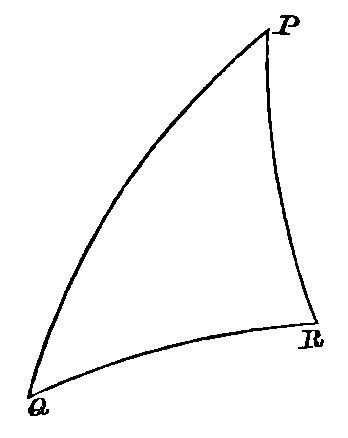
\includegraphics[width=0.3\textwidth]{406.png}
\centering
\end{figure}

Let \(R\) be any point on the surface; let \(PQ = \beta\), \(QR = u\),
\(PR = z\); and let \(PQR = \pi-\psi\), so that \(\psi\) is the angle between
\(RQ\) and \(PQ\) produced. Let the polar radius be denoted by 1,
%%-----File: 407.png-----%%
and the radius at \(R\) by \(1 + \alpha F(z)\), where \(\alpha\) is a small quantity.
Then proceeding as in Art.\ 424, we find that the element of the
required attraction, estimated \textit{from} the pole, to the order we have
to regard
\begin{align*}
&= \frac{du\,d\psi \sin u \cos \psi \cos \frac{1}{2} u} {4\sin^{2} \frac{1}{2} u} \alpha F(z)\\
&= \frac{du\,d\psi \sin^2 u \cos \psi} {8 \sin^{3} \frac{1}{2} u} \alpha F(z)\\
&= \frac{du\,d\psi \sin^2 u \cos \psi} {2^{\frac{3}{2}} (1 - \cos u)^{\frac{3}{2}}} \alpha F(z)\text{.}
\end{align*}

This agrees with D'Alembert's formula at the top of his
page 26; his \(\Delta\) is our \(\psi\).

The transverse attraction which we require would be obtained
by integrating the above expression between the limits \(0\) and
\(2\pi\) for \(\psi\), and \(0\) and \(\pi\) for \(u\). Let \(T\) denote this transverse attraction.

Let \(V\) denote the attraction at \(Q\) resolved along the radius;
and \(\chi\) the angle between this radius and the tangent to \(QP\) at \(Q\).
Then \(V \cos \chi\) is the resolved part of \(V\) along the tangent to
\(QP\) at \(Q\). Hence, supposing the body to be fluid, or at least
the outer stratum to be fluid, we must have for equilibrium
\[
V \cos \chi = T \tag{1}.
\]

If the body rotates, then to secure relative equilibrium, we
must supply in this equation a term corresponding to the resolved
centrifugal force.

We must now give some specific form to \(F(z)\) before we can
carry the investigation further. Assume, with D'Alembert, that
\[
F(z) = A + B \cos z + C \cos^2 z + \ldots + M \cos^m z\text{.}
\]

We shall then have to our order of approximation
\[
\cos \chi = - \sin \beta (B + 2C \cos \beta + \ldots + mM \cos^{m-1}\beta) \alpha;
\]
and it will be sufficient in (1) to put \(\xp\dfrac{4\pi}{3}\) for \(V\). Thus (1) becomes
\[
- \frac{4\pi\alpha}{3} \sin \beta (B + 2C \cos \beta + \ldots + mM \cos^{m-1} \beta) = T \tag{2}\label{576:1}\text{.}
\]
%%-----File: 408.png-----%%

Now \(\cos z = \cos \beta \cos u - \sin \beta \sin u \cos \psi\). Hence, corresponding
to the term \(M \cos^m z\) in \(F(z)\) we have in \(T\) the term
\[
\frac{\alpha M}{2^{\frac{3}{2}}} \int_{0}^{\pi} \int_{0}^{2\pi} \frac{\sin^2 u \cos \psi (\cos \beta \cos u - \sin \beta \sin u \cos \psi)^m}{(1 - \cos u)^{\frac{3}{2}}} du\,d\psi\text{.}
\]

When we integrate with respect to \(\psi\) all the terms which involve
odd powers of \(\cos \psi\) vanish; so that we are left with
\[
- \frac{\alpha M}{2^{\frac{3}{2}}} \int_{0}^{\pi} \int_{0}^{2\pi} \frac{\sin^2 u\, Z\, du\,d\psi}{(1 - \cos u)^{\frac{3}{2}}}
\]
where
\begin{align*}
Z &= m \cos^{m-1} \beta \sin \beta \cos^{m-1} u \sin u \cos^2 \psi\\
&+ \frac{m(m-1)(m-2)}{\oldfactorial{3}} \cos^{m-3} \beta \sin^3 \beta \cos^{m-3} u \sin^3 u \cos^4 \psi\\
&+\ldots
\end{align*}

Here every term involves some odd power of \(\sin \beta\). Now
suppose we put \((1 - \cos^2 \beta) \sin \beta\) for \(\sin^3 \beta\), and \((1 - \cos^2 \beta)^2 \sin \beta\)
for \(\sin^5 \beta\), and so on. Then \(Z\) takes the form
\[
\sin \beta (N_1 \cos^{m-1} \beta + N_3 \cos^{m-3} \beta + N_5 \cos^{m-5} \beta + \ldots)\text{,}
\]
where \(N_1\), \(N_3\), \(N_5\), \dots\ are functions of \(u\) and \(\psi\).

In like manner the other terms in \(F(z)\) will give rise to corresponding
terms in \(T\), involving the product of \(\sin \beta\) into various
powers of \(\cos \beta\); but these powers of \(\cos \beta\) will all be less than
the \((m-1)^{\text{th}}\) power.

Hence equating the coefficients of like terms in (2), we see
that besides other relations we must have
\[- \frac{4\pi m}{3} = - \frac{1}{2^{\frac{3}{2}}} \int_{0}^{\pi} \int_{0}^{2\pi} \frac{N_1 \sin^2 u\,du\,d\psi}{(1-\cos u)^{\frac{3}{2}}}\tag{3}.\]

D'Alembert then has to shew that equation (3) cannot be
satisfied if \(m\) be a positive integer greater than 2. His demonstration,
however, fails completely, because he has given a wrong
value to the quantity which we denote by \(N_1\): his error begins
with his Article 50, on his page 26.
%%-----File: 409.png-----%%

Take the second term which we have expressed in the value
of \(Z\); and put \(\sin \beta (1 - \cos^2 \beta)\) for \(\sin^3 \beta\): then we have as
part of \(N_1\)
\[
- \frac{m(m-1)(m-2)}{\oldfactorial{3}} \cos^{m-3} u \sin^3 u \cos^4 \psi.
\]

Instead of keeping this, D'Alembert puts \(\sin u (1 - \cos^2 u)\)
for \(\sin^3 u\), and then omits \(\sin u\), retaining only \(-\sin u \cos^2 u\), so that
instead of what we have just given, he has
\[\frac{m(m-1)(m-2)}{\oldfactorial{3}} \cos^{m-1} u \sin u \cos^4 \psi.\]

He treats the other terms of \(Z\) in the same unwarrantable
manner; and the consequence is that his value of \(N_1\) is altogether
wrong. The error renders all the rest of his argument
worthless.

Laplace, as we shall see, alludes in his first and second memoirs
to D'Alembert's demonstration, but says nothing about its unsoundness.
Legendre, who may be considered to have been the
first to solve the problem here involved, does not even allude to
D'Alembert's demonstration.

\Section
577. It is important to notice what D'Alembert's process
would have established if it had been sound. It would have
shewn that \(F(z)\) cannot be a \textit{finite} series of powers of \(\cos z\), in
which the highest power is greater than 2. But it would not
have shewn that \(F(z)\) cannot be an \textit{infinite} series of powers of
\(\cos z\).

\Section
578. D'Alembert gives on his page 29 the value of the definite
integral \(\xxp\displaystyle\int_{1}^{-1}{\frac{x^{m-1} dx}{(1-x)^{\frac{1}{2}}}}\) when for \(m\) we put \(1\), \(2\), \(3\), \(4\), \(5\), \(6\), or \(7\).
There is no objection to his method. We may, if we please,
transform the integral to \(\xxp 2(-1)^{m} \displaystyle\int_{0}^{\xsurd2} {(y^2 - 1)^{m-1}} dy\): thus it is easy
to verify his values.

After leaving this subject, D'Alembert on his pages 36\dots 40,
makes a few other remarks; they are not of great importance, but
%%-----File: 410.png-----%%
they are correct, except those contained in his Art.\ 78, which
are erroneous.

\Section
579. The sixth volume of D'Alembert's \textit{Opuscules Mathématiques}
was published in 1773; a large part of it is devoted
to our subject.

\Section
580. A memoir entitled \textit{Sur la Figure de la Terre}, occupies
pages 47\dots 67. It begins thus:

\begin{squote}
Feu M. Maclaurin est le premier qui ait démontré rigoureusement
qu'une masse fluide homogene, tournant autour d'elle-même, devoit
prendre la figure d'une ellipse dans l'hypothèse de l'attraction en raison
inverse du quarré des distances. Mais personne, que je sache, n'avoit
encore remarqué que dans ce cas le problême est susceptible de deux
solutions, c'est-à-dire, qu'il y a deux figures possibles à donner au spheroïde,
et dans lesquelles l'équilibre aura lieu. Cette considération est
l'objet des Recherches suivantes.
\end{squote}

We have already remarked that Thomas Simpson had implicitly
shewn the possibility of this double solution: see Art.\ 285.
However, D'Alembert now gives an explicit investigation, which,
in substance, was afterwards incorporated by Laplace in the
\textit{Mécanique Céleste}, and thus constitutes a permanent part of the
subject: see the \textit{Mécanique Céleste}, Livre \textsc{iii.}, Chapitre \textsc{iii.}

On his page 47, D'Alembert makes the undemonstrated assertion,
that if a spherical mass of homogeneous fluid be put in
rotation it \textit{will} take the form of an oblatum: see Art.\ 575.

\Section
581. We will, in giving an account of D'Alembert's process,
adopt to a great extent Laplace's notation.

Suppose \(\omega\) the angular velocity of rotation, \(\rho\) the density of the
fluid; put \(q\) for \(\genfrac{}{}{1.5pt}{0}{\omega^2}{\dfrac{4\pi\rho}{3}}\). Suppose the major axis of the Earth to be
\(\xsurd (\lambda^2 + 1)\) times the minor axis; then the excentricity of the
ellipse is \(\xxp\dfrac{\lambda}{\xsurd(\lambda^2 + 1)}\). Denote the minor axis by \(2c\). Then by the
%%-----File: 411.png-----%%
formulæ of Art.\ 261, or by those of any elementary work on
Statics we find that the attraction on a particle at the pole is
\[
\frac{4\pi \rho c (1 + \lambda^2)} {\lambda^2} \left\{1- \frac{\tan^{-1} \lambda}{\lambda} \right\};
\]
and the attraction on a particle at the equator is
\[
\frac{2\pi \rho c \xsurd (\lambda^2 + 1)}{\lambda^2} \left\{(1 + \lambda^2) \frac{\tan^{-1}\lambda}{\lambda} - 1 \right\}\text{:}
\]
call the latter \(X\), and the former \(Y\).

The centrifugal force at the equator
\[
= c \xsurd (\lambda^2 + 1) \omega^2 = \frac{4\pi \rho cq}{3} \xsurd(\lambda^2 + 1).
\]

Then, as in Art.\ 262, the condition for relative equilibrium is
\[
\frac{X - \dfrac{4\pi \rho cq}{3} \xsurd(\lambda^2 + 1)}{Y} = \frac{1}{\xsurd(\lambda^2 + 1)},
\]
which reduces to
\[
\frac{2q}{3} = \frac{(\lambda^2 + 3) \tan^{-1} \lambda - 3\lambda}{\lambda^3} \tag{1}.
\]

This is the standard equation on the subject: see the \textit{Mécanique
Céleste}, Livre \textsc{iii.}\ § 18. D'Alembert has the same equation:
see his page 50. He uses \(k\) for Laplace's \(\lambda\), and \(\omega\) for Laplace's \(q\).
Neither D'Alembert nor Laplace uses the symbol \(\tan^{-1}\), which is of
more recent origin. It will be observed that if a sphere of the
same density as the fluid were to rotate with the same angular
velocity, \(q\) would be the ratio of the centrifugal force to the
attraction at the equator.

D'Alembert shews that the equation (1) will give two values
of \(\lambda\) for a given value of \(q\), provided \(q\) be not too great. Denote
by \(\phi (\lambda)\) the right-hand member of equation (1); then considering
\(\lambda\) as an abscissa, and \(\phi (\lambda)\) as the corresponding ordinate, he
in fact traces the curve which thus arises. We have \(\phi (\lambda)\) zero
when \(\lambda\) is zero, and also when \(\lambda\) is infinite; when \(\lambda\) is very small
\(\phi (\lambda)\) is approximately equal to \(\xp\dfrac{4\lambda^2}{15}\). Since \(\phi (\lambda)\) vanishes when
%%-----File: 412.png-----%%
\(\lambda\) vanishes, and when \(\lambda\) is infinite, there must be some maximum
value of \(\lambda\); this maximum is determined by putting \(\phi'(\lambda) = 0\);
this leads to
\[
\tan^{-1}\lambda = \frac{9\lambda + 7\lambda^3}{(1 + \lambda^2)(9 + \lambda^2)} \tag{2}.
\]

It is evident from what has been said that this equation must
have a root. We may also establish the existence of a root in the
following way. When \(\lambda\) is very small the left-hand member is
approximately
\[
\lambda - \frac{\lambda^3}{3} + \frac{\lambda^5}{5} - \ldots,
\]
and the right-hand member is approximately
\[
\lambda - \frac{\lambda^3}{3} + \frac{7\lambda^5}{27} - \ldots;
\]
thus, when \(\lambda\) is very small, the right-hand member is the larger.
When \(\lambda\) is infinite the left-hand member is the larger. Hence
for some intermediate value the two members will be equal. See
D'Alembert's pages 51 and 52.

\Section
582. Suppose that \(q\) has a given value; let \(\lambda_{1}\) denote the
smaller of the two values which equation (1) furnishes. By comparing
the weights of a polar and an equatorial column of fluid,
without assuming that there is equilibrium, D'Alembert finds that
if \(\lambda\) is a little less than \(\lambda_{1}\) the weight of the polar column predominates,
and that if \(\lambda\) is a little greater than \(\lambda_{1}\) the weight of the
equatorial column preponderates. Then he argues thus: Let the
fluid be in relative equilibrium with the value \(\lambda_{1}\). Suppose the
oblatum a little elongated; this amounts to diminishing \(\lambda\); then
the weight of the polar column preponderates, and pushes out the
equatorial column: thus there is a tendency to restore the equilibrium
figure. Again, suppose that we start from the equilibrium
figure, and compress it a little; this amounts to increasing \(\lambda\); then
the weight of the equatorial column preponderates, and pushes
out the polar column: thus there is a tendency to restore the
equilibrium figure. Hence in modern language the relative equilibrium
is \textit{stable}; D'Alembert uses the word \textit{ferme}.
%%-----File: 413.png-----%%

In like manner he concludes that the relative equilibrium corresponding
to the larger of the two values which equation (1)
furnishes is unstable.

His discussion on these points will be found on his pages 55\dots 57:
it cannot be considered adequate for such a difficult matter. I do
not find that the later writers Laplace, Poisson, and Pontécoulant
have followed D'Alembert in determining the stability or instability.

If the angular velocity is such as corresponds to a single solution,
so that (1) and (2) are simultaneously satisfied, D'Alembert
arrives at what he considers a singular result. This result expressed
in modern language is that the relative equilibrium is
stable with respect to an elongation of the oblatum, and unstable
with respect to a compression of the oblatum: see his page 57.

\Section
583. On his page 58, D'Alembert says:

\begin{squote}
Ceci me porteroit à croire, pour le dire en passant, que dans les
Théories données jusqu'ici sur la Figure de la Terre, on a peut-être trop
cherché à faire accorder entr'eux les deux principes, celui de la perpendicularité
de la pesanteur à la surface, et celui de l'équilibre des colomnes.
Car ce dernier n'est nécessaire que quand la Terre est fluide, et n'est
jamais suffisant, soit que la Terre soit solide ou fluide; au lieu que le
premier est nécessaire dans les deux cas, et suffit si la Terre est solide.
\end{squote}

By the principle of columns he probably means the balancing
of columns \textit{at the centre}. Boscovich had shewn that if at \textit{every}
point \textit{every} pair of rectilinear columns balances, then also Huygens's
principle of equilibrium is satisfied: see Boscovich's \textit{De Litteraria
Expeditione \dots} page 424; and Art.\ 463.

\Section
584. When the angular velocity is very small, one of the
forms of relative equilibrium determined by equation (1) is
very nearly spherical, and the other is very much compressed;
D'Alembert calls this a \textit{singulier paradoxe}: see his page 58.

Let us suppose that \(q\) is very small; one value of \(\lambda\) is very
large as we have said. Thus (1) becomes approximately
\[
2q = \frac{3\lambda^2\dfrac{\pi}{2} }{\lambda^3} = \frac{3\pi}{2\lambda};
\]
%%-----File: 414.png-----%%
therefore
\[\lambda = \frac{3\pi}{4q}\tag{3}.\]

Let \(r\) be the radius of a sphere having the same volume as
the oblatum; then with the notation of Art.\ 581,
\[(\lambda^2+1)c^3 = r^3\tag{4}.\]

D'Alembert shews that the velocity of a point at the equator
is very small when \(\lambda\) is very great; that is, the smallness of the
angular velocity more than counterbalances the largeness of the
radius.

For the square of this velocity
\begin{gather*}
= (\lambda^2+1)c^2\omega^2 = (\lambda^2+1)c^{2}\frac{ 4\pi\rho}{3} q\\
\begin{aligned}
&= r^2(\lambda^2+1)^{\frac{1}{3}}\frac{4\pi\rho}{3} q\text{ by (4) } &&= r^2\lambda^{\frac{2}{3}}\frac{4\pi\rho}{3}q \text{ approximately}\\
&= r^2 \left(\frac{3\pi}{4q}\right)^{\frac{2}{3}}\frac{4\pi\rho}{3} q\text{ by (3) } &&= \frac{2r^2\pi^{\frac{5}{3}}q^{\frac{1}{3}}\rho}{\sqrt[3]{6}}\text{:}
\end{aligned}
\end{gather*}
this is small since \(q\) is small.

D'Alembert also compares the centrifugal force at the equator
in this case with the centrifugal force at the equator of the sphere
of equal volume. The ratio of the former to the latter
\[=\frac{\xsurd(\lambda^2+1)c\omega^2}{r\omega^2} = (\lambda^2+1)^{\frac{1}{6}}\text{:}\]
this is large since \(\lambda\) is large. See his page 59; there are misprints
towards the bottom of the page.

\Section
585. D'Alembert was aware that his investigations did not
shew that there could \textit{not be more} than two forms of relative
equilibrium corresponding to a given angular velocity. He expressly
leaves this point to be discussed by other Geometers: see
his page 61. Laplace was the first who demonstrated that there
could not be more than two forms of relative equilibrium: see
D'Alembert's \textit{Opuscules Mathématiques}, Vol.\ \textsc{viii}.\ page 292, and
Laplace's \textit{Théorie \dots\ de la Figure des Planetes}, page 124.

\Section
586. The proposition which D'Alembert thus left to be demonstrated
amounts to this, that \(\phi'(\lambda)\) vanishes \textit{only once} as \(\lambda\)
%%-----File: 415.png-----%%
changes from zero to infinity, besides when \(\lambda = 0\); D'Alembert
draws his curve consistently with this proposition, though he did
not demonstrate it. The proposition is known to be true as it is
indirectly involved in Laplace's investigations; but it may be
useful to give a direct demonstration.

Put \(\tan \theta\) for \(\lambda\); then \(\phi(\lambda)\)
\begin{gather*}
= \frac{(3 + \tan^2\theta) \theta - 3 \tan\theta}{\tan^3\theta} = \frac{(1 + 2\cos^2\theta) \theta - 3 \sin\theta\cos\theta} {\sin^3\theta} \cos\theta\\
= \frac{\theta (1 + 2\cos^2\theta)\cos\theta}{\sin^3\theta} - 3\cot^2\theta\text{.}
\end{gather*}

The differential coefficient of this with respect to \(\theta\) is
\[
\frac{\cos\theta (8+\cos 2\theta)}{\sin^3\theta} - \frac{(5+4\cos 2\theta) \theta}{\sin^4\theta} = \frac{\sin 2\theta (8+\cos 2\theta) - 2\theta (5+4\cos 2\theta)}{2\sin^4\theta}\text{.}
\]
Put \(F(\theta)\) for the numerator.

When \(\theta\) is very small, we shall find that \(F(\theta) = \xp\dfrac{16\theta^5}{15}\). This is
easily obtained by expansion, for
\[
F(\theta) = 8 \sin 2\theta + \frac{1}{2} \sin 4\theta - 2\theta(5 + 4 \cos 2\theta)\text{.}
\]
Or we may proceed thus: we know that when \(\lambda\) is very small
\({\phi(\lambda) = \xp\dfrac{4\lambda^2}{15}}\), so that \(\phi'(\lambda)\) then \(= \xp\dfrac{8\lambda}{15}\); hence when \(\theta\) is very small
we must have \(\xp\dfrac{F(\theta)}{2(\sin\theta)^4} = \xp\dfrac{8\theta}{15}\), and therefore \(F(\theta) = \xp\dfrac{16\theta^5}{15}\).

When \(\theta = \xp\dfrac{\pi}{2}\) we see that \(F(\theta)\) is negative.

If then \(F(\theta)\) vanishes for more than one value of \(\theta\), besides
\(\theta = 0\), between \(\theta = 0\) and \(\theta = \xp\dfrac{\pi}{2}\), it must vanish for three values:
and then \(F'(\theta)\) must vanish for two values of \(\theta\) besides \(\theta = 0\). But
\begin{align*}
F'(\theta) &= 8 \cos 2\theta + 2\cos 4\theta - 10 + 16\theta \sin 2\theta;\\
F''(\theta)& = - 8 \sin 4\theta + 32\theta \cos 2\theta = 16 \cos 2\theta (2\theta - \sin 2\theta).
\end{align*}
%%-----File: 416.png-----%%

Thus \(F''(\theta)\) is positive from \(\theta = 0\) to \(\theta = \xp\dfrac{\pi}{4}\), and then negative
from \(\theta = \xp\dfrac{\pi}{4}\) to \(\theta = \xp\dfrac{\pi}{2}\); therefore \(F' (\theta)\) increases continually from
\(\theta = 0\) to \(\theta = \xp\dfrac{\pi}{4}\), and diminishes continually from \(\theta = \xp\dfrac{\pi}{4}\) to \(\theta = \xp\dfrac{\pi}{2}\):
hence \(F' (\theta)\) cannot vanish more than once besides \(\theta = 0\), as \(\theta\)
changes from \(0\) to \(\xp\dfrac{\pi}{2}\).

\Section
587. We may put equation (1) in the form
\[
\frac{2\lambda^3q}{3} = (\lambda^2 + 3) \tan^{- 1}\lambda - 3\lambda\text{.}
\]

If we suppose \(\lambda = 0\), both sides vanish whatever may be the
value of \(q\). But \(\lambda = 0\) is not a solution of (1); we have in fact
introduced this solution by multiplying both sides of (1) by \(\lambda^3\).

D'Alembert devotes his page 62 to this matter; which would
now be considered too obvious to need remark.

\Section
588. D'Alembert gives some extension to his investigation
on his pages 63\dots 67 by supposing extraneous forces to act; but
this extension is of little importance. D'Alembert afterwards
returns to the subject and discusses it in an elaborate manner:
see Art.\ 596.

At the top of his page 64, D'Alembert seems to say he has
four forces; but his first force is in fact resolved into his second
and third, and is not in addition to them.

\Section
589. The next memoir in the sixth volume of D'Alembert's
\textit{Opuscules Mathématiques} is entitled \textit{Eclaircissemens sur deux
endroits de mes Ouvrages, qui ont rapport à la Figure de la Terre};
this occupies pages 68\dots 76: it is followed by some \textit{Remarques
sur l'Article précédent} on pages 77\dots 84.

The passages in his previous works to which D'Alembert here
alludes occur on page 42 of the \textit{Réflexions \dots\ des Vents}, and on
pages 246\dots 252 of the first volume of the \textit{Opuscules Mathématiques}:
see Arts.\ 376, 378, 514, and 567.
%%-----File: 417.png-----%%

\Section
590. We have already learned from Art.\ 567, that Boscovich
criticised D'Alembert, and that D'Alembert defended himself.
Boscovich's work was translated into French, and a long note
inserted on pages 449\dots 453 which renewed the attack on
D'Alembert: and now D'Alembert replies.

The matters in controversy admit of being stated briefly
though neither of the disputants defines them very clearly.

The translator ascribes great merit to Boscovich for introducing
the notion of what we should call the \textit{stability} of the
equilibrium: D'Alembert replies that the notion is really due
to Daniel Bernoulli. Next as to mathematical results we may
say that both disputants accepted the formula of Art.\ 376; and
also both allowed that the equilibrium would be stable if \(\rho\) were
less than \(\xp\dfrac{5}{3} \sigma\). Then D'Alembert asserts that we may have \(\rho\) less
than \(\xp\dfrac{5}{3} \sigma\), and \(\epsilon'\) positive, and yet have \(\epsilon\) negative; and the formula
of Art.\ 376 shews that his statement is correct. The French
translator denies this, and so is wrong; he seems to have assumed
that \(1 - \xp\dfrac{\rho}{\sigma}\) must be positive, which is not necessary.

The following passage of the translator's note relates to the
opinion which D'Alembert held of Boscovich.

\begin{squote}
\dots\ M. d'\textit{Alembert} se contente ici de dire \textit{qu'il a du nom dans les
mathématiques}: dans un autre opuscule postérieur, il parle du P. \textit{Boscovich}
avec éloge, en disant qu'il mérite la réputation dont il jouit; mais pour
ajouter qu'il a été tellement persécuté par les Supérieurs de son Ordre,
que toute l'autorité du Souverain Pontife a à peine suffi pour le délivrer
de leurs poursuites. Cependant on sait très bien que le R. P. \textit{Boscovich}
a toujours été considéré et respecté dans sa Compagnie comme un de ses
plus dignes membres, et comme un homme du premier mérite à tous
égards.
\end{squote}

On page 71 of the memoir by D'Alembert which we are now
considering he uses the words \textit{habile Mathématicien}, I presume
with reference to Boscovich. It has been asserted in recent times
that D'Alembert and Lagrange had but a low opinion of Boscovich;
see Arago's \textit{Œuvres complètes}, Vol.\ \textsc{ii}.\ page 140.
%%-----File: 418.png-----%%

\Section
591. D'Alembert states on his page 75 his objection to the
formula which Clairaut gave on his page 226. I have discussed
the point in Art.\ 328. D'Alembert admits on his page 82 that
Clairaut's more general formula on page 217 would supply all that
was needed.

D'Alembert quotes in his own favour, with respect to his
controversy with Boscovich's translator, a passage from a letter to
himself, written as he says, by one of the greatest geometers of
Europe: see his page 83.

\Section
592. The next memoir in the sixth volume of D'Alembert's
\textit{Opuscules Mathématiques} is entitled \textit{Sur l'effet de la pesanteur au
sommet et au pied des Montagnes} and more briefly \textit{Sur l'attraction
des Montagnes}; this occupies pages 85\dots 92: it is followed by an
\textit{Addition à l'Article précédent} on pages 93\dots 98.

\Section
593. A certain observer had reported that on the summit of a
mountain in the Alps, \(1085\) toises high, a seconds pendulum had
gained \(28\) minutes in two months; so that gravity appeared
to be greater at the summit of the mountain than at its base.
D'Alembert proposes to shew how the fact may be explained,
assuming the observation to be accurate.

D'Alembert investigates the attractions of mountains of various
shapes. The investigations are simple and satisfactory. In one
case he supposes the mountain to be cylindrical, its height being
small compared with the radius; he obtains a result which was
first given by Bouguer, and has since passed into the elementary
books: see Art.\ 363.

D'Alembert also investigates the influence exerted on a pendulum
when it is placed in a valley between two mountains.

If \(\rho\) be the mean density of the Earth, and \(\rho'\) that of the
mountain, D'Alembert finds that supposing we accept the observation
on the Alps as trustworthy we must have \(\rho'=\xp\dfrac{8\rho}{3}\). This we
should now consider to be quite inadmissible, and so we should
have no faith in the observation. But at the date of the memoir
%%-----File: 419.png-----%%
the state of knowledge was different; and D'Alembert says on his
pages 90, 91:

\begin{squote}
\dots\ cette hypothèse n'a rien de forcé; puisqu'on peut très bien supposer
que la densité moyenne de la Terre est moindre que la densité des
couches qui sont à sa surface.
\end{squote}

The words are hardly fair; for the formula would make the
mean density of the Earth scarcely one-third of that of the mountain.

D'Alembert refers on his page 92 to Bouguer's work on the
Figure of the Earth, pages 357 and following. D'Alembert says:

\begin{squote}
On y trouve une Théorie de l'Attraction des Montagnes, mais beaucoup
moins générale que celle qui a été l'objet de ce Mémoire.
\end{squote}

\Section
594. On his page 93 D'Alembert refers to new observations
with which he had become acquainted long after he had finished
the preceding memoir. These observations seemed to shew that
in a certain district of the Alps, attraction in ascending the mountains
varied directly (not inversely) as the square of the distance
from the centre of the Earth. He traces the consequence of this
hypothesis.

Let \(h\) be the height of the mountain, \(\rho'\) its mean density, \(\rho\) the
mean density of the Earth, \(r\) its radius. Then by the investigation
referred to in Arts.\ 363 and 593 it appears that the attraction
at the top of the mountain is \(\xp\dfrac{4\pi\rho r^3}{3(r + h)^2} + 2\pi\rho'h\), that is approximately
\(\xp\dfrac{4\pi\rho r}{3} + 2\pi h\xp\left(\rho'- \dfrac{4\rho}{3}\right)\). If the attraction varies directly as
the square of the distance from the Earth's centre this must be
equal to \(\xp\dfrac{4\pi\rho r}{3} \xp\left(\dfrac{r + h}{r}\right)^2\), that is approximately to \(\xp\dfrac{4\pi\rho r}{3} \xp\left(1 + \dfrac{2h}{r}\right)\).

Hence we have
\[
\frac{4\pi\rho r}{3} \ldot \frac{2h}{r} = 2\pi h \left(\rho' - \frac{4\rho}{3}\right);
\]
this leads to
\[
\rho' = \frac{8\rho}{3}\text{.}
\]
%%-----File: 420.png-----%%

The coincidence of this result with that in Art.\ 593 is certainly
curious; because it is a theoretical inference from observations
which do not seem to have been influenced by theory. However
there can be, I presume, no doubt that the observations must
have been erroneous. Frisi alludes to the matter; see his \textit{Cosmographia},
Vol.\ \textsc{ii.}\ page 142: he seems to treat the observations as
fictitious. He says:

\begin{squote}
Notitiis enim conquisitis undique accepi alpina illa experimenta \dots\
omnino esse supposita, et circa differentiam attractionum in vertice,
et ad pedes montium Bouguerii tantum experimenta superesse quæ
in investigationibus figuræ terrestris locum aliquem semper habere
debeant.
\end{squote}

See also La Lande's \textit{Bibliographie Astronomique}, page 532.

\Section
595. The next memoir in the sixth volume of D'Alembert's
\textit{Opuscules Mathématiques} is entitled \textit{Suite des Recherches sur la
Figure de la Terre}; this occupies pages 99\dots 133; it is followed
by some \textit{Remarques sur le Mémoire précédent} on pages 134\dots 160.

\Section
596. The problem discussed is one which D'Alembert briefly
noticed on pages 63\dots 67 of the volume: a homogeneous mass of
fluid in the form of an ellipsoid of revolution rotates with uniform
angular velocity round its axis of figure, and is supposed to be in
relative equilibrium under its own attraction and the attraction
of a distant body situated on the prolongation of the axis of figure;
then the condition for this relative equilibrium is found and discussed.
Although the problem cannot be considered to be of any
physical importance yet the analytical processes are both interesting
and instructive.

Let \(M\) denote the mass of the distant body, \(h\) its distance from
the centre of the ellipsoid; the axis of revolution of the ellipsoid
when produced passes through \(M\): take this for the axis of \(x\).

Then the distant body exerts an action \(\xp\dfrac{M}{h^2}\) at the centre of the
ellipsoid; and then in the usual way we find that what we may
call the \textit{disturbing} action of the distant body at a point \((x,y)\) is
equivalent to \(\xp\dfrac{2Mx}{h^3}\) and \(\xp\dfrac{My}{h^3}\) parallel to the axes of \(x\) and \(y\) respectively;
%%-----File: 421.png-----%%
the former in the direction in which \(x\) increases,
the latter contrary to the direction in which \(y\) increases.
D'Alembert says nothing about the force \(\xp\dfrac{M}{h^2}\); we must in fact
imagine it to be counteracted by an equal force applied at every
point.

Let us suppose that the equatorial axis of the ellipsoid is
\(m\) times the polar axis; and let \(k = \xsurd (m^2 - 1)\).

Suppose the density of the ellipsoid to be unity: then taking
it to be an oblatum the attractions at \((x,y)\) parallel to the axes of
\(x\) and \(y\) respectively are by Art.\ 581
\[
\frac{4\pi}{k^3} (k^2 + 1)(k - \tan^{-1} k) x \quad \text{and} \quad \frac{2\pi}{k^3} \left\{(k^2 + 1) \tan^{-1} k - k\right\} y.
\]

We have also the centrifugal force \(\omega^2 y\) parallel to the axis of \(y\),
where \(\omega\) is the angular velocity.

Hence putting \(X\) and \(Y\) for the whole forces at \((x,y)\) parallel
to the axes of \(x\) and \(y\) respectively, and estimating these forces
inwards, we have
\begin{align*}
X &= \frac{4 \pi}{k^3} (k^2 + 1) (k - \tan^{-1} k) x - \frac{2Mx}{h^3} ,\\
Y &= \frac{2 \pi}{k^3} \{(k^2 + 1) \tan^{-1} k - k\} y + \frac{My}{h^3} - \omega^2 y.
\end{align*}

Now we may apply Huygens's principle to obtain the condition
of relative equilibrium. Thus \(X\) and \(Y\) must be positive, supposing
\(x\) and \(y\) to be positive; and \({Xdx + Ydy = 0}\), must coincide
with the differential equation to the ellipse which generates the
ellipsoid, that is with \({xdx + \xp\dfrac{ydy}{k^2 + 1} = 0}\). Hence we obtain
\begin{gather*}
\frac{4 \pi}{k^3} (k^2 + 1) (k - \tan^{-1} k) - \frac{2M}{h^3}\\
= (k^2 + 1) \left[ \frac{2\pi}{k^3} \{(k^2 + 1) \tan^{-1} k - k\} + \frac{M}{h^3} - \omega^2\right];
\end{gather*}
and simplifying we have
\[
\frac{\omega^2}{2\pi} - \frac{M}{2\pi h^3} = \frac{(3 + k^2) \tan^{-1} k - 3k}{k^3} + \frac{M}{\pi h^3 (k^2 + 1)}.
\]
%%-----File: 422.png-----%%

This is the fundamental equation of the problem; it agrees
with D'Alembert's on his page 100, though with rather different
notation.

We shall, as in Art.\ 581, put \(\phi(k)\) for
\[\frac{(3 + k^2) \tan^{-1} k - 3k}{k^3}.\]

\Section
597. We have hitherto supposed the ellipsoid of revolution
to be an oblatum. If it be an oblongum our fundamental equation
still holds, only as \(k= \xsurd(m^2 - 1)\), and \(m\) is now less than
unity, \(\phi(k)\) contains impossible quantities which must be transformed.
We have
\[\phi(k) =\frac{ 3 + k^2}{k^2}\ldot\frac{\tan ^{-1} k}{k} - \frac{3}{k^2} = \frac{2 + m^2}{m^2 - 1}\ldot\frac{\tan^{-1} \xsurd (m^2 - 1)}{\xsurd (m^2 - 1)} - \frac{3}{m^2 - 1}.\]

If \(m\) is less than 1, we find that \(\xp\dfrac{\tan^{-1}\xsurd (m^2 - 1)}{\xsurd (m^2 - 1)}\) transforms in
the usual way into \(\xp\dfrac{1}{2\xsurd (1 - m^2)} \log\xp\dfrac{ 1 + \xsurd (1 - m^2)}{1- \xsurd (1 - m^2)}\).

\Section
598. Our fundamental equation may be written thus
\[\frac{\omega^2}{2\pi} - \frac{M}{2\pi h^3} = \phi(k) + \frac{M}{\pi h^3 (k^2 + 1)} = \phi \left\{\xsurd (m^2 - 1)\right\} + \frac{M}{\pi h^3m^2}.\]

We have to consider whether a value or values of \(m\) between
zero and infinity can be found to satisfy this equation. Moreover,
if \(m\) is less than unity, we must consider that the proper form
for \(\phi \xsurd (m^2 - 1)\), free from impossible expressions, is
\[-\frac{m^2 + 2}{2 (1 - m^2)^{\frac{3}{2}}} \log \frac{1 + \xsurd (1 - m^2)}{1 - \xsurd (1 - m^2)} + \frac{3}{1 - m^2};\]
we will denote this by \(\psi(m)\).

That we have obtained the right equation for the case in
which \(m\) is less than unity, may be verified by an independent
investigation of the attraction of an \textit{oblongum} on a particle at its
surface. D'Alembert himself indicates this method of confirming
the result obtained by the ordinary use of imaginary symbols: see
his pages 134, 135.
%%-----File: 423.png-----%%

\Section
599. Let us first consider the range of values of \(\phi(k)\), as \(k\)
increases from zero to infinity.

When \(k\) is very small \(\phi(k)\) is approximately equal to \(\xp\dfrac{4k^2}{15}\), as
may be easily shewn by expansion. And \(\phi(k)\) obviously vanishes
when \(k\) is infinite.

D'Alembert wishes to shew that \(\phi(k)\) is always positive; see
his pages 102 and 103. His demonstration is unsound. He shews
that \({\tan^{-1} k - \xp\dfrac{k}{1 + \frac{1}{3} k^2}}\) is positive when \(k\) is infinitesimal; and he
shews that this expression is positive when \(\xp\dfrac{k}{1 + \frac{1}{3} k^2}\) has its greatest
value, namely, when \(k = \xsurd 3\). It is easy then to see that the expression
must be positive when \(k\) is greater than \(\xsurd 3\). But it does
not necessarily follow that as \(k\) changes from \(0\) to \(\xsurd 3\) the expression
is \textit{always} positive.

We may proceed thus. Put \(u = (3 + k^2) \tan^{-1} k - 3k\); then
\(\xp\dfrac{du}{dk} = 2k \left(\tan^{-1} k - \dfrac{k}{1 + k^2} \right) = 2\tan\theta (\theta - \sin\theta\cos\theta)\), if \(\tan^{-1} k = \theta\).
Thus \(\xp\dfrac{du}{dk}\) is positive while \(k\) changes from zero to infinity; and so
\(u\) continually increases with \(k\) and never vanishes.

Since \(\phi(k)\) is always positive and vanishes both when \(k\) is zero
and when \(k\) is infinite, it follows that \(\phi'(k)\) must vanish, once at
least, within this range of values of \(k\). We have moreover shewn
in Art.\ 586 that \(\phi'(k)\) can vanish only once. We may observe
that D'Alembert draws his diagrams consistently with the fact
that \(\phi'(k)\) vanishes only once, though as we have remarked he
did not demonstrate this.

\Section
600. D'Alembert shews that \(\psi (m)\) is always negative if \(m\)
lies between \(0\) and \(1\). We have, in fact, to shew that
\[
- \frac{2 + m^2}{2 (1 - m^2)^{\frac{3}{2}}} \log \frac{1 + \xsurd(1 - m^2)}{1 - \xsurd(1 - m^2)} + \frac{3}{1 - m^2}
\]
is always negative. D'Alembert's method is rather laborious: see
%%-----File: 424.png-----%%
his page 104. The best way is to expand in powers of \(\xsurd(1 - m^2)\).
Put \(t\) for \(\xsurd(1-m^2)\); then we have
\[
\psi(m) = - \frac{3-t^2}{2t^3} \log \frac{1+t}{1-t} + \frac{3}{t^2}.
\]

Expanding the logarithm we find that
\[
\psi(m) = -4\left\{\frac{t^2}{3\ldot 5} + \frac{2t^4}{5\ldot 7} + \ldots + \frac{nt^{2n}}{(2n+1)(2n+3)} + \ldots \right\}.
\]

Thus as \(m\) increases from zero to unity, we have \(\psi(m)\) always
negative, and numerically \textit{continually} decreasing from infinity to
zero. This \textit{continual} decrease is not mentioned by D'Alembert,
though he draws his diagram consistently with it.

It will be convenient to give also the expansion of \(\phi(k)\).
We have
\[
\phi(k) = \left(1 + \frac{3}{k^2}\right) \frac{\tan^{-1}k}{k} - \frac{3}{k^2};
\]
expand \(\tan^{-1}k\); thus we get
\[
\phi(k) = \frac{4k^2}{3\ldot5} - \frac{8k^4}{5\ldot 7} + \ldots + (-1)^{n-1} \frac{4nk^{2n}}{(2n+1)(2n+3)} + \ldots
\]

Since \(k^2 = m^2 - 1 = -t^2\), we see by comparing these two expansions
that the value of \(\phi\{\xsurd(m^2-1)\}\) suffers no discontinuity
as \(m\) passes through the value unity. This of course might have
been held probable, but now it is demonstrated.

The series for \(\psi(m)\) and \(\phi(k)\) furnish us with an expansion for
\(\phi\{\xsurd(m^2-1)\}\), which will remain convergent for values of \(m\)
between \(0\) and \(\xsurd 2\), the former extreme value being excluded.

\Section
601. Suppose we put \(M=0\) in the fundamental equation of
Art.\ 596; then we see that the equation cannot be solved by a
value of \(m\) less than unity; for the left-hand member would be
positive, and by Art.\ 600 the right-hand member would be
negative. Hence a mass of rotating fluid cannot be in relative
equilibrium if it is in the form of an \textit{oblongum}, the axis of rotation
coinciding with the axis of figure.

D'Alembert does not draw this inference from his formula.
The theorem was first given by Laplace in his \textit{Théorie \dots\ de la
Figure des Planetes}, page 128.
%%-----File: 425.png-----%%

\Section
602. From Arts.\ 599 and 600 we have the following results
as to the value of \(\phi \{\xsurd(m^2 - 1)\}\). When \(m\) increases from zero to
infinity, \({\phi \{\xsurd(m^2 - 1)\}}\) begins by being negative infinity, increases
algebraically, is zero when \(m = 1\), then becomes positive and increases
to a maximum, and finally reduces to zero. In the diagram
we take \(m\) as the abscissa, and \(\phi \{\xsurd(m^2 - 1)\}\) as the ordinate of the
curve, and we consider ordinates \textit{positive} when they are \textit{above} the
straight line \(OM\): D'Alembert reverses this arrangement.

% put here not float
{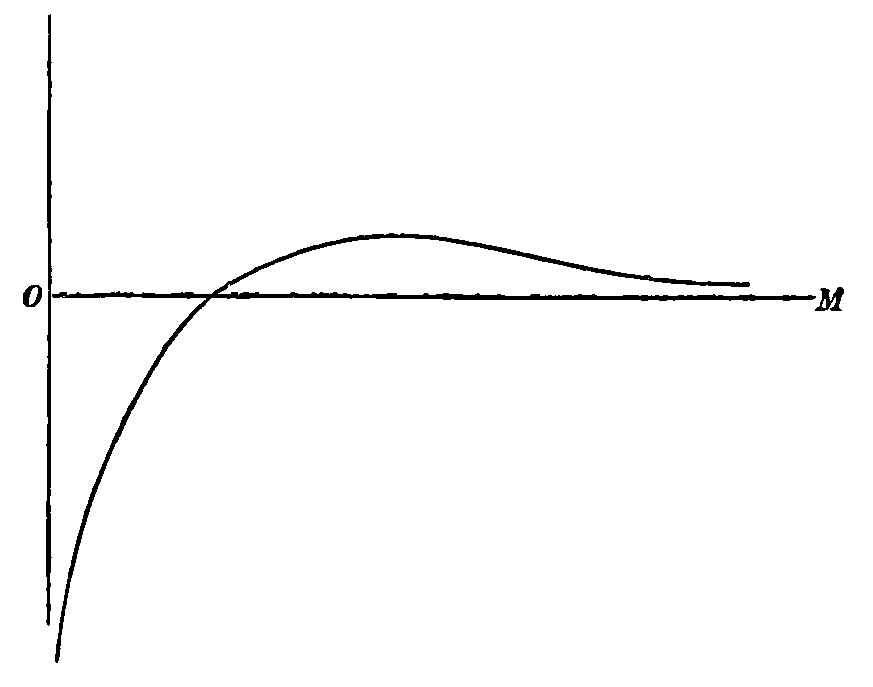
\includegraphics[width=0.7\textwidth]{425.png}
\centering\par}

\Section
603. Next we may proceed to consider the curve, the ordinate
of which is formed by adding to the corresponding ordinate
of the preceding curve the term \(\xp\dfrac{M}{\pi h^3 m^2}\), as required by the fundamental
equation of Art.\ 598.

Put \(f(m)\) for \(\phi \{\xsurd(m^2 - 1)\} + \xp\dfrac{M}{\pi h^3 m^2}\), so that the fundamental
equation becomes
\[\frac{\omega^2}{2 \pi} - \frac{M}{2 \pi h^3} = f(m).\]

When \(m\) is indefinitely small, \(f(m)\) is positive and indefinitely
great; when \(m\) is infinite \(f(m)\) vanishes. Let \(y\) denote an ordinate
corresponding to the abscissa \(m\); then the curve determined
by \(y = f(m)\) may take various forms.

D'Alembert discusses the fundamental equation with great
%%-----File: 426.png-----%%
detail, considering various cases which arise according to the
values of \(\xp\dfrac{\omega^2}{2 \pi} - \xp\dfrac{M}{2 \pi h^3}\) and the different forms of the curve \(y = f(m)\).
We will notice briefly some of the more interesting points which
occur.

Let us consider some of the peculiarities of the curve \(y = f(m)\).

(1) Let \(m_{1}\) denote the value of \(m\) for which \(\phi \{\xsurd(m^2 - 1)\}\) has
its maximum value. If \(\xp\dfrac{M}{\pi h^3}\) is less than \(\phi\{\xsurd({m_1}^2 - 1)\} + \xp\dfrac{M}{\pi h^3 {m_1}^{2}}\),
we have \(f(m)\) greater when \(m = m_{1}\) than when \(m = 1\). And \(f(m)\)
is greater when \(m = m_{1}\) than when \(m = \infty\). Thus \(f(m)\) must have
some maximum value between \(m = 1\) and \(m = \infty\). D'Alembert,
pages 107 and 148.

(2) It is possible that \(f(m)\) should be negative for part of
the range between \(m = 0\) and \(m = 1\). For this merely requires
that \(\xp\dfrac{M}{\pi h^3 m^2} + \psi(m)\) should be negative, or that \(\xp\dfrac{M}{\pi h^3} + m^2 \psi(m)\)
should be negative. Therefore, if \(\xp\dfrac{M}{\pi h^3}\) is less than the numerically
greatest value of \(m^2 \psi(m)\), which is always negative between \(m = 0\)
and \(m = 1\), there will be negative values of \(f(m)\). As \(m^2 \psi(m)\)
vanishes when \(m = 0\) and when \(m = 1\), there will be a numerically
greatest value of \(m\) within this range. D'Alembert, pages 111
and 148.

(3) If, however, \(\xp\dfrac{M}{\pi h^3}\) is greater than the numerically greatest
value of \(m^2 \psi(m)\) within the range from \(m = 0\) to \(m = 1\), then \(f(m)\)
is always positive from \(m = 0\) to \(m = \infty\).

(4) It is possible to have such a value for \(\xp\dfrac{M}{\pi h^3}\) that \(f(m)\) shall
decrease continually from \(m = 0\) to \(m = \infty\); that is, \(f'(m)\) shall
be always negative. D'Alembert, pages 117 and 120.

First, from \(m = 0\) to \(m = 1\). Here we have
\begin{align*}
f'(m) &= \psi'(m) - \frac{2M}{\pi h^3 m^3}\\
&= - \frac{(8 + m^2)m}{2(1 - m^2)^{\frac{5}{2}}} \log \frac{1+\xsurd(1 - m^2)}{1-\xsurd(1 - m^2)} + \frac{7m^2+2}{m(1 - m^2)^2} - \frac{2M}{\pi h^3m^3}.
\end{align*}
%%-----File: 427.png-----%%

This will be negative within the range, if algebraically
\[
\frac{2M }{ \pi h^3} \text{ is greater than } \frac{(7m^2 + 2) m^2 }{ (1-m^2)^2}
- \frac{(8+m^2) m^4 }{2(1 - m^2)^{\frac{5}{2}}}
\log \frac{1 + \xsurd (1 - m^2) }{ 1 - (\xsurd 1 - m^2)}.
\]

The expression on the right-hand side vanishes when \(m = 0\);
and by evaluation it will be found to be \(\xp\dfrac{8}{15}\) when \(m = 1\). It is
always finite between these limiting values; and if \(\xp\dfrac{2M }{\pi h^3}\) is greater
than the algebraically greatest of the values, \(f'(m)\) will be negative
from \(m = 0\) to \(m = 1\).

Next from \(m = 1\) to \(m = \infty\). Here we have
\[
f'(m) = \phi'(k) \frac{dk }{ dm} - \frac{2M }{ \pi h^3 m^3}
= \left\{ \frac{7k^2 + 9 }{ k^3 (1 + k^2)} - \frac{9 + k^2 }{ k^4} \tan^{-1} k \right\}
\frac{m }{ k} - \frac{2M }{ \pi h^3 m^3} ,
\]
where \(k^2 = m^2 - 1\). This will be negative between \(k = 0\) and
\(k = \infty\), if algebraically
\[
\frac{2M }{ \pi h^3} \text{ is greater than } \frac{(k^2 + 1)^2 }{k}
\left\{ \frac{7k^2 + 9 }{ k^3 (k^2 + 1)} - \frac{9 + k^2 }{ k^4} \tan^{-1}k \right\}.
\]

The expression on the right-hand side will be found to be \(\xp\dfrac{8}{15}\)
when \(k = 0\), as it should be from above; and it is negative infinity
when \(k = \infty\). Hence there must be a greatest value among the
positive values which it can take. If \(\xp\dfrac{2M }{ \pi h^3}\) is greater than this
value, \(f'(m)\) will be negative from \(m = 1\) to \(m = \infty\).

If then \(\xp\dfrac{2M }{ \pi h^3}\) be greater than the greatest of the two values
which have thus presented themselves, \(f'(m)\) will be negative
from \(m = 0\) to \(m = \infty\).

\Section
604. The numerical result \(\xp\dfrac{8}{15}\) which occurs in the preceding
Article may be easily verified. In fact, it is the value of \(\psi'(m)\)
when \(m = 1\), or of \(\xp\dfrac{d}{dm} \phi(k)\) which is required. Take the latter;
then we have \(\phi'(k) \xp\dfrac{dk}{dm}\), that is, \(\phi'(k) \xp\dfrac{m}{k}\), that is, by Art.\ 600,
%%-----File: 428.png-----%%
\(\xp\dfrac{m}{k} \left( \dfrac{8k}{15} - \dfrac{32k^3}{35} + \ldots \right)\); and when \(m = 1\) so that \(k = 0\), this becomes
\(\xp\dfrac{8}{15}\). The same result will follow by the aid of Art.\ 600 from the
value of \(\psi'(m)\).

\Section
605. D'Alembert shews that the problem may in certain
cases have two or three solutions for given values of \(\omega\), \(M\) and \(h\).
He makes some remarks as to what we should now call the
\textit{stability} of the relative equilibrium, like the remarks on pages 56
and 57 of the volume which we have noticed in Art.\ 582. See his
pages 112\dots 115, 126\dots 128, 153.

\Section
606. In the fundamental equation of Art.\ 598 put \(m = 1\);
then since \(\phi \{\xsurd(m^2 - 1)\} = 0\) when \(m = 1\), we have
\[
\frac{\omega^2}{2\pi} = \frac{3M}{2\pi h^3}\text{.}
\]

Hence this relation must hold in order that a \textit{sphere} may be a
possible form of relative equilibrium.

\Section
607. When we have obtained a solution of the fundamental
equation, it will still be necessary to advert to the condition
stated in Art.\ 596, that \(X\) and \(Y\) must be positive if \(x\) and \(y\) are,
before we can say that relative equilibrium exists. It will be
sufficient to ensure that one of them is positive, because if the
fundamental equation is satisfied, we know that \(X\) and \(Y\) are of
the \textit{same} sign, supposing \(x\) and \(y\) to be. D'Alembert pays proper
attention to this point: see his pages 105, 116, 117, 122, 123.

Let us, for instance, consider the value of \(Y\). Hence we see
that we must have \(\xp\dfrac{(k^2 + 1)\tan^{-1}k - k}{k^3}\) greater than \(\xp\dfrac{\omega^2}{2\pi} - \xp\dfrac{M}{2\pi h^3}\).
Denote the former expression by \(v\); then it will be found that
\[
\frac{dv}{dk} = \frac{3k - (3 + k^2) \tan^{-1}k}{k^4}.
\]

By Art.\ 599 we see that \(\xp\dfrac{dv}{dk}\) is always negative for real values
of \(k\); and so for such values \(v\) is greatest when \(k = 0\): and then
\(v = \xp\dfrac{2}{3}\).
%%-----File: 429.png-----%%

When we put \(\xsurd(m^2 - 1)\) for \(k\), and suppose \(m\) less than \(1\), we get
\begin{gather*}
\frac{dv}{dm} = \frac{dv}{dk}\frac{dk}{dm} = \frac{m}{k^4} \left\{3 - (3 + k^2) \frac{\tan^{-1}k}{k}\right\}\\
=\frac{ m}{(m^2 - 1)^2} \left\{3 - \frac{m^2+2}{2 \xsurd(1-m^2)} \log \frac{1 + \xsurd(1 - m^2)}{1 - \xsurd(1 - m^2)}\right\}.
\end{gather*}

By Art.\ 600 we know that this is always negative if \(m\) lies
between \(0\) and \(1\); and so for such values \(v\) is greatest when \(m=0\).

But \(v = - \xp\dfrac{m^2}{2(1-m^2)^{\frac{3}{2}}} \log \xp\dfrac{1 + \xsurd(1-m^2)}{1 - \xsurd(1-m^2)} + \xp\dfrac{1}{1 - m^2}\), so that when
\(m = 0\) we have \(v = 1\).

Thus as \(m\) varies from zero to infinity, \(v\) continually diminishes
from unity to zero. See D'Alembert's pages 116, 117, 151, 152.

The fact that \(v\) continually diminishes as \(m\) increases may also
be shewn by putting the value of \(\xp\dfrac{dv}{dm}\) thus:
\[\frac{dv}{dm} = \frac{m}{1 - m^2} \phi \{\xsurd(m^2-1)\};\]
this is always negative, for the factor \(\phi \{\xsurd(m^2 - 1)\}\) is negative
when \(m\) is less than \(1\), and the factor \(\xp\dfrac{m}{1 - m^2}\) is negative when m
is greater than \(1\).

It follows from this discussion that there can be no relative
equilibrium if \(\xp\dfrac{\omega^2}{2\pi}-\xp\dfrac{M}{2\pi h^3}\) is algebraically greater than unity. See
D'Alembert's page 117.

\Section
608. Now let us consider the value of \(X\). Hence we see
that we must have \(\xxp\dfrac{(k-\tan^{-1}k)(k^2+1)}{k^3}\) greater than \(\xp\dfrac{M}{2\pi h^3}\). This
leads us to investigate the greatest value of the former expression.
It will be found that this expression \(= 1 - \xxp\dfrac{(k^2 + 1) \tan^{-1}k - k}{k^3} = 1 - v\);
and as \(v\) continually diminishes from unity to zero, this expression
continually increases from zero to unity. It follows that
there can be no relative equilibrium if \(\xp\dfrac{M}{2 \pi h^3}\) is greater than unity.
See D'Alembert's page 124.
%%-----File: 430.png-----%%

\Section
609. D'Alembert suggests another mode of obtaining solutions
of the problem: see his pages 128\dots 132. Let \(m\) be an
abscissa and \(y\) an ordinate as before; and let \(k = \xsurd(m^2-1)\).
Then draw the curves
\[
y = \frac{2(k-\tan^{-1}k)}{k^3} - \frac{M}{\pi h^3(k^2+1)},
\]
and
\[
y = \frac{(k^2+1)\tan^{-1}k}{k^3}
- \frac{1}{k^2} + \frac{M}{2\pi h^3} - \frac{\omega^2}{2\pi}.
\]

At a point of intersection of these curves the corresponding
value of \(m\) will satisfy the fundamental equation; and if the
value of \(y\) at the point of intersection is positive, the resultant
force at the surface tends \textit{inwards}: therefore with the value of
\(m\) thus obtained relative equilibrium will subsist.

It is sufficient by Art.\ 608 to confine ourselves to the case in
which \(\xp\dfrac{M}{2\pi h^3}\) is less than unity.

In drawing the curves the results obtained in Art.\ 607 will be
found useful. Thus, for instance, the equation to the first curve
may be written
\[
y = \frac{1}{m^2}\left(2 - \frac{M}{\pi h^3} - 2v \right);
\]
and we know that \(v\) diminishes continually from unity to zero as
\(m\) increases from zero to infinity. Hence \(y\) begins by being negative
infinity, vanishes and changes sign once and only once, and
is zero when \(m\) is infinite.

When \(m = 1\) we have \(y = 2 - \xp\dfrac{M}{\pi h^3} - \xp\dfrac{4}{3} = \xp\dfrac{2}{3} - \xp\dfrac{M}{\pi h^3}\); this is positive
or negative according as \(\xp\dfrac{M}{2\pi h^3}\) is less or greater than \(\xp\dfrac{1}{3}\).

\Section
610. Instead of the two curves of the preceding Article,
D'Alembert suggests in his pages 158\dots 160, that we may take the
two curves
\[
y = \frac{2(k^2+1)(k-\tan^{-1}k)}{k^3} - \frac{M}{\pi h^3},
\]
and
\[
y = (k^2+1)\left\{\frac{(k^2+1)\tan^{-1}k}{k^3} - \frac{1}{k^2}
+ \frac{M}{2\pi h^3} - \frac{\omega^2}{2\pi}\right\}.
\]
%%-----File: 431.png-----%%

\Section
611. D'Alembert discusses at some length two analytical
matters which present themselves.

On pages 134\dots 142 he treats of difficulties which may occur
in the use of the symbol \(\xsurd (-1)\). For example, suppose we
require the product of \(\xsurd(-a)\) into \(\xsurd(-b)\). On one hand we
may take for it \(\xsurd (-a \times -b)\), that is, \(\xsurd (ab)\). On the other
hand we may take for it \(\xsurd (a) \times \xsurd (-1) \times \xsurd (b) \times \xsurd(-1)\), that is,
\(\xsurd(ab) \times \xsurd (-1) \times \xsurd (-1)\), that is, \(- \xsurd (ab)\).

On pages 142\dots 145 he shews in various ways that \(x \log x\) is
zero when \(x\) is; and so also is \(x^p \log x^q\) where \(p\) and \(q\) are positive
and finite.

\Section
612. The next memoir in the sixth volume of D'Alembert's
\textit{Opuscules Mathématiques} is also entitled \textit{Suite des Recherches sur
la Figure de la Terre}; this is a continuation of the preceding
memoir; it occupies pages 161\dots 197: it is followed by some
\textit{Remarques sur le Mémoire précédent} on pages 198\dots 210.

\Section
613. In the preceding memoir D'Alembert had considered the
relative equilibrium of a mass of rotating fluid in the form of an
ellipsoid of revolution acted on by the disturbing force of a
distant body, situated on the axis of rotation produced. In the
present memoir he generalises the problem by giving any situation
to the distant body, and by taking for the fluid mass the form of
an ellipsoid, not necessarily of revolution.

\Section
614. We shall use notation more symmetrical than D'Alembert's.

Suppose then that the fluid is in the form of an ellipsoid. Take
the axes of \(x\), \(y\), \(z\) to coincide with the axes of the ellipsoid; let
\(2a\), \(2b\), \(2c\) be the corresponding lengths of the axes. Let there be
a distant body of mass \(M\); and let its co-ordinates be \(l\), \(m\), \(n\)
respectively: put \({R^2 = l^2 + m^2 + n^2}\).

Suppose the fluid to rotate with angular velocity \(\omega\) round an
axis, the direction cosines of which are \(\lambda\), \(\mu\), \(\nu\). We have to form
the conditions for relative equilibrium.

Now here we must observe that the distant body must, in fact,
be supposed to share in this rotation of the fluid mass. D'Alembert
never notices this fact, though it is really involved in his process.
In the particular case of the preceding memoir, in which the
%%-----File: 432.png-----%%
distant body is supposed to be \textit{on} the axis of rotation, we may
practically regard the distant body as fixed; but we cannot in the
present memoir. A particular case of the present memoir, as we
shall see, was afterwards discussed by Laplace; in this case the
Moon is taken to be the fluid mass, and the Earth to be the
distant body. See Laplace's \textit{Théorie \dots\ de la Figure des Planetes},
pages 113\dots 116.

\Section
615. Let \(P\) be any point of the fluid; let \(x\), \(y\), \(z\) be the coordinates
of \(P\). The attraction of the fluid ellipsoid parallel to the
axes of \(x\), \(y\), \(z\) respectively will be \(Ax\), \(By\), \(Cz\) respectively where
\(A\), \(B\), \(C\) are certain constants. D'Alembert in effect briefly states
that this can be easily shewn in the way in which Maclaurin treated
the attraction of an ellipsoid of revolution; this is true, and it is
to be noted that we have here, for the first time, the important
extension of Maclaurin's result from an ellipsoid of revolution to
the general ellipsoid. See D'Alembert's page 165. But as we
shall hereafter point out, Frisi had previously gone some way in
this direction: see his \textit{De Gravitate}, pages 157 and 159.

\Section
616. The attraction of the distant body at \(P\) parallel to the
axis of \(x\) is
\[
\frac{M(l-x)}{\left\{(l-x)^2 + (m-y)^2 + (n-z)^2\right\}^{\frac{3}{2}}};
\]
the \textit{disturbing} part of
this is approximately
\[
- \frac{Mx}{R^3} + \frac{3Ml(lx + my + nz)}{R^5},
\]
say \(- \xp\dfrac{Mx}{R^3} + \xp\dfrac{3Mlu}{R^5}\) where \(u\) is put for \(lx + my + nz\).

It is only the disturbing part of the action of \(M\) which
D'Alembert regards; he makes no allusion to the other part,
that is, \(\xp\dfrac{Ml}{R^3}\) in this case. See Art.\ 596.

Let \(O\) denote the centre of the ellipsoid; let \(Q\) denote the
foot of the perpendicular from \(P\) on the axis of rotation; then
the so-called centrifugal force is \(\omega^2 PQ\), and we require the resolved
part of this. We have to \textit{project} \(PQ\) on the axis of \(x\); and
by a known theorem of projections we may take the difference of
the projections of \(OP\) and \(OQ\) for the projection of \(PQ\).
%%-----File: 433.png-----%%

Thus we obtain \(\xp\omega^2 (OP.\dfrac{x}{OP} - OQ \cos \lambda)\); and this
\begin{align*}
=& \omega^2 (x - OQ \cos \lambda) = \omega^2 (x - OP \cos POQ \cos \lambda)\\
=& \omega^2 \{x - (x \cos \lambda + y \cos \mu + z \cos \nu) \cos \lambda\}\\
=& \omega^2 (x - v \cos \lambda)\text{ where }v\text{ is put for }x \cos \lambda + y \cos \mu + z \cos \nu\text{.}
\end{align*}

Let \(X\) denote the whole force parallel to the axis of x, estimated
inwards; then
\[
X = Ax + \frac{Mx}{R^3} - \frac{3Mlu}{R^5} - \omega^2 (x - v \cos \lambda)\text{.}
\]

Similar expressions hold for the attractions parallel to the
other axes, which we will denote by \(Y\) and \(Z\) respectively.

D'Alembert's method is substantially equivalent to this though
his notation is less symmetrical.

\Section
617. The conditions for relative equilibrium are
\[
X \div \frac{x}{a^2} = Y \div \frac{y}{b^2} = Z \div \frac{z}{c^2}\text{.}
\]

Take the equation \(Xa^2y = Yb^2x\); this must be identically
true, and so we may equate the coefficients of \(xy\), \(x^2\), \(y^2\), \(xz\), \(yz\).
By equating the coefficients of \(xy\) we obtain
\begin{multline*}
a^2 \left\{A + \frac{M}{R^3} - \frac{3Ml^2}{R^5} - \omega^2 (1-\cos^2 \lambda)\right\}\\
= b^2 \left\{B + \frac{M}{R^3} - \frac{3Mm^2}{R^5} - \omega^2 (1-\cos^2 \mu)\right\}.
\end{multline*}

By equating the coefficients of \(x^2\), and by equating the coefficients
of \(y^2\), we arrive at the same condition, namely,
\[
- \frac{3Mlm}{R^5} + \omega^2 \cos \lambda \cos \mu = 0.
\]

By equating the coefficients of \(xz\) we have
\[
- \frac{3Mmn}{R^5} + \omega^2 \cos \mu \cos \nu = 0.
\]

By equating the coefficients of \(yz\) we have
\[
- \frac{3Mnl}{R^5} + \omega^2 \cos \nu \cos \lambda = 0.
\]
%%-----File: 434.png-----%%

In like manner we may take the equation \(Xa^2z = Zc^2x\); by so
doing we shall find that we get only one new condition.

The whole results may be written thus:
\begin{gather*}
\frac{3Mmn }{ R^5} = \omega^2 \cos \mu \cos \nu,\;
\frac{3Mnl }{ R^5} = \omega^2 \cos \nu \cos \lambda,\;
\frac{3Mlm }{ R^5} = \omega^2 \cos \lambda \cos \mu.\\
a^2 \left(A + \frac{M }{ R^3} - \frac{3Ml^2 }{ R^5} - \omega^2 \sin^2 \lambda\right) =
b^2 \left(B + \frac{M}{R^3}-\frac{3Mm^2 }{ R^5} - \omega^2 \sin^2 \mu\right)\\
= c^2 \left(C + \frac{M}{R^3} - \frac{3Mn^2 }{ R^5} - \omega^2 \sin^2 \nu\right).
\end{gather*}

\Section
618. As a particular case of the preceding investigation, suppose
that there is no distant disturbing body; then \(M = 0\); thus
\(\cos \mu \cos \nu = 0\), \(\cos \nu \cos \lambda = 0\), \(\cos \lambda \cos \mu = 0\). Hence two of the
three cosines \(\cos \lambda\), \(\cos \mu\), \(\cos \nu\) must vanish; so that the rotation
must be round one of the principal axes of the ellipsoid. Hence
we see that the case taken in Jacobi's theorem is the only case in
which an ellipsoid of fluid rotating round a diameter can remain
in relative equilibrium. A statement which has been recently
made to the contrary by Dahlander and by Schell is inaccurate:
see the \textit{Proceedings of the Royal Society}, Vol.\ \textsc{xxi.}

\Section
619. Return to the conditions obtained in Art.\ 617. Let us
suppose that \(l\), \(m\), and \(n\) are not zero. The first and the second
of these conditions give
\[
\frac{m }{ l} = \frac{\cos \mu }{ \cos \lambda};
\]
the second and the third give
\[
\frac{n }{ m} = \frac{\cos \nu }{ \cos \mu}.
\]

Hence the radius vector to the distant body coincides in direction
with the axis of rotation; thus
\[
\cos \lambda = \frac{l }{ R},\quad \cos \mu = \frac{m }{ R},\quad \cos \nu = \frac{n }{ R},
\]
and then from any of the first three conditions we get
\[
\frac{3M }{ R^3} = \omega^2;
\]
and the other conditions reduce to
\[
a^2 \left(A - \frac{2M }{ R^3}\right) = b^2 \left(B - \frac{2M }{ R^3}\right)
= c^2 \left(C - \frac{2M }{ R^3}\right);
\]
%%-----File: 435.png-----%%
these last will be satisfied if \(a = b = c\), that is if the fluid mass be
spherical.

The particular case in which the radius vector to the distant
body and the axis of rotation coincide in direction presents
itself in D'Alembert's memoir; but he does not pay much attention
to it: see his page 200.

He also notices a particular case in which it is given that two
of the three \(a\), \(b\), \(c\) are nearly equal: see his page 209.

But he does not notice that we may have a sphere exactly if
\({\xp\dfrac{l}{\cos\lambda} = \xp\dfrac{m}{\cos\mu} = \xp\dfrac{n}{\cos\nu}}\) and \(\omega^2 = \xp\dfrac{3M}{R^3}\).

\Section
620. It will be interesting to enquire if the conditions in the
preceding Article can be satisfied in any other way besides having
\(a = b = c\); this enquiry leads us a little beyond the point at which
the theory of the attraction of ellipsoids had arrived at this date.

Let \(V\) denote the mass of the ellipsoid; then we know that
\[A =\frac{3V}{a} \int_0^1\frac{x^2dx}{\xsurd\{a^2+(b^2-a^2)x^2\}\{a^2+(c^2-a^2)x^2\}};\]

This result was given by Laplace in his \textit{Théorie \dots\ de la Figure
des Planetes}, page 92; as we shall see D'Alembert himself first
obtained it but rejected it in the seventh volume of his \textit{Opuscules
Mathématiques}.

Assume \(x = \xp\dfrac{a}{\xsurd(a^2+s)}\); then we find that
\[A=\frac{3V}{2} \int_0^\infty \frac{ds}{(a^2+s)D},\]
where \(D\) stands for \(\xsurd\{(a^2+s)(b^2+s)(c^2+s)\}\).

In like manner we have
\[B=\frac{3V}{2} \int_0^\infty \frac{ds}{(b^2+s)D},\quad C=\frac{3V}{2} \int_0^\infty \frac{ds}{(c^2+s)D}.\]

Put \(\phi^2\) for \(\xp\dfrac{2M}{R^3}\); then the conditions we have to examine may
be written
%%-----File: 436.png-----%%
\begin{align*}
(a^2 - b^2)\phi^2 &= a^2A - b^2B = \frac{3V(a^2 - b^2)}{2} \int_{0}^{\infty} \frac{sds}{(a^2 +s)(b^2 + s)D},\\
(b^2 - c^2)\phi^2 &= b^2B - c^2C = \frac{3V(b^2 - c^2)}{2} \int_{0}^{\infty} \frac{sds}{(b^2 + s)(c^2 + s)D};
\end{align*}
hence we see that these conditions cannot be satisfied if \(a\), \(b\), \(c\) are
all unequal; for they would lead to two different values of \(\phi^2\).

But suppose two of the three, \(a\), \(b\), \(c\) to be equal; say \(a\) and \(b\):
then our conditions reduce to
\[
\phi^2 = \frac{3V}{2} \int_{0}^{\infty} \frac{sds}{(b^2 + s)(c^2 + s)D};
\]
and this is quite admissible if \(b\), \(c\), \(V\) and \(\phi\) be properly adjusted,
whether \(b\) is greater or less than \(c\).

\Section
621. If \(l\), \(m\), \(n\) are all different from zero we have the case
discussed in the preceding two Articles, in which the radius vector
to the distant body and the axis of rotation coincide in direction.
D'Alembert himself pays little attention to this case: indeed in
his page 200 he seems to consider that it cannot occur. Let
us now return to the general conditions of Art.\ 619; and suppose
that \(l\), \(m\), \(n\) are not all different from zero. Suppose for example
that \(n = 0\); then it follows from the first and second conditions
that either \(\cos \nu = 0\), or else \(\cos \lambda = 0\), and \(\cos \mu = 0\): if we suppose
the latter, then \(l\) or \(m\) must also \(= 0\). In the former case, the axis
of rotation is in the principal plane corresponding to \(a\) and \(b\); in
the latter case the axis of rotation coincides with the axis corresponding
to \(c\). In each case the axis of rotation and the radius
vector to the distant body are both in one of the principal planes
of the fluid mass.

\Section
622. In Arts.\ 619 and 620 we see that the supposed ellipsoid
is either a sphere or an ellipsoid of revolution; and in Art.\ 621
we see that the axis of rotation and the radius vector to the distant
body must be in one of the principal planes of the fluid mass.
Combining these two results, we may say that in every case in
which the relative equilibrium is possible the axis of rotation and
the radius vector to the distant body must be in one of the principal
planes of the fluid mass. D'Alembert arrives at this result,
%%-----File: 437.png-----%%
and confirms it by some general reasoning which is not very cogent:
see his pages 198\dots 200.

\Section
623. As a particular case of Art.\ 617 let us suppose we have
given that the axis of rotation and the radius vector to the distant
body are at right angles. This may be considered to hold with
respect to the moon supposed fluid, the distant body being the
Earth. Since here we have not the case of Arts.\ 619 and 620,
it follows that one or two of the three \(l\), \(m\), \(n \) must be zero. Suppose
\(n = 0\); then from the first two conditions of Art.\ 617, we
shall find either \(\cos \nu = 0\), or both \(\cos \lambda = 0\), and \(\cos \mu = 0\).

I\@. Suppose \(\cos \nu = 0\). Then the third condition is
\[
\omega^2 \cos \lambda \cos \mu = \frac{3Mlm }{ R^5}\text{.}
\]
Now by our hypothesis that the two directions are at right angles,
this would give \(\omega^2 = - \xp\dfrac{3M }{ R^3}\), if we suppose that \(lm\) does not vanish;
this is impossible. Therefore \(lm\) vanishes. Hence we must have
either \(l = 0\), and \(\cos \mu = 0\), or \(m = 0\), and \(\cos \lambda = 0\).

II\@. Suppose \(\cos \lambda = 0\), and \(\cos \mu = 0\).

Then the third condition shews that \(lm = 0\). Therefore either
\(l = 0\), or \(m = 0\).

Hence we must have the axis of rotation coinciding with one
of the principal axes of the body, and the radius vector to the
distant body coinciding with another.

The result might have been anticipated perhaps; and we shall
find that Laplace assumes it as evident: see the reference in
Art.\ 614.

\Section
624. We have seen in Art.\ 622 that the axis of rotation and
the radius vector to \(M\) must always be in one of the principal
planes of the ellipsoid. We will suppose that \(n = 0\), and \(\cos \nu = 0\).
Hence the conditions of Art.\ 617, reduce to
\[
\frac{3Mlm }{ R^5} = \omega^2 \cos \lambda \cos \mu,
\]
%%-----File: 438.png-----%%
\begin{gather*}
a^2 \left\{A + \frac{M}{R^3} - \frac{3Ml^2}{R^5} - \omega^2 \sin^2 \lambda\right\}\\
= b^2 \left\{B + \frac{M}{R^3} - \frac{3Mm^2}{R^5} - \omega^2 \sin^2 \mu\right\}
= c^2 \left\{C + \frac{M}{R^3} - \omega^2\right\}.
\end{gather*}
And in virtue of our supposition that \(n \) and \(\cos \nu\) vanish we have
\[
\cos^2 \lambda + \cos^2 \mu = 1, \quad l^2 + m^2 = R^2.
\]

As to whether these equations are consistent nothing is said
by D'Alembert; we have discussed one case of the general problem
in Arts.\ 619 and 620, but the matter is not of sufficient importance
to detain us longer.

\Section
625. D'Alembert begins on his page 174 an investigation of
the attraction of an ellipsoid on any particle at the surface. This
amounts to seeking the values of the \(A\), \(B\), \(C \) of Art.\ 615.

He makes some simple and useful remarks on his pages 174\dots 176;
we will give an example of them. Suppose the semiaxes of an
ellipsoid to be \(r\), \(r (1 + \alpha)\), and \(r (1 + \beta)\), where \(\alpha\) and \(\beta\) are very
small. Let the approximate value of the attraction be required
for a particle situated at the end of the semiaxis \(r\). We may
assume that this attraction will be \(\xp\dfrac{4\pi r}{3} (1 + p\alpha + q\beta)\), where \(p \) and \(q\)
are certain constants to be determined: this assumption depends on
the fact that if \(\alpha\) and \(\beta\) vanish, the body becomes a sphere, and
the attraction then is \(\xp\dfrac{4\pi r}{3}\). Next we may admit that \(p = q\); because
the attraction ought to remain unchanged if we interchange
the second and third semiaxes. Hence the attraction becomes
\(\xp\dfrac{4\pi r}{3} \{1 + p(\alpha + \beta)\}\). Now we can determine \(p\). For if we suppose
\(\alpha = \beta\) the ellipsoid becomes an ellipsoid of revolution, and the
attraction of such a solid on a particle at the pole is known: hence
equating this known attraction, estimated approximately, to
\(\xp\dfrac{4\pi r}{3} (1 + 2p\alpha)\) we determine \(p\). We should thus get \({p = \xp\dfrac{2}{5}}\).

\Section
626. D'Alembert attempted to find the attraction of an ellipsoid
by decomposing it into slices in various ways; but he does
not succeed in effecting the integrations. We know now that the
%%-----File: 439.png-----%%
result can be expressed by means of elliptic integrals, but not by
circular arcs or logarithms. We will briefly state the methods of
decomposition of the ellipsoid which he tries. The attracted
particle is supposed to be at the end of the semiaxis \(c\).

I\@. Suppose a plane to pass through the attracted particle, and
also through the tangent to the ellipsoid at that point which is
parallel to the axis \(2a\). Let this plane turn round the tangent line
and cut the ellipsoid into wedge-shaped slices: see D'Alembert's
page 180. This decomposition is like that used by Thomas Simpson;
which we have noticed in Art.\ 279.

II\@. Instead of using the tangent parallel to the axis \(2a\), we
may use the tangent parallel to the axis \(2b\).

III\@. Suppose a plane to pass through the axis \(2c \) and to turn
round, and thus cut the ellipsoid into wedge-shaped slices: see
D'Alembert's page 183. This decomposition is like that used by
Maclaurin; which we have noticed in Art.\ 255.

IV\@. Or the ellipsoid may be cut into laminæ by a plane which
is always at right angles to the axis \(2c\): see D'Alembert's page 184.

\Section
627. For the case of an ellipsoid in which two of the axes are
very nearly equal D'Alembert obtains approximate values of
the attraction at the end of the principal axes: see his page 192.
A mistake in the results is corrected on page 424.

The approximate results just referred to are applied by
D'Alembert to the question of relative equilibrium which was
proposed at the beginning of the memoir: see his pages 194\dots 197.
He finishes in a patronising tone:

\begin{squote}
Je ne doute point que cette nouvelle Recherche ne donnât lieu
à plusieurs remarques curieuses; mais je les abandonne à d'autres Géometres,
la matiere n'ayant plus aucune difficulté.
\end{squote}

\Section
628. The next memoir in the sixth volume of D'Alembert's
\textit{Opuscules Mathématiques} is also entitled \textit{Suite des Recherches
sur la Figure de la Terre}; this is a continuation of the preceding
memoir; it occupies pages 211\dots 246: it is followed by some
\textit{Remarques sur le Mémoire précédent} on pages 247\dots 259.
%%-----File: 440.png-----%%

\Section
629. D'Alembert now proposes to extend the problem of the
preceding memoir by supposing several distant attracting bodies
instead of the single distant attracting body there considered.

This extension becomes very easy with the aid of modern symmetrical
notation. Let \(M_1\), \(M_2\), \(M_3\) \dots\ denote the masses of the
various distant bodies respectively; let \(l_1\), \(m_1\), \(n_1\) be the coordinates
of the first body, \(R_1\) its distance; and let similar notation hold with
respect to the other bodies.

Then instead of the first equation of Art.\ 617, namely
\[
\frac{3Mmn}{R^5} = \omega^2\cos\mu\cos\nu,
\]
we now have \(\xp\dfrac{3M_1 m_1 n_1}{{R_1}^5} + \xp\dfrac{3M_2 m_2 n_2}{{R_2}^5} + \xp\dfrac{3M_3 m_3 n_3}{{R_3}^5} + \ldots = \omega^2\cos\mu\cos\nu\),
which we may write thus \(3\sum \xp\dfrac{Mmn}{R^5} = \omega^2\cos\mu\cos\nu\).

\hypertarget{629:1}{Similarly the other equations may be expressed.}

D'Alembert himself does not proceed in this way nor adopt this
notation. He uses spherical trigonometry. It may be observed
that he demonstrates the expression for the cosine of an angle of a
spherical triangle in terms of the sines and cosines of the sides;
he starts from formulæ for a right-angled spherical triangle which
he assumes: see his pages 247 and 248.

As we have remarked in Art.\ 614, the distant bodies must be
supposed to rotate with the fluid mass; though D'Alembert does
not notice this fact. And as in Arts.\ 596 and 616, D'Alembert
says nothing about certain forces which are not what I have called
\textit{disturbing} forces.

\Section
630. The only point which appears to be of any interest in
the problem is a remark which D'Alembert makes on his page 253;
the remark amounts to this: if the axis of rotation and the radii
vectores to the distant attracting bodies are all in one plane that
plane must be a principal plane of the ellipsoid. He does not demonstrate
this, but seems to rely on the principle of symmetry as
in the corresponding theorem for a single distant attracting body:
see Art.\ 622. We will examine the theorem. Suppose that the
equation to the plane is \(\alpha x + \beta y + \gamma z = 0\); so that
%%-----File: 441.png-----%%
\begin{align*}
&\alpha \cos\lambda + \beta \cos\mu + \gamma \cos\nu = 0,\\
&\alpha l_1 + \beta m_1 + \gamma n_1 = 0,\\
&\alpha l_2 + \beta m_2 + \gamma n_2 = 0,
\end{align*}
and so on.

Take the three equations
\begin{gather*}
3\sum \frac{Mmn}{R^5} = \omega^2 \cos\mu \cos\nu, \qquad
3\sum \frac{Mnl}{R^5} = \omega^2 \cos\nu \cos\lambda,\\
3\sum \frac{Mlm}{R^5} = \omega^2 \cos\lambda \cos\mu\text{.}
\end{gather*}

Substitute in the first of these for \(n_1\), \(n_2\), \dots, and for \(\cos\nu\);
thus
\[
3\sum \frac{Mm(\alpha l + \beta m)}{R^5}
= \omega^2 \cos\mu (\alpha \cos\lambda + \beta \cos\mu);
\]
therefore by means of the third equation we obtain
\[
3\sum \frac{Mm^2}{R^5} = \omega^2 \cos^2\mu.
\]

Similarly
\[
3\sum \frac{Ml^2}{R^5} = \omega^2 \cos^2\lambda, \quad
3\sum \frac{Mn^2}{R^5} = \omega^2 \cos^2\nu.
\]

Hence the first of the three equations becomes
\[
\sum \frac{Mmn}{R^5} = \sqrt{\sum \frac{Mm^2}{R^5} \ldot \sum \frac{Mn^2}{R^5}}.
\]

Squaring we get
\begin{gather*}
\left\{\frac{M_1 m_1 n_1}{{R_1}^5} + \frac{ M_2 m_2 n_2}{{R_2}^5} + \frac{M_3 m_3 n_3}{{R_3}^5} + \ldots \right\}^2\\
=\left\{\frac{M_1 {m_1}^2}{{R_1}^5} + \frac{M_2 {m_2}^2}{{R_2}^5} + \frac{M_3 {m_3}^2}{{R_3}^5} + \ldots\right\}
\left\{\frac{M_1 {n_1}^2}{{R_1}^5} + \frac{M_2 {n_2}^2}{{R_2}^5} + \frac{M_3 {n_3}^2}{{R_3}^5} + \ldots\right\}\text{.}
\end{gather*}

This by common Algebra leads to \(\xp\dfrac{m_1}{n_1} = \xp\dfrac{m_2}{n_2} = \xp\dfrac{m_3}{n_3} = \ldots\)

In this way we see that all the radii vectores to the distant
bodies must coincide. Thus the case reduces to that of Art.\ 619.

But suppose, as in fact D'Alembert does, that the plane in
which the axis of rotation and the radii vectores to the distant
bodies lie is perpendicular to a principal plane; let its equation be
\[
\alpha x + \beta y = 0.
\]
%%-----File: 442.png-----%%

Then as before we can obtain from our three equations,
\[3\sum\frac{Ml^2}{R^5} = \omega^2 \cos^2\lambda,\qquad 3\sum\frac{Mm^2}{R^5} = \omega^2 \cos^2\mu;\]
but we do \textit{not} now have also \(3\displaystyle\sum \xp\dfrac{Mn^2}{R^5} = \omega^2 \cos^2\nu\).

The equations which correspond to the last two of Art.\ 617
are
\[a^2 \left\{A + \sum \frac{M}{R^3} - \omega^2\right\} = b^2\left\{B + \sum \frac{M}{R^3} - \omega^2\right\} = c^2 \left\{C - 2\sum \frac{M}{R^3}\right\};\]
for \(\omega^2 \sin^2\nu = \omega^2 (\cos^2\lambda + \cos^2\mu) = 3\sum M\xp\dfrac{l^2 + m^2}{R^5} = 3\sum\dfrac{M(R^2 - n^2)}{R^5}\).

If D'Alembert's remark were universally true the equations
connecting \(a\), \(b\), and \(c\) ought to be impossible, or inconsistent with
the others, if \(a\), \(b\), and \(c\) are unequal. But this does not seem to
be the case. By the method of Art.\ 620, we get from them
\[\omega^2 - \sum\frac{ M}{R^3} =\frac{ 3V}{2} \int_0^\infty \frac{sds}{(a^2 + s)(b^2 + s)D},\]
and
\[2c^2\sum\frac{M}{R^3} = \frac{3V}{2} \int_0^\infty \frac{c^2s + c^2(a^2 + b^2) - b^2a^2}{D^3} sds;\]
and these if \(c^2(a^2 + b^2)-b^2 a^2\) is positive present nothing impossible.

As an example we might suppose two distant bodies, and take
\begin{gather*}
l_1 = 0,\quad m_1= 0,\quad n_1 = R,\\
l_2 = R_2 \cos\lambda,\quad m_2 = R_2 \cos\mu,\quad n_2 = R_2 \cos\nu.
\end{gather*}

Then it will be found that our first three equations give
\(\omega^2 = \xp\dfrac{3M_2}{{R_2}^{3}}\); and we have only to ascertain if this is consistent with
the last two equations, the form of which has just been given.
Thus we have to put
\[\frac{2M_2}{{R_2}^{3}} - \frac{M_1}{{R_1}^{3}} = \frac{3V}{2} \int_0^\infty \frac{(c^2 + s)sds}{D^3},\]
and
\[2c^2 \left(\frac{M_2}{{R_2}^{3}} + \frac{M_1}{{R_1}^{3}}\right) = \frac{3V}{2} \int_0^\infty \frac{c^2 s + c^2(a^2 + b^2) - b^2a^2}{D^3} sds.\]
%%-----File: 443.png-----%%
It will be found that these lead to values of \(\xp\dfrac{M_2}{{R_2}^3}\) and \(\xp\dfrac{M_1}{{R_1}^3}\) which
are certainly positive if \((a^2-c^2)(c^2-b^2)\) is positive; for then
also \(c^2(a^2+b^2)-b^2a^2\) is positive. It is manifest that this condition
\textit{may} be satisfied; and thus D'Alembert's remark is not true.

\Section
631. D'Alembert on his page 216, refers to Maclaurin's Essay
on the Tides, as containing a little matter bearing on the problem
discussed in this memoir; but Maclaurin had not effected much.
Maclaurin did not shew that the figure of an ellipsoid would satisfy
the conditions of equilibrium; nor did he show how to determine
the position of the axes of the ellipsoid. D'Alembert says of his
own memoir: Nous avons de plus démontré dans celui-ci que la
figure du sphéroïde est elliptique\dots. However he does not shew
that the figure \textit{is} an ellipsoid, but only that it \textit{may} be an ellipsoid.

\Section
632. D'Alembert says on his page 217, that he will conclude
with some detached reflexions bearing on the Figure of the Earth.

\Section
633. He says that among the solutions hitherto given of the
problem the only one which is exact is that which supposes the
spheroid to be fluid and homogeneous; the other solutions being
approximations. Suppose that \(\alpha\) is a very small quantity; and
we have found that neglecting \(\alpha^2\) the equation of relative equilibrium
is satisfied for a certain figure; we must not say that this
figure \textit{exactly} satisfies the conditions of relative equilibrium. But
D'Alembert suggests that if we give to the figure a certain small
change of the order \(\alpha^2\) the conditions of relative equilibrium may be
rigorously satisfied; and he considers it a plausible supposition that
there may be an \textit{infinity} of figures in which the relative equilibrium
will subsist rigorously: see his page 223. Probably few persons will
agree with D'Alembert in considering this supposition plausible.

\Section
634. D'Alembert returns on his pages 225\dots 230 and 254\dots 259,
to his favourite equation relating to the ellipticity of fluid surrounding
a solid nucleus: see Arts.\ 376, 430, and 590.

We shall briefly notice some points that arise.

On his pages 227\dots 229, D'Alembert criticises as inexact certain
formulæ on page 247 of Clairaut's work, and thus as affording an
insufficient proof of Clairaut's theorem which is founded on them.
%%-----File: 444.png-----%%
But, as might be expected, D'Alembert is wrong and Clairaut is
right. The fact amounts to this: what I have called for instance
\(A\) in Art.\ 336, is called \(A\) by Clairaut. Now D'Alembert really
supposes \(A\) to stand for an integral taken not from \(0\) to \(r_1\), but from
some value say \(r_2\) up to \(r_1\): and thus he wants to add terms to
Clairaut's formulæ. Plana rightly takes the side of Clairaut: see
\textit{Astronomische Nachrichten}, Vol.\ \textsc{xxxviii}, page 245.

On his pages 254, 255, D'Alembert gives, without any preparatory
statements what is really a more exact investigation of the
problem of Art.\ 376. He thus arrives at the result which I have
given in Art.\ 377, in which the difference between \(r'\) and \(r_1\) is not
neglected. In this investigation however he \textit{assumes} on the second
line of his page 255 the expression for the force at right angles to
the radius. In Clairaut's investigations the necessary results are
\textit{demonstrated}. D'Alembert does not observe that the theorem is
included in a more general one which he had demonstrated like
Clairaut: see Art.\ 443.

In the formulæ of Art.\ 376, suppose that \(\epsilon=\epsilon'\); then we get
\(\epsilon=\xp\dfrac{5}{4}\phi\) where \(\phi\) stands for \(\omega^2\div \xp\dfrac{4\pi\sigma}{3}\). This result \textit{is independent}
of \(\rho\); \textit{it is the same as we should get for a homogeneous fluid}.
D'Alembert seems to attach special importance to this result: see
pages 79, 225, 256 of the Volume. But the result is what might
be expected. Suppose a homogeneous fluid rotating in relative
equilibrium: solidify all but a film of fluid; the relative equilibrium
will not be disturbed. If we consider the film so thin that
its action on itself may be disregarded, it is kept in relative equilibrium
by the attraction of the solid part. Hence if we alter the
density of the fluid film, it will still be kept in relative equilibrium.

\Section
635. On his page 231 D'Alembert refers to the demonstration
he had given of the proposition that an oblatum is the only form
of relative equilibrium for a revolving fluid: see Art.\ 575. That
demonstration we pronounced a failure. From what he now
says, it appears to me that he overlooks the consideration brought
forward in Art.\ 577, as to what his theorem would have established
if the demonstration had been sound.
%%-----File: 445.png-----%%

\Section
636. D'Alembert devotes his pages 232\dots 246 to investigations
relative to the attraction of an ellipsoid on an external
particle. He confirms by analysis Maclaurin's proposition respecting
the attraction of confocal ellipsoids of revolution on an external
particle which is on the line of the axis or in the plane of the
equator. But D'Alembert was unable to extend this as Maclaurin
did, to the case of ellipsoids not of revolution. D'Alembert says
on his pages 242 and 243.

\begin{squote}
Je soupçonne donc que M. Maclaurin s'est trompé dans l'\textit{art.}\ 653
de son \textit{Traité des Fluxions}, quand il a dit que sa méthode pour trouver
l'attraction d'un sphéroïde de révolution dans le plan de l'équateur, ou
dans l'axe, pouvoit s'appliquer à un solide qui ne seroit pas de révolution\dots. Au
reste, ce n'est ici qu'un doute que je propose, n'ayant pas
suffisamment examiné la proposition de M. Maclaurin, qu'il se contente
d'énoncer sans la démontrer.
\end{squote}

As we have stated in Art.\ 260 Maclaurin really demonstrated
the theorem which D'Alembert considers to have been only
enunciated, and the truth of which he here doubts. Subsequently,
as we shall see, D'Alembert conquered his doubts and demonstrated
the theorem: he was the first person who drew attention
to the theorem and demonstrated it after Maclaurin himself.

\Section
637. The next memoir in the sixth volume of D'Alembert's
\textit{Opuscules Mathématiques} is entitled \textit{Sur les Atmospheres des Corps
Célestes}; it occupies pages 339\dots 359.

\Section
638. The first paragraph explains the object of the memoir:

\begin{squote}
Le but des Recherches suivantes est de donner sur l'Atmosphere
des Planetes quelques Remarques que je crois nouvelles, et de corriger
en même-temps quelques méprises où des Auteurs célébres sont tombés
sur cette matiere.
\end{squote}

D'Alembert refers on his pages 345, 347, 349 and 350 to
Mairan's Treatise on the Aurora Borealis; he refers to Euler
on his page 350; and to Maupertuis on his page 358. Thus,
I presume, these are the celebrated authors whose mistakes he
proposes to correct.

\Section
639. D'Alembert obtains his fundamental equation in an unsatisfactory
manner. He assumes that the stratum of the air in
%%-----File: 446.png-----%%
contact with the surface of the planet is a level surface; then
he takes an exterior level surface; and he makes what he calls
the weight of a column terminated at these surfaces constant.
He ought not to assume that the surface of the planet is a
level surface for the air.

Suppose \(\omega\) the angular velocity, \(r \) the distance of a point in
the atmosphere from the centre of the Earth, \(\theta\) the angle which \(r\)
makes with the polar axis, \(M \) the mass of the Earth. Then by
the usual equations for relative equilibrium
\[
\frac{1 }{ \rho} \frac{dp }{ dy} = - \frac{M }{ r^2} \cos \theta, \quad
\frac{1 }{ \rho} \frac{dp }{ dx} = - \frac{M }{ r^2} \sin \theta + \omega^2 x.
\]

Hence the equation to a level surface is
\[
\frac{M }{ r} + \frac{\omega^2 x^2 }{ 2} = \rm \text{constant.}
\]

Let \(r_1\) and \(r_2\) be the values of \(r \) at the equator and the pole
respectively in the same level surface; then
\[
\frac{M }{ r_1} + \frac{\omega^2 {r_1}^2 }{ 2} = \frac{M }{ r_2}.
\]

The matter is discussed by Laplace, as we shall see hereafter;
but nothing is really added to what we find in D'Alembert's
memoir. D'Alembert shews that the zodiacal light cannot be
caused by the atmosphere of the Sun: the remark is repeated
by Laplace. See the \textit{Mécanique Céleste}, Livre III., Chapitre \textsc{vii.}

\Section
640. The form of the atmosphere is determined by a curve of
which the equation in polar coordinates is
\[
\frac{r^3 \sin^2 \theta }{ c^3} - \frac{r }{ b} + 1 = 0.
\]

It may happen that corresponding to a given value of \(\theta\) we
have two positive values of \(r\), and one negative value. The three
values would all be regarded in tracing the curve according to
modern notions. D'Alembert touches on the subject in his pages
347\dots 349. We may state that his opinion briefly amounts to
rejecting the negative value of \(r\) entirely. He observes, in fact,
that if we put \(\xsurd(x^2 + y^2)\) for \(r\), and clear of radicals, we obtain an
%%-----File: 447.png-----%%
equation of the sixth degree; and this gives a branch corresponding
to the negative value of \(r\) just mentioned. But according to
him this new branch does not belong to us. However, he is not
so much regarding the curve itself as the physical problem from
which it arose.

\Section
641. Hitherto we have not supposed any action on the atmosphere
except that of the planet to which it belongs; but
D'Alembert proceeds to consider the action of one or more other
planets. As in the case of a revolving fluid, when he introduces a
distant planet he first puts it on the prolongation of the axis of
rotation: see his pages 354 and 355. Next he supposes the distant
planet to have any position. As before too he really supposes the
distant planet to preserve the same relative position, so that, in
fact, the distant planet must be supposed to rotate with the planet
which carries the atmosphere. See Art.\ 629.

\Section
642. The mode in which D'Alembert finds what we should
now call the pressure at any point of the atmosphere, when there
is besides the planet itself, a distant planet acting, may be noticed.
See his pages 355\dots 357.

We know that the polar equations for relative equilibrium are
\[
\frac{1 }{ \rho} \frac{dp}{dr} = R, \qquad \frac{1 }{ \rho} \frac{dp }{ rd\theta} = T\text{.}
\]

Now, in fact, he only considers the first of these equations.
The value of \(p\) found from this must give the right result, provided
we remember that the so-called arbitrary constant must be,
if necessary, regarded as a function of \(\theta\). But without working out
the problem fully in rectangular coordinates, we easily see that
the value of \(p\) must be such that \(\theta\) never enters alone, but always
accompanied by \(r\). Thus \(p\) cannot contain any arbitrary function
of \(\theta\) alone. Therefore, the first equation alone is sufficient for
finding \(p\). D'Alembert himself, however, gives no explanation of
his process.

\Section
643. In the \textit{Nouveaux Mémoires de l'Académie \dots} of Berlin, for
1774, published in 1776, we have extracts from two letters addressed
by D'Alembert to Lagrange; see pages 308\dots 311 of the
%%-----File: 448.png-----%%
volume. D'Alembert had discovered that Maclaurin's theorem,
about which he formerly doubted, was really true; and here he
sends to Lagrange sketches of two demonstrations: see Art.\ 636.
The demonstrations are given at full in the seventh volume of the
\textit{Opuscules Mathématiques}, to which we now proceed.

\Section
644. The seventh volume of D'Alembert's \textit{Opuscules Mathématiques}
was published in 1780; a memoir entitled \textit{Sur l'attraction
des Sphéroides Elliptiques}, occupies pages 102\dots 207; this is
followed by some \textit{Remarques sur le Mémoire précédent} on pages
208\dots 233. From page 208 we learn that the Remarks were
written long after the memoir; and, therefore, the memoir must
have been written long before 1780.

D'Alembert says that his attention had been turned to the
subject again by reading the excellent memoir by Lagrange in the
Berlin \textit{Mémoires} for 1773.

\Section
645. The first part of the memoir, which occupies pages
103\dots 116, is devoted to the proof of Maclaurin's theorem: see
Art.\ 636. D'Alembert starts from formulæ given in the sixth
volume of his \textit{Opuscules Mathématiques}; and by three different
methods arrives at the required result.

One of these methods occupies D'Alembert's Article 30; it is
curious from its obscurity. When carefully examined it is found
to be equivalent to a circuitous method of arriving at the expression
\(\pi ab\) for the area of an ellipse, of which \(a\) and \(b\) are the
semiaxes.

D'Alembert, on his page 114, corrects an important misprint
in Lagrange's memoir in the Berlin \textit{Mémoires} for 1773.

\Section
646. The second part of the memoir, which occupies pages
116\dots 159, is devoted to the discussion of two formulæ relating to
the attraction of an ellipsoid, which were given on pages 180 and
184 of the sixth volume of the \textit{Opuscules Mathématiques}: see
Art.\ 626. We will briefly indicate, by modern methods and
notation, the nature of these formulæ.

Suppose we wish to find the attraction of an ellipsoid, the
axes of which are \(2a\), \(2b\), \(2c\), on a particle at the end of the axis \(2c\).
%%-----File: 449.png-----%%
We use the method I. of Art.\ 626. Taking this point as origin,
we have for the equation to the ellipsoid,
\[
\frac{2z}{c} = \frac{x^2}{a^2} + \frac{y^2}{b^2} + \frac{z^2}{c^2}\text{.}
\]

Put \(x = r \cos \theta\),\; \(y = r \sin \theta \cos \phi\),\; \(z = r \sin \theta \sin \phi\);\; then
\[
\frac{2 \sin \theta \sin \phi}{c} = r\left(\frac{\cos^2 \theta }{ a^2}
+ \frac{\sin^2 \theta \cos^2 \phi }{ b^2}
+ \frac{\sin^2 \theta \sin^2 \phi }{ c^2}\right)\text{.}
\]

The attraction which we require is equal to
\[
\iiint dr \sin \theta\,d\theta\,d\phi\,.\sin \theta \sin \phi,
\]
that is,
\[
2a^2b^2c \iint \frac{\sin^3\theta\sin^2\phi \, d\theta \, d\phi}
{b^2c^2 \cos^2 \theta + a^2c^2 \sin^2 \theta \cos^2 \phi + a^2b^2 \sin^2 \theta \sin^2 \phi}\text{.}
\]

The limits for \(\theta\) are \(0\) and \(\pi\); the limits for \(\phi\) are \(-\xp\dfrac{\pi}{2}\) and \(\xp\dfrac{\pi}{2}\).
Now suppose we integrate first with respect to \(\theta\); put \(t\) for \(\cos \theta\);
thus we obtain the form
\[
\int \frac{(1-t^2)dt }{ a^2c^2 \cos^2 \phi + a^2b^2 \sin^2 \phi + t^2(b^2c^2 - a^2c^2 \cos^2 \phi - a^2b^2 \sin^2\phi)}\text{.}
\]

There is no difficulty in integrating this; but the form of the
integral is different according to the sign of
\[
b^2c^2 - a^2c^2 \cos^2 \phi - a^2b^2 \sin^2 \phi;
\]
involving circular functions if this quantity is positive, and logarithms
if this quantity is negative. It is this double form which
renders the process troublesome, if we adopt this order of integration;
and D'Alembert discusses the matter at great length.

The best mode would be to integrate with respect to \(\phi\) first;
this would lead to a result which we shall presently obtain in
another way: but D'Alembert does not adopt this order of integration.

\Section
647. Let us now consider the problem by the method III. of
Art.\ 626.

Suppose that instead of an ellipsoid we had an ellipsoid of
revolution, in which the semiaxes are \(c\), \(b\), and \(b\). Then, by
%%-----File: 450.png-----%%
Art.\ 255, the attraction on a particle at the end of the semiaxis
\(c\) would be
\[2cb^2 \int_0^{2\pi}\int_0^{\tfrac{\pi}{2}} \frac{\sin\theta \cos^2\theta\,du\,d\theta}{b^2 +(c^2-b^2) \sin^2\theta}\text{.}\]

Then for the case of an ellipsoid, not of revolution, we must
put \(\rho^2\) instead of \(b^2\), where
\[\rho^2 = \frac{b^2}{1+\left(\dfrac{b^2}{a^2} -1\right) \cos^2 u},\]
so that our formula becomes
\[2c \int_0^{2\pi}\int_0^{\tfrac{\pi}{2}} \frac{\sin\theta \cos^2\theta\,du\,d\theta}{1+\left(\dfrac{c^2}{\rho^2} - 1\right) \sin^2\theta}.\]

If we integrate with respect to \(\theta\) first, we shall have two forms,
according as \(\xp\dfrac{c^2}{\rho^2}\) is greater or less than unity; and D'Alembert
discusses the matter at great length.

\Section
648. But suppose we integrate the formula of the preceding
Article with respect to \(u\) first. We have
\begin{gather*}
\frac{2c \sin\theta \cos^2\theta}{1+\left(\dfrac{c^2}{\rho^2} -1\right) \sin^2\theta}=\frac{2c \sin\theta \cos^2\theta}{\cos^2\theta + \dfrac{c^2}{\rho^2} \sin^2\theta}\\
\begin{aligned}
&= \frac{2c \sin\theta \cos^2\theta}{ \cos^2\theta + \dfrac{c^2}{b^2}\left\{1+\left(\dfrac{b^2}{a^2} - 1\right)\cos^2 u\right\} \sin^2\theta}\\
&= \frac{2c \sin\theta \cos^2\theta}{ \cos^2\theta + \dfrac{c^2}{b^2}\left(\sin^2 u + \dfrac{b^2}{a^2} \cos^2 u\right) \sin^2\theta}\\
&= \frac{2c \sin\theta \cos^2\theta}{\left(\cos^2\theta + \dfrac{c^2}{a^2} \sin^2\theta\right) \cos^2 u + \left(\cos^2\theta + \dfrac{c^2}{b^2} \sin^2\theta\right) \sin^2 u}\text{.}
\end{aligned}
\end{gather*}
%%-----File: 451.png-----%%

Integrate with respect to \(u\) between the limits \(0\) and \(\xp\dfrac{\pi }{ 2}\) and
multiply the result by \(4\). Then we find that the required attraction
\[
= 4 \pi abc \int_0^{\tfrac{\pi}{2}}
\frac{\sin \theta \cos^2 \theta \,d \theta }
{ \xsurd(a^2 \cos^2 \theta + c^2 \sin^2 \theta) \xsurd (b^2 \cos^2 \theta + c^2 \sin^2 \theta)}
\]

Thus the attraction is made to depend on a single definite
integral. We may say that this result is the point at which
modern investigations have finally arrived.

We shall presently see that D'Alembert absolutely rejected
this important formula which was within his reach.

\Section
649. D'Alembert himself draws attention to the fact, that
when we have to find the value of a double integral, the facility
of the process may depend very much on the order in which
we effect the two integrations. See his page 158. He makes
this remark after he has considered a way of finding the volume
of a right cone, by cutting it into hyperbolic slices, by planes
parallel to the axis: this way is difficult, though the final result
is necessarily very simple.

\Section
650. The third part of the memoir occupies pages 159\dots 207;
it considers different ways of calculating the attraction of elliptic
spheroids, and treats also of the attraction of some other spheroids.

I will notice some of the more important points.

We know that a plane may be so moved, parallel to itself,
that all the sections which it makes of an ellipsoid shall be \textit{circular}
sections. D'Alembert suggests the problem of finding the
attraction of an ellipsoid at the extremity of the diameter which
passes through the centres of a series of circular sections. But the
integrations are too complex to be worked out. See his pages
159\dots 164.

Let any segment of an ellipse revolve round its bounding
chord; then the attraction exerted by the solid thus generated
on a particle at the extremity of the chord can always be found,
%%-----File: 452.png-----%%
or at least expressed as a single definite integral without radicals.
See D'Alembert's page 164.

In fact, this attraction \(= 2\pi \displaystyle\int_0^\beta r \sin \theta \cos \theta \, d\theta\), where \(\beta\) is the
angle between the chord and the tangent to the ellipse at the
origin; and \({r = \xp\dfrac{h \cos \theta + k \sin \theta }{ a \sin^2 \theta + b \sin \theta \cos \theta + c \cos^2 \theta}}\).

A theorem which presents itself incidentally may be noticed:
see D'Alembert's page 167. Take any diameter of an ellipse, and
let a solid be generated by the revolution of one of the halves of
the ellipse about this diameter: then the volume generated varies
inversely as this diameter.

If this diameter be called \(2l\), and the axes of the ellipse be \(2a\)
and \(2b\), the volume of the solid is \(\xp\dfrac{4\pi a^2 b^2 }{ 3l}\).

D'Alembert invites mathematicians to continue their attempts
to express the attraction of an ellipsoid without the use of arcs of
conic sections; he says that the attempt does not appear to him
hopeless: see his page 171. We now know that he was seeking
what it is impossible to obtain. Plana has drawn attention to
this passage in Crelle's \textit{Journal für \dots\ Mathematik}, Vol.\ \textsc{xx.}\ page 190.

D'Alembert gives some simple examples of the process for the
change of the independent variables in a double integral which
Lagrange had developed in the volume of the Berlin \textit{Mémoires} for
1773. See D'Alembert's pages 176 and 177.

\Section
651. We now arrive at a very singular passage. D'Alembert
in effect gives the process of our Art.\ 648 and rejects it as inadmissible.
See his pages 177\dots 180. His \(y\) is our \(\theta\). He says:

\begin{squote}
J'avois imaginé d'intégrer d'abord la formule de la page 183 du
Tome VI. de nos \textit{Opuscules} en faisant varier \(u\), et ensuite \(y\), et j'avois
cru trouver un résultat qui me conduisoit à une formule algébrique
d'attraction pour les sphéroïdes elliptiques. Comme cette méthode
pourroit en tromper d'autres, il ne sera peut-être pas inutile de la
détailler ici.
\end{squote}
%%-----File: 453.png-----%%

In his process there is nothing wrong in principle, but he has
omitted a bracket in the third line of his Art.\ 147; thus his result
is slightly inaccurate. He gives some invalid arguments against
the method. Thus D'Alembert deliberately rejects one of the
most important formulæ of the subject, which in fact quite supersedes
a large part of the present memoir. This is perhaps the
strangest of all his strange mistakes.

\Section
652. D'Alembert shews in his page 199 that a theorem given
by Laplace in the Paris \textit{Mémoires} for 1775 might be investigated
with ease. Laplace himself found afterwards a much simpler
demonstration than that which he originally gave: for this see
the Paris \textit{Mémoires} for 1776, page 261. D'Alembert says in his
page 221, with respect to Laplace and his two proofs of his theorem:

\begin{squote}
Ce même Académicien, à qui j'avois communiqué ma démonstration
très-simple de son théorême, en a aussi trouvé depuis une autre plus
simple que la premiere, et qu'il a lue à l'Académie au mois de Juillet 1778.
Il m'a appris en même-temps que M. de la Grange avoit aussi trouvé de
son côté une démonstration de ce théorême général.
\end{squote}

The following is the theorem. Let the radius vector of a
spheroid be \(1 + \alpha\mu\), where \(\alpha\) is very small and \(\mu\) a function of the
colatitude \(\psi\). At any point of the surface let \(A\) denote the
attraction along the radius vector, and \(B\) the attraction at right
angles to the radius vector in the meridian plane from the pole:
then will
\[
\frac{dA}{d\psi} = \frac{B}{2} - \frac{2\pi\alpha}{3} \frac{d\mu}{d\psi} \tag{1}.
\]

We shall demonstrate the theorem when we treat on Laplace's
contributions to our subject.

Suppose \(T\) the whole force along the tangent, \(\omega\) the angular
velocity: then to the order of approximation we regard
\[
T = B - A \frac{d(1+\alpha\mu)}{d\psi} + \omega^2 \sin \psi \cos \psi \text{:}
\]
in the small term we may put \(\xp\dfrac{4\pi}{3}\) for \(A\); thus
\[
T = B - \frac{4\pi}{3} \alpha \frac{d\mu}{d\psi} + \omega^2 \sin \psi \cos \psi \tag{2}.
\]
%%-----File: 454.png-----%%

From (1) and (2) we have
\[\frac{dA}{d\psi} = \frac{T}{2} - \frac{\omega^2}{2} \sin \psi \cos \psi\tag{3}.\]

Let \(P\) denote the gravity, so that \(P = A - \omega^2 \sin^2 \psi\); then (3)
becomes
\[\frac{d (P + \omega^2 \sin^2 \psi)}{d\psi} = \frac{T}{2} - \frac{\omega^2}{2} \sin \psi \cos \psi,\]
that is
\[\frac{d}{d\psi} \left(P + \frac{5\omega^2}{4} \sin^2 \psi\right) =\frac{ T }{2}\tag{4}.\]

D'Alembert contemplates the theorem under the form (4), and
puts it into words: see his pages 200 and 201.

If the body is fluid and in relative equilibrium the condition
\(T = 0\) must be satisfied; and thus the theorem is simplified.

\Section
653. On pages 391\dots 392 of the volume D'Alembert suggests
a process for the calculation of the attraction of a hemispherical
mountain on a pendulum occupying any position close to the
mountain; but it is not fully intelligible, and nothing is really
effected. He makes the erroneous statement that the direction
at right angles to any radius of the mountain will also be at right
angles to the radius of the Earth.

\Section
654. The eighth volume of D'Alembert's \textit{Opuscules Mathématiques}
was published in 1780. A memoir entitled \textit{Nouvelles
réflexions sur les loix de l'équilibre des fluides} occupies pages 1\dots 35;
and there are some remarks relating to the memoir on pages 354\dots 357.

\Section
655. This memoir is not very closely connected with our
subject; we will briefly indicate the nature of the topics discussed.
We may observe that the old and obscure language with respect to
fluid equilibrium is still retained; no advantage is taken of the
capital improvement effected by Euler in introducing the notion
of \textit{pressure} and its appropriate symbol \(p\).

D'Alembert notices an objection which he says an able mathematician
had brought to him. It amounts to this. Suppose for
%%-----File: 455.png-----%%
simplicity the density of the fluid to be uniform; then we have
shewn in Art.\ 394, that
\[
\frac{dY}{dx} = \frac{dX}{dy};
\]
but in the demonstration small quantities of the second order have
been neglected: thus we may be in doubt whether any inference
from this result is \textit{rigorously} true. D'Alembert's words adapted to
the notation and diagram of Art.\ 394 are:

\begin{squote}
\dots\ il est certain que \(Xdx\) ne représente la force du canal \(PS\) qu'à
un infiniment petit du second ordre près, puisqu'on néglige les
quantités infiniment petites du premier ordre qui entrent dans \(X\), pour
en exprimer la valeur le long du canal \(PS\); il est certain aussi qu'il
en est de même de \(Ydy\); ne peut-on pas conclure delà, m'a objecté
un habile Mathématicien, que l'équation \(\xp\dfrac{dX}{dy} = \xp\dfrac{dY}{dx}\) ne représente l'équilibre
du canal rectangulaire \(PQRS\), qu'à un infiniment petit du second
ordre près, et qu'ainsi elle ne représente pas rigoureusement l'équilibre,
qui doit exister \textit{rigoureusement} entre les parties du fluide, et qui seroit
nécessairement troublé, s'il n'étoit pas tel?
\end{squote}

D'Alembert discusses the matter in his pages 2\dots 8.

D'Alembert considers whether it is necessary that \(X\) and \(Y\)
should be continuous; that is whether throughout the fluid \(X\)
should always be the same function of \(x\) and \(y\), and also \(Y\) the
same function of \(x\) and \(y\). He maintains correctly that this is not
necessary: see his pages 9\dots 15.

But he seems on his page 355 to lose faith in his own demonstration.

In his pages 16\dots 20 he adverts to a supposition he had formerly
made with the view of giving greater generality to the equations
of fluid equilibrium: see Art.\ 397. In effect he now abandons
that supposition.

In his pages 20\dots 26, to use modern language, he makes some
remarks on the equations of fluid equilibrium, when referred to
polar coordinates; he had formerly considered this topic: see Art.\ 574.

His pages 26\dots 28 he devotes to shewing that if a fluid occupies
an infinite tube, and a finite portion of the fluid be put in motion,
%%-----File: 456.png-----%%
no sensible movement in the mass will be produced. It does not
seem to me that the investigation is of any value.

In his pages 28\dots 30 he professes to demonstrate the statement,
commonly admitted by writers on hydrostatics, that if a fluid mass
be in equilibrium any portion of it may be supposed to become
solid without disturbing the equilibrium. The demonstration does
not seem to me of any value.

We have \textit{three last} remarks in conclusion. On page 30 he
says: Terminons ces recherches par quelques réflexions sur la loi
de la compression de l'air en raison des poids dont il est chargé.
Then on page 32 he says: Nous ajouterons ici en finissant, une
remarque à laquelle il est bon de faire attention dans la graduation
des baromètres. And on page 33 he says: Je terminerai ces
recherches par une nouvelle remarque sur la théorie de l'équilibre
des fluides. This new remark however is substantially old, having
been given in page 206 of the \textit{Théorie de la Résistance des
Fluides}: see Art.\ 448.

\Section
656. In pages 292\dots 297 of the eighth volume of the \textit{Opuscules
Mathématiques} we have a memoir entitled \textit{Sur la Figure de
la Terre}; and some remarks on it are given on pages 389\dots 392:
these form D'Alembert's last contribution to our subject.

\Section
657. We have already observed that D'Alembert having
arrived at a certain equation shewed that it would sometimes
have two roots; but left for others to demonstrate the proposition
that there could not be more than two roots; and this was first
established by Laplace: see Arts.\ 581 and 585. D'Alembert says:

\begin{squote}
M. de la Place m'en a communiqué une démonstration assez simple
qui m'en a fait aussi trouver une très-simple, presque sans aucun calcul.
\end{squote}

D'Alembert's demonstration is ingenious in principle but
unsound.

In equation (1) of Art.\ 581 put \(x\) for \(\lambda\); thus we get
\[
\frac{2qx^3 + 9x}{3x^2 + 9} = \tan^{-1}x\text{.}
\]
%%-----File: 457.png-----%%

Let \(y\) be an ordinate corresponding to the abscissa \(x\), and let
the curve be drawn whose equation is
\[
y= \frac{2qx^3 + 9x}{3x^2 + 9}\text{.}
\]

Again let \(\eta\) be an ordinate corresponding to the abscissa \(x\), and
let the curve be drawn whose equation is
\[
\eta = \tan^{-1}x\text{.}
\]

We have to shew that the curves cannot intersect more than
twice for positive values of \(x\), besides the intersection at the origin.

We have
\[
y= \frac{9x}{9+3x^2} + \frac{2qx^3}{9 + 3x^2};
\]
and thus when \(x\) is very small
\[
y= x - \frac{x^3}{3} + \frac{2qx^3}{9} + \ldots
\]

Also when \(x\) is very small
\[
\eta=x - \frac{x^3}{3} + \ldots
\]

Thus when \(x\) is very small \(y\) is greater than \(\eta\); and so near
the origin the first curve is above the second.

When \(x\) is infinite \(y\) is infinite and \(\eta\) is finite. Thus if the
curves intersect at one point, say \(x_1\), they must intersect at another
say \(x_2\). At this second point therefore \(\xp\dfrac{dy}{dx}\) will be greater than \(\xp\dfrac{d\eta}{dx}\).
To ensure that the curves never intersect again we have only to
shew that \(\xp\dfrac{dy}{dx} - \xp\dfrac{d\eta}{dx}\) is always positive when \(x\) is greater than \(x_2\);
for if this be the case, \(y\) is always greater than \(\eta\) if \(x\) is greater
than \(x_2\).

Now D'Alembert says that \(\xp\dfrac{dy}{dx} - \xp\dfrac{d\eta}{dx}\) is of the form
\[
\frac{Ax^6 + Bx^4 + Cx^2 + D}{(1 + x^2)(9 + 3x^2)^2};
\]
and this is true. Then he asserts that every quantity of the form
\(Ax^6 + Bx^4 + Cx^2 + D\), which is positive for a certain value of \(x\), will
be positive if \(x\) is increased. His words are:
%%-----File: 458.png-----%%

\begin{squote}
\dots\ toute quantité de cette forme \(Ak^6 + Bk^4 + Ck^2 + D\), qui sera positive
pour une certaine valeur de \(k\), doit l'être si on augmente \(k\); car
cette quantité est toujours \(= Ak^2 (k^2 + E)^2 + G\), qui augmente quand \(k\)
augmente.
\end{squote}

But this statement is untrue. In the present case \(\xp\dfrac{dy}{dx} - \xp\dfrac{d\eta}{dx}\)
is positive when \(x\) is very small, but it is not always positive: it
must be negative when \(x = x_1\).

The demonstration may be made sound by shewing that in the
present case the values of \(A\), \(B\), \(C\), \(D\) are such that
\[
Ax^6 + Bx^4 + Cx^2 + D
\]
is always positive when \(x\) is greater than \(x_2\). This method is
really adopted by Cousin in his \textit{Astronomie Physique}, page 148.

But we do not require the values of \(A\), \(B\), \(C\), \(D\) to establish
the point; it is sufficient to observe that \(D\) is zero: this is obvious
from the fact that when \(x\) is very small we must have
\[
\frac{dy}{dx} - \frac{d\eta}{dx} = \frac{d}{dx} \frac{2qx^3}{9} = \frac{2qx^2}{3}\text{.}
\]

Since then \(D = 0\), we have
\[
\frac{dy}{dx} - \frac{d\eta}{dx} = \frac{x^2 (Ax^4 + Bx^2 + C) }{ (1 + x^2)(9 + 3x^2)^2}\text{:}
\]
now we know that the quadratic expression \(Ax^4 + Bx^2 + C\) cannot
change sign more than twice; and in the present case the sign is
positive when \(x = 0\), negative when \(x = x_1\), and positive when
\(x = x_2\); therefore the sign must always be positive when \(x\) is
greater than \(x_2\).

\Section
658. The memoirs of D'Alembert on our subject which
we have thus analysed in our Chapters XIII. and XVI. occupy
about 700 pages in their original form. But the amount of important
matter which they contain is not in proportion to their
great extent. Probably the researches in the third volume of the
\textit{Recherches \dots\ Systême du Monde} are the most valuable. The sixth
volume of the \textit{Opuscules Mathématiques} contains much interesting
matter; but this matter is rather of a speculative kind than of
physical importance.
%%-----File: 459.png-----%%

On the whole we may sum up D'Alembert's contributions to
our subject thus: He shewed how to calculate the attractions of a
nearly spherical body of a form more general than an ellipsoid of
revolution: see Art.\ 452. He drew explicit attention to the fact
that more than one oblatum would correspond to a given angular
velocity, a fact which had indeed been implicitly noticed before:
see Art.\ 580. He considered the action of a distant body or
bodies on a mass of rotating fluid supposed in relative equilibrium:
see Arts.\ 596\dots 630.

On the other hand we must observe that there are numerous
and striking faults. Laplace, referring more especially to the
\textit{Recherches \dots\ Systême du Monde}, says: Les recherches de D'Alembert,
quoique générales, manquent de la clarté si nécessaire dans les
calculs compliqués. \textit{Mécanique Céleste}, Vol V. page 8. The full
import of the criticism becomes apparent when we remember that
with French writers \textit{clarté} is the supreme indispensable requisite:
want of clearness with them is on the same level as want of utility
with Englishmen, or want of learning with Germans. The errors
of D'Alembert are certainly surprising; they seem to me to indicate
that he was little in the habit of enlarging his own views by
comparing them with those of others. His criticisms of Clairaut
prove that he had not really mastered the greatest work which
had been written on the subject he was constantly studying. His
readiness to publish unsound demonstrations and absolute errors
is abundantly shewn in the course of our criticism: see for instance
Arts.\ 576, 651, and 657. On the whole the blunders revealed in
the \textit{History of the Mathematical Theory of Probability}, and in the
present History, constitute an extraordinary shade on a fame so
bright as that of D'Alembert.
%%-----File: 460.png-----%%
\Chapter{CHAPTER XVII.}
\Subhead{FRISI.}
\Runhead{\textsc{frisi.}}

\Section
659. \textsc{In} the present Chapter I shall give some account of
three works by Paul Frisi. As I have stated in Art.\ 532, I have
not seen the first publication by Frisi on our subject; but probably
it was incorporated in his later works.

\Section
660. The first of these works is entitled \textit{De Gravitate Libri
Tres}. This was published at Milan in 1768: it is a quarto volume
of 420 pages, besides 12 pages which contain the Title, Dedication,
Preface, and Index; there are six plates of figures.

This work forms a treatise intended for didactic purposes, the
object being to conduct a student with elementary mathematical
knowledge through a course of Mechanics and Physical Astronomy:
see the first page of the Preface. The two volumes
published by Frisi about six years later, under the title of \textit{Cosmographia},
may be regarded as an improved and enlarged edition of
the present work.

The part of the volume with which we are concerned consists of
pages 135\dots 189; they form the first four Chapters of Frisi's Second
Book.

The pages 135\dots 145 are introductory. They contain an outline
of the facts then known as to the lengths of degrees and to
the lengths of the seconds pendulum.

\Section
661. The first Chapter is entitled \textit{De Figura Terræ}, it occupies
pages 146\dots 154.

This Chapter contains approximate formulæ for the lengths of
a degree of meridian and of a degree of longitude. From these
%%-----File: 461.png-----%%
formulæ, and the results furnished by observation, the ellipticity
of the Earth may be deduced. Frisi maintains that all the
measurements hitherto made agree reasonably well with the ratio
of the axes assigned by theory for an oblatum of fluid, namely that
of 231 to 230.

Some erroneous statements occur in the second Corollary on
page 151. Frisi has given a formula for determining the ellipticity
from the lengths of a degree of meridian in two different
latitudes. Then he says that if the arc in Lapland and the arc at
the Cape of Good Hope be taken the ellipticity deduced is \(\xp\dfrac{1}{1282}\);
but in the \textit{Cosmographia}, Vol.\ II., page 97, he gives the correct
result, namely about \(\xp\dfrac{1}{252}\). The error probably arose from taking
the ellipticity which Boscovich had deduced from the arcs in France
and South Africa by mistake, instead of that which was deduced
from the arcs in Lapland and South Africa: see the supplement by
Boscovich to Stay's poem, Vol.\ II., page 408. Again Frisi gives
\(\xp\dfrac{1}{80}\) as the ellipticity deduced from the arcs in Peru and South
Africa; but in the \textit{Cosmographia}, Vol.\ II, page 96, he gives the
correct result, namely about \(\xp\dfrac{1}{182}\). The error probably arose from
simply copying one made by Boscovich: see Art.\ 508.

Frisi's first Chapter closes thus:

\begin{squote}
Quam ex amplissima Pensilvaniæ planitie Clariss. Mason, et Dixon
afferent mensuram gradus figuræ terrestris inquisitioni novam lucem
affundent. Interim certum manet Terram sub æquatore, et polari
circulo, et in meridionali Africæ, et Galliæ Narbonensis parte, atque in
Anglia etiam, et Stiria, ac Pedemonte, a figuræ sphæroidicæ, et proportionis
assumptæ hypothesi non magis recedere, quam ut in minimos
errores observationum differentia omnis refundi possit.
\end{squote}

The anticipation as to the light to be derived from the
American arc, has scarcely been realised; for this arc has not been
received with much confidence: see Bowditch's translation of the
\textit{Mécanique Céleste}, Vol.\ II, page 444.
%%-----File: 462.png-----%%

\Section
662. The second Chapter is entitled \textit{De æquilibrio particularum
sese trahentium}; it occupies pages 154\dots 164.

This Chapter contains a demonstration of the proposition that
an oblatum is a form of relative equilibrium for rotating fluid; the
method is that of Maclaurin and Clairaut: see Art.\ 318.

We have, in this Chapter, some extensions to ellipsoids in
general of results which had already been established for ellipsoids
of revolution: see the Corollary \textsc{ii.}\ on page 157, and the Corollary
\textsc{ii.}\ on page 158. Thus Newton had shewn that a shell bounded
by homothetical ellipsoids of revolution exerts no attraction on a
particle placed within the inner surface. Frisi shews that this is
true for a shell bounded by homothetical ellipsoids when the
particle is \textit{on} the inner surface. He does not expressly shew that
this is true when the particle is \textit{within} the inner surface; but it was
quite in his power to infer this from what he had already given.

This seems to be the first introduction of the ellipsoid, as distinguished
from the oblatum and the oblongum, into our subject.
D'Alembert afterwards considered the matter in the sixth volume
of his \textit{Opuscules Mathématiques}: see Art.\ 615.

Frisi also alludes to the results which will follow when the
fluid oblatum is disturbed by the action of one or two distant
attracting bodies, like the sun and the moon. His process however
is brief and not very satisfactory. This matter was afterwards
discussed in detail by D'Alembert in the sixth volume of
his \textit{Opuscules Mathématiques}: see Chapter \textsc{xvi}.

At the end of the Chapter Frisi refers to Maclaurin, Simpson,
Clairaut, and Newton. The last is styled vir longe omnium ingeniosissimus:
these words are omitted in the corresponding passage
of the \textit{Cosmographia}. But in both works Frisi says:

\begin{squote}
\dots\ ut recte propterea dixerit Daniel Bernoullius, § 8.\ cap.\ 2.\ de
fluxu, et refluxu maris, Newtonum trans velum etiam vidisse, quæ vix
ab aliis microscopii subsidio discerni possunt.
\end{squote}

We have given the original words of D. Bernoulli in Art.\ 501.

\Section
663. The third Chapter is entitled \textit{De sphærarum, sphæroidumque
attractione}; it occupies pages 164\dots 175: but the pages
%%-----File: 463.png-----%%
170\dots 173, which are rather difficult, do not belong to our subject,
and are removed to a more appropriate place in the \textit{Cosmographia}.

Here we have an exact investigation of the attraction of a
spherical shell on an internal particle; and an application to the
case in which the particle is on the surface of the shell, or forms a
component of the shell. The process, like others in the Chapter,
really involves the Integral Calculus, though without its notation.

Next we have an approximate investigation of the attraction
of an oblatum on a particle situated on the prolongation of the
axis of revolution; the result is correct to the first power of the
ellipticity.

Then we have an approximate investigation of the attraction of
an oblatum on any external particle; this problem is treated in
Clairaut's manner: see Clairaut's pages 236\dots 239, or Art.\ 335.

Frisi refers to the criticism of Short and Murdock on his supposed
discovery of an error in Newton: see Arts.\ 533 and 534.
Frisi however does not admit the accuracy of the criticism; he
says:

\begin{squote}
Nævum hujusmodi cap.\ 6.\ dissertationis de Figura Terræ a nobis
jam adnotatum, in Transact.\ anni 1753.\ excusare voluerunt Clariss.
Short, et Murdock, postrema Newtoni verba \textit{in eadem ratione quam
proxime} intelligentes de rationis continuitate, non de identitate cum
ratione semiaxium: qui tamen sensus allati textus minime videtur esse.
\end{squote}

\Section
664. The fourth Chapter is entitled \textit{De æquilibrio, et lege terrestrium
ponderum}; it occupies pages 175\dots 189.

Here we have first a proposition and corollaries which belong
rather to a rude theory of the tides than to our subject.

Next we have an approximate investigation of the ratio of the
axes, in order that an oblatum of rotating fluid may be in relative
equilibrium.

Then it is shewn that if the Earth be homogeneous, or be
composed of spheroidal strata, the weight of a given body on the
surface of the Earth will increase in passing from the equator to
the pole; the increment varying as the square of the sine of the
latitude.
%%-----File: 464.png-----%%

For a particular case Frisi finds that we may reasonably satisfy
the observations by supposing the Earth to consist of a sphere
having the minor axis for diameter, and of an outer portion;
each of the two portions being homogeneous, but the density of
the sphere to the density of the outer portion as \(1 + \frac{1}{5}\) is to \(1\).
See his pages 183\dots 185.

On his page 186, Frisi draws attention to a point as to which he
differed with Newton. He had already referred to this by anticipation
on his page 174, where he says Omnino falsum est illud, quod
in Prop.\ 38. Lib.\ 3.\ assumpserat Newtonus,\dots\ We will return
to this point when we give an account of Frisi's \textit{Cosmographia}.

\Section
665. On his pages 224\dots 235 Frisi has a Chapter entitled
\textit{De variationibus Maris, quæ oriri possunt ex Sole aut Luna}. The
first half of this Chapter bears rather more on our subject than
the title might seem to indicate; but we will reserve our notice of
it until we speak of the \textit{Cosmographia}.

\Section
666. Frisi himself gave an account of the contents of his
work before it was published; this account is contained on pages
514\dots 530 of the Bologna \textit{Commentarii}, Vol.\ \textsc{v.}, part 2, 1767. This
account adds nothing to our subject. Frisi, on page 522, draws
attention to the two points at which he differs with Newton: see
Arts.\ 663 and 664.

\Section
667. Judging from the part of Frisi's work which I have thus
had to examine, I should say that it may be considered to have
formed a reasonably good elementary treatise at the time of its
appearance. It contains however none of the higher researches
which Clairaut had given as to the Figure of the Earth, when
supposed to be heterogeneous; and thus the promise held out in
the Preface of conducting the reader to the summit of physical
astronomy--ad summum Physicæ celestis apicem--is scarcely fulfilled.

\Section
668. We have now to notice the second work by Paul Frisi.
It is in two quarto volumes. The first volume is entitled \textit{Cosmographiæ
Physicæ, et Mathematicæ Pars prior Motuum periodicorum
theoriam continens}. The second volume is entitled \textit{Cosmographiæ
%%-----File: 465.png-----%%
Physicæ, et Mathematicæ Pars altera De Rotationis Motu et Phænomenis
inde pendentibus}.

The work was published at Milan; the first volume is not
dated; the second is dated 1775. The first volume contains 266
pages, besides a page of errata, and the Title, Dedication, and
Index on 6 pages. The second volume contains 276 pages, besides
the Title, Dedication, and Index on 6 pages. Each volume has
three plates of figures.

\Section
669. It is well known that in what is called the Jesuits'
edition of Newton's Principia, there is a note by the editors in
which they profess their submission to the decrees issued by the
supreme Pontiffs against the motion of the Earth, although in
commenting upon Newton they were obliged to adopt the same
hypothesis as he did. I do not know at what date these decrees
of the supreme Pontiffs were first allowed to be disregarded.
Certainly in the present work Frisi has no hesitation in adopting
the truth as to the Earth's motion; his language seems much more
decisive than it was in his former work. We have the following
words on page 28 of Vol.\ \textsc{i.}\ of the \textit{Cosmographia}:

\begin{squote}
Galilæus Martem, et Venerem moveri circa Solem certissime ex
eorumdem phasibus collegit. Totum vero Telluris motæ sistema novo
hoc analogiæ argumento confirmatum ita in dialogis vindicavit, adornavitque,
ut, qua in physicis rebus certitudine fieri poterat, ostenderit
Planetas quinque primarios simul cum Terra motu periodico ab occidente
in orientem revolvi circa Solem in planis transeuntibus per Solem
ipsum, et parum dehiscentibus a se invicem: Lunam ab occidente pariter
in orientem revolvi circa Solem,\dots
\end{squote}

The context shews that the last word \textit{Solem} is a mistake for
\textit{Terram}.

\Section
670. The \textit{Cosmographia} may be considered as an enlarged
edition of the treatise \textit{De Gravitate}, of which we have already
given an account. The part of the \textit{Cosmographia} with which we
are concerned consists of pages 83\dots 142, and 207\dots 219 of the
second volume.

\Section
671. The pages 83\dots 142, form the Second Book of the second
volume. This Book consists of an introductory portion followed by
four Chapters.
%%-----File: 466.png-----%%

The introductory portion occupies pages 83\dots 92. This gives
an account of the various measurements of arcs on the Earth's
surface up to the current date.

The following important passage relative to the errors which
might arise from the use of a zenith sector, occurs on page 88:

\begin{squote}
\dots\ certo autem ostendit Clariss. Maskelinius cum in expeditione ad
insulam S. Helenæ pro parallaxi Sirii, aliisque Caillii observationibus
recognoscendis suscepta deprehendit iis sectoribus, quibus Maupertuisius,
aliique, ad mensuram graduum usi fuerant, frictionem fili ex instrumenti
centro suspensi errorem \(3''\), aut \(4''\) in partes adversas quandoque parere:
ut fuse a summo ipso Astronomo cum Grenovicii essem accepi.
\end{squote}

The substance of this passage occurs also in the \textit{De Gravitate},
page 140; but the words from \textit{ut fuse} to the end are not given
there.

Frisi notices that the arc measured at the Cape of Good Hope
by La Caille, was longer than might have been expected from the
results of other measurements. He suggests that this may be
owing to the circumstance that the continent of Africa supplies
an excess of matter toward the end of the arc which is nearer to
the equator when contrasted with the ocean near which the other
end of the arc is situated. Thus the plumb line at the end of the
arc which is nearer to the equator may be considered to be affected
as it would be by a range of mountains at the equator; so that the
amplitude of the arc would be rendered a little too short. This
suggestion was also made by Cavendish; see the \textit{Philosophical
Transactions} for 1775, page 328. We have spoken of the modern
remeasurement of the South African arc in Art.\ 542.

\Section
672. The first Chapter is entitled \textit{De dimensione graduum, et,
quæ inde colligitur, Figura Terræ}; it occupies pages 92\dots 104.

This Chapter corresponds to the first Chapter which we examined
in the former work; see Art.\ 661. Frisi maintains, as
before, that all the measurements hitherto made agree reasonably
well with the ratio of the axes assigned by theory for an oblatum
of fluid, namely that of \(231\) to \(230\).
%%-----File: 467.png-----%%

\Section
673. The second Chapter is entitled \textit{De æquilibrio particularum
omnium sese trahentium}: it occupies pages 104\dots 113. This
Chapter corresponds to the second Chapter of the former work:
see Art.\ 662.

There is a slight mistake in the second corollary on page 112.
The mistake is not of much importance, but the correct expressions
involved are often useful: see Art.\ 596.

Suppose a body acted on by a very distant particle of mass \(M\).
Take a fixed point in the first body as origin; and let the axis
of \(x\) pass through the second body. Let \(k\) represent the distance
of the particle of mass \(M\) from the origin.

Then the action of \(M\) at a point \((x,y)\) will be equivalent to
\(\xp\dfrac{M(k - x)}{R^3}\) parallel to the axis of \(x\), and \(- \xp\dfrac{My}{R^3}\) parallel to the axis
of \(y\); where \({R^2 = (k - x)^2 + y^2}\): both resolved attractions being
estimated outwards.

Expand and neglect powers of \(\xp\dfrac{x}{k}\) and \(\xp\dfrac{y}{k}\) above the first. Thus
we obtain \(\xp\dfrac{M}{k^2} + \xp\dfrac{2Mx}{k^3}\) parallel to the axis of \(x\), and \(- \xp\dfrac{My}{k^3}\) parallel to
the axis of \(y\).

The force \(\xp\dfrac{M}{k^2}\) is constant. Thus in the language of the Planetary
Theory we may say that we have as \textit{disturbing forces}, \(\xp\dfrac{2Mx}{k^3}\)
parallel to the axis of \(x\), and \(- \xp\dfrac{My}{k^3}\) parallel to the axis of \(y\).

Frisi's mistake consists in changing the coefficient \(2\) to \(3\).

We may if we please arrange these disturbing forces differently.
Since \(\xp\dfrac{2Mx}{k^3} = \xp\dfrac{3Mx}{k^3} - \xp\dfrac{Mx}{k^3}\), we may say that we have \(\xp\dfrac{3Mx}{k^3}\) parallel
to the axis of \(x\), besides \(- \xp\dfrac{Mx}{k^3}\) and \(- \xp\dfrac{My}{k^3}\) parallel to the axes of \(x\)
and \(y\) respectively: then the latter two may be combined into a
single force towards the origin. Thus finally we have \(\xp\dfrac{3Mx}{k^3}\) parallel
to the axis of \(x\), and \(\xp\dfrac{M\xsurd(x^2 + y^2)}{k^3}\) towards the origin.
%%-----File: 468.png-----%%

Or we may if we please arrange these disturbing forces in
another way. Since \(- \xp\dfrac{My}{k^3} = \xp\dfrac{2My}{k^3} - \xp\dfrac{3My}{k^3}\), we may say that we
have \(-\xp\dfrac{3My}{k^3}\) parallel to the axis of \(y\), besides \(\xp\dfrac{2Mx}{k^3}\) and \(\xp\dfrac{2My}{k^3}\)
parallel to the axes of \(x\) and \(y\) respectively: then the latter two
may be combined into a single force towards the origin. Thus
finally we have \(- \xp\dfrac{3My}{k^3}\) parallel to the axis of \(y\), and \(\xp\dfrac{2M \xsurd(x^2 + y^2)}{k^3}\)
from the origin.

\Section
674. The third Chapter is entitled \textit{De sphærarum, spheroidumque
attractione}; it occupies pages 114\dots 123. This Chapter
corresponds to the third Chapter of the former work: see Art.\ 663.

Frisi retains his opinion noticed in that Article as to the
supposed error of Newton.

\Section
675. The fourth Chapter is entitled \textit{De Planetarum Figura,
quæ ex æquilibrii legibus colligitur}; it occupies pages 123\dots 142.
This Chapter corresponds to the fourth Chapter of the former
work: see Art.\ 664. The \(\xp\dfrac{1}{5}\) of Art.\ 664 is now replaced by \(\xp\dfrac{1}{5\frac{1}{2}}\).

\Section
676. I will now explain the difference between Frisi and
Newton to which I have alluded in Art.\ 663: Frisi refers to it on
his page 135.

Let \(m\) denote the mass of the moon, \(M\) that of the Earth,
\(k\) the distance between their centres.

Suppose the moon to be a homogeneous fluid; then the surface
of the moon may be in the form of an oblongum with the longer
axis directed to the Earth.

Let \(b\) denote the minor semiaxis of this oblongum, and \(b+h\) the
major. Suppose the centre of the moon brought to rest; then we may
consider that besides the attraction of the Earth, there is a central
disturbing force, and also the disturbing force \(\xp\dfrac{3Mx}{k^3}\) as in Art.\ 673.
Then if we proceed as Newton did for determining the figure of
%%-----File: 469.png-----%%
the Earth, or in some more analytical method, we shall obtain
approximately
\[
\frac{h}{b} = \frac{5}{4} \ldot \genfrac{}{}{1.5pt}{0}{\dfrac{3Mb}{k^3} }{\mystrut(2.6, 0)\dfrac{m}{b^2} } = \frac{15}{4} \ldot \frac{M}{m} \ldot \frac{b^3}{k^3},
\]
so that
\[
h = \frac{15}{4} \ldot \frac{M}{m} \ldot \frac{b^4}{k^3}\text{.}
\]

There is no difference of opinion as to this result; it agrees
with one obtained by D. Bernoulli in his Essay on the Tides,
Chapter \textsc{iv.}\ Article 8. It is also consistent with Newton's result
in the \textit{Principia}, Book \textsc{iii.}\ Proposition 36.

The simplest way of connecting the result with Newton's investigations
is to adopt the last method of arranging the disturbing
forces given in Art.\ 673; so that we have a central force and
also a force \(- \xp\dfrac{3My}{k^3}\) parallel to the axis of \(y\). Then in Art.\ 28 corresponding
to a centrifugal force which may be denoted by \(\omega^2y\) we
obtained an \textit{oblatum} in which \(\epsilon = \xp\dfrac{5j}{4}\); and now corresponding to a
disturbing force \(- \xp\dfrac{3My}{k^3}\) we obtain an \textit{oblongum} with a similar
value for the ellipticity.

Now proceed in a similar way to determine the figure of the
Earth, supposed fluid, under the action of the moon.

Let \(B\) and \(B + H\) denote respectively the semiaxes of the oblongum;
then we have
\[
H = \frac{15}{4} \ldot \frac{m}{M} \ldot \frac{B^4}{k^3}\text{.}
\]

Hence, by division,
\[
\frac{h}{H} = \left( \frac{M}{m} \right)^2 \left( \frac{b}{B} \right)^4\text{.}
\]

This result is given by Frisi. But Newton in his \textit{Principia},
Book \textsc{iii.}\ Proposition 38, asserts in fact that
\[
\frac{h}{H} = \frac{M}{m} \ldot \frac{b}{B}\text{.}
\]
%%-----File: 470.png-----%%

It is clear that Frisi is right; but I do not know of any commentator
on Newton, who has accepted the correction. Some
further information on the subject will be found in a paper
published in the \textit{Monthly Notices of the Royal Astronomical
Society}, Vol.\ \textsc{xxxii.}\ pages 234\dots 236.

\Section
677. In his pages 140\dots 142 Frisi treats on the attraction of
mountains; he refers to what D'Alembert had given on the subject
in the sixth volume of his \textit{Opuscules Mathématiques}. Frisi in
these pages uses the notation of the Differential Calculus which
does not occur in the other parts of his work that have come under
our examination. Frisi throws doubts on the genuineness of those
observations to which D'Alembert drew attention: see Art.\ 594.

\Section
678. Frisi's pages 207\dots 219 form a Chapter entitled \textit{De
æquilibrio fluidorum nucleos sphæroidicos circumambientium}.

This Chapter presents in an improved and enlarged form the
propositions bearing on our subject to which we referred in
Art.\ 665.

Frisi first shews that the attraction at any point of the surface
of a nearly spherical oblatum or oblongum consists of a central
force together with a small force parallel to the major axis. Then
he considers the case of a spherical nucleus surrounded by fluid,
the whole rotating with uniform angular velocity. Next he supposes
the nucleus to be an oblatum or an oblongum; this investigation
includes the preceding as a particular case. The result at
which Frisi arrives amounts to the same as that which I have
stated at the end of Art.\ 374; his investigations are fairly satisfactory.

On his pages 215 and 216, Frisi arrives at results respecting
what we should now call the \textit{stability of the relative equilibrium},
which resemble those of D'Alembert: see Art.\ 567. Frisi's investigations
on this matter however, as might be expected, are
rather rude; they were not given in his former work, and were
doubtless suggested by the sixth volume of D'Alembert's \textit{Opuscules
Mathématiques}, to which Frisi refers on his page 219. Frisi refers
also on this page to Boscovich, respecting the same matter, saying
%%-----File: 471.png-----%%
``de quibus casibus plura ingeniose scripserat Boscovichius.'' Frisi
however does not say that his own conclusion does not agree with
that of Boscovich; the latter, as we have stated in Art.\ 470, held
that the oblongum could not be a stable form, whereas Frisi holds
with D'Alembert that it is so in a certain case: see Art.\ 590.

On his page 210 Frisi attempts to investigate the approximate
expressions for the attraction on a particle outside an oblatum
resolved at right angles to the straight line drawn to the centre,
supposing the particle very near the plane of the equator: but I
cannot consider his process satisfactory: see Art.\ 321.

\Section
679. Frisi's Fifth Book, entitled \textit{De Atmosphæra Planetarum},
occupies pages 231\dots 271 of the second volume of his \textit{Cosmographia}.
It is not really a part of our subject, and I have not examined
it throughout. I will however make some remarks on certain
passages.

Frisi deduces in a satisfactory manner the result which we may
thus express in modern language: if we omit all consideration
of centrifugal force the height of the atmosphere will be infinite.
But then he seems to be frightened at his own result, and makes a
remark which amounts to saying that his investigation does not
hold. See his page 240.

The subject seems to have been regarded as paradoxical by
some of the mathematicians of the eighteenth century. See for
instance Fontana's \textit{Ricerche sopra diversi punti\dots}, pages 89\dots 105.
Fontana refers to an error committed by David Gregory; Frisi
without mentioning a name seems to refer to the same point in his
second Corollary on page 239.

Fontana also finds fault with section 36 of a memoir by Playfair,
in the \textit{Edinburgh Transactions} for 1788; but it seems to me
that Fontana misunderstands what is said: Playfair wishing to
shew that the height of the atmosphere is infinite attains his end
by supposing that the density is zero, for then his formula gives the
inadmissible consequence that the radius of the earth is infinite.
He is however not so clear as he might be on the matter, and
Fontana takes him to make the hypothesis that the radius of the
earth is infinite. Fontana's words are:
%%-----File: 472.png-----%%

\begin{squote}
Il Sig. Giovanni Playfair \dots\ inferisce, che il semidiametro terrestre \(r\)
è infinito, e di qui che \textit{the athmosphere on this supposition admits of no
limit}, illazione visibilmente assurda essendo contro il fatto, e la natura
delle cose il dare al semidiametro della terra una lunghezza infinita.
\end{squote}

Frisi obtains, in his pages 254 and 255, an equation to determine
the limit of the atmosphere; the equation representing the
generating curve of the bounding figure. This equation is
\[
(3a^2-x^2)^2 (x^2 + y^2) = 4a^6,
\]
where \(a\) represents the equatorial semiaxis. This agrees with
what we have already given: see Art.\ 640. Frisi, in fact, determines
one of the two constants there occurring, inasmuch as he
supposes the surface to pass through the points where the centrifugal
force becomes equal to the attraction.

Frisi says in his page 257, with respect to this equation,

\begin{squote}
\dots\ atmospheræ figuram ex limitibus altitudinis sic deduximus ut rami
omnes excurrentes ad infinitum, et casus alii ramorum duplicium præcluderentur,
quos D. Mairan in tractatu de Aurora Boreali enumeraverat.
\end{squote}

\Section
680. A collection of works by Frisi was published at Milan
in three volumes quarto; the first volume appeared in 1782, the
second in 1783, the third was issued by the author's brothers in
1785 after his death.

We are concerned only with the third volume of these works,
which is entitled \textit{Paulli Frisii Operum Tomus tertius Cosmographiam
Physicam, et Mathematicam continens}. It contains 561
pages, besides the Index on 3 pages, and the Title and Dedication
on 6 pages; there are 3 plates of figures.

\Section
681. The Second Book of this volume is entitled \textit{De Figura
Terræ et Planetarum}; it occupies pages 117\dots 184. This may be
described as a republication of the Second Book of the second
volume of the \textit{Cosmographia}, with some omissions and some
additions; the changes however are of little importance. We may
therefore refer to the notice already given of the \textit{Cosmographia}
in Arts.\ 668\dots 679; and shall only add a few remarks on some
points of interest.
%%-----File: 473.png-----%%

\Section
682. On his pages 164 and 165, Frisi discusses the problem
of the solid of revolution of given volume and maximum attraction.
He arrives at the following differential equation for the generating
curve; \({dy = \xp\left(\dfrac{y}{3x} - \dfrac{2x}{3y}\right) dx}\), which is correct. But three observations
suggest themselves.

(1) Frisi makes no reference to an incorrect investigation
which he had formerly given; to this we shall return in the next
Chapter: see Art.\ 686.

(2) In enunciating the problem he implies that the generating
curve is to pass through two fixed points; but he pays no
attention to this condition in his solution. If I had been acquainted
with this passage of Frisi's work when I published my \textit{Researches
in the Calculus of Variations} I should have noticed it then.
Compare page 123 of that work.

(3) Frisi in a Corollary adverts to the solution given by
Silvabelle: see Art.\ 531. Frisi seems to think that the results
obtained by himself and Silvabelle do not agree: for he uses the
words ``formularum diversitatem.'' But Silvabelle's result is
\(a^2x = (x^2 + y^2)^{\frac{3}{2}}\), where \(a\) is a constant; and if we differentiate this,
and eliminate \(a\), we obtain Frisi's result. Frisi then objects to
Silvabelle's solution. The objection amounts to saying in modern
language that Silvabelle confounds \(dy\) with \(\delta y\). Silvabelle's process
however is quite sound, if we are careful to understand it properly.

\Section
683. We may notice the points in which Frisi makes special
reference to Newton.

(1) The passage which I have quoted in Art.\ 662 now appears
on page 153, thus:

\begin{squote}
Daniel Bernoullius \dots\ acute dixerat Newtono trans velum etiam apparuisse
quæ vix ab aliis microscopii subsidio distingui possunt.
\end{squote}

(2) Frisi retains his opinion as to the supposed error of
Newton: see Arts.\ 663 and 674.

(3) Frisi, with more justice, retains his opinion as to the other
point on which he differed with Newton: see Art.\ 676. Frisi
%%-----File: 474.png-----%%
says, in reference to this, on his page 170, ``qui Newtoni locus a
nemine antea fuerat emendatus.''

\Section
684. We may observe that the names of Lagrange and
Laplace are now mentioned by Frisi: see his pages 153 and 166.

In Frisi's pages 190\dots 204, we have reproduced with some
additions the matter contained in pages 207\dots 219 of the \textit{Cosmographia}:
see Art.\ 678.

All the three works by Frisi which we have noticed are
printed on stout durable paper. Either the general public must
have received them with a favour not usually bestowed on mathematical
treatises, or they must have obtained the private patronage
of wealthy persons; for the expenses of producing them could
scarcely have been otherwise sustained.
%%-----File: 475.png-----%%

\Chapter{CHAPTER XVIII.}
\Subhead{MISCELLANEOUS INVESTIGATIONS BETWEEN THE
YEARS 1761 AND 1780.}
\Runhead{\textsc{miscellaneous investigations between 1761 and 1780.}}

\Section
685. \textsc{The} present Chapter will contain an account of various
miscellaneous investigations between the years 1761 and 1780.
The first three of Laplace's memoirs relating to our subject were
published during this period, but it will be convenient to defer our
notice of them until the next Chapter.

\Section
686. In the \textit{Novi Commentarii \dots} St Petersburg, Vol.\ \textsc{vii.},
which is dated 1761, there is a paper by Frisi, entitled \textit{De Problematis
quibusdam isoperimetricis}: it occupies pages 227\dots 234 of
the volume.

This paper belongs to the early history of the Calculus of
Variations, and not to our subject. I advert to it however because
on his last page, Frisi alludes to Silvabelle's problem and
two others of the same kind, but without referring to Silvabelle:
see Art.\ 531. In particular, Frisi states definitely his result for
Silvabelle's problem. But this result is wrong; and in fact the
whole page is vitiated by an error which occurs at the top. It
will be found that in his notation he has neglected to allow for the
change of \(TL\) into \(PL\).

\Section
687. An academical essay was published at Tübingen in
1764, entitled \textit{Dissertatio Physico-Mathematica de ratione ponderum
sub polo et æquatore Telluris \dots\ auctor Wolffgangus Ludovicus
Krafft}. This consists of 28 pages in small quarto, with a page of
diagrams. It appears from the last page of the essay that the
father of the author had been a professor at Tübingen.
%%-----File: 476.png-----%%

\Section
688. The mechanical principles involved in the essay are not
always sound. Thus in the first paragraph the author seems to
think that the time of Jupiter's rotation on his axis is determined
by Kepler's Third Law; for he says:

\begin{squote}
Pari modo in Jove, et multo quidem major, diametrorum inaequalitas
a Cassini et Flamsteedio detecta est, cujus diurnam circa
axem conversionem cum plus, quam duplo celeriorem nostra, ostendat
sagacissimi \textsc{Keppleri} regula, quadrata temporum periodicorum esse ut
cubos distantiarum a sole\dots.
\end{squote}

\Section
689. For another example, we may take some remarks
which the author makes involving centrifugal force. Suppose a
sphere of radius a to rotate with uniform angular velocity; let
\(f\) denote the attraction at any point of the surface, and \(\phi\) the centrifugal
force at the equator: then at a point on the surface in latitude
\(\lambda\) the gravity will be approximately \(f - \phi \cos^2 \lambda\). So far Krafft
is correct. Now produce the radius vector of the place to a point
at the distance \(x\) from the centre. Then he reduces the expression
for gravity in the ratio of \(a^2\) to \(x^2\), and takes for the centrifugal
force resolved along the radius vector the usual expression: thus
he obtains for the gravity \(\xp\dfrac{a^2}{x^2} (f - \phi \cos^2 \lambda) - \xp\dfrac{x}{a} \phi \cos^2\lambda\). But it is
obvious that he has thus introduced the centrifugal force twice,
once erroneously and unnecessarily. The expression for gravity
should be \(\xp\dfrac{a^2f}{x^2} - \xp\dfrac{x}{a} \phi \cos^2 \lambda\). This error occurs on pages 8 and 10.
On page 10 he assigns the distance from the centre at which
gravity would vanish; but the result depends on his erroneous
formula, and is therefore wrong.

\Section
690. But it is curious that Krafft avoids this mistake in a
problem which he discusses. The problem would be expressed
thus in modern language: to find the \textit{lines of force} outside a
sphere, supposing that the sphere attracts, and that there is also
a force of the nature of centrifugal force.

Take the axis of \(x\) for that which would correspond to the
axis of rotation; let
\[
X = \frac{fa^2 x}{r^3}, \quad Y = \frac{fa^2 y}{r^3} - \omega^2y\text{.}
\]
%%-----File: 477.png-----%%

Then we have to determine a curve from the equation
\[
\frac{dx}{X} = \frac{dy}{Y}\text{.}
\]

Thus
\[
\frac{f(ydx - xdy)a^2}{r^3} = \omega^2ydx,
\]
that is
\[
\frac{ydx - xdy}{(x^2 + y^2)^{\frac{3}{2}}} = cydx,
\]
where \(c\) is put for \(\xp\dfrac{\omega^2}{fa^2}\).

Krafft obtains this differential equation; to integrate it he
assumes \({y = \xp\dfrac{x\xsurd(1 - z^2)}{z}}\), this gives
\[
cx^2 dx = \frac{z^2dz}{1 - z^2}\text{:}
\]
hence
\[
\frac{2cx^3}{3} + \text{constant} = \log \frac{1 + z}{1 - z} - 2z,
\]
that is
\[
\frac{2cx^3}{3} + \text{constant} = \log \frac{\xsurd(x^2 + y^2) + x}{\xsurd(x^2 + y^2) - x} - \frac{2x}{\xsurd(x^2 + y^2)}\text{.}
\]

Krafft gives the second term on the right-hand side incorrectly:
see his page 12.

Krafft does not enunciate his problem in our modern language.
According to him a tower is to be built on the Earth's surface, in
such a manner that there is to be no force at any point tending
to overturn it: in other words, the force at any point of what we
may call the axis of the tower is to be along the tangent to the
axis.

\Section
691. Krafft shews that the increment of gravity in proceeding
from the equator to the pole varies as the square of the sine of the
latitude very approximately; his method closely resembles that
given by Boscovich, and is liable to the same remark: see Art.\ 467.
Moreover, the theorem which Krafft uses as the foundation of his
method is that to which we have drawn attention in Art.\ 34, and
this assumes that the Earth is in the form of a fluid rotating in
relative equilibrium. But Krafft has said nothing about fluidity,
%%-----File: 478.png-----%%
so that an incautious reader might suppose him to be affirming
some proposition relative to the attraction of an oblatum.

\Section
692. The main part of the essay however is the determination
of the attraction of an oblatum at the pole and the equator; this
is finally accomplished to the order of the square of the ellipticity:
see his pages 14\dots 20.

He first calculates the attraction of an elliptic lamina on a
particle directly over the centre of the lamina. Thus his problem
is the same as Euler had already considered, and Krafft investigates
it in a similar way, but there is no reference made to
Euler: see Art.\ 229.

If we put \(\lambda\) for \(\xp\dfrac{a^2 - b^2}{a^2(b^2 + c^2)}\) we shall find by that Article that if
we neglect \(\lambda^3\) and higher powers of \(\lambda\), the attraction
\[= \frac{4bc}{a\xsurd(b^2 + c^2)} \int_{0}^a \frac{\xsurd(a^2 - x^2)}{c^2 + x^2} \left\{1 - \frac{\lambda}{2} x^2 + \frac{3\lambda^2}{8} x^4\right\} dx\text{.}\]

Of the three integrals which this involves, Krafft works out
the first in the laborious way which Euler adopted; he merely
states the values of the other two integrals.

We have obtained the first and the second by a simple method
in the Article cited. The third may be easily given. We have
\[\int_{0}^a \frac{x^4\xsurd(a^2 - x^2)}{c^2 + x^2} dx = \int_{0}^a \left(x^2 - c^2 + \frac{c^4}{c^2 + x^2}\right) \xsurd(a^2 - x^2)dx\]
\[= \int_{0}^a x^2\xsurd(a^2 - x^2)dx - c^2 \int_{0}^a \xsurd(a^2 - x^2)dx + c^4 \int_{0}^a \frac{\xsurd(a^2 - x^2)}{c^2 + x^2} dx\]
\[=\frac{\pi a^4}{16} - \frac{\pi c^2 a^2}{4} + \frac{\pi c^4}{2}\left\{\frac{\xsurd(a^2 + c^2)}{c} - 1\right\}\text{.}\]

Thus Krafft obtains a very approximate value of the attraction
of the elliptic lamina; but he speaks on his page 18 as if he had
thus obtained the \textit{accurate} value. Then knowing the attraction
of the elliptic lamina, he proceeds to calculate that of an oblatum
at the equator and at the pole; his investigation is rather intricate,
%%-----File: 479.png-----%%
but it is correct, and his final results are in exact agreement with
those given towards the end of Art.\ 229.

It is strange however to see this tedious \textit{approximate} solution
of the problem of the attraction of an oblatum at its equator and
pole so long after the \textit{exact} formulæ had been obtained by
Maclaurin and by Simpson.

\Section
693. Krafft says that if we take the polar axis to be to the
equatorial as \(100\) is to \(101\), we find that the attraction at the pole
is to the attraction at the equator as \(134396\) is to \(134129\), that is
approximately as \(509\) is to \(508\). It seems to me that by his
formulæ the ratio should be that of \(352790\) to \(352091\), that is
approximately that of \(505\) to \(504\): moreover the approximation
of \(509\) to \(508\) does not follow from his first figures.

\Section
694. Some miscellaneous observations on mathematical topics
occupy pages 21\dots 27 of the essay. They do not seem to contain
anything of interest except a statement relative to the series
\(1\), \(3\), \(4\), \(7\), \(11\), \(18\), \dots\ in which each term is the sum of the two
preceding. This series, according to Krafft, was introduced by
Daniel Bernoulli in his \textit{Exercitationes Mathematicæ}, who gave a
formula for the sum of a finite number of terms, the value of the
last term being given. Let \(p\) denote the last term, then the sum is
\(\xp\dfrac{1}{2} \{3p - 6 + \xsurd(5p^2 \pm 20)\}\), where in the ambiguity the upper or the
lower sign is to be taken according as the number of the terms is
odd or even. Krafft adds: ``Sed nullo artificio detegi potest
terminus generalis.'' But this statement is very strange; for if we
put \(\alpha\) for \(\xp\dfrac{1 + \xsurd 5}{2}\), and \(\beta\) for \(\xp\dfrac{1 - \xsurd 5}{2}\), it can be easily shewn that
the \(n\)th term of the series is \(\alpha^n + \beta^n\). The sum of \(n\) terms can
then be readily obtained, and shewn to agree with the expression
given above.

The series occurs on page 7 of the \textit{Exercitationes Mathematicæ},
and there D. Bernoulli seems also to state that the general term
cannot be expressed. He says:

\begin{squote}
\dots\ unicam seriem exempli loco afferam talem \(1\), \(3\), \(4\), \(7\), \(11\), \(18\), \(29\) \dots\
in qua quilibet terminus duorum præcedentium est summa, et quam
%%-----File: 480.png-----%%
nunquam ad terminum generalem reduci posse demonstratum habeo;
hæc series, quamvis Geometris non considerata, quod sciam, attentione
tamen dignissima est ob multas, quibus gaudet, proprietates:\dots
\end{squote}

\Section
695. Krafft's essay does not contribute in any way to the advancement
of the subject; in fact the author by his ignorance of
what had been effected by Maclaurin and by Simpson, shews that
his knowledge was below the level it might have reached. The
problem which we have noticed in Art.\ 690, \textit{may} have been new
at the time, but this is very uncertain.

The address of the President, John Kies, to the author of the
essay may be preserved as a specimen of the academical pleasantry
of the last century:

\begin{squote}
Gravissimum est argumentum, cujus elaborationem in Te suscepisti,
miratus Tuum volatum à Polo ad Aequatorem Te feliciter rediisse
gratulor, calculorum quos evitare non licuit, neque multitudo neque
pondera Te à Tuo tramite potuerunt avertere, et uti in series eorum
infinitas incidisti, ita inde reduci Tibi seriem prosperitatis et felicitatis
infinitam ex animo apprecor. Sequere porro vestigia Celeberrimi Parentis
του μακαριτου, Antecessoris mei in officio academico desideratissimi.
Vale et me amare perge d.\ 8. Octobr.\ 1764.
\end{squote}

\Section
696. We next notice a memoir entitled \textit{Pet.\ von Osterwald
Bericht über die vorgenommene Messung einer Grundlinie von
München bis Dachau}\dots.

This memoir is contained in the \textit{Abhandlungen der \dots\ Baierischen
Akademie \dots} Vol.\ \textsc{ii.}, 1764.

It occupies pages 361\dots 386 of the volume.

The base line to which this memoir relates may have been
useful for the topography of Bavaria, but it has had I believe no
influence on our subject. The base was measured twice; the first
result was 43824 French feet; the second result was 10 feet 3
inches more. Five rods of fir-wood were employed, each 12 feet
long. The temperature was higher on the average at the second
measurement than at the first; and to this circumstance Osterwald
attributes the difference of the result. He gives an account of
experiments to shew that \textit{heat contracted} and \textit{cold expanded} his
%%-----File: 481.png-----%%
rods: but this seems very strange, and probably no one at the
present day would accept such a conclusion.

\Section
697. In the \textit{Philosophical Transactions}, Vol.\ \textsc{lvi.}, which is
for the year 1766, published in 1767, we have a memoir entitled
\textit{Proposal of a Method for Measuring Degrees of Longitude upon
Parallels of the Æquator}, by \textit{J. Michell}, B.D., F.R.S. The memoir
occupies pages 119\dots 125 of the volume: it was read May 8, 1766.

Michell, in fact, proposed to measure an arc perpendicular to
the meridian of a given place; but he does not discuss the practical
difficulties which would occur in attempting to execute the
design. The memoir indeed seems to belong to an earlier generation,
and to be quite out of date in 1766.

\Section
698. We have next to notice a memoir by Canterzanus, entitled
\textit{De Attractione Sphæræ}. This memoir is contained in Vol.\ \textsc{v.},
part 2, of the \textit{De Bononiensi \dots\ Academia Commentarii}, published
at Bologna in 1767; the memoir occupies pages 66\dots 70 of the
volume.

There is an account of the memoir on pages 175\dots 177 of the
preliminary portion of Vol.\ \textsc{v.}, part 1, of the same series; this
account is by Franciscus Maria Zanottus.

Zanottus desired to give, as an appendix to a book on central
forces, the theorem, that according to the ordinary law of attraction
a sphere attracts an external particle, as if the mass of the
sphere were collected at its centre. As in the book he had
adopted short, simple, Cartesian explanations, Zanottus wished
this theorem to be exhibited in like manner, or at least to be
established by a strictly synthetical demonstration.

It seems curious that at this time a book should have been
written using Cartesian methods--\textit{Cartesianos calculos}. Moreover,
it is difficult to see why Zanottus could not be content with
Newton's demonstration; but to this he does not allude.

Zanottus refers to a demonstration by Sigorgnius, which he
condemns as unsatisfactory; and justly, assuming that he has
reported it faithfully.
%%-----File: 482.png-----%%

John Bernoulli, he says, had demonstrated the theorem, using
infinitesimal differences, in the manner of Leibnitz.

Gravesand also had given a demonstration, ``brevem admodum,
si tantum legas; si comprehendere etiam velis, non admodum.''
Moreover, this demonstration was not really synthetical, but only
an analytical one disguised.

Finally Zanottus had recourse to Canterzanus, whom he describes
as ``maximo ingenio juvenem \dots\ a quo nihil non sperandum
esse videbatur.'' Canterzanus accordingly satisfied him by a
demonstration which occupies nearly five large pages. The demonstration
is sound, and not devoid of elegance. We will give a
brief account of it, by the aid of algebraical symbols; though this
would probably have been very distasteful to Zanottus himself.

Let \(A\) denote the centre of the sphere, \(O\) any point outside
the sphere; we propose to find the attraction of the sphere at \(O\).

Let \(OA = c\); let \(a\) denote the radius of the sphere. Let \(x\) lie
in value between \(c - a\) and \(c + a\). Describe with \(O\) as centre a
spherical surface of radius \(x\), and another of radius \(x + \delta x\), where
\(\delta x\) is infinitesimal. Between these two surfaces a portion of the
given sphere is contained. The attraction of the portion at \(O\) is
along \(OA\), and is ultimately equal to
\[
\frac{1}{x^2} \times \pi x^2 \sin^2 \theta\delta x\text{,\, that is } \ \pi \sin^2 \theta\delta x\text{,}
\]
where \(\theta\) is the angle which a straight line drawn from \(O\) to the
boundary of the portion makes with \(OA\): see Art.\ 8.

This is, in fact, the essence of Canterzanus's method; he obtains
this result synthetically, and without difficulty.

He then has to determine the whole attraction of the sphere;
this also he obtains synthetically, though with some little trouble.

In modern notation we should say that the whole attraction is
\(\xxp\displaystyle\pi \int_{c-a}^{c+a} \sin^2 \theta dx\); and we should easily effect the integration by
observing that
\[
\cos\theta = \frac{c^2 + x^2 - a^2 }{ 2cx}\text{.}
\]
The result will be \(\xp\dfrac{4 \pi a^3 }{ 3c^2}\).
%%-----File: 483.png-----%%

\Section
699. We now proceed to a memoir entitled \textit{Eustachii Zanotti.
De angulo positionis et ejus usu in determinanda Telluris figura.}
This is published in the \textit{De Bononiensi Scientiarum \dots\ Commentarii}.
Vol.\ \textsc{v.}\ part 2, 1767. It occupies pages 256\dots 264 of the volume.

Zanottus at Bologna observed the sun setting near a high
tower of Modena. Hence he determined the angle of position of
the tower by a way which he considered gave a very accurate result.
Then if the difference of longitude between his observatory and
this tower were known, he could calculate the difference of latitude
on the assumption that the Earth is a sphere. By comparing this
calculated difference with that assigned by direct observations,
information would be obtained as to the Figure of the Earth.
However, it is admitted, that practically the difficulty of fixing
the difference of longitudes exactly renders the suggestion useless.
Still Zanottus thinks that some advantages could be obtained by
the use of the angle of position, when determined with the accuracy
which his method would ensure.

\Section
700. A memoir by J. A. Euler entitled, \textit{Versuch die Figur der
Erden durch Beobachtungen des Monds zu bestimmen}, is contained
in the \textit{Abhandlungen der \dots\ Baierischen Akademie \dots} Vol.\ \textsc{v.},
Munich, 1768. The memoir occupies pages 199\dots 214 of the
volume. The memoir consists of two parts. In the first part,
assuming the form of the Earth, the influence exerted by this form
on the meridian observations of the moon is investigated. In the
second part it is proposed to determine the form of the Earth
from such observations; but the author himself admits that the
process is not satisfactory.

\Section
701. A memoir by Lambert entitled \textit{Sur la Figure de l'Océan}
is contained in the Berlin \textit{Mémoires} for 1767, published in 1769.
The memoir occupies pages 20\dots 26 of the volume. The memoir
is not mathematical, and does not belong to our subject, but
rather to geology.

\Section
702. In Volume \textsc{lviii.}\ of the \textit{Philosophical Transactions}
which is for 1768, published in 1769, we have an \textit{Extract of a
Letter, dated Vienna April 4, 1767, from Father Joseph Liesganig,
%%-----File: 484.png-----%%
Jesuit, to Dr.\ Bevis, F.R.S., containing a short Account of the
Measurement of Three Degrees of Latitude under the Meridian of
Vienna}. This occupies pages 15 and 16 of the volume. It records
the amplitudes and the lengths of the various parts into which
Liesganig's entire arc was divided. See Art.\ 704.

\Section
703. In the same Volume of the \textit{Philosophical Transactions}
we have an account of the operations carried on by Charles Mason
and Jeremiah Dixon, for determining the length of a Degree of
latitude in the provinces of Maryland and Pennsylvania, in North
America. There is an introduction by Maskelyne, then the detail
of the work by Mason and Dixon, and finally some remarks and a
postscript by Maskelyne. The whole occupies pages 270\dots 328
of the volume. The peculiarity of these operations is that the
whole length was actually measured with rods.

I do not know what Maskelyne means by saying on page 325
that ``an error of only \(1''\) in the celestial measure would produce
an error of no less than 67 feet in the length of the degree.''
Instead of 67 feet, it seems to me that we should read 100 feet,
for the length of the degree is found to be more than 360000
feet: see his page 324.

Maskelyne himself had supposed that from the nature of the
country no deflections of the plumb-line were to be feared; then
he says on his page 328:

\begin{squote}
\dots\ But the Honourable Mr.\ Henry Cavendish has since considered
this matter more minutely, and having mathematically investigated
several rules for finding the attraction of the inequalities of the
Earth, has, upon probable suppositions of the distance and height of the
Allegany mountains from the degree measured, and the depth and
declivity of the Atlantic ocean, computed what alteration might be
produced in the length of the degree, from the attraction of the said
hills, and the defect of attraction of the Atlantic; and finds the degree
may have been diminished by 60 or 100 toises from these causes.
He has also found, by similar calculations, that the degrees measured in
Italy, and at the Cape of Good Hope, may be very sensibly affected by
the attraction of hills, and defect of the attraction of the Mediterranean
Sea and Indian Ocean.
\end{squote}
%%-----File: 485.png-----%%

Frisi, in his \textit{Cosmographia}, Vol.\ \textsc{ii.}, page 91, seems to think
that this diminution of \(60\) or \(100\) toises in the American arc can
hardly be accepted. It is indeed difficult to see how the Atlantic
ocean can have produced any appreciable effect. Bailly refers to
the passage without any expression of dissent: see his \textit{Histoire de
l'Astronomie Moderne}, Vol.\ \textsc{iii.}, page 41.

On pages 329\dots 335 of the same volume of the \textit{Philosophical
Transactions}, some pendulum observations are recorded, which
were made by Mason and Dixon at the northern end of their arc,
that is in latitude \(39°\,56'\,19''\) North.

\Section
704. An account of the measurements of arcs of the meridian in
Austria and Hungary by Liesganig, was published at Vienna in
1770, under the title of \textit{Dimensio Graduum Meridiani Viennensis
et Hungarici}. The volume is in quarto; it contains a Dedication
and an Introduction, the text on 262 pages, and a leaf of Errata;
there are ten plates.

The volume contains no theoretical investigations, so that it does
not fall within our range. Practically the results of the operations
do not seem to be esteemed of any value: see De Zach's \textit{Correspondance
Astronomique}, Vol.\ \textsc{vii.}; and the article \textit{Figure of the
Earth} in the \textit{Encyclopædia Metropolitana}, page 170.

\Section
705. In the \textit{Philosophical Transactions}, Vol.\ \textsc{lxi.}, for 1771, published
in 1772, we have a memoir entitled \textit{An attempt to explain some
of the principal Phænomena of Electricity, by Means of an elastic
Fluid: By the Honourable Henry Cavendish}, F.R.S. The memoir
occupies pages 584\dots 677 of the volume. This memoir would
require careful attention in a History of Electricity; but a very
brief notice will suffice for our purpose, as it contributes nothing
that is really new to the theory of attraction.

We have, on pages 586 and 587, the attraction of a cone on a
particle at the vertex, assuming the law to be that of the inverse
\(n\)th power of the distance.

We have, on page 592, the enunciation of the proposition that,
on the ordinary law of attraction or repulsion, a spherical shell
does not exert any action on an internal particle: for the demonstration
we are referred to Newton's \textit{Principia}, Lib.\ \textsc{i.}, prop.\ 70.
%%-----File: 486.png-----%%

Cavendish adds:

\begin{squote}
It follows also from his demonstration, that if the repulsion is inversely,
as some higher power of the distance than the square, the
particle \(P\) will be impelled towards the center; and if the repulsion
is inversely as some lower power than the square, it will be impelled
from the center.
\end{squote}

Hence, if the law of attraction or of repulsion is given to be
that of some \textit{single} power of the distance it follows that a particle
will not be at rest when placed inside a spherical shell, unless the
law be that of the inverse square. But this does not apply if the
law is merely assumed to be expressed by some \textit{function} of the
distance, as for example by \(hr^m + kr^n\), where \(r\) denotes the distance,
and the other letters denote constants. The general proposition
was given by Laplace in the \textit{Mécanique Céleste}, Livre \textsc{ii.}\ § 12: it
has since passed into the elementary treatises on Attraction.

On Cavendish's page 616, we have an investigation of the
attraction of a circular lamina on an external particle symmetrically
situated; the expression obtained is made to yield various
easy inferences in the subsequent pages.

\Section
706. In the Paris \textit{Mémoires} for 1772, \textit{Seconde partie}, published
in 1776, there is a memoir by La Condamine, entitled \textit{Remarques
sur la Toise-étalon du Châtelet, et sur les diverses Toises employées
aux mesures des Degrés terrestres et à celle du Pendule à secondes}.

The memoir occupies pages 482\dots 501 of the volume; see also
pages 8\dots 13 of the historical portion of the volume.

The memoir was read on the 29th of July, 1758; but was
forgotten by its author, and found two years after his death.

The object of the memoir is to recommend the toise of the
Equator as the standard toise; this toise is that which was used in
measuring the arc of the meridian in Peru, and which is elsewhere
called the toise of Peru: see Arts.\ 186 and 551.

A certain iron toise existed which was theoretically the standard
toise; this was the \textit{Toise-étalon du Châtelet}, so called from the
place where it was kept. This standard appears to have been
fixed in its place in a wall in 1668; and Picard adjusted by it the
toise which he used for measuring his arc between Paris and
Amiens. At the date of the composition of La Condamine's
%%-----File: 487.png-----%%
memoir, the standard was damaged and no longer trustworthy;
and Picard's toise had not been preserved. La Condamine gives
information respecting the toise of the Equator; and he compares
with it various other toises, beginning with that used to measure
the arc in Lapland, called the toise of the North.

With respect to the toise of the Equator and the toise of the
North La Condamine says on his page 492:

\begin{squote}
Il est vrai que depuis que les deux toises sont revenues en France,
on a cru trouver entr'elles, par une nouvelle comparaison, une légère
différence, qu'on a jugée d'un vingtième ou d'un trentième de ligne (dont
la toise du Nord est plus courte) en attendant une détermination plus
précise. Voyez le rapport des quatre Commissaires, inséré dans les
Mémoires de l'Académie de l'année 1754, p.\ 178; et le Journal des
opérations de M. le Monnier, imprimé au Louvre en 1757, page 8,
ligne 11.
\end{squote}

We have alluded to this in Art.\ 551.

La Condamine thinks that the toise of the Equator and the
toise of the North were originally of the same length, and that
the slight difference between them arose from the shipwreck in
the Gulf of Bothnia when the expedition returned from Lapland.
At a later period, when these two toises were again compared,
they were found to be equal: see the \textit{Base du Système Métrique},
Vol.\ \textsc{iii}., page 413.

La Condamine considers in the next place the toise which was
used in the geodetical operations in France in 1739 and 1740, and
in 1756; this toise is called the toise of the Observatory or of the
Degrees of France. La Condamine arrives at the conclusion that
this toise was practically equivalent in length to the toise of the
Equator.

La Condamine also thinks that the toise used by La Caille
for measuring an arc at the Cape of Good Hope, agrees with the
toise of the Equator.

La Condamine refers also to a toise which had been used by
De Mairan in some pendulum experiments: La Condamine considers
that this toise is about a tenth of a line shorter than the
toise of the Equator. But I have found a statement by D'Alembert
%%-----File: 488.png-----%%
which is not quite consistent with this; it is in the article \textit{Figure
de la Terre} in the original \textit{Encyclopédie}, page 754:

\begin{squote}
\dots\ or la toise de M. de Mairan est aussi la même qui a servi
à la mesure des degrés sous l'équateur et sous le cercle polaire, et la
même qu'on a employée pour vérifier en 1740 la base de M. Picard.
\end{squote}

I presume that the authority of La Condamine is superior to
that of D'Alembert.

La Condamine briefly examines the various methods of preserving
an exact record of the standard of length: he recommends
that the standard should be hollowed out in a table of porphyry
or of granite.

In a note at the end of the Memoir, we are told that the proposition
to take the toise of the Equator as the standard toise was
not adopted in 1758, owing to the opposition of De Mairan; but in
1766 the royal authority was exerted in favour of it.

The memoir is of great importance with respect to standards of
length; it contains references on the subject to memoirs in the
preceding volumes of the Paris Academy, and to other works. An
interesting paragraph respecting a suitable universal standard of
length occurs on page 500; it begins thus:

\begin{squote}
M. Mouton, Chanoine de Lyon, est le premier, que je sache, qui
proposa cette mesure tirée du pendule; ce fut en 1670. \textit{Observationes
diam. Sol. Lun.} Lyon, publiées en 1670.
\end{squote}

\Section
707. A memoir by Lagrange entitled \textit{Sur l'attraction des
sphéroïdes elliptiques} is contained in the \textit{Nouveaux Mémoires de
l'Académie \dots} Berlin for 1773, published in 1775. The memoir
occupies pages 121\dots 148 of the volume.

\Section
708. Lagrange refers to the investigations given by Maclaurin
in his Prize Essay on the Tides. Lagrange says on his page 121:

\begin{squote}
\dots\ il faut avouer que cette partie de l'Ouvrage de M. Maclaurin est
un chef-d'œuvre de Géométrie, qu'on peut comparer à tout ce qu'Archimede
nous a laissé de plus beau, et de plus ingénieux.
\end{squote}

Lagrange proposes to demonstrate by analytical methods the
results which Maclaurin demonstrated by geometry.
%%-----File: 489.png-----%%

\Section
709. Lagrange speaks thus of Simpson on his page 122:

\begin{squote}
On trouve à la vérité dans les Ouvrages de M. Thomas Simpson
une solution purement analytique du probleme de M. Maclaurin, dans
laquelle on ne suppose point que le sphéroïde elliptique soit à très
peu près sphérique; mais d'un autre côté cette solution a le défaut de
procéder par le moyen des séries, ce qui la rend non seulement longue
et compliquée, mais encore peu directe et peu rigoureuse.
\end{squote}

I suppose that the defect which Lagrange has in view when he
describes Simpson's solution as deficient in rigour is the fact that
the series are not always convergent: see Art.\ 282.

\Section
710. The general formulæ for the attraction of a body on a
particle in terms of rectangular coordinates are first investigated,
and it is remarked that the great difficulty is to effect the integrations
which are indicated in the formulæ. This leads to the subject
of the transformation of the variables in a triple integral.
Lagrange gives the method which has since remained in nearly all
our elementary books; although obscure and unsatisfactory. I
have supplied an account of this method, and indicated its defects,
in my \textit{Integral Calculus}, where I have explained and adopted
another method.

The transformation of multiple integrals is an important
branch of analysis; we may consider that Lagrange was the author
of it, and that the subject of attraction suggested the consideration
of it to him. See Lacroix \textit{Traité du Calcul Différentiel et du
Calcul Intégral}, Vol.\ \textsc{ii}., page 208.

As an example of this transformation, Lagrange gives the formula,
now very familiar, by which we pass from rectangular to
polar coordinates in the expression for an element of volume,
namely
\[dxdydz = r^2 \sin \theta d \theta d \phi dr\text{.}\]

\Section
711. Lagrange works out the case of the attraction of an
oblatum on an internal particle; the process is essentially the
same as would be found in any modern treatise on attractions: see,
for example, \textit{Statics}, Chapter \textsc{xiii}.
%%-----File: 490.png-----%%

\Section
712. Lagrange says on his page 139:

\begin{squote}
M. Maclaurin dans son Traité du flux et du reflux de la mer s'est
contenté de chercher l'attraction d'un sphéroïde elliptique sur un point
quelconque de ce sphéroïde; et les résultats de sa belle méthode
synthétique s'accordent parfaitement avec ceux que nous venons de
trouver par l'Analyse. M. d'Alembert vient d'étendre la solution de
M. Maclaurin à des sphéroïdes où toutes les coupes seroient elliptiques,
en faisant remarquer que les propositions qui servent de base à cette
solution sont également vraies à l'égard de tous les sphéroïdes elliptiques,
soit de révolution ou non; c'est ce que nous avons trouvé directement
par notre Analyse\dots.
\end{squote}

The researches of D'Alembert which are here noticed are, I
presume, those in the sixth volume of the \textit{Opuscules Mathématiques}.

In the last words of the preceding extract, Lagrange alludes
to the demonstration of various properties in the attraction of an
ellipsoid, not necessarily of revolution, on an internal particle.
Lagrange shews: that as long as we keep on the same radius
drawn from the centre of the ellipsoid the attraction varies as the
distance from the centre; that the attraction of a shell bounded
by similar, similarly situated, and concentric ellipsoidal surfaces on
a particle within the shell is zero; and that the attraction resolved
parallel to an axis varies as the perpendicular distance from the
plane which contains the other axes. For the case of an ellipsoid
of revolution these results had been long known; the first and the
second were given by Newton, and the third by Maclaurin. It
had more recently been shewn that they were also true for ellipsoids
not of revolution: see Arts.\ 615 and 662. Lagrange now
establishes these propositions by analysis.

\Section
713. With respect to the absolute value of the attraction of
an ellipsoid on an internal particle, Lagrange says on his page
139:

\begin{squote}
\dots\ à l'égard de la valeur absolue de l'attraction des sphéroïdes qui
ne sont pas de révolution, M. d'Alembert a essayé de la déterminer par
différens moyens très ingénieux, mais dont aucun ne lui a pleinement
réussi;\dots
\end{squote}
%%-----File: 491.png-----%%

\Section
714. Lagrange also investigates the attraction of an oblatum
on an external particle which is situated on the prolongation of
the axis of revolution. He says at the end of the investigation
on his page 144:

\begin{squote}
Ce Probleme a aussi été résolu synthétiquement par M. Maclaurin
dans son Traité des fluxions, et nos solutions s'accordent dans les résultats.
\end{squote}

In the course of the investigation Lagrange allows himself to
fall under the suspicion of contradicting the first principles of the
Integral Calculus: see his pages 142 and 143. He says in fact that
\(\xp\displaystyle\int Pdp\) vanishes when taken between the limits \(\alpha\) and \(-\alpha\), where \(P\)
is a function of \(p\) which is always positive. The result at which
he arrives is correct, but his method is unsatisfactory. Instead of
integrating with respect to \(p\) between the limits \(\alpha\) and \(-\alpha\), and
then with respect to \(q\) between the limits \(0\) and \(\pi\), he ought to
integrate with respect to \(p\) between the limits \(0\) and \(\alpha\), and with
respect to \(q\) between the limits \(0\) and \(2\pi\).

His polar expression for the element of volume really assumes
that \(\sin p\) is always positive.

\Section
715. Lagrange alludes to the case of the attraction of an
ellipsoid, not of revolution, on an external particle which is situated
on the prolongation of an axis. He says on his page 145:

\begin{squote}
\dots\ mais l'intégration de la différentielle dont il s'agit étant très
difficile, si même elle n'est pas impossible, nous ne nous y arrêterons
pas; outre que cette matiere n'est pas proprement de l'objet auquel
ce Mémoire étoit destiné, elle a d'ailleurs été déjà savamment discutée
dans le sixieme Volume des Opuscules de M. d'Alembert, auquel il nous
suffira par conséquent de renvoyer.
\end{squote}

Lagrange says that we should find still greater difficulties in
attempting to investigate the attraction of an ellipsoid on \textit{any}
external point. He shews what the expressions which have to be
integrated become when the axes of coordinates are shifted so
that one of them is made to pass through the external point.
%%-----File: 492.png-----%%

\Section
716. The memoir does not proceed so far in the subject as
Maclaurin's \textit{Treatise of Fluxions} did; for the theorem which we
have reproduced in Arts.\ 257 and 258 is not demonstrated by
Lagrange. But as we shall see Lagrange added the demonstration
in the Berlin \textit{Mémoires} for 1775.

\Section
717. An account of a measurement of an arc of the meridian
in Lombardy by Beccaria was published at Turin in 1744; I have
not seen the volume. The result obtained by this operation
appears however never to have been received with confidence.
See the memoir by De Zach in the Turin \textit{Mémoires} for 1811 and
1812; and De Zach's \textit{Correspondance Astronomique}, Vol.\ \textsc{vii.},
page 502; and also the article \textit{Figure of the Earth} in the \textit{Encyclopædia
Metropolitana}, pages 170, 208, and 210.

\Section
718. A work was published in Florence in 1777, entitled
\textit{Lettere di un Italiano ad un Parigino intorno alle riflessioni del
Sig. Cassini de Thury sul grado Torinese}. The work consists
of 67 octavo pages: it is anonymous.

Cassini de Thury seems to have made some remarks on
Beccaria's book in the \textit{Mercure de France} for 1776; and the
present work is a reply. The main purport of the reply is to
shew that Beccaria's result was what might have been expected
if due allowance were made for the attraction exerted by the
Alps. There is however no theory nor calculation in the book,
but only general considerations. I have not seen the remarks
which Cassini de Thury made; but judging from the reply, they
contained some inaccuracies or misprints.

\Section
719. We have referred in Art.\ 643 to the extracts from two
letters which D'Alembert addressed to Lagrange; the letters gave
rise to some investigations by Lagrange, which we shall now
notice.

\Section
720. In the \textit{Nouveaux Mémoires de l'Académie \dots} Berlin for
1775, published in 1777 we have on pages 273\dots 279 an \textit{Addition
au Mémoire sur l'attraction des sphéroïdes elliptiques imprimé
dans le Volume pour l'Année 1773, par M. de La Grange}.
%%-----File: 493.png-----%%

This addition was read on the 9th of November 1775; it commences
thus:

\begin{squote}
Les remarques contenues dans la lettre de M. d'Alembert dont
j'ai eu l'honneur de faire part à l'Académie il y a huit jours, m'ont
donné occasion de chercher si le Théoreme de M. Maclaurin concernant
l'attraction d'un ellipsoïde sur un point quelconque placé dans le
prolongement de l'un de ses trois axes ne pourroit pas se déduire des
formules que j'ai données dans ce Mémoire; et je crois que les Analystes
verront avec plaisir avec combien de facilité on peut parvenir par ces
formules à la démonstration du Théoreme dont il s'agit.
\end{squote}

\Section
721. Lagrange starts with a formula which he had obtained
in the memoir of 1773 for the attraction of an ellipsoid on a point
on the prolongation of an axis.

Let \(c\) be the polar semiaxis, \(a\) the equatorial semiaxis, of an
oblatum; let the density be unity. Then for the attraction on a
particle on the prolongation of the polar axis at the distance \(r\)
from the centre we have by Art.\ 261, the expression
\[\frac{4\pi ca^2}{a^2 - c^2} \left\{1 - \frac{r}{\xsurd(a^2 - c^2)} \tan^{-1} \frac{\xsurd(a^2 - c^2)}{r}\right\}\text{.}\]

Put \(m\) for \(\xp\dfrac{c^2}{a^2}\); then the expression becomes
\[\frac{4\pi}{1 - m} \left\{c - \frac{r\xsurd m}{\xsurd(1-m)} \tan^{-1} \frac{\xsurd\{(1 - m)c\}}{r\xsurd m} \right\}\text{.}\]

Now let us suppose that instead of an oblatum we have an
ellipsoid; let \(a\) and \(b\) be the semiaxes of the section which is at
right angles to the distance \(r\); and let \(c\) as before be the semiaxis
in the direction of \(r\). The attraction will be equal to the integral
between 0 and \(2\pi\) of
\[\frac{4\pi}{1 - m} \left\{ c - \frac{r\xsurd m}{\xsurd(1 - m)} \tan^{-1} \frac{\xsurd\{(1 - m)c\}}{r\xsurd m}\right\} \frac{d\theta}{2\pi}\text{,}\]
where \(m\) now denotes \(\xp\dfrac{c^2(a^2\sin^2\theta + b^2\cos^2\theta)}{a^2 b^2}\).

This is obvious; for a wedge of this ellipsoid made by two
planes inclined respectively at angles \(\theta\) and \(\theta + d\theta\) to the plane
%%-----File: 494.png-----%%
of \(a\) and \(c\) may be considered as equivalent to the wedge of an
oblatum which has for semiaxes \(c\) and \(a_{1}\), where
\[
\frac{{a_1}^2\cos^2\theta}{a^2} + \frac{{a_1}^2\sin^2\theta}{b^2} = 1\text{,}
\]
so that
\[
{a_1}^2 = \frac{a^2b^2}{a^2\sin^2\theta + b^2\cos^2\theta}\text{.}
\]

Thus from the known value of the attraction of an \textit{oblatum} we
have deduced the expression which must be integrated in order to
determine the attraction of an \textit{ellipsoid} in the case under consideration.
The method we have used is not formally identical with
Lagrange's, but it is coincident in principle.

Lagrange then by a suitable transformation of the expression
just obtained, succeeds in demonstrating Maclaurin's theorem.

\Section
722. Strictly speaking, Lagrange's demonstration applies only
to the case in which the attracted particle is on the prolongation
of the least axis of the ellipsoid. But it will be found on examination,
that the method may be applied with obvious modifications
to the cases of the other axes.

Lagrange finishes thus:

\begin{squote}
C'est le théoreme que M. Maclaurin a énoncé sans démonstration
dans l'Art.\ 653 de son \textit{Traité des fluxions}; et que nous nous étions
proposé de déduire de nos formules.
\end{squote}

As we have already stated in Art.\ 260, Lagrange underrates
what Maclaurin really effected.

\Section
723. A work was published in 1775, by Cassini de Thury,
entitled \textit{Relation d'un Voyage en Allemagne,\dots\ Suivie de la Description
des Conquêtes de Louis XV, depuis 1745 jusqu'en 1748}.

This work is in quarto, containing xxviii + 194 pages: it may
have a brief notice, though very slightly connected with our subject.
Cassini de Thury travelled to Vienna, and made numerous observations
of angles in the course of his journey. He calculated a
large number of distances, by means of triangles; and the data
and the results are recorded. There are numerous maps on which
%%-----File: 495.png-----%%
the triangles are drawn. On pages 1\dots 6, we have an account of
the measurement of a base near Munich.

On page \textsc{xx.}\ there is an allusion to an Observatory which
Cassini had formerly constructed on the top of a tree 100 feet
high: it seems to be the same as we noticed in Art.\ 226.

Cassini de Thury was present with the French army during
part of the war in Flanders in 1745 and 1746. He records a set
of triangles, and gives a map, extending over the range of the
French conquests. He says on page 124:

\begin{squote}
\dots\ telle est l'idée que l'on doit se former de l'étendue des conquêtes
du feu Roi, que j'ai tâché de représenter dans une Carte générale,
qui est le seul monument qui nous en reste, si l'on compte pour rien
une longue paix qui en a été la suite, et que le plus aimé des Rois
préféroit à la victoire.
\end{squote}

Cassini de Thury refers on page iii.\ to a work published in
1765; this I have not seen, but conjecture to be that of which the
title is given on page 483 of La Lande's \textit{Bibliographie Astronomique}
with the date 1763.

At the end of the volume we have, on five pages, \textit{Extraits des
Registres de l'Academie\dots}: these furnish an account of the book,
by Laplace, signed by Le Monnier and himself.

The work cannot be considered of any scientific importance:
see the Paris \textit{Mémoires} for 1775, pages 41\dots 44 of the historical portion;
and De Zach's \textit{Monatliche Correspondenz}, Vol.\ \textsc{vii.}, page 397.

\Section
724. In the \textit{Philosophical Transactions}, Vol.\ \textsc{lxv.}, for 1775,
published in 1775, there are two memoirs by Maskelyne.

The first memoir is entitled \textit{A Proposal for measuring the
Attraction of some Hill in this Kingdom by Astronomical Observations}.
This occupies pages 495\dots 499 of the volume: it was read
in 1772.

The second memoir is entitled \textit{An Account of Observations
made on the Mountain Schehallien for finding its Attraction}. This
occupies pages 500\dots 542 of the volume: it was read July 6,
1775.
%%-----File: 496.png-----%%

Mr Charles Mason examined various hills in England and
Scotland, and selected Schehallien, in Perthshire, as suitable for
the proposed operations. Maskelyne's second memoir details the
astronomical and geodetical proceedings, and records the observations
of the stars. From a preliminary determination founded on
observations of 10 stars it appeared that a deviation of \(11''·6\)
was produced in the plumb-line by the sum of the attractions
on the North and South sides of the mountain.

\Section
725. The following remarks occur in the first memoir, on
page 496:

\begin{squote}
Sir \textsc{Isaac Newton} gives us the first hint of such an attempt, in
his popular Treatise of the System of the World, where he remarks,
``That a mountain of an hemispherical figure, three miles high and
six broad, will not, by its attraction, draw the plumb-line two minutes
out of the perpendicular.'' It will appear, by a very easy calculation,
that such a mountain would attract the plumb-line \(1'\,18''\) from the
perpendicular.
\end{squote}

The work to which Maskelyne here alludes is entitled \textit{A
Treatise of the system of the World. By Sir Isaac Newton.}
London, 1728. This purports to be a translation of the popular
exposition drawn up by Newton himself, to which he refers at the
beginning of the third Book of the \textit{Principia}. The date 1728 is
after the death of Newton. The passage which Maskelyne quotes
is from page 41. On the same page is a statement equivalent to
that which we have noticed in Art.\ 125, so that Maupertuis must
have taken it from this book. Since that Article was printed, I
have obtained a copy of the second edition of Maupertuis's \textit{Figure
des Astres}; the statement is omitted in this edition.

The passage stands thus:

\begin{squote}
\dots\ For the attractions of homogeneous spheres near their surfaces,
are as their diameters. Whence a sphere of one foot in diameter, and
of a like nature to the Earth, would attract a small body plac'd near
its surface, with a force about \(20000000\) times less, than the Earth
would do if placed near its surface. But so small a force could produce
no sensible effect. If two such spheres were distant by \(\xp\dfrac{1}{4}\) of an inch,
they would not even in spaces void of resistance, come together by the
%%-----File: 497.png-----%%
force of their mutual attraction in less than a months time. And less
spheres will come together at a rate yet slower, viz.\ in the proportion
of their diameters.
\end{squote}

Since the statement is ascribed to Newton it may be proper to
give an investigation, which need not appear necessary when only
the authority of Maupertuis was involved.

Let \(a\) denote the radius of each sphere, \(R\) that of the earth,
\(2a + c\) the original distance of the centres of the spheres. When
the centres of the spheres are at the distance \(r\) the acceleration
which tends to bring them nearer is \(2 \xp\dfrac{a}{R} g \ldot \left(\dfrac{a}{r}\right)^2\). Thus during
the motion this acceleration lies between \(\xp\dfrac{2ag}{R} \left(\dfrac{a}{2a + c} \right)^2\), and
\(\xp\dfrac{2ag}{R} \left(\dfrac{a}{2a} \right)^2\). If the acceleration were constant and equal to \(f\), the
time of motion would be \(\sqrt{\dfrac{2c}{f}}\). Hence the real time lies between
\(\xp\dfrac{2a + c}{a} \left(\dfrac{cR}{ag} \right)^{\frac{1}{2}}\) and \(2 \xp\left(\dfrac{cR}{ag} \right)^{\frac{1}{2}}\).

In the example it is said that the sphere is one foot in
diameter, but this must be a mistake for one foot in radius. Thus
\(a = 1\), \(c = \xp\dfrac{1}{48}\), \(g = 32\), and \(R = 20000000\); therefore the time in
seconds is between \(\xp\left(2 + \dfrac{1}{48} \right) 1000 \left( \dfrac{5}{384} \right)^{\frac{1}{2}}\) and \(\xp2000 \left( \dfrac{5}{384} \right)^{\frac{1}{2}}\), that is
less than \(250\) seconds.

This differs so widely from what we find in the foregoing
passage, that the words must I conclude have some meaning
different from that which they appear to suggest.

The preceding elementary considerations are sufficient for our
purpose; but there is no difficulty in supplying an exact investigation.

Let \(x\) denote the distance of the centre of one sphere from
a fixed origin at the instant denoted by \(t\), and \(x'\) the distance
of the centre of the other sphere; suppose \(x'\) greater than \(x\), and
%%-----File: 498.png-----%%
put \(r\) for \(x' - x\). Let \(m\) denote the mass of each sphere, \(M\) the
mass of the earth, and \(T\) the whole time of motion. Then
\[
\frac{d^2x}{dt^2} = \frac{m}{(x' - x)^2}, \quad \frac{d^2x'}{dt^2} = - \frac{m}{(x' - x)^2}\text{;}
\]
hence by subtraction
\[
\frac{d^2r}{dt^2} = - \frac{2m}{r^2}\text{;}
\]
therefore
\[
\left(\frac{dr}{dt}\right)^2 = 4m\left(\frac{1}{r} - \frac{1}{b}\right)\text{,}
\]
where \(b\) denotes the initial value of \(r\), that is \(2a + c\).

Therefore
\[
T = \frac{\xsurd b}{2\xsurd m} \int_{2a}^b \frac{\sqrt r dr}{\xsurd(b - r)}\text{.}
\]

And
\[
\frac{m}{a^2} = \frac{m}{M} \ldot \frac{M}{R^2} \ldot \frac{R^2}{a^2} = \frac{a}{R} g\text{.}
\]

Assume \(r = b \sin^2\theta\); thus
\[
T = \frac{b^{\frac{3}{2}}}{a^{\frac{3}{2}}} \left(\frac{R}{g}\right)^{\frac{1}{2}} \int_{\beta}^{\tfrac{\pi}{2}} \sin^2\theta d\theta\text{,}
\]
where
\[
\sin^2\beta = \frac{2a}{b}\text{.}
\]

Therefore
\[
T = \frac{b^{\frac{3}{2}}}{2a^{\frac{3}{2}}} \left(\frac{R}{g}\right)^{\frac{1}{2}} \left\{\frac{\pi}{2} - \beta + \frac{\sin 2\beta}{2}\right\}\text{.}
\]

This is exact, and the value may be easily calculated numerically.

Suppose \(c\) small compared with \(b\); then we may approximate
thus:

Put \(\gamma\) for \(\xp\dfrac{\pi}{2} - \beta\), therefore \(\sin 2\beta = \sin 2\gamma = 2\gamma\) nearly.

Also \(\cos\gamma = \xp\bigsurd{\dfrac{2a}{b}} = \xp\left(\dfrac{b - c}{b}\right)^{\frac{1}{2}}\); so that approximately
\[
1 - \frac{\gamma^2}{2} = 1 - \frac{c}{2b},\quad \text{and} \quad \gamma^2 = \frac{c}{b}\text{.}
\]

Hence
\[
T = \frac{b^{\frac{3}{2}}}{a^{\frac{3}{2}}} \left(\frac{R}{g}\right)^{\frac{1}{2}} \gamma = \left(\frac{cR}{ag}\right)^{\frac{1}{2}} \frac{2a + c}{a}\text{.}
\]
%%-----File: 499.png-----%%

\Section
726. Maskelyne obtained some results by calculation, which
are thus stated:

\begin{squote}
By calculation \dots\ it should follow, that the sum of the contrary
attractions of Whernside \dots\ on the plumb-line placed half-way up the
hill, would not be less than \(30''\), and might amount to \(46''\)\dots.

By a calculation \dots, the sum of the contrary attractions of the plumb-line,
placed alternately on the North-side of Helwellin, and the South-side
of Skidda, amounts to about \(20''\)\dots. And although the density of
the earth near the surface should be five times less than the mean
density, as there is some reason to suspect, and the attractions, as here
stated, should consequently be diminished in the proportion of five to
one, still the sum of the contrary attractions of Whernside would be
\(6''\) or \(9''\), and the sum of the contrary attractions of Helwellin and
Skidda would be \(4''\)\dots.
\end{squote}

\Section
727. On the whole \(43\) stars were observed, and \(337\) observations
taken. Maskelyne proposed at his leisure to compute the
result from all the observations: see his page 530. It does not
appear that this was done by him; but it was by De Zach; see
\textit{L'attraction des Montagnes}, pages 686\dots 692. The result obtained
by De Zach agrees very closely with Maskelyne's own.

Some important calculations were founded on Maskelyne's
result by Hutton in 1778, and by Playfair in 1811; these we shall
consider hereafter: see Art.\ 730.

\Section
728. We next notice a work entitled \textit{Essai sur les Phénomènes
relatifs aux disparitions périodiques de l'Anneau de Saturne.
Par M. Dionis du Séjour.} Paris, 1776. This is an octavo, and
contains xxxii + 444 pages, besides title-pages, and plate. A
notice of the work is given in the historical portion of the Paris
\textit{Mémoires} for 1775, pages 53\dots 55.

The work relates to the appearances presented by Saturn's
ring, and barely touches on the theory with which we are
concerned.

On pages 402\dots 406 we have the equation which Maupertuis
investigated for the form of the ring; for the demonstration we
are referred to Maupertuis: see Art.\ 119.
%%-----File: 500.png-----%%

On pages 407\dots 411 we have a formula for the attraction of a
circular lamina on a constituent particle: the formula however
would not be of any use, because the expression to be integrated
becomes infinite within the range of integration.

The author believes that the parts of the ring of Saturn
must be animated by a centrifugal force in order to balance the
effect of the attraction of Saturn: see his pages iv and 401.

This supposition has been confirmed since by the researches of
Laplace, and the observations of Herschel.

\Section
729. A work was published by John Whitehurst entitled \textit{An
Inquiry into the original state and formation of the Earth\dots}.

The first edition appeared in 1778, and the second in 1786;
both are in quarto. In Hutton's \textit{Philosophical and Mathematical
Dictionary} under the head \textit{Whitehurst}, it is stated that a third
edition appeared in 1792.

The work is geological, and not mathematical, and so does not
fall within our range.

I extract one sentence which reproduces an undemonstrated
assertion noticed in Art.\ 130; it occurs on page 6 of the first
edition: ``\dots\ and therefore when the component parts of fluid
bodies are thus assembled together, they must necessarily assume
spherical forms\dots.''

\Section
730. In the \textit{Philosophical Transactions}, Vol.\ \textsc{lxviii.}, for 1778,
part 2, published in 1779, there is a memoir by Hutton, entitled
\textit{An account of the Calculations made from the Survey and Measures
taken at Schehallien, in order to ascertain the mean Density of the
Earth}. The memoir occupies pages 689\dots 788 of the volume: it
was read on May 21, 1778.

The attraction of the mountain had to be calculated for each
of the two stations at which Maskelyne made his astronomical
observations. The form of the mountain was ascertained by a
very minute survey; then it was supposed to be decomposed into
slender vertical prisms, the attraction of every one of which could
be calculated. There were \(960\) such prisms for each of the two
stations.
%%-----File: 501.png-----%%

The numerical labour was of course very great; but the
memoir adds nothing to the theory of Attraction. We may
notice the method adopted for facilitating the calculation, derived;
as Hutton says on his page 750, ``partly from some hints of the
Honourable Henry Cavendish, F.R.S. and partly from some of my
own, which had been communicated to the Astronomer Royal in
the years 1774 and 1775\dots.'' Compare the note on page 237 of
the article, \textit{Figure of the Earth} in the \textit{Encyclopædia Metropolitana}.

Take the horizontal plane through one of the stations for the
plane of polar coordinates; let the station be the origin, and let
the initial line be in the direction of the meridian.

Let there be a vertical prism standing on a base which has \(r\)
and \(\theta\) for the polar coordinates of a corner; and let \(r\Delta r\Delta\theta\) denote
the area of the base. Suppose \(z\) the height of the prism; then,
taking the density as unity, the horizontal attraction of the prism
is very approximately \(\xp\dfrac{r\Delta r\Delta\theta \ldot z}{r\xsurd(r^2 + z^2)}\) and the resolved part of this in
the direction of the meridian is \(\xp\dfrac{z\Delta r \Delta\theta}{\xsurd(r^2 + z^2)} \cos \theta\). This may be put
in the form \({\xp\dfrac{z}{\xsurd(r^2 + z^2)} \{\sin (\theta + \Delta\theta) - \sin \theta\} \Delta r}\). Then to facilitate
the calculation the values of \(\Delta\theta\) were so taken as to make
\(\sin (\theta + \Delta\theta) - \sin \theta\) retain a constant value. Thus, to obtain the
attraction of the prisms forming part of the same ring, the values
of \(\xp\dfrac{z}{\xsurd(r^2 + z^2)}\) must be summed, and the result obtained must be
multiplied by \(\{\sin (\theta + \Delta\theta) - \sin \theta\}\Delta r\).

Hutton's conclusion is that the mean density of the Earth is
\(\xp\dfrac{9}{5}\) of that of the mountain. He conjectures that the mean density
of the mountain may be \(\xp\dfrac{5}{2}\) times that of water; so that the mean
density of the Earth is about \(\xp\dfrac{9}{2}\) times that of water. See Art.\ 17.

Hutton's memoir is reproduced in his \textit{Tracts on Mathematical
and Philosophical Subjects}, Vol.\ \textsc{ii.}\ 1812, with the addition of a few
remarks towards the end, on the character of the mountain, which
%%-----File: 502.png-----%%
were derived partly from Mr Duncan Macara, and partly from
Professor Playfair.

\Section
731. In the \textit{Philosophical Transactions} for 1811, part 2, published
in 1811, there is a memoir by Playfair entitled \textit{Account of
a Lithological Survey of Schehallien, made in order to determine
the specific Gravity of the Rocks which compose that Mountain.}
The memoir occupies pages 347\dots 377 of the volume: it was read
June 27, 1811. It will be convenient to notice this memoir here.

Hutton, as we have seen, calculated the attraction of Schehallien,
and thence deduced the mean density of the Earth, on the supposition
that the mountain was homogeneous; and he assumed \(2·5\)
for the density, that of water being unity. Playfair investigated
the composition of the mountain, and modified the calculations by
allowing for the actual density of the parts. Playfair found that
the upper part of the mountain was composed of quartz of the
mean specific gravity \(2·6398\); and that the lower part was composed
of mica and hornblend slate of the mean specific gravity
\(2·83255\), and limestone of the mean specific gravity \(2·76607\). On
the whole he considered that the matter composing the mountain
could be divided into two classes of rocks; namely, quartz of the
mean specific gravity \(2·639876\), and micaceous rock, including calcareous,
of the mean specific gravity \(2·81039\). The line separating
the two classes of rocks could be accurately traced on the face of
the mountain. As to the arrangements in the interior of the
mountain, Playfair considered that only two suppositions could be
made with any degree of probability; these amount to assuming
that the two classes of rocks are separated by a vertical boundary,
or by a nearly horizontal boundary. Playfair calculates the mean
density of the Earth on both suppositions; on the former he
obtains \(4·55886\), and on the latter \(4·866997\).

The memoir adds nothing to the theory of Attraction. Playfair
availed himself of the practical method for facilitating the computation
which is given in Hutton's memoir. Playfair says, on his
page 364:

\begin{squote}
I have also used a theorem in these computations, which gives
an accurate value of the attraction of a half cylinder of any altitude \(a\),
%%-----File: 503.png-----%%
and any radius \(r\), on a point in the centre of its base, and in the direction
of a line bisecting the base.

Let \(A\) be equal to that attraction; then
\[A = 2a \log \frac{r + \sqrt{ a^2 + r^2}}{a}\text{.}\]
\end{squote}

The investigation of this formula may be usefully supplied.

Take the origin at the attracted point; let the axis of \(z\) coincide
with the axis of the cylinder, and the axis of \(x\) with the
direction in which the attraction is estimated. Then the resolved
attraction is
\[\iiint\frac{ x\,dx\,dy\,dz}{(x^2 + y^2 + z^2)^{\frac{3}{2}}}\text{.}\]

We integrate first with respect to \(z\), between the limits \(0\)
and \(a\); thus we obtain
\[\iint\frac{ a\,x\,dx\,dy}{(x^2 + y^2) (x^2 + y^2 + a^2)^{\frac{1}{2}}}\text{.}\]

The limits for \(y\) are \(-\xsurd(r^2 - x^2)\) and \(\xsurd(r^2 - x^2)\); and the limits
for \(x\) are \(0\) and \(r\).

Assume \(x = s \cos \theta\) and \(y = s \sin \theta\); thus the integral transforms
into
\[2a \int_{0}^{r} \int_{0}^{\tfrac{\pi}{2}} \frac{\cos \theta ds d\theta}{(s^2 + a^2)^{\frac{1}{2}}}\text{;}\]
and the value is
\[2a \log \frac{r + \xsurd (a^2 + r^2)}{a}\text{.}\]

There is something wrong about the plates which ought to
accompany the memoir. Playfair refers to a plan of the mountain
which shews the boundary between the two classes of rocks, and
also to a diagram; see his page 363: but neither of these is given.
Also it appears from his page 365, that the plates which are given
ought to have been coloured.

\Section
732. It will be convenient to notice here a subsequent paper
connected with the Schehallien experiment. In the \textit{Philosophical
%%-----File: 504.png-----%%
Transactions} for 1821, part 2, published in 1821, there is a memoir
by Hutton, entitled \textit{On the mean density of the Earth.} It occupies
pages 276\dots 292 of the volume: it was read April 5, 1821.

Hutton adverts to the Schehallien operations, and to Playfair's
investigation of the density of the mountain. Hutton thinks that
the mean density of the Earth is very nearly five times that of
water, but not greater. He prefers the Schehallien determination
to that which Cavendish had obtained by experiment. At the
age of 84, he had undertaken to recompute the experiments of
Cavendish, and had discovered some important errors in the original
computation. He suggests that observations might be made
near one of the Egyptian pyramids, of the nature of those made at
Schehallien.

\Section
733. We will collect here the titles of some investigations
which deserve to be studied by those who are interested in the
important question of the mean density of the Earth; the greater
part of these investigations fall without the period over which the
present history ranges. We suppose the density of water to be
unity.

A famous experiment was made by Cavendish, from which he
deduced that the mean density of the Earth was about \(5·48\). The
details are given in the \textit{Philosophical Transactions} for 1798; we
shall recur to the memoir hereafter.

A memoir by Hutton in the \textit{Philosophical Transactions} for
1821 we noticed in Art.\ 732. According to Hutton's calculation
the result of Cavendish's own experiments is \(5·31\).

A paper by Carlini in the \textit{Milan Ephemeris} for 1824 gives an
account of a series of pendulum experiments made at the height
of a thousand toises. The result obtained for the mean density
is \(4·39\); but a serious error is introduced by using a wrong
formula to express a certain attraction; the error was pointed out
by Schmidt and by Giulio. Moreover there are other considerations
which shew that the process does not seem to deserve much
confidence. See the \textit{Report on Astronomy} by the Astronomer
Royal in the \textit{Reports of the British Association}, Vol.\ \textsc{i}.\ page 169;
and a note by Sabine in the translation of Humboldt's \textit{Cosmos},
Vol.\ \textsc{i}.\ 1849, page xlvii.
%%-----File: 505.png-----%%

The subject is discussed in Schmidt's \textit{Lehrbuch der mathematischen
und physischen Geographie}, 1830; see Vol.\ \textsc{ii}.\ pages
469\dots 487.

Schmidt corrects Carlini's result \(4·39\) to \(4·837\). Schmidt obtains
\(5·52\) by calculation from Cavendish's own experiments.

In 1838, a work was published at Freiberg, entitled \textit{Versuche
über die mittlere Dichtigkeit der Erde \dots\ von F. Reich.} In his
introduction he refers to an article by Muncke in the new edition
of Gehler's \textit{Physikalisches Wörterbuch} Vol.\ \textsc{iii}.\ page 940\dots, as
giving a valuable comparison of the results hitherto obtained.
Reich himself repeated Cavendish's experiment and obtained
nearly \(5·44\) for the mean density.

A memoir by Menabrea is published in the Turin \textit{Memorie},
Vol.\ \textsc{ii}.\ 1840, entitled \textit{Calcul de la densité de la Terre.} This contains
an investigation of the theory connected with Cavendish's
experiment.

A memoir by Giulio is published in the Turin \textit{Memorie},
Vol.\ \textsc{ii}.\ 1840, entitled \textit{Sur la détermination de la densité moyenne
de la terre, déduite de l'observation du pendule faite à l'hospice du
Mont Cenis par M. Carlini en Sept.} 1821.

Carlini's result \(4·39\) is here corrected to \(4·95\).

Cavendish's experiment was repeated by Baily, who made
far more trials, and with greater precautions, than his predecessors.
The details form Vol.\ \textsc{xiv}.\ of the \textit{Memoirs of the Royal
Astronomical Society}, 1843; see also the references connected
with this volume in the Royal Society's \textit{Catalogue of Scientific
Papers} under the head \textit{Baily}, No.\ 45. The result obtained for
the mean density was about \(5·67\); but the results of individual
experiments were found to vary considerably.

In the \textit{Philosophical Transactions} for 1847 there is a memoir
by Hearn entitled, \textit{On the cause of the discrepancies observed by
Mr.\ Baily with the Cavendish apparatus for determining the mean
density of the Earth.}

The discrepancies are attributed to the influence of magnetism.
%%-----File: 506.png-----%%

After the publication of Baily's result Reich again repeated
the experiment: see the Leipzig \textit{Abhandlungen}, Vol.\ \textsc{i}.\ 1852, and
the Royal Society's \textit{Catalogue of Scientific Papers} under the head
\textit{Reich}, No.\ 17. The result gives about \(5·58\) for the mean density.

Reich refers to Hearn's memoir, but does not agree with it.

In the \textit{Account of the \dots\ Principal Triangulations \dots} 1858, which
forms part of the \textit{Ordnance Survey of Great Britain \dots} the subject
is discussed in Section \textsc{x}. Some account is given of preceding
researches, together with the details of a new operation, like that
at Schehallien, on the hill called \textit{Arthur's Seat} at Edinburgh. The
new operation gives the mean density \(5·316\).

Pendulum experiments were made in 1854, by the Astronomer
Royal in Harton Colliery for ascertaining the mean density of
the Earth: see the \textit{Philosophical Transactions} for 1856, and the
Royal Society's \textit{Catalogue of Scientific Papers} under the head
\textit{Airy}, Nos.\ 100, 101, and 110. The result is the value \(6·566\).

The Astronomer Royal observes with respect to this result on
page 342 of the \textit{Philosophical Transactions} for 1856:

\begin{squote}
The value thus obtained is much larger than that obtained from the
Schehallien experiment, and considerably larger than the mean found
by Baily from the torsion-rod experiments. It is extremely difficult to
assign with precision the causes or the measures of the error of any of
these determinations; and I shall content myself with expressing my
opinion, that the value now presented is entitled to compete with the
others, on, at least, equal terms.
\end{squote}

Haughton, in the \textit{Philosophical Magazine} for July, 1856, by
a special method deduces the result \(5·48\) from the Harton Colliery
experiments.

A memoir was published in Göttingen, in 1869, entitled \textit{Ueber
die Bestimmung der mittleren Dichtigkeit der Erde von Anton
Schell.} This is in quarto, containing 39 pages, with three plates.
It is a useful account of various researches on the subject.
%%-----File: 507.png-----%%

\Section
734. We notice next a memoir entitled \textit{De Figura Terræ
Commentatio. Autore J. A. J. Cousin, Parisino.} This is contained
in the \textit{Acta Academiæ Electoralis Moguntinæ \dots} 1777. Erfurti.\
1778. It occupies pages 209\dots 216 of the volume.

The memoir consists chiefly of relations between certain lines
in any curve, expressed in the language of the Differential Calculus.
But no diagram is supplied, at least in the only copy which
I have seen, and thus part of the memoir is unintelligible. However
it may be safely pronounced to be of no importance.

\Section
735. A memoir by Euler, entitled \textit{Theoria Parallaxeos ad
Figuram Terræ sphaeroidicam accommodata,} is contained in the
\textit{Acta Academiæ \dots\ Petropolitanæ} for 1779, \textit{pars prior}, published in
1782. The memoir occupies pages 241\dots 278 of the volume.

This memoir adds nothing to the theory of the Figure of
the Earth. Euler assumes that the Earth is an oblatum, and
investigates the consequent expressions for the moon's parallax.
He gives tables and numerical examples, which are calculated on
the supposition that the ellipticity is \(\xp\dfrac{1}{200}\).

\Section
736. In the \textit{Philosophical Transactions} for 1780, published in
1780, there is a memoir by Hutton, entitled \textit{Calculations to determine
at what Point in the Side of a Hill its Attraction will be the
greatest.} It occupies pages 1\dots 14 of the volume: it was read
Nov.\ 11, 1779.

The memoir proposes to find at what point on the surface of a
hill the \textit{horizontal} component of the attraction of the hill is greatest.
The problem was naturally suggested by the operations on
the mountain Schehallien.

Hutton supposes that the vertical section of his mountain is a
triangle, and that the mountain extends to infinity in the horizontal
direction on both sides of the point considered. Thus his
problem may be stated in these words: find a point on a given
face of a triangular prism of infinite length where the attraction
of the prism resolved parallel to another given face is greatest.
%%-----File: 508.png-----%%

Hutton's solution is wrong. I will briefly indicate the correct
method.

Let \(ABC\) be a section of the prism at right angles to its edges.
Let \(P\) be any point on the side \(AB\).

Then we may divide the prism into two prisms, one corresponding
to \(PBC\), and the other to \(PAC\), and estimate the attraction
of each separately.

% figure moved down to avoid it splitting a word.
\begin{figure}[!h]
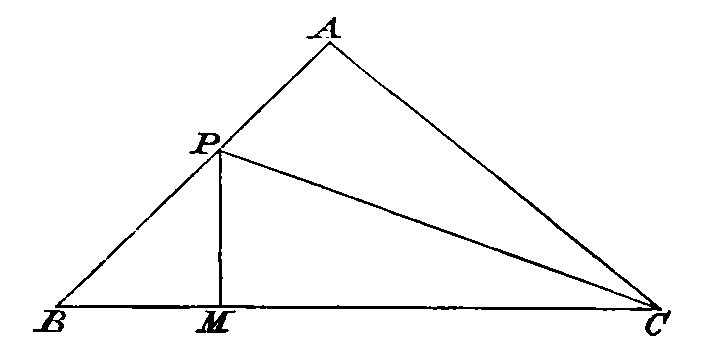
\includegraphics[width=0.6\textwidth]{508.png}
\centering
\end{figure}

Suppose \(P\) the origin of polar coordinates, in the plane of the
triangle; and take the initial line parallel to \(BC\).

The attraction of the infinite rod parallel to the edges of the
prism which corresponds to the polar element \(rdr\,d\theta\) is \(\xp\dfrac{2}{r}\,rdr\,d\theta\),
where the density is taken to be unity.

Consider first the prism corresponding to \(PBC\).

The attraction of a rod will be \(2 \cos\theta dr d\theta\) parallel to \(BC\),
and \(2\sin\theta dr d\theta\) perpendicular to \(BC\). Let the perpendicular
\(PM\) be denoted by \(h\). Then we must integrate for \(r\) from \(0\) to
\(\xp\dfrac{h}{\sin\theta}\); and we must integrate for \(\theta\) from \(\alpha\) to \(\beta\), where \(\alpha\) is equal
to \(PCB\), and \(\beta\) exceeds \(\alpha\) by \(BPC\). Thus the component attractions
are \(2h \log \xp\dfrac{\sin\beta}{\sin\alpha}\) parallel to \(BC\), and \(2h(\beta-\alpha)\) perpendicular
to \(BC\).

Similarly for the prism corresponding to \(PAC\) we find that
the component attractions are \(2h_1 \log \xp\dfrac{\sin\beta_1}{\sin\alpha_1}\) parallel to \(AC\), and
\(2h_1(\beta_1-\alpha_1)\) perpendicular to \(AC\); where \(h_1\) denotes the perpendicular
from \(P\) on \(AC\), and \(\alpha_1\) is equal to \(PCA\), and \(\beta_1-\alpha_1\) to \(APC\).
%%-----File: 509.png-----%%

Hence the attraction of the whole prism corresponding to \(ABC\)
parallel to \(BC\) is
\[2h \log \frac{\sin\beta}{\sin\alpha} + 2h_{1} \cos C \log \frac{\sin\beta_{1}}{\sin\alpha_{1}}+2h_{1} \sin C(\beta_{1}-\alpha_{1})\text{.}\]

This expression may be made to involve only one variable \(\alpha\); and
then we can seek the maximum value by putting the differential
coefficient with respect to \(\alpha\) zero. The equations which serve to
express the other variables in terms of \(\alpha\) are
\begin{align*}
&h (\cot B + \cot \alpha) = BC,\\
&h BC + h_{1} AC =\text{ twice the area of } ABC,\\
&\beta = \pi - B,\\
&\alpha_{1} + \alpha = C,\\
&\beta_{1} - \alpha_{1} = B + \alpha\text{.}
\end{align*}

Hutton instead of taking the whole prism supposes another
plane to pass through \(PM\), and to make an infinitesimal angle with
the plane of the paper. Thus he obtains a slice in the form of a
double wedge; he estimates the resolved attraction of the slice,
and assumes that this will represent the attraction of the whole
prism. He says:

\begin{squote}
And then from the foregoing suppositions it is evident that in
whatever point of \(AB\) the attraction of \(ABC\) is greatest, there also will
the attraction of the whole hill be the greatest.
\end{squote}

This assertion is unjustifiable. After I wrote this I found
that to this sentence Hutton adds the words ``very nearly,'' in the
abridgement of the memoir which is given in the \textit{Philosophical
Transactions abridged} by Hutton, Shaw and Pearson; and also
in the republication of the memoir in Hutton's \textit{Tracts}, Vol.\ \textsc{ii}.

Hutton considers especially the case in which the triangle
\(ABC\) is equilateral.

Suppose, for example, that \(P\) is at \(B\). Put \(c\) for \(AB\). Then
\(h=0\), \(h_{1} = \xp\dfrac{c\xsurd 3}{2}\), \(\alpha_{1} = \xp\dfrac{\pi}{3}\), \(\beta_{1}=\xp\dfrac{2\pi}{3}\). The attraction parallel to \(BC\)
\[=2\ldot\frac{c\xsurd3}{2}\ldot\frac{\xsurd3}{2}\ldot\frac{\pi}{3} = \frac{c\pi}{2}\text{.}\]
%%-----File: 510.png-----%%

Next suppose that \(P\) is at the middle point of \(AB\). Then
\[h_{1} = h = \frac{c \xsurd3}{4},\quad \alpha = \frac{\pi}{6},\quad \beta = \frac{2\pi}{3},\quad \alpha_{1} = \frac{\pi}{6},\quad \beta_{1}=\frac{2\pi}{3}\text{.}\]

The attraction parallel to \(BC\)
\[= \frac{c\xsurd 3}{2}\log\xsurd 3 + \frac{c\xsurd 3}{4}\log\xsurd 3 + \frac{c\xsurd 3}{2}.\frac{\xsurd 3}{2}.\frac{\pi}{2}=c\frac{3\xsurd 3}{4}\log\xsurd 3+\frac{3c\pi}{8}\text{.}\]

The ratio of the latter to the former
\[=\frac{3}{4} + \frac{3\xsurd 3}{2\pi}\log\xsurd 3 = \frac{3}{4}\left(1 + \frac{\xsurd 3}{\pi}\log 3\right)\text{.}\]

This is obviously the ratio of the whole attraction at \(B\) to the
whole attraction midway between \(A\) and \(B\); for each whole
attraction is inclined at \(30°\) to the horizon.

This will be found \(1·204\) approximately.

Hutton's theoretical expression for the ratio is quite different;
but numerically it is nearly the same: he gives almost \(1·206\).
The coincidence is curious.

\Section
737. Here we may be said to finish the first part of our
work; the history has been carried through a period of nearly
a century, from the publication of the \textit{Principia}, in which Newton
laid the solid foundations of the Theories of Attraction and of the
Figure of the Earth. Maclaurin and Clairaut continued the work
with great success; the former mainly devoting himself to the
Theory of Attraction, and the latter to that of the Figure of the
Earth. The incessant labours of D'Alembert effected more indirectly
than directly; they kept up an interest in the subjects,
and probably suggested the more fortunate efforts of Legendre
and Laplace. In the second volume we shall trace the progress
of our Theories under the influence of the powerful analysis of
these two great mathematicians.

\Section
738. Some publications are recorded in La Lande's \textit{Bibliographie
Astronomique} bearing on our subject, which I have not been
able to consult; although I believe they are of small importance,
I will quote the titles here, adding the pages of La Lande's
work where they are given.
%%-----File: 511.png-----%%

1735. \textit{Paris, in-12}. Proposition d'une mesure de la terre,
dont il résulte une diminution considérable dans la circonférence
de l'équateur, par M. D'Anville, géographe ordinaire du roi\dots.
Page 400.

1738. \dots\ \textit{in-12}. Anecdotes physiques et morales. Page 407.

A notice of this in La Lande's work follows immediately after
that of the \textit{Examen desintéressé}; he says it is on the same subject:
see Art.\ 143.

1740. \textit{Bologna, in-8\textsuperscript{o}}. Lettera contenente l'aviso delle operazioni
fatte nell' America meridionale dai matematici spagnuoli e
francesi, per cui venne a conchiudersi la gran controversia sopra
la figura della terra. Page 412.

1743. \textit{Viennæ, in-8\textsuperscript{o}}. De figurâ telluris dialogus à scholasticis
universitatis Viennensis. Page 422.

1744. \textit{Stockholm, in-8\textsuperscript{o}}. \dots\ Klingenstierna, \dots\ donna le problème
suivant: \textit{Trouver la figure de la terre par la comparaison
de deux degrés.} Page 424.

1748. \textit{London, in-8\textsuperscript{o}}. A new theory of the figure of the
earth, wherein are demonstrated the mechanical causes of its
figure as it is determined by the observations of Rowland Jackson.
Page 433.

1748. \textit{Tournay, in-8\textsuperscript{o}}. Discours sur ta figure de la terre,
par M. le baron de Grante. Page 435.

1763. \textit{Manhemii, in-4\textsuperscript{o}}. Basis Palatina, anno 1762 bis dimensa,
hoc anno 1763 novis mensuris aucta et confirmata, à
Christiano Mayer\dots. Page 483; see also page 503.

1766. \textit{Pisa, in-8\textsuperscript{o}}. Ragionamento filosofico-historico sopra la
figura della terra, dal S\textsuperscript{r}. Ant. Mattuni. Page 496.

1769. \textit{Vlissengen, in-8\textsuperscript{o}}. \dots\ On trouve dans le troisième
volume un mémoire de M. Hennert sur la figure de la terre, \dots\
Page 509.

1778. \textit{Utrecht, in-8\textsuperscript{o}}. Dissertations physiques et mathématiques,
sur la figure de la terre, les comètes, l'attraction, \&c., par
M. Hennert. Page 562.

1778. \textit{Varsaviæ, in-8\textsuperscript{o}}. Michaelis Hube, De telluris formâ.
Page 563.
%%-----File: 512.png-----%%

\Section
739. I hope that few of the memoirs which are contained in
the collections of the various Academies and Scientific Societies
have been overlooked. In seeking for these the well-known
\textit{Repertorium Commentationum} of J. D. Reuss affords most valuable
assistance. Here I find memoirs by four authors recorded which
I have not been able to consult, namely Celsius, Klingenstierna,
Mallet, and Fester: the titles occur in the fifth volume of the
work on the pages 80, 82, and 83.

\Section
740. There are three matters considered in the present
volume to which it will be convenient to allude here.

The difficulty which is mentioned in Art.\ 124 is discussed in
Art.\ 725.

Since Art.\ 228 was printed I have been informed by
M. O. Struve, that Delisle's original manuscripts were found some
years since at St Petersburg: those at Paris were copies.

Since Art.\ 542 was printed I have published some remarks on
the modern South African arc in the \textit{Monthly Notices of the Royal
Astronomical Society}, Vol.\ \textsc{xxxiii}.\ pages 27\dots 34.

\begin{center}
\vfill
\footnotesize
END OF VOLUME I.
\vfill
\vfill
\scriptsize
\longbar{CAMBRIDGE: PRINTED BY C. J. CLAY, M.A., AT THE UNIVERSITY PRESS.}
\end{center}
\clearpage

%%%% transcriber's note %%%%
\newpage
\thispagestyle{empty}
\begin{center}
Transcriber's notes
\vspace*{0.5cm}
\end{center}
\raggedright{
\small
An occasional missing accent on the word `Céleste' has been added.
Otherwise, inconsistent spelling has been retained.

In \hyperlink{257:1}{the equation} following `Since\ldots, we obtain' in section 257
it seems likely that the \(a\) in the denominator of the right hand side
should be primed but this change has not been made.

The prime on \(j\) in \hyperlink{289:1}{this equation} in section 289 seems dubious.

In \hyperlink{504:1}{the expression} on the line following `so that the definite
integral\ldots' in section 504
there appears to be a missing closing square bracket.

The following changes have been made:

`= 0' has been added to \hyperref[426:2]{equation 2} in section 426.

`the result becomes \(16\pi\rho h\)' in \hyperlink{472:1}{section 472} has been changed to
`the result becomes \(16\pi\rho r\)'.

`+' has been added before \(mM \cos^{m-1} \beta\) in \hyperref[576:1]{equation 2} in section 576.

The sentence \hyperlink{629:1}{`Similarly the other equations\ldots'} in section 629 is made
into a paragraph with a capital letter.}

\PGLicense
\begin{PGtext}
\begin{center}
*** END OF THE PROJECT GUTENBERG EBOOK A history of the mathematical theories of attraction and the figure of the earth from the time of Newton to that of Laplace. Volume 1 ***
\end{center}
\InputIfFileExists{pgfooter.tex}{}{}
\end{PGtext}
\end{document}
